\documentclass[a4paper]{book}
\usepackage{a4wide}
\usepackage{makeidx}
\usepackage{fancyhdr}
\usepackage{graphicx}
\usepackage{multicol}
\usepackage{float}
\usepackage{textcomp}
\usepackage{alltt}
\usepackage{times}
\ifx\pdfoutput\undefined
\usepackage[ps2pdf,
            pagebackref=true,
            colorlinks=true,
            linkcolor=blue
           ]{hyperref}
\usepackage{pspicture}
\else
\usepackage[pdftex,
            pagebackref=true,
            colorlinks=true,
            linkcolor=blue
           ]{hyperref}
\fi
\usepackage{doxygen}
\usepackage{amsmath}
\usepackage{amssymb}
\makeindex
\setcounter{tocdepth}{1}
\renewcommand{\footrulewidth}{0.4pt}
\begin{document}
\begin{titlepage}
\vspace*{7cm}
\begin{center}
{\Large NFFT Reference Manual\\[1ex]\large 3.0.3 }\\
\vspace*{1cm}
{\large Generated by Doxygen 1.4.1}\\
\vspace*{0.5cm}
{\small Mon Feb 5 23:37:37 2007}\\
\end{center}
\end{titlepage}
\clearemptydoublepage
\pagenumbering{roman}
\tableofcontents
\clearemptydoublepage
\pagenumbering{arabic}
\chapter{NFFT Main Page}
\label{index}\hypertarget{index}{}\hypertarget{index_section_intro_sec}{}\section{Introduction}\label{index_section_intro_sec}
Fast Fourier transforms (FFTs) belong to the '10 algorithms with the greatest influence on the development and practice of science and engineering in the 20th century'. The classic algorithm computes the discrete Fourier transform \[ f_j= \sum_{k=-\frac{N}{2}}^{\frac{N}{2}-1} \hat{f}_{k} {\rm e}^{2\pi{\rm i}\frac{kj}{N}} \] for $j=-\frac{N}{2},\hdots,\frac{N}{2}-1$ and given complex coefficients $\hat{f}_{k}\in\mathbb{C}$. Using a divide and conquer approach, the number of floating point operations is reduced from ${\cal O}(N^2)$ for a straightforward computation to only ${\cal O}(N\log N)$. In conjunction with publicly available efficient implementations the fast Fourier transform has become of great importance in scientific computing.

However, two shortcomings of traditional schemes are the need for equispaced sampling and the restriction to the system of complex exponential functions. The NFFT is a C subroutine library for computing the nonequispaced discrete Fourier transform (NDFT) and its generalisations in one or more dimensions, of arbitrary input size, and of complex data.

More precisely,we collect the possible frequencies $\mathbf{k}\in\mathbb{Z}^d$ in the multi-index set \[ I_{\mathbf{N}} := \left\{ \mathbf{k}=\left(k_t\right)_{t=0,\hdots,d-1} \in \mathbb{Z}^d: - \frac{N_t}{2} \le k_t < \frac{N_t}{2} ,\;t=0,\hdots,d-1\right\}, *\] where $\mathbf{N}=\left(N_t\right)_{t=0,\hdots,d-1}$ is the multibandlimit, i.e., $N_t\in 2\mathbb{N}$. For a finite number of given Fourier coefficients $\hat f_{\mathbf{k}} \in \mathbb{C}$, $\mathbf{k}\in I_{\mathbf{N}}$, we consider the fast evaluation of the trigonometric polynomial \[ f\left(\mathbf{x}\right) := \sum_{ \mathbf{k}\in I_{ N}} \hat{f}_{\mathbf{ k}} {\rm e}^{-2\pi{\rm i}\mathbf{k}\mathbf{ x}} \] at given nonequispaced nodes $\mathbf{x}_j \in \mathbb{T}^d$, $j=0,\ldots, M-1$, from the $ d$-dimensional torus as well as the adjoint problem, the fast evaluation of sums of the form \[ \hat h_{\mathbf{k}} := \sum_{j=0}^{M-1} {f}_{j} {\rm e}^{2\pi{\rm i}\mathbf{k}\mathbf{ x}_j}. \]

The generalisations of the NFFT include\begin{itemize}
\item NNFFT - nonequispaced in time and frequency fast Fourier transform,\item NFCT/NFST - nonequispaced fast (co)sine transform,\item NSFFT - nonequispaced sparse fast Fourier transform,\item FPT - fast polynomial transform,\item NFSFT - nonequispaced fast spherical Fourier transform.\end{itemize}


Furthermore, we consider the inversion of the above transforms by iterative methods. 
\chapter{NFFT Module Index}
\section{NFFT Modules}
Here is a list of all modules:\begin{CompactList}
\item \contentsline{section}{NFFT - Nonequispaced fast Fourier transform}{\pageref{group__nfft}}{}
\item \contentsline{section}{NFCT/NFST - Nonequispaced fast (co)sine transform}{\pageref{group__nfsct}}{}
\item \contentsline{section}{NNFFT - Nonequispaced in time and frequency FFT}{\pageref{group__nnfft}}{}
\item \contentsline{section}{NSFFT - Nonequispaced sparse FFT}{\pageref{group__nsfft}}{}
\item \contentsline{section}{MRI - Transforms in magnetic resonance imaging}{\pageref{group__mri}}{}
\item \contentsline{section}{NFSFT - Nonequispaced fast spherical Fourier transform}{\pageref{group__nfsft}}{}
\item \contentsline{section}{FPT - Fast polynomial transform}{\pageref{group__fpt}}{}
\item \contentsline{section}{Solver - Inverse transforms}{\pageref{group__solver}}{}
\item \contentsline{section}{Util - Auxilliary functions}{\pageref{group__nfftutil}}{}
\item \contentsline{section}{Examples}{\pageref{group__examples}}{}
\begin{CompactList}
\item \contentsline{section}{Solver component}{\pageref{group__examples__solver}}{}
\begin{CompactList}
\item \contentsline{section}{Reconstruction of a glacier from scattered data}{\pageref{group__examples__solver__glacier}}{}
\item \contentsline{section}{Simple inverse nfft}{\pageref{group__examples__solver__simple}}{}
\end{CompactList}
\end{CompactList}
\item \contentsline{section}{Applications}{\pageref{group__applications}}{}
\begin{CompactList}
\item \contentsline{section}{Fast Gauss transfrom with complex parameter}{\pageref{group__applications__fastgauss}}{}
\item \contentsline{section}{Fast summation}{\pageref{group__applications__fastsum}}{}
\begin{CompactList}
\item \contentsline{section}{fastsum\_\-matlab}{\pageref{group__applications__fastsum__matlab}}{}
\item \contentsline{section}{fastsum\_\-test}{\pageref{group__applications__fastsum__test}}{}
\end{CompactList}
\item \contentsline{section}{Fast summation of radial functions on the sphere}{\pageref{group__applications__fastsumS2}}{}
\begin{CompactList}
\item \contentsline{section}{fastsum\-S2\_\-matlab}{\pageref{group__applications__fastsumS2__test}}{}
\end{CompactList}
\item \contentsline{section}{Iterative reconstruction on the sphere S2}{\pageref{group__applications__iterS2}}{}
\begin{CompactList}
\item \contentsline{section}{iter\-S2\_\-matlab}{\pageref{group__applications__iterS2__matlab}}{}
\end{CompactList}
\item \contentsline{section}{Transforms in magnetic resonance imaging}{\pageref{group__applications__mri}}{}
\begin{CompactList}
\item \contentsline{section}{2D transforms}{\pageref{group__applications__mri2d}}{}
\begin{CompactList}
\item \contentsline{section}{construct\_\-data\_\-2d}{\pageref{group__applications__mri2d__construct__data__2d}}{}
\item \contentsline{section}{construct\_\-data\_\-\_\-inh\_\-2d1d}{\pageref{group__applications__mri2d__construct__data__inh__2d1d}}{}
\item \contentsline{section}{construct\_\-data\_\-inh\_\-3d}{\pageref{group__applications__mri2d__construct__data__inh__3d}}{}
\item \contentsline{section}{reconstruct\_\-data\_\-2d}{\pageref{group__applications__mri2d__reconstruct__data__2d}}{}
\item \contentsline{section}{construct\_\-data\_\-gridding}{\pageref{group__applications__mri2d__construct__data__gridding}}{}
\item \contentsline{section}{reconstruct\_\-data\_\-\_\-inh\_\-2d1d}{\pageref{group__applications__mri2d__reconstruct__data__inh__2d1d}}{}
\item \contentsline{section}{reconstruct\_\-data\_\-inh\_\-3d}{\pageref{group__applications__mri2d__reconstruct__data__inh__3d}}{}
\item \contentsline{section}{construct\_\-data\_\-inh\_\-nnfft}{\pageref{group__applications__mri2d__construct__data__inh__nnfft}}{}
\end{CompactList}
\item \contentsline{section}{3D transforms}{\pageref{group__applications__mri3d}}{}
\begin{CompactList}
\item \contentsline{section}{construct\_\-data\_\-1d2d}{\pageref{group__applications__mri3d__construct__data__1d2d}}{}
\item \contentsline{section}{construct\_\-data\_\-3d}{\pageref{group__applications__mri3d__construct__data__3d}}{}
\item \contentsline{section}{reconstruct\_\-data\_\-1d2d}{\pageref{group__applications__mri3d__reconstruct__data__1d2d}}{}
\item \contentsline{section}{reconstruct\_\-data\_\-3d}{\pageref{group__applications__mri3d__reconstruct__data__3d}}{}
\item \contentsline{section}{reconstruct\_\-data\_\-gridding}{\pageref{group__applications__mri3d__reconstruct__data__gridding}}{}
\end{CompactList}
\end{CompactList}
\item \contentsline{section}{Polar FFT}{\pageref{group__applications__polarFFT}}{}
\begin{CompactList}
\item \contentsline{section}{linogram\_\-fft\_\-test}{\pageref{group__applications__polarFFT__linogramm}}{}
\item \contentsline{section}{mpolar\_\-fft\_\-test}{\pageref{group__applications__polarFFT__mpolar}}{}
\item \contentsline{section}{polar\_\-fft\_\-test}{\pageref{group__applications__polarFFT__polar}}{}
\end{CompactList}
\item \contentsline{section}{Fast evaluation of quadrature formulae on the sphere}{\pageref{group__applications__quadratureS2}}{}
\begin{CompactList}
\item \contentsline{section}{quadrature\-S2\_\-test}{\pageref{group__applications__quadratureS2__test}}{}
\end{CompactList}
\end{CompactList}
\end{CompactList}

\chapter{NFFT Directory Hierarchy}
\section{NFFT Directories}
This directory hierarchy is sorted roughly, but not completely, alphabetically:\begin{CompactList}
\item \contentsline{section}{applications}{\pageref{dir_000006}}{}
\begin{CompactList}
\item \contentsline{section}{fastgauss}{\pageref{dir_000015}}{}
\item \contentsline{section}{fastsum}{\pageref{dir_000016}}{}
\item \contentsline{section}{fastsum\-S2}{\pageref{dir_000011}}{}
\item \contentsline{section}{iter\-S2}{\pageref{dir_000012}}{}
\item \contentsline{section}{mri}{\pageref{dir_000007}}{}
\begin{CompactList}
\item \contentsline{section}{mri2d}{\pageref{dir_000008}}{}
\item \contentsline{section}{mri3d}{\pageref{dir_000009}}{}
\end{CompactList}
\item \contentsline{section}{polar\-FFT}{\pageref{dir_000013}}{}
\item \contentsline{section}{potential}{\pageref{dir_000017}}{}
\item \contentsline{section}{quadrature\-S2}{\pageref{dir_000014}}{}
\item \contentsline{section}{radon}{\pageref{dir_000022}}{}
\end{CompactList}
\item \contentsline{section}{examples}{\pageref{dir_000000}}{}
\begin{CompactList}
\item \contentsline{section}{fpt}{\pageref{dir_000030}}{}
\item \contentsline{section}{nfct}{\pageref{dir_000020}}{}
\begin{CompactList}
\item \contentsline{section}{func\_\-rec\_\-2d}{\pageref{dir_000021}}{}
\end{CompactList}
\item \contentsline{section}{nfft}{\pageref{dir_000018}}{}
\item \contentsline{section}{nfsft}{\pageref{dir_000031}}{}
\item \contentsline{section}{nfst}{\pageref{dir_000032}}{}
\item \contentsline{section}{nnfft}{\pageref{dir_000001}}{}
\begin{CompactList}
\item \contentsline{section}{accuracy}{\pageref{dir_000002}}{}
\item \contentsline{section}{simple\_\-test}{\pageref{dir_000033}}{}
\end{CompactList}
\item \contentsline{section}{nsfft}{\pageref{dir_000029}}{}
\item \contentsline{section}{solver}{\pageref{dir_000010}}{}
\end{CompactList}
\item \contentsline{section}{include}{\pageref{dir_000005}}{}
\item \contentsline{section}{kernel}{\pageref{dir_000003}}{}
\begin{CompactList}
\item \contentsline{section}{fpt}{\pageref{dir_000019}}{}
\item \contentsline{section}{mri}{\pageref{dir_000023}}{}
\item \contentsline{section}{nfct}{\pageref{dir_000024}}{}
\item \contentsline{section}{nfft}{\pageref{dir_000025}}{}
\item \contentsline{section}{nfsft}{\pageref{dir_000004}}{}
\item \contentsline{section}{nfst}{\pageref{dir_000026}}{}
\item \contentsline{section}{nnfft}{\pageref{dir_000027}}{}
\item \contentsline{section}{nsfft}{\pageref{dir_000028}}{}
\item \contentsline{section}{solver}{\pageref{dir_000034}}{}
\end{CompactList}
\item \contentsline{section}{util}{\pageref{dir_000035}}{}
\end{CompactList}

\chapter{NFFT Data Structure Index}
\section{NFFT Data Structures}
Here are the data structures with brief descriptions:\begin{CompactList}
\item\contentsline{section}{\hyperlink{structfastsum__plan__}{fastsum\_\-plan\_\-} (Plan for fast summation algorithm )}{\pageref{structfastsum__plan__}}{}
\item\contentsline{section}{\hyperlink{structfgt__plan}{fgt\_\-plan} (Structure for the Gauss transform )}{\pageref{structfgt__plan}}{}
\item\contentsline{section}{\hyperlink{structfields__fastsum__plan__}{fields\_\-fastsum\_\-plan\_\-} (Plan for fast calculation of 3D space-charge fields of bunches of charged particles )}{\pageref{structfields__fastsum__plan__}}{}
\item\contentsline{section}{\hyperlink{structfpt__data__}{fpt\_\-data\_\-} (Holds data for a single cascade summation )}{\pageref{structfpt__data__}}{}
\item\contentsline{section}{\hyperlink{structfpt__set__s__}{fpt\_\-set\_\-s\_\-} (Holds data for a set of cascade summations )}{\pageref{structfpt__set__s__}}{}
\item\contentsline{section}{\hyperlink{structfpt__step__}{fpt\_\-step\_\-} (Holds data for a single multiplication step in the cascade summation )}{\pageref{structfpt__step__}}{}
\item\contentsline{section}{\hyperlink{structimri__inh__2d1d__plan}{imri\_\-inh\_\-2d1d\_\-plan} (Structure for an inverse transform plan )}{\pageref{structimri__inh__2d1d__plan}}{}
\item\contentsline{section}{\hyperlink{structimri__inh__3d__plan}{imri\_\-inh\_\-3d\_\-plan} (Structure for an inverse transform plan )}{\pageref{structimri__inh__3d__plan}}{}
\item\contentsline{section}{\hyperlink{structinfct__plan}{infct\_\-plan} (Structure for an inverse transform plan )}{\pageref{structinfct__plan}}{}
\item\contentsline{section}{\hyperlink{structinfft__plan}{infft\_\-plan} (Structure for an inverse transform plan )}{\pageref{structinfft__plan}}{}
\item\contentsline{section}{\hyperlink{structinfsft__plan}{infsft\_\-plan} (Structure for an inverse transform plan )}{\pageref{structinfsft__plan}}{}
\item\contentsline{section}{\hyperlink{structinfst__plan}{infst\_\-plan} (Structure for an inverse transform plan )}{\pageref{structinfst__plan}}{}
\item\contentsline{section}{\hyperlink{structinnfft__plan}{innfft\_\-plan} (Structure for an inverse transform plan )}{\pageref{structinnfft__plan}}{}
\item\contentsline{section}{\hyperlink{structmri__inh__2d1d__plan}{mri\_\-inh\_\-2d1d\_\-plan} (The structure for the transform plan )}{\pageref{structmri__inh__2d1d__plan}}{}
\item\contentsline{section}{\hyperlink{structmri__inh__3d__plan}{mri\_\-inh\_\-3d\_\-plan} (The structure for the transform plan )}{\pageref{structmri__inh__3d__plan}}{}
\item\contentsline{section}{\hyperlink{structnfct__plan}{nfct\_\-plan} (Structure for a transform plan )}{\pageref{structnfct__plan}}{}
\item\contentsline{section}{\hyperlink{structnfft__plan}{nfft\_\-plan} (Structure for a NFFT plan )}{\pageref{structnfft__plan}}{}
\item\contentsline{section}{\hyperlink{structnfsft__plan}{nfsft\_\-plan} (Structure for a NFSFT transform plan )}{\pageref{structnfsft__plan}}{}
\item\contentsline{section}{\hyperlink{structnfsft__wisdom}{nfsft\_\-wisdom} (Wisdom structure )}{\pageref{structnfsft__wisdom}}{}
\item\contentsline{section}{\hyperlink{structnfst__plan}{nfst\_\-plan} (Structure for a transform plan )}{\pageref{structnfst__plan}}{}
\item\contentsline{section}{\hyperlink{structnnfft__plan}{nnfft\_\-plan} (Structure for a transform plan )}{\pageref{structnnfft__plan}}{}
\item\contentsline{section}{\hyperlink{structnsfft__plan}{nsfft\_\-plan} (Structure for a NFFT plan )}{\pageref{structnsfft__plan}}{}
\item\contentsline{section}{\hyperlink{structwindow__funct__plan__}{window\_\-funct\_\-plan\_\-} (Window\_\-funct\_\-plan is a plan to use the window functions independent of the nfft )}{\pageref{structwindow__funct__plan__}}{}
\end{CompactList}

\chapter{NFFT File Index}
\section{NFFT File List}
Here is a list of all documented files with brief descriptions:\begin{CompactList}
\item\contentsline{section}{\textbf{accuracy.c} }{\pageref{accuracy_8c}}{}
\item\contentsline{section}{\hyperlink{api_8h}{api.h} }{\pageref{api_8h}}{}
\item\contentsline{section}{\textbf{config.h} }{\pageref{config_8h}}{}
\item\contentsline{section}{\textbf{construct\_\-data\_\-2d.c} }{\pageref{construct__data__2d_8c}}{}
\item\contentsline{section}{\textbf{construct\_\-data\_\-2d1d.c} }{\pageref{construct__data__2d1d_8c}}{}
\item\contentsline{section}{\textbf{construct\_\-data\_\-3d.c} }{\pageref{construct__data__3d_8c}}{}
\item\contentsline{section}{\textbf{construct\_\-data\_\-inh\_\-2d1d.c} }{\pageref{construct__data__inh__2d1d_8c}}{}
\item\contentsline{section}{\textbf{construct\_\-data\_\-inh\_\-3d.c} }{\pageref{construct__data__inh__3d_8c}}{}
\item\contentsline{section}{\textbf{doxygen.c} }{\pageref{doxygen_8c}}{}
\item\contentsline{section}{\textbf{examples/doxygen.c} }{\pageref{examples_2doxygen_8c}}{}
\item\contentsline{section}{\textbf{examples/solver/doxygen.c} }{\pageref{examples_2solver_2doxygen_8c}}{}
\item\contentsline{section}{\textbf{applications/doxygen.c} }{\pageref{applications_2doxygen_8c}}{}
\item\contentsline{section}{\textbf{applications/fastsumS2/doxygen.c} }{\pageref{applications_2fastsumS2_2doxygen_8c}}{}
\item\contentsline{section}{\textbf{applications/iterS2/doxygen.c} }{\pageref{applications_2iterS2_2doxygen_8c}}{}
\item\contentsline{section}{\textbf{applications/mri/doxygen.c} }{\pageref{applications_2mri_2doxygen_8c}}{}
\item\contentsline{section}{\textbf{applications/mri/mri2d/doxygen.c} }{\pageref{applications_2mri_2mri2d_2doxygen_8c}}{}
\item\contentsline{section}{\textbf{applications/mri/mri3d/doxygen.c} }{\pageref{applications_2mri_2mri3d_2doxygen_8c}}{}
\item\contentsline{section}{\textbf{applications/polarFFT/doxygen.c} }{\pageref{applications_2polarFFT_2doxygen_8c}}{}
\item\contentsline{section}{\textbf{applications/quadratureS2/doxygen.c} }{\pageref{applications_2quadratureS2_2doxygen_8c}}{}
\item\contentsline{section}{\textbf{fastgauss.c} }{\pageref{fastgauss_8c}}{}
\item\contentsline{section}{\hyperlink{fastsum_8c}{fastsum.c} (Fast NFFT-based summation algorithm )}{\pageref{fastsum_8c}}{}
\item\contentsline{section}{\hyperlink{fastsum_8h}{fastsum.h} (Header file for the fast NFFT-based summation algorithm )}{\pageref{fastsum_8h}}{}
\item\contentsline{section}{\hyperlink{fastsum__matlab_8c}{fastsum\_\-matlab.c} (Simple test program for the fast NFFT-based summation algorithm, called by fastsum.m )}{\pageref{fastsum__matlab_8c}}{}
\item\contentsline{section}{\hyperlink{fastsum__test_8c}{fastsum\_\-test.c} (Simple test program for the fast NFFT-based summation algorithm )}{\pageref{fastsum__test_8c}}{}
\item\contentsline{section}{\textbf{fastsumS2.c} }{\pageref{fastsumS2_8c}}{}
\item\contentsline{section}{\hyperlink{fields__fastsum_8c}{fields\_\-fastsum.c} (Calculation of 3d space-charge fields of bunches of charged particles by fast summation )}{\pageref{fields__fastsum_8c}}{}
\item\contentsline{section}{\hyperlink{fields__fastsum_8h}{fields\_\-fastsum.h} (Header file for calculation of 3d space-charge fields of bunches of charged particles by fast summation )}{\pageref{fields__fastsum_8h}}{}
\item\contentsline{section}{\textbf{fields\_\-fastsum\_\-matlab.c} }{\pageref{fields__fastsum__matlab_8c}}{}
\item\contentsline{section}{\hyperlink{fields__fastsum__test_8c}{fields\_\-fastsum\_\-test.c} (Simple test program for the fast NFFT-based calculation of 3D space-charge fields of bunches of charged particles )}{\pageref{fields__fastsum__test_8c}}{}
\item\contentsline{section}{\hyperlink{flags_8c}{flags.c} (Testing the nfft )}{\pageref{flags_8c}}{}
\item\contentsline{section}{\hyperlink{fpt_8c}{fpt.c} }{\pageref{fpt_8c}}{}
\item\contentsline{section}{\textbf{fpt.h} }{\pageref{fpt_8h}}{}
\item\contentsline{section}{\textbf{func\_\-rec\_\-2d.c} }{\pageref{func__rec__2d_8c}}{}
\item\contentsline{section}{\textbf{glacier.c} }{\pageref{glacier_8c}}{}
\item\contentsline{section}{\textbf{infft.h} }{\pageref{infft_8h}}{}
\item\contentsline{section}{\hyperlink{inverse__radon_8c}{inverse\_\-radon.c} }{\pageref{inverse__radon_8c}}{}
\item\contentsline{section}{\textbf{iterS2.c} }{\pageref{iterS2_8c}}{}
\item\contentsline{section}{\hyperlink{kernels_8c}{kernels.c} (File with predefined kernels for the fast summation algorithm )}{\pageref{kernels_8c}}{}
\item\contentsline{section}{\hyperlink{kernels_8h}{kernels.h} (Header file with predefined kernels for the fast summation algorithm )}{\pageref{kernels_8h}}{}
\item\contentsline{section}{\textbf{legendre.c} }{\pageref{legendre_8c}}{}
\item\contentsline{section}{\textbf{legendre.h} }{\pageref{legendre_8h}}{}
\item\contentsline{section}{\hyperlink{linogram__fft__test_8c}{linogram\_\-fft\_\-test.c} }{\pageref{linogram__fft__test_8c}}{}
\item\contentsline{section}{\textbf{malloc.c} }{\pageref{malloc_8c}}{}
\item\contentsline{section}{\hyperlink{mpolar__fft__test_8c}{mpolar\_\-fft\_\-test.c} }{\pageref{mpolar__fft__test_8c}}{}
\item\contentsline{section}{\textbf{mri.c} }{\pageref{mri_8c}}{}
\item\contentsline{section}{\hyperlink{ndft__fast_8c}{ndft\_\-fast.c} (Testing ndft, Horner-like ndft, and fully precomputed ndft )}{\pageref{ndft__fast_8c}}{}
\item\contentsline{section}{\textbf{nfct.c} }{\pageref{nfct_8c}}{}
\item\contentsline{section}{\textbf{nfft.c} }{\pageref{nfft_8c}}{}
\item\contentsline{section}{\hyperlink{nfft3_8h}{nfft3.h} (Header file for the nfft3 library )}{\pageref{nfft3_8h}}{}
\item\contentsline{section}{\textbf{nfft\_\-times.c} }{\pageref{nfft__times_8c}}{}
\item\contentsline{section}{\textbf{nfftconf.h} }{\pageref{nfftconf_8h}}{}
\item\contentsline{section}{\hyperlink{nfsft_8c}{nfsft.c} }{\pageref{nfsft_8c}}{}
\item\contentsline{section}{\textbf{nfsoft.c} }{\pageref{nfsoft_8c}}{}
\item\contentsline{section}{\textbf{nfst.c} }{\pageref{nfst_8c}}{}
\item\contentsline{section}{\textbf{nnfft.c} }{\pageref{nnfft_8c}}{}
\item\contentsline{section}{\textbf{nsfft.c} }{\pageref{nsfft_8c}}{}
\item\contentsline{section}{\textbf{nsfft\_\-test.c} }{\pageref{nsfft__test_8c}}{}
\item\contentsline{section}{\hyperlink{polar__fft__test_8c}{polar\_\-fft\_\-test.c} }{\pageref{polar__fft__test_8c}}{}
\item\contentsline{section}{\textbf{quadratureS2.c} }{\pageref{quadratureS2_8c}}{}
\item\contentsline{section}{\hyperlink{radon_8c}{radon.c} }{\pageref{radon_8c}}{}
\item\contentsline{section}{\textbf{reconstruct\_\-data\_\-2d.c} }{\pageref{reconstruct__data__2d_8c}}{}
\item\contentsline{section}{\textbf{reconstruct\_\-data\_\-2d1d.c} }{\pageref{reconstruct__data__2d1d_8c}}{}
\item\contentsline{section}{\textbf{reconstruct\_\-data\_\-3d.c} }{\pageref{reconstruct__data__3d_8c}}{}
\item\contentsline{section}{\textbf{mri2d/reconstruct\_\-data\_\-gridding.c} }{\pageref{mri2d_2reconstruct__data__gridding_8c}}{}
\item\contentsline{section}{\textbf{mri3d/reconstruct\_\-data\_\-gridding.c} }{\pageref{mri3d_2reconstruct__data__gridding_8c}}{}
\item\contentsline{section}{\textbf{reconstruct\_\-data\_\-inh\_\-2d1d.c} }{\pageref{reconstruct__data__inh__2d1d_8c}}{}
\item\contentsline{section}{\textbf{reconstruct\_\-data\_\-inh\_\-3d.c} }{\pageref{reconstruct__data__inh__3d_8c}}{}
\item\contentsline{section}{\textbf{reconstruct\_\-data\_\-inh\_\-nnfft.c} }{\pageref{reconstruct__data__inh__nnfft_8c}}{}
\item\contentsline{section}{\textbf{fpt/simple\_\-test.c} }{\pageref{fpt_2simple__test_8c}}{}
\item\contentsline{section}{\textbf{nfct/simple\_\-test.c} }{\pageref{nfct_2simple__test_8c}}{}
\item\contentsline{section}{\textbf{nfft/simple\_\-test.c} }{\pageref{nfft_2simple__test_8c}}{}
\item\contentsline{section}{\textbf{nfsft/simple\_\-test.c} }{\pageref{nfsft_2simple__test_8c}}{}
\item\contentsline{section}{\textbf{nfsoft/simple\_\-test.c} }{\pageref{nfsoft_2simple__test_8c}}{}
\item\contentsline{section}{\textbf{nfst/simple\_\-test.c} }{\pageref{nfst_2simple__test_8c}}{}
\item\contentsline{section}{\textbf{nnfft/simple\_\-test.c} }{\pageref{nnfft_2simple__test_8c}}{}
\item\contentsline{section}{\textbf{nsfft/simple\_\-test.c} }{\pageref{nsfft_2simple__test_8c}}{}
\item\contentsline{section}{\textbf{solver/simple\_\-test.c} }{\pageref{solver_2simple__test_8c}}{}
\item\contentsline{section}{\hyperlink{solver_8c}{solver.c} (Implementation file for the solver module )}{\pageref{solver_8c}}{}
\item\contentsline{section}{\hyperlink{solver__adjoint_8h}{solver\_\-adjoint.h} (Header file for adjoint solver )}{\pageref{solver__adjoint_8h}}{}
\item\contentsline{section}{\hyperlink{taylor__nfft_8c}{taylor\_\-nfft.c} (Testing the nfft againt a Taylor expansion based version )}{\pageref{taylor__nfft_8c}}{}
\item\contentsline{section}{\textbf{util.c} }{\pageref{util_8c}}{}
\item\contentsline{section}{\hyperlink{util_8h}{util.h} (Header file for utility functions used by the nfft3 library )}{\pageref{util_8h}}{}
\item\contentsline{section}{\textbf{wigner.c} }{\pageref{wigner_8c}}{}
\item\contentsline{section}{\hyperlink{wigner_8h}{wigner.h} }{\pageref{wigner_8h}}{}
\end{CompactList}

\chapter{NFFT Module Documentation}
\hypertarget{group__nfft}{
\section{NFFT - Nonequispaced fast Fourier transform}
\label{group__nfft}\index{NFFT - Nonequispaced fast Fourier transform@{NFFT - Nonequispaced fast Fourier transform}}
}
Direct and fast computation of the nonequispaced discrete Fourier transform.  
\subsection*{Data Structures}
\begin{CompactItemize}
\item 
struct \hyperlink{structnfft__plan}{nfft\_\-plan}
\begin{CompactList}\small\item\em Structure for a NFFT plan. \item\end{CompactList}\end{CompactItemize}
\subsection*{Defines}
\begin{CompactItemize}
\item 
\#define \hyperlink{group__nfft_gda3a356fdaf5840f98374a0a7aaf3e9c}{PRE\_\-PHI\_\-HUT}~(1U$<$$<$ 0)
\begin{CompactList}\small\item\em If this flag is set, the deconvolution step (the multiplication with the diagonal matrix $\mathbf{D}$) uses precomputed values of the Fourier transformed window function. \item\end{CompactList}\item 
\#define \hyperlink{group__nfft_g01ebac2d2071639df189f083fc9f24eb}{FG\_\-PSI}~(1U$<$$<$ 1)
\begin{CompactList}\small\item\em If this flag is set, the convolution step (the multiplication with the sparse matrix $\mathbf{B}$) uses particular properties of the Gaussian window function to trade multiplications for direct calls to exponential function. \item\end{CompactList}\item 
\#define \hyperlink{group__nfft_gbb1ad048b695cb806baf010c5d1b2caf}{PRE\_\-LIN\_\-PSI}~(1U$<$$<$ 2)
\begin{CompactList}\small\item\em If this flag is set, the convolution step (the multiplication with the sparse matrix $\mathbf{B}$) uses linear interpolation from a lookup table of equispaced samples of the window function instead of exact values of the window function. \item\end{CompactList}\item 
\#define \hyperlink{group__nfft_g9c5a5ab61009a801082897ca40a1658c}{PRE\_\-FG\_\-PSI}~(1U$<$$<$ 3)
\begin{CompactList}\small\item\em If this flag is set, the convolution step (the multiplication with the sparse matrix $\mathbf{B}$) uses particular properties of the Gaussian window function to trade multiplications for direct calls to exponential function (the remaining $2dM$ direct calls are precomputed). \item\end{CompactList}\item 
\#define \hyperlink{group__nfft_g959463a5c7723ccef5057ddcb784b40c}{PRE\_\-PSI}~(1U$<$$<$ 4)
\begin{CompactList}\small\item\em If this flag is set, the convolution step (the multiplication with the sparse matrix $\mathbf{B}$) uses $(2m+2)dM$ precomputed values of the window function. \item\end{CompactList}\item 
\#define \hyperlink{group__nfft_g7ad8a7e19519b16340dabec48899c6a4}{PRE\_\-FULL\_\-PSI}~(1U$<$$<$ 5)
\begin{CompactList}\small\item\em If this flag is set, the convolution step (the multiplication with the sparse matrix $\mathbf{B}$) uses $(2m+2)^dM$ precomputed values of the window function, in addition indices of source and target vectors are stored. \item\end{CompactList}\item 
\#define \hyperlink{group__nfft_g353185384f87de0dc4320a82652ef724}{MALLOC\_\-X}~(1U$<$$<$ 6)
\begin{CompactList}\small\item\em If this flag is set, (de)allocation of the node vector is done. \item\end{CompactList}\item 
\#define \hyperlink{group__nfft_g02d52cb02b6cfdbc3e4d5fd4de1aef9e}{MALLOC\_\-F\_\-HAT}~(1U$<$$<$ 7)
\begin{CompactList}\small\item\em If this flag is set, (de)allocation of the vector of Fourier coefficients is done. \item\end{CompactList}\item 
\#define \hyperlink{group__nfft_ga7b5098f4136080bbe0dd989973e2a69}{MALLOC\_\-F}~(1U$<$$<$ 8)
\begin{CompactList}\small\item\em If this flag is set, (de)allocation of the vector of samples is done. \item\end{CompactList}\item 
\#define \hyperlink{group__nfft_g9193f768d5839892d0e303080c370eaf}{FFT\_\-OUT\_\-OF\_\-PLACE}~(1U$<$$<$ 9)
\begin{CompactList}\small\item\em If this flag is set, FFTW uses disjoint input/output vectors. \item\end{CompactList}\item 
\#define \hyperlink{group__nfft_gd3fe6867a3351441c6f44dd5a3746f5b}{FFTW\_\-INIT}~(1U$<$$<$ 10)
\begin{CompactList}\small\item\em If this flag is set, fftw\_\-init/fftw\_\-finalize is called. \item\end{CompactList}\item 
\#define \hyperlink{group__nfft_g44c85197c6bdcf4b632aeff5e94d5329}{PRE\_\-ONE\_\-PSI}~(PRE\_\-LIN\_\-PSI$|$ PRE\_\-FG\_\-PSI$|$ PRE\_\-PSI$|$ PRE\_\-FULL\_\-PSI)
\begin{CompactList}\small\item\em Summarises if precomputation is used within the convolution step (the multiplication with the sparse matrix $\mathbf{B}$). \item\end{CompactList}\end{CompactItemize}
\subsection*{Functions}
\begin{CompactItemize}
\item 
void \hyperlink{group__nfft_g27ef1bcb8dd3a3fc1cdbeee368ec1acf}{ndft\_\-trafo} (\hyperlink{structnfft__plan}{nfft\_\-plan} $\ast$ths)
\begin{CompactList}\small\item\em Computes a NDFT, see the \hyperlink{group__nfft_ndft_formula}{definition}. \item\end{CompactList}\item 
void \hyperlink{group__nfft_g03975608fdf8cfd8757f1f52b43ec51b}{ndft\_\-adjoint} (\hyperlink{structnfft__plan}{nfft\_\-plan} $\ast$ths)
\begin{CompactList}\small\item\em Computes an adjoint NDFT, see the definition. \item\end{CompactList}\item 
void \hyperlink{group__nfft_g9f1e6bd9f7f956a8679e6b413c97b421}{nfft\_\-trafo} (\hyperlink{structnfft__plan}{nfft\_\-plan} $\ast$ths)
\begin{CompactList}\small\item\em Computes a NFFT, see the \hyperlink{group__nfft_ndft_formula}{definition}. \item\end{CompactList}\item 
\hypertarget{group__nfft_ge6dff0553d273fc53a15ce4535df8087}{
void \hyperlink{group__nfft_ge6dff0553d273fc53a15ce4535df8087}{nfft\_\-trafo\_\-1d} (\hyperlink{structnfft__plan}{nfft\_\-plan} $\ast$ths)}
\label{group__nfft_ge6dff0553d273fc53a15ce4535df8087}

\item 
\hypertarget{group__nfft_gc05ae265993ff8e1396ac6c801c47ffe}{
void \hyperlink{group__nfft_gc05ae265993ff8e1396ac6c801c47ffe}{nfft\_\-trafo\_\-2d} (\hyperlink{structnfft__plan}{nfft\_\-plan} $\ast$ths)}
\label{group__nfft_gc05ae265993ff8e1396ac6c801c47ffe}

\item 
\hypertarget{group__nfft_g503e48334b8cdefb63f55941460354bf}{
void \hyperlink{group__nfft_g503e48334b8cdefb63f55941460354bf}{nfft\_\-trafo\_\-3d} (\hyperlink{structnfft__plan}{nfft\_\-plan} $\ast$ths)}
\label{group__nfft_g503e48334b8cdefb63f55941460354bf}

\item 
void \hyperlink{group__nfft_g4b44c1dd52026dcb494dc735f0fa5b08}{nfft\_\-adjoint} (\hyperlink{structnfft__plan}{nfft\_\-plan} $\ast$ths)
\begin{CompactList}\small\item\em Computes an adjoint NFFT, see the definition. \item\end{CompactList}\item 
\hypertarget{group__nfft_g13f8052bab72ec8994354cdd6ccb6982}{
void \hyperlink{group__nfft_g13f8052bab72ec8994354cdd6ccb6982}{nfft\_\-adjoint\_\-1d} (\hyperlink{structnfft__plan}{nfft\_\-plan} $\ast$ths)}
\label{group__nfft_g13f8052bab72ec8994354cdd6ccb6982}

\item 
\hypertarget{group__nfft_gda6d6c809694e08aac88fa0204192325}{
void \hyperlink{group__nfft_gda6d6c809694e08aac88fa0204192325}{nfft\_\-adjoint\_\-2d} (\hyperlink{structnfft__plan}{nfft\_\-plan} $\ast$ths)}
\label{group__nfft_gda6d6c809694e08aac88fa0204192325}

\item 
\hypertarget{group__nfft_g4469a1fc88e71eaff7b6912a15079195}{
void \hyperlink{group__nfft_g4469a1fc88e71eaff7b6912a15079195}{nfft\_\-adjoint\_\-3d} (\hyperlink{structnfft__plan}{nfft\_\-plan} $\ast$ths)}
\label{group__nfft_g4469a1fc88e71eaff7b6912a15079195}

\item 
void \hyperlink{group__nfft_g01dbd2cfc9cc8577fc097e607e3c845f}{nfft\_\-init\_\-1d} (\hyperlink{structnfft__plan}{nfft\_\-plan} $\ast$ths, int N1, int M)
\begin{CompactList}\small\item\em Initialisation of a transform plan, wrapper d=1. \item\end{CompactList}\item 
void \hyperlink{group__nfft_g54ab08124f47fe412b2979abdc28cc16}{nfft\_\-init\_\-2d} (\hyperlink{structnfft__plan}{nfft\_\-plan} $\ast$ths, int N1, int N2, int M)
\begin{CompactList}\small\item\em Initialisation of a transform plan, wrapper d=2. \item\end{CompactList}\item 
void \hyperlink{group__nfft_g67493342a23bdbb4301063f96e13fd88}{nfft\_\-init\_\-3d} (\hyperlink{structnfft__plan}{nfft\_\-plan} $\ast$ths, int N1, int N2, int N3, int M)
\begin{CompactList}\small\item\em Initialisation of a transform plan, wrapper d=3. \item\end{CompactList}\item 
void \hyperlink{group__nfft_g1dfeaf18f3735f035afa62ca768d99c4}{nfft\_\-init} (\hyperlink{structnfft__plan}{nfft\_\-plan} $\ast$ths, int d, int $\ast$N, int M)
\begin{CompactList}\small\item\em Initialisation of a transform plan, simple. \item\end{CompactList}\item 
void \hyperlink{group__nfft_gcd4a22fd1f6ea476a57759a90510d114}{nfft\_\-init\_\-advanced} (\hyperlink{structnfft__plan}{nfft\_\-plan} $\ast$ths, int d, int $\ast$N, int M, unsigned nfft\_\-flags\_\-on, unsigned nfft\_\-flags\_\-off)
\begin{CompactList}\small\item\em Initialisation of a transform plan, advanced. \item\end{CompactList}\item 
void \hyperlink{group__nfft_g406f05717c6299b918261c61aaa9de23}{nfft\_\-init\_\-guru} (\hyperlink{structnfft__plan}{nfft\_\-plan} $\ast$ths, int d, int $\ast$N, int M, int $\ast$n, int m, unsigned nfft\_\-flags, unsigned fftw\_\-flags)
\begin{CompactList}\small\item\em Initialisation of a transform plan, guru. \item\end{CompactList}\item 
void \hyperlink{group__nfft_gfd7b278b6ed04d929212b4807dd195f0}{nfft\_\-precompute\_\-one\_\-psi} (\hyperlink{structnfft__plan}{nfft\_\-plan} $\ast$ths)
\begin{CompactList}\small\item\em Precomputation for a transform plan. \item\end{CompactList}\item 
void \hyperlink{group__nfft_gee7a88956c66b2113014084d6dd04b3a}{nfft\_\-precompute\_\-full\_\-psi} (\hyperlink{structnfft__plan}{nfft\_\-plan} $\ast$ths)
\begin{CompactList}\small\item\em Superceded by nfft\_\-precompute\_\-one\_\-psi. \item\end{CompactList}\item 
void \hyperlink{group__nfft_ge6a8367b03fd75b2af42dbbaccb78bf2}{nfft\_\-precompute\_\-psi} (\hyperlink{structnfft__plan}{nfft\_\-plan} $\ast$ths)
\begin{CompactList}\small\item\em Superceded by nfft\_\-precompute\_\-one\_\-psi. \item\end{CompactList}\item 
void \hyperlink{group__nfft_g3f91a7a005cc31a8b05f33fea0507ddc}{nfft\_\-precompute\_\-lin\_\-psi} (\hyperlink{structnfft__plan}{nfft\_\-plan} $\ast$ths)
\begin{CompactList}\small\item\em Superceded by nfft\_\-precompute\_\-one\_\-psi. \item\end{CompactList}\item 
void \hyperlink{group__nfft_g7af648ae0503976536b8db18200f99fe}{nfft\_\-check} (\hyperlink{structnfft__plan}{nfft\_\-plan} $\ast$ths)
\begin{CompactList}\small\item\em Checks a transform plan for frequently used bad parameter. \item\end{CompactList}\item 
void \hyperlink{group__nfft_g614f9f7af5b0d5491afa9495393c4dc3}{nfft\_\-finalize} (\hyperlink{structnfft__plan}{nfft\_\-plan} $\ast$ths)
\begin{CompactList}\small\item\em Destroys a transform plan. \item\end{CompactList}\end{CompactItemize}


\subsection{Detailed Description}
Direct and fast computation of the nonequispaced discrete Fourier transform. 

This module implements the nonequispaced fast Fourier transforms. In the following, we abbreviate the term \char`\"{}nonequispaced fast Fourier transform\char`\"{} by NFFT.

We introduce our notation and nomenclature for discrete Fourier transforms. Let the torus \[ \mathbb{T}^d := \left\{ \mathbf{x}=\left(x_t\right)_{t=0,\hdots,d-1}\in\mathbb{R}^{d}: \; - \frac{1}{2} \le x_t < \frac{1}{2},\; t=0,\hdots,d-1 \right\} \] of dimension $d$ be given. It will serve as domain from which the nonequispaced nodes $\mathbf{x}$ are taken. The sampling set is given by ${\cal X}:=\{\mathbf{x}_j \in {\mathbb T}^d: \,j=0,\hdots,M-1\}$. Possible frequencies $\mathbf{k}$ are collected in the multi index set \[ I_{\mathbf{N}} := \left\{ \mathbf{k}=\left(k_t\right)_{t=0,\hdots,d-1}\in \mathbb{Z}^d: - \frac{N_t}{2} \le k_t < \frac{N_t}{2} ,\;t=0,\hdots,d-1 \right\}. \]

Our concern is the computation of the {\em nonequispaced\/} discrete Fourier transform {\em \/}(NDFT) \label{group__nfft_ndft_formula}
\hypertarget{group__nfft_ndft_formula}{}
 \[ f_j = \sum_{\mathbf{k}\in I_{\mathbf{N}}} \hat{f}_{\mathbf{k}} {\rm e}^{-2\pi{\rm i} \mathbf{k}\mathbf{x}_j}, \qquad j=0,\hdots,M-1. \] The corresponding adjoint NDFT is the computation of \[ \hat f_{\mathbf{k}}=\sum_{j=0}^{M-1} f_j {\rm e}^{+2\pi{\rm i} \mathbf{k}\mathbf{x}_j}, \qquad \mathbf{k}\in I_{\mathbf{N}}. \] Direct implementations are given by \hyperlink{group__nfft_g27ef1bcb8dd3a3fc1cdbeee368ec1acf}{ndft\_\-trafo} and \hyperlink{group__nfft_g03975608fdf8cfd8757f1f52b43ec51b}{ndft\_\-adjoint} taking ${\cal O}(|I_{\mathbf{N}}|M)$ floating point operations. Approximative realisations take only ${\cal O}(|I_{\mathbf{N}}|\log|I_{\mathbf{N}}|+M)$ floating point operations. These are provided by \hyperlink{group__nfft_g9f1e6bd9f7f956a8679e6b413c97b421}{nfft\_\-trafo} and \hyperlink{group__nfft_g4b44c1dd52026dcb494dc735f0fa5b08}{nfft\_\-adjoint}, respectively. 

\subsection{Define Documentation}
\hypertarget{group__nfft_gda3a356fdaf5840f98374a0a7aaf3e9c}{
\index{nfft@{nfft}!PRE_PHI_HUT@{PRE\_\-PHI\_\-HUT}}
\index{PRE_PHI_HUT@{PRE\_\-PHI\_\-HUT}!nfft@{nfft}}
\subsubsection{\setlength{\rightskip}{0pt plus 5cm}\#define PRE\_\-PHI\_\-HUT~(1U$<$$<$ 0)}}
\label{group__nfft_gda3a356fdaf5840f98374a0a7aaf3e9c}


If this flag is set, the deconvolution step (the multiplication with the diagonal matrix $\mathbf{D}$) uses precomputed values of the Fourier transformed window function. 

\begin{Desc}
\item[See also:]\hyperlink{group__nfft_g1dfeaf18f3735f035afa62ca768d99c4}{nfft\_\-init} 

\hyperlink{group__nfft_gcd4a22fd1f6ea476a57759a90510d114}{nfft\_\-init\_\-advanced} 

\hyperlink{group__nfft_g406f05717c6299b918261c61aaa9de23}{nfft\_\-init\_\-guru} \end{Desc}
\begin{Desc}
\item[Author:]Stefan Kunis \end{Desc}


Definition at line 210 of file nfft3.h.

Referenced by accuracy\_\-pre\_\-lin\_\-psi(), construct(), fastsum\_\-init\_\-guru(), fgt\_\-init\_\-guru(), glacier(), glacier\_\-cv(), inverse\_\-linogram\_\-fft(), inverse\_\-mpolar\_\-fft(), inverse\_\-polar\_\-fft(), Inverse\_\-Radon\_\-trafo(), linogram\_\-dft(), linogram\_\-fft(), main(), mpolar\_\-dft(), mpolar\_\-fft(), nfct\_\-finalize(), nfft\_\-adjoint\_\-1d(), nfft\_\-adjoint\_\-2d(), nfft\_\-adjoint\_\-3d(), nfft\_\-finalize(), nfft\_\-init(), nfft\_\-trafo\_\-1d(), nfft\_\-trafo\_\-2d(), nfft\_\-trafo\_\-3d(), nfsft\_\-init\_\-advanced(), nfsoft\_\-init\_\-advanced(), nfst\_\-finalize(), nnfft\_\-finalize(), nnfft\_\-init(), nnfft\_\-init\_\-guru(), polar\_\-dft(), polar\_\-fft(), Radon\_\-trafo(), reconstruct(), taylor\_\-time\_\-accuracy(), and time\_\-accuracy().\hypertarget{group__nfft_g01ebac2d2071639df189f083fc9f24eb}{
\index{nfft@{nfft}!FG_PSI@{FG\_\-PSI}}
\index{FG_PSI@{FG\_\-PSI}!nfft@{nfft}}
\subsubsection{\setlength{\rightskip}{0pt plus 5cm}\#define FG\_\-PSI~(1U$<$$<$ 1)}}
\label{group__nfft_g01ebac2d2071639df189f083fc9f24eb}


If this flag is set, the convolution step (the multiplication with the sparse matrix $\mathbf{B}$) uses particular properties of the Gaussian window function to trade multiplications for direct calls to exponential function. 

\begin{Desc}
\item[See also:]\hyperlink{group__nfft_g1dfeaf18f3735f035afa62ca768d99c4}{nfft\_\-init} 

\hyperlink{group__nfft_gcd4a22fd1f6ea476a57759a90510d114}{nfft\_\-init\_\-advanced} 

\hyperlink{group__nfft_g406f05717c6299b918261c61aaa9de23}{nfft\_\-init\_\-guru} \end{Desc}
\begin{Desc}
\item[Author:]Stefan Kunis \end{Desc}


Definition at line 223 of file nfft3.h.

Referenced by nfsoft\_\-precompute(), and time\_\-accuracy().\hypertarget{group__nfft_gbb1ad048b695cb806baf010c5d1b2caf}{
\index{nfft@{nfft}!PRE_LIN_PSI@{PRE\_\-LIN\_\-PSI}}
\index{PRE_LIN_PSI@{PRE\_\-LIN\_\-PSI}!nfft@{nfft}}
\subsubsection{\setlength{\rightskip}{0pt plus 5cm}\#define PRE\_\-LIN\_\-PSI~(1U$<$$<$ 2)}}
\label{group__nfft_gbb1ad048b695cb806baf010c5d1b2caf}


If this flag is set, the convolution step (the multiplication with the sparse matrix $\mathbf{B}$) uses linear interpolation from a lookup table of equispaced samples of the window function instead of exact values of the window function. 

At the moment a table of size $(K+1)d$ is used, where $K=2^{10}(m+1)$. An estimate for the size of the lookup table with respect to the target accuracy should be implemented.

\begin{Desc}
\item[See also:]\hyperlink{group__nfft_g1dfeaf18f3735f035afa62ca768d99c4}{nfft\_\-init} 

\hyperlink{group__nfft_gcd4a22fd1f6ea476a57759a90510d114}{nfft\_\-init\_\-advanced} 

\hyperlink{group__nfft_g406f05717c6299b918261c61aaa9de23}{nfft\_\-init\_\-guru} \end{Desc}
\begin{Desc}
\item[Author:]Stefan Kunis \end{Desc}


Definition at line 240 of file nfft3.h.

Referenced by accuracy\_\-pre\_\-lin\_\-psi(), fastsum\_\-precompute(), inverse\_\-linogram\_\-fft(), inverse\_\-mpolar\_\-fft(), inverse\_\-polar\_\-fft(), Inverse\_\-Radon\_\-trafo(), linogram\_\-fft(), mpolar\_\-fft(), nfft\_\-finalize(), nfft\_\-precompute\_\-one\_\-psi(), nfsoft\_\-init\_\-guru(), nnfft\_\-finalize(), nnfft\_\-init\_\-guru(), polar\_\-fft(), Radon\_\-trafo(), reconstruct(), and time\_\-accuracy().\hypertarget{group__nfft_g9c5a5ab61009a801082897ca40a1658c}{
\index{nfft@{nfft}!PRE_FG_PSI@{PRE\_\-FG\_\-PSI}}
\index{PRE_FG_PSI@{PRE\_\-FG\_\-PSI}!nfft@{nfft}}
\subsubsection{\setlength{\rightskip}{0pt plus 5cm}\#define PRE\_\-FG\_\-PSI~(1U$<$$<$ 3)}}
\label{group__nfft_g9c5a5ab61009a801082897ca40a1658c}


If this flag is set, the convolution step (the multiplication with the sparse matrix $\mathbf{B}$) uses particular properties of the Gaussian window function to trade multiplications for direct calls to exponential function (the remaining $2dM$ direct calls are precomputed). 

\begin{Desc}
\item[See also:]\hyperlink{group__nfft_g1dfeaf18f3735f035afa62ca768d99c4}{nfft\_\-init} 

\hyperlink{group__nfft_gcd4a22fd1f6ea476a57759a90510d114}{nfft\_\-init\_\-advanced} 

\hyperlink{group__nfft_g406f05717c6299b918261c61aaa9de23}{nfft\_\-init\_\-guru} \end{Desc}
\begin{Desc}
\item[Author:]Stefan Kunis \end{Desc}


Definition at line 253 of file nfft3.h.

Referenced by nfft\_\-finalize(), nfft\_\-precompute\_\-one\_\-psi(), taylor\_\-time\_\-accuracy(), and time\_\-accuracy().\hypertarget{group__nfft_g959463a5c7723ccef5057ddcb784b40c}{
\index{nfft@{nfft}!PRE_PSI@{PRE\_\-PSI}}
\index{PRE_PSI@{PRE\_\-PSI}!nfft@{nfft}}
\subsubsection{\setlength{\rightskip}{0pt plus 5cm}\#define PRE\_\-PSI~(1U$<$$<$ 4)}}
\label{group__nfft_g959463a5c7723ccef5057ddcb784b40c}


If this flag is set, the convolution step (the multiplication with the sparse matrix $\mathbf{B}$) uses $(2m+2)dM$ precomputed values of the window function. 

\begin{Desc}
\item[See also:]\hyperlink{group__nfft_g1dfeaf18f3735f035afa62ca768d99c4}{nfft\_\-init} 

\hyperlink{group__nfft_gcd4a22fd1f6ea476a57759a90510d114}{nfft\_\-init\_\-advanced} 

\hyperlink{group__nfft_g406f05717c6299b918261c61aaa9de23}{nfft\_\-init\_\-guru} \end{Desc}
\begin{Desc}
\item[Author:]Stefan Kunis \end{Desc}


Definition at line 265 of file nfft3.h.

Referenced by construct(), fastsum\_\-init\_\-guru(), fastsum\_\-precompute(), fgt\_\-init\_\-guru(), fgt\_\-init\_\-node\_\-dependent(), inverse\_\-linogram\_\-fft(), inverse\_\-mpolar\_\-fft(), inverse\_\-polar\_\-fft(), Inverse\_\-Radon\_\-trafo(), linogram\_\-dft(), linogram\_\-fft(), main(), mpolar\_\-dft(), mpolar\_\-fft(), nfct\_\-finalize(), nfft\_\-finalize(), nfft\_\-init(), nfft\_\-precompute\_\-one\_\-psi(), nfsft\_\-init\_\-advanced(), nfsoft\_\-init\_\-advanced(), nfsoft\_\-precompute(), nfst\_\-finalize(), nfst\_\-full\_\-psi(), nnfft\_\-finalize(), nnfft\_\-init(), nnfft\_\-init\_\-guru(), polar\_\-dft(), polar\_\-fft(), Radon\_\-trafo(), reconstruct(), and time\_\-accuracy().\hypertarget{group__nfft_g7ad8a7e19519b16340dabec48899c6a4}{
\index{nfft@{nfft}!PRE_FULL_PSI@{PRE\_\-FULL\_\-PSI}}
\index{PRE_FULL_PSI@{PRE\_\-FULL\_\-PSI}!nfft@{nfft}}
\subsubsection{\setlength{\rightskip}{0pt plus 5cm}\#define PRE\_\-FULL\_\-PSI~(1U$<$$<$ 5)}}
\label{group__nfft_g7ad8a7e19519b16340dabec48899c6a4}


If this flag is set, the convolution step (the multiplication with the sparse matrix $\mathbf{B}$) uses $(2m+2)^dM$ precomputed values of the window function, in addition indices of source and target vectors are stored. 

\begin{Desc}
\item[See also:]\hyperlink{group__nfft_g1dfeaf18f3735f035afa62ca768d99c4}{nfft\_\-init} 

\hyperlink{group__nfft_gcd4a22fd1f6ea476a57759a90510d114}{nfft\_\-init\_\-advanced} 

\hyperlink{group__nfft_g406f05717c6299b918261c61aaa9de23}{nfft\_\-init\_\-guru} \end{Desc}
\begin{Desc}
\item[Author:]Stefan Kunis \end{Desc}


Definition at line 278 of file nfft3.h.

Referenced by fastsum\_\-precompute(), glacier(), glacier\_\-cv(), inverse\_\-linogram\_\-fft(), inverse\_\-mpolar\_\-fft(), inverse\_\-polar\_\-fft(), Inverse\_\-Radon\_\-trafo(), linogram\_\-fft(), mpolar\_\-fft(), nfct\_\-adjoint(), nfct\_\-trafo(), nfft\_\-finalize(), nfft\_\-precompute\_\-one\_\-psi(), nfst\_\-finalize(), nfst\_\-precompute\_\-psi(), nnfft\_\-finalize(), nnfft\_\-init\_\-guru(), polar\_\-fft(), Radon\_\-trafo(), reconstruct(), and time\_\-accuracy().\hypertarget{group__nfft_g353185384f87de0dc4320a82652ef724}{
\index{nfft@{nfft}!MALLOC_X@{MALLOC\_\-X}}
\index{MALLOC_X@{MALLOC\_\-X}!nfft@{nfft}}
\subsubsection{\setlength{\rightskip}{0pt plus 5cm}\#define MALLOC\_\-X~(1U$<$$<$ 6)}}
\label{group__nfft_g353185384f87de0dc4320a82652ef724}


If this flag is set, (de)allocation of the node vector is done. 

\begin{Desc}
\item[See also:]\hyperlink{group__nfft_g1dfeaf18f3735f035afa62ca768d99c4}{nfft\_\-init} 

\hyperlink{group__nfft_gcd4a22fd1f6ea476a57759a90510d114}{nfft\_\-init\_\-advanced} 

\hyperlink{group__nfft_g406f05717c6299b918261c61aaa9de23}{nfft\_\-init\_\-guru} 

\hyperlink{group__nfft_g614f9f7af5b0d5491afa9495393c4dc3}{nfft\_\-finalize} \end{Desc}
\begin{Desc}
\item[Author:]Stefan Kunis \end{Desc}


Definition at line 289 of file nfft3.h.

Referenced by accuracy\_\-pre\_\-lin\_\-psi(), construct(), fastsum\_\-init\_\-guru(), fgt\_\-init\_\-guru(), glacier(), glacier\_\-cv(), inverse\_\-linogram\_\-fft(), inverse\_\-mpolar\_\-fft(), inverse\_\-polar\_\-fft(), Inverse\_\-Radon\_\-trafo(), linogram\_\-dft(), linogram\_\-fft(), mpolar\_\-dft(), mpolar\_\-fft(), nfct\_\-finalize(), nfft\_\-finalize(), nfft\_\-init(), nfsoft\_\-init\_\-advanced(), nfst\_\-finalize(), nnfft\_\-finalize(), nnfft\_\-init(), polar\_\-dft(), polar\_\-fft(), Radon\_\-trafo(), reconstruct(), taylor\_\-init(), and time\_\-accuracy().\hypertarget{group__nfft_g02d52cb02b6cfdbc3e4d5fd4de1aef9e}{
\index{nfft@{nfft}!MALLOC_F_HAT@{MALLOC\_\-F\_\-HAT}}
\index{MALLOC_F_HAT@{MALLOC\_\-F\_\-HAT}!nfft@{nfft}}
\subsubsection{\setlength{\rightskip}{0pt plus 5cm}\#define MALLOC\_\-F\_\-HAT~(1U$<$$<$ 7)}}
\label{group__nfft_g02d52cb02b6cfdbc3e4d5fd4de1aef9e}


If this flag is set, (de)allocation of the vector of Fourier coefficients is done. 

\begin{Desc}
\item[See also:]\hyperlink{group__nfft_g1dfeaf18f3735f035afa62ca768d99c4}{nfft\_\-init} 

\hyperlink{group__nfft_gcd4a22fd1f6ea476a57759a90510d114}{nfft\_\-init\_\-advanced} 

\hyperlink{group__nfft_g406f05717c6299b918261c61aaa9de23}{nfft\_\-init\_\-guru} 

\hyperlink{group__nfft_g614f9f7af5b0d5491afa9495393c4dc3}{nfft\_\-finalize} \end{Desc}
\begin{Desc}
\item[Author:]Stefan Kunis \end{Desc}


Definition at line 301 of file nfft3.h.

Referenced by accuracy\_\-pre\_\-lin\_\-psi(), construct(), fastsum\_\-init\_\-guru(), fgt\_\-init\_\-guru(), glacier(), glacier\_\-cv(), inverse\_\-linogram\_\-fft(), inverse\_\-mpolar\_\-fft(), inverse\_\-polar\_\-fft(), Inverse\_\-Radon\_\-trafo(), linogram\_\-dft(), linogram\_\-fft(), mpolar\_\-dft(), mpolar\_\-fft(), nfct\_\-finalize(), nfft\_\-finalize(), nfft\_\-init(), nfsoft\_\-init\_\-advanced(), nfst\_\-finalize(), nnfft\_\-finalize(), nnfft\_\-init(), nnfft\_\-init\_\-guru(), polar\_\-dft(), polar\_\-fft(), Radon\_\-trafo(), reconstruct(), taylor\_\-init(), and time\_\-accuracy().\hypertarget{group__nfft_ga7b5098f4136080bbe0dd989973e2a69}{
\index{nfft@{nfft}!MALLOC_F@{MALLOC\_\-F}}
\index{MALLOC_F@{MALLOC\_\-F}!nfft@{nfft}}
\subsubsection{\setlength{\rightskip}{0pt plus 5cm}\#define MALLOC\_\-F~(1U$<$$<$ 8)}}
\label{group__nfft_ga7b5098f4136080bbe0dd989973e2a69}


If this flag is set, (de)allocation of the vector of samples is done. 

\begin{Desc}
\item[See also:]\hyperlink{group__nfft_g1dfeaf18f3735f035afa62ca768d99c4}{nfft\_\-init} 

\hyperlink{group__nfft_gcd4a22fd1f6ea476a57759a90510d114}{nfft\_\-init\_\-advanced} 

\hyperlink{group__nfft_g406f05717c6299b918261c61aaa9de23}{nfft\_\-init\_\-guru} 

\hyperlink{group__nfft_g614f9f7af5b0d5491afa9495393c4dc3}{nfft\_\-finalize} \end{Desc}
\begin{Desc}
\item[Author:]Stefan Kunis \end{Desc}


Definition at line 312 of file nfft3.h.

Referenced by accuracy\_\-pre\_\-lin\_\-psi(), construct(), fastsum\_\-init\_\-guru(), glacier(), glacier\_\-cv(), inverse\_\-linogram\_\-fft(), inverse\_\-mpolar\_\-fft(), inverse\_\-polar\_\-fft(), Inverse\_\-Radon\_\-trafo(), linogram\_\-dft(), linogram\_\-fft(), mpolar\_\-dft(), mpolar\_\-fft(), nfct\_\-finalize(), nfft\_\-finalize(), nfft\_\-init(), nfsoft\_\-init\_\-advanced(), nfst\_\-finalize(), nnfft\_\-finalize(), nnfft\_\-init(), polar\_\-dft(), polar\_\-fft(), Radon\_\-trafo(), reconstruct(), taylor\_\-init(), and time\_\-accuracy().\hypertarget{group__nfft_g9193f768d5839892d0e303080c370eaf}{
\index{nfft@{nfft}!FFT_OUT_OF_PLACE@{FFT\_\-OUT\_\-OF\_\-PLACE}}
\index{FFT_OUT_OF_PLACE@{FFT\_\-OUT\_\-OF\_\-PLACE}!nfft@{nfft}}
\subsubsection{\setlength{\rightskip}{0pt plus 5cm}\#define FFT\_\-OUT\_\-OF\_\-PLACE~(1U$<$$<$ 9)}}
\label{group__nfft_g9193f768d5839892d0e303080c370eaf}


If this flag is set, FFTW uses disjoint input/output vectors. 

\begin{Desc}
\item[See also:]\hyperlink{group__nfft_g1dfeaf18f3735f035afa62ca768d99c4}{nfft\_\-init} 

\hyperlink{group__nfft_gcd4a22fd1f6ea476a57759a90510d114}{nfft\_\-init\_\-advanced} 

\hyperlink{group__nfft_g406f05717c6299b918261c61aaa9de23}{nfft\_\-init\_\-guru} 

\hyperlink{group__nfft_g614f9f7af5b0d5491afa9495393c4dc3}{nfft\_\-finalize} \end{Desc}
\begin{Desc}
\item[Author:]Stefan Kunis \end{Desc}


Definition at line 323 of file nfft3.h.

Referenced by accuracy\_\-pre\_\-lin\_\-psi(), construct(), fastsum\_\-init\_\-guru(), glacier(), glacier\_\-cv(), inverse\_\-linogram\_\-fft(), inverse\_\-mpolar\_\-fft(), inverse\_\-polar\_\-fft(), Inverse\_\-Radon\_\-trafo(), linogram\_\-dft(), linogram\_\-fft(), main(), mpolar\_\-dft(), mpolar\_\-fft(), nfct\_\-finalize(), nfft\_\-finalize(), nfft\_\-init(), nfsft\_\-init\_\-advanced(), nfsoft\_\-init\_\-advanced(), nfst\_\-finalize(), nnfft\_\-init(), nnfft\_\-init\_\-guru(), polar\_\-dft(), polar\_\-fft(), Radon\_\-trafo(), reconstruct(), taylor\_\-init(), taylor\_\-time\_\-accuracy(), and time\_\-accuracy().\hypertarget{group__nfft_gd3fe6867a3351441c6f44dd5a3746f5b}{
\index{nfft@{nfft}!FFTW_INIT@{FFTW\_\-INIT}}
\index{FFTW_INIT@{FFTW\_\-INIT}!nfft@{nfft}}
\subsubsection{\setlength{\rightskip}{0pt plus 5cm}\#define FFTW\_\-INIT~(1U$<$$<$ 10)}}
\label{group__nfft_gd3fe6867a3351441c6f44dd5a3746f5b}


If this flag is set, fftw\_\-init/fftw\_\-finalize is called. 

\begin{Desc}
\item[See also:]\hyperlink{group__nfft_g1dfeaf18f3735f035afa62ca768d99c4}{nfft\_\-init} 

\hyperlink{group__nfft_gcd4a22fd1f6ea476a57759a90510d114}{nfft\_\-init\_\-advanced} 

\hyperlink{group__nfft_g406f05717c6299b918261c61aaa9de23}{nfft\_\-init\_\-guru} 

\hyperlink{group__nfft_g614f9f7af5b0d5491afa9495393c4dc3}{nfft\_\-finalize} \end{Desc}
\begin{Desc}
\item[Author:]Stefan Kunis \end{Desc}


Definition at line 334 of file nfft3.h.

Referenced by accuracy\_\-pre\_\-lin\_\-psi(), construct(), fastsum\_\-init\_\-guru(), fgt\_\-init\_\-guru(), glacier(), glacier\_\-cv(), inverse\_\-linogram\_\-fft(), inverse\_\-mpolar\_\-fft(), inverse\_\-polar\_\-fft(), Inverse\_\-Radon\_\-trafo(), linogram\_\-dft(), linogram\_\-fft(), main(), mpolar\_\-dft(), mpolar\_\-fft(), nfct\_\-finalize(), nfft\_\-finalize(), nfft\_\-init(), nfsft\_\-init\_\-advanced(), nfsoft\_\-init\_\-advanced(), nfst\_\-finalize(), nnfft\_\-init(), nnfft\_\-init\_\-guru(), polar\_\-dft(), polar\_\-fft(), Radon\_\-trafo(), reconstruct(), taylor\_\-init(), taylor\_\-time\_\-accuracy(), and time\_\-accuracy().\hypertarget{group__nfft_g44c85197c6bdcf4b632aeff5e94d5329}{
\index{nfft@{nfft}!PRE_ONE_PSI@{PRE\_\-ONE\_\-PSI}}
\index{PRE_ONE_PSI@{PRE\_\-ONE\_\-PSI}!nfft@{nfft}}
\subsubsection{\setlength{\rightskip}{0pt plus 5cm}\#define PRE\_\-ONE\_\-PSI~(PRE\_\-LIN\_\-PSI$|$ PRE\_\-FG\_\-PSI$|$ PRE\_\-PSI$|$ PRE\_\-FULL\_\-PSI)}}
\label{group__nfft_g44c85197c6bdcf4b632aeff5e94d5329}


Summarises if precomputation is used within the convolution step (the multiplication with the sparse matrix $\mathbf{B}$). 

If testing against this flag is positive, \hyperlink{group__nfft_gfd7b278b6ed04d929212b4807dd195f0}{nfft\_\-precompute\_\-one\_\-psi} has to be called.

\begin{Desc}
\item[See also:]\hyperlink{group__nfft_g1dfeaf18f3735f035afa62ca768d99c4}{nfft\_\-init} 

\hyperlink{group__nfft_gcd4a22fd1f6ea476a57759a90510d114}{nfft\_\-init\_\-advanced} 

\hyperlink{group__nfft_g406f05717c6299b918261c61aaa9de23}{nfft\_\-init\_\-guru} 

\hyperlink{group__nfft_gfd7b278b6ed04d929212b4807dd195f0}{nfft\_\-precompute\_\-one\_\-psi} 

\hyperlink{group__nfft_g614f9f7af5b0d5491afa9495393c4dc3}{nfft\_\-finalize} \end{Desc}
\begin{Desc}
\item[Author:]Stefan Kunis \end{Desc}


Definition at line 349 of file nfft3.h.

Referenced by glacier(), glacier\_\-cv(), nfsft\_\-precompute\_\-x(), and taylor\_\-time\_\-accuracy().

\subsection{Function Documentation}
\hypertarget{group__nfft_g27ef1bcb8dd3a3fc1cdbeee368ec1acf}{
\index{nfft@{nfft}!ndft_trafo@{ndft\_\-trafo}}
\index{ndft_trafo@{ndft\_\-trafo}!nfft@{nfft}}
\subsubsection{\setlength{\rightskip}{0pt plus 5cm}void ndft\_\-trafo ({\bf nfft\_\-plan} $\ast$ {\em ths})}}
\label{group__nfft_g27ef1bcb8dd3a3fc1cdbeee368ec1acf}


Computes a NDFT, see the \hyperlink{group__nfft_ndft_formula}{definition}. 

\begin{itemize}
\item ths The pointer to a nfft plan\end{itemize}
\begin{Desc}
\item[Author:]Stefan Kunis, Daniel Potts \end{Desc}


Definition at line 148 of file nfft.c.

Referenced by accuracy\_\-pre\_\-lin\_\-psi(), fgt\_\-trafo(), linogram\_\-dft(), mpolar\_\-dft(), ndft\_\-time(), nfsft\_\-trafo(), nfsoft\_\-trafo(), polar\_\-dft(), taylor\_\-time\_\-accuracy(), and time\_\-accuracy().\hypertarget{group__nfft_g03975608fdf8cfd8757f1f52b43ec51b}{
\index{nfft@{nfft}!ndft_adjoint@{ndft\_\-adjoint}}
\index{ndft_adjoint@{ndft\_\-adjoint}!nfft@{nfft}}
\subsubsection{\setlength{\rightskip}{0pt plus 5cm}void ndft\_\-adjoint ({\bf nfft\_\-plan} $\ast$ {\em ths})}}
\label{group__nfft_g03975608fdf8cfd8757f1f52b43ec51b}


Computes an adjoint NDFT, see the definition. 

\begin{itemize}
\item ths The pointer to a nfft plan\end{itemize}
\begin{Desc}
\item[Author:]Stefan Kunis, Daniel Potts \end{Desc}


Definition at line 149 of file nfft.c.

Referenced by fgt\_\-trafo(), nfsft\_\-adjoint(), and nfsoft\_\-adjoint().\hypertarget{group__nfft_g9f1e6bd9f7f956a8679e6b413c97b421}{
\index{nfft@{nfft}!nfft_trafo@{nfft\_\-trafo}}
\index{nfft_trafo@{nfft\_\-trafo}!nfft@{nfft}}
\subsubsection{\setlength{\rightskip}{0pt plus 5cm}void nfft\_\-trafo ({\bf nfft\_\-plan} $\ast$ {\em ths})}}
\label{group__nfft_g9f1e6bd9f7f956a8679e6b413c97b421}


Computes a NFFT, see the \hyperlink{group__nfft_ndft_formula}{definition}. 

\begin{itemize}
\item ths The pointer to a nfft plan\end{itemize}
\begin{Desc}
\item[Author:]Stefan Kunis, Daniel Potts \end{Desc}


Definition at line 2771 of file nfft.c.

Referenced by accuracy\_\-pre\_\-lin\_\-psi(), construct(), fastsum\_\-trafo(), fgt\_\-trafo(), fields\_\-fastsum\_\-trafo(), glacier\_\-cv(), linogram\_\-fft(), mpolar\_\-fft(), mri\_\-inh\_\-2d1d\_\-trafo(), mri\_\-inh\_\-3d\_\-trafo(), ndft\_\-time(), nfsoft\_\-trafo(), nnfft\_\-trafo(), polar\_\-fft(), Radon\_\-trafo(), taylor\_\-time\_\-accuracy(), and time\_\-accuracy().\hypertarget{group__nfft_g4b44c1dd52026dcb494dc735f0fa5b08}{
\index{nfft@{nfft}!nfft_adjoint@{nfft\_\-adjoint}}
\index{nfft_adjoint@{nfft\_\-adjoint}!nfft@{nfft}}
\subsubsection{\setlength{\rightskip}{0pt plus 5cm}void nfft\_\-adjoint ({\bf nfft\_\-plan} $\ast$ {\em ths})}}
\label{group__nfft_g4b44c1dd52026dcb494dc735f0fa5b08}


Computes an adjoint NFFT, see the definition. 

\begin{itemize}
\item ths The pointer to a nfft plan\end{itemize}
\begin{Desc}
\item[Author:]Stefan Kunis, Daniel Potts \end{Desc}


Definition at line 2807 of file nfft.c.

Referenced by fastsum\_\-trafo(), fgt\_\-trafo(), fields\_\-fastsum\_\-trafo(), mri\_\-inh\_\-2d1d\_\-adjoint(), mri\_\-inh\_\-3d\_\-adjoint(), nfsoft\_\-adjoint(), nnfft\_\-adjoint(), and reconstruct().\hypertarget{group__nfft_g01dbd2cfc9cc8577fc097e607e3c845f}{
\index{nfft@{nfft}!nfft_init_1d@{nfft\_\-init\_\-1d}}
\index{nfft_init_1d@{nfft\_\-init\_\-1d}!nfft@{nfft}}
\subsubsection{\setlength{\rightskip}{0pt plus 5cm}void nfft\_\-init\_\-1d ({\bf nfft\_\-plan} $\ast$ {\em ths}, int {\em N1}, int {\em M})}}
\label{group__nfft_g01dbd2cfc9cc8577fc097e607e3c845f}


Initialisation of a transform plan, wrapper d=1. 

\begin{itemize}
\item ths The pointer to a nfft plan \item N1 bandwidth \item M The number of nodes\end{itemize}
\begin{Desc}
\item[Author:]Stefan Kunis, Daniel Potts \end{Desc}


Definition at line 3089 of file nfft.c.

Referenced by ndft\_\-time().\hypertarget{group__nfft_g54ab08124f47fe412b2979abdc28cc16}{
\index{nfft@{nfft}!nfft_init_2d@{nfft\_\-init\_\-2d}}
\index{nfft_init_2d@{nfft\_\-init\_\-2d}!nfft@{nfft}}
\subsubsection{\setlength{\rightskip}{0pt plus 5cm}void nfft\_\-init\_\-2d ({\bf nfft\_\-plan} $\ast$ {\em ths}, int {\em N1}, int {\em N2}, int {\em M})}}
\label{group__nfft_g54ab08124f47fe412b2979abdc28cc16}


Initialisation of a transform plan, wrapper d=2. 

\begin{itemize}
\item ths The pointer to a nfft plan \item N1 bandwidth \item N2 bandwidth \item M The number of nodes\end{itemize}
\begin{Desc}
\item[Author:]Stefan Kunis, Daniel Potts \end{Desc}


Definition at line 3097 of file nfft.c.

Referenced by construct().\hypertarget{group__nfft_g67493342a23bdbb4301063f96e13fd88}{
\index{nfft@{nfft}!nfft_init_3d@{nfft\_\-init\_\-3d}}
\index{nfft_init_3d@{nfft\_\-init\_\-3d}!nfft@{nfft}}
\subsubsection{\setlength{\rightskip}{0pt plus 5cm}void nfft\_\-init\_\-3d ({\bf nfft\_\-plan} $\ast$ {\em ths}, int {\em N1}, int {\em N2}, int {\em N3}, int {\em M})}}
\label{group__nfft_g67493342a23bdbb4301063f96e13fd88}


Initialisation of a transform plan, wrapper d=3. 

\begin{itemize}
\item ths The pointer to a nfft plan \item N1 bandwidth \item N2 bandwidth \item N3 bandwidth \item M The number of nodes\end{itemize}
\begin{Desc}
\item[Author:]Stefan Kunis, Daniel Potts \end{Desc}


Definition at line 3106 of file nfft.c.\hypertarget{group__nfft_g1dfeaf18f3735f035afa62ca768d99c4}{
\index{nfft@{nfft}!nfft_init@{nfft\_\-init}}
\index{nfft_init@{nfft\_\-init}!nfft@{nfft}}
\subsubsection{\setlength{\rightskip}{0pt plus 5cm}void nfft\_\-init ({\bf nfft\_\-plan} $\ast$ {\em ths}, int {\em d}, int $\ast$ {\em N}, int {\em M})}}
\label{group__nfft_g1dfeaf18f3735f035afa62ca768d99c4}


Initialisation of a transform plan, simple. 

\begin{itemize}
\item ths The pointer to a nfft plan \item d The dimension \item N The multi bandwidth \item M The number of nodes\end{itemize}
\begin{Desc}
\item[Author:]Stefan Kunis, Daniel Potts \end{Desc}


Definition at line 3044 of file nfft.c.

Referenced by nfft\_\-init\_\-1d(), nfft\_\-init\_\-2d(), and nfft\_\-init\_\-3d().\hypertarget{group__nfft_gcd4a22fd1f6ea476a57759a90510d114}{
\index{nfft@{nfft}!nfft_init_advanced@{nfft\_\-init\_\-advanced}}
\index{nfft_init_advanced@{nfft\_\-init\_\-advanced}!nfft@{nfft}}
\subsubsection{\setlength{\rightskip}{0pt plus 5cm}void nfft\_\-init\_\-advanced ({\bf nfft\_\-plan} $\ast$ {\em ths}, int {\em d}, int $\ast$ {\em N}, int {\em M}, unsigned {\em nfft\_\-flags\_\-on}, unsigned {\em nfft\_\-flags\_\-off})}}
\label{group__nfft_gcd4a22fd1f6ea476a57759a90510d114}


Initialisation of a transform plan, advanced. 

NOT YET IMPLEMENTED!!

\begin{itemize}
\item ths The pointer to a nfft plan \item d The dimension \item N The multi bandwidth \item M The number of nodes \item nfft\_\-flags\_\-on NFFT flags to switch on \item nfft\_\-flags\_\-off NFFT flags to switch off\end{itemize}
\begin{Desc}
\item[Author:]Stefan Kunis, Daniel Potts \end{Desc}
\hypertarget{group__nfft_g406f05717c6299b918261c61aaa9de23}{
\index{nfft@{nfft}!nfft_init_guru@{nfft\_\-init\_\-guru}}
\index{nfft_init_guru@{nfft\_\-init\_\-guru}!nfft@{nfft}}
\subsubsection{\setlength{\rightskip}{0pt plus 5cm}void nfft\_\-init\_\-guru ({\bf nfft\_\-plan} $\ast$ {\em ths}, int {\em d}, int $\ast$ {\em N}, int {\em M}, int $\ast$ {\em n}, int {\em m}, unsigned {\em nfft\_\-flags}, unsigned {\em fftw\_\-flags})}}
\label{group__nfft_g406f05717c6299b918261c61aaa9de23}


Initialisation of a transform plan, guru. 

\begin{itemize}
\item ths The pointer to a nfft plan \item d The dimension \item N The multi bandwidth \item M The number of nodes \item n The oversampled multi bandwidth \item m The spatial cut-off \item nfft\_\-flags NFFT flags to use \item fftw\_\-flags\_\-off FFTW flags to use\end{itemize}
\begin{Desc}
\item[Author:]Stefan Kunis, Daniel Potts \end{Desc}


Definition at line 3069 of file nfft.c.

Referenced by accuracy\_\-pre\_\-lin\_\-psi(), construct(), fastsum\_\-init\_\-guru(), fgt\_\-init\_\-guru(), glacier(), glacier\_\-cv(), inverse\_\-linogram\_\-fft(), inverse\_\-mpolar\_\-fft(), inverse\_\-polar\_\-fft(), Inverse\_\-Radon\_\-trafo(), linogram\_\-dft(), linogram\_\-fft(), mpolar\_\-dft(), mpolar\_\-fft(), mri\_\-inh\_\-2d1d\_\-init\_\-guru(), mri\_\-inh\_\-3d\_\-init\_\-guru(), nfsft\_\-init\_\-guru(), nfsoft\_\-init\_\-guru(), polar\_\-dft(), polar\_\-fft(), Radon\_\-trafo(), reconstruct(), taylor\_\-init(), taylor\_\-time\_\-accuracy(), and time\_\-accuracy().\hypertarget{group__nfft_gfd7b278b6ed04d929212b4807dd195f0}{
\index{nfft@{nfft}!nfft_precompute_one_psi@{nfft\_\-precompute\_\-one\_\-psi}}
\index{nfft_precompute_one_psi@{nfft\_\-precompute\_\-one\_\-psi}!nfft@{nfft}}
\subsubsection{\setlength{\rightskip}{0pt plus 5cm}void nfft\_\-precompute\_\-one\_\-psi ({\bf nfft\_\-plan} $\ast$ {\em ths})}}
\label{group__nfft_gfd7b278b6ed04d929212b4807dd195f0}


Precomputation for a transform plan. 

\begin{itemize}
\item ths The pointer to a nfft plan\end{itemize}
\begin{Desc}
\item[Author:]Stefan Kunis\end{Desc}
wrapper for precompute$\ast$\_\-psi

if PRE\_\-$\ast$\_\-PSI is set the application program has to call this routine (after) setting the nodes x 

Definition at line 2963 of file nfft.c.

Referenced by accuracy\_\-pre\_\-lin\_\-psi(), glacier(), glacier\_\-cv(), nfsft\_\-precompute\_\-x(), nfsoft\_\-precompute(), taylor\_\-time\_\-accuracy(), and time\_\-accuracy().\hypertarget{group__nfft_gee7a88956c66b2113014084d6dd04b3a}{
\index{nfft@{nfft}!nfft_precompute_full_psi@{nfft\_\-precompute\_\-full\_\-psi}}
\index{nfft_precompute_full_psi@{nfft\_\-precompute\_\-full\_\-psi}!nfft@{nfft}}
\subsubsection{\setlength{\rightskip}{0pt plus 5cm}void nfft\_\-precompute\_\-full\_\-psi ({\bf nfft\_\-plan} $\ast$ {\em ths})}}
\label{group__nfft_gee7a88956c66b2113014084d6dd04b3a}


Superceded by nfft\_\-precompute\_\-one\_\-psi. 

\begin{Desc}
\item[Author:]Stefan Kunis \end{Desc}


Definition at line 2922 of file nfft.c.

Referenced by fastsum\_\-precompute(), inverse\_\-linogram\_\-fft(), inverse\_\-mpolar\_\-fft(), inverse\_\-polar\_\-fft(), Inverse\_\-Radon\_\-trafo(), linogram\_\-fft(), mpolar\_\-fft(), nfft\_\-precompute\_\-one\_\-psi(), nnfft\_\-precompute\_\-full\_\-psi(), polar\_\-fft(), Radon\_\-trafo(), and reconstruct().\hypertarget{group__nfft_ge6a8367b03fd75b2af42dbbaccb78bf2}{
\index{nfft@{nfft}!nfft_precompute_psi@{nfft\_\-precompute\_\-psi}}
\index{nfft_precompute_psi@{nfft\_\-precompute\_\-psi}!nfft@{nfft}}
\subsubsection{\setlength{\rightskip}{0pt plus 5cm}void nfft\_\-precompute\_\-psi ({\bf nfft\_\-plan} $\ast$ {\em ths})}}
\label{group__nfft_ge6a8367b03fd75b2af42dbbaccb78bf2}


Superceded by nfft\_\-precompute\_\-one\_\-psi. 

\begin{Desc}
\item[Author:]Stefan Kunis \end{Desc}


Definition at line 2902 of file nfft.c.

Referenced by construct(), fastsum\_\-precompute(), fgt\_\-init\_\-node\_\-dependent(), inverse\_\-linogram\_\-fft(), inverse\_\-mpolar\_\-fft(), inverse\_\-polar\_\-fft(), Inverse\_\-Radon\_\-trafo(), linogram\_\-fft(), mpolar\_\-fft(), nfft\_\-precompute\_\-one\_\-psi(), nnfft\_\-precompute\_\-psi(), polar\_\-fft(), Radon\_\-trafo(), and reconstruct().\hypertarget{group__nfft_g3f91a7a005cc31a8b05f33fea0507ddc}{
\index{nfft@{nfft}!nfft_precompute_lin_psi@{nfft\_\-precompute\_\-lin\_\-psi}}
\index{nfft_precompute_lin_psi@{nfft\_\-precompute\_\-lin\_\-psi}!nfft@{nfft}}
\subsubsection{\setlength{\rightskip}{0pt plus 5cm}void nfft\_\-precompute\_\-lin\_\-psi ({\bf nfft\_\-plan} $\ast$ {\em ths})}}
\label{group__nfft_g3f91a7a005cc31a8b05f33fea0507ddc}


Superceded by nfft\_\-precompute\_\-one\_\-psi. 

\begin{Desc}
\item[Author:]Stefan Kunis \end{Desc}


Definition at line 2866 of file nfft.c.

Referenced by fastsum\_\-precompute(), inverse\_\-linogram\_\-fft(), inverse\_\-mpolar\_\-fft(), inverse\_\-polar\_\-fft(), Inverse\_\-Radon\_\-trafo(), linogram\_\-fft(), mpolar\_\-fft(), nfft\_\-precompute\_\-one\_\-psi(), nfsoft\_\-init\_\-guru(), nnfft\_\-precompute\_\-lin\_\-psi(), polar\_\-fft(), Radon\_\-trafo(), and reconstruct().\hypertarget{group__nfft_g7af648ae0503976536b8db18200f99fe}{
\index{nfft@{nfft}!nfft_check@{nfft\_\-check}}
\index{nfft_check@{nfft\_\-check}!nfft@{nfft}}
\subsubsection{\setlength{\rightskip}{0pt plus 5cm}void nfft\_\-check ({\bf nfft\_\-plan} $\ast$ {\em ths})}}
\label{group__nfft_g7af648ae0503976536b8db18200f99fe}


Checks a transform plan for frequently used bad parameter. 

\begin{itemize}
\item ths The pointer to a nfft plan\end{itemize}
\begin{Desc}
\item[Author:]Stefan Kunis, Daniel Potts \end{Desc}


Definition at line 3116 of file nfft.c.\hypertarget{group__nfft_g614f9f7af5b0d5491afa9495393c4dc3}{
\index{nfft@{nfft}!nfft_finalize@{nfft\_\-finalize}}
\index{nfft_finalize@{nfft\_\-finalize}!nfft@{nfft}}
\subsubsection{\setlength{\rightskip}{0pt plus 5cm}void nfft\_\-finalize ({\bf nfft\_\-plan} $\ast$ {\em ths})}}
\label{group__nfft_g614f9f7af5b0d5491afa9495393c4dc3}


Destroys a transform plan. 

\begin{itemize}
\item ths The pointer to a nfft plan\end{itemize}
\begin{Desc}
\item[Author:]Stefan Kunis, Daniel Potts \end{Desc}


Definition at line 3139 of file nfft.c.

Referenced by accuracy\_\-pre\_\-lin\_\-psi(), construct(), fastsum\_\-finalize(), fgt\_\-finalize(), glacier(), glacier\_\-cv(), inverse\_\-linogram\_\-fft(), inverse\_\-mpolar\_\-fft(), inverse\_\-polar\_\-fft(), Inverse\_\-Radon\_\-trafo(), linogram\_\-dft(), linogram\_\-fft(), mpolar\_\-dft(), mpolar\_\-fft(), mri\_\-inh\_\-2d1d\_\-finalize(), mri\_\-inh\_\-3d\_\-finalize(), ndft\_\-time(), nfsft\_\-finalize(), nfsoft\_\-finalize(), nnfft\_\-finalize(), polar\_\-dft(), polar\_\-fft(), Radon\_\-trafo(), reconstruct(), taylor\_\-finalize(), taylor\_\-time\_\-accuracy(), and time\_\-accuracy().
\hypertarget{group__nfsct}{
\section{NFCT/NFST - Nonequispaced fast (co)sine transform}
\label{group__nfsct}\index{NFCT/NFST - Nonequispaced fast (co)sine transform@{NFCT/NFST - Nonequispaced fast (co)sine transform}}
}
\subsection*{Data Structures}
\begin{CompactItemize}
\item 
struct \hyperlink{structnfct__plan}{nfct\_\-plan}
\begin{CompactList}\small\item\em Structure for a transform plan. \item\end{CompactList}\item 
struct \hyperlink{structnfst__plan}{nfst\_\-plan}
\begin{CompactList}\small\item\em Structure for a transform plan. \item\end{CompactList}\end{CompactItemize}
\subsection*{Functions}
\begin{CompactItemize}
\item 
void \hyperlink{group__nfsct_gcdaa71ef0c4ea05c55a09a08845b3043}{nfct\_\-init\_\-1d} (\hyperlink{structnfct__plan}{nfct\_\-plan} $\ast$ths\_\-plan, int N0, int M\_\-total)
\begin{CompactList}\small\item\em Creates a 1-dimensional transform plan. \item\end{CompactList}\item 
void \hyperlink{group__nfsct_g84c8a611ea11546b90a7db424ebced7c}{nfct\_\-init\_\-2d} (\hyperlink{structnfct__plan}{nfct\_\-plan} $\ast$ths\_\-plan, int N0, int N1, int M\_\-total)
\begin{CompactList}\small\item\em Creates a 3-dimensional transform plan. \item\end{CompactList}\item 
void \hyperlink{group__nfsct_g7894f72320bda7850ccf43b9a227fe09}{nfct\_\-init\_\-3d} (\hyperlink{structnfct__plan}{nfct\_\-plan} $\ast$ths\_\-plan, int N0, int N1, int N2, int M\_\-total)
\begin{CompactList}\small\item\em Creates a 3-dimensional transform plan. \item\end{CompactList}\item 
void \hyperlink{group__nfsct_g69ac40972c84cfd04909723da056004b}{nfct\_\-init} (\hyperlink{structnfct__plan}{nfct\_\-plan} $\ast$ths\_\-plan, int d, int $\ast$N, int M\_\-total)
\begin{CompactList}\small\item\em Creates a d-dimensional transform plan. \item\end{CompactList}\item 
void \hyperlink{group__nfsct_ga2f86c85130172f1151a85996ea1bfa3}{nfct\_\-init\_\-guru} (\hyperlink{structnfct__plan}{nfct\_\-plan} $\ast$ths\_\-plan, int d, int $\ast$N, int M\_\-total, int $\ast$n, int m, unsigned nfct\_\-flags, unsigned fftw\_\-flags)
\begin{CompactList}\small\item\em Creates a d-dimensional transform plan. \item\end{CompactList}\item 
void \hyperlink{group__nfsct_g2792eada84d4d363e308825dc40c2e6d}{nfct\_\-precompute\_\-psi} (\hyperlink{structnfct__plan}{nfct\_\-plan} $\ast$ths\_\-plan)
\begin{CompactList}\small\item\em precomputes the values psi if the PRE\_\-PSI is set the application program has to call this routine after setting the nodes this\_\-plan-$>$x \item\end{CompactList}\item 
void \hyperlink{group__nfsct_g73327e4f32328dcae3e9f86572a0e15a}{nfct\_\-trafo} (\hyperlink{structnfct__plan}{nfct\_\-plan} $\ast$ths\_\-plan)
\begin{CompactList}\small\item\em executes a NFCT (approximate,fast), computes for $j=0,...,M\_total-1$ $f_j^C(x_j) = \sum_{k \in I_0^{N,d}} \hat{f}_k^C * cos(2 \pi k x_j)$ \item\end{CompactList}\item 
void \hyperlink{group__nfsct_ga0ba8106a8051bb76b084543a6196b2c}{ndct\_\-trafo} (\hyperlink{structnfct__plan}{nfct\_\-plan} $\ast$ths\_\-plan)
\begin{CompactList}\small\item\em executes a NDCT (exact,slow), computes for $j=0,...,M\_total-1$ $f_j^C(x_j) = \sum_{k \in I_0^{N,d}} \hat{f}_k^C * cos(2 \pi k x_j)$ \item\end{CompactList}\item 
void \hyperlink{group__nfsct_gbc14753b2aa4ae8af85fc9632720514e}{nfct\_\-adjoint} (\hyperlink{structnfct__plan}{nfct\_\-plan} $\ast$ths\_\-plan)
\begin{CompactList}\small\item\em executes a transposed NFCT (approximate,fast), computes for $k \in I_0^{N,d}$ $h^C(k) = \sum_{j \in I_0^{(M\_total,1)}} f_j^C * cos(2 \pi k x_j)$ \item\end{CompactList}\item 
void \hyperlink{group__nfsct_g6343be73aa6b3c75ba04de78074449a8}{ndct\_\-adjoint} (\hyperlink{structnfct__plan}{nfct\_\-plan} $\ast$ths\_\-plan)
\begin{CompactList}\small\item\em executes a direct transposed NDCT (exact,slow), computes for $k \in I_0^{N,d}$ $h^C(k) = \sum_{j \in I_0^{(M\_total,1)}} f_j^C * cos(2 \pi k x_j)$ \item\end{CompactList}\item 
void \hyperlink{group__nfsct_g5613906eb739a977bd862fbdb25224f6}{nfct\_\-finalize} (\hyperlink{structnfct__plan}{nfct\_\-plan} $\ast$ths\_\-plan)
\begin{CompactList}\small\item\em Destroys a plan. \item\end{CompactList}\item 
double \hyperlink{group__nfsct_g10982ac173900c44e0317a8fb01e53c1}{nfct\_\-phi\_\-hut} (\hyperlink{structnfct__plan}{nfct\_\-plan} $\ast$ths\_\-plan, int k, int d)
\begin{CompactList}\small\item\em do some adjustments (N,n) then compute PHI\_\-HUT \item\end{CompactList}\item 
double \hyperlink{group__nfsct_g825ccf26ddeddc330f320146d3d223de}{nfct\_\-phi} (\hyperlink{structnfct__plan}{nfct\_\-plan} $\ast$ths\_\-plan, double x, int d)
\begin{CompactList}\small\item\em do some adjustments (N,n) then compute PHI \item\end{CompactList}\item 
int \hyperlink{group__nfsct_gf8091eb47eeeae93a156ac83c98dc638}{nfct\_\-fftw\_\-2N} (int n)
\begin{CompactList}\small\item\em returns 2(n-1), fftw related issue \item\end{CompactList}\item 
int \hyperlink{group__nfsct_ge0f5cc8613123ec5bbab8c7b728255d1}{nfct\_\-fftw\_\-2N\_\-rev} (int n)
\begin{CompactList}\small\item\em returns 0.5n+1, fftw related issue \item\end{CompactList}\item 
void \hyperlink{group__nfsct_gc13a4c85f5cd43cfc3b5c3895021a9a9}{nfst\_\-init\_\-1d} (\hyperlink{structnfst__plan}{nfst\_\-plan} $\ast$ths\_\-plan, int N0, int M\_\-total)
\begin{CompactList}\small\item\em Creates a 1-dimensional transform plan. \item\end{CompactList}\item 
void \hyperlink{group__nfsct_g44eff771382180419936a6dbf51505fa}{nfst\_\-init\_\-2d} (\hyperlink{structnfst__plan}{nfst\_\-plan} $\ast$ths\_\-plan, int N0, int N1, int M\_\-total)
\begin{CompactList}\small\item\em Creates a 3-dimensional transform plan. \item\end{CompactList}\item 
void \hyperlink{group__nfsct_gf1dd972b1831e75d3cfba0a0a2671711}{nfst\_\-init\_\-3d} (\hyperlink{structnfst__plan}{nfst\_\-plan} $\ast$ths\_\-plan, int N0, int N1, int N2, int M\_\-total)
\begin{CompactList}\small\item\em Creates a 3-dimensional transform plan. \item\end{CompactList}\item 
void \hyperlink{group__nfsct_ge4043a9926de23326b21b8722648bafa}{nfst\_\-init} (\hyperlink{structnfst__plan}{nfst\_\-plan} $\ast$ths\_\-plan, int d, int $\ast$N, int M\_\-total)
\begin{CompactList}\small\item\em Creates a d-dimensional transform plan. \item\end{CompactList}\item 
void \hyperlink{group__nfsct_g8a48a14e97780c89216d09bdb75f513a}{nfst\_\-init\_\-m} (\hyperlink{structnfst__plan}{nfst\_\-plan} $\ast$ths\_\-plan, int d, int $\ast$N, int M\_\-total, int m)
\begin{CompactList}\small\item\em Creates a d-dimensional transform plan with pcific m. \item\end{CompactList}\item 
void \hyperlink{group__nfsct_g052efac9f85424d50ceb77279c4e8cc3}{nfst\_\-init\_\-guru} (\hyperlink{structnfst__plan}{nfst\_\-plan} $\ast$ths\_\-plan, int d, int $\ast$N, int M\_\-total, int $\ast$n, int m, unsigned nfst\_\-flags, unsigned fftw\_\-flags)
\begin{CompactList}\small\item\em Creates a d-dimensional transform plan. \item\end{CompactList}\item 
void \hyperlink{group__nfsct_g0580a0aa2d426835b618b564b5ef3387}{nfst\_\-precompute\_\-psi} (\hyperlink{structnfst__plan}{nfst\_\-plan} $\ast$ths\_\-plan)
\begin{CompactList}\small\item\em precomputes the values psi if the PRE\_\-PSI is set the application program has to call this routine after setting the nodes this\_\-plan-$>$x \item\end{CompactList}\item 
void \hyperlink{group__nfsct_gc80b86521428ec2191919cc96c82f416}{nfst\_\-trafo} (\hyperlink{structnfst__plan}{nfst\_\-plan} $\ast$ths\_\-plan)
\begin{CompactList}\small\item\em executes a NFST (approximate,fast), computes for $j=0,...,M\_total-1$ $f_j^S(x_j) = \sum_{k \in I_1^{N,d}} \hat{f}_k^S * sin(2 \pi k x_j)$ \item\end{CompactList}\item 
void \hyperlink{group__nfsct_g5ef7b3146d464de1d0f41de100f63bc6}{ndst\_\-trafo} (\hyperlink{structnfst__plan}{nfst\_\-plan} $\ast$ths\_\-plan)
\begin{CompactList}\small\item\em executes a NDST (exact,slow), computes for $j=0,...,M\_total-1$ $f_j^S(x_j) = \sum_{k \in I_1^{N,d}} \hat{f}_k^S * sin(2 \pi k x_j)$ \item\end{CompactList}\item 
void \hyperlink{group__nfsct_g0ae3871b80dda28e7aabe541a48d34e2}{nfst\_\-adjoint} (\hyperlink{structnfst__plan}{nfst\_\-plan} $\ast$ths\_\-plan)
\begin{CompactList}\small\item\em executes a transposed NFST (approximate,fast), computes for $k \in I_1^{N,d}$ $h^S(k) = \sum_{j \in I_0^{M\_total,1}} f_j^S * cos(2 \pi k x_j)$ \item\end{CompactList}\item 
void \hyperlink{group__nfsct_g684ed95d0a523eed202573fb928a3725}{ndst\_\-adjoint} (\hyperlink{structnfst__plan}{nfst\_\-plan} $\ast$ths\_\-plan)
\begin{CompactList}\small\item\em executes a direct transposed NDST (exact,slow), computes for $k \in I_1^{N,d}$ $h^S(k) = \sum_{j \in I_0^{M\_total,1}} f_j^S * cos(2 \pi k x_j)$ \item\end{CompactList}\item 
void \hyperlink{group__nfsct_gb5d03eeff969c872061d96998f9f0405}{nfst\_\-finalize} (\hyperlink{structnfst__plan}{nfst\_\-plan} $\ast$ths\_\-plan)
\begin{CompactList}\small\item\em Destroys a plan. \item\end{CompactList}\item 
\hypertarget{group__nfsct_g02d072e80ccaca6482b396540eaef585}{
void \hyperlink{group__nfsct_g02d072e80ccaca6482b396540eaef585}{nfst\_\-full\_\-psi} (\hyperlink{structnfst__plan}{nfst\_\-plan} $\ast$ths\_\-plan, double eps)}
\label{group__nfsct_g02d072e80ccaca6482b396540eaef585}

\begin{CompactList}\small\item\em \begin{itemize}
\item ths\_\-plan The plan for the transform \end{itemize}
\item\end{CompactList}\item 
double \hyperlink{group__nfsct_ga2862de70644887849e0bc1df618a018}{nfst\_\-phi\_\-hut} (\hyperlink{structnfst__plan}{nfst\_\-plan} $\ast$ths\_\-plan, int k, int d)
\begin{CompactList}\small\item\em do some adjustments (N,n) then compute PHI\_\-HUT \item\end{CompactList}\item 
double \hyperlink{group__nfsct_gec803ab48734df96a9f21d66cbb71e23}{nfst\_\-phi} (\hyperlink{structnfst__plan}{nfst\_\-plan} $\ast$ths\_\-plan, double x, int d)
\begin{CompactList}\small\item\em do some adjustments (N,n) then compute PHI \item\end{CompactList}\item 
int \hyperlink{group__nfsct_ge2f6c7dd71f57ba413df7f9e0d9c8c6d}{nfst\_\-fftw\_\-2N} (int n)
\begin{CompactList}\small\item\em returns 2(n+1), fftw related issue \item\end{CompactList}\item 
int \hyperlink{group__nfsct_gd31424393fa4e91a19cd9a82776f2d74}{nfst\_\-fftw\_\-2N\_\-rev} (int n)
\begin{CompactList}\small\item\em returns 0.5n-1, fftw related issue \item\end{CompactList}\end{CompactItemize}


\subsection{Detailed Description}
Direct and fast computation of the discrete nonequispaced (co)sine transform. 

\subsection{Function Documentation}
\hypertarget{group__nfsct_gcdaa71ef0c4ea05c55a09a08845b3043}{
\index{nfsct@{nfsct}!nfct_init_1d@{nfct\_\-init\_\-1d}}
\index{nfct_init_1d@{nfct\_\-init\_\-1d}!nfsct@{nfsct}}
\subsubsection{\setlength{\rightskip}{0pt plus 5cm}void nfct\_\-init\_\-1d ({\bf nfct\_\-plan} $\ast$ {\em ths\_\-plan}, int {\em N0}, int {\em M\_\-total})}}
\label{group__nfsct_gcdaa71ef0c4ea05c55a09a08845b3043}


Creates a 1-dimensional transform plan. 

\begin{itemize}
\item ths\_\-plan The plan for the transform \item N0 The bandwidth $N$ \item M\_\-total The number of nodes $x$\end{itemize}
\begin{Desc}
\item[Author:]Steffen Klatt \end{Desc}


Definition at line 1016 of file nfct.c.\hypertarget{group__nfsct_g84c8a611ea11546b90a7db424ebced7c}{
\index{nfsct@{nfsct}!nfct_init_2d@{nfct\_\-init\_\-2d}}
\index{nfct_init_2d@{nfct\_\-init\_\-2d}!nfsct@{nfsct}}
\subsubsection{\setlength{\rightskip}{0pt plus 5cm}void nfct\_\-init\_\-2d ({\bf nfct\_\-plan} $\ast$ {\em ths\_\-plan}, int {\em N0}, int {\em N1}, int {\em M\_\-total})}}
\label{group__nfsct_g84c8a611ea11546b90a7db424ebced7c}


Creates a 3-dimensional transform plan. 

\begin{itemize}
\item ths\_\-plan The plan for the transform \item N0 The bandwidth of dimension 1 \item N1 The bandwidth of dimension 2 \item M\_\-total The number of nodes $x$\end{itemize}
\begin{Desc}
\item[Author:]Steffen Klatt \end{Desc}


Definition at line 1024 of file nfct.c.\hypertarget{group__nfsct_g7894f72320bda7850ccf43b9a227fe09}{
\index{nfsct@{nfsct}!nfct_init_3d@{nfct\_\-init\_\-3d}}
\index{nfct_init_3d@{nfct\_\-init\_\-3d}!nfsct@{nfsct}}
\subsubsection{\setlength{\rightskip}{0pt plus 5cm}void nfct\_\-init\_\-3d ({\bf nfct\_\-plan} $\ast$ {\em ths\_\-plan}, int {\em N0}, int {\em N1}, int {\em N2}, int {\em M\_\-total})}}
\label{group__nfsct_g7894f72320bda7850ccf43b9a227fe09}


Creates a 3-dimensional transform plan. 

\begin{itemize}
\item ths\_\-plan The plan for the transform \item N0 The bandwidth of dimension 1 \item N1 The bandwidth of dimension 2 \item N2 The bandwidth of dimension 3 \item M\_\-total The number of nodes $x$\end{itemize}
\begin{Desc}
\item[Author:]Steffen Klatt \end{Desc}


Definition at line 1033 of file nfct.c.\hypertarget{group__nfsct_g69ac40972c84cfd04909723da056004b}{
\index{nfsct@{nfsct}!nfct_init@{nfct\_\-init}}
\index{nfct_init@{nfct\_\-init}!nfsct@{nfsct}}
\subsubsection{\setlength{\rightskip}{0pt plus 5cm}void nfct\_\-init ({\bf nfct\_\-plan} $\ast$ {\em ths\_\-plan}, int {\em d}, int $\ast$ {\em N}, int {\em M\_\-total})}}
\label{group__nfsct_g69ac40972c84cfd04909723da056004b}


Creates a d-dimensional transform plan. 

\begin{itemize}
\item ths\_\-plan The plan for the transform \item d the dimension \item N The bandwidths \item M\_\-total The number of nodes $x$\end{itemize}
\begin{Desc}
\item[Author:]Steffen Klatt \end{Desc}


Definition at line 951 of file nfct.c.

Referenced by nfct\_\-init\_\-1d(), nfct\_\-init\_\-2d(), and nfct\_\-init\_\-3d().\hypertarget{group__nfsct_ga2f86c85130172f1151a85996ea1bfa3}{
\index{nfsct@{nfsct}!nfct_init_guru@{nfct\_\-init\_\-guru}}
\index{nfct_init_guru@{nfct\_\-init\_\-guru}!nfsct@{nfsct}}
\subsubsection{\setlength{\rightskip}{0pt plus 5cm}void nfct\_\-init\_\-guru ({\bf nfct\_\-plan} $\ast$ {\em ths\_\-plan}, int {\em d}, int $\ast$ {\em N}, int {\em M\_\-total}, int $\ast$ {\em n}, int {\em m}, unsigned {\em nfct\_\-flags}, unsigned {\em fftw\_\-flags})}}
\label{group__nfsct_ga2f86c85130172f1151a85996ea1bfa3}


Creates a d-dimensional transform plan. 

\begin{itemize}
\item ths\_\-plan The plan for the transform \item d the dimension \item N The bandwidths \item M\_\-total The number of nodes $x$ \item n The oversampled bandwidths \item m The cut-off parameter \item nfct\_\-flags The flags known to nfct \item fftw\_\-flags The flags known to fftw\end{itemize}
\begin{Desc}
\item[Author:]Steffen Klatt \end{Desc}


Definition at line 988 of file nfct.c.\hypertarget{group__nfsct_g2792eada84d4d363e308825dc40c2e6d}{
\index{nfsct@{nfsct}!nfct_precompute_psi@{nfct\_\-precompute\_\-psi}}
\index{nfct_precompute_psi@{nfct\_\-precompute\_\-psi}!nfsct@{nfsct}}
\subsubsection{\setlength{\rightskip}{0pt plus 5cm}void nfct\_\-precompute\_\-psi ({\bf nfct\_\-plan} $\ast$ {\em ths\_\-plan})}}
\label{group__nfsct_g2792eada84d4d363e308825dc40c2e6d}


precomputes the values psi if the PRE\_\-PSI is set the application program has to call this routine after setting the nodes this\_\-plan-$>$x 

\begin{itemize}
\item ths\_\-plan The plan for the transform\end{itemize}
\begin{Desc}
\item[Author:]Steffen Klatt \end{Desc}


Definition at line 855 of file nfct.c.\hypertarget{group__nfsct_g73327e4f32328dcae3e9f86572a0e15a}{
\index{nfsct@{nfsct}!nfct_trafo@{nfct\_\-trafo}}
\index{nfct_trafo@{nfct\_\-trafo}!nfsct@{nfsct}}
\subsubsection{\setlength{\rightskip}{0pt plus 5cm}void nfct\_\-trafo ({\bf nfct\_\-plan} $\ast$ {\em ths})}}
\label{group__nfsct_g73327e4f32328dcae3e9f86572a0e15a}


executes a NFCT (approximate,fast), computes for $j=0,...,M\_total-1$ $f_j^C(x_j) = \sum_{k \in I_0^{N,d}} \hat{f}_k^C * cos(2 \pi k x_j)$ 

\begin{itemize}
\item ths\_\-plan The plan for the transform\end{itemize}
\begin{Desc}
\item[Author:]Steffen Klatt \end{Desc}


Definition at line 728 of file nfct.c.\hypertarget{group__nfsct_ga0ba8106a8051bb76b084543a6196b2c}{
\index{nfsct@{nfsct}!ndct_trafo@{ndct\_\-trafo}}
\index{ndct_trafo@{ndct\_\-trafo}!nfsct@{nfsct}}
\subsubsection{\setlength{\rightskip}{0pt plus 5cm}void ndct\_\-trafo ({\bf nfct\_\-plan} $\ast$ {\em ths\_\-plan})}}
\label{group__nfsct_ga0ba8106a8051bb76b084543a6196b2c}


executes a NDCT (exact,slow), computes for $j=0,...,M\_total-1$ $f_j^C(x_j) = \sum_{k \in I_0^{N,d}} \hat{f}_k^C * cos(2 \pi k x_j)$ 

\begin{itemize}
\item ths\_\-plan The plan for the transform\end{itemize}
\begin{Desc}
\item[Author:]Steffen Klatt \end{Desc}


Definition at line 273 of file nfct.c.\hypertarget{group__nfsct_gbc14753b2aa4ae8af85fc9632720514e}{
\index{nfsct@{nfsct}!nfct_adjoint@{nfct\_\-adjoint}}
\index{nfct_adjoint@{nfct\_\-adjoint}!nfsct@{nfsct}}
\subsubsection{\setlength{\rightskip}{0pt plus 5cm}void nfct\_\-adjoint ({\bf nfct\_\-plan} $\ast$ {\em ths\_\-plan})}}
\label{group__nfsct_gbc14753b2aa4ae8af85fc9632720514e}


executes a transposed NFCT (approximate,fast), computes for $k \in I_0^{N,d}$ $h^C(k) = \sum_{j \in I_0^{(M\_total,1)}} f_j^C * cos(2 \pi k x_j)$ 

\begin{itemize}
\item ths\_\-plan The plan for the transform\end{itemize}
\begin{Desc}
\item[Author:]Steffen Klatt \end{Desc}


Definition at line 782 of file nfct.c.\hypertarget{group__nfsct_g6343be73aa6b3c75ba04de78074449a8}{
\index{nfsct@{nfsct}!ndct_adjoint@{ndct\_\-adjoint}}
\index{ndct_adjoint@{ndct\_\-adjoint}!nfsct@{nfsct}}
\subsubsection{\setlength{\rightskip}{0pt plus 5cm}void ndct\_\-adjoint ({\bf nfct\_\-plan} $\ast$ {\em ths\_\-plan})}}
\label{group__nfsct_g6343be73aa6b3c75ba04de78074449a8}


executes a direct transposed NDCT (exact,slow), computes for $k \in I_0^{N,d}$ $h^C(k) = \sum_{j \in I_0^{(M\_total,1)}} f_j^C * cos(2 \pi k x_j)$ 

\begin{itemize}
\item ths\_\-plan The plan for the transform\end{itemize}
\begin{Desc}
\item[Author:]Steffen Klatt \end{Desc}


Definition at line 274 of file nfct.c.\hypertarget{group__nfsct_g5613906eb739a977bd862fbdb25224f6}{
\index{nfsct@{nfsct}!nfct_finalize@{nfct\_\-finalize}}
\index{nfct_finalize@{nfct\_\-finalize}!nfsct@{nfsct}}
\subsubsection{\setlength{\rightskip}{0pt plus 5cm}void nfct\_\-finalize ({\bf nfct\_\-plan} $\ast$ {\em ths})}}
\label{group__nfsct_g5613906eb739a977bd862fbdb25224f6}


Destroys a plan. 

\begin{itemize}
\item ths\_\-plan The plan for the transform\end{itemize}
\begin{Desc}
\item[Author:]Steffen Klatt \end{Desc}


Definition at line 1047 of file nfct.c.\hypertarget{group__nfsct_g10982ac173900c44e0317a8fb01e53c1}{
\index{nfsct@{nfsct}!nfct_phi_hut@{nfct\_\-phi\_\-hut}}
\index{nfct_phi_hut@{nfct\_\-phi\_\-hut}!nfsct@{nfsct}}
\subsubsection{\setlength{\rightskip}{0pt plus 5cm}double nfct\_\-phi\_\-hut ({\bf nfct\_\-plan} $\ast$ {\em ths\_\-plan}, int {\em k}, int {\em d})}}
\label{group__nfsct_g10982ac173900c44e0317a8fb01e53c1}


do some adjustments (N,n) then compute PHI\_\-HUT 

\begin{itemize}
\item ths\_\-plan the plan for the transform \item k index of c\_\-phi \item d dimension\end{itemize}
\begin{Desc}
\item[Author:]Steffen Klatt \end{Desc}


Definition at line 80 of file nfct.c.\hypertarget{group__nfsct_g825ccf26ddeddc330f320146d3d223de}{
\index{nfsct@{nfsct}!nfct_phi@{nfct\_\-phi}}
\index{nfct_phi@{nfct\_\-phi}!nfsct@{nfsct}}
\subsubsection{\setlength{\rightskip}{0pt plus 5cm}double nfct\_\-phi ({\bf nfct\_\-plan} $\ast$ {\em ths\_\-plan}, double {\em x}, int {\em d})}}
\label{group__nfsct_g825ccf26ddeddc330f320146d3d223de}


do some adjustments (N,n) then compute PHI 

\begin{itemize}
\item ths\_\-plan the plan for the transform \item x node $x$ \item d dimension\end{itemize}
\begin{Desc}
\item[Author:]Steffen Klatt \end{Desc}


Definition at line 89 of file nfct.c.\hypertarget{group__nfsct_gf8091eb47eeeae93a156ac83c98dc638}{
\index{nfsct@{nfsct}!nfct_fftw_2N@{nfct\_\-fftw\_\-2N}}
\index{nfct_fftw_2N@{nfct\_\-fftw\_\-2N}!nfsct@{nfsct}}
\subsubsection{\setlength{\rightskip}{0pt plus 5cm}int nfct\_\-fftw\_\-2N (int {\em n})}}
\label{group__nfsct_gf8091eb47eeeae93a156ac83c98dc638}


returns 2(n-1), fftw related issue 

\begin{itemize}
\item n i.e. length of dct-1\end{itemize}
\begin{Desc}
\item[Author:]Steffen Klatt \end{Desc}


Definition at line 98 of file nfct.c.

Referenced by nfct\_\-init().\hypertarget{group__nfsct_ge0f5cc8613123ec5bbab8c7b728255d1}{
\index{nfsct@{nfsct}!nfct_fftw_2N_rev@{nfct\_\-fftw\_\-2N\_\-rev}}
\index{nfct_fftw_2N_rev@{nfct\_\-fftw\_\-2N\_\-rev}!nfsct@{nfsct}}
\subsubsection{\setlength{\rightskip}{0pt plus 5cm}int nfct\_\-fftw\_\-2N\_\-rev (int {\em n})}}
\label{group__nfsct_ge0f5cc8613123ec5bbab8c7b728255d1}


returns 0.5n+1, fftw related issue 

\begin{itemize}
\item n i.e. length of dct-1\end{itemize}
\begin{Desc}
\item[Author:]Steffen Klatt \end{Desc}


Definition at line 103 of file nfct.c.\hypertarget{group__nfsct_gc13a4c85f5cd43cfc3b5c3895021a9a9}{
\index{nfsct@{nfsct}!nfst_init_1d@{nfst\_\-init\_\-1d}}
\index{nfst_init_1d@{nfst\_\-init\_\-1d}!nfsct@{nfsct}}
\subsubsection{\setlength{\rightskip}{0pt plus 5cm}void nfst\_\-init\_\-1d ({\bf nfst\_\-plan} $\ast$ {\em ths\_\-plan}, int {\em N0}, int {\em M\_\-total})}}
\label{group__nfsct_gc13a4c85f5cd43cfc3b5c3895021a9a9}


Creates a 1-dimensional transform plan. 

\begin{itemize}
\item ths\_\-plan The plan for the transform \item N0 The bandwidth $N$ \item M\_\-total The number of nodes $x$\end{itemize}
\begin{Desc}
\item[Author:]Steffen Klatt \end{Desc}


Definition at line 999 of file nfst.c.\hypertarget{group__nfsct_g44eff771382180419936a6dbf51505fa}{
\index{nfsct@{nfsct}!nfst_init_2d@{nfst\_\-init\_\-2d}}
\index{nfst_init_2d@{nfst\_\-init\_\-2d}!nfsct@{nfsct}}
\subsubsection{\setlength{\rightskip}{0pt plus 5cm}void nfst\_\-init\_\-2d ({\bf nfst\_\-plan} $\ast$ {\em ths\_\-plan}, int {\em N0}, int {\em N1}, int {\em M\_\-total})}}
\label{group__nfsct_g44eff771382180419936a6dbf51505fa}


Creates a 3-dimensional transform plan. 

\begin{itemize}
\item ths\_\-plan The plan for the transform \item N0 The bandwidth of dimension 1 \item N1 The bandwidth of dimension 2 \item M\_\-total The number of nodes $x$\end{itemize}
\begin{Desc}
\item[Author:]Steffen Klatt \end{Desc}


Definition at line 1007 of file nfst.c.\hypertarget{group__nfsct_gf1dd972b1831e75d3cfba0a0a2671711}{
\index{nfsct@{nfsct}!nfst_init_3d@{nfst\_\-init\_\-3d}}
\index{nfst_init_3d@{nfst\_\-init\_\-3d}!nfsct@{nfsct}}
\subsubsection{\setlength{\rightskip}{0pt plus 5cm}void nfst\_\-init\_\-3d ({\bf nfst\_\-plan} $\ast$ {\em ths\_\-plan}, int {\em N0}, int {\em N1}, int {\em N2}, int {\em M\_\-total})}}
\label{group__nfsct_gf1dd972b1831e75d3cfba0a0a2671711}


Creates a 3-dimensional transform plan. 

\begin{itemize}
\item ths\_\-plan The plan for the transform \item N0 The bandwidth of dimension 1 \item N1 The bandwidth of dimension 2 \item N2 The bandwidth of dimension 3 \item M\_\-total The number of nodes $x$\end{itemize}
\begin{Desc}
\item[Author:]Steffen Klatt \end{Desc}


Definition at line 1016 of file nfst.c.\hypertarget{group__nfsct_ge4043a9926de23326b21b8722648bafa}{
\index{nfsct@{nfsct}!nfst_init@{nfst\_\-init}}
\index{nfst_init@{nfst\_\-init}!nfsct@{nfsct}}
\subsubsection{\setlength{\rightskip}{0pt plus 5cm}void nfst\_\-init ({\bf nfst\_\-plan} $\ast$ {\em ths\_\-plan}, int {\em d}, int $\ast$ {\em N}, int {\em M\_\-total})}}
\label{group__nfsct_ge4043a9926de23326b21b8722648bafa}


Creates a d-dimensional transform plan. 

\begin{itemize}
\item ths\_\-plan The plan for the transform \item d the dimension \item N The bandwidths \item M\_\-total The number of nodes $x$\end{itemize}
\begin{Desc}
\item[Author:]Steffen Klatt \end{Desc}


Definition at line 933 of file nfst.c.

Referenced by nfst\_\-init\_\-1d(), nfst\_\-init\_\-2d(), and nfst\_\-init\_\-3d().\hypertarget{group__nfsct_g8a48a14e97780c89216d09bdb75f513a}{
\index{nfsct@{nfsct}!nfst_init_m@{nfst\_\-init\_\-m}}
\index{nfst_init_m@{nfst\_\-init\_\-m}!nfsct@{nfsct}}
\subsubsection{\setlength{\rightskip}{0pt plus 5cm}void nfst\_\-init\_\-m ({\bf nfst\_\-plan} $\ast$ {\em ths\_\-plan}, int {\em d}, int $\ast$ {\em N}, int {\em M\_\-total}, int {\em m})}}
\label{group__nfsct_g8a48a14e97780c89216d09bdb75f513a}


Creates a d-dimensional transform plan with pcific m. 

(just for convenience)

\begin{itemize}
\item ths\_\-plan The plan for the transform \item d the dimension \item N The bandwidths \item M\_\-total The number of nodes $x$ \item m cut-off parameter\end{itemize}
\begin{Desc}
\item[Author:]Steffen Klatt \end{Desc}


Definition at line 960 of file nfst.c.\hypertarget{group__nfsct_g052efac9f85424d50ceb77279c4e8cc3}{
\index{nfsct@{nfsct}!nfst_init_guru@{nfst\_\-init\_\-guru}}
\index{nfst_init_guru@{nfst\_\-init\_\-guru}!nfsct@{nfsct}}
\subsubsection{\setlength{\rightskip}{0pt plus 5cm}void nfst\_\-init\_\-guru ({\bf nfst\_\-plan} $\ast$ {\em ths\_\-plan}, int {\em d}, int $\ast$ {\em N}, int {\em M\_\-total}, int $\ast$ {\em n}, int {\em m}, unsigned {\em nfst\_\-flags}, unsigned {\em fftw\_\-flags})}}
\label{group__nfsct_g052efac9f85424d50ceb77279c4e8cc3}


Creates a d-dimensional transform plan. 

\begin{itemize}
\item ths\_\-plan The plan for the transform \item d the dimension \item N The bandwidths \item M\_\-total The number of nodes $x$ \item n The oversampled bandwidths \item m The cut-off parameter \item nfst\_\-flags The flags known to nfst \item fftw\_\-flags The flags known to fftw\end{itemize}
\begin{Desc}
\item[Author:]Steffen Klatt \end{Desc}


Definition at line 971 of file nfst.c.

Referenced by nfst\_\-init\_\-m().\hypertarget{group__nfsct_g0580a0aa2d426835b618b564b5ef3387}{
\index{nfsct@{nfsct}!nfst_precompute_psi@{nfst\_\-precompute\_\-psi}}
\index{nfst_precompute_psi@{nfst\_\-precompute\_\-psi}!nfsct@{nfsct}}
\subsubsection{\setlength{\rightskip}{0pt plus 5cm}void nfst\_\-precompute\_\-psi ({\bf nfst\_\-plan} $\ast$ {\em ths\_\-plan})}}
\label{group__nfsct_g0580a0aa2d426835b618b564b5ef3387}


precomputes the values psi if the PRE\_\-PSI is set the application program has to call this routine after setting the nodes this\_\-plan-$>$x 

\begin{itemize}
\item ths\_\-plan The plan for the transform\end{itemize}
\begin{Desc}
\item[Author:]Steffen Klatt \end{Desc}


Definition at line 760 of file nfst.c.\hypertarget{group__nfsct_gc80b86521428ec2191919cc96c82f416}{
\index{nfsct@{nfsct}!nfst_trafo@{nfst\_\-trafo}}
\index{nfst_trafo@{nfst\_\-trafo}!nfsct@{nfsct}}
\subsubsection{\setlength{\rightskip}{0pt plus 5cm}void nfst\_\-trafo ({\bf nfst\_\-plan} $\ast$ {\em ths})}}
\label{group__nfsct_gc80b86521428ec2191919cc96c82f416}


executes a NFST (approximate,fast), computes for $j=0,...,M\_total-1$ $f_j^S(x_j) = \sum_{k \in I_1^{N,d}} \hat{f}_k^S * sin(2 \pi k x_j)$ 

\begin{itemize}
\item ths\_\-plan The plan for the transform\end{itemize}
\begin{Desc}
\item[Author:]Steffen Klatt \end{Desc}


Definition at line 647 of file nfst.c.\hypertarget{group__nfsct_g5ef7b3146d464de1d0f41de100f63bc6}{
\index{nfsct@{nfsct}!ndst_trafo@{ndst\_\-trafo}}
\index{ndst_trafo@{ndst\_\-trafo}!nfsct@{nfsct}}
\subsubsection{\setlength{\rightskip}{0pt plus 5cm}void ndst\_\-trafo ({\bf nfst\_\-plan} $\ast$ {\em ths\_\-plan})}}
\label{group__nfsct_g5ef7b3146d464de1d0f41de100f63bc6}


executes a NDST (exact,slow), computes for $j=0,...,M\_total-1$ $f_j^S(x_j) = \sum_{k \in I_1^{N,d}} \hat{f}_k^S * sin(2 \pi k x_j)$ 

\begin{itemize}
\item ths\_\-plan The plan for the transform\end{itemize}
\begin{Desc}
\item[Author:]Steffen Klatt \end{Desc}


Definition at line 271 of file nfst.c.\hypertarget{group__nfsct_g0ae3871b80dda28e7aabe541a48d34e2}{
\index{nfsct@{nfsct}!nfst_adjoint@{nfst\_\-adjoint}}
\index{nfst_adjoint@{nfst\_\-adjoint}!nfsct@{nfsct}}
\subsubsection{\setlength{\rightskip}{0pt plus 5cm}void nfst\_\-adjoint ({\bf nfst\_\-plan} $\ast$ {\em ths\_\-plan})}}
\label{group__nfsct_g0ae3871b80dda28e7aabe541a48d34e2}


executes a transposed NFST (approximate,fast), computes for $k \in I_1^{N,d}$ $h^S(k) = \sum_{j \in I_0^{M\_total,1}} f_j^S * cos(2 \pi k x_j)$ 

\begin{itemize}
\item ths\_\-plan The plan for the transform\end{itemize}
\begin{Desc}
\item[Author:]Steffen Klatt \end{Desc}


Definition at line 692 of file nfst.c.\hypertarget{group__nfsct_g684ed95d0a523eed202573fb928a3725}{
\index{nfsct@{nfsct}!ndst_adjoint@{ndst\_\-adjoint}}
\index{ndst_adjoint@{ndst\_\-adjoint}!nfsct@{nfsct}}
\subsubsection{\setlength{\rightskip}{0pt plus 5cm}void ndst\_\-adjoint ({\bf nfst\_\-plan} $\ast$ {\em ths\_\-plan})}}
\label{group__nfsct_g684ed95d0a523eed202573fb928a3725}


executes a direct transposed NDST (exact,slow), computes for $k \in I_1^{N,d}$ $h^S(k) = \sum_{j \in I_0^{M\_total,1}} f_j^S * cos(2 \pi k x_j)$ 

\begin{itemize}
\item ths\_\-plan The plan for the transform\end{itemize}
\begin{Desc}
\item[Author:]Steffen Klatt \end{Desc}


Definition at line 272 of file nfst.c.\hypertarget{group__nfsct_gb5d03eeff969c872061d96998f9f0405}{
\index{nfsct@{nfsct}!nfst_finalize@{nfst\_\-finalize}}
\index{nfst_finalize@{nfst\_\-finalize}!nfsct@{nfsct}}
\subsubsection{\setlength{\rightskip}{0pt plus 5cm}void nfst\_\-finalize ({\bf nfst\_\-plan} $\ast$ {\em ths\_\-plan})}}
\label{group__nfsct_gb5d03eeff969c872061d96998f9f0405}


Destroys a plan. 

\begin{itemize}
\item ths\_\-plan The plan for the transform\end{itemize}
\begin{Desc}
\item[Author:]Steffen Klatt \end{Desc}


Definition at line 1026 of file nfst.c.\hypertarget{group__nfsct_ga2862de70644887849e0bc1df618a018}{
\index{nfsct@{nfsct}!nfst_phi_hut@{nfst\_\-phi\_\-hut}}
\index{nfst_phi_hut@{nfst\_\-phi\_\-hut}!nfsct@{nfsct}}
\subsubsection{\setlength{\rightskip}{0pt plus 5cm}double nfst\_\-phi\_\-hut ({\bf nfst\_\-plan} $\ast$ {\em ths\_\-plan}, int {\em k}, int {\em d})}}
\label{group__nfsct_ga2862de70644887849e0bc1df618a018}


do some adjustments (N,n) then compute PHI\_\-HUT 

\begin{itemize}
\item ths\_\-plan the plan for the transform \item k index of c\_\-phi \item d dimension\end{itemize}
\begin{Desc}
\item[Author:]Steffen Klatt \end{Desc}


Definition at line 80 of file nfst.c.\hypertarget{group__nfsct_gec803ab48734df96a9f21d66cbb71e23}{
\index{nfsct@{nfsct}!nfst_phi@{nfst\_\-phi}}
\index{nfst_phi@{nfst\_\-phi}!nfsct@{nfsct}}
\subsubsection{\setlength{\rightskip}{0pt plus 5cm}double nfst\_\-phi ({\bf nfst\_\-plan} $\ast$ {\em ths\_\-plan}, double {\em x}, int {\em d})}}
\label{group__nfsct_gec803ab48734df96a9f21d66cbb71e23}


do some adjustments (N,n) then compute PHI 

\begin{itemize}
\item ths\_\-plan the plan for the transform \item x node $x$ \item d dimension\end{itemize}
\begin{Desc}
\item[Author:]Steffen Klatt \end{Desc}


Definition at line 89 of file nfst.c.\hypertarget{group__nfsct_ge2f6c7dd71f57ba413df7f9e0d9c8c6d}{
\index{nfsct@{nfsct}!nfst_fftw_2N@{nfst\_\-fftw\_\-2N}}
\index{nfst_fftw_2N@{nfst\_\-fftw\_\-2N}!nfsct@{nfsct}}
\subsubsection{\setlength{\rightskip}{0pt plus 5cm}int nfst\_\-fftw\_\-2N (int {\em n})}}
\label{group__nfsct_ge2f6c7dd71f57ba413df7f9e0d9c8c6d}


returns 2(n+1), fftw related issue 

\begin{itemize}
\item n i.e. length of dst-1\end{itemize}
\begin{Desc}
\item[Author:]Steffen Klatt \end{Desc}


Definition at line 98 of file nfst.c.

Referenced by nfst\_\-init\_\-m().\hypertarget{group__nfsct_gd31424393fa4e91a19cd9a82776f2d74}{
\index{nfsct@{nfsct}!nfst_fftw_2N_rev@{nfst\_\-fftw\_\-2N\_\-rev}}
\index{nfst_fftw_2N_rev@{nfst\_\-fftw\_\-2N\_\-rev}!nfsct@{nfsct}}
\subsubsection{\setlength{\rightskip}{0pt plus 5cm}int nfst\_\-fftw\_\-2N\_\-rev (int {\em n})}}
\label{group__nfsct_gd31424393fa4e91a19cd9a82776f2d74}


returns 0.5n-1, fftw related issue 

\begin{itemize}
\item n i.e. length of dct-1\end{itemize}
\begin{Desc}
\item[Author:]Steffen Klatt \end{Desc}


Definition at line 103 of file nfst.c.
\hypertarget{group__nnfft}{
\section{NNFFT - Nonequispaced in time and frequency FFT}
\label{group__nnfft}\index{NNFFT - Nonequispaced in time and frequency FFT@{NNFFT - Nonequispaced in time and frequency FFT}}
}
Direct and fast computation of the discrete nonequispaced in time and frequency Fourier transform.  
\subsection*{Data Structures}
\begin{CompactItemize}
\item 
struct \hyperlink{structnnfft__plan}{nnfft\_\-plan}
\begin{CompactList}\small\item\em Structure for a transform plan. \item\end{CompactList}\end{CompactItemize}
\subsection*{Defines}
\begin{CompactItemize}
\item 
\#define \hyperlink{group__nnfft_ga11}{MALLOC\_\-V}~(1U$<$$<$ 11)
\begin{CompactList}\small\item\em If this flag is set, (de)allocation of the frequency node vector is done. \item\end{CompactList}\end{CompactItemize}
\subsection*{Functions}
\begin{CompactItemize}
\item 
void \hyperlink{group__nnfft_ga0}{nnfft\_\-init} (\hyperlink{structnnfft__plan}{nnfft\_\-plan} $\ast$ths\_\-plan, int d, int N\_\-total, int M\_\-total, int $\ast$N)
\begin{CompactList}\small\item\em Creates a transform plan. \item\end{CompactList}\item 
void \hyperlink{group__nnfft_ga1}{nnfft\_\-init\_\-guru} (\hyperlink{structnnfft__plan}{nnfft\_\-plan} $\ast$ths\_\-plan, int d, int N\_\-total, int M\_\-total, int $\ast$N, int $\ast$N1, int m, unsigned nnfft\_\-flags)
\begin{CompactList}\small\item\em Creates a transform plan. \item\end{CompactList}\item 
void \hyperlink{group__nnfft_ga2}{nndft\_\-trafo} (\hyperlink{structnnfft__plan}{nnfft\_\-plan} $\ast$ths\_\-plan)
\begin{CompactList}\small\item\em Executes a direct NNDFT, i.e. \item\end{CompactList}\item 
void \hyperlink{group__nnfft_ga3}{nndft\_\-adjoint} (\hyperlink{structnnfft__plan}{nnfft\_\-plan} $\ast$ths\_\-plan)
\begin{CompactList}\small\item\em Executes a direct adjoint NNDFT, i.e. \item\end{CompactList}\item 
void \hyperlink{group__nnfft_ga4}{nnfft\_\-trafo} (\hyperlink{structnnfft__plan}{nnfft\_\-plan} $\ast$ths\_\-plan)
\begin{CompactList}\small\item\em Executes a NNFFT, i.e. \item\end{CompactList}\item 
void \hyperlink{group__nnfft_ga5}{nnfft\_\-adjoint} (\hyperlink{structnnfft__plan}{nnfft\_\-plan} $\ast$ths\_\-plan)
\begin{CompactList}\small\item\em Executes a adjoint NNFFT, i.e. \item\end{CompactList}\item 
void \hyperlink{group__nnfft_ga6}{nnfft\_\-precompute\_\-lin\_\-psi} (\hyperlink{structnnfft__plan}{nnfft\_\-plan} $\ast$ths\_\-plan)
\begin{CompactList}\small\item\em Precomputation for a transform plan. \item\end{CompactList}\item 
void \hyperlink{group__nnfft_ga7}{nnfft\_\-precompute\_\-psi} (\hyperlink{structnnfft__plan}{nnfft\_\-plan} $\ast$ths\_\-plan)
\begin{CompactList}\small\item\em Precomputation for a transform plan. \item\end{CompactList}\item 
void \hyperlink{group__nnfft_ga8}{nnfft\_\-precompute\_\-full\_\-psi} (\hyperlink{structnnfft__plan}{nnfft\_\-plan} $\ast$ths\_\-plan)
\begin{CompactList}\small\item\em Precomputation for a transform plan. \item\end{CompactList}\item 
void \hyperlink{group__nnfft_ga9}{nnfft\_\-precompute\_\-phi\_\-hut} (\hyperlink{structnnfft__plan}{nnfft\_\-plan} $\ast$ths\_\-plan)
\begin{CompactList}\small\item\em Precomputation for a transform plan. \item\end{CompactList}\item 
void \hyperlink{group__nnfft_ga10}{nnfft\_\-finalize} (\hyperlink{structnnfft__plan}{nnfft\_\-plan} $\ast$ths\_\-plan)
\begin{CompactList}\small\item\em Destroys a plan. \item\end{CompactList}\end{CompactItemize}


\subsection{Detailed Description}
Direct and fast computation of the discrete nonequispaced in time and frequency Fourier transform. 



\subsection{Define Documentation}
\hypertarget{group__nnfft_ga11}{
\index{nnfft@{nnfft}!MALLOC_V@{MALLOC\_\-V}}
\index{MALLOC_V@{MALLOC\_\-V}!nnfft@{nnfft}}
\subsubsection[MALLOC\_\-V]{\setlength{\rightskip}{0pt plus 5cm}\#define MALLOC\_\-V~(1U$<$$<$ 11)}}
\label{group__nnfft_ga11}


If this flag is set, (de)allocation of the frequency node vector is done. 

\begin{Desc}
\item[See also:]\hyperlink{group__nnfft_ga0}{nnfft\_\-init} 

\hyperlink{group__nnfft_ga1}{nnfft\_\-init\_\-guru} 

\hyperlink{group__nnfft_ga10}{nnfft\_\-finalize} \end{Desc}
\begin{Desc}
\item[Author:]Tobias Knopp \end{Desc}


Definition at line 958 of file nfft3.h.

Referenced by nnfft\_\-finalize(), nnfft\_\-init(), and reconstruct().

\subsection{Function Documentation}
\hypertarget{group__nnfft_ga0}{
\index{nnfft@{nnfft}!nnfft_init@{nnfft\_\-init}}
\index{nnfft_init@{nnfft\_\-init}!nnfft@{nnfft}}
\subsubsection[nnfft\_\-init]{\setlength{\rightskip}{0pt plus 5cm}void nnfft\_\-init (\hyperlink{structnnfft__plan}{nnfft\_\-plan} $\ast$ {\em ths\_\-plan}, int {\em d}, int {\em N\_\-total}, int {\em M\_\-total}, int $\ast$ {\em N})}}
\label{group__nnfft_ga0}


Creates a transform plan. 

\begin{itemize}
\item ths\_\-plan The plan for the transform \item d The dimension \item N\_\-total The number of nodes $v$ \item M\_\-total The number of nodes $x$ \item N The bandwidth $N$\end{itemize}
\begin{Desc}
\item[Author:]Tobias Knopp \end{Desc}


Definition at line 573 of file nnfft.c.

References FFT\_\-OUT\_\-OF\_\-PLACE, FFTW\_\-INIT, MALLOC\_\-F, MALLOC\_\-F\_\-HAT, MALLOC\_\-V, MALLOC\_\-X, PRE\_\-PHI\_\-HUT, and PRE\_\-PSI.\hypertarget{group__nnfft_ga1}{
\index{nnfft@{nnfft}!nnfft_init_guru@{nnfft\_\-init\_\-guru}}
\index{nnfft_init_guru@{nnfft\_\-init\_\-guru}!nnfft@{nnfft}}
\subsubsection[nnfft\_\-init\_\-guru]{\setlength{\rightskip}{0pt plus 5cm}void nnfft\_\-init\_\-guru (\hyperlink{structnnfft__plan}{nnfft\_\-plan} $\ast$ {\em ths\_\-plan}, int {\em d}, int {\em N\_\-total}, int {\em M\_\-total}, int $\ast$ {\em N}, int $\ast$ {\em N1}, int {\em m}, unsigned {\em nnfft\_\-flags})}}
\label{group__nnfft_ga1}


Creates a transform plan. 

\begin{itemize}
\item ths\_\-plan The plan for the transform \item d The dimension \item N\_\-total The number of nodes $v$ \item M\_\-total The number of nodes $x$ \item N The bandwidth $N$ \item N1 The oversampled bandwidth $N$ \item m The cut-off parameter \item nnfft\_\-flags The flags\end{itemize}
\begin{Desc}
\item[Author:]Tobias Knopp \end{Desc}


Definition at line 538 of file nnfft.c.

References FFT\_\-OUT\_\-OF\_\-PLACE, FFTW\_\-INIT, MALLOC\_\-F\_\-HAT, PRE\_\-FULL\_\-PSI, PRE\_\-LIN\_\-PSI, PRE\_\-PHI\_\-HUT, and PRE\_\-PSI.

Referenced by reconstruct().\hypertarget{group__nnfft_ga2}{
\index{nnfft@{nnfft}!nndft_trafo@{nndft\_\-trafo}}
\index{nndft_trafo@{nndft\_\-trafo}!nnfft@{nnfft}}
\subsubsection[nndft\_\-trafo]{\setlength{\rightskip}{0pt plus 5cm}void nndft\_\-trafo (\hyperlink{structnnfft__plan}{nnfft\_\-plan} $\ast$ {\em ths\_\-plan})}}
\label{group__nnfft_ga2}


Executes a direct NNDFT, i.e. 

computes for $j=0,...,M_{total}-1$ \[ f(x_j) = \sum_{k = 0}^{N_{total}-1} \hat{f}(v_k) {\rm e}^{-2 \pi \mbox{\rm\scriptsize i} v_k x_j \odot N} \]

\begin{itemize}
\item ths\_\-plan The plan\end{itemize}
\begin{Desc}
\item[Author:]Tobias Knopp \end{Desc}


Definition at line 64 of file nnfft.c.\hypertarget{group__nnfft_ga3}{
\index{nnfft@{nnfft}!nndft_adjoint@{nndft\_\-adjoint}}
\index{nndft_adjoint@{nndft\_\-adjoint}!nnfft@{nnfft}}
\subsubsection[nndft\_\-adjoint]{\setlength{\rightskip}{0pt plus 5cm}void nndft\_\-adjoint (\hyperlink{structnnfft__plan}{nnfft\_\-plan} $\ast$ {\em ths\_\-plan})}}
\label{group__nnfft_ga3}


Executes a direct adjoint NNDFT, i.e. 

computes for $k=0,...,N_{total}-1$ \[ \hat{f}(v_k) = \sum_{j = 0}^{M_{total}-1} f(x_j) {\rm e}^{2 \pi \mbox{\rm\scriptsize i} v_k x_j \odot N} \]

\begin{itemize}
\item ths\_\-plan The plan\end{itemize}
\begin{Desc}
\item[Author:]Tobias Knopp \end{Desc}


Definition at line 65 of file nnfft.c.\hypertarget{group__nnfft_ga4}{
\index{nnfft@{nnfft}!nnfft_trafo@{nnfft\_\-trafo}}
\index{nnfft_trafo@{nnfft\_\-trafo}!nnfft@{nnfft}}
\subsubsection[nnfft\_\-trafo]{\setlength{\rightskip}{0pt plus 5cm}void nnfft\_\-trafo (\hyperlink{structnnfft__plan}{nnfft\_\-plan} $\ast$ {\em ths\_\-plan})}}
\label{group__nnfft_ga4}


Executes a NNFFT, i.e. 

computes for $j=0,...,M_{total}-1$ \[ f(x_j) = \sum_{k = 0}^{N_{total}-1} \hat{f}(v_k) {\rm e}^{-2 \pi \mbox{\rm\scriptsize i} v_k x_j \odot N} \]

\begin{itemize}
\item ths\_\-plan The plan\end{itemize}
\begin{Desc}
\item[Author:]Tobias Knopp \end{Desc}


Definition at line 270 of file nnfft.c.

References nfft\_\-trafo().\hypertarget{group__nnfft_ga5}{
\index{nnfft@{nnfft}!nnfft_adjoint@{nnfft\_\-adjoint}}
\index{nnfft_adjoint@{nnfft\_\-adjoint}!nnfft@{nnfft}}
\subsubsection[nnfft\_\-adjoint]{\setlength{\rightskip}{0pt plus 5cm}void nnfft\_\-adjoint (\hyperlink{structnnfft__plan}{nnfft\_\-plan} $\ast$ {\em ths\_\-plan})}}
\label{group__nnfft_ga5}


Executes a adjoint NNFFT, i.e. 

computes for $k=0,...,N_{total}-1$ \[ \hat{f}(v_k) = \sum_{j = 0}^{M_{tota}l-1} f(x_j) {\rm e}^{2 \pi \mbox{\rm\scriptsize i} v_k x_j \odot N} \]

\begin{itemize}
\item ths\_\-plan The plan\end{itemize}
\begin{Desc}
\item[Author:]Tobias Knopp \end{Desc}


Definition at line 294 of file nnfft.c.

References nfft\_\-adjoint().\hypertarget{group__nnfft_ga6}{
\index{nnfft@{nnfft}!nnfft_precompute_lin_psi@{nnfft\_\-precompute\_\-lin\_\-psi}}
\index{nnfft_precompute_lin_psi@{nnfft\_\-precompute\_\-lin\_\-psi}!nnfft@{nnfft}}
\subsubsection[nnfft\_\-precompute\_\-lin\_\-psi]{\setlength{\rightskip}{0pt plus 5cm}void nnfft\_\-precompute\_\-lin\_\-psi (\hyperlink{structnnfft__plan}{nnfft\_\-plan} $\ast$ {\em ths\_\-plan})}}
\label{group__nnfft_ga6}


Precomputation for a transform plan. 

\begin{itemize}
\item ths\_\-plan The pointer to a nfft plan\end{itemize}
\begin{Desc}
\item[Author:]Tobias Knopp\end{Desc}
precomputes equally spaced values of the window function psi

if PRE\_\-LIN\_\-PSI is set the application program has to call this routine 

Definition at line 342 of file nnfft.c.

References nfft\_\-precompute\_\-lin\_\-psi().

Referenced by reconstruct().\hypertarget{group__nnfft_ga7}{
\index{nnfft@{nnfft}!nnfft_precompute_psi@{nnfft\_\-precompute\_\-psi}}
\index{nnfft_precompute_psi@{nnfft\_\-precompute\_\-psi}!nnfft@{nnfft}}
\subsubsection[nnfft\_\-precompute\_\-psi]{\setlength{\rightskip}{0pt plus 5cm}void nnfft\_\-precompute\_\-psi (\hyperlink{structnnfft__plan}{nnfft\_\-plan} $\ast$ {\em ths\_\-plan})}}
\label{group__nnfft_ga7}


Precomputation for a transform plan. 

\begin{itemize}
\item ths\_\-plan The pointer to a nfft plan\end{itemize}
\begin{Desc}
\item[Author:]Tobias Knopp\end{Desc}
precomputes the values of the window function psi in a tensor product form

if PRE\_\-PSI is set the application program has to call this routine after setting the nodes x 

Definition at line 360 of file nnfft.c.

References nfft\_\-precompute\_\-psi().

Referenced by nnfft\_\-precompute\_\-full\_\-psi(), and reconstruct().\hypertarget{group__nnfft_ga8}{
\index{nnfft@{nnfft}!nnfft_precompute_full_psi@{nnfft\_\-precompute\_\-full\_\-psi}}
\index{nnfft_precompute_full_psi@{nnfft\_\-precompute\_\-full\_\-psi}!nnfft@{nnfft}}
\subsubsection[nnfft\_\-precompute\_\-full\_\-psi]{\setlength{\rightskip}{0pt plus 5cm}void nnfft\_\-precompute\_\-full\_\-psi (\hyperlink{structnnfft__plan}{nnfft\_\-plan} $\ast$ {\em ths\_\-plan})}}
\label{group__nnfft_ga8}


Precomputation for a transform plan. 

\begin{itemize}
\item ths\_\-plan The pointer to a nfft plan\end{itemize}
\begin{Desc}
\item[Author:]Tobias Knopp\end{Desc}
precomputes the values of the window function psi and their indices in non tensor product form

if PRE\_\-FULL\_\-PSI is set the application program has to call this routine after setting the nodes x 

Definition at line 399 of file nnfft.c.

References nfft\_\-precompute\_\-full\_\-psi(), and nnfft\_\-precompute\_\-psi().

Referenced by reconstruct().\hypertarget{group__nnfft_ga9}{
\index{nnfft@{nnfft}!nnfft_precompute_phi_hut@{nnfft\_\-precompute\_\-phi\_\-hut}}
\index{nnfft_precompute_phi_hut@{nnfft\_\-precompute\_\-phi\_\-hut}!nnfft@{nnfft}}
\subsubsection[nnfft\_\-precompute\_\-phi\_\-hut]{\setlength{\rightskip}{0pt plus 5cm}void nnfft\_\-precompute\_\-phi\_\-hut (\hyperlink{structnnfft__plan}{nnfft\_\-plan} $\ast$ {\em ths\_\-plan})}}
\label{group__nnfft_ga9}


Precomputation for a transform plan. 

\begin{itemize}
\item ths\_\-plan The pointer to a nfft plan\end{itemize}
\begin{Desc}
\item[Author:]Tobias Knopp\end{Desc}
precomputes the values of the fourier transformed window function, i.e. phi\_\-hut

if PRE\_\-PHI\_\-HUT is set the application program has to call this routine after setting the nodes v 

Definition at line 320 of file nnfft.c.

Referenced by reconstruct().\hypertarget{group__nnfft_ga10}{
\index{nnfft@{nnfft}!nnfft_finalize@{nnfft\_\-finalize}}
\index{nnfft_finalize@{nnfft\_\-finalize}!nnfft@{nnfft}}
\subsubsection[nnfft\_\-finalize]{\setlength{\rightskip}{0pt plus 5cm}void nnfft\_\-finalize (\hyperlink{structnnfft__plan}{nnfft\_\-plan} $\ast$ {\em ths\_\-plan})}}
\label{group__nnfft_ga10}


Destroys a plan. 

\begin{itemize}
\item ths\_\-plan The plan\end{itemize}
\begin{Desc}
\item[Author:]Tobias Knopp \end{Desc}


Definition at line 608 of file nnfft.c.

References MALLOC\_\-F, MALLOC\_\-F\_\-HAT, MALLOC\_\-V, MALLOC\_\-X, nfft\_\-finalize(), PRE\_\-FULL\_\-PSI, PRE\_\-LIN\_\-PSI, PRE\_\-PHI\_\-HUT, and PRE\_\-PSI.

Referenced by reconstruct().
\hypertarget{group__nsfft}{
\section{NSFFT - Nonequispaced sparse FFT}
\label{group__nsfft}\index{NSFFT - Nonequispaced sparse FFT@{NSFFT - Nonequispaced sparse FFT}}
}
\subsection*{Data Structures}
\begin{CompactItemize}
\item 
struct \hyperlink{structnsfft__plan}{nsfft\_\-plan}
\begin{CompactList}\small\item\em Structure for a NFFT plan. \item\end{CompactList}\end{CompactItemize}
\subsection*{Defines}
\begin{CompactItemize}
\item 
\#define \hyperlink{group__nsfft_g3a5a1f8be42adf0575f0e0c4b8e0a32a}{NSDFT}~(1U$<$$<$ 12)
\begin{CompactList}\small\item\em If this flag is set, the member index\_\-sparse\_\-to\_\-full is (de)allocated and initialised for the use in the routine \hyperlink{group__nsfft_gd7ab4bcc35ad74e32af2abe42bc9e7f3}{nsdft\_\-trafo} and \hyperlink{group__nsfft_ge287757bca5164f2e5db7fe92ae1df13}{nsdft\_\-adjoint}. \item\end{CompactList}\end{CompactItemize}
\subsection*{Functions}
\begin{CompactItemize}
\item 
void \hyperlink{group__nsfft_gd7ab4bcc35ad74e32af2abe42bc9e7f3}{nsdft\_\-trafo} (\hyperlink{structnsfft__plan}{nsfft\_\-plan} $\ast$ths)
\begin{CompactList}\small\item\em Executes an NSDFT, computes for $j=0,\hdots,M-1$: \[ f_j = \sum_{k\in H_N^d}\hat f_k {\rm e}^{-2\pi{\rm\scriptsize i}k x_j} \]. \item\end{CompactList}\item 
void \hyperlink{group__nsfft_ge287757bca5164f2e5db7fe92ae1df13}{nsdft\_\-adjoint} (\hyperlink{structnsfft__plan}{nsfft\_\-plan} $\ast$ths)
\begin{CompactList}\small\item\em Executes an adjoint NSFFT, computes for $k\in H_N^d$: \[ \hat f_k = \sum_{j=0,\hdots,M-1} f_j {\rm e}^{+2\pi{\rm\scriptsize i}k x_j} \]. \item\end{CompactList}\item 
void \hyperlink{group__nsfft_gee06e4a864e22e2c41f71606a8e2644e}{nsfft\_\-trafo} (\hyperlink{structnsfft__plan}{nsfft\_\-plan} $\ast$ths)
\begin{CompactList}\small\item\em Executes an NSFFT, computes {\bf fast} and {\bf approximate} for $j=0,\hdots,M-1$: \[ f_j = \sum_{k\in H_N^d}\hat f_k {\rm e}^{-2\pi{\rm\scriptsize i}k x_j} \]. \item\end{CompactList}\item 
void \hyperlink{group__nsfft_gb3de4bceeffaea05a29daf75cad04d38}{nsfft\_\-adjoint} (\hyperlink{structnsfft__plan}{nsfft\_\-plan} $\ast$ths)
\begin{CompactList}\small\item\em Executes an adjoint NSFFT, computes {\bf fast} and {\bf approximate} for $k\in H_N^d$: \[ \hat f_k = \sum_{j=0,\hdots,M-1} f_j {\rm e}^{+2\pi{\rm\scriptsize i}k x_j} \]. \item\end{CompactList}\item 
void \hyperlink{group__nsfft_ga90a04e2110e52bedb70382704f3f004}{nsfft\_\-cp} (\hyperlink{structnsfft__plan}{nsfft\_\-plan} $\ast$ths, \hyperlink{structnfft__plan}{nfft\_\-plan} $\ast$ths\_\-nfft)
\begin{CompactList}\small\item\em Copy coefficients from nsfft plan to a nfft plan. \item\end{CompactList}\item 
void \hyperlink{group__nsfft_g7cbc20c44eeecadc5c30f4159616f30a}{nsfft\_\-init\_\-random\_\-nodes\_\-coeffs} (\hyperlink{structnsfft__plan}{nsfft\_\-plan} $\ast$ths)
\begin{CompactList}\small\item\em Initialisation of pseudo random nodes and coefficients. \item\end{CompactList}\item 
void \hyperlink{group__nsfft_g1b7f87f960cb22420a933e915c539aaf}{nsfft\_\-init} (\hyperlink{structnsfft__plan}{nsfft\_\-plan} $\ast$ths, int d, int J, int M, int m, unsigned flags)
\begin{CompactList}\small\item\em Initialisation of a transform plan. \item\end{CompactList}\item 
void \hyperlink{group__nsfft_gef170ad12eff8fde1c78bc6071142b36}{nsfft\_\-finalize} (\hyperlink{structnsfft__plan}{nsfft\_\-plan} $\ast$ths)
\begin{CompactList}\small\item\em Destroys a transform plan. \item\end{CompactList}\end{CompactItemize}


\subsection{Detailed Description}
Direct and fast computation of the nonequispaced FFT on the hyperbolic cross. 

\subsection{Define Documentation}
\hypertarget{group__nsfft_g3a5a1f8be42adf0575f0e0c4b8e0a32a}{
\index{nsfft@{nsfft}!NSDFT@{NSDFT}}
\index{NSDFT@{NSDFT}!nsfft@{nsfft}}
\subsubsection{\setlength{\rightskip}{0pt plus 5cm}\#define NSDFT~(1U$<$$<$ 12)}}
\label{group__nsfft_g3a5a1f8be42adf0575f0e0c4b8e0a32a}


If this flag is set, the member index\_\-sparse\_\-to\_\-full is (de)allocated and initialised for the use in the routine \hyperlink{group__nsfft_gd7ab4bcc35ad74e32af2abe42bc9e7f3}{nsdft\_\-trafo} and \hyperlink{group__nsfft_ge287757bca5164f2e5db7fe92ae1df13}{nsdft\_\-adjoint}. 

\begin{Desc}
\item[See also:]\hyperlink{group__nsfft_g1b7f87f960cb22420a933e915c539aaf}{nsfft\_\-init} \end{Desc}
\begin{Desc}
\item[Author:]Stefan Kunis \end{Desc}


Definition at line 1306 of file nfft3.h.

\subsection{Function Documentation}
\hypertarget{group__nsfft_gd7ab4bcc35ad74e32af2abe42bc9e7f3}{
\index{nsfft@{nsfft}!nsdft_trafo@{nsdft\_\-trafo}}
\index{nsdft_trafo@{nsdft\_\-trafo}!nsfft@{nsfft}}
\subsubsection{\setlength{\rightskip}{0pt plus 5cm}void nsdft\_\-trafo ({\bf nsfft\_\-plan} $\ast$ {\em ths})}}
\label{group__nsfft_gd7ab4bcc35ad74e32af2abe42bc9e7f3}


Executes an NSDFT, computes for $j=0,\hdots,M-1$: \[ f_j = \sum_{k\in H_N^d}\hat f_k {\rm e}^{-2\pi{\rm\scriptsize i}k x_j} \]. 

\begin{itemize}
\item ths The pointer to a nsfft plan\end{itemize}
\begin{Desc}
\item[Author:]Markus Fenn, Stefan Kunis \end{Desc}


Definition at line 794 of file nsfft.c.\hypertarget{group__nsfft_ge287757bca5164f2e5db7fe92ae1df13}{
\index{nsfft@{nsfft}!nsdft_adjoint@{nsdft\_\-adjoint}}
\index{nsdft_adjoint@{nsdft\_\-adjoint}!nsfft@{nsfft}}
\subsubsection{\setlength{\rightskip}{0pt plus 5cm}void nsdft\_\-adjoint ({\bf nsfft\_\-plan} $\ast$ {\em ths})}}
\label{group__nsfft_ge287757bca5164f2e5db7fe92ae1df13}


Executes an adjoint NSFFT, computes for $k\in H_N^d$: \[ \hat f_k = \sum_{j=0,\hdots,M-1} f_j {\rm e}^{+2\pi{\rm\scriptsize i}k x_j} \]. 

\begin{itemize}
\item ths The pointer to a nsfft plan\end{itemize}
\begin{Desc}
\item[Author:]Stefan Kunis \end{Desc}


Definition at line 854 of file nsfft.c.\hypertarget{group__nsfft_gee06e4a864e22e2c41f71606a8e2644e}{
\index{nsfft@{nsfft}!nsfft_trafo@{nsfft\_\-trafo}}
\index{nsfft_trafo@{nsfft\_\-trafo}!nsfft@{nsfft}}
\subsubsection{\setlength{\rightskip}{0pt plus 5cm}void nsfft\_\-trafo ({\bf nsfft\_\-plan} $\ast$ {\em ths})}}
\label{group__nsfft_gee06e4a864e22e2c41f71606a8e2644e}


Executes an NSFFT, computes {\bf fast} and {\bf approximate} for $j=0,\hdots,M-1$: \[ f_j = \sum_{k\in H_N^d}\hat f_k {\rm e}^{-2\pi{\rm\scriptsize i}k x_j} \]. 

\begin{itemize}
\item ths The pointer to a nsfft plan\end{itemize}
\begin{Desc}
\item[Author:]Markus Fenn, Stefan Kunis \end{Desc}


Definition at line 1523 of file nsfft.c.\hypertarget{group__nsfft_gb3de4bceeffaea05a29daf75cad04d38}{
\index{nsfft@{nsfft}!nsfft_adjoint@{nsfft\_\-adjoint}}
\index{nsfft_adjoint@{nsfft\_\-adjoint}!nsfft@{nsfft}}
\subsubsection{\setlength{\rightskip}{0pt plus 5cm}void nsfft\_\-adjoint ({\bf nsfft\_\-plan} $\ast$ {\em ths})}}
\label{group__nsfft_gb3de4bceeffaea05a29daf75cad04d38}


Executes an adjoint NSFFT, computes {\bf fast} and {\bf approximate} for $k\in H_N^d$: \[ \hat f_k = \sum_{j=0,\hdots,M-1} f_j {\rm e}^{+2\pi{\rm\scriptsize i}k x_j} \]. 

\begin{itemize}
\item ths The pointer to a nsfft plan\end{itemize}
\begin{Desc}
\item[Author:]Stefan Kunis \end{Desc}


Definition at line 1531 of file nsfft.c.\hypertarget{group__nsfft_ga90a04e2110e52bedb70382704f3f004}{
\index{nsfft@{nsfft}!nsfft_cp@{nsfft\_\-cp}}
\index{nsfft_cp@{nsfft\_\-cp}!nsfft@{nsfft}}
\subsubsection{\setlength{\rightskip}{0pt plus 5cm}void nsfft\_\-cp ({\bf nsfft\_\-plan} $\ast$ {\em ths}, {\bf nfft\_\-plan} $\ast$ {\em ths\_\-nfft})}}
\label{group__nsfft_ga90a04e2110e52bedb70382704f3f004}


Copy coefficients from nsfft plan to a nfft plan. 

\begin{itemize}
\item ths Pointers to a nsfft plan and to a nfft plan\end{itemize}
\begin{Desc}
\item[Author:]Markus Fenn, Stefan Kunis \end{Desc}


Definition at line 587 of file nsfft.c.\hypertarget{group__nsfft_g7cbc20c44eeecadc5c30f4159616f30a}{
\index{nsfft@{nsfft}!nsfft_init_random_nodes_coeffs@{nsfft\_\-init\_\-random\_\-nodes\_\-coeffs}}
\index{nsfft_init_random_nodes_coeffs@{nsfft\_\-init\_\-random\_\-nodes\_\-coeffs}!nsfft@{nsfft}}
\subsubsection{\setlength{\rightskip}{0pt plus 5cm}void nsfft\_\-init\_\-random\_\-nodes\_\-coeffs ({\bf nsfft\_\-plan} $\ast$ {\em ths})}}
\label{group__nsfft_g7cbc20c44eeecadc5c30f4159616f30a}


Initialisation of pseudo random nodes and coefficients. 

\begin{itemize}
\item ths The pointer to a nsfft plan\end{itemize}
\begin{Desc}
\item[Author:]Markus Fenn, Stefan Kunis \end{Desc}


Definition at line 705 of file nsfft.c.\hypertarget{group__nsfft_g1b7f87f960cb22420a933e915c539aaf}{
\index{nsfft@{nsfft}!nsfft_init@{nsfft\_\-init}}
\index{nsfft_init@{nsfft\_\-init}!nsfft@{nsfft}}
\subsubsection{\setlength{\rightskip}{0pt plus 5cm}void nsfft\_\-init ({\bf nsfft\_\-plan} $\ast$ {\em ths}, int {\em d}, int {\em J}, int {\em M}, int {\em m}, unsigned {\em flags})}}
\label{group__nsfft_g1b7f87f960cb22420a933e915c539aaf}


Initialisation of a transform plan. 

\begin{itemize}
\item ths The pointer to a nsfft plan \item d The dimension \item J The problem size \item M The number of nodes \item m nfft cut-off parameter \item flags\end{itemize}
\begin{Desc}
\item[Author:]Markus Fenn, Stefan Kunis \end{Desc}


Definition at line 1756 of file nsfft.c.\hypertarget{group__nsfft_gef170ad12eff8fde1c78bc6071142b36}{
\index{nsfft@{nsfft}!nsfft_finalize@{nsfft\_\-finalize}}
\index{nsfft_finalize@{nsfft\_\-finalize}!nsfft@{nsfft}}
\subsubsection{\setlength{\rightskip}{0pt plus 5cm}void nsfft\_\-finalize ({\bf nsfft\_\-plan} $\ast$ {\em ths})}}
\label{group__nsfft_gef170ad12eff8fde1c78bc6071142b36}


Destroys a transform plan. 

\begin{itemize}
\item ths The pointer to a nsfft plan\end{itemize}
\begin{Desc}
\item[Author:]Markus Fenn, Stefan Kunis \end{Desc}


Definition at line 1863 of file nsfft.c.
\hypertarget{group__mri}{
\section{MRI - Transforms in magnetic resonance imaging}
\label{group__mri}\index{MRI - Transforms in magnetic resonance imaging@{MRI - Transforms in magnetic resonance imaging}}
}
\subsection*{Data Structures}
\begin{CompactItemize}
\item 
struct \hyperlink{structmri__inh__2d1d__plan}{mri\_\-inh\_\-2d1d\_\-plan}
\begin{CompactList}\small\item\em The structure for the transform plan. \item\end{CompactList}\item 
struct \hyperlink{structmri__inh__3d__plan}{mri\_\-inh\_\-3d\_\-plan}
\begin{CompactList}\small\item\em The structure for the transform plan. \item\end{CompactList}\end{CompactItemize}
\subsection*{Functions}
\begin{CompactItemize}
\item 
void \hyperlink{group__mri_ga0}{mri\_\-inh\_\-2d1d\_\-trafo} (\hyperlink{structmri__inh__2d1d__plan}{mri\_\-inh\_\-2d1d\_\-plan} $\ast$ths)
\begin{CompactList}\small\item\em Executes a mri transformation considering the field inhomogeneity with the 2d1d method, i.e. \item\end{CompactList}\item 
void \hyperlink{group__mri_ga1}{mri\_\-inh\_\-2d1d\_\-adjoint} (\hyperlink{structmri__inh__2d1d__plan}{mri\_\-inh\_\-2d1d\_\-plan} $\ast$ths)
\begin{CompactList}\small\item\em Executes an adjoint mri transformation considering the field inhomogeneity with the 2d1d method, i.e. \item\end{CompactList}\item 
void \hyperlink{group__mri_ga2}{mri\_\-inh\_\-2d1d\_\-init\_\-guru} (\hyperlink{structmri__inh__2d1d__plan}{mri\_\-inh\_\-2d1d\_\-plan} $\ast$ths, int $\ast$N, int M, int $\ast$n, int m, double sigma, unsigned nfft\_\-flags, unsigned fftw\_\-flags)
\begin{CompactList}\small\item\em Creates a transform plan. \item\end{CompactList}\item 
void \hyperlink{group__mri_ga3}{mri\_\-inh\_\-2d1d\_\-finalize} (\hyperlink{structmri__inh__2d1d__plan}{mri\_\-inh\_\-2d1d\_\-plan} $\ast$ths)
\begin{CompactList}\small\item\em Destroys a plan. \item\end{CompactList}\item 
void \hyperlink{group__mri_ga4}{mri\_\-inh\_\-3d\_\-trafo} (\hyperlink{structmri__inh__3d__plan}{mri\_\-inh\_\-3d\_\-plan} $\ast$ths)
\begin{CompactList}\small\item\em Executes a mri transformation considering the field inhomogeneity with the 3d method, i.e. \item\end{CompactList}\item 
void \hyperlink{group__mri_ga5}{mri\_\-inh\_\-3d\_\-adjoint} (\hyperlink{structmri__inh__3d__plan}{mri\_\-inh\_\-3d\_\-plan} $\ast$ths)
\begin{CompactList}\small\item\em Executes an adjoint mri transformation considering the field inhomogeneity with the 3d method, i.e. \item\end{CompactList}\item 
\hypertarget{group__mri_ga6}{
void {\bf mri\_\-inh\_\-3d\_\-init\_\-guru} (\hyperlink{structmri__inh__3d__plan}{mri\_\-inh\_\-3d\_\-plan} $\ast$ths, int $\ast$N, int M, int $\ast$n, int m, double sigma, unsigned nfft\_\-flags, unsigned fftw\_\-flags)}
\label{group__mri_ga6}

\item 
void \hyperlink{group__mri_ga7}{mri\_\-inh\_\-3d\_\-finalize} (\hyperlink{structmri__inh__3d__plan}{mri\_\-inh\_\-3d\_\-plan} $\ast$ths)
\begin{CompactList}\small\item\em Destroys a plan. \item\end{CompactList}\end{CompactItemize}


\subsection{Function Documentation}
\hypertarget{group__mri_ga0}{
\index{mri@{mri}!mri_inh_2d1d_trafo@{mri\_\-inh\_\-2d1d\_\-trafo}}
\index{mri_inh_2d1d_trafo@{mri\_\-inh\_\-2d1d\_\-trafo}!mri@{mri}}
\subsubsection[mri\_\-inh\_\-2d1d\_\-trafo]{\setlength{\rightskip}{0pt plus 5cm}void mri\_\-inh\_\-2d1d\_\-trafo (\hyperlink{structmri__inh__2d1d__plan}{mri\_\-inh\_\-2d1d\_\-plan} $\ast$ {\em ths})}}
\label{group__mri_ga0}


Executes a mri transformation considering the field inhomogeneity with the 2d1d method, i.e. 

computes for $j=0,...,M_{total}-1$ \[ f(x_j) = \sum_{k \in I_N^2} \hat{f}(k) {\rm e}^{\mbox{\rm\scriptsize i} t_j \omega(k)} {\rm e}^{-2 \pi \mbox{\rm\scriptsize i} k x_j} \]

\begin{itemize}
\item ths\_\-plan The plan\end{itemize}
\begin{Desc}
\item[Author:]Tobias Knopp \end{Desc}


Definition at line 40 of file mri.c.

References window\_\-funct\_\-plan\_\-::m, window\_\-funct\_\-plan\_\-::n, nfft\_\-trafo(), and PI.

Referenced by construct().\hypertarget{group__mri_ga1}{
\index{mri@{mri}!mri_inh_2d1d_adjoint@{mri\_\-inh\_\-2d1d\_\-adjoint}}
\index{mri_inh_2d1d_adjoint@{mri\_\-inh\_\-2d1d\_\-adjoint}!mri@{mri}}
\subsubsection[mri\_\-inh\_\-2d1d\_\-adjoint]{\setlength{\rightskip}{0pt plus 5cm}void mri\_\-inh\_\-2d1d\_\-adjoint (\hyperlink{structmri__inh__2d1d__plan}{mri\_\-inh\_\-2d1d\_\-plan} $\ast$ {\em ths})}}
\label{group__mri_ga1}


Executes an adjoint mri transformation considering the field inhomogeneity with the 2d1d method, i.e. 

computes for $k \in I_N^2$ \[ \hat{f}(k) = \sum_{j=0}^{M_{total}-1} f(x_j) {\rm e}^{\mbox{\rm\scriptsize i} t_j \omega(k)} {\rm e}^{-2 \pi \mbox{\rm\scriptsize i} k x_j} \]

\begin{itemize}
\item ths\_\-plan The plan\end{itemize}
\begin{Desc}
\item[Author:]Tobias Knopp \end{Desc}


Definition at line 82 of file mri.c.

References window\_\-funct\_\-plan\_\-::m, window\_\-funct\_\-plan\_\-::n, nfft\_\-adjoint(), and PI.\hypertarget{group__mri_ga2}{
\index{mri@{mri}!mri_inh_2d1d_init_guru@{mri\_\-inh\_\-2d1d\_\-init\_\-guru}}
\index{mri_inh_2d1d_init_guru@{mri\_\-inh\_\-2d1d\_\-init\_\-guru}!mri@{mri}}
\subsubsection[mri\_\-inh\_\-2d1d\_\-init\_\-guru]{\setlength{\rightskip}{0pt plus 5cm}void mri\_\-inh\_\-2d1d\_\-init\_\-guru (\hyperlink{structmri__inh__2d1d__plan}{mri\_\-inh\_\-2d1d\_\-plan} $\ast$ {\em ths}, int $\ast$ {\em N}, int {\em M}, int $\ast$ {\em n}, int {\em m}, double {\em sigma}, unsigned {\em nfft\_\-flags}, unsigned {\em fftw\_\-flags})}}
\label{group__mri_ga2}


Creates a transform plan. 

\begin{itemize}
\item ths\_\-plan The plan for the transform \item N The bandwidth $N$ \item M\_\-total The number of nodes $x$ \item n The oversampled bandwidth $N$ \item m The cut-off parameter \item sigma The oversampling factor \item nnfft\_\-flags The flags\end{itemize}
\begin{Desc}
\item[Author:]Tobias Knopp \end{Desc}


Definition at line 134 of file mri.c.

References nfft\_\-init\_\-guru().

Referenced by construct().\hypertarget{group__mri_ga3}{
\index{mri@{mri}!mri_inh_2d1d_finalize@{mri\_\-inh\_\-2d1d\_\-finalize}}
\index{mri_inh_2d1d_finalize@{mri\_\-inh\_\-2d1d\_\-finalize}!mri@{mri}}
\subsubsection[mri\_\-inh\_\-2d1d\_\-finalize]{\setlength{\rightskip}{0pt plus 5cm}void mri\_\-inh\_\-2d1d\_\-finalize (\hyperlink{structmri__inh__2d1d__plan}{mri\_\-inh\_\-2d1d\_\-plan} $\ast$ {\em ths})}}
\label{group__mri_ga3}


Destroys a plan. 

\begin{itemize}
\item ths\_\-plan The plan\end{itemize}
\begin{Desc}
\item[Author:]Tobias Knopp \end{Desc}


Definition at line 149 of file mri.c.

References nfft\_\-finalize().

Referenced by construct().\hypertarget{group__mri_ga4}{
\index{mri@{mri}!mri_inh_3d_trafo@{mri\_\-inh\_\-3d\_\-trafo}}
\index{mri_inh_3d_trafo@{mri\_\-inh\_\-3d\_\-trafo}!mri@{mri}}
\subsubsection[mri\_\-inh\_\-3d\_\-trafo]{\setlength{\rightskip}{0pt plus 5cm}void mri\_\-inh\_\-3d\_\-trafo (\hyperlink{structmri__inh__3d__plan}{mri\_\-inh\_\-3d\_\-plan} $\ast$ {\em ths})}}
\label{group__mri_ga4}


Executes a mri transformation considering the field inhomogeneity with the 3d method, i.e. 

computes for $j=0,...,M_{total}-1$ \[ f(x_j) = \sum_{k \in I_N^2} \hat{f}(k) {\rm e}^{\mbox{\rm\scriptsize i} t_j \omega(k)} {\rm e}^{-2 \pi \mbox{\rm\scriptsize i} k x_j} \]

\begin{itemize}
\item ths\_\-plan The plan\end{itemize}
\begin{Desc}
\item[Author:]Tobias Knopp \end{Desc}


Definition at line 164 of file mri.c.

References window\_\-funct\_\-plan\_\-::m, window\_\-funct\_\-plan\_\-::n, and nfft\_\-trafo().

Referenced by construct().\hypertarget{group__mri_ga5}{
\index{mri@{mri}!mri_inh_3d_adjoint@{mri\_\-inh\_\-3d\_\-adjoint}}
\index{mri_inh_3d_adjoint@{mri\_\-inh\_\-3d\_\-adjoint}!mri@{mri}}
\subsubsection[mri\_\-inh\_\-3d\_\-adjoint]{\setlength{\rightskip}{0pt plus 5cm}void mri\_\-inh\_\-3d\_\-adjoint (\hyperlink{structmri__inh__3d__plan}{mri\_\-inh\_\-3d\_\-plan} $\ast$ {\em ths})}}
\label{group__mri_ga5}


Executes an adjoint mri transformation considering the field inhomogeneity with the 3d method, i.e. 

computes for $k \in I_N^2$ \[ \hat{f}(k) = \sum_{j=0}^{M_{total}-1} f(x_j) {\rm e}^{\mbox{\rm\scriptsize i} t_j \omega(k)} {\rm e}^{-2 \pi \mbox{\rm\scriptsize i} k x_j} \]

\begin{itemize}
\item ths\_\-plan The plan\end{itemize}
\begin{Desc}
\item[Author:]Tobias Knopp \end{Desc}


Definition at line 196 of file mri.c.

References window\_\-funct\_\-plan\_\-::m, window\_\-funct\_\-plan\_\-::n, and nfft\_\-adjoint().\hypertarget{group__mri_ga7}{
\index{mri@{mri}!mri_inh_3d_finalize@{mri\_\-inh\_\-3d\_\-finalize}}
\index{mri_inh_3d_finalize@{mri\_\-inh\_\-3d\_\-finalize}!mri@{mri}}
\subsubsection[mri\_\-inh\_\-3d\_\-finalize]{\setlength{\rightskip}{0pt plus 5cm}void mri\_\-inh\_\-3d\_\-finalize (\hyperlink{structmri__inh__3d__plan}{mri\_\-inh\_\-3d\_\-plan} $\ast$ {\em ths})}}
\label{group__mri_ga7}


Destroys a plan. 

\begin{itemize}
\item ths\_\-plan The plan\end{itemize}
\begin{Desc}
\item[Author:]Tobias Knopp \end{Desc}


Definition at line 238 of file mri.c.

References nfft\_\-finalize().

Referenced by construct().
\hypertarget{group__nfsft}{
\section{NFSFT - Nonequispaced fast spherical Fourier transform}
\label{group__nfsft}\index{NFSFT - Nonequispaced fast spherical Fourier transform@{NFSFT - Nonequispaced fast spherical Fourier transform}}
}
\subsection*{Data Structures}
\begin{CompactItemize}
\item 
struct \hyperlink{structnfsft__plan}{nfsft\_\-plan}
\begin{CompactList}\small\item\em Structure for a NFSFT transform plan. \item\end{CompactList}\item 
struct \hyperlink{structnfsft__wisdom}{nfsft\_\-wisdom}
\begin{CompactList}\small\item\em Wisdom structure. \item\end{CompactList}\end{CompactItemize}
\subsection*{Defines}
\begin{CompactItemize}
\item 
\#define \hyperlink{group__nfsft_ga25}{NFSFT\_\-NORMALIZED}~(1U $<$$<$ 0)
\begin{CompactList}\small\item\em By default, all computations are performed with respect to the unnormalized basis functions \[ \tilde{Y}_k^n(\vartheta,\varphi) = P_k^{|n|}(\cos\vartheta) \mathrm{e}^{\mathrm{i} n \varphi}. \] If this flag is set, all computations are carried out using the $L_2$- normalized basis functions \[ Y_k^n(\vartheta,\varphi) = \sqrt{\frac{2k+1}{4\pi}} P_k^{|n|}(\cos\vartheta) \mathrm{e}^{\mathrm{i} n \varphi}. \]. \item\end{CompactList}\item 
\#define \hyperlink{group__nfsft_ga26}{NFSFT\_\-USE\_\-NDFT}~(1U $<$$<$ 1)
\begin{CompactList}\small\item\em If this flag is set, the fast NFSFT algorithms (see \hyperlink{group__nfsft_ga8}{nfsft\_\-trafo}, \hyperlink{group__nfsft_ga9}{nfsft\_\-adjoint}) will use internally the exact but usually slower direct NDFT algorithm in favor of fast but approximative NFFT algorithm. \item\end{CompactList}\item 
\#define \hyperlink{group__nfsft_ga27}{NFSFT\_\-USE\_\-DPT}~(1U $<$$<$ 2)
\begin{CompactList}\small\item\em If this flag is set, the fast NFSFT algorithms (see \hyperlink{group__nfsft_ga8}{nfsft\_\-trafo}, \hyperlink{group__nfsft_ga9}{nfsft\_\-adjoint}) will use internally the usually slower direct DPT algorithm in favor of the fast FPT algorithm. \item\end{CompactList}\item 
\#define \hyperlink{group__nfsft_ga28}{NFSFT\_\-MALLOC\_\-X}~(1U $<$$<$ 3)
\begin{CompactList}\small\item\em If this flag is set, the init methods (see \hyperlink{group__nfsft_ga1}{nfsft\_\-init} , \hyperlink{group__nfsft_ga2}{nfsft\_\-init\_\-advanced} , and \hyperlink{group__nfsft_ga3}{nfsft\_\-init\_\-guru}) will allocate memory and the method \hyperlink{group__nfsft_ga10}{nfsft\_\-finalize} will free the array {\tt x} for you. \item\end{CompactList}\item 
\#define \hyperlink{group__nfsft_ga29}{NFSFT\_\-MALLOC\_\-F\_\-HAT}~(1U $<$$<$ 5)
\begin{CompactList}\small\item\em If this flag is set, the init methods (see \hyperlink{group__nfsft_ga1}{nfsft\_\-init} , \hyperlink{group__nfsft_ga2}{nfsft\_\-init\_\-advanced} , and \hyperlink{group__nfsft_ga3}{nfsft\_\-init\_\-guru}) will allocate memory and the method \hyperlink{group__nfsft_ga10}{nfsft\_\-finalize} will free the array {\tt f\_\-hat} for you. \item\end{CompactList}\item 
\#define \hyperlink{group__nfsft_ga30}{NFSFT\_\-MALLOC\_\-F}~(1U $<$$<$ 6)
\begin{CompactList}\small\item\em If this flag is set, the init methods (see \hyperlink{group__nfsft_ga1}{nfsft\_\-init} , \hyperlink{group__nfsft_ga2}{nfsft\_\-init\_\-advanced} , and \hyperlink{group__nfsft_ga3}{nfsft\_\-init\_\-guru}) will allocate memory and the method \hyperlink{group__nfsft_ga10}{nfsft\_\-finalize} will free the array {\tt f} for you. \item\end{CompactList}\item 
\#define \hyperlink{group__nfsft_ga31}{NFSFT\_\-PRESERVE\_\-F\_\-HAT}~(1U $<$$<$ 7)
\begin{CompactList}\small\item\em If this flag is set, it is guaranteed that during an execution of \hyperlink{group__nfsft_ga6}{ndsft\_\-trafo} or \hyperlink{group__nfsft_ga8}{nfsft\_\-trafo} the content of {\tt f\_\-hat} remains unchanged. \item\end{CompactList}\item 
\#define \hyperlink{group__nfsft_ga32}{NFSFT\_\-PRESERVE\_\-X}~(1U $<$$<$ 8)
\begin{CompactList}\small\item\em If this flag is set, it is guaranteed that during an execution of \hyperlink{group__nfsft_ga6}{ndsft\_\-trafo}, \hyperlink{group__nfsft_ga8}{nfsft\_\-trafo} or \hyperlink{group__nfsft_ga7}{ndsft\_\-adjoint}, \hyperlink{group__nfsft_ga9}{nfsft\_\-adjoint} the content of {\tt x} remains unchanged. \item\end{CompactList}\item 
\#define \hyperlink{group__nfsft_ga33}{NFSFT\_\-PRESERVE\_\-F}~(1U $<$$<$ 9)
\begin{CompactList}\small\item\em If this flag is set, it is guaranteed that during an execution of \hyperlink{group__nfsft_ga7}{ndsft\_\-adjoint} or \hyperlink{group__nfsft_ga9}{nfsft\_\-adjoint} the content of {\tt f} remains unchanged. \item\end{CompactList}\item 
\#define \hyperlink{group__nfsft_ga34}{NFSFT\_\-DESTROY\_\-F\_\-HAT}~(1U $<$$<$ 10)
\begin{CompactList}\small\item\em If this flag is set, it is explicitely allowed that during an execution of \hyperlink{group__nfsft_ga6}{ndsft\_\-trafo} or \hyperlink{group__nfsft_ga8}{nfsft\_\-trafo} the content of {\tt f\_\-hat} may be changed. \item\end{CompactList}\item 
\#define \hyperlink{group__nfsft_ga35}{NFSFT\_\-DESTROY\_\-X}~(1U $<$$<$ 11)
\begin{CompactList}\small\item\em If this flag is set, it is explicitely allowed that during an execution of \hyperlink{group__nfsft_ga6}{ndsft\_\-trafo}, \hyperlink{group__nfsft_ga8}{nfsft\_\-trafo} or \hyperlink{group__nfsft_ga7}{ndsft\_\-adjoint}, \hyperlink{group__nfsft_ga9}{nfsft\_\-adjoint} the content of {\tt x} may be changed. \item\end{CompactList}\item 
\#define \hyperlink{group__nfsft_ga36}{NFSFT\_\-DESTROY\_\-F}~(1U $<$$<$ 12)
\begin{CompactList}\small\item\em If this flag is set, it is explicitely allowed that during an execution of \hyperlink{group__nfsft_ga7}{ndsft\_\-adjoint} or \hyperlink{group__nfsft_ga9}{nfsft\_\-adjoint} the content of {\tt f} may be changed. \item\end{CompactList}\item 
\#define \hyperlink{group__nfsft_ga37}{NFSFT\_\-NO\_\-DIRECT\_\-ALGORITHM}~(1U $<$$<$ 13)
\begin{CompactList}\small\item\em If this flag is set, the transforms \hyperlink{group__nfsft_ga6}{ndsft\_\-trafo} and \hyperlink{group__nfsft_ga7}{ndsft\_\-adjoint} do not work. \item\end{CompactList}\item 
\#define \hyperlink{group__nfsft_ga38}{NFSFT\_\-NO\_\-FAST\_\-ALGORITHM}~(1U $<$$<$ 14)
\begin{CompactList}\small\item\em If this flag is set, the transforms \hyperlink{group__nfsft_ga8}{nfsft\_\-trafo} and \hyperlink{group__nfsft_ga9}{nfsft\_\-adjoint} do not work. \item\end{CompactList}\item 
\#define \hyperlink{group__nfsft_ga39}{NFSFT\_\-ZERO\_\-F\_\-HAT}~(1U $<$$<$ 16)
\begin{CompactList}\small\item\em If this flag is set, the transforms \hyperlink{group__nfsft_ga9}{nfsft\_\-adjoint} and \hyperlink{group__nfsft_ga7}{ndsft\_\-adjoint} set all unused entries in {\tt f\_\-hat} not corresponding to spherical Fourier coefficients to zero. \item\end{CompactList}\item 
\hypertarget{group__nfsft_ga40}{
\#define \hyperlink{group__nfsft_ga40}{NFSFT\_\-INDEX}(k, n, plan)~((2$\ast$(plan) $\rightarrow$ N+2)$\ast$((plan) $\rightarrow$ N-n+1)+(plan) $\rightarrow$ N+k+1)}
\label{group__nfsft_ga40}

\begin{CompactList}\small\item\em This helper macro expands to the index $i$ corresponding to the spherical Fourier coefficient $f_hat(k,n)$ for $0 \le k \le N$, $-k \le n \le k$ with \[ (N+2)(N-n+1)+N+k+1 \]. \item\end{CompactList}\item 
\hypertarget{group__nfsft_ga41}{
\#define \hyperlink{group__nfsft_ga41}{NFSFT\_\-F\_\-HAT\_\-SIZE}(N)~((2$\ast$N+2)$\ast$(2$\ast$N+2))}
\label{group__nfsft_ga41}

\begin{CompactList}\small\item\em This helper macro expands to the logical size of a spherical Fourier coefficients array for a bandwidth N. \item\end{CompactList}\item 
\hypertarget{group__nfsft_ga42}{
\#define {\bf BWEXP\_\-MAX}~10}
\label{group__nfsft_ga42}

\item 
\hypertarget{group__nfsft_ga43}{
\#define {\bf BW\_\-MAX}~1024}
\label{group__nfsft_ga43}

\item 
\hypertarget{group__nfsft_ga44}{
\#define {\bf ROW}(k)~(k$\ast$(wisdom.N\_\-MAX+2))}
\label{group__nfsft_ga44}

\item 
\hypertarget{group__nfsft_ga45}{
\#define {\bf ROWK}(k)~(k$\ast$(wisdom.N\_\-MAX+2)+k)}
\label{group__nfsft_ga45}

\item 
\#define \hyperlink{group__nfsft_ga46}{NFSFT\_\-DEFAULT\_\-NFFT\_\-CUTOFF}~6
\begin{CompactList}\small\item\em The default NFFT cutoff parameter. \item\end{CompactList}\item 
\#define \hyperlink{group__nfsft_ga47}{NFSFT\_\-DEFAULT\_\-THRESHOLD}~1000
\begin{CompactList}\small\item\em The default threshold for the FPT. \item\end{CompactList}\item 
\#define \hyperlink{group__nfsft_ga48}{NFSFT\_\-BREAK\_\-EVEN}~5
\begin{CompactList}\small\item\em The break-even bandwidth $N \in \mathbb{N}_0$. \item\end{CompactList}\end{CompactItemize}
\subsection*{Enumerations}
\begin{CompactItemize}
\item 
enum {\bf bool} \{ {\bf false} =  0, 
{\bf true} =  1
 \}
\end{CompactItemize}
\subsection*{Functions}
\begin{CompactItemize}
\item 
void \hyperlink{group__nfsft_ga1}{nfsft\_\-init} (\hyperlink{structnfsft__plan}{nfsft\_\-plan} $\ast$plan, int N, int M)
\begin{CompactList}\small\item\em Creates a transform plan. \item\end{CompactList}\item 
void \hyperlink{group__nfsft_ga2}{nfsft\_\-init\_\-advanced} (\hyperlink{structnfsft__plan}{nfsft\_\-plan} $\ast$plan, int N, int M, unsigned int nfsft\_\-flags)
\begin{CompactList}\small\item\em Creates a transform plan. \item\end{CompactList}\item 
void \hyperlink{group__nfsft_ga3}{nfsft\_\-init\_\-guru} (\hyperlink{structnfsft__plan}{nfsft\_\-plan} $\ast$plan, int N, int M, unsigned int nfsft\_\-flags, int nfft\_\-flags, int nfft\_\-cutoff)
\begin{CompactList}\small\item\em Creates a transform plan. \item\end{CompactList}\item 
void \hyperlink{group__nfsft_ga4}{nfsft\_\-precompute} (int N, double kappa, unsigned int nfsft\_\-flags, unsigned int fpt\_\-flags)
\begin{CompactList}\small\item\em Performes precomputation up to the next power of two with respect to a given bandwidth $N \in \mathbb{N}_2$. \item\end{CompactList}\item 
void \hyperlink{group__nfsft_ga5}{nfsft\_\-forget} ()
\begin{CompactList}\small\item\em Forgets all precomputed data. \item\end{CompactList}\item 
void \hyperlink{group__nfsft_ga6}{ndsft\_\-trafo} (\hyperlink{structnfsft__plan}{nfsft\_\-plan} $\ast$plan)
\begin{CompactList}\small\item\em Executes a direct NDSFT, i.e. \item\end{CompactList}\item 
void \hyperlink{group__nfsft_ga7}{ndsft\_\-adjoint} (\hyperlink{structnfsft__plan}{nfsft\_\-plan} $\ast$plan)
\begin{CompactList}\small\item\em Executes a direct adjoint NDSFT, i.e. \item\end{CompactList}\item 
void \hyperlink{group__nfsft_ga8}{nfsft\_\-trafo} (\hyperlink{structnfsft__plan}{nfsft\_\-plan} $\ast$plan)
\begin{CompactList}\small\item\em Executes a NFSFT, i.e. \item\end{CompactList}\item 
void \hyperlink{group__nfsft_ga9}{nfsft\_\-adjoint} (\hyperlink{structnfsft__plan}{nfsft\_\-plan} $\ast$plan)
\begin{CompactList}\small\item\em Executes an adjoint NFSFT, i.e. \item\end{CompactList}\item 
void \hyperlink{group__nfsft_ga10}{nfsft\_\-finalize} (\hyperlink{structnfsft__plan}{nfsft\_\-plan} $\ast$plan)
\begin{CompactList}\small\item\em Destroys a plan. \item\end{CompactList}\item 
\hypertarget{group__nfsft_ga11}{
void {\bf nfsft\_\-precompute\_\-x} (\hyperlink{structnfsft__plan}{nfsft\_\-plan} $\ast$plan)}
\label{group__nfsft_ga11}

\item 
double \hyperlink{group__nfsft_ga12}{alpha\_\-al} (int k, int n)
\begin{CompactList}\small\item\em Computes three-term recurrence coefficients $\alpha_k^n$ of associated Legendre functions. \item\end{CompactList}\item 
double \hyperlink{group__nfsft_ga13}{beta\_\-al} (int k, int n)
\begin{CompactList}\small\item\em Computes three-term recurrence coefficients $\beta_k^n$ of associated Legendre functions. \item\end{CompactList}\item 
double \hyperlink{group__nfsft_ga14}{gamma\_\-al} (int k, int n)
\begin{CompactList}\small\item\em Computes three-term recurrence coefficients $\gamma_k^n$ of associated Legendre functions. \item\end{CompactList}\item 
\hypertarget{group__nfsft_ga15}{
void {\bf alpha\_\-al\_\-row} (double $\ast$alpha, int N, int n)}
\label{group__nfsft_ga15}

\item 
\hypertarget{group__nfsft_ga16}{
void {\bf beta\_\-al\_\-row} (double $\ast$beta, int N, int n)}
\label{group__nfsft_ga16}

\item 
\hypertarget{group__nfsft_ga17}{
void {\bf gamma\_\-al\_\-row} (double $\ast$gamma, int N, int n)}
\label{group__nfsft_ga17}

\item 
void \hyperlink{group__nfsft_ga18}{alpha\_\-al\_\-all} (double $\ast$alpha, int N)
\begin{CompactList}\small\item\em Compute three-term-recurrence coefficients $\alpha_{k-1}^n$ of associated Legendre functions for $k,n = 0,1,\ldots,N$. \item\end{CompactList}\item 
void \hyperlink{group__nfsft_ga19}{beta\_\-al\_\-all} (double $\ast$alpha, int N)
\begin{CompactList}\small\item\em Compute three-term-recurrence coefficients $\beta_{k-1}^n$ of associated Legendre functions for $k,n = 0,1,\ldots,N$. \item\end{CompactList}\item 
void \hyperlink{group__nfsft_ga20}{gamma\_\-al\_\-all} (double $\ast$alpha, int N)
\begin{CompactList}\small\item\em Compute three-term-recurrence coefficients $\gamma_{k-1}^n$ of associated Legendre functions for $k,n = 0,1,\ldots,N$. \item\end{CompactList}\item 
void \hyperlink{group__nfsft_ga21}{eval\_\-al} (double $\ast$x, double $\ast$y, int size, int k, double $\ast$alpha, double $\ast$beta, double $\ast$gamma)
\begin{CompactList}\small\item\em Evaluates an associated Legendre polynomials $P_k^n(x,c)$ using the Clenshaw-algorithm. \item\end{CompactList}\item 
int \hyperlink{group__nfsft_ga22}{eval\_\-al\_\-thresh} (double $\ast$x, double $\ast$y, int size, int k, double $\ast$alpha, double $\ast$beta, double $\ast$gamma, double threshold)
\begin{CompactList}\small\item\em Evaluates an associated Legendre polynomials $P_k^n(x,c)$ using the Clenshaw-algorithm if it no exceeds a given threshold. \item\end{CompactList}\item 
void \hyperlink{group__nfsft_ga23}{c2e} (\hyperlink{structnfsft__plan}{nfsft\_\-plan} $\ast$plan)
\begin{CompactList}\small\item\em Converts coefficients $\left(b_k^n\right)_{k=0}^M$ with $M \in \mathbb{N}_0$, $-M \le n \le M$ from a linear combination of Chebyshev polynomials \[ f(\cos\vartheta) = \sum_{k=0}^{2\lfloor\frac{M}{2}\rfloor} a_k (\sin\vartheta)^{n\;\mathrm{mod}\;2} T_k(\cos\vartheta) \] to coefficients $\left(c_k^n\right)_{k=0}^M$ matching the representation by complex exponentials \[ f(\cos\vartheta) = \sum_{k=-M}^{M} c_k \mathrm{e}^{\mathrm{i}k\vartheta} \] for each order $n=-M,\ldots,M$. \item\end{CompactList}\item 
void \hyperlink{group__nfsft_ga24}{c2e\_\-transposed} (\hyperlink{structnfsft__plan}{nfsft\_\-plan} $\ast$plan)
\begin{CompactList}\small\item\em Transposed version of the function \hyperlink{group__nfsft_ga23}{c2e}. \item\end{CompactList}\end{CompactItemize}
\subsection*{Variables}
\begin{CompactItemize}
\item 
static struct \hyperlink{structnfsft__wisdom}{nfsft\_\-wisdom} \hyperlink{group__nfsft_ga0}{wisdom} = \{false,0U\}
\begin{CompactList}\small\item\em The global wisdom structure for precomputed data. \item\end{CompactList}\end{CompactItemize}


\subsection{Detailed Description}
This module implements nonuniform fast spherical Fourier transforms. In the following, we abbreviate the term \char`\"{}nonuniform fast spherical Fourier transform\char`\"{} by NFSFT.\hypertarget{group__nfsft_Preliminaries}{}\subsection{Preliminaries}\label{group__nfsft_Preliminaries}
This section summarises basic definitions and properties related to spherical Fourier transforms.\hypertarget{group__nfsft_sc}{}\subsubsection{Spherical Coordinates}\label{group__nfsft_sc}
Every point in $\mathbb{R}^3$ can be described in {\em spherical\/} {\em coordinates\/} by a vector $(r,\vartheta,\varphi)^{\mathrm{T}}$ with the radius $r \in \mathbb{R}^{+}$ and two angles $\vartheta \in [0,\pi]$, $\varphi \in [-\pi,\pi)$. We denote by $\mathbb{S}^2$ the two-dimensional unit sphere embedded into $\mathbb{R}^3$, i.e. \[ \mathbb{S}^2 := \left\{\mathbf{x} \in \mathbb{R}^{3}:\; \|\mathbf{x}\|_2=1\right\} \] and identify a point from $\mathbb{S}^2$ with the corresponding vector $(\vartheta,\varphi)^{\mathrm{T}}$. The spherical coordinate system is illustrated in the following figure:  \mbox{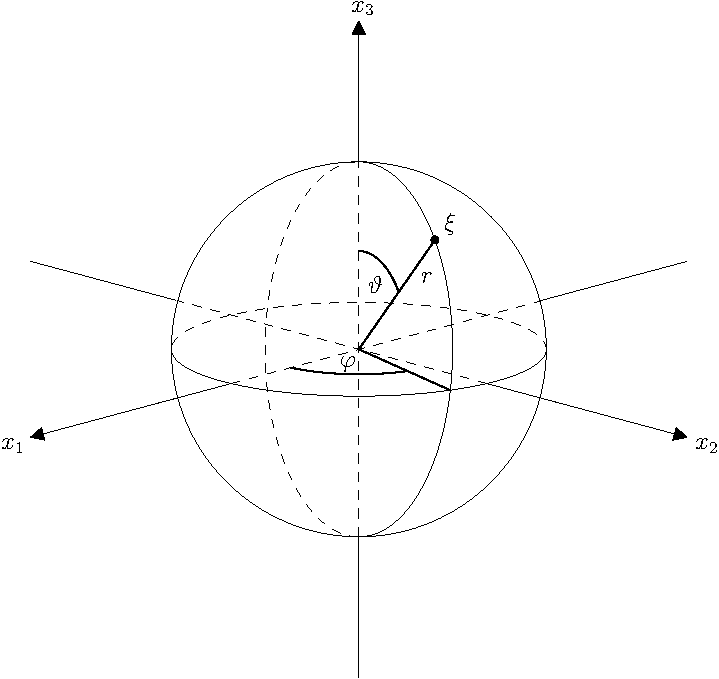
\includegraphics[width=0.45\textwidth]{sphere}}
 For consistency with the other modules and the conventions used there, we also use {\em swapped\/} {\em scaled\/} {\em spherical\/} {\em coordinates\/} $x_1 := \frac{\varphi}{2\pi}$, $x_2 := \frac{\vartheta}{2\pi}$ and identify a point from $\mathbb{S}^2$ with the vector $\mathbf{x} := \left(x_1,x_2\right) \in [-\frac{1}{2}, \frac{1}{2}) \times [0,\frac{1}{2}]$.\hypertarget{group__nfsft_lp}{}\subsubsection{Legendre Polynomials}\label{group__nfsft_lp}
The {\em Legendre\/} {\em polynomials\/} $P_k : [-1,1] \rightarrow \mathbb{R}$, $k \in \mathbb{N}_{0}$ as {\em classical\/} {\em orthogonal\/} {\em polynomials\/} are given by their corresponding {\em Rodrigues\/} {\em formula\/} \[ P_k(t) := \frac{1}{2^k k!} \frac{\text{d}^k}{\text{d} t^k} \left(t^2-1\right)^k. \] The corresponding three-term recurrence relation is \[ (k+1)P_{k+1}(t) = (2k+1) x P_{k}(t) - k P_{k-1}(t) \quad (k \in \mathbb{N}_0). \] With \[ \left< f,g \right>_{\text{L}^2\left([-1,1]\right)} := \int_{-1}^{1} f(t) g(t) \text{d} t \] being the usual $\text{L}^2\left([-1,1]\right)$ inner product, the Legendre polynomials obey the orthogonality condition \[ \left< P_k,P_l \right>_{\text{L}^2\left([-1,1]\right)} = \frac{2}{2k+1} \delta_{k,l}. \]

\begin{Desc}
\item[Remarks:]The normalisation constant $ c_k := \sqrt{\frac{2k+1}{2}}$ renders the scaled Legendre polynomials $c_k P_k$ orthonormal with respect to the induced $\text{L}^2\left([-1,1]\right)$ norm \[ \|f\|_{\text{L}^2\left([-1,1]\right)} := \left(<f,f>_{\text{L}^2\left([-1,1]\right)}\right)^{1/2} = \left(\int_{-1}^{1} |f(t)|^2 \; \text{d} t\right)^{1/2}. \]\end{Desc}
\hypertarget{group__nfsft_alf}{}\subsubsection{Associated Legendre Functions}\label{group__nfsft_alf}
The {\em associated\/} {\em Legendre\/} {\em functions\/} $P_k^n : [-1,1] \rightarrow \mathbb{R} $, $n \in \mathbb{N}_0$, $k \ge n$ are defined by \[ P_k^n(t) := \left(\frac{(k-n)!}{(k+n)!}\right)^{1/2} \left(1-t^2\right)^{n/2} \frac{\text{d}^n}{\text{d} t^n} P_k(t). \] For $n = 0$, they coincide with the Legendre polynomials, i.e. $P_k^0 = P_k$. The associated Legendre functions obey the three-term recurrence relation \[ P_{k+1}^n(t) = v_{k}^n t P_k^n(t) + w_{k}^n P_{k-1}^n(t) \quad (k \ge n), \] with $P_{n-1}^n(t) := 0$, $P_{n}^n(t) := \frac{\sqrt{(2n)!}}{2^n n!} \left(1-t^2\right)^{n/2}$, and \[ v_{k}^n := \frac{2k+1}{((k-n+1)(k+n+1))^{1/2}}\; ,\qquad w_{k}^n := - \frac{((k-n)(k+n))^{1/2}}{((k-n+1)(k+n+1))^{1/2}}. \] For fixed $n$, the set $\left\{P_k^n:\: k \ge n\right\}$ forms a complete set of orthogonal functions in $\text{L}^2\left([-1,1]\right)$ with \[ \left< P_k^n,P_l^n \right>_{\text{L}^2\left([-1,1]\right)} = \frac{2}{2k+1} \delta_{k,l} \quad (0 \le n \le k,l). \]

\begin{Desc}
\item[Remarks:]The normalisation constant $ c_k = \sqrt{\frac{2k+1}{2}}$ renders the scaled associated Legendre functions $c_k P_k^n$ orthonormal with respect to the induced $\text{L}^2\left([-1,1]\right)$ norm \[ \|f\|_{\text{L}^2\left([-1,1]\right)} := \left(<f,f>_{\text{L}^2\left([-1,1]\right)}\right)^{1/2} = \left(\int_{-1}^{1} |f(t)|^2 \; \text{d} t\right)^{1/2}. \]\end{Desc}
\hypertarget{group__nfsft_sh}{}\subsubsection{Spherical Harmonics}\label{group__nfsft_sh}
The standard orthogonal basis of spherical harmonics for $\text{L}^2 \left(\mathbb{S}^2\right)$ with yet unnormalised basis functions $\tilde{Y}_k^n : \mathbb{S}^2 \rightarrow \mathbb{C}$ is given by \[ \tilde{Y}_k^n(\vartheta,\varphi) := P_k^{|n|}(\cos\vartheta) \mathrm{e}^{\mathrm{i} n \varphi} \] with the usual $\text{L}^2\left(\mathbb{S}^2\right)$ inner product \[ \left< f,g \right>_{\mathrm{L}^2\left(\mathbb{S}^2\right)} := \int_{\mathbb{S}^2} f(\vartheta,\varphi) \overline{g(\vartheta,\varphi)} \: \mathrm{d} \mathbf{\xi} := \int_{-\pi}^{\pi} \int_{0}^{\pi} f(\vartheta,\varphi) \overline{g(\vartheta,\varphi)} \sin \vartheta \; \mathrm{d} \vartheta \; \mathrm{d} \varphi. \] The normalisation constant $c_k^n := \sqrt{\frac{2k+1}{4\pi}}$ renders the scaled basis functions \[ Y_k^n(\vartheta,\varphi) := c_k^n P_k^{|n|}(\cos\vartheta) \mathrm{e}^{\mathrm{i} n \varphi} \] orthonormal with respect to the induced $\text{L}^2\left(\mathbb{S}^2 \right)$ norm \[ \|f\|_{\text{L}^2\left(\mathbb{S}^2\right)} = \left(<f,f>_{\text{L}^2\left(\mathbb{S}^2\right)}\right)^{1/2} = \left(\int_{-\pi}^{\pi} \int_{0}^{\pi} |f(\vartheta,\varphi)|^2 \sin \vartheta \; \mathrm{d} \vartheta \; \mathrm{d} \varphi\right)^{1/2}. \] A function $f \in \mathrm{L}^2\left(\mathbb{S}^2\right)$ has the orthogonal expansion \[ f = \sum_{k=0}^{\infty} \sum_{n=-k}^{k} \hat{f}(k,n) Y_k^n, \] where the coefficients $\hat{f}(k,n) := \left< f, Y_k^{n} \right>_{\mathrm{L}^2\left(\mathbb{S}^2\right)}$ are the {\em spherical\/} {\em Fourier\/} {\em coefficients\/} and the equivalence is understood in the $\mathrm{L}^2$-sense.\hypertarget{group__nfsft_nfsfts}{}\subsection{Nonuniform Fast Spherical Fourier Transforms}\label{group__nfsft_nfsfts}
This section describes the input and output relation of the spherical Fourier transform algorithms and the layout of the corresponding plan structure.\hypertarget{group__nfsft_ndsft}{}\subsubsection{Nonuniform Discrete Spherical Fourier Transform}\label{group__nfsft_ndsft}
The {\em nonuniform\/} {\em discrete\/} {\em spherical\/} {\em Fourier\/} {\em transform\/} ({\em NDSFT\/}) is defined as follows: \[ \begin{array}{rcl} \text{\textbf{Input}} & : & \text{coefficients } \hat{f}(k,n) \in \mathbb{C} \text{ for } k=0,\ldots,N,\;n=-k, \ldots,k,\; N \in \mathbb{N}_0,\\[1ex] & & \text{arbitrary nodes } \mathbf{x}(m) \in [-\frac{1}{2},\frac{1}{2}] \times [0,\frac{1}{2}] \text{ for } m=0,\ldots,M-1, M \in \mathbb{N}. \\[1ex] \text{\textbf{Task}} & : & \text{evaluate } f(m) := f\left( \mathbf{x}(m)\right) = \sum_{k=0}^N \sum_{n=-k}^k \hat{f}_k^n Y_k^n\left(\mathbf{x}(m)\right) \text{ for } m=0,\ldots,M-1. \\[1ex] \text{\textbf{Output}} & : & \text{coefficients } f(m) \in \mathbb{C} \text{ for } m=0,\ldots,M-1.\\ \end{array} \]\hypertarget{group__nfsft_andsft}{}\subsubsection{Adjoint Nonuniform Discrete Spherical Fourier Transform}\label{group__nfsft_andsft}
The {\em adjoint\/} {\em nonuniform\/} {\em discrete\/} {\em spherical\/} {\em Fourier\/} {\em transform\/} ({\em adjoint\/} {\em NDSFT\/}) is defined as follows: \[ \begin{array}{rcl} \text{\textbf{Input}} & : & \text{coefficients } f(m) \in \mathbb{C} \text{ for } m=0,\ldots,M-1, M \in \mathbb{N},\\ & & \text{arbitrary nodes } \mathbf{x}(m) \in [-\frac{1}{2},\frac{1}{2}] \times [0,\frac{1}{2}] \text{ for } m=0,\ldots,M-1, N \in \mathbb{N}_0.\\[1ex] \text{\textbf{Task}} & : & \text{evaluate } \hat{f}(k,n) := \sum_{m=0}^{M-1} f(m) \overline{Y_k^n\left(\mathbf{x}(m)\right)}cd Do \text{ for } k=0,\ldots,N,\;n=-k,\ldots,k.\\[1ex] \text{\textbf{Output}} & : & \text{coefficients } \hat{f}(k,n) \in \mathbb{C} \text{ for } k=0,\ldots,N,\;n=-k,\ldots,k.\\[1ex] \end{array} \]\hypertarget{group__nfsft_dl}{}\subsubsection{Data Layout}\label{group__nfsft_dl}
This section describes the public layout of the \hyperlink{structnfsft__plan}{nfsft\_\-plan} structure which contains all data for the computation of the aforementioned spherical Fourier transforms. The structure contains private (no read or write allowed), public read-only (only read access permitted), and public read-write (read and write access allowed) members. In the following, we indicate read and write access by {\tt read} and {\tt write}. The public members are structured as follows: \begin{itemize}
\item {\tt N\_\-total} ({\tt read}) The total number of components in {\tt f\_\-hat}. If the bandwidth is $N \in \mathbb{N}_0$, the total number of components in {\tt f\_\-hat} is {\tt N\_\-total} $ = (2N+2)^2$. \item {\tt M\_\-total} ({\tt read}) the total number of samples $M$ \item {\tt f\_\-hat} ({\tt read-write}) The flattened array of spherical Fourier coefficents. The array has length $(2N+2)^2$ such that valid indices $i \in \mathbb{N}_0$ for array access {\tt f\_\-hat} {\tt }\mbox{[} $i$ {\tt }\mbox{]} are $i=0,1,\ldots,(2N+2)^2-1$. However, only read and write access to indices corresponding to spherical Fourier coefficients $\hat{f}(k,n)$ is defined. The index $i$ corresponding to the spherical Fourier coefficient $\hat{f}(k,n)$ with $0 \le k \le M$, $-k \le n \le k$ is $i = (N+2)(N-n+1)+N+k+1$. For convenience, the helper macro \hyperlink{group__nfsft_ga40}{NFSFT\_\-INDEX(k,n)} provides the necessary index calculations such that one can write {\tt f\_\-hat}\mbox{[} {\tt NFSFT\_\-INDEX}($k,n${\tt })\mbox{]} {\tt =} {\tt }... to access the component corresponding to $\hat{f}(k,n)$. The data layout is due to implementation details. \item {\tt f} ({\tt read-write}) the array of coefficients $f(m)$ for $m=0,\ldots,M-1$ such that {\tt f}\mbox{[}$m${\tt }\mbox{]} = $f(m)$ \item {\tt N} ({\tt read}) the bandwidth $N \in \mathbb{N}_0$ \item {\tt x} the array of nodes $\mathbf{x}(m) \in [-\frac{1}{2},\frac{1}{2}] \times [0,\frac{1}{2}]$ for $m = 0, \ldots,M-1$ such that {\tt f}\mbox{[}$2m${\tt }\mbox{]} = $x_1$ and {\tt f}\mbox{[}$2m+1${\tt }\mbox{]} = $x_2$\end{itemize}
\hypertarget{group__nfsft_gtn}{}\subsubsection{Good to know...}\label{group__nfsft_gtn}
When using the routines of this module you should bear in mind the following: \begin{itemize}
\item The bandwidth $N_{\text{max}}$ up to which precomputation is performed is always chosen as the next power of two with respect to the specified maximum bandwidth. \item By default, the NDSFT transforms (see \hyperlink{group__nfsft_ga6}{ndsft\_\-trafo}, \hyperlink{group__nfsft_ga8}{nfsft\_\-trafo}) are allowed to destroy the input {\tt f\_\-hat} while the input {\tt x} is preserved. On the contrary, the adjoint NDSFT transforms (see \hyperlink{group__nfsft_ga7}{ndsft\_\-adjoint}, \hyperlink{group__nfsft_ga9}{nfsft\_\-adjoint}) do not destroy the input {\tt f} and {\tt x} by default. The desired behaviour can be assured by using the \hyperlink{group__nfsft_ga31}{NFSFT\_\-PRESERVE\_\-F\_\-HAT}, \hyperlink{group__nfsft_ga32}{NFSFT\_\-PRESERVE\_\-X}, \hyperlink{group__nfsft_ga33}{NFSFT\_\-PRESERVE\_\-F} and \hyperlink{group__nfsft_ga34}{NFSFT\_\-DESTROY\_\-F\_\-HAT}, \hyperlink{group__nfsft_ga35}{NFSFT\_\-DESTROY\_\-X}, \hyperlink{group__nfsft_ga36}{NFSFT\_\-DESTROY\_\-F} flags. \end{itemize}


\subsection{Define Documentation}
\hypertarget{group__nfsft_ga25}{
\index{nfsft@{nfsft}!NFSFT_NORMALIZED@{NFSFT\_\-NORMALIZED}}
\index{NFSFT_NORMALIZED@{NFSFT\_\-NORMALIZED}!nfsft@{nfsft}}
\subsubsection[NFSFT\_\-NORMALIZED]{\setlength{\rightskip}{0pt plus 5cm}\#define NFSFT\_\-NORMALIZED~(1U $<$$<$ 0)}}
\label{group__nfsft_ga25}


By default, all computations are performed with respect to the unnormalized basis functions \[ \tilde{Y}_k^n(\vartheta,\varphi) = P_k^{|n|}(\cos\vartheta) \mathrm{e}^{\mathrm{i} n \varphi}. \] If this flag is set, all computations are carried out using the $L_2$- normalized basis functions \[ Y_k^n(\vartheta,\varphi) = \sqrt{\frac{2k+1}{4\pi}} P_k^{|n|}(\cos\vartheta) \mathrm{e}^{\mathrm{i} n \varphi}. \]. 

\begin{Desc}
\item[See also:]\hyperlink{group__nfsft_ga1}{nfsft\_\-init} 

\hyperlink{group__nfsft_ga2}{nfsft\_\-init\_\-advanced} 

\hyperlink{group__nfsft_ga3}{nfsft\_\-init\_\-guru} \end{Desc}
\begin{Desc}
\item[Author:]Jens Keiner \end{Desc}


Definition at line 1718 of file nfft3.h.

Referenced by main(), ndsft\_\-adjoint(), ndsft\_\-trafo(), nfsft\_\-adjoint(), and nfsft\_\-trafo().\hypertarget{group__nfsft_ga26}{
\index{nfsft@{nfsft}!NFSFT_USE_NDFT@{NFSFT\_\-USE\_\-NDFT}}
\index{NFSFT_USE_NDFT@{NFSFT\_\-USE\_\-NDFT}!nfsft@{nfsft}}
\subsubsection[NFSFT\_\-USE\_\-NDFT]{\setlength{\rightskip}{0pt plus 5cm}\#define NFSFT\_\-USE\_\-NDFT~(1U $<$$<$ 1)}}
\label{group__nfsft_ga26}


If this flag is set, the fast NFSFT algorithms (see \hyperlink{group__nfsft_ga8}{nfsft\_\-trafo}, \hyperlink{group__nfsft_ga9}{nfsft\_\-adjoint}) will use internally the exact but usually slower direct NDFT algorithm in favor of fast but approximative NFFT algorithm. 

\begin{Desc}
\item[See also:]\hyperlink{group__nfsft_ga1}{nfsft\_\-init} 

\hyperlink{group__nfsft_ga2}{nfsft\_\-init\_\-advanced} 

\hyperlink{group__nfsft_ga3}{nfsft\_\-init\_\-guru} \end{Desc}
\begin{Desc}
\item[Author:]Jens Keiner \end{Desc}


Definition at line 1730 of file nfft3.h.

Referenced by main(), nfsft\_\-adjoint(), and nfsft\_\-trafo().\hypertarget{group__nfsft_ga27}{
\index{nfsft@{nfsft}!NFSFT_USE_DPT@{NFSFT\_\-USE\_\-DPT}}
\index{NFSFT_USE_DPT@{NFSFT\_\-USE\_\-DPT}!nfsft@{nfsft}}
\subsubsection[NFSFT\_\-USE\_\-DPT]{\setlength{\rightskip}{0pt plus 5cm}\#define NFSFT\_\-USE\_\-DPT~(1U $<$$<$ 2)}}
\label{group__nfsft_ga27}


If this flag is set, the fast NFSFT algorithms (see \hyperlink{group__nfsft_ga8}{nfsft\_\-trafo}, \hyperlink{group__nfsft_ga9}{nfsft\_\-adjoint}) will use internally the usually slower direct DPT algorithm in favor of the fast FPT algorithm. 

\begin{Desc}
\item[See also:]\hyperlink{group__nfsft_ga1}{nfsft\_\-init} 

\hyperlink{group__nfsft_ga2}{nfsft\_\-init\_\-advanced} 

\hyperlink{group__nfsft_ga3}{nfsft\_\-init\_\-guru} \end{Desc}
\begin{Desc}
\item[Author:]Jens Keiner \end{Desc}
\begin{Desc}
\item[Warning:]This feature is not implemented yet! \end{Desc}


Definition at line 1743 of file nfft3.h.

Referenced by main(), nfsft\_\-adjoint(), and nfsft\_\-trafo().\hypertarget{group__nfsft_ga28}{
\index{nfsft@{nfsft}!NFSFT_MALLOC_X@{NFSFT\_\-MALLOC\_\-X}}
\index{NFSFT_MALLOC_X@{NFSFT\_\-MALLOC\_\-X}!nfsft@{nfsft}}
\subsubsection[NFSFT\_\-MALLOC\_\-X]{\setlength{\rightskip}{0pt plus 5cm}\#define NFSFT\_\-MALLOC\_\-X~(1U $<$$<$ 3)}}
\label{group__nfsft_ga28}


If this flag is set, the init methods (see \hyperlink{group__nfsft_ga1}{nfsft\_\-init} , \hyperlink{group__nfsft_ga2}{nfsft\_\-init\_\-advanced} , and \hyperlink{group__nfsft_ga3}{nfsft\_\-init\_\-guru}) will allocate memory and the method \hyperlink{group__nfsft_ga10}{nfsft\_\-finalize} will free the array {\tt x} for you. 

Otherwise, you have to assure by yourself that {\tt x} points to an array of proper size before excuting a transform and you are responsible for freeing the corresponding memory before program termination.

\begin{Desc}
\item[See also:]\hyperlink{group__nfsft_ga1}{nfsft\_\-init} 

\hyperlink{group__nfsft_ga2}{nfsft\_\-init\_\-advanced} 

\hyperlink{group__nfsft_ga3}{nfsft\_\-init\_\-guru} \end{Desc}
\begin{Desc}
\item[Author:]Jens Keiner \end{Desc}


Definition at line 1758 of file nfft3.h.

Referenced by main(), nfsft\_\-finalize(), nfsft\_\-init(), and nfsft\_\-init\_\-guru().\hypertarget{group__nfsft_ga29}{
\index{nfsft@{nfsft}!NFSFT_MALLOC_F_HAT@{NFSFT\_\-MALLOC\_\-F\_\-HAT}}
\index{NFSFT_MALLOC_F_HAT@{NFSFT\_\-MALLOC\_\-F\_\-HAT}!nfsft@{nfsft}}
\subsubsection[NFSFT\_\-MALLOC\_\-F\_\-HAT]{\setlength{\rightskip}{0pt plus 5cm}\#define NFSFT\_\-MALLOC\_\-F\_\-HAT~(1U $<$$<$ 5)}}
\label{group__nfsft_ga29}


If this flag is set, the init methods (see \hyperlink{group__nfsft_ga1}{nfsft\_\-init} , \hyperlink{group__nfsft_ga2}{nfsft\_\-init\_\-advanced} , and \hyperlink{group__nfsft_ga3}{nfsft\_\-init\_\-guru}) will allocate memory and the method \hyperlink{group__nfsft_ga10}{nfsft\_\-finalize} will free the array {\tt f\_\-hat} for you. 

Otherwise, you have to assure by yourself that {\tt f\_\-hat} points to an array of proper size before excuting a transform and you are responsible for freeing the corresponding memory before program termination.

\begin{Desc}
\item[See also:]\hyperlink{group__nfsft_ga1}{nfsft\_\-init} 

\hyperlink{group__nfsft_ga2}{nfsft\_\-init\_\-advanced} 

\hyperlink{group__nfsft_ga3}{nfsft\_\-init\_\-guru} \end{Desc}
\begin{Desc}
\item[Author:]Jens Keiner \end{Desc}


Definition at line 1773 of file nfft3.h.

Referenced by main(), nfsft\_\-finalize(), nfsft\_\-init(), and nfsft\_\-init\_\-guru().\hypertarget{group__nfsft_ga30}{
\index{nfsft@{nfsft}!NFSFT_MALLOC_F@{NFSFT\_\-MALLOC\_\-F}}
\index{NFSFT_MALLOC_F@{NFSFT\_\-MALLOC\_\-F}!nfsft@{nfsft}}
\subsubsection[NFSFT\_\-MALLOC\_\-F]{\setlength{\rightskip}{0pt plus 5cm}\#define NFSFT\_\-MALLOC\_\-F~(1U $<$$<$ 6)}}
\label{group__nfsft_ga30}


If this flag is set, the init methods (see \hyperlink{group__nfsft_ga1}{nfsft\_\-init} , \hyperlink{group__nfsft_ga2}{nfsft\_\-init\_\-advanced} , and \hyperlink{group__nfsft_ga3}{nfsft\_\-init\_\-guru}) will allocate memory and the method \hyperlink{group__nfsft_ga10}{nfsft\_\-finalize} will free the array {\tt f} for you. 

Otherwise, you have to assure by yourself that {\tt f} points to an array of proper size before excuting a transform and you are responsible for freeing the corresponding memory before program termination.

\begin{Desc}
\item[See also:]\hyperlink{group__nfsft_ga1}{nfsft\_\-init} 

\hyperlink{group__nfsft_ga2}{nfsft\_\-init\_\-advanced} 

\hyperlink{group__nfsft_ga3}{nfsft\_\-init\_\-guru} \end{Desc}
\begin{Desc}
\item[Author:]Jens Keiner \end{Desc}


Definition at line 1788 of file nfft3.h.

Referenced by main(), nfsft\_\-finalize(), nfsft\_\-init(), and nfsft\_\-init\_\-guru().\hypertarget{group__nfsft_ga31}{
\index{nfsft@{nfsft}!NFSFT_PRESERVE_F_HAT@{NFSFT\_\-PRESERVE\_\-F\_\-HAT}}
\index{NFSFT_PRESERVE_F_HAT@{NFSFT\_\-PRESERVE\_\-F\_\-HAT}!nfsft@{nfsft}}
\subsubsection[NFSFT\_\-PRESERVE\_\-F\_\-HAT]{\setlength{\rightskip}{0pt plus 5cm}\#define NFSFT\_\-PRESERVE\_\-F\_\-HAT~(1U $<$$<$ 7)}}
\label{group__nfsft_ga31}


If this flag is set, it is guaranteed that during an execution of \hyperlink{group__nfsft_ga6}{ndsft\_\-trafo} or \hyperlink{group__nfsft_ga8}{nfsft\_\-trafo} the content of {\tt f\_\-hat} remains unchanged. 

\begin{Desc}
\item[See also:]\hyperlink{group__nfsft_ga1}{nfsft\_\-init} 

\hyperlink{group__nfsft_ga2}{nfsft\_\-init\_\-advanced} 

\hyperlink{group__nfsft_ga3}{nfsft\_\-init\_\-guru} \end{Desc}
\begin{Desc}
\item[Author:]Jens Keiner \end{Desc}


Definition at line 1800 of file nfft3.h.

Referenced by ndsft\_\-trafo(), nfsft\_\-finalize(), nfsft\_\-init\_\-guru(), and nfsft\_\-trafo().\hypertarget{group__nfsft_ga32}{
\index{nfsft@{nfsft}!NFSFT_PRESERVE_X@{NFSFT\_\-PRESERVE\_\-X}}
\index{NFSFT_PRESERVE_X@{NFSFT\_\-PRESERVE\_\-X}!nfsft@{nfsft}}
\subsubsection[NFSFT\_\-PRESERVE\_\-X]{\setlength{\rightskip}{0pt plus 5cm}\#define NFSFT\_\-PRESERVE\_\-X~(1U $<$$<$ 8)}}
\label{group__nfsft_ga32}


If this flag is set, it is guaranteed that during an execution of \hyperlink{group__nfsft_ga6}{ndsft\_\-trafo}, \hyperlink{group__nfsft_ga8}{nfsft\_\-trafo} or \hyperlink{group__nfsft_ga7}{ndsft\_\-adjoint}, \hyperlink{group__nfsft_ga9}{nfsft\_\-adjoint} the content of {\tt x} remains unchanged. 

\begin{Desc}
\item[See also:]\hyperlink{group__nfsft_ga1}{nfsft\_\-init} 

\hyperlink{group__nfsft_ga2}{nfsft\_\-init\_\-advanced} 

\hyperlink{group__nfsft_ga3}{nfsft\_\-init\_\-guru} \end{Desc}
\begin{Desc}
\item[Author:]Jens Keiner \end{Desc}


Definition at line 1813 of file nfft3.h.\hypertarget{group__nfsft_ga33}{
\index{nfsft@{nfsft}!NFSFT_PRESERVE_F@{NFSFT\_\-PRESERVE\_\-F}}
\index{NFSFT_PRESERVE_F@{NFSFT\_\-PRESERVE\_\-F}!nfsft@{nfsft}}
\subsubsection[NFSFT\_\-PRESERVE\_\-F]{\setlength{\rightskip}{0pt plus 5cm}\#define NFSFT\_\-PRESERVE\_\-F~(1U $<$$<$ 9)}}
\label{group__nfsft_ga33}


If this flag is set, it is guaranteed that during an execution of \hyperlink{group__nfsft_ga7}{ndsft\_\-adjoint} or \hyperlink{group__nfsft_ga9}{nfsft\_\-adjoint} the content of {\tt f} remains unchanged. 

\begin{Desc}
\item[See also:]\hyperlink{group__nfsft_ga1}{nfsft\_\-init} 

\hyperlink{group__nfsft_ga2}{nfsft\_\-init\_\-advanced} 

\hyperlink{group__nfsft_ga3}{nfsft\_\-init\_\-guru} \end{Desc}
\begin{Desc}
\item[Author:]Jens Keiner \end{Desc}


Definition at line 1825 of file nfft3.h.\hypertarget{group__nfsft_ga34}{
\index{nfsft@{nfsft}!NFSFT_DESTROY_F_HAT@{NFSFT\_\-DESTROY\_\-F\_\-HAT}}
\index{NFSFT_DESTROY_F_HAT@{NFSFT\_\-DESTROY\_\-F\_\-HAT}!nfsft@{nfsft}}
\subsubsection[NFSFT\_\-DESTROY\_\-F\_\-HAT]{\setlength{\rightskip}{0pt plus 5cm}\#define NFSFT\_\-DESTROY\_\-F\_\-HAT~(1U $<$$<$ 10)}}
\label{group__nfsft_ga34}


If this flag is set, it is explicitely allowed that during an execution of \hyperlink{group__nfsft_ga6}{ndsft\_\-trafo} or \hyperlink{group__nfsft_ga8}{nfsft\_\-trafo} the content of {\tt f\_\-hat} may be changed. 

\begin{Desc}
\item[See also:]\hyperlink{group__nfsft_ga1}{nfsft\_\-init} 

\hyperlink{group__nfsft_ga2}{nfsft\_\-init\_\-advanced} 

\hyperlink{group__nfsft_ga3}{nfsft\_\-init\_\-guru} \end{Desc}
\begin{Desc}
\item[Author:]Jens Keiner \end{Desc}


Definition at line 1836 of file nfft3.h.\hypertarget{group__nfsft_ga35}{
\index{nfsft@{nfsft}!NFSFT_DESTROY_X@{NFSFT\_\-DESTROY\_\-X}}
\index{NFSFT_DESTROY_X@{NFSFT\_\-DESTROY\_\-X}!nfsft@{nfsft}}
\subsubsection[NFSFT\_\-DESTROY\_\-X]{\setlength{\rightskip}{0pt plus 5cm}\#define NFSFT\_\-DESTROY\_\-X~(1U $<$$<$ 11)}}
\label{group__nfsft_ga35}


If this flag is set, it is explicitely allowed that during an execution of \hyperlink{group__nfsft_ga6}{ndsft\_\-trafo}, \hyperlink{group__nfsft_ga8}{nfsft\_\-trafo} or \hyperlink{group__nfsft_ga7}{ndsft\_\-adjoint}, \hyperlink{group__nfsft_ga9}{nfsft\_\-adjoint} the content of {\tt x} may be changed. 

\begin{Desc}
\item[See also:]\hyperlink{group__nfsft_ga1}{nfsft\_\-init} 

\hyperlink{group__nfsft_ga2}{nfsft\_\-init\_\-advanced} 

\hyperlink{group__nfsft_ga3}{nfsft\_\-init\_\-guru} \end{Desc}
\begin{Desc}
\item[Author:]Jens Keiner \end{Desc}


Definition at line 1848 of file nfft3.h.\hypertarget{group__nfsft_ga36}{
\index{nfsft@{nfsft}!NFSFT_DESTROY_F@{NFSFT\_\-DESTROY\_\-F}}
\index{NFSFT_DESTROY_F@{NFSFT\_\-DESTROY\_\-F}!nfsft@{nfsft}}
\subsubsection[NFSFT\_\-DESTROY\_\-F]{\setlength{\rightskip}{0pt plus 5cm}\#define NFSFT\_\-DESTROY\_\-F~(1U $<$$<$ 12)}}
\label{group__nfsft_ga36}


If this flag is set, it is explicitely allowed that during an execution of \hyperlink{group__nfsft_ga7}{ndsft\_\-adjoint} or \hyperlink{group__nfsft_ga9}{nfsft\_\-adjoint} the content of {\tt f} may be changed. 

\begin{Desc}
\item[See also:]\hyperlink{group__nfsft_ga1}{nfsft\_\-init} 

\hyperlink{group__nfsft_ga2}{nfsft\_\-init\_\-advanced} 

\hyperlink{group__nfsft_ga3}{nfsft\_\-init\_\-guru} \end{Desc}
\begin{Desc}
\item[Author:]Jens Keiner \end{Desc}


Definition at line 1859 of file nfft3.h.\hypertarget{group__nfsft_ga37}{
\index{nfsft@{nfsft}!NFSFT_NO_DIRECT_ALGORITHM@{NFSFT\_\-NO\_\-DIRECT\_\-ALGORITHM}}
\index{NFSFT_NO_DIRECT_ALGORITHM@{NFSFT\_\-NO\_\-DIRECT\_\-ALGORITHM}!nfsft@{nfsft}}
\subsubsection[NFSFT\_\-NO\_\-DIRECT\_\-ALGORITHM]{\setlength{\rightskip}{0pt plus 5cm}\#define NFSFT\_\-NO\_\-DIRECT\_\-ALGORITHM~(1U $<$$<$ 13)}}
\label{group__nfsft_ga37}


If this flag is set, the transforms \hyperlink{group__nfsft_ga6}{ndsft\_\-trafo} and \hyperlink{group__nfsft_ga7}{ndsft\_\-adjoint} do not work. 

Setting this flag saves some memory for precomputed data.

\begin{Desc}
\item[See also:]\hyperlink{group__nfsft_ga4}{nfsft\_\-precompute} 

\hyperlink{group__nfsft_ga6}{ndsft\_\-trafo} 

\hyperlink{group__nfsft_ga7}{ndsft\_\-adjoint} \end{Desc}
\begin{Desc}
\item[Author:]Jens Keiner \end{Desc}


Definition at line 1872 of file nfft3.h.

Referenced by ndsft\_\-adjoint(), ndsft\_\-trafo(), nfsft\_\-forget(), and nfsft\_\-precompute().\hypertarget{group__nfsft_ga38}{
\index{nfsft@{nfsft}!NFSFT_NO_FAST_ALGORITHM@{NFSFT\_\-NO\_\-FAST\_\-ALGORITHM}}
\index{NFSFT_NO_FAST_ALGORITHM@{NFSFT\_\-NO\_\-FAST\_\-ALGORITHM}!nfsft@{nfsft}}
\subsubsection[NFSFT\_\-NO\_\-FAST\_\-ALGORITHM]{\setlength{\rightskip}{0pt plus 5cm}\#define NFSFT\_\-NO\_\-FAST\_\-ALGORITHM~(1U $<$$<$ 14)}}
\label{group__nfsft_ga38}


If this flag is set, the transforms \hyperlink{group__nfsft_ga8}{nfsft\_\-trafo} and \hyperlink{group__nfsft_ga9}{nfsft\_\-adjoint} do not work. 

Setting this flag saves memory for precomputed data.

\begin{Desc}
\item[See also:]\hyperlink{group__nfsft_ga4}{nfsft\_\-precompute} 

\hyperlink{group__nfsft_ga8}{nfsft\_\-trafo} 

\hyperlink{group__nfsft_ga9}{nfsft\_\-adjoint} \end{Desc}
\begin{Desc}
\item[Author:]Jens Keiner \end{Desc}


Definition at line 1883 of file nfft3.h.

Referenced by main(), nfsft\_\-adjoint(), nfsft\_\-forget(), nfsft\_\-init\_\-guru(), nfsft\_\-precompute(), and nfsft\_\-trafo().\hypertarget{group__nfsft_ga39}{
\index{nfsft@{nfsft}!NFSFT_ZERO_F_HAT@{NFSFT\_\-ZERO\_\-F\_\-HAT}}
\index{NFSFT_ZERO_F_HAT@{NFSFT\_\-ZERO\_\-F\_\-HAT}!nfsft@{nfsft}}
\subsubsection[NFSFT\_\-ZERO\_\-F\_\-HAT]{\setlength{\rightskip}{0pt plus 5cm}\#define NFSFT\_\-ZERO\_\-F\_\-HAT~(1U $<$$<$ 16)}}
\label{group__nfsft_ga39}


If this flag is set, the transforms \hyperlink{group__nfsft_ga9}{nfsft\_\-adjoint} and \hyperlink{group__nfsft_ga7}{ndsft\_\-adjoint} set all unused entries in {\tt f\_\-hat} not corresponding to spherical Fourier coefficients to zero. 

\begin{Desc}
\item[Author:]Jens Keiner \end{Desc}


Definition at line 1892 of file nfft3.h.

Referenced by main(), ndsft\_\-adjoint(), and nfsft\_\-adjoint().\hypertarget{group__nfsft_ga46}{
\index{nfsft@{nfsft}!NFSFT_DEFAULT_NFFT_CUTOFF@{NFSFT\_\-DEFAULT\_\-NFFT\_\-CUTOFF}}
\index{NFSFT_DEFAULT_NFFT_CUTOFF@{NFSFT\_\-DEFAULT\_\-NFFT\_\-CUTOFF}!nfsft@{nfsft}}
\subsubsection[NFSFT\_\-DEFAULT\_\-NFFT\_\-CUTOFF]{\setlength{\rightskip}{0pt plus 5cm}\#define NFSFT\_\-DEFAULT\_\-NFFT\_\-CUTOFF~6}}
\label{group__nfsft_ga46}


The default NFFT cutoff parameter. 

\begin{Desc}
\item[Author:]Jens Keiner \end{Desc}


Definition at line 34 of file nfsft.c.

Referenced by nfsft\_\-init\_\-advanced().\hypertarget{group__nfsft_ga47}{
\index{nfsft@{nfsft}!NFSFT_DEFAULT_THRESHOLD@{NFSFT\_\-DEFAULT\_\-THRESHOLD}}
\index{NFSFT_DEFAULT_THRESHOLD@{NFSFT\_\-DEFAULT\_\-THRESHOLD}!nfsft@{nfsft}}
\subsubsection[NFSFT\_\-DEFAULT\_\-THRESHOLD]{\setlength{\rightskip}{0pt plus 5cm}\#define NFSFT\_\-DEFAULT\_\-THRESHOLD~1000}}
\label{group__nfsft_ga47}


The default threshold for the FPT. 

\begin{Desc}
\item[Author:]Jens Keiner \end{Desc}


Definition at line 41 of file nfsft.c.\hypertarget{group__nfsft_ga48}{
\index{nfsft@{nfsft}!NFSFT_BREAK_EVEN@{NFSFT\_\-BREAK\_\-EVEN}}
\index{NFSFT_BREAK_EVEN@{NFSFT\_\-BREAK\_\-EVEN}!nfsft@{nfsft}}
\subsubsection[NFSFT\_\-BREAK\_\-EVEN]{\setlength{\rightskip}{0pt plus 5cm}\#define NFSFT\_\-BREAK\_\-EVEN~5}}
\label{group__nfsft_ga48}


The break-even bandwidth $N \in \mathbb{N}_0$. 

\begin{Desc}
\item[Author:]Jens Keiner \end{Desc}


Definition at line 48 of file nfsft.c.

Referenced by nfsft\_\-adjoint(), nfsft\_\-forget(), nfsft\_\-precompute(), and nfsft\_\-trafo().

\subsection{Function Documentation}
\hypertarget{group__nfsft_ga1}{
\index{nfsft@{nfsft}!nfsft_init@{nfsft\_\-init}}
\index{nfsft_init@{nfsft\_\-init}!nfsft@{nfsft}}
\subsubsection[nfsft\_\-init]{\setlength{\rightskip}{0pt plus 5cm}void nfsft\_\-init (\hyperlink{structnfsft__plan}{nfsft\_\-plan} $\ast$ {\em plan}, int {\em N}, int {\em M})}}
\label{group__nfsft_ga1}


Creates a transform plan. 

\begin{itemize}
\item plan a pointer to a \hyperlink{structnfsft__plan}{nfsft\_\-plan} structure \item N the bandwidth $N \in \mathbb{N}_0$ \item M the number of nodes $M \in \mathbb{N}$\end{itemize}
\begin{Desc}
\item[Author:]Jens Keiner \end{Desc}


Definition at line 225 of file nfsft.c.

References nfsft\_\-init\_\-advanced(), NFSFT\_\-MALLOC\_\-F, NFSFT\_\-MALLOC\_\-F\_\-HAT, and NFSFT\_\-MALLOC\_\-X.\hypertarget{group__nfsft_ga2}{
\index{nfsft@{nfsft}!nfsft_init_advanced@{nfsft\_\-init\_\-advanced}}
\index{nfsft_init_advanced@{nfsft\_\-init\_\-advanced}!nfsft@{nfsft}}
\subsubsection[nfsft\_\-init\_\-advanced]{\setlength{\rightskip}{0pt plus 5cm}void nfsft\_\-init\_\-advanced (\hyperlink{structnfsft__plan}{nfsft\_\-plan} $\ast$ {\em plan}, int {\em N}, int {\em M}, unsigned int {\em nfsft\_\-flags})}}
\label{group__nfsft_ga2}


Creates a transform plan. 

\begin{itemize}
\item plan a pointer to a 

\footnotesize\begin{verbatim} nfsft_plan \end{verbatim}
\normalsize
 structure \item N the bandwidth $N \in \mathbb{N}_0$ \item M the number of nodes $M \in \mathbb{N}$ \item nfsft\_\-flags the NFSFT flags\end{itemize}
\begin{Desc}
\item[Author:]Jens Keiner \end{Desc}


Definition at line 232 of file nfsft.c.

References FFT\_\-OUT\_\-OF\_\-PLACE, FFTW\_\-INIT, NFSFT\_\-DEFAULT\_\-NFFT\_\-CUTOFF, nfsft\_\-init\_\-guru(), PRE\_\-PHI\_\-HUT, and PRE\_\-PSI.

Referenced by nfsft\_\-init().\hypertarget{group__nfsft_ga3}{
\index{nfsft@{nfsft}!nfsft_init_guru@{nfsft\_\-init\_\-guru}}
\index{nfsft_init_guru@{nfsft\_\-init\_\-guru}!nfsft@{nfsft}}
\subsubsection[nfsft\_\-init\_\-guru]{\setlength{\rightskip}{0pt plus 5cm}void nfsft\_\-init\_\-guru (\hyperlink{structnfsft__plan}{nfsft\_\-plan} $\ast$ {\em plan}, int {\em N}, int {\em M}, unsigned int {\em flags}, int {\em nfft\_\-flags}, int {\em nfft\_\-cutoff})}}
\label{group__nfsft_ga3}


Creates a transform plan. 



Definition at line 240 of file nfsft.c.

References nfsft\_\-wisdom::flags, nfft\_\-init\_\-guru(), NFSFT\_\-MALLOC\_\-F, NFSFT\_\-MALLOC\_\-F\_\-HAT, NFSFT\_\-MALLOC\_\-X, NFSFT\_\-NO\_\-FAST\_\-ALGORITHM, and NFSFT\_\-PRESERVE\_\-F\_\-HAT.

Referenced by main(), and nfsft\_\-init\_\-advanced().\hypertarget{group__nfsft_ga4}{
\index{nfsft@{nfsft}!nfsft_precompute@{nfsft\_\-precompute}}
\index{nfsft_precompute@{nfsft\_\-precompute}!nfsft@{nfsft}}
\subsubsection[nfsft\_\-precompute]{\setlength{\rightskip}{0pt plus 5cm}void nfsft\_\-precompute (int {\em N}, double {\em kappa}, unsigned int {\em nfsft\_\-flags}, unsigned int {\em fpt\_\-flags})}}
\label{group__nfsft_ga4}


Performes precomputation up to the next power of two with respect to a given bandwidth $N \in \mathbb{N}_2$. 



Definition at line 326 of file nfsft.c.

References nfsft\_\-wisdom::alpha, alpha\_\-al\_\-all(), nfsft\_\-wisdom::beta, beta\_\-al\_\-all(), nfsft\_\-wisdom::flags, FPT\_\-AL\_\-SYMMETRY, fpt\_\-init(), FPT\_\-PERSISTENT\_\-DATA, fpt\_\-precompute(), nfsft\_\-wisdom::gamma, gamma\_\-al\_\-all(), nfsft\_\-wisdom::initialized, nfsft\_\-wisdom::N\_\-MAX, nfft\_\-next\_\-power\_\-of\_\-2\_\-exp(), NFSFT\_\-BREAK\_\-EVEN, NFSFT\_\-NO\_\-DIRECT\_\-ALGORITHM, NFSFT\_\-NO\_\-FAST\_\-ALGORITHM, nfsft\_\-wisdom::set, nfsft\_\-wisdom::T\_\-MAX, and wisdom.

Referenced by main().\hypertarget{group__nfsft_ga5}{
\index{nfsft@{nfsft}!nfsft_forget@{nfsft\_\-forget}}
\index{nfsft_forget@{nfsft\_\-forget}!nfsft@{nfsft}}
\subsubsection[nfsft\_\-forget]{\setlength{\rightskip}{0pt plus 5cm}void nfsft\_\-forget ()}}
\label{group__nfsft_ga5}


Forgets all precomputed data. 

\begin{Desc}
\item[Author:]Jens Keiner \end{Desc}


Definition at line 428 of file nfsft.c.

References nfsft\_\-wisdom::alpha, nfsft\_\-wisdom::beta, nfsft\_\-wisdom::flags, fpt\_\-finalize(), nfsft\_\-wisdom::gamma, nfsft\_\-wisdom::initialized, nfsft\_\-wisdom::N\_\-MAX, NFSFT\_\-BREAK\_\-EVEN, NFSFT\_\-NO\_\-DIRECT\_\-ALGORITHM, NFSFT\_\-NO\_\-FAST\_\-ALGORITHM, nfsft\_\-wisdom::set, and wisdom.

Referenced by main().\hypertarget{group__nfsft_ga6}{
\index{nfsft@{nfsft}!ndsft_trafo@{ndsft\_\-trafo}}
\index{ndsft_trafo@{ndsft\_\-trafo}!nfsft@{nfsft}}
\subsubsection[ndsft\_\-trafo]{\setlength{\rightskip}{0pt plus 5cm}void ndsft\_\-trafo (\hyperlink{structnfsft__plan}{nfsft\_\-plan} $\ast$ {\em plan})}}
\label{group__nfsft_ga6}


Executes a direct NDSFT, i.e. 

computes for $m = 0,\ldots,M-1$ \[ f(m) = \sum_{k=0}^N \sum_{n=-k}^k \hat{f}(k,n) Y_k^n\left(2\pi x_1(m), 2\pi x_2(m)\right). \]

\begin{itemize}
\item plan the plan\end{itemize}
\begin{Desc}
\item[Author:]Jens Keiner \end{Desc}


Definition at line 501 of file nfsft.c.

References nfsft\_\-wisdom::alpha, nfsft\_\-wisdom::flags, nfsft\_\-wisdom::gamma, NFSFT\_\-INDEX, NFSFT\_\-NO\_\-DIRECT\_\-ALGORITHM, NFSFT\_\-NORMALIZED, NFSFT\_\-PRESERVE\_\-F\_\-HAT, PI, and wisdom.

Referenced by main(), and nfsft\_\-trafo().\hypertarget{group__nfsft_ga7}{
\index{nfsft@{nfsft}!ndsft_adjoint@{ndsft\_\-adjoint}}
\index{ndsft_adjoint@{ndsft\_\-adjoint}!nfsft@{nfsft}}
\subsubsection[ndsft\_\-adjoint]{\setlength{\rightskip}{0pt plus 5cm}void ndsft\_\-adjoint (\hyperlink{structnfsft__plan}{nfsft\_\-plan} $\ast$ {\em plan})}}
\label{group__nfsft_ga7}


Executes a direct adjoint NDSFT, i.e. 

computes for $k=0,\ldots,N; n=-k,\ldots,k$ \[ \hat{f}(k,n) = \sum_{m = 0}^{M-1} f(m) Y_k^n\left(2\pi x_1(m), 2\pi x_2(m)\right). \]

\begin{itemize}
\item plan the plan\end{itemize}
\begin{Desc}
\item[Author:]Jens Keiner \end{Desc}


Definition at line 633 of file nfsft.c.

References nfsft\_\-wisdom::alpha, nfsft\_\-wisdom::flags, nfsft\_\-wisdom::gamma, NFSFT\_\-INDEX, NFSFT\_\-NO\_\-DIRECT\_\-ALGORITHM, NFSFT\_\-NORMALIZED, NFSFT\_\-ZERO\_\-F\_\-HAT, PI, and wisdom.

Referenced by main(), and nfsft\_\-adjoint().\hypertarget{group__nfsft_ga8}{
\index{nfsft@{nfsft}!nfsft_trafo@{nfsft\_\-trafo}}
\index{nfsft_trafo@{nfsft\_\-trafo}!nfsft@{nfsft}}
\subsubsection[nfsft\_\-trafo]{\setlength{\rightskip}{0pt plus 5cm}void nfsft\_\-trafo (\hyperlink{structnfsft__plan}{nfsft\_\-plan} $\ast$ {\em plan})}}
\label{group__nfsft_ga8}


Executes a NFSFT, i.e. 

computes for $m = 0,\ldots,M-1$ \[ f(m) = \sum_{k=0}^N \sum_{n=-k}^k \hat{f}(k,n) Y_k^n\left(2\pi x_1(m), 2\pi x_2(m)\right). \]

\begin{itemize}
\item plan the plan\end{itemize}
\begin{Desc}
\item[Author:]Jens Keiner \end{Desc}


Definition at line 745 of file nfsft.c.

References c2e(), dpt\_\-trafo(), nfsft\_\-wisdom::flags, fpt\_\-trafo(), nfsft\_\-wisdom::initialized, fpt\_\-set\_\-s\_\-::N, nfsft\_\-wisdom::N\_\-MAX, ndft\_\-trafo(), ndsft\_\-trafo(), nfft\_\-trafo(), NFSFT\_\-BREAK\_\-EVEN, NFSFT\_\-INDEX, NFSFT\_\-NO\_\-FAST\_\-ALGORITHM, NFSFT\_\-NORMALIZED, NFSFT\_\-PRESERVE\_\-F\_\-HAT, NFSFT\_\-USE\_\-DPT, NFSFT\_\-USE\_\-NDFT, PI, nfsft\_\-wisdom::set, and wisdom.

Referenced by main().\hypertarget{group__nfsft_ga9}{
\index{nfsft@{nfsft}!nfsft_adjoint@{nfsft\_\-adjoint}}
\index{nfsft_adjoint@{nfsft\_\-adjoint}!nfsft@{nfsft}}
\subsubsection[nfsft\_\-adjoint]{\setlength{\rightskip}{0pt plus 5cm}void nfsft\_\-adjoint (\hyperlink{structnfsft__plan}{nfsft\_\-plan} $\ast$ {\em plan})}}
\label{group__nfsft_ga9}


Executes an adjoint NFSFT, i.e. 

computes for $k=0,\ldots,N; n=-k,\ldots,k$ \[ \hat{f}(k,n) = \sum_{m = 0}^{M-1} f(m) Y_k^n\left(2\pi x_1(m), 2\pi x_2(m)\right). \]

\begin{itemize}
\item plan the plan\end{itemize}
\begin{Desc}
\item[Author:]Jens Keiner \end{Desc}


Definition at line 864 of file nfsft.c.

References c2e\_\-transposed(), dpt\_\-transposed(), nfsft\_\-wisdom::flags, fpt\_\-transposed(), nfsft\_\-wisdom::initialized, fpt\_\-set\_\-s\_\-::N, nfsft\_\-wisdom::N\_\-MAX, ndft\_\-adjoint(), ndsft\_\-adjoint(), nfft\_\-adjoint(), NFSFT\_\-BREAK\_\-EVEN, NFSFT\_\-INDEX, NFSFT\_\-NO\_\-FAST\_\-ALGORITHM, NFSFT\_\-NORMALIZED, NFSFT\_\-USE\_\-DPT, NFSFT\_\-USE\_\-NDFT, NFSFT\_\-ZERO\_\-F\_\-HAT, PI, nfsft\_\-wisdom::set, and wisdom.

Referenced by main().\hypertarget{group__nfsft_ga10}{
\index{nfsft@{nfsft}!nfsft_finalize@{nfsft\_\-finalize}}
\index{nfsft_finalize@{nfsft\_\-finalize}!nfsft@{nfsft}}
\subsubsection[nfsft\_\-finalize]{\setlength{\rightskip}{0pt plus 5cm}void nfsft\_\-finalize (\hyperlink{structnfsft__plan}{nfsft\_\-plan} $\ast$ {\em plan})}}
\label{group__nfsft_ga10}


Destroys a plan. 

\begin{itemize}
\item plan the plan to be destroyed\end{itemize}
\begin{Desc}
\item[Author:]Jens Keiner \end{Desc}


Definition at line 467 of file nfsft.c.

References nfft\_\-finalize(), NFSFT\_\-MALLOC\_\-F, NFSFT\_\-MALLOC\_\-F\_\-HAT, NFSFT\_\-MALLOC\_\-X, and NFSFT\_\-PRESERVE\_\-F\_\-HAT.

Referenced by main().\hypertarget{group__nfsft_ga12}{
\index{nfsft@{nfsft}!alpha_al@{alpha\_\-al}}
\index{alpha_al@{alpha\_\-al}!nfsft@{nfsft}}
\subsubsection[alpha\_\-al]{\setlength{\rightskip}{0pt plus 5cm}double alpha\_\-al (int {\em k}, int {\em n})\hspace{0.3cm}{\tt  \mbox{[}inline\mbox{]}}}}
\label{group__nfsft_ga12}


Computes three-term recurrence coefficients $\alpha_k^n$ of associated Legendre functions. 

\begin{itemize}
\item k The index $k$ \item n The index $n$ \end{itemize}


Definition at line 9 of file legendre.c.

Referenced by alpha\_\-al\_\-all().\hypertarget{group__nfsft_ga13}{
\index{nfsft@{nfsft}!beta_al@{beta\_\-al}}
\index{beta_al@{beta\_\-al}!nfsft@{nfsft}}
\subsubsection[beta\_\-al]{\setlength{\rightskip}{0pt plus 5cm}double beta\_\-al (int {\em k}, int {\em n})\hspace{0.3cm}{\tt  \mbox{[}inline\mbox{]}}}}
\label{group__nfsft_ga13}


Computes three-term recurrence coefficients $\beta_k^n$ of associated Legendre functions. 

\begin{itemize}
\item k The index $k$ \item n The index $n$ \end{itemize}


Definition at line 36 of file legendre.c.

Referenced by beta\_\-al\_\-all().\hypertarget{group__nfsft_ga14}{
\index{nfsft@{nfsft}!gamma_al@{gamma\_\-al}}
\index{gamma_al@{gamma\_\-al}!nfsft@{nfsft}}
\subsubsection[gamma\_\-al]{\setlength{\rightskip}{0pt plus 5cm}double gamma\_\-al (int {\em k}, int {\em n})\hspace{0.3cm}{\tt  \mbox{[}inline\mbox{]}}}}
\label{group__nfsft_ga14}


Computes three-term recurrence coefficients $\gamma_k^n$ of associated Legendre functions. 

\begin{itemize}
\item k The index $k$ \item n The index $n$ \end{itemize}


Definition at line 48 of file legendre.c.

Referenced by gamma\_\-al\_\-all().\hypertarget{group__nfsft_ga18}{
\index{nfsft@{nfsft}!alpha_al_all@{alpha\_\-al\_\-all}}
\index{alpha_al_all@{alpha\_\-al\_\-all}!nfsft@{nfsft}}
\subsubsection[alpha\_\-al\_\-all]{\setlength{\rightskip}{0pt plus 5cm}void alpha\_\-al\_\-all (double $\ast$ {\em alpha}, int {\em N})\hspace{0.3cm}{\tt  \mbox{[}inline\mbox{]}}}}
\label{group__nfsft_ga18}


Compute three-term-recurrence coefficients $\alpha_{k-1}^n$ of associated Legendre functions for $k,n = 0,1,\ldots,N$. 

\begin{itemize}
\item alpha A pointer to an array of doubles of size $(N+1)^2$ where the coefficients will be stored such that alpha\mbox{[}n+(N+1)+k\mbox{]} = $\alpha_{k-1}^n$. \item N The upper bound $N$. \end{itemize}


Definition at line 106 of file legendre.c.

References alpha\_\-al().

Referenced by nfsft\_\-precompute().\hypertarget{group__nfsft_ga19}{
\index{nfsft@{nfsft}!beta_al_all@{beta\_\-al\_\-all}}
\index{beta_al_all@{beta\_\-al\_\-all}!nfsft@{nfsft}}
\subsubsection[beta\_\-al\_\-all]{\setlength{\rightskip}{0pt plus 5cm}void beta\_\-al\_\-all (double $\ast$ {\em beta}, int {\em N})\hspace{0.3cm}{\tt  \mbox{[}inline\mbox{]}}}}
\label{group__nfsft_ga19}


Compute three-term-recurrence coefficients $\beta_{k-1}^n$ of associated Legendre functions for $k,n = 0,1,\ldots,N$. 

\begin{itemize}
\item beta A pointer to an array of doubles of size $(N+1)^2$ where the coefficients will be stored such that beta\mbox{[}n+(N+1)+k\mbox{]} = $\beta_{k-1}^n$. \item N The upper bound $N$. \end{itemize}


Definition at line 120 of file legendre.c.

References beta\_\-al().

Referenced by nfsft\_\-precompute().\hypertarget{group__nfsft_ga20}{
\index{nfsft@{nfsft}!gamma_al_all@{gamma\_\-al\_\-all}}
\index{gamma_al_all@{gamma\_\-al\_\-all}!nfsft@{nfsft}}
\subsubsection[gamma\_\-al\_\-all]{\setlength{\rightskip}{0pt plus 5cm}void gamma\_\-al\_\-all (double $\ast$ {\em gamma}, int {\em N})\hspace{0.3cm}{\tt  \mbox{[}inline\mbox{]}}}}
\label{group__nfsft_ga20}


Compute three-term-recurrence coefficients $\gamma_{k-1}^n$ of associated Legendre functions for $k,n = 0,1,\ldots,N$. 

\begin{itemize}
\item beta A pointer to an array of doubles of size $(N+1)^2$ where the coefficients will be stored such that gamma\mbox{[}n+(N+1)+k\mbox{]} = $\gamma_{k-1}^n$. \item N The upper bound $N$. \end{itemize}


Definition at line 134 of file legendre.c.

References gamma\_\-al().

Referenced by nfsft\_\-precompute().\hypertarget{group__nfsft_ga21}{
\index{nfsft@{nfsft}!eval_al@{eval\_\-al}}
\index{eval_al@{eval\_\-al}!nfsft@{nfsft}}
\subsubsection[eval\_\-al]{\setlength{\rightskip}{0pt plus 5cm}void eval\_\-al (double $\ast$ {\em x}, double $\ast$ {\em y}, int {\em size}, int {\em k}, double $\ast$ {\em alpha}, double $\ast$ {\em beta}, double $\ast$ {\em gamma})\hspace{0.3cm}{\tt  \mbox{[}inline\mbox{]}}}}
\label{group__nfsft_ga21}


Evaluates an associated Legendre polynomials $P_k^n(x,c)$ using the Clenshaw-algorithm. 

\begin{itemize}
\item x A pointer to an array of nodes where the function is to be evaluated \item y A pointer to an array where the function values are returned \item size The length of x and y \item k The index $k$ \item alpha A pointer to an array containing the recurrence coefficients $\alpha_c^n,\ldots,\alpha_{c+k}^n$ \item beta A pointer to an array containing the recurrence coefficients $\beta_c^n,\ldots,\beta_{c+k}^n$ \item gamma A pointer to an array containing the recurrence coefficients $\gamma_c^n,\ldots,\gamma_{c+k}^n$ \end{itemize}


Definition at line 148 of file legendre.c.\hypertarget{group__nfsft_ga22}{
\index{nfsft@{nfsft}!eval_al_thresh@{eval\_\-al\_\-thresh}}
\index{eval_al_thresh@{eval\_\-al\_\-thresh}!nfsft@{nfsft}}
\subsubsection[eval\_\-al\_\-thresh]{\setlength{\rightskip}{0pt plus 5cm}int eval\_\-al\_\-thresh (double $\ast$ {\em x}, double $\ast$ {\em y}, int {\em size}, int {\em k}, double $\ast$ {\em alpha}, double $\ast$ {\em beta}, double $\ast$ {\em gamma}, double {\em threshold})\hspace{0.3cm}{\tt  \mbox{[}inline\mbox{]}}}}
\label{group__nfsft_ga22}


Evaluates an associated Legendre polynomials $P_k^n(x,c)$ using the Clenshaw-algorithm if it no exceeds a given threshold. 

\begin{itemize}
\item x A pointer to an array of nodes where the function is to be evaluated \item y A pointer to an array where the function values are returned \item size The length of x and y \item k The index $k$ \item alpha A pointer to an array containing the recurrence coefficients $\alpha_c^n,\ldots,\alpha_{c+k}^n$ \item beta A pointer to an array containing the recurrence coefficients $\beta_c^n,\ldots,\beta_{c+k}^n$ \item gamma A pointer to an array containing the recurrence coefficients $\gamma_c^n,\ldots,\gamma_{c+k}^n$ \item threshold The threshold \end{itemize}


Definition at line 193 of file legendre.c.\hypertarget{group__nfsft_ga23}{
\index{nfsft@{nfsft}!c2e@{c2e}}
\index{c2e@{c2e}!nfsft@{nfsft}}
\subsubsection[c2e]{\setlength{\rightskip}{0pt plus 5cm}void c2e (\hyperlink{structnfsft__plan}{nfsft\_\-plan} $\ast$ {\em plan})\hspace{0.3cm}{\tt  \mbox{[}inline\mbox{]}}}}
\label{group__nfsft_ga23}


Converts coefficients $\left(b_k^n\right)_{k=0}^M$ with $M \in \mathbb{N}_0$, $-M \le n \le M$ from a linear combination of Chebyshev polynomials \[ f(\cos\vartheta) = \sum_{k=0}^{2\lfloor\frac{M}{2}\rfloor} a_k (\sin\vartheta)^{n\;\mathrm{mod}\;2} T_k(\cos\vartheta) \] to coefficients $\left(c_k^n\right)_{k=0}^M$ matching the representation by complex exponentials \[ f(\cos\vartheta) = \sum_{k=-M}^{M} c_k \mathrm{e}^{\mathrm{i}k\vartheta} \] for each order $n=-M,\ldots,M$. 

\begin{itemize}
\item plan The {\tt \hyperlink{structnfsft__plan}{nfsft\_\-plan}} containing the coefficients $\left(b_k^n\right)_{k=0,\ldots,M;n=-M,\ldots,M}$\end{itemize}
\begin{Desc}
\item[Remarks:]The transformation is computed in place.\end{Desc}
\begin{Desc}
\item[Author:]Jens Keiner \end{Desc}


Definition at line 80 of file nfsft.c.

References NFSFT\_\-INDEX.

Referenced by nfsft\_\-trafo().\hypertarget{group__nfsft_ga24}{
\index{nfsft@{nfsft}!c2e_transposed@{c2e\_\-transposed}}
\index{c2e_transposed@{c2e\_\-transposed}!nfsft@{nfsft}}
\subsubsection[c2e\_\-transposed]{\setlength{\rightskip}{0pt plus 5cm}void c2e\_\-transposed (\hyperlink{structnfsft__plan}{nfsft\_\-plan} $\ast$ {\em plan})\hspace{0.3cm}{\tt  \mbox{[}inline\mbox{]}}}}
\label{group__nfsft_ga24}


Transposed version of the function \hyperlink{group__nfsft_ga23}{c2e}. 

\begin{itemize}
\item plan The {\tt \hyperlink{structnfsft__plan}{nfsft\_\-plan}} containing the coefficients $\left(c_k^n\right)_{k=-M,\ldots,M;n=-M,\ldots,M}$\end{itemize}
\begin{Desc}
\item[Remarks:]The transformation is computed in place.\end{Desc}
\begin{Desc}
\item[Author:]Jens Keiner \end{Desc}


Definition at line 158 of file nfsft.c.

References NFSFT\_\-INDEX.

Referenced by nfsft\_\-adjoint().

\subsection{Variable Documentation}
\hypertarget{group__nfsft_ga0}{
\index{nfsft@{nfsft}!wisdom@{wisdom}}
\index{wisdom@{wisdom}!nfsft@{nfsft}}
\subsubsection[wisdom]{\setlength{\rightskip}{0pt plus 5cm}struct \hyperlink{structnfsft__wisdom}{nfsft\_\-wisdom} \hyperlink{group__nfsft_ga0}{wisdom} = \{false,0U\}\hspace{0.3cm}{\tt  \mbox{[}static\mbox{]}}}}
\label{group__nfsft_ga0}


The global wisdom structure for precomputed data. 

{\tt wisdom.initialized} is set to {\tt false} and {\tt wisdom.flags} is set to {\tt 0U}.

\begin{Desc}
\item[Author:]Jens Keiner \end{Desc}


Definition at line 56 of file nfsft.c.

Referenced by ndsft\_\-adjoint(), ndsft\_\-trafo(), nfsft\_\-adjoint(), nfsft\_\-forget(), nfsft\_\-precompute(), and nfsft\_\-trafo().
\hypertarget{group__fpt}{
\section{FPT - Fast polynomial transform}
\label{group__fpt}\index{FPT - Fast polynomial transform@{FPT - Fast polynomial transform}}
}
\subsection*{Defines}
\begin{CompactItemize}
\item 
\#define \hyperlink{group__fpt_g33b9330253f419a91ef09a1b0d7a2667}{FPT\_\-NO\_\-FAST\_\-ALGORITHM}~(1U $<$$<$ 2)
\begin{CompactList}\small\item\em If set, TODO complete comment. \item\end{CompactList}\item 
\#define \hyperlink{group__fpt_gdbf3440a08ccd763556ff4caa36693d9}{FPT\_\-NO\_\-DIRECT\_\-ALGORITHM}~(1U $<$$<$ 3)
\begin{CompactList}\small\item\em If set, TODO complete comment. \item\end{CompactList}\item 
\#define \hyperlink{group__fpt_g43cffc40fea4280ae0bcbe948109a3be}{FPT\_\-NO\_\-STABILIZATION}~(1U $<$$<$ 0)
\begin{CompactList}\small\item\em If set, no stabilization will be used. \item\end{CompactList}\item 
\#define \hyperlink{group__fpt_g1ee771544214aba96ee012095feeead1}{FPT\_\-PERSISTENT\_\-DATA}~(1U $<$$<$ 4)
\begin{CompactList}\small\item\em If set, TODO complete comment. \item\end{CompactList}\item 
\#define \hyperlink{group__fpt_gd5594ac14b8a368f0103761361af5691}{FPT\_\-FUNCTION\_\-VALUES}~(1U $<$$<$ 5)
\begin{CompactList}\small\item\em If set, the output are function values at Chebyshev nodes rather than Chebyshev coefficients. \item\end{CompactList}\item 
\hypertarget{group__fpt_gba75cd704c2ca4153c1733b4cb3c977f}{
\#define \hyperlink{group__fpt_gba75cd704c2ca4153c1733b4cb3c977f}{FPT\_\-AL\_\-SYMMETRY}~(1U $<$$<$ 6)}
\label{group__fpt_gba75cd704c2ca4153c1733b4cb3c977f}

\begin{CompactList}\small\item\em TODO Don't use this flag! \item\end{CompactList}\end{CompactItemize}
\subsection*{Typedefs}
\begin{CompactItemize}
\item 
typedef struct fpt\_\-set\_\-s\_\- $\ast$ \hyperlink{group__fpt_g73d630ac21d6474ba0693f124d465e15}{fpt\_\-set}
\begin{CompactList}\small\item\em A set of precomputed data for a set of DPT transforms of equal maximum length. \item\end{CompactList}\end{CompactItemize}
\subsection*{Functions}
\begin{CompactItemize}
\item 
\hyperlink{group__fpt_g73d630ac21d6474ba0693f124d465e15}{fpt\_\-set} \hyperlink{group__fpt_gd103ad18c75ee5dd048392dfd1ca7305}{fpt\_\-init} (const int M, const int t, const unsigned int flags)
\begin{CompactList}\small\item\em Initializes a set of precomputed data for DPT transforms of equal length. \item\end{CompactList}\item 
void \hyperlink{group__fpt_gd3c3b30fda57364c92958cc7390b6378}{fpt\_\-precompute} (\hyperlink{group__fpt_g73d630ac21d6474ba0693f124d465e15}{fpt\_\-set} set, const int m, double $\ast$alpha, double $\ast$beta, double $\ast$gam, int k\_\-start, const double threshold)
\begin{CompactList}\small\item\em Computes the data required for a single DPT transform. \item\end{CompactList}\item 
void \hyperlink{group__fpt_g213c59e560060e8b2f16958cda5f2bdb}{dpt\_\-trafo} (\hyperlink{group__fpt_g73d630ac21d6474ba0693f124d465e15}{fpt\_\-set} set, const int m, const fftw\_\-complex $\ast$x, fftw\_\-complex $\ast$y, const int k\_\-end, const unsigned int flags)
\begin{CompactList}\small\item\em Computes a single DPT transform. \item\end{CompactList}\item 
void \hyperlink{group__fpt_g16d416e80a919ac119d5cea13fce79d0}{fpt\_\-trafo} (\hyperlink{group__fpt_g73d630ac21d6474ba0693f124d465e15}{fpt\_\-set} set, const int m, const fftw\_\-complex $\ast$x, fftw\_\-complex $\ast$y, const int k\_\-end, const unsigned int flags)
\begin{CompactList}\small\item\em Computes a single DPT transform. \item\end{CompactList}\item 
void \hyperlink{group__fpt_g6681dc8303d72562d459a25b87deb357}{dpt\_\-transposed} (\hyperlink{group__fpt_g73d630ac21d6474ba0693f124d465e15}{fpt\_\-set} set, const int m, fftw\_\-complex $\ast$x, fftw\_\-complex $\ast$y, const int k\_\-end, const unsigned int flags)
\begin{CompactList}\small\item\em Computes a single DPT transform. \item\end{CompactList}\item 
void \hyperlink{group__fpt_gbacb4c41365ca6f32b72688376aa86e1}{fpt\_\-transposed} (\hyperlink{group__fpt_g73d630ac21d6474ba0693f124d465e15}{fpt\_\-set} set, const int m, fftw\_\-complex $\ast$x, fftw\_\-complex $\ast$y, const int k\_\-end, const unsigned int flags)
\begin{CompactList}\small\item\em Computes a single DPT transform. \item\end{CompactList}\item 
\hypertarget{group__fpt_g7f2a1b915af8d0e7f2eb2f37ddb6772c}{
void \hyperlink{group__fpt_g7f2a1b915af8d0e7f2eb2f37ddb6772c}{fpt\_\-finalize} (\hyperlink{group__fpt_g73d630ac21d6474ba0693f124d465e15}{fpt\_\-set} set)}
\label{group__fpt_g7f2a1b915af8d0e7f2eb2f37ddb6772c}

\end{CompactItemize}


\subsection{Detailed Description}
This module implements fast polynomial transforms. In the following, we abbreviate the term \char`\"{}fast polynomial transforms\char`\"{} by FPT. 

\subsection{Define Documentation}
\hypertarget{group__fpt_g33b9330253f419a91ef09a1b0d7a2667}{
\index{fpt@{fpt}!FPT_NO_FAST_ALGORITHM@{FPT\_\-NO\_\-FAST\_\-ALGORITHM}}
\index{FPT_NO_FAST_ALGORITHM@{FPT\_\-NO\_\-FAST\_\-ALGORITHM}!fpt@{fpt}}
\subsubsection{\setlength{\rightskip}{0pt plus 5cm}\#define FPT\_\-NO\_\-FAST\_\-ALGORITHM~(1U $<$$<$ 2)}}
\label{group__fpt_g33b9330253f419a91ef09a1b0d7a2667}


If set, TODO complete comment. 



Definition at line 2233 of file nfft3.h.

Referenced by fpt\_\-finalize(), fpt\_\-init(), fpt\_\-precompute(), fpt\_\-trafo(), and fpt\_\-transposed().\hypertarget{group__fpt_gdbf3440a08ccd763556ff4caa36693d9}{
\index{fpt@{fpt}!FPT_NO_DIRECT_ALGORITHM@{FPT\_\-NO\_\-DIRECT\_\-ALGORITHM}}
\index{FPT_NO_DIRECT_ALGORITHM@{FPT\_\-NO\_\-DIRECT\_\-ALGORITHM}!fpt@{fpt}}
\subsubsection{\setlength{\rightskip}{0pt plus 5cm}\#define FPT\_\-NO\_\-DIRECT\_\-ALGORITHM~(1U $<$$<$ 3)}}
\label{group__fpt_gdbf3440a08ccd763556ff4caa36693d9}


If set, TODO complete comment. 



Definition at line 2234 of file nfft3.h.

Referenced by dpt\_\-trafo(), dpt\_\-transposed(), fpt\_\-finalize(), fpt\_\-init(), and fpt\_\-precompute().\hypertarget{group__fpt_g43cffc40fea4280ae0bcbe948109a3be}{
\index{fpt@{fpt}!FPT_NO_STABILIZATION@{FPT\_\-NO\_\-STABILIZATION}}
\index{FPT_NO_STABILIZATION@{FPT\_\-NO\_\-STABILIZATION}!fpt@{fpt}}
\subsubsection{\setlength{\rightskip}{0pt plus 5cm}\#define FPT\_\-NO\_\-STABILIZATION~(1U $<$$<$ 0)}}
\label{group__fpt_g43cffc40fea4280ae0bcbe948109a3be}


If set, no stabilization will be used. 



Definition at line 2235 of file nfft3.h.

Referenced by fpt\_\-precompute().\hypertarget{group__fpt_g1ee771544214aba96ee012095feeead1}{
\index{fpt@{fpt}!FPT_PERSISTENT_DATA@{FPT\_\-PERSISTENT\_\-DATA}}
\index{FPT_PERSISTENT_DATA@{FPT\_\-PERSISTENT\_\-DATA}!fpt@{fpt}}
\subsubsection{\setlength{\rightskip}{0pt plus 5cm}\#define FPT\_\-PERSISTENT\_\-DATA~(1U $<$$<$ 4)}}
\label{group__fpt_g1ee771544214aba96ee012095feeead1}


If set, TODO complete comment. 



Definition at line 2238 of file nfft3.h.

Referenced by fpt\_\-finalize(), fpt\_\-precompute(), and nfsft\_\-precompute().\hypertarget{group__fpt_gd5594ac14b8a368f0103761361af5691}{
\index{fpt@{fpt}!FPT_FUNCTION_VALUES@{FPT\_\-FUNCTION\_\-VALUES}}
\index{FPT_FUNCTION_VALUES@{FPT\_\-FUNCTION\_\-VALUES}!fpt@{fpt}}
\subsubsection{\setlength{\rightskip}{0pt plus 5cm}\#define FPT\_\-FUNCTION\_\-VALUES~(1U $<$$<$ 5)}}
\label{group__fpt_gd5594ac14b8a368f0103761361af5691}


If set, the output are function values at Chebyshev nodes rather than Chebyshev coefficients. 



Definition at line 2241 of file nfft3.h.

Referenced by dpt\_\-trafo(), dpt\_\-transposed(), fpt\_\-trafo(), and fpt\_\-transposed().

\subsection{Typedef Documentation}
\hypertarget{group__fpt_g73d630ac21d6474ba0693f124d465e15}{
\index{fpt@{fpt}!fpt_set@{fpt\_\-set}}
\index{fpt_set@{fpt\_\-set}!fpt@{fpt}}
\subsubsection{\setlength{\rightskip}{0pt plus 5cm}typedef struct fpt\_\-set\_\-s\_\-$\ast$ {\bf fpt\_\-set}}}
\label{group__fpt_g73d630ac21d6474ba0693f124d465e15}


A set of precomputed data for a set of DPT transforms of equal maximum length. 



Definition at line 2247 of file nfft3.h.

\subsection{Function Documentation}
\hypertarget{group__fpt_gd103ad18c75ee5dd048392dfd1ca7305}{
\index{fpt@{fpt}!fpt_init@{fpt\_\-init}}
\index{fpt_init@{fpt\_\-init}!fpt@{fpt}}
\subsubsection{\setlength{\rightskip}{0pt plus 5cm}{\bf fpt\_\-set} fpt\_\-init (const int {\em M}, const int {\em t}, const unsigned int {\em flags})}}
\label{group__fpt_gd103ad18c75ee5dd048392dfd1ca7305}


Initializes a set of precomputed data for DPT transforms of equal length. 

\begin{itemize}
\item M The maximum DPT transform index $M \in \mathbb{N}_0$. The individual transforms are addressed by and index number $m \in \mathbb{N}_0$ with range $m = 0,\ldots,M$. The total number of transforms is therefore $M+1$. \item t The exponent $t \in \mathbb{N}, t \ge 2$ of the transform length $N = 2^t \in \mathbb{N}, N \ge 4$ \item flags A bitwise combination of the flags FPT\_\-NO\_\-STABILIZATION,\end{itemize}
\begin{Desc}
\item[Author:]Jens Keiner \end{Desc}


Definition at line 737 of file fpt.c.

Referenced by main(), and nfsft\_\-precompute().\hypertarget{group__fpt_gd3c3b30fda57364c92958cc7390b6378}{
\index{fpt@{fpt}!fpt_precompute@{fpt\_\-precompute}}
\index{fpt_precompute@{fpt\_\-precompute}!fpt@{fpt}}
\subsubsection{\setlength{\rightskip}{0pt plus 5cm}void fpt\_\-precompute ({\bf fpt\_\-set} {\em set}, const int {\em m}, double $\ast$ {\em alpha}, double $\ast$ {\em beta}, double $\ast$ {\em gam}, int {\em k\_\-start}, const double {\em threshold})}}
\label{group__fpt_gd3c3b30fda57364c92958cc7390b6378}


Computes the data required for a single DPT transform. 

\begin{itemize}
\item set The set of DPT transform data where the computed data will be stored. \item m The transform index $m \in \mathbb{N}, 0 \le m \le M$. \item alpha The three-term recurrence coefficients $\alpha_k \in \mathbb{R}$ for $k=0,\ldots,N$ such that 

\footnotesize\begin{verbatim}alpha[k]
 *      \end{verbatim}
\normalsize
 $=\alpha_k$. \item beta The three-term recurrence coefficients $\beta_k \in \mathbb{R}$ for $k=0,\ldots,N$ such that 

\footnotesize\begin{verbatim}beta[k] \end{verbatim}
\normalsize
 $=\beta_k$. \item gamma The three-term recurrence coefficients $\gamma_k \in \mathbb{R}$ for $k=0,\ldots,N$ such that 

\footnotesize\begin{verbatim}gamma[k]
 *            \end{verbatim}
\normalsize
 $=\gamma_k$. \item k\_\-start The index $k_{\text{start}} \in \mathbb{N}_0, 0 \le k_{\text{start}} \le N$ \item threshold The treshold $\kappa \in \mathbb{R}, \kappa > 0$.\end{itemize}
\begin{Desc}
\item[Author:]Jens Keiner \end{Desc}


Definition at line 839 of file fpt.c.

Referenced by main(), and nfsft\_\-precompute().\hypertarget{group__fpt_g213c59e560060e8b2f16958cda5f2bdb}{
\index{fpt@{fpt}!dpt_trafo@{dpt\_\-trafo}}
\index{dpt_trafo@{dpt\_\-trafo}!fpt@{fpt}}
\subsubsection{\setlength{\rightskip}{0pt plus 5cm}void dpt\_\-trafo ({\bf fpt\_\-set} {\em set}, const int {\em m}, const fftw\_\-complex $\ast$ {\em x}, fftw\_\-complex $\ast$ {\em y}, const int {\em k\_\-end}, const unsigned int {\em flags})}}
\label{group__fpt_g213c59e560060e8b2f16958cda5f2bdb}


Computes a single DPT transform. 

\begin{itemize}
\item set \item m \item x \item y \item k\_\-end \item flags \end{itemize}


Referenced by fpt\_\-trafo(), and nfsft\_\-trafo().\hypertarget{group__fpt_g16d416e80a919ac119d5cea13fce79d0}{
\index{fpt@{fpt}!fpt_trafo@{fpt\_\-trafo}}
\index{fpt_trafo@{fpt\_\-trafo}!fpt@{fpt}}
\subsubsection{\setlength{\rightskip}{0pt plus 5cm}void fpt\_\-trafo ({\bf fpt\_\-set} {\em set}, const int {\em m}, const fftw\_\-complex $\ast$ {\em x}, fftw\_\-complex $\ast$ {\em y}, const int {\em k\_\-end}, const unsigned int {\em flags})}}
\label{group__fpt_g16d416e80a919ac119d5cea13fce79d0}


Computes a single DPT transform. 

\begin{itemize}
\item set \item m \item x \item y \item k\_\-end \item flags \end{itemize}


Referenced by nfsft\_\-trafo().\hypertarget{group__fpt_g6681dc8303d72562d459a25b87deb357}{
\index{fpt@{fpt}!dpt_transposed@{dpt\_\-transposed}}
\index{dpt_transposed@{dpt\_\-transposed}!fpt@{fpt}}
\subsubsection{\setlength{\rightskip}{0pt plus 5cm}void dpt\_\-transposed ({\bf fpt\_\-set} {\em set}, const int {\em m}, fftw\_\-complex $\ast$ {\em x}, fftw\_\-complex $\ast$ {\em y}, const int {\em k\_\-end}, const unsigned int {\em flags})}}
\label{group__fpt_g6681dc8303d72562d459a25b87deb357}


Computes a single DPT transform. 

\begin{itemize}
\item set \item m \item x \item y \item k\_\-end \item flags \end{itemize}


Referenced by fpt\_\-transposed(), and nfsft\_\-adjoint().\hypertarget{group__fpt_gbacb4c41365ca6f32b72688376aa86e1}{
\index{fpt@{fpt}!fpt_transposed@{fpt\_\-transposed}}
\index{fpt_transposed@{fpt\_\-transposed}!fpt@{fpt}}
\subsubsection{\setlength{\rightskip}{0pt plus 5cm}void fpt\_\-transposed ({\bf fpt\_\-set} {\em set}, const int {\em m}, fftw\_\-complex $\ast$ {\em x}, fftw\_\-complex $\ast$ {\em y}, const int {\em k\_\-end}, const unsigned int {\em flags})}}
\label{group__fpt_gbacb4c41365ca6f32b72688376aa86e1}


Computes a single DPT transform. 

\begin{itemize}
\item set \item m \item x \item y \item k\_\-end \item flags \end{itemize}


Referenced by main(), and nfsft\_\-adjoint().
\hypertarget{group__solver}{
\section{Solver - Inverse transforms}
\label{group__solver}\index{Solver - Inverse transforms@{Solver - Inverse transforms}}
}
\subsection*{Data Structures}
\begin{CompactItemize}
\item 
struct \hyperlink{structinfft__plan}{infft\_\-plan}
\begin{CompactList}\small\item\em Structure for an inverse transform plan. \item\end{CompactList}\item 
struct \hyperlink{structinfct__plan}{infct\_\-plan}
\begin{CompactList}\small\item\em Structure for an inverse transform plan. \item\end{CompactList}\item 
struct \hyperlink{structinfst__plan}{infst\_\-plan}
\begin{CompactList}\small\item\em Structure for an inverse transform plan. \item\end{CompactList}\item 
struct \hyperlink{structinnfft__plan}{innfft\_\-plan}
\begin{CompactList}\small\item\em Structure for an inverse transform plan. \item\end{CompactList}\item 
struct \hyperlink{structimri__inh__2d1d__plan}{imri\_\-inh\_\-2d1d\_\-plan}
\begin{CompactList}\small\item\em Structure for an inverse transform plan. \item\end{CompactList}\item 
struct \hyperlink{structimri__inh__3d__plan}{imri\_\-inh\_\-3d\_\-plan}
\begin{CompactList}\small\item\em Structure for an inverse transform plan. \item\end{CompactList}\item 
struct \hyperlink{structinfsft__plan}{infsft\_\-plan}
\begin{CompactList}\small\item\em Structure for an inverse transform plan. \item\end{CompactList}\end{CompactItemize}
\subsection*{Defines}
\begin{CompactItemize}
\item 
\#define \hyperlink{group__solver_ga35}{LANDWEBER}~(1U$<$$<$ 0)
\begin{CompactList}\small\item\em If this flag is set, the Landweber (Richardson) iteration is used to compute an inverse transform. \item\end{CompactList}\item 
\#define \hyperlink{group__solver_ga36}{STEEPEST\_\-DESCENT}~(1U$<$$<$ 1)
\begin{CompactList}\small\item\em If this flag is set, the method of steepest descent (gradient) is used to compute an inverse transform. \item\end{CompactList}\item 
\#define \hyperlink{group__solver_ga37}{CGNR}~(1U$<$$<$ 2)
\begin{CompactList}\small\item\em If this flag is set, the conjugate gradient method for the normal equation of first kind is used to compute an inverse transform. \item\end{CompactList}\item 
\#define \hyperlink{group__solver_ga38}{CGNE}~(1U$<$$<$ 3)
\begin{CompactList}\small\item\em If this flag is set, the conjugate gradient method for the normal equation of second kind is used to compute an inverse transform. \item\end{CompactList}\item 
\#define \hyperlink{group__solver_ga39}{NORMS\_\-FOR\_\-LANDWEBER}~(1U$<$$<$ 4)
\begin{CompactList}\small\item\em If this flag is set, the Landweber iteration updates the member dot\_\-r\_\-iter. \item\end{CompactList}\item 
\#define \hyperlink{group__solver_ga40}{PRECOMPUTE\_\-WEIGHT}~(1U$<$$<$ 5)
\begin{CompactList}\small\item\em If this flag is set, the samples are weighted, eg to cope with varying sampling density. \item\end{CompactList}\item 
\#define \hyperlink{group__solver_ga41}{PRECOMPUTE\_\-DAMP}~(1U$<$$<$ 6)
\begin{CompactList}\small\item\em If this flag is set, the Fourier coefficients are damped, eg to favour fast decaying coefficients. \item\end{CompactList}\item 
\#define \hyperlink{group__solver_ga42}{MACRO\_\-SOLVER\_\-PLAN}(MV, FLT, FLT\_\-TYPE)
\begin{CompactList}\small\item\em Complete macro for mangling an inverse transform. \item\end{CompactList}\end{CompactItemize}
\subsection*{Functions}
\begin{CompactItemize}
\item 
\hypertarget{group__solver_ga0}{
void \hyperlink{group__solver_ga0}{infft\_\-init} (\hyperlink{structinfft__plan}{infft\_\-plan} $\ast$ths, \hyperlink{structnfft__plan}{nfft\_\-plan} $\ast$mv)}
\label{group__solver_ga0}

\begin{CompactList}\small\item\em Simple initialisation. \item\end{CompactList}\item 
\hypertarget{group__solver_ga1}{
void \hyperlink{group__solver_ga1}{infft\_\-init\_\-advanced} (\hyperlink{structinfft__plan}{infft\_\-plan} $\ast$ths, \hyperlink{structnfft__plan}{nfft\_\-plan} $\ast$mv, unsigned infft\_\-flags)}
\label{group__solver_ga1}

\begin{CompactList}\small\item\em Advanced initialisation. \item\end{CompactList}\item 
\hypertarget{group__solver_ga2}{
void \hyperlink{group__solver_ga2}{infft\_\-before\_\-loop} (\hyperlink{structinfft__plan}{infft\_\-plan} $\ast$ths)}
\label{group__solver_ga2}

\begin{CompactList}\small\item\em Setting up residuals before the actual iteration. \item\end{CompactList}\item 
\hypertarget{group__solver_ga3}{
void \hyperlink{group__solver_ga3}{infft\_\-loop\_\-one\_\-step} (\hyperlink{structinfft__plan}{infft\_\-plan} $\ast$ths)}
\label{group__solver_ga3}

\begin{CompactList}\small\item\em Doing one step in the iteration. \item\end{CompactList}\item 
\hypertarget{group__solver_ga4}{
void \hyperlink{group__solver_ga4}{infft\_\-finalize} (\hyperlink{structinfft__plan}{infft\_\-plan} $\ast$ths)}
\label{group__solver_ga4}

\begin{CompactList}\small\item\em Destroys the plan for the inverse transform. \item\end{CompactList}\item 
\hypertarget{group__solver_ga5}{
void \hyperlink{group__solver_ga5}{infct\_\-init} (\hyperlink{structinfct__plan}{infct\_\-plan} $\ast$ths, \hyperlink{structnfct__plan}{nfct\_\-plan} $\ast$mv)}
\label{group__solver_ga5}

\begin{CompactList}\small\item\em Simple initialisation. \item\end{CompactList}\item 
\hypertarget{group__solver_ga6}{
void \hyperlink{group__solver_ga6}{infct\_\-init\_\-advanced} (\hyperlink{structinfct__plan}{infct\_\-plan} $\ast$ths, \hyperlink{structnfct__plan}{nfct\_\-plan} $\ast$mv, unsigned infct\_\-flags)}
\label{group__solver_ga6}

\begin{CompactList}\small\item\em Advanced initialisation. \item\end{CompactList}\item 
\hypertarget{group__solver_ga7}{
void \hyperlink{group__solver_ga7}{infct\_\-before\_\-loop} (\hyperlink{structinfct__plan}{infct\_\-plan} $\ast$ths)}
\label{group__solver_ga7}

\begin{CompactList}\small\item\em Setting up residuals before the actual iteration. \item\end{CompactList}\item 
\hypertarget{group__solver_ga8}{
void \hyperlink{group__solver_ga8}{infct\_\-loop\_\-one\_\-step} (\hyperlink{structinfct__plan}{infct\_\-plan} $\ast$ths)}
\label{group__solver_ga8}

\begin{CompactList}\small\item\em Doing one step in the iteration. \item\end{CompactList}\item 
\hypertarget{group__solver_ga9}{
void \hyperlink{group__solver_ga9}{infct\_\-finalize} (\hyperlink{structinfct__plan}{infct\_\-plan} $\ast$ths)}
\label{group__solver_ga9}

\begin{CompactList}\small\item\em Destroys the plan for the inverse transform. \item\end{CompactList}\item 
\hypertarget{group__solver_ga10}{
void \hyperlink{group__solver_ga10}{infst\_\-init} (\hyperlink{structinfst__plan}{infst\_\-plan} $\ast$ths, \hyperlink{structnfst__plan}{nfst\_\-plan} $\ast$mv)}
\label{group__solver_ga10}

\begin{CompactList}\small\item\em Simple initialisation. \item\end{CompactList}\item 
\hypertarget{group__solver_ga11}{
void \hyperlink{group__solver_ga11}{infst\_\-init\_\-advanced} (\hyperlink{structinfst__plan}{infst\_\-plan} $\ast$ths, \hyperlink{structnfst__plan}{nfst\_\-plan} $\ast$mv, unsigned infst\_\-flags)}
\label{group__solver_ga11}

\begin{CompactList}\small\item\em Advanced initialisation. \item\end{CompactList}\item 
\hypertarget{group__solver_ga12}{
void \hyperlink{group__solver_ga12}{infst\_\-before\_\-loop} (\hyperlink{structinfst__plan}{infst\_\-plan} $\ast$ths)}
\label{group__solver_ga12}

\begin{CompactList}\small\item\em Setting up residuals before the actual iteration. \item\end{CompactList}\item 
\hypertarget{group__solver_ga13}{
void \hyperlink{group__solver_ga13}{infst\_\-loop\_\-one\_\-step} (\hyperlink{structinfst__plan}{infst\_\-plan} $\ast$ths)}
\label{group__solver_ga13}

\begin{CompactList}\small\item\em Doing one step in the iteration. \item\end{CompactList}\item 
\hypertarget{group__solver_ga14}{
void \hyperlink{group__solver_ga14}{infst\_\-finalize} (\hyperlink{structinfst__plan}{infst\_\-plan} $\ast$ths)}
\label{group__solver_ga14}

\begin{CompactList}\small\item\em Destroys the plan for the inverse transform. \item\end{CompactList}\item 
\hypertarget{group__solver_ga15}{
void \hyperlink{group__solver_ga15}{innfft\_\-init} (\hyperlink{structinnfft__plan}{innfft\_\-plan} $\ast$ths, \hyperlink{structnnfft__plan}{nnfft\_\-plan} $\ast$mv)}
\label{group__solver_ga15}

\begin{CompactList}\small\item\em Simple initialisation. \item\end{CompactList}\item 
\hypertarget{group__solver_ga16}{
void \hyperlink{group__solver_ga16}{innfft\_\-init\_\-advanced} (\hyperlink{structinnfft__plan}{innfft\_\-plan} $\ast$ths, \hyperlink{structnnfft__plan}{nnfft\_\-plan} $\ast$mv, unsigned innfft\_\-flags)}
\label{group__solver_ga16}

\begin{CompactList}\small\item\em Advanced initialisation. \item\end{CompactList}\item 
\hypertarget{group__solver_ga17}{
void \hyperlink{group__solver_ga17}{innfft\_\-before\_\-loop} (\hyperlink{structinnfft__plan}{innfft\_\-plan} $\ast$ths)}
\label{group__solver_ga17}

\begin{CompactList}\small\item\em Setting up residuals before the actual iteration. \item\end{CompactList}\item 
\hypertarget{group__solver_ga18}{
void \hyperlink{group__solver_ga18}{innfft\_\-loop\_\-one\_\-step} (\hyperlink{structinnfft__plan}{innfft\_\-plan} $\ast$ths)}
\label{group__solver_ga18}

\begin{CompactList}\small\item\em Doing one step in the iteration. \item\end{CompactList}\item 
\hypertarget{group__solver_ga19}{
void \hyperlink{group__solver_ga19}{innfft\_\-finalize} (\hyperlink{structinnfft__plan}{innfft\_\-plan} $\ast$ths)}
\label{group__solver_ga19}

\begin{CompactList}\small\item\em Destroys the plan for the inverse transform. \item\end{CompactList}\item 
\hypertarget{group__solver_ga20}{
void \hyperlink{group__solver_ga20}{imri\_\-inh\_\-2d1d\_\-init} (\hyperlink{structimri__inh__2d1d__plan}{imri\_\-inh\_\-2d1d\_\-plan} $\ast$ths, \hyperlink{structmri__inh__2d1d__plan}{mri\_\-inh\_\-2d1d\_\-plan} $\ast$mv)}
\label{group__solver_ga20}

\begin{CompactList}\small\item\em Simple initialisation. \item\end{CompactList}\item 
\hypertarget{group__solver_ga21}{
void \hyperlink{group__solver_ga21}{imri\_\-inh\_\-2d1d\_\-init\_\-advanced} (\hyperlink{structimri__inh__2d1d__plan}{imri\_\-inh\_\-2d1d\_\-plan} $\ast$ths, \hyperlink{structmri__inh__2d1d__plan}{mri\_\-inh\_\-2d1d\_\-plan} $\ast$mv, unsigned imri\_\-inh\_\-2d1d\_\-flags)}
\label{group__solver_ga21}

\begin{CompactList}\small\item\em Advanced initialisation. \item\end{CompactList}\item 
\hypertarget{group__solver_ga22}{
void \hyperlink{group__solver_ga22}{imri\_\-inh\_\-2d1d\_\-before\_\-loop} (\hyperlink{structimri__inh__2d1d__plan}{imri\_\-inh\_\-2d1d\_\-plan} $\ast$ths)}
\label{group__solver_ga22}

\begin{CompactList}\small\item\em Setting up residuals before the actual iteration. \item\end{CompactList}\item 
\hypertarget{group__solver_ga23}{
void \hyperlink{group__solver_ga23}{imri\_\-inh\_\-2d1d\_\-loop\_\-one\_\-step} (\hyperlink{structimri__inh__2d1d__plan}{imri\_\-inh\_\-2d1d\_\-plan} $\ast$ths)}
\label{group__solver_ga23}

\begin{CompactList}\small\item\em Doing one step in the iteration. \item\end{CompactList}\item 
\hypertarget{group__solver_ga24}{
void \hyperlink{group__solver_ga24}{imri\_\-inh\_\-2d1d\_\-finalize} (\hyperlink{structimri__inh__2d1d__plan}{imri\_\-inh\_\-2d1d\_\-plan} $\ast$ths)}
\label{group__solver_ga24}

\begin{CompactList}\small\item\em Destroys the plan for the inverse transform. \item\end{CompactList}\item 
\hypertarget{group__solver_ga25}{
void \hyperlink{group__solver_ga25}{imri\_\-inh\_\-3d\_\-init} (\hyperlink{structimri__inh__3d__plan}{imri\_\-inh\_\-3d\_\-plan} $\ast$ths, \hyperlink{structmri__inh__3d__plan}{mri\_\-inh\_\-3d\_\-plan} $\ast$mv)}
\label{group__solver_ga25}

\begin{CompactList}\small\item\em Simple initialisation. \item\end{CompactList}\item 
\hypertarget{group__solver_ga26}{
void \hyperlink{group__solver_ga26}{imri\_\-inh\_\-3d\_\-init\_\-advanced} (\hyperlink{structimri__inh__3d__plan}{imri\_\-inh\_\-3d\_\-plan} $\ast$ths, \hyperlink{structmri__inh__3d__plan}{mri\_\-inh\_\-3d\_\-plan} $\ast$mv, unsigned imri\_\-inh\_\-3d\_\-flags)}
\label{group__solver_ga26}

\begin{CompactList}\small\item\em Advanced initialisation. \item\end{CompactList}\item 
\hypertarget{group__solver_ga27}{
void \hyperlink{group__solver_ga27}{imri\_\-inh\_\-3d\_\-before\_\-loop} (\hyperlink{structimri__inh__3d__plan}{imri\_\-inh\_\-3d\_\-plan} $\ast$ths)}
\label{group__solver_ga27}

\begin{CompactList}\small\item\em Setting up residuals before the actual iteration. \item\end{CompactList}\item 
\hypertarget{group__solver_ga28}{
void \hyperlink{group__solver_ga28}{imri\_\-inh\_\-3d\_\-loop\_\-one\_\-step} (\hyperlink{structimri__inh__3d__plan}{imri\_\-inh\_\-3d\_\-plan} $\ast$ths)}
\label{group__solver_ga28}

\begin{CompactList}\small\item\em Doing one step in the iteration. \item\end{CompactList}\item 
\hypertarget{group__solver_ga29}{
void \hyperlink{group__solver_ga29}{imri\_\-inh\_\-3d\_\-finalize} (\hyperlink{structimri__inh__3d__plan}{imri\_\-inh\_\-3d\_\-plan} $\ast$ths)}
\label{group__solver_ga29}

\begin{CompactList}\small\item\em Destroys the plan for the inverse transform. \item\end{CompactList}\item 
\hypertarget{group__solver_ga30}{
void \hyperlink{group__solver_ga30}{infsft\_\-init} (\hyperlink{structinfsft__plan}{infsft\_\-plan} $\ast$ths, \hyperlink{structnfsft__plan}{nfsft\_\-plan} $\ast$mv)}
\label{group__solver_ga30}

\begin{CompactList}\small\item\em Simple initialisation. \item\end{CompactList}\item 
\hypertarget{group__solver_ga31}{
void \hyperlink{group__solver_ga31}{infsft\_\-init\_\-advanced} (\hyperlink{structinfsft__plan}{infsft\_\-plan} $\ast$ths, \hyperlink{structnfsft__plan}{nfsft\_\-plan} $\ast$mv, unsigned infsft\_\-flags)}
\label{group__solver_ga31}

\begin{CompactList}\small\item\em Advanced initialisation. \item\end{CompactList}\item 
\hypertarget{group__solver_ga32}{
void \hyperlink{group__solver_ga32}{infsft\_\-before\_\-loop} (\hyperlink{structinfsft__plan}{infsft\_\-plan} $\ast$ths)}
\label{group__solver_ga32}

\begin{CompactList}\small\item\em Setting up residuals before the actual iteration. \item\end{CompactList}\item 
\hypertarget{group__solver_ga33}{
void \hyperlink{group__solver_ga33}{infsft\_\-loop\_\-one\_\-step} (\hyperlink{structinfsft__plan}{infsft\_\-plan} $\ast$ths)}
\label{group__solver_ga33}

\begin{CompactList}\small\item\em Doing one step in the iteration. \item\end{CompactList}\item 
\hypertarget{group__solver_ga34}{
void \hyperlink{group__solver_ga34}{infsft\_\-finalize} (\hyperlink{structinfsft__plan}{infsft\_\-plan} $\ast$ths)}
\label{group__solver_ga34}

\begin{CompactList}\small\item\em Destroys the plan for the inverse transform. \item\end{CompactList}\end{CompactItemize}


\subsection{Define Documentation}
\hypertarget{group__solver_ga35}{
\index{solver@{solver}!LANDWEBER@{LANDWEBER}}
\index{LANDWEBER@{LANDWEBER}!solver@{solver}}
\subsubsection[LANDWEBER]{\setlength{\rightskip}{0pt plus 5cm}\#define LANDWEBER~(1U$<$$<$ 0)}}
\label{group__solver_ga35}


If this flag is set, the Landweber (Richardson) iteration is used to compute an inverse transform. 

\begin{Desc}
\item[Author:]Stefan Kunis \end{Desc}


Definition at line 2214 of file nfft3.h.\hypertarget{group__solver_ga36}{
\index{solver@{solver}!STEEPEST_DESCENT@{STEEPEST\_\-DESCENT}}
\index{STEEPEST_DESCENT@{STEEPEST\_\-DESCENT}!solver@{solver}}
\subsubsection[STEEPEST\_\-DESCENT]{\setlength{\rightskip}{0pt plus 5cm}\#define STEEPEST\_\-DESCENT~(1U$<$$<$ 1)}}
\label{group__solver_ga36}


If this flag is set, the method of steepest descent (gradient) is used to compute an inverse transform. 

\begin{Desc}
\item[Author:]Stefan Kunis \end{Desc}


Definition at line 2222 of file nfft3.h.\hypertarget{group__solver_ga37}{
\index{solver@{solver}!CGNR@{CGNR}}
\index{CGNR@{CGNR}!solver@{solver}}
\subsubsection[CGNR]{\setlength{\rightskip}{0pt plus 5cm}\#define CGNR~(1U$<$$<$ 2)}}
\label{group__solver_ga37}


If this flag is set, the conjugate gradient method for the normal equation of first kind is used to compute an inverse transform. 

Each iterate minimises the residual in the current Krylov subspace.

\begin{Desc}
\item[Author:]Stefan Kunis \end{Desc}


Definition at line 2231 of file nfft3.h.

Referenced by inverse\_\-linogram\_\-fft(), inverse\_\-mpolar\_\-fft(), inverse\_\-polar\_\-fft(), Inverse\_\-Radon\_\-trafo(), main(), and reconstruct().\hypertarget{group__solver_ga38}{
\index{solver@{solver}!CGNE@{CGNE}}
\index{CGNE@{CGNE}!solver@{solver}}
\subsubsection[CGNE]{\setlength{\rightskip}{0pt plus 5cm}\#define CGNE~(1U$<$$<$ 3)}}
\label{group__solver_ga38}


If this flag is set, the conjugate gradient method for the normal equation of second kind is used to compute an inverse transform. 

Each iterate minimises the error in the current Krylov subspace.

\begin{Desc}
\item[Author:]Stefan Kunis \end{Desc}


Definition at line 2240 of file nfft3.h.

Referenced by glacier(), and main().\hypertarget{group__solver_ga39}{
\index{solver@{solver}!NORMS_FOR_LANDWEBER@{NORMS\_\-FOR\_\-LANDWEBER}}
\index{NORMS_FOR_LANDWEBER@{NORMS\_\-FOR\_\-LANDWEBER}!solver@{solver}}
\subsubsection[NORMS\_\-FOR\_\-LANDWEBER]{\setlength{\rightskip}{0pt plus 5cm}\#define NORMS\_\-FOR\_\-LANDWEBER~(1U$<$$<$ 4)}}
\label{group__solver_ga39}


If this flag is set, the Landweber iteration updates the member dot\_\-r\_\-iter. 

\begin{Desc}
\item[Author:]Stefan Kunis \end{Desc}


Definition at line 2248 of file nfft3.h.\hypertarget{group__solver_ga40}{
\index{solver@{solver}!PRECOMPUTE_WEIGHT@{PRECOMPUTE\_\-WEIGHT}}
\index{PRECOMPUTE_WEIGHT@{PRECOMPUTE\_\-WEIGHT}!solver@{solver}}
\subsubsection[PRECOMPUTE\_\-WEIGHT]{\setlength{\rightskip}{0pt plus 5cm}\#define PRECOMPUTE\_\-WEIGHT~(1U$<$$<$ 5)}}
\label{group__solver_ga40}


If this flag is set, the samples are weighted, eg to cope with varying sampling density. 

\begin{Desc}
\item[Author:]Stefan Kunis \end{Desc}


Definition at line 2256 of file nfft3.h.

Referenced by inverse\_\-linogram\_\-fft(), inverse\_\-mpolar\_\-fft(), inverse\_\-polar\_\-fft(), Inverse\_\-Radon\_\-trafo(), main(), and reconstruct().\hypertarget{group__solver_ga41}{
\index{solver@{solver}!PRECOMPUTE_DAMP@{PRECOMPUTE\_\-DAMP}}
\index{PRECOMPUTE_DAMP@{PRECOMPUTE\_\-DAMP}!solver@{solver}}
\subsubsection[PRECOMPUTE\_\-DAMP]{\setlength{\rightskip}{0pt plus 5cm}\#define PRECOMPUTE\_\-DAMP~(1U$<$$<$ 6)}}
\label{group__solver_ga41}


If this flag is set, the Fourier coefficients are damped, eg to favour fast decaying coefficients. 

\begin{Desc}
\item[Author:]Stefan Kunis \end{Desc}


Definition at line 2264 of file nfft3.h.

Referenced by glacier(), glacier\_\-cv(), inverse\_\-linogram\_\-fft(), inverse\_\-mpolar\_\-fft(), inverse\_\-polar\_\-fft(), main(), and reconstruct().\hypertarget{group__solver_ga42}{
\index{solver@{solver}!MACRO_SOLVER_PLAN@{MACRO\_\-SOLVER\_\-PLAN}}
\index{MACRO_SOLVER_PLAN@{MACRO\_\-SOLVER\_\-PLAN}!solver@{solver}}
\subsubsection[MACRO\_\-SOLVER\_\-PLAN]{\setlength{\rightskip}{0pt plus 5cm}\#define MACRO\_\-SOLVER\_\-PLAN(MV, FLT, FLT\_\-TYPE)}}
\label{group__solver_ga42}


Complete macro for mangling an inverse transform. 

\begin{itemize}
\item MV Matrix vector multiplication type (eg nfft, nfct) \item FLT Float used as prefix for function names (double or complex) \item FLT\_\-TYPE Float type (double or double complex)\end{itemize}
\begin{Desc}
\item[Author:]Stefan Kunis \end{Desc}


Definition at line 2275 of file nfft3.h.
\hypertarget{group__nfftutil}{
\section{Util - Auxilliary functions}
\label{group__nfftutil}\index{Util - Auxilliary functions@{Util - Auxilliary functions}}
}
Include header for FFTW3 library for its complex type.  
\subsection*{Defines}
\begin{CompactItemize}
\item 
\#define \hyperlink{group__nfftutil_g05909fc22b7177d1bd50119f40fbb1ec}{TIC}(a)
\begin{CompactList}\small\item\em Timing, method works since the inaccurate timer is updated mostly in the measured function. \item\end{CompactList}\item 
\hypertarget{group__nfftutil_ge1adb0a4004b84a277c80676c8bb6efb}{
\#define \hyperlink{group__nfftutil_ge1adb0a4004b84a277c80676c8bb6efb}{TOC}(a)}
\label{group__nfftutil_ge1adb0a4004b84a277c80676c8bb6efb}

\item 
\hypertarget{group__nfftutil_g165d2a2300a7c50957661f7df0e14ec9}{
\#define \hyperlink{group__nfftutil_g165d2a2300a7c50957661f7df0e14ec9}{TIC\_\-FFTW}(a)}
\label{group__nfftutil_g165d2a2300a7c50957661f7df0e14ec9}

\item 
\hypertarget{group__nfftutil_ga223d5c614418ff5e5f47211b1ef2e22}{
\#define \hyperlink{group__nfftutil_ga223d5c614418ff5e5f47211b1ef2e22}{TOC\_\-FFTW}(a)}
\label{group__nfftutil_ga223d5c614418ff5e5f47211b1ef2e22}

\item 
\#define \hyperlink{group__nfftutil_g4df074728562efbb458f6662e649d1d5}{NFFT\_\-SWAP\_\-complex}(x, y)
\begin{CompactList}\small\item\em Swapping of two vectors. \item\end{CompactList}\item 
\#define \hyperlink{group__nfftutil_g4d8733560ed5e4cc3ff7ecadac62e83e}{NFFT\_\-SWAP\_\-double}(x, y)
\begin{CompactList}\small\item\em Swapping of two vectors. \item\end{CompactList}\item 
\hypertarget{group__nfftutil_g598a3330b3c21701223ee0ca14316eca}{
\#define \hyperlink{group__nfftutil_g598a3330b3c21701223ee0ca14316eca}{PI}~3.141592653589793238462643383279502884197169399375105820974944592}
\label{group__nfftutil_g598a3330b3c21701223ee0ca14316eca}

\begin{CompactList}\small\item\em Formerly known to be an irrational number. \item\end{CompactList}\item 
\hypertarget{group__nfftutil_g2750dfdda752269a036f487a4a34b849}{
\#define \hyperlink{group__nfftutil_g2750dfdda752269a036f487a4a34b849}{PI2}~6.283185307179586476925286766559005768394338798750211641949889185}
\label{group__nfftutil_g2750dfdda752269a036f487a4a34b849}

\item 
\hypertarget{group__nfftutil_gfd17621e12029ff7c53518b74a487c94}{
\#define \hyperlink{group__nfftutil_gfd17621e12029ff7c53518b74a487c94}{PI4}~12.56637061435917295385057353311801153678867759750042328389977837}
\label{group__nfftutil_gfd17621e12029ff7c53518b74a487c94}

\item 
\hypertarget{group__nfftutil_gd2e3f0e1983de6d70f003545cc556ed3}{
\#define \hyperlink{group__nfftutil_gd2e3f0e1983de6d70f003545cc556ed3}{NFFT\_\-MAX}(a, b)~((a)$>$(b)? (a) : (b))}
\label{group__nfftutil_gd2e3f0e1983de6d70f003545cc556ed3}

\begin{CompactList}\small\item\em Maximum of its two arguments. \item\end{CompactList}\item 
\hypertarget{group__nfftutil_g9087991411f723f26723b2b26dbf3308}{
\#define \hyperlink{group__nfftutil_g9087991411f723f26723b2b26dbf3308}{NFFT\_\-MIN}(a, b)~((a)$<$(b)? (a) : (b))}
\label{group__nfftutil_g9087991411f723f26723b2b26dbf3308}

\begin{CompactList}\small\item\em Mimimum of its two arguments. \item\end{CompactList}\end{CompactItemize}
\subsection*{Functions}
\begin{CompactItemize}
\item 
double \hyperlink{group__nfftutil_gae7e89f8691419d4a5bc972db7a3abd7}{nfft\_\-second} (void)
\begin{CompactList}\small\item\em Actual used CPU time in seconds; calls getrusage, limited accuracy. \item\end{CompactList}\item 
\hypertarget{group__nfftutil_g28fb58b4b760f463c6f32d4f04fec5cc}{
int \hyperlink{group__nfftutil_g28fb58b4b760f463c6f32d4f04fec5cc}{nfft\_\-total\_\-used\_\-memory} (void)}
\label{group__nfftutil_g28fb58b4b760f463c6f32d4f04fec5cc}

\begin{CompactList}\small\item\em Actual used memory in bytes; calls mallinfo if define HAVE\_\-MALLOC\_\-H. \item\end{CompactList}\item 
\hypertarget{group__nfftutil_ga92817fc5f0782104ffa89d39832af0d}{
int \hyperlink{group__nfftutil_ga92817fc5f0782104ffa89d39832af0d}{nfft\_\-ld} (int m)}
\label{group__nfftutil_ga92817fc5f0782104ffa89d39832af0d}

\begin{CompactList}\small\item\em Integer logarithm of 2. \item\end{CompactList}\item 
\hypertarget{group__nfftutil_g88a881909b8dfa742b00610b612fc679}{
int \hyperlink{group__nfftutil_g88a881909b8dfa742b00610b612fc679}{nfft\_\-int\_\-2\_\-pow} (int a)}
\label{group__nfftutil_g88a881909b8dfa742b00610b612fc679}

\begin{CompactList}\small\item\em Integer power of 2. \item\end{CompactList}\item 
\hypertarget{group__nfftutil_g1de4c3bcd3ccd83cca45b93169c7b7af}{
int \hyperlink{group__nfftutil_g1de4c3bcd3ccd83cca45b93169c7b7af}{nfft\_\-next\_\-power\_\-of\_\-2} (int N)}
\label{group__nfftutil_g1de4c3bcd3ccd83cca45b93169c7b7af}

\begin{CompactList}\small\item\em Computes $n\ge N$ such that $n=2^j,\, j\in\mathbb{N}_0$. \item\end{CompactList}\item 
\hypertarget{group__nfftutil_g2c58df6a4bcf2274288ee7a9e5256423}{
void \hyperlink{group__nfftutil_g2c58df6a4bcf2274288ee7a9e5256423}{nfft\_\-next\_\-power\_\-of\_\-2\_\-exp} (int N, int $\ast$N2, int $\ast$t)}
\label{group__nfftutil_g2c58df6a4bcf2274288ee7a9e5256423}

\begin{CompactList}\small\item\em Computes ? \item\end{CompactList}\item 
\hypertarget{group__nfftutil_g120a748e397a224ed520ac3019e9bfa9}{
double \hyperlink{group__nfftutil_g120a748e397a224ed520ac3019e9bfa9}{nfft\_\-sinc} (double x)}
\label{group__nfftutil_g120a748e397a224ed520ac3019e9bfa9}

\begin{CompactList}\small\item\em Computes the sinus cardinalis $\frac{sin\left(x\right)}{x}$. \item\end{CompactList}\item 
\hypertarget{group__nfftutil_g89bd624abdfb13abc10c144a8ff949cd}{
double \hyperlink{group__nfftutil_g89bd624abdfb13abc10c144a8ff949cd}{nfft\_\-bspline\_\-old} (int k, double x, double $\ast$A)}
\label{group__nfftutil_g89bd624abdfb13abc10c144a8ff949cd}

\begin{CompactList}\small\item\em To test the new one. \item\end{CompactList}\item 
\hypertarget{group__nfftutil_g2fd48f1f700153c050d27691c4b2a6cc}{
double \hyperlink{group__nfftutil_g2fd48f1f700153c050d27691c4b2a6cc}{nfft\_\-bspline} (int k, double x, double $\ast$scratch)}
\label{group__nfftutil_g2fd48f1f700153c050d27691c4b2a6cc}

\begin{CompactList}\small\item\em Computes the B-spline $M_{k,0}\left(x\right)$, scratch is used for de Boor's scheme. \item\end{CompactList}\item 
double \hyperlink{group__nfftutil_g5d6e8d0901b95c0c48f719e517733e5b}{nfft\_\-i0} (double x)
\begin{CompactList}\small\item\em Modified Bessel function of order zero; adapted from Stephen Moshier's Cephes Math Library Release 2.8. \item\end{CompactList}\item 
\hypertarget{group__nfftutil_g2752ca372ee2622f173a706e86e2b116}{
int \hyperlink{group__nfftutil_g2752ca372ee2622f173a706e86e2b116}{nfft\_\-prod\_\-int} (int $\ast$vec, int d)}
\label{group__nfftutil_g2752ca372ee2622f173a706e86e2b116}

\begin{CompactList}\small\item\em Computes integer $\prod_{t=0}^{d-1} v_t$. \item\end{CompactList}\item 
\hypertarget{group__nfftutil_g9f0473beec441216c874021d2aa3064f}{
int \hyperlink{group__nfftutil_g9f0473beec441216c874021d2aa3064f}{nfct\_\-prod\_\-int} (int $\ast$vec, int d)}
\label{group__nfftutil_g9f0473beec441216c874021d2aa3064f}

\begin{CompactList}\small\item\em Computes integer $\prod_{t=0}^{d-1} v_t$. \item\end{CompactList}\item 
\hypertarget{group__nfftutil_g8adc6bf59ec10f16243030ee00ad4a40}{
int \hyperlink{group__nfftutil_g8adc6bf59ec10f16243030ee00ad4a40}{nfst\_\-prod\_\-minus\_\-a\_\-int} (int $\ast$vec, int a, int d)}
\label{group__nfftutil_g8adc6bf59ec10f16243030ee00ad4a40}

\begin{CompactList}\small\item\em Computes integer $\prod_{t=0}^{d-1} v_t-a$. \item\end{CompactList}\item 
\hypertarget{group__nfftutil_gd979f626cc8397e26d1bd78a7ba342cd}{
int \hyperlink{group__nfftutil_gd979f626cc8397e26d1bd78a7ba342cd}{nfft\_\-plain\_\-loop} (int $\ast$idx, int $\ast$N, int d)}
\label{group__nfftutil_gd979f626cc8397e26d1bd78a7ba342cd}

\begin{CompactList}\small\item\em Computes $\sum_{t=0}^{d-1} i_t \prod_{t'=t+1}^{d-1} N_{t'}$. \item\end{CompactList}\item 
\hypertarget{group__nfftutil_gd7bad7074a695341742f57526f8695eb}{
double \hyperlink{group__nfftutil_gd7bad7074a695341742f57526f8695eb}{nfft\_\-prod\_\-real} (double $\ast$vec, int d)}
\label{group__nfftutil_gd7bad7074a695341742f57526f8695eb}

\begin{CompactList}\small\item\em Computes double $\prod_{t=0}^{d-1} v_t$. \item\end{CompactList}\item 
\hypertarget{group__nfftutil_g135eb6c5a8ae1a84ea64c9099caac004}{
double \hyperlink{group__nfftutil_g135eb6c5a8ae1a84ea64c9099caac004}{nfft\_\-dot\_\-complex} (fftw\_\-complex $\ast$x, int n)}
\label{group__nfftutil_g135eb6c5a8ae1a84ea64c9099caac004}

\begin{CompactList}\small\item\em Computes the inner/dot product $x^H x$. \item\end{CompactList}\item 
\hypertarget{group__nfftutil_g02357d8d67d2591573089e49958855a5}{
double \hyperlink{group__nfftutil_g02357d8d67d2591573089e49958855a5}{nfft\_\-dot\_\-double} (double $\ast$x, int n)}
\label{group__nfftutil_g02357d8d67d2591573089e49958855a5}

\begin{CompactList}\small\item\em Computes the inner/dot product $x^H x$. \item\end{CompactList}\item 
\hypertarget{group__nfftutil_gc712b4a91652e20dc53719ce6fc1f9e1}{
double \hyperlink{group__nfftutil_gc712b4a91652e20dc53719ce6fc1f9e1}{nfft\_\-dot\_\-w\_\-complex} (fftw\_\-complex $\ast$x, double $\ast$w, int n)}
\label{group__nfftutil_gc712b4a91652e20dc53719ce6fc1f9e1}

\begin{CompactList}\small\item\em Computes the weighted inner/dot product $x^H (w \odot x)$. \item\end{CompactList}\item 
\hypertarget{group__nfftutil_g69cceec47679c500072d3d60c6181b39}{
double \hyperlink{group__nfftutil_g69cceec47679c500072d3d60c6181b39}{nfft\_\-dot\_\-w\_\-double} (double $\ast$x, double $\ast$w, int n)}
\label{group__nfftutil_g69cceec47679c500072d3d60c6181b39}

\begin{CompactList}\small\item\em Computes the weighted inner/dot product $x^H (w \odot x)$. \item\end{CompactList}\item 
\hypertarget{group__nfftutil_g68268fc9bfad5a7e7383098ac1715674}{
double \hyperlink{group__nfftutil_g68268fc9bfad5a7e7383098ac1715674}{nfft\_\-dot\_\-w\_\-w2\_\-complex} (fftw\_\-complex $\ast$x, double $\ast$w, double $\ast$w2, int n)}
\label{group__nfftutil_g68268fc9bfad5a7e7383098ac1715674}

\begin{CompactList}\small\item\em Computes the weighted inner/dot product $x^H (w1\odot w2\odot w2 \odot x)$. \item\end{CompactList}\item 
\hypertarget{group__nfftutil_g9b59288597d159357fe86395e635a075}{
double \hyperlink{group__nfftutil_g9b59288597d159357fe86395e635a075}{nfft\_\-dot\_\-w2\_\-complex} (fftw\_\-complex $\ast$x, double $\ast$w2, int n)}
\label{group__nfftutil_g9b59288597d159357fe86395e635a075}

\begin{CompactList}\small\item\em Computes the weighted inner/dot product $x^H (w2\odot w2 \odot x)$. \item\end{CompactList}\item 
\hypertarget{group__nfftutil_g21fd5b4d5f6113538320188306611133}{
void \hyperlink{group__nfftutil_g21fd5b4d5f6113538320188306611133}{nfft\_\-cp\_\-complex} (fftw\_\-complex $\ast$x, fftw\_\-complex $\ast$y, int n)}
\label{group__nfftutil_g21fd5b4d5f6113538320188306611133}

\begin{CompactList}\small\item\em Copies $x \leftarrow y$. \item\end{CompactList}\item 
\hypertarget{group__nfftutil_gb220a37bd6e58be7413507b17ca3bfe2}{
void \hyperlink{group__nfftutil_gb220a37bd6e58be7413507b17ca3bfe2}{nfft\_\-cp\_\-double} (double $\ast$x, double $\ast$y, int n)}
\label{group__nfftutil_gb220a37bd6e58be7413507b17ca3bfe2}

\begin{CompactList}\small\item\em Copies $x \leftarrow y$. \item\end{CompactList}\item 
\hypertarget{group__nfftutil_g33409df91e7ad5e1dca3beaa63e0ef25}{
void \hyperlink{group__nfftutil_g33409df91e7ad5e1dca3beaa63e0ef25}{nfft\_\-cp\_\-a\_\-complex} (fftw\_\-complex $\ast$x, double a, fftw\_\-complex $\ast$y, int n)}
\label{group__nfftutil_g33409df91e7ad5e1dca3beaa63e0ef25}

\begin{CompactList}\small\item\em Copies $x \leftarrow a y$. \item\end{CompactList}\item 
\hypertarget{group__nfftutil_g630054cb816785d766959a867965f619}{
void \hyperlink{group__nfftutil_g630054cb816785d766959a867965f619}{nfft\_\-cp\_\-w\_\-complex} (fftw\_\-complex $\ast$x, double $\ast$w, fftw\_\-complex $\ast$y, int n)}
\label{group__nfftutil_g630054cb816785d766959a867965f619}

\begin{CompactList}\small\item\em Copies $x \leftarrow w\odot y$. \item\end{CompactList}\item 
\hypertarget{group__nfftutil_g27a75e17d21c508cacf81276ca531099}{
void \hyperlink{group__nfftutil_g27a75e17d21c508cacf81276ca531099}{nfft\_\-cp\_\-w\_\-double} (double $\ast$x, double $\ast$w, double $\ast$y, int n)}
\label{group__nfftutil_g27a75e17d21c508cacf81276ca531099}

\begin{CompactList}\small\item\em Copies $x \leftarrow w\odot y$. \item\end{CompactList}\item 
\hypertarget{group__nfftutil_g676395f56bbf1c444d074a21753de8d5}{
void \hyperlink{group__nfftutil_g676395f56bbf1c444d074a21753de8d5}{nfft\_\-upd\_\-axpy\_\-complex} (fftw\_\-complex $\ast$x, double a, fftw\_\-complex $\ast$y, int n)}
\label{group__nfftutil_g676395f56bbf1c444d074a21753de8d5}

\begin{CompactList}\small\item\em Updates $x \leftarrow a x + y$. \item\end{CompactList}\item 
\hypertarget{group__nfftutil_g7610a506bc5ab40a6e1d7937b36921a3}{
void \hyperlink{group__nfftutil_g7610a506bc5ab40a6e1d7937b36921a3}{nfft\_\-upd\_\-axpy\_\-double} (double $\ast$x, double a, double $\ast$y, int n)}
\label{group__nfftutil_g7610a506bc5ab40a6e1d7937b36921a3}

\begin{CompactList}\small\item\em Updates $x \leftarrow a x + y$. \item\end{CompactList}\item 
\hypertarget{group__nfftutil_g1fde8da1b69413398fca44e2ef2fbdb4}{
void \hyperlink{group__nfftutil_g1fde8da1b69413398fca44e2ef2fbdb4}{nfft\_\-upd\_\-xpay\_\-complex} (fftw\_\-complex $\ast$x, double a, fftw\_\-complex $\ast$y, int n)}
\label{group__nfftutil_g1fde8da1b69413398fca44e2ef2fbdb4}

\begin{CompactList}\small\item\em Updates $x \leftarrow x + a y$. \item\end{CompactList}\item 
\hypertarget{group__nfftutil_g2389c3b56a484a3f165b7d9203700064}{
void \hyperlink{group__nfftutil_g2389c3b56a484a3f165b7d9203700064}{nfft\_\-upd\_\-xpay\_\-double} (double $\ast$x, double a, double $\ast$y, int n)}
\label{group__nfftutil_g2389c3b56a484a3f165b7d9203700064}

\begin{CompactList}\small\item\em Updates $x \leftarrow x + a y$. \item\end{CompactList}\item 
\hypertarget{group__nfftutil_g903a4b3ed369dcfe67b9379a238ed23d}{
void \hyperlink{group__nfftutil_g903a4b3ed369dcfe67b9379a238ed23d}{nfft\_\-upd\_\-axpby\_\-complex} (fftw\_\-complex $\ast$x, double a, fftw\_\-complex $\ast$y, double b, int n)}
\label{group__nfftutil_g903a4b3ed369dcfe67b9379a238ed23d}

\begin{CompactList}\small\item\em Updates $x \leftarrow a x + b y$. \item\end{CompactList}\item 
\hypertarget{group__nfftutil_g75e403e92875b0b919a555f8cede0e8d}{
void \hyperlink{group__nfftutil_g75e403e92875b0b919a555f8cede0e8d}{nfft\_\-upd\_\-axpby\_\-double} (double $\ast$x, double a, double $\ast$y, double b, int n)}
\label{group__nfftutil_g75e403e92875b0b919a555f8cede0e8d}

\begin{CompactList}\small\item\em Updates $x \leftarrow a x + b y$. \item\end{CompactList}\item 
\hypertarget{group__nfftutil_gd8e10773e59818c88a8ea2cb560b936e}{
void \hyperlink{group__nfftutil_gd8e10773e59818c88a8ea2cb560b936e}{nfft\_\-upd\_\-xpawy\_\-complex} (fftw\_\-complex $\ast$x, double a, double $\ast$w, fftw\_\-complex $\ast$y, int n)}
\label{group__nfftutil_gd8e10773e59818c88a8ea2cb560b936e}

\begin{CompactList}\small\item\em Updates $x \leftarrow x + a w\odot y$. \item\end{CompactList}\item 
\hypertarget{group__nfftutil_gc5db5bbc58f772844cf0caf5fd9fafb0}{
void \hyperlink{group__nfftutil_gc5db5bbc58f772844cf0caf5fd9fafb0}{nfft\_\-upd\_\-xpawy\_\-double} (double $\ast$x, double a, double $\ast$w, double $\ast$y, int n)}
\label{group__nfftutil_gc5db5bbc58f772844cf0caf5fd9fafb0}

\begin{CompactList}\small\item\em Updates $x \leftarrow x + a w\odot y$. \item\end{CompactList}\item 
\hypertarget{group__nfftutil_g693919963b51cf396311b15660e04cd8}{
void \hyperlink{group__nfftutil_g693919963b51cf396311b15660e04cd8}{nfft\_\-upd\_\-axpwy\_\-complex} (fftw\_\-complex $\ast$x, double a, double $\ast$w, fftw\_\-complex $\ast$y, int n)}
\label{group__nfftutil_g693919963b51cf396311b15660e04cd8}

\begin{CompactList}\small\item\em Updates $x \leftarrow a x + w\odot y$. \item\end{CompactList}\item 
\hypertarget{group__nfftutil_gf6777c4b8aa9f575f1600c51e8ae343a}{
void \hyperlink{group__nfftutil_gf6777c4b8aa9f575f1600c51e8ae343a}{nfft\_\-upd\_\-axpwy\_\-double} (double $\ast$x, double a, double $\ast$w, double $\ast$y, int n)}
\label{group__nfftutil_gf6777c4b8aa9f575f1600c51e8ae343a}

\begin{CompactList}\small\item\em Updates $x \leftarrow a x + w\odot y$. \item\end{CompactList}\item 
\hypertarget{group__nfftutil_ga388b5ec231e02ac45e37b60fd62e770}{
void \hyperlink{group__nfftutil_ga388b5ec231e02ac45e37b60fd62e770}{nfft\_\-fftshift\_\-complex} (fftw\_\-complex $\ast$x, int d, int $\ast$N)}
\label{group__nfftutil_ga388b5ec231e02ac45e37b60fd62e770}

\begin{CompactList}\small\item\em Swaps each half over N\mbox{[}d\mbox{]}/2. \item\end{CompactList}\item 
\hypertarget{group__nfftutil_g76b384a2f6c54e2686544e312f9ada5d}{
double \hyperlink{group__nfftutil_g76b384a2f6c54e2686544e312f9ada5d}{nfft\_\-error\_\-l\_\-infty\_\-complex} (fftw\_\-complex $\ast$x, fftw\_\-complex $\ast$y, int n)}
\label{group__nfftutil_g76b384a2f6c54e2686544e312f9ada5d}

\begin{CompactList}\small\item\em Computes $\frac{\|x-y\|_{\infty}}{\|x\|_{\infty}} $. \item\end{CompactList}\item 
\hypertarget{group__nfftutil_g49b9288690e3cf1990119c13e9137f09}{
double \hyperlink{group__nfftutil_g49b9288690e3cf1990119c13e9137f09}{nfft\_\-error\_\-l\_\-infty\_\-double} (double $\ast$x, double $\ast$y, int n)}
\label{group__nfftutil_g49b9288690e3cf1990119c13e9137f09}

\begin{CompactList}\small\item\em Computes $\frac{\|x-y\|_{\infty}}{\|x\|_{\infty}} $. \item\end{CompactList}\item 
\hypertarget{group__nfftutil_g1f46e07f46c6236beaf67679579d98ec}{
double \hyperlink{group__nfftutil_g1f46e07f46c6236beaf67679579d98ec}{nfft\_\-error\_\-l\_\-infty\_\-1\_\-complex} (fftw\_\-complex $\ast$x, fftw\_\-complex $\ast$y, int n, fftw\_\-complex $\ast$z, int m)}
\label{group__nfftutil_g1f46e07f46c6236beaf67679579d98ec}

\begin{CompactList}\small\item\em Computes $\frac{\|x-y\|_{\infty}}{\|z\|_1} $. \item\end{CompactList}\item 
\hypertarget{group__nfftutil_g4f6d14f232cb3476578062789966d5cd}{
double \hyperlink{group__nfftutil_g4f6d14f232cb3476578062789966d5cd}{nfft\_\-error\_\-l\_\-infty\_\-1\_\-double} (double $\ast$x, double $\ast$y, int n, double $\ast$z, int m)}
\label{group__nfftutil_g4f6d14f232cb3476578062789966d5cd}

\begin{CompactList}\small\item\em Computes $\frac{\|x-y\|_{\infty}}{\|z\|_1} $. \item\end{CompactList}\item 
\hypertarget{group__nfftutil_gcdfad5420393c822ecc1602d9c164090}{
double \hyperlink{group__nfftutil_gcdfad5420393c822ecc1602d9c164090}{nfft\_\-error\_\-l\_\-2\_\-complex} (fftw\_\-complex $\ast$x, fftw\_\-complex $\ast$y, int n)}
\label{group__nfftutil_gcdfad5420393c822ecc1602d9c164090}

\begin{CompactList}\small\item\em Computes $\frac{\|x-y\|_2}{\|x\|_2} $. \item\end{CompactList}\item 
\hypertarget{group__nfftutil_gfbeb63506d5b5a85a17a282f9c316288}{
double \hyperlink{group__nfftutil_gfbeb63506d5b5a85a17a282f9c316288}{nfft\_\-error\_\-l\_\-2\_\-double} (double $\ast$x, double $\ast$y, int n)}
\label{group__nfftutil_gfbeb63506d5b5a85a17a282f9c316288}

\begin{CompactList}\small\item\em Computes $\frac{\|x-y\|_2}{\|x\|_2} $. \item\end{CompactList}\item 
\hypertarget{group__nfftutil_ga8e0581d802c4b7bb153682a4c156409}{
void \hyperlink{group__nfftutil_ga8e0581d802c4b7bb153682a4c156409}{nfft\_\-vpr\_\-int} (int $\ast$x, int n, char $\ast$text)}
\label{group__nfftutil_ga8e0581d802c4b7bb153682a4c156409}

\begin{CompactList}\small\item\em Prints a vector of integer numbers. \item\end{CompactList}\item 
\hypertarget{group__nfftutil_g5021b4c5ea2a24b0014786deb81cca91}{
void \hyperlink{group__nfftutil_g5021b4c5ea2a24b0014786deb81cca91}{nfft\_\-vpr\_\-double} (double $\ast$x, int n, const char $\ast$text)}
\label{group__nfftutil_g5021b4c5ea2a24b0014786deb81cca91}

\begin{CompactList}\small\item\em Prints a vector of doubles numbers. \item\end{CompactList}\item 
\hypertarget{group__nfftutil_g52ad07055e22b83a016bdbf43d3884d0}{
void \hyperlink{group__nfftutil_g52ad07055e22b83a016bdbf43d3884d0}{nfft\_\-vpr\_\-complex} (fftw\_\-complex $\ast$x, int n, const char $\ast$text)}
\label{group__nfftutil_g52ad07055e22b83a016bdbf43d3884d0}

\begin{CompactList}\small\item\em Prints a vector of complex numbers. \item\end{CompactList}\item 
\hypertarget{group__nfftutil_g5f53c8cd0b2f33200fce15ecf75a0685}{
void \hyperlink{group__nfftutil_g5f53c8cd0b2f33200fce15ecf75a0685}{nfft\_\-vrand\_\-unit\_\-complex} (fftw\_\-complex $\ast$x, int n)}
\label{group__nfftutil_g5f53c8cd0b2f33200fce15ecf75a0685}

\begin{CompactList}\small\item\em Inits a vector of random complex numbers in $[0,1]\times[0,1]{\rm i}$. \item\end{CompactList}\item 
\hypertarget{group__nfftutil_ga44184ac2c1452221508e7640f391c34}{
void \hyperlink{group__nfftutil_ga44184ac2c1452221508e7640f391c34}{nfft\_\-vrand\_\-shifted\_\-unit\_\-double} (double $\ast$x, int n)}
\label{group__nfftutil_ga44184ac2c1452221508e7640f391c34}

\begin{CompactList}\small\item\em Inits a vector of random double numbers in $[-1/2,1/2]$. \item\end{CompactList}\item 
\hypertarget{group__nfftutil_g797e81f55e6379efabf4d98522d1ee9d}{
void \hyperlink{group__nfftutil_g797e81f55e6379efabf4d98522d1ee9d}{nfft\_\-voronoi\_\-weights\_\-1d} (double $\ast$w, double $\ast$x, int M)}
\label{group__nfftutil_g797e81f55e6379efabf4d98522d1ee9d}

\begin{CompactList}\small\item\em Computes non periodic voronoi weights, assumes ordered nodes $x_j$. \item\end{CompactList}\item 
void \hyperlink{group__nfftutil_g26a4ed487a23e99e01f111113be9f994}{nfft\_\-voronoi\_\-weights\_\-S2} (double $\ast$w, double $\ast$xi, int M)
\begin{CompactList}\small\item\em Computes voronoi weights for nodes on the sphere S$^\wedge$2. \item\end{CompactList}\item 
\hypertarget{group__nfftutil_gc9b810183abafb668f8aa777c7985256}{
double \hyperlink{group__nfftutil_gc9b810183abafb668f8aa777c7985256}{nfft\_\-modified\_\-fejer} (int N, int kk)}
\label{group__nfftutil_gc9b810183abafb668f8aa777c7985256}

\begin{CompactList}\small\item\em Computes the damping factor for the modified Fejer kernel, ie $\frac{2}{N}\left(1-\frac{\left|2k+1\right|}{N}\right)$. \item\end{CompactList}\item 
\hypertarget{group__nfftutil_gb45a6cd3528d3716522a0cf184375aaf}{
double \hyperlink{group__nfftutil_gb45a6cd3528d3716522a0cf184375aaf}{nfft\_\-modified\_\-jackson2} (int N, int kk)}
\label{group__nfftutil_gb45a6cd3528d3716522a0cf184375aaf}

\begin{CompactList}\small\item\em Computes the damping factor for the modified Jackson kernel. \item\end{CompactList}\item 
\hypertarget{group__nfftutil_g126ec2282393435f0d795ac79db8654b}{
double \hyperlink{group__nfftutil_g126ec2282393435f0d795ac79db8654b}{nfft\_\-modified\_\-jackson4} (int N, int kk)}
\label{group__nfftutil_g126ec2282393435f0d795ac79db8654b}

\begin{CompactList}\small\item\em Computes the damping factor for the modified generalised Jackson kernel. \item\end{CompactList}\item 
\hypertarget{group__nfftutil_ga84cb34c6d368599fb2f997eadb184a7}{
double \hyperlink{group__nfftutil_ga84cb34c6d368599fb2f997eadb184a7}{nfft\_\-modified\_\-sobolev} (double mu, int kk)}
\label{group__nfftutil_ga84cb34c6d368599fb2f997eadb184a7}

\begin{CompactList}\small\item\em Computes the damping factor for the modified Sobolev kernel. \item\end{CompactList}\item 
\hypertarget{group__nfftutil_gc6201bc2aa806bd25cb14c5f96d644e9}{
double \hyperlink{group__nfftutil_gc6201bc2aa806bd25cb14c5f96d644e9}{nfft\_\-modified\_\-multiquadric} (double mu, double c, int kk)}
\label{group__nfftutil_gc6201bc2aa806bd25cb14c5f96d644e9}

\begin{CompactList}\small\item\em Computes the damping factor for the modified multiquadric kernel. \item\end{CompactList}\item 
int \hyperlink{group__nfftutil_g2decee6fe50d50797a82737ba82cf97a}{nfft\_\-smbi} (const double x, const double alpha, const int nb, const int ize, double $\ast$b)
\begin{CompactList}\small\item\em Calculates the modified bessel function $I_{n+\alpha}(x)$, possibly scaled by $\mathrm{e}^{-x}$, for real non-negative $x,alpha$ with $0 \le \alpha < 1$, and $n=0,1,\ldots,nb-1$. \item\end{CompactList}\item 
double \hyperlink{group__nfftutil_g8b29244516d573dca1d0fe134a97b9a6}{nfft\_\-lambda} (const double z, const double eps)
\begin{CompactList}\small\item\em Computes the function $\Lambda(z,\epsilon) = \frac{\Gamma(z+\epsilon)}{\Gamma(z+1)}$, with $ z + \epsilon > 0$. \item\end{CompactList}\end{CompactItemize}


\subsection{Detailed Description}
Include header for FFTW3 library for its complex type. 

This module implements frequently used utility functions. In particular, this includes simple measurement of resources, evaluation of window functions, vector routines for basic linear algebra tasks, and computation of weights for the inverse transforms. 

\subsection{Define Documentation}
\hypertarget{group__nfftutil_g05909fc22b7177d1bd50119f40fbb1ec}{
\index{nfftutil@{nfftutil}!TIC@{TIC}}
\index{TIC@{TIC}!nfftutil@{nfftutil}}
\subsubsection{\setlength{\rightskip}{0pt plus 5cm}\#define TIC(a)}}
\label{group__nfftutil_g05909fc22b7177d1bd50119f40fbb1ec}


Timing, method works since the inaccurate timer is updated mostly in the measured function. 

For small times not every call of the measured function will also produce a 'unit' time step. Measuring the fftw might cause a wrong output vector due to the repeated ffts. 

Definition at line 72 of file util.h.

Referenced by nfct\_\-adjoint(), nfct\_\-trafo(), nfft\_\-adjoint(), nfft\_\-adjoint\_\-1d(), nfft\_\-adjoint\_\-2d(), nfft\_\-adjoint\_\-3d(), nfft\_\-trafo(), nfft\_\-trafo\_\-1d(), nfft\_\-trafo\_\-2d(), nfft\_\-trafo\_\-3d(), nfst\_\-adjoint(), and nfst\_\-trafo().\hypertarget{group__nfftutil_g4df074728562efbb458f6662e649d1d5}{
\index{nfftutil@{nfftutil}!NFFT_SWAP_complex@{NFFT\_\-SWAP\_\-complex}}
\index{NFFT_SWAP_complex@{NFFT\_\-SWAP\_\-complex}!nfftutil@{nfftutil}}
\subsubsection{\setlength{\rightskip}{0pt plus 5cm}\#define NFFT\_\-SWAP\_\-complex(x, y)}}
\label{group__nfftutil_g4df074728562efbb458f6662e649d1d5}


\textbf{Value:}

\begin{Code}\begin{verbatim}{fftw_complex* NFFT_SWAP_temp__; \
  NFFT_SWAP_temp__=(x); (x)=(y); (y)=NFFT_SWAP_temp__;}
\end{verbatim}
\end{Code}
Swapping of two vectors. 



Definition at line 87 of file util.h.

Referenced by accuracy\_\-pre\_\-lin\_\-psi(), fgt\_\-test\_\-andersson(), fgt\_\-test\_\-error(), fgt\_\-test\_\-error\_\-p(), fgt\_\-test\_\-simple(), glacier\_\-cv(), main(), solver\_\-before\_\-loop\_\-complex(), solver\_\-loop\_\-one\_\-step\_\-cgnr\_\-complex(), solver\_\-loop\_\-one\_\-step\_\-landweber\_\-complex(), solver\_\-loop\_\-one\_\-step\_\-steepest\_\-descent\_\-complex(), taylor\_\-time\_\-accuracy(), and time\_\-accuracy().\hypertarget{group__nfftutil_g4d8733560ed5e4cc3ff7ecadac62e83e}{
\index{nfftutil@{nfftutil}!NFFT_SWAP_double@{NFFT\_\-SWAP\_\-double}}
\index{NFFT_SWAP_double@{NFFT\_\-SWAP\_\-double}!nfftutil@{nfftutil}}
\subsubsection{\setlength{\rightskip}{0pt plus 5cm}\#define NFFT\_\-SWAP\_\-double(x, y)}}
\label{group__nfftutil_g4d8733560ed5e4cc3ff7ecadac62e83e}


\textbf{Value:}

\begin{Code}\begin{verbatim}{double* NFFT_SWAP_temp__; NFFT_SWAP_temp__=(x); \
  (x)=(y); (y)=NFFT_SWAP_temp__;}
\end{verbatim}
\end{Code}
Swapping of two vectors. 



Definition at line 92 of file util.h.

Referenced by solver\_\-before\_\-loop\_\-double(), solver\_\-loop\_\-one\_\-step\_\-cgnr\_\-double(), solver\_\-loop\_\-one\_\-step\_\-landweber\_\-double(), and solver\_\-loop\_\-one\_\-step\_\-steepest\_\-descent\_\-double().

\subsection{Function Documentation}
\hypertarget{group__nfftutil_gae7e89f8691419d4a5bc972db7a3abd7}{
\index{nfftutil@{nfftutil}!nfft_second@{nfft\_\-second}}
\index{nfft_second@{nfft\_\-second}!nfftutil@{nfftutil}}
\subsubsection{\setlength{\rightskip}{0pt plus 5cm}double nfft\_\-second (void)}}
\label{group__nfftutil_gae7e89f8691419d4a5bc972db7a3abd7}


Actual used CPU time in seconds; calls getrusage, limited accuracy. 

Actual used CPU time in seconds; calls getrusage, limited accuracy.

functions for vectors, window functions, ... (c) if not stated otherwise: Daniel Potts, Stefan Kunis Actual used CPU time in seconds. Calls getrusage, limited accuracy 

Definition at line 43 of file util.c.

Referenced by comparison\_\-fft(), fgt\_\-test\_\-measure\_\-time(), fields\_\-fastsum\_\-precompute(), inverse\_\-linogram\_\-fft(), inverse\_\-mpolar\_\-fft(), linogram\_\-dft(), linogram\_\-fft(), main(), mpolar\_\-dft(), mpolar\_\-fft(), ndft\_\-time(), reconstruct(), taylor\_\-time\_\-accuracy(), and time\_\-accuracy().\hypertarget{group__nfftutil_g5d6e8d0901b95c0c48f719e517733e5b}{
\index{nfftutil@{nfftutil}!nfft_i0@{nfft\_\-i0}}
\index{nfft_i0@{nfft\_\-i0}!nfftutil@{nfftutil}}
\subsubsection{\setlength{\rightskip}{0pt plus 5cm}double nfft\_\-i0 (double {\em x})}}
\label{group__nfftutil_g5d6e8d0901b95c0c48f719e517733e5b}


Modified Bessel function of order zero; adapted from Stephen Moshier's Cephes Math Library Release 2.8. 

Modified Bessel function of order zero; adapted from Stephen Moshier's Cephes Math Library Release 2.8.

Cephes Math Library Release 2.8: June, 2000 Copyright 1984, 1987, 2000 by Stephen L. Moshier 

Definition at line 879 of file util.c.\hypertarget{group__nfftutil_g26a4ed487a23e99e01f111113be9f994}{
\index{nfftutil@{nfftutil}!nfft_voronoi_weights_S2@{nfft\_\-voronoi\_\-weights\_\-S2}}
\index{nfft_voronoi_weights_S2@{nfft\_\-voronoi\_\-weights\_\-S2}!nfftutil@{nfftutil}}
\subsubsection{\setlength{\rightskip}{0pt plus 5cm}void nfft\_\-voronoi\_\-weights\_\-S2 (double $\ast$ {\em w}, double $\ast$ {\em xi}, int {\em M})}}
\label{group__nfftutil_g26a4ed487a23e99e01f111113be9f994}


Computes voronoi weights for nodes on the sphere S$^\wedge$2. 



Definition at line 1447 of file util.c.

Referenced by main().\hypertarget{group__nfftutil_g2decee6fe50d50797a82737ba82cf97a}{
\index{nfftutil@{nfftutil}!nfft_smbi@{nfft\_\-smbi}}
\index{nfft_smbi@{nfft\_\-smbi}!nfftutil@{nfftutil}}
\subsubsection{\setlength{\rightskip}{0pt plus 5cm}int nfft\_\-smbi (const R {\em x}, const R {\em alpha}, const int {\em nb}, const int {\em ize}, R $\ast$ {\em b})}}
\label{group__nfftutil_g2decee6fe50d50797a82737ba82cf97a}


Calculates the modified bessel function $I_{n+\alpha}(x)$, possibly scaled by $\mathrm{e}^{-x}$, for real non-negative $x,alpha$ with $0 \le \alpha < 1$, and $n=0,1,\ldots,nb-1$. 

\begin{itemize}
\item \mbox{[}in\mbox{]} {\tt x} non-negative real number in $I_{n+\alpha}(x)$ \item \mbox{[}in\mbox{]} {\tt alpha} non-negative real number with $0 \le \alpha < 1$ in $I_{n+\alpha}(x)$ \item \mbox{[}in\mbox{]} {\tt nb} number of functions to be calculated \item \mbox{[}in\mbox{]} {\tt ize} switch between no scaling ({\tt ize} = 1) and exponential scaling ({\tt ize} = 2) \item \mbox{[}out\mbox{]} {\tt b} real output vector to contain $I_{n+\alpha}(x)$, $n=0,1,\ldots,nb-1$ \begin{Desc}
\item[Returns:]error indicator. Only if this value is identical to {\tt nb}, then all values in {\tt b} have been calculated to full accuracy. If not, errors are indicated using the following scheme:\begin{itemize}
\item ncalc $<$ 0: At least one of the arguments was out of range (e.g. nb $<$= 0, ize neither equals 1 nor 2, $|x| \ge exparg$). In this case, the output vector b is not calculated and {\tt ncalc} is set to $\min(nb,0)-1$.\item 0 $<$ ncalc $<$ nb: Not all requested functions could be calculated to full accuracy. This can occur when nb is much larger than $|$x$|$. in this case, the values $I_{n+\alpha}(x)$ are calculated to full accuracy for $n=0,1,\ldots,ncalc$. The rest of the values up to $n=0,1,\ldots,nb-1$ is calculated to a lower accuracy.\end{itemize}
\end{Desc}
\end{itemize}
This program is based on a program written by David J. Sookne \mbox{[}2\mbox{]} that computes values of the Bessel functions $J_{\nu}(x)$ or $I_{\nu}(x)$ for real argument $x$ and integer order $\nu$. modifications include the restriction of the computation to the Bessel function $I_{\nu}(x)$ for non-negative real argument, the extension of the computation to arbitrary non-negative orders $\nu$, and the elimination of most underflow.

References: \mbox{[}1\mbox{]} F. W. J. Olver and D. J. Sookne, A note on backward recurrence algorithms\char`\"{}, Math. Comput. (26), 1972, pp 125 -- 132. \mbox{[}2\mbox{]} D. J. Sookne, \char`\"{}Bessel functions of real argument and int order\char`\"{}, NBS Jour. of Res. B. (77B), 1973, pp. 125 -- 132.

Modified by W. J. Cody, Applied Mathematics Division, Argonne National Laboratory, Argonne, IL, 60439, USA

Modified by Jens Keiner, Institute of Mathematics, University of Lübeck, 23560 Lübeck, Germany 

Definition at line 1816 of file util.c.

Referenced by main().\hypertarget{group__nfftutil_g8b29244516d573dca1d0fe134a97b9a6}{
\index{nfftutil@{nfftutil}!nfft_lambda@{nfft\_\-lambda}}
\index{nfft_lambda@{nfft\_\-lambda}!nfftutil@{nfftutil}}
\subsubsection{\setlength{\rightskip}{0pt plus 5cm}double nfft\_\-lambda (const double {\em z}, const double {\em eps})}}
\label{group__nfftutil_g8b29244516d573dca1d0fe134a97b9a6}


Computes the function $\Lambda(z,\epsilon) = \frac{\Gamma(z+\epsilon)}{\Gamma(z+1)}$, with $ z + \epsilon > 0$. 

This method uses the Lanczos approximation to compute the result; see Glendon Ralph Pugh. An Analysis of The Lanczos Gamma Approximation. PhD Thesis, The University of British Columbia, 2004. 

Definition at line 2155 of file util.c.
\hypertarget{group__examples}{
\section{Examples}
\label{group__examples}\index{Examples@{Examples}}
}
\subsection*{Modules}
\begin{CompactItemize}
\item 
\hyperlink{group__examples__solver}{Solver component}
\end{CompactItemize}

\hypertarget{group__examples__solver}{
\section{Solver component}
\label{group__examples__solver}\index{Solver component@{Solver component}}
}
\subsection*{Modules}
\begin{CompactItemize}
\item 
\hyperlink{group__examples__solver__glacier}{Reconstruction of a glacier from scattered data}
\end{CompactItemize}

\hypertarget{group__examples__solver__glacier}{
\section{Reconstruction of a glacier from scattered data}
\label{group__examples__solver__glacier}\index{Reconstruction of a glacier from scattered data@{Reconstruction of a glacier from scattered data}}
}
\subsection*{Functions}
\begin{CompactItemize}
\item 
\hypertarget{group__examples__solver__glacier_ga0}{
double \hyperlink{group__examples__solver__glacier_ga0}{my\_\-weight} (double z, double a, double b, double c)}
\label{group__examples__solver__glacier_ga0}

\begin{CompactList}\small\item\em Generalised Sobolev weight. \item\end{CompactList}\item 
\hypertarget{group__examples__solver__glacier_ga1}{
void \hyperlink{group__examples__solver__glacier_ga1}{glacier} (int N, int M)}
\label{group__examples__solver__glacier_ga1}

\begin{CompactList}\small\item\em Reconstruction routine. \item\end{CompactList}\item 
\hypertarget{group__examples__solver__glacier_ga2}{
void \hyperlink{group__examples__solver__glacier_ga2}{glacier\_\-cv} (int N, int M, int M\_\-cv, unsigned infft\_\-flags)}
\label{group__examples__solver__glacier_ga2}

\begin{CompactList}\small\item\em Reconstruction routine with cross validation. \item\end{CompactList}\item 
\hypertarget{group__examples__solver__glacier_ga3}{
int \hyperlink{group__examples__solver__glacier_ga3}{main} (int argc, char $\ast$$\ast$argv)}
\label{group__examples__solver__glacier_ga3}

\begin{CompactList}\small\item\em Main routine. \item\end{CompactList}\end{CompactItemize}

\hypertarget{group__examples__solver__simple}{
\section{Simple inverse nfft}
\label{group__examples__solver__simple}\index{Simple inverse nfft@{Simple inverse nfft}}
}
\subsection*{Functions}
\begin{CompactItemize}
\item 
\hypertarget{group__examples__solver__simple_ga0}{
void \hyperlink{group__examples__solver__simple_ga0}{simple\_\-test\_\-infft\_\-1d} (int N, int M, int iter)}
\label{group__examples__solver__simple_ga0}

\begin{CompactList}\small\item\em Simple test routine for the inverse nfft. \item\end{CompactList}\item 
\hypertarget{group__examples__solver__simple_ga1}{
int \hyperlink{group__examples__solver__simple_ga1}{main} ()}
\label{group__examples__solver__simple_ga1}

\begin{CompactList}\small\item\em Main routine. \item\end{CompactList}\end{CompactItemize}

\hypertarget{group__applications}{
\section{Applications}
\label{group__applications}\index{Applications@{Applications}}
}
\subsection*{Modules}
\begin{CompactItemize}
\item 
\hyperlink{group__applications__fastgauss}{Fast Gauss transfrom with complex parameter}
\item 
\hyperlink{group__applications__fastsum}{Fast summation}
\item 
\hyperlink{group__applications__fastsumS2}{Fast summation of radial functions on the sphere}
\item 
\hyperlink{group__applications__iterS2}{Iterative reconstruction on the sphere S2}
\item 
\hyperlink{group__applications__mri}{Transforms in magnetic resonance imaging}
\item 
\hyperlink{group__applications__polarFFT}{Polar FFT}
\item 
\hyperlink{group__applications__quadratureS2}{Fast evaluation of quadrature formulae on the sphere}
\end{CompactItemize}

\hypertarget{group__applications__fastgauss}{
\section{Fast Gauss transfrom with complex parameter}
\label{group__applications__fastgauss}\index{Fast Gauss transfrom with complex parameter@{Fast Gauss transfrom with complex parameter}}
}
\subsection*{Data Structures}
\begin{CompactItemize}
\item 
struct \hyperlink{structfgt__plan}{fgt\_\-plan}
\begin{CompactList}\small\item\em Structure for the Gauss transform. \item\end{CompactList}\end{CompactItemize}
\subsection*{Defines}
\begin{CompactItemize}
\item 
\#define \hyperlink{group__applications__fastgauss_ga13}{DGT\_\-PRE\_\-CEXP}~(1U$<$$<$ 0)
\begin{CompactList}\small\item\em If this flag is set, the whole matrix is precomputed and stored for the discrete Gauss transfrom. \item\end{CompactList}\item 
\#define \hyperlink{group__applications__fastgauss_ga14}{FGT\_\-NDFT}~(1U$<$$<$ 1)
\begin{CompactList}\small\item\em If this flag is set, the fast Gauss transform uses the discrete instead of the fast Fourier transform. \item\end{CompactList}\item 
\#define \hyperlink{group__applications__fastgauss_ga15}{FGT\_\-APPROX\_\-B}~(1U$<$$<$ 2)
\begin{CompactList}\small\item\em If this flag is set, the discrete Fourier coefficients of the uniformly sampled Gaussian are used instead of the sampled continuous Fourier transform. \item\end{CompactList}\end{CompactItemize}
\subsection*{Functions}
\begin{CompactItemize}
\item 
void \hyperlink{group__applications__fastgauss_ga0}{dgt\_\-trafo} (\hyperlink{structfgt__plan}{fgt\_\-plan} $\ast$ths)
\begin{CompactList}\small\item\em Executes the discrete Gauss transform. \item\end{CompactList}\item 
void \hyperlink{group__applications__fastgauss_ga1}{fgt\_\-trafo} (\hyperlink{structfgt__plan}{fgt\_\-plan} $\ast$ths)
\begin{CompactList}\small\item\em Executes the fast Gauss transform. \item\end{CompactList}\item 
void \hyperlink{group__applications__fastgauss_ga2}{fgt\_\-init\_\-guru} (\hyperlink{structfgt__plan}{fgt\_\-plan} $\ast$ths, int N, int M, double complex sigma, int n, double p, int m, unsigned flags)
\begin{CompactList}\small\item\em Initialisation of a transform plan, guru. \item\end{CompactList}\item 
void \hyperlink{group__applications__fastgauss_ga3}{fgt\_\-init} (\hyperlink{structfgt__plan}{fgt\_\-plan} $\ast$ths, int N, int M, double complex sigma, double eps)
\begin{CompactList}\small\item\em Initialisation of a transform plan, simple. \item\end{CompactList}\item 
void \hyperlink{group__applications__fastgauss_ga4}{fgt\_\-init\_\-node\_\-dependent} (\hyperlink{structfgt__plan}{fgt\_\-plan} $\ast$ths)
\begin{CompactList}\small\item\em Initialisation of a transform plan, depends on source and target nodes. \item\end{CompactList}\item 
void \hyperlink{group__applications__fastgauss_ga5}{fgt\_\-finalize} (\hyperlink{structfgt__plan}{fgt\_\-plan} $\ast$ths)
\begin{CompactList}\small\item\em Destroys the transform plan. \item\end{CompactList}\item 
void \hyperlink{group__applications__fastgauss_ga6}{fgt\_\-test\_\-init\_\-rand} (\hyperlink{structfgt__plan}{fgt\_\-plan} $\ast$ths)
\begin{CompactList}\small\item\em Random initialisation of a fgt plan. \item\end{CompactList}\item 
double \hyperlink{group__applications__fastgauss_ga7}{fgt\_\-test\_\-measure\_\-time} (\hyperlink{structfgt__plan}{fgt\_\-plan} $\ast$ths, unsigned dgt)
\begin{CompactList}\small\item\em Compares execution times for the fast and discrete Gauss transform. \item\end{CompactList}\item 
void \hyperlink{group__applications__fastgauss_ga8}{fgt\_\-test\_\-simple} (int N, int M, double complex sigma, double eps)
\begin{CompactList}\small\item\em Simple example that computes fast and discrete Gauss transforms. \item\end{CompactList}\item 
void \hyperlink{group__applications__fastgauss_ga9}{fgt\_\-test\_\-andersson} ()
\begin{CompactList}\small\item\em Compares accuracy and execution time of the fast Gauss transform with increasing expansion degree. \item\end{CompactList}\item 
void \hyperlink{group__applications__fastgauss_ga10}{fgt\_\-test\_\-error} ()
\begin{CompactList}\small\item\em Compares accuracy of the fast Gauss transform with increasing expansion degree. \item\end{CompactList}\item 
void \hyperlink{group__applications__fastgauss_ga11}{fgt\_\-test\_\-error\_\-p} ()
\begin{CompactList}\small\item\em Compares accuracy of the fast Gauss transform with increasing expansion degree and different periodisation lengths. \item\end{CompactList}\item 
int \hyperlink{group__applications__fastgauss_ga12}{main} (int argc, char $\ast$$\ast$argv)
\begin{CompactList}\small\item\em Different tests of the fast Gauss transform. \item\end{CompactList}\end{CompactItemize}


\subsection{Define Documentation}
\hypertarget{group__applications__fastgauss_ga13}{
\index{applications_fastgauss@{applications\_\-fastgauss}!DGT_PRE_CEXP@{DGT\_\-PRE\_\-CEXP}}
\index{DGT_PRE_CEXP@{DGT\_\-PRE\_\-CEXP}!applications_fastgauss@{applications\_\-fastgauss}}
\subsubsection[DGT\_\-PRE\_\-CEXP]{\setlength{\rightskip}{0pt plus 5cm}\#define DGT\_\-PRE\_\-CEXP~(1U$<$$<$ 0)}}
\label{group__applications__fastgauss_ga13}


If this flag is set, the whole matrix is precomputed and stored for the discrete Gauss transfrom. 

\begin{Desc}
\item[See also:]\hyperlink{group__applications__fastgauss_ga4}{fgt\_\-init\_\-node\_\-dependent} 

\hyperlink{group__applications__fastgauss_ga3}{fgt\_\-init} \end{Desc}
\begin{Desc}
\item[Author:]Stefan Kunis \end{Desc}


Definition at line 27 of file fastgauss.c.

Referenced by dgt\_\-trafo(), fgt\_\-init(), fgt\_\-init\_\-node\_\-dependent(), and fgt\_\-test\_\-andersson().\hypertarget{group__applications__fastgauss_ga14}{
\index{applications_fastgauss@{applications\_\-fastgauss}!FGT_NDFT@{FGT\_\-NDFT}}
\index{FGT_NDFT@{FGT\_\-NDFT}!applications_fastgauss@{applications\_\-fastgauss}}
\subsubsection[FGT\_\-NDFT]{\setlength{\rightskip}{0pt plus 5cm}\#define FGT\_\-NDFT~(1U$<$$<$ 1)}}
\label{group__applications__fastgauss_ga14}


If this flag is set, the fast Gauss transform uses the discrete instead of the fast Fourier transform. 

\begin{Desc}
\item[See also:]\hyperlink{group__applications__fastgauss_ga3}{fgt\_\-init} 

\hyperlink{group__nfft_ga0}{ndft\_\-trafo} 

\hyperlink{group__nfft_ga2}{nfft\_\-trafo} \end{Desc}
\begin{Desc}
\item[Author:]Stefan Kunis \end{Desc}


Definition at line 38 of file fastgauss.c.

Referenced by fgt\_\-test\_\-andersson(), and fgt\_\-trafo().\hypertarget{group__applications__fastgauss_ga15}{
\index{applications_fastgauss@{applications\_\-fastgauss}!FGT_APPROX_B@{FGT\_\-APPROX\_\-B}}
\index{FGT_APPROX_B@{FGT\_\-APPROX\_\-B}!applications_fastgauss@{applications\_\-fastgauss}}
\subsubsection[FGT\_\-APPROX\_\-B]{\setlength{\rightskip}{0pt plus 5cm}\#define FGT\_\-APPROX\_\-B~(1U$<$$<$ 2)}}
\label{group__applications__fastgauss_ga15}


If this flag is set, the discrete Fourier coefficients of the uniformly sampled Gaussian are used instead of the sampled continuous Fourier transform. 

\begin{Desc}
\item[See also:]\hyperlink{group__applications__fastgauss_ga3}{fgt\_\-init} \end{Desc}
\begin{Desc}
\item[Author:]Stefan Kunis \end{Desc}


Definition at line 48 of file fastgauss.c.

Referenced by fgt\_\-init\_\-guru().

\subsection{Function Documentation}
\hypertarget{group__applications__fastgauss_ga0}{
\index{applications_fastgauss@{applications\_\-fastgauss}!dgt_trafo@{dgt\_\-trafo}}
\index{dgt_trafo@{dgt\_\-trafo}!applications_fastgauss@{applications\_\-fastgauss}}
\subsubsection[dgt\_\-trafo]{\setlength{\rightskip}{0pt plus 5cm}void dgt\_\-trafo (\hyperlink{structfgt__plan}{fgt\_\-plan} $\ast$ {\em ths})}}
\label{group__applications__fastgauss_ga0}


Executes the discrete Gauss transform. 

\begin{itemize}
\item ths The pointer to a fgt plan\end{itemize}
\begin{Desc}
\item[Author:]Stefan Kunis \end{Desc}


Definition at line 86 of file fastgauss.c.

References DGT\_\-PRE\_\-CEXP.

Referenced by fgt\_\-test\_\-error(), fgt\_\-test\_\-error\_\-p(), fgt\_\-test\_\-measure\_\-time(), and fgt\_\-test\_\-simple().\hypertarget{group__applications__fastgauss_ga1}{
\index{applications_fastgauss@{applications\_\-fastgauss}!fgt_trafo@{fgt\_\-trafo}}
\index{fgt_trafo@{fgt\_\-trafo}!applications_fastgauss@{applications\_\-fastgauss}}
\subsubsection[fgt\_\-trafo]{\setlength{\rightskip}{0pt plus 5cm}void fgt\_\-trafo (\hyperlink{structfgt__plan}{fgt\_\-plan} $\ast$ {\em ths})}}
\label{group__applications__fastgauss_ga1}


Executes the fast Gauss transform. 

\begin{itemize}
\item ths The pointer to a fgt plan\end{itemize}
\begin{Desc}
\item[Author:]Stefan Kunis \end{Desc}


Definition at line 111 of file fastgauss.c.

References FGT\_\-NDFT, ndft\_\-adjoint(), ndft\_\-trafo(), nfft\_\-adjoint(), and nfft\_\-trafo().

Referenced by fgt\_\-test\_\-error(), fgt\_\-test\_\-error\_\-p(), fgt\_\-test\_\-measure\_\-time(), and fgt\_\-test\_\-simple().\hypertarget{group__applications__fastgauss_ga2}{
\index{applications_fastgauss@{applications\_\-fastgauss}!fgt_init_guru@{fgt\_\-init\_\-guru}}
\index{fgt_init_guru@{fgt\_\-init\_\-guru}!applications_fastgauss@{applications\_\-fastgauss}}
\subsubsection[fgt\_\-init\_\-guru]{\setlength{\rightskip}{0pt plus 5cm}void fgt\_\-init\_\-guru (\hyperlink{structfgt__plan}{fgt\_\-plan} $\ast$ {\em ths}, int {\em N}, int {\em M}, double complex {\em sigma}, int {\em n}, double {\em p}, int {\em m}, unsigned {\em flags})}}
\label{group__applications__fastgauss_ga2}


Initialisation of a transform plan, guru. 

\begin{itemize}
\item ths The pointer to a fpt plan \item N The number of source nodes \item M The number of target nodes \item sigma The parameter of the Gaussian \item n The polynomial expansion degree \item p the periodisation length, at least 1 \item m The spatial cut-off of the nfft \item flags FGT flags to use\end{itemize}
\begin{Desc}
\item[Author:]Stefan Kunis \end{Desc}


Definition at line 149 of file fastgauss.c.

References FFTW\_\-INIT, FGT\_\-APPROX\_\-B, MALLOC\_\-F\_\-HAT, MALLOC\_\-X, nfft\_\-fftshift\_\-complex(), nfft\_\-init\_\-guru(), nfft\_\-next\_\-power\_\-of\_\-2(), PI, PRE\_\-PHI\_\-HUT, and PRE\_\-PSI.

Referenced by fgt\_\-init(), fgt\_\-test\_\-andersson(), fgt\_\-test\_\-error(), and fgt\_\-test\_\-error\_\-p().\hypertarget{group__applications__fastgauss_ga3}{
\index{applications_fastgauss@{applications\_\-fastgauss}!fgt_init@{fgt\_\-init}}
\index{fgt_init@{fgt\_\-init}!applications_fastgauss@{applications\_\-fastgauss}}
\subsubsection[fgt\_\-init]{\setlength{\rightskip}{0pt plus 5cm}void fgt\_\-init (\hyperlink{structfgt__plan}{fgt\_\-plan} $\ast$ {\em ths}, int {\em N}, int {\em M}, double complex {\em sigma}, double {\em eps})}}
\label{group__applications__fastgauss_ga3}


Initialisation of a transform plan, simple. 

\begin{itemize}
\item ths The pointer to a fpt plan \item N The number of source nodes \item M The number of target nodes \item sigma The parameter of the Gaussian \item eps The target accuracy\end{itemize}
\begin{Desc}
\item[Author:]Stefan Kunis \end{Desc}


Definition at line 219 of file fastgauss.c.

References DGT\_\-PRE\_\-CEXP, fgt\_\-init\_\-guru(), and PI.

Referenced by fgt\_\-test\_\-simple().\hypertarget{group__applications__fastgauss_ga4}{
\index{applications_fastgauss@{applications\_\-fastgauss}!fgt_init_node_dependent@{fgt\_\-init\_\-node\_\-dependent}}
\index{fgt_init_node_dependent@{fgt\_\-init\_\-node\_\-dependent}!applications_fastgauss@{applications\_\-fastgauss}}
\subsubsection[fgt\_\-init\_\-node\_\-dependent]{\setlength{\rightskip}{0pt plus 5cm}void fgt\_\-init\_\-node\_\-dependent (\hyperlink{structfgt__plan}{fgt\_\-plan} $\ast$ {\em ths})}}
\label{group__applications__fastgauss_ga4}


Initialisation of a transform plan, depends on source and target nodes. 

\begin{itemize}
\item ths The pointer to a fpt plan \begin{Desc}
\item[Author:]Stefan Kunis \end{Desc}
\end{itemize}


Definition at line 242 of file fastgauss.c.

References DGT\_\-PRE\_\-CEXP, nfft\_\-precompute\_\-psi(), and PRE\_\-PSI.

Referenced by fgt\_\-test\_\-andersson(), fgt\_\-test\_\-error(), fgt\_\-test\_\-error\_\-p(), and fgt\_\-test\_\-simple().\hypertarget{group__applications__fastgauss_ga5}{
\index{applications_fastgauss@{applications\_\-fastgauss}!fgt_finalize@{fgt\_\-finalize}}
\index{fgt_finalize@{fgt\_\-finalize}!applications_fastgauss@{applications\_\-fastgauss}}
\subsubsection[fgt\_\-finalize]{\setlength{\rightskip}{0pt plus 5cm}void fgt\_\-finalize (\hyperlink{structfgt__plan}{fgt\_\-plan} $\ast$ {\em ths})}}
\label{group__applications__fastgauss_ga5}


Destroys the transform plan. 

\begin{itemize}
\item ths The pointer to the fgt plan \begin{Desc}
\item[Author:]Stefan Kunis \end{Desc}
\end{itemize}


Definition at line 274 of file fastgauss.c.

References nfft\_\-finalize().

Referenced by fgt\_\-test\_\-andersson(), fgt\_\-test\_\-error(), fgt\_\-test\_\-error\_\-p(), and fgt\_\-test\_\-simple().\hypertarget{group__applications__fastgauss_ga6}{
\index{applications_fastgauss@{applications\_\-fastgauss}!fgt_test_init_rand@{fgt\_\-test\_\-init\_\-rand}}
\index{fgt_test_init_rand@{fgt\_\-test\_\-init\_\-rand}!applications_fastgauss@{applications\_\-fastgauss}}
\subsubsection[fgt\_\-test\_\-init\_\-rand]{\setlength{\rightskip}{0pt plus 5cm}void fgt\_\-test\_\-init\_\-rand (\hyperlink{structfgt__plan}{fgt\_\-plan} $\ast$ {\em ths})}}
\label{group__applications__fastgauss_ga6}


Random initialisation of a fgt plan. 

\begin{itemize}
\item ths The pointer to the fgt plan \begin{Desc}
\item[Author:]Stefan Kunis \end{Desc}
\end{itemize}


Definition at line 297 of file fastgauss.c.

Referenced by fgt\_\-test\_\-andersson(), fgt\_\-test\_\-error(), fgt\_\-test\_\-error\_\-p(), and fgt\_\-test\_\-simple().\hypertarget{group__applications__fastgauss_ga7}{
\index{applications_fastgauss@{applications\_\-fastgauss}!fgt_test_measure_time@{fgt\_\-test\_\-measure\_\-time}}
\index{fgt_test_measure_time@{fgt\_\-test\_\-measure\_\-time}!applications_fastgauss@{applications\_\-fastgauss}}
\subsubsection[fgt\_\-test\_\-measure\_\-time]{\setlength{\rightskip}{0pt plus 5cm}double fgt\_\-test\_\-measure\_\-time (\hyperlink{structfgt__plan}{fgt\_\-plan} $\ast$ {\em ths}, unsigned {\em dgt})}}
\label{group__applications__fastgauss_ga7}


Compares execution times for the fast and discrete Gauss transform. 

\begin{itemize}
\item ths The pointer to the fgt plan \item dgt If this parameter is set \hyperlink{group__applications__fastgauss_ga0}{dgt\_\-trafo} is called as well\end{itemize}
\begin{Desc}
\item[Author:]Stefan Kunis \end{Desc}


Definition at line 320 of file fastgauss.c.

References dgt\_\-trafo(), fgt\_\-trafo(), and nfft\_\-second().

Referenced by fgt\_\-test\_\-andersson().\hypertarget{group__applications__fastgauss_ga8}{
\index{applications_fastgauss@{applications\_\-fastgauss}!fgt_test_simple@{fgt\_\-test\_\-simple}}
\index{fgt_test_simple@{fgt\_\-test\_\-simple}!applications_fastgauss@{applications\_\-fastgauss}}
\subsubsection[fgt\_\-test\_\-simple]{\setlength{\rightskip}{0pt plus 5cm}void fgt\_\-test\_\-simple (int {\em N}, int {\em M}, double complex {\em sigma}, double {\em eps})}}
\label{group__applications__fastgauss_ga8}


Simple example that computes fast and discrete Gauss transforms. 

\begin{itemize}
\item ths The pointer to the fgt plan \item sigma The parameter of the Gaussian \item eps The target accuracy\end{itemize}
\begin{Desc}
\item[Author:]Stefan Kunis \end{Desc}


Definition at line 357 of file fastgauss.c.

References fgt\_\-plan::alpha, dgt\_\-trafo(), fgt\_\-plan::f, fgt\_\-finalize(), fgt\_\-init(), fgt\_\-init\_\-node\_\-dependent(), fgt\_\-test\_\-init\_\-rand(), fgt\_\-trafo(), fgt\_\-plan::M, fgt\_\-plan::N, nfft\_\-error\_\-l\_\-infty\_\-1\_\-complex(), NFFT\_\-SWAP\_\-complex, and nfft\_\-vpr\_\-complex().

Referenced by main().\hypertarget{group__applications__fastgauss_ga9}{
\index{applications_fastgauss@{applications\_\-fastgauss}!fgt_test_andersson@{fgt\_\-test\_\-andersson}}
\index{fgt_test_andersson@{fgt\_\-test\_\-andersson}!applications_fastgauss@{applications\_\-fastgauss}}
\subsubsection[fgt\_\-test\_\-andersson]{\setlength{\rightskip}{0pt plus 5cm}void fgt\_\-test\_\-andersson ()}}
\label{group__applications__fastgauss_ga9}


Compares accuracy and execution time of the fast Gauss transform with increasing expansion degree. 

Similar to the test in F. Andersson and G. Beylkin. The fast Gauss transform with double complex parameters. J. Comput. Physics 203 (2005) 274-286

\begin{Desc}
\item[Author:]Stefan Kunis \end{Desc}


Definition at line 392 of file fastgauss.c.

References fgt\_\-plan::alpha, DGT\_\-PRE\_\-CEXP, fgt\_\-plan::f, fgt\_\-finalize(), fgt\_\-init\_\-guru(), fgt\_\-init\_\-node\_\-dependent(), FGT\_\-NDFT, fgt\_\-test\_\-init\_\-rand(), fgt\_\-test\_\-measure\_\-time(), fgt\_\-plan::flags, fgt\_\-plan::M, fgt\_\-plan::N, nfft\_\-error\_\-l\_\-infty\_\-1\_\-complex(), and NFFT\_\-SWAP\_\-complex.

Referenced by main().\hypertarget{group__applications__fastgauss_ga10}{
\index{applications_fastgauss@{applications\_\-fastgauss}!fgt_test_error@{fgt\_\-test\_\-error}}
\index{fgt_test_error@{fgt\_\-test\_\-error}!applications_fastgauss@{applications\_\-fastgauss}}
\subsubsection[fgt\_\-test\_\-error]{\setlength{\rightskip}{0pt plus 5cm}void fgt\_\-test\_\-error ()}}
\label{group__applications__fastgauss_ga10}


Compares accuracy of the fast Gauss transform with increasing expansion degree. 

\begin{Desc}
\item[Author:]Stefan Kunis \end{Desc}


Definition at line 463 of file fastgauss.c.

References fgt\_\-plan::alpha, dgt\_\-trafo(), fgt\_\-plan::f, fgt\_\-finalize(), fgt\_\-init\_\-guru(), fgt\_\-init\_\-node\_\-dependent(), fgt\_\-test\_\-init\_\-rand(), fgt\_\-trafo(), fgt\_\-plan::M, fgt\_\-plan::N, nfft\_\-error\_\-l\_\-infty\_\-1\_\-complex(), and NFFT\_\-SWAP\_\-complex.

Referenced by main().\hypertarget{group__applications__fastgauss_ga11}{
\index{applications_fastgauss@{applications\_\-fastgauss}!fgt_test_error_p@{fgt\_\-test\_\-error\_\-p}}
\index{fgt_test_error_p@{fgt\_\-test\_\-error\_\-p}!applications_fastgauss@{applications\_\-fastgauss}}
\subsubsection[fgt\_\-test\_\-error\_\-p]{\setlength{\rightskip}{0pt plus 5cm}void fgt\_\-test\_\-error\_\-p ()}}
\label{group__applications__fastgauss_ga11}


Compares accuracy of the fast Gauss transform with increasing expansion degree and different periodisation lengths. 

\begin{Desc}
\item[Author:]Stefan Kunis \end{Desc}


Definition at line 514 of file fastgauss.c.

References fgt\_\-plan::alpha, dgt\_\-trafo(), fgt\_\-plan::f, fgt\_\-finalize(), fgt\_\-init\_\-guru(), fgt\_\-init\_\-node\_\-dependent(), fgt\_\-test\_\-init\_\-rand(), fgt\_\-trafo(), fgt\_\-plan::M, fgt\_\-plan::N, nfft\_\-error\_\-l\_\-infty\_\-1\_\-complex(), and NFFT\_\-SWAP\_\-complex.

Referenced by main().\hypertarget{group__applications__fastgauss_ga12}{
\index{applications_fastgauss@{applications\_\-fastgauss}!main@{main}}
\index{main@{main}!applications_fastgauss@{applications\_\-fastgauss}}
\subsubsection[main]{\setlength{\rightskip}{0pt plus 5cm}int main (int {\em argc}, char $\ast$$\ast$ {\em argv})}}
\label{group__applications__fastgauss_ga12}


Different tests of the fast Gauss transform. 

\begin{Desc}
\item[Author:]Stefan Kunis \end{Desc}


Definition at line 562 of file fastgauss.c.

References fgt\_\-test\_\-andersson(), fgt\_\-test\_\-error(), fgt\_\-test\_\-error\_\-p(), and fgt\_\-test\_\-simple().
\hypertarget{group__applications__fastsum}{
\section{Fast summation}
\label{group__applications__fastsum}\index{Fast summation@{Fast summation}}
}
\subsection*{Modules}
\begin{CompactItemize}
\item 
\hyperlink{group__applications__fastsum__matlab}{fastsum\_\-matlab}
\item 
\hyperlink{group__applications__fastsum__test}{fastsum\_\-test}
\end{CompactItemize}
\subsection*{Data Structures}
\begin{CompactItemize}
\item 
struct \hyperlink{structfastsum__plan}{fastsum\_\-plan}
\begin{CompactList}\small\item\em plan for fast summation algorithm \item\end{CompactList}\end{CompactItemize}
\subsection*{Defines}
\begin{CompactItemize}
\item 
\#define \hyperlink{group__applications__fastsum_gc22376cb30edef9131c592a355d1030d}{EXACT\_\-NEARFIELD}~(1U$<$$<$ 0)
\begin{CompactList}\small\item\em Include header for C99 complex datatype. \item\end{CompactList}\end{CompactItemize}
\subsection*{Functions}
\begin{CompactItemize}
\item 
\hypertarget{group__applications__fastsum_g6fd3e84b794684dd1c6236619437bf09}{
double \hyperlink{group__applications__fastsum_g6fd3e84b794684dd1c6236619437bf09}{fak} (int n)}
\label{group__applications__fastsum_g6fd3e84b794684dd1c6236619437bf09}

\begin{CompactList}\small\item\em factorial \item\end{CompactList}\item 
\hypertarget{group__applications__fastsum_ge767db8af0cbe9244cfbd0580b0bb9f4}{
double \hyperlink{group__applications__fastsum_ge767db8af0cbe9244cfbd0580b0bb9f4}{binom} (int n, int m)}
\label{group__applications__fastsum_ge767db8af0cbe9244cfbd0580b0bb9f4}

\begin{CompactList}\small\item\em binomial coefficient \item\end{CompactList}\item 
\hypertarget{group__applications__fastsum_g0c4b940daf11ebe201355f43f26cddd0}{
double \hyperlink{group__applications__fastsum_g0c4b940daf11ebe201355f43f26cddd0}{BasisPoly} (int m, int r, double xx)}
\label{group__applications__fastsum_g0c4b940daf11ebe201355f43f26cddd0}

\begin{CompactList}\small\item\em basis polynomial for regularized kernel \item\end{CompactList}\item 
\hypertarget{group__applications__fastsum_g42189eaf1638274b8080ef9ad2c9bd26}{
double \hyperlink{group__applications__fastsum_g42189eaf1638274b8080ef9ad2c9bd26}{regkern} (double \_\-Complex($\ast$kernel)(double, int, const double $\ast$), double xx, int p, const double $\ast$param, double a, double b)}
\label{group__applications__fastsum_g42189eaf1638274b8080ef9ad2c9bd26}

\begin{CompactList}\small\item\em regularized kernel with K\_\-I arbitrary and K\_\-B smooth to zero \item\end{CompactList}\item 
\hypertarget{group__applications__fastsum_g94158e815aa82c0e38d79329d8969216}{
double \hyperlink{group__applications__fastsum_g94158e815aa82c0e38d79329d8969216}{regkern1} (double \_\-Complex($\ast$kernel)(double, int, const double $\ast$), double xx, int p, const double $\ast$param, double a, double b)}
\label{group__applications__fastsum_g94158e815aa82c0e38d79329d8969216}

\begin{CompactList}\small\item\em regularized kernel with K\_\-I arbitrary and K\_\-B periodized (used in 1D) \item\end{CompactList}\item 
\hypertarget{group__applications__fastsum_g90524637b6a6b87c1b91688138792da7}{
double \hyperlink{group__applications__fastsum_g90524637b6a6b87c1b91688138792da7}{regkern2} (double \_\-Complex($\ast$kernel)(double, int, const double $\ast$), double xx, int p, const double $\ast$param, double a, double b)}
\label{group__applications__fastsum_g90524637b6a6b87c1b91688138792da7}

\begin{CompactList}\small\item\em regularized kernel for even kernels with K\_\-I even and K\_\-B mirrored \item\end{CompactList}\item 
\hypertarget{group__applications__fastsum_g882707fc3173608ec8822867f9972a0d}{
double \hyperlink{group__applications__fastsum_g882707fc3173608ec8822867f9972a0d}{regkern3} (double \_\-Complex($\ast$kernel)(double, int, const double $\ast$), double xx, int p, const double $\ast$param, double a, double b)}
\label{group__applications__fastsum_g882707fc3173608ec8822867f9972a0d}

\begin{CompactList}\small\item\em regularized kernel for even kernels with K\_\-I even and K\_\-B mirrored smooth to K(1/2) (used in dD, d$>$1) \item\end{CompactList}\item 
\hypertarget{group__applications__fastsum_gb7c93097f39ef84cbe6f7f7f715590aa}{
double \hyperlink{group__applications__fastsum_gb7c93097f39ef84cbe6f7f7f715590aa}{kubintkern} (double x, double $\ast$Add, int Ad, double a)}
\label{group__applications__fastsum_gb7c93097f39ef84cbe6f7f7f715590aa}

\begin{CompactList}\small\item\em cubic spline interpolation in near field with even kernels \item\end{CompactList}\item 
\hypertarget{group__applications__fastsum_g0b76080e32db9fac633c35f105d03f62}{
double \hyperlink{group__applications__fastsum_g0b76080e32db9fac633c35f105d03f62}{kubintkern1} (double x, double $\ast$Add, int Ad, double a)}
\label{group__applications__fastsum_g0b76080e32db9fac633c35f105d03f62}

\begin{CompactList}\small\item\em cubic spline interpolation in near field with arbitrary kernels \item\end{CompactList}\item 
\hypertarget{group__applications__fastsum_g7d3d3786f2e799dc1fa1704281f4a3fe}{
void \hyperlink{group__applications__fastsum_g7d3d3786f2e799dc1fa1704281f4a3fe}{quicksort} (int d, int t, double $\ast$x, double \_\-Complex $\ast$alpha, int N)}
\label{group__applications__fastsum_g7d3d3786f2e799dc1fa1704281f4a3fe}

\begin{CompactList}\small\item\em quicksort algorithm for source knots and associated coefficients \item\end{CompactList}\item 
\hypertarget{group__applications__fastsum_g61bae6836e2c586b9de245b664853174}{
void \hyperlink{group__applications__fastsum_g61bae6836e2c586b9de245b664853174}{BuildTree} (int d, int t, double $\ast$x, double \_\-Complex $\ast$alpha, int N)}
\label{group__applications__fastsum_g61bae6836e2c586b9de245b664853174}

\begin{CompactList}\small\item\em recursive sort of source knots dimension by dimension to get tree structure \item\end{CompactList}\item 
\hypertarget{group__applications__fastsum_g03b6b1585f02be878a4960e82b6f99ee}{
double \_\-Complex \hyperlink{group__applications__fastsum_g03b6b1585f02be878a4960e82b6f99ee}{SearchTree} (int d, int t, double $\ast$x, double \_\-Complex $\ast$alpha, double $\ast$xmin, double $\ast$xmax, int N, double \_\-Complex($\ast$kernel)(double, int, const double $\ast$), const double $\ast$param, int Ad, double $\ast$Add, int p, unsigned flags)}
\label{group__applications__fastsum_g03b6b1585f02be878a4960e82b6f99ee}

\begin{CompactList}\small\item\em fast search in tree of source knots for near field computation \item\end{CompactList}\item 
void \hyperlink{group__applications__fastsum_gc9d2c1acc65b11636c1080e1dd9169ad}{fastsum\_\-init\_\-guru} (\hyperlink{structfastsum__plan}{fastsum\_\-plan} $\ast$ths, int d, int N\_\-total, int M\_\-total, double \_\-Complex($\ast$kernel)(), double $\ast$param, unsigned flags, int nn, int m, int p, double eps\_\-I, double eps\_\-B)
\begin{CompactList}\small\item\em initialization of fastsum plan \item\end{CompactList}\item 
void \hyperlink{group__applications__fastsum_gb989ea4659fe681bd4c025e82756f769}{fastsum\_\-finalize} (\hyperlink{structfastsum__plan}{fastsum\_\-plan} $\ast$ths)
\begin{CompactList}\small\item\em finalization of fastsum plan \item\end{CompactList}\item 
void \hyperlink{group__applications__fastsum_gaee3dd954ffc99e4330fabe16ccad0fd}{fastsum\_\-exact} (\hyperlink{structfastsum__plan}{fastsum\_\-plan} $\ast$ths)
\begin{CompactList}\small\item\em direct computation of sums \item\end{CompactList}\item 
void \hyperlink{group__applications__fastsum_g197c16fcec7935886fc97d140f2b20ff}{fastsum\_\-precompute} (\hyperlink{structfastsum__plan}{fastsum\_\-plan} $\ast$ths)
\begin{CompactList}\small\item\em precomputation for fastsum \item\end{CompactList}\item 
void \hyperlink{group__applications__fastsum_gab2cc691ba59064c18d439c9fd2185e8}{fastsum\_\-trafo} (\hyperlink{structfastsum__plan}{fastsum\_\-plan} $\ast$ths)
\begin{CompactList}\small\item\em fast NFFT-based summation \item\end{CompactList}\item 
\hypertarget{group__applications__fastsum_g81bf029788afe857325a760743f9fdd3}{
double \_\-Complex \hyperlink{group__applications__fastsum_g81bf029788afe857325a760743f9fdd3}{gaussian} (double x, int der, const double $\ast$param)}
\label{group__applications__fastsum_g81bf029788afe857325a760743f9fdd3}

\item 
\hypertarget{group__applications__fastsum_g44a58143a1f5c79b45c538134117e091}{
double \_\-Complex \hyperlink{group__applications__fastsum_g44a58143a1f5c79b45c538134117e091}{multiquadric} (double x, int der, const double $\ast$param)}
\label{group__applications__fastsum_g44a58143a1f5c79b45c538134117e091}

\item 
\hypertarget{group__applications__fastsum_g889c2a1791e42bb8fa5a594588d68a5c}{
double \_\-Complex \hyperlink{group__applications__fastsum_g889c2a1791e42bb8fa5a594588d68a5c}{inverse\_\-multiquadric} (double x, int der, const double $\ast$param)}
\label{group__applications__fastsum_g889c2a1791e42bb8fa5a594588d68a5c}

\item 
\hypertarget{group__applications__fastsum_g91be4b7bcc7d3a415e6b9b6ccaec39a7}{
double \_\-Complex \hyperlink{group__applications__fastsum_g91be4b7bcc7d3a415e6b9b6ccaec39a7}{logarithm} (double x, int der, const double $\ast$param)}
\label{group__applications__fastsum_g91be4b7bcc7d3a415e6b9b6ccaec39a7}

\item 
\hypertarget{group__applications__fastsum_g7723414bb26fd9b1cc76686aeca57425}{
double \_\-Complex \hyperlink{group__applications__fastsum_g7723414bb26fd9b1cc76686aeca57425}{thinplate\_\-spline} (double x, int der, const double $\ast$param)}
\label{group__applications__fastsum_g7723414bb26fd9b1cc76686aeca57425}

\item 
\hypertarget{group__applications__fastsum_ged5f8559b7b7a24674318cb58856602b}{
double \_\-Complex \hyperlink{group__applications__fastsum_ged5f8559b7b7a24674318cb58856602b}{one\_\-over\_\-square} (double x, int der, const double $\ast$param)}
\label{group__applications__fastsum_ged5f8559b7b7a24674318cb58856602b}

\item 
\hypertarget{group__applications__fastsum_g635ef40090e33b4917a20ab62913ef05}{
double \_\-Complex \hyperlink{group__applications__fastsum_g635ef40090e33b4917a20ab62913ef05}{one\_\-over\_\-modulus} (double x, int der, const double $\ast$param)}
\label{group__applications__fastsum_g635ef40090e33b4917a20ab62913ef05}

\item 
\hypertarget{group__applications__fastsum_g6a6096569616d5cf9604c514f925581b}{
double \_\-Complex \hyperlink{group__applications__fastsum_g6a6096569616d5cf9604c514f925581b}{one\_\-over\_\-x} (double x, int der, const double $\ast$param)}
\label{group__applications__fastsum_g6a6096569616d5cf9604c514f925581b}

\item 
\hypertarget{group__applications__fastsum_g221604ef3a42dc2de4f1ce68831e7524}{
double \_\-Complex \hyperlink{group__applications__fastsum_g221604ef3a42dc2de4f1ce68831e7524}{inverse\_\-multiquadric3} (double x, int der, const double $\ast$param)}
\label{group__applications__fastsum_g221604ef3a42dc2de4f1ce68831e7524}

\item 
\hypertarget{group__applications__fastsum_g8946fd3f992262c24477b56cba844873}{
double \_\-Complex \hyperlink{group__applications__fastsum_g8946fd3f992262c24477b56cba844873}{sinc\_\-kernel} (double x, int der, const double $\ast$param)}
\label{group__applications__fastsum_g8946fd3f992262c24477b56cba844873}

\item 
\hypertarget{group__applications__fastsum_gb7b7015bc5f2946583e7adbecb2cf630}{
double \_\-Complex \hyperlink{group__applications__fastsum_gb7b7015bc5f2946583e7adbecb2cf630}{cosc} (double x, int der, const double $\ast$param)}
\label{group__applications__fastsum_gb7b7015bc5f2946583e7adbecb2cf630}

\item 
\hypertarget{group__applications__fastsum_gc693b76a84e9435efc06c1ef26fc7435}{
double \_\-Complex \hyperlink{group__applications__fastsum_gc693b76a84e9435efc06c1ef26fc7435}{kcot} (double x, int der, const double $\ast$param)}
\label{group__applications__fastsum_gc693b76a84e9435efc06c1ef26fc7435}

\item 
\hypertarget{group__applications__fastsum_g1deb0e10a0d6cf7f11d8b90ee008eb53}{
double \_\-Complex \hyperlink{group__applications__fastsum_g1deb0e10a0d6cf7f11d8b90ee008eb53}{one\_\-over\_\-cube} (double x, int der, const double $\ast$param)}
\label{group__applications__fastsum_g1deb0e10a0d6cf7f11d8b90ee008eb53}

\end{CompactItemize}


\subsection{Define Documentation}
\hypertarget{group__applications__fastsum_gc22376cb30edef9131c592a355d1030d}{
\index{applications_fastsum@{applications\_\-fastsum}!EXACT_NEARFIELD@{EXACT\_\-NEARFIELD}}
\index{EXACT_NEARFIELD@{EXACT\_\-NEARFIELD}!applications_fastsum@{applications\_\-fastsum}}
\subsubsection{\setlength{\rightskip}{0pt plus 5cm}\#define EXACT\_\-NEARFIELD~(1U$<$$<$ 0)}}
\label{group__applications__fastsum_gc22376cb30edef9131c592a355d1030d}


Include header for C99 complex datatype. 

Include header for utils from NFFT3 library. Include header for NFFT3 library. Constant symbols 

Definition at line 51 of file fastsum.h.

Referenced by fastsum\_\-finalize(), fastsum\_\-init\_\-guru(), fastsum\_\-precompute(), FieldsSearchTree(), and SearchTree().

\subsection{Function Documentation}
\hypertarget{group__applications__fastsum_gc9d2c1acc65b11636c1080e1dd9169ad}{
\index{applications_fastsum@{applications\_\-fastsum}!fastsum_init_guru@{fastsum\_\-init\_\-guru}}
\index{fastsum_init_guru@{fastsum\_\-init\_\-guru}!applications_fastsum@{applications\_\-fastsum}}
\subsubsection{\setlength{\rightskip}{0pt plus 5cm}void fastsum\_\-init\_\-guru ({\bf fastsum\_\-plan} $\ast$ {\em ths}, int {\em d}, int {\em N\_\-total}, int {\em M\_\-total}, double \_\-Complex($\ast$)() {\em kernel}, double $\ast$ {\em param}, unsigned {\em flags}, int {\em nn}, int {\em m}, int {\em p}, double {\em eps\_\-I}, double {\em eps\_\-B})}}
\label{group__applications__fastsum_gc9d2c1acc65b11636c1080e1dd9169ad}


initialization of fastsum plan 

initialize fast summation plan

\begin{Desc}
\item[Parameters:]
\begin{description}
\item[{\em ths}]The pointer to a fastsum plan. \item[{\em d}]The dimension of the problem. \item[{\em N\_\-total}]The number of source knots x. \item[{\em M\_\-total}]The number of target knots y. \item[{\em kernel}]The kernel function. \item[{\em param}]The parameters for the kernel function. \item[{\em flags}]Fastsum flags. \item[{\em nn}]The expansion degree. \item[{\em m}]The cut-off parameter for the NFFT. \item[{\em p}]The degree of smoothness. \item[{\em eps\_\-I}]The inner boundary. \item[{\em eps\_\-B}]the outer boundary. \end{description}
\end{Desc}


Definition at line 390 of file fastsum.c.

References fastsum\_\-plan::Ad, fastsum\_\-plan::Add, fastsum\_\-plan::alpha, fastsum\_\-plan::b, fastsum\_\-plan::d, fastsum\_\-plan::eps\_\-B, fastsum\_\-plan::eps\_\-I, EXACT\_\-NEARFIELD, fastsum\_\-plan::f, FFT\_\-OUT\_\-OF\_\-PLACE, fastsum\_\-plan::fft\_\-plan, FFTW\_\-INIT, fastsum\_\-plan::flags, fastsum\_\-plan::kernel, fastsum\_\-plan::kernel\_\-param, fastsum\_\-plan::M\_\-total, MALLOC\_\-F, MALLOC\_\-F\_\-HAT, MALLOC\_\-X, fastsum\_\-plan::mv1, fastsum\_\-plan::mv2, fastsum\_\-plan::n, fastsum\_\-plan::N\_\-total, nfft\_\-init\_\-guru(), nfft\_\-malloc(), fastsum\_\-plan::p, PRE\_\-PHI\_\-HUT, PRE\_\-PSI, fastsum\_\-plan::x, and fastsum\_\-plan::y.

Referenced by fields\_\-fastsum\_\-init(), and main().\hypertarget{group__applications__fastsum_gb989ea4659fe681bd4c025e82756f769}{
\index{applications_fastsum@{applications\_\-fastsum}!fastsum_finalize@{fastsum\_\-finalize}}
\index{fastsum_finalize@{fastsum\_\-finalize}!applications_fastsum@{applications\_\-fastsum}}
\subsubsection{\setlength{\rightskip}{0pt plus 5cm}void fastsum\_\-finalize ({\bf fastsum\_\-plan} $\ast$ {\em ths})}}
\label{group__applications__fastsum_gb989ea4659fe681bd4c025e82756f769}


finalization of fastsum plan 

finalize plan

\begin{Desc}
\item[Parameters:]
\begin{description}
\item[{\em ths}]The pointer to a fastsum plan. \end{description}
\end{Desc}


Definition at line 456 of file fastsum.c.

References fastsum\_\-plan::Add, fastsum\_\-plan::alpha, fastsum\_\-plan::b, EXACT\_\-NEARFIELD, fastsum\_\-plan::f, fastsum\_\-plan::fft\_\-plan, fastsum\_\-plan::flags, fastsum\_\-plan::mv1, fastsum\_\-plan::mv2, nfft\_\-finalize(), nfft\_\-free(), fastsum\_\-plan::x, and fastsum\_\-plan::y.

Referenced by fields\_\-fastsum\_\-finalize(), and main().\hypertarget{group__applications__fastsum_gaee3dd954ffc99e4330fabe16ccad0fd}{
\index{applications_fastsum@{applications\_\-fastsum}!fastsum_exact@{fastsum\_\-exact}}
\index{fastsum_exact@{fastsum\_\-exact}!applications_fastsum@{applications\_\-fastsum}}
\subsubsection{\setlength{\rightskip}{0pt plus 5cm}void fastsum\_\-exact ({\bf fastsum\_\-plan} $\ast$ {\em ths})}}
\label{group__applications__fastsum_gaee3dd954ffc99e4330fabe16ccad0fd}


direct computation of sums 

direct summation

\begin{Desc}
\item[Parameters:]
\begin{description}
\item[{\em ths}]The pointer to a fastsum plan. \end{description}
\end{Desc}


Definition at line 474 of file fastsum.c.

References fastsum\_\-plan::alpha, fastsum\_\-plan::d, fastsum\_\-plan::f, fastsum\_\-plan::kernel, fastsum\_\-plan::kernel\_\-param, fastsum\_\-plan::M\_\-total, fastsum\_\-plan::N\_\-total, fastsum\_\-plan::x, and fastsum\_\-plan::y.

Referenced by main().\hypertarget{group__applications__fastsum_g197c16fcec7935886fc97d140f2b20ff}{
\index{applications_fastsum@{applications\_\-fastsum}!fastsum_precompute@{fastsum\_\-precompute}}
\index{fastsum_precompute@{fastsum\_\-precompute}!applications_fastsum@{applications\_\-fastsum}}
\subsubsection{\setlength{\rightskip}{0pt plus 5cm}void fastsum\_\-precompute ({\bf fastsum\_\-plan} $\ast$ {\em ths})}}
\label{group__applications__fastsum_g197c16fcec7935886fc97d140f2b20ff}


precomputation for fastsum 

sort source nodes, precompute Fourier coefficients, etc.

\begin{Desc}
\item[Parameters:]
\begin{description}
\item[{\em ths}]The pointer to a fastsum plan. \end{description}
\end{Desc}


Definition at line 500 of file fastsum.c.

References fastsum\_\-plan::Ad, fastsum\_\-plan::Add, fastsum\_\-plan::alpha, fastsum\_\-plan::b, BuildTree(), nfft\_\-plan::d, fastsum\_\-plan::d, fastsum\_\-plan::eps\_\-B, fastsum\_\-plan::eps\_\-I, EXACT\_\-NEARFIELD, nfft\_\-plan::f, fastsum\_\-plan::fft\_\-plan, fastsum\_\-plan::flags, fastsum\_\-plan::kernel, fastsum\_\-plan::kernel\_\-param, nfft\_\-plan::M\_\-total, fastsum\_\-plan::mv1, fastsum\_\-plan::mv2, nfft\_\-plan::N, fastsum\_\-plan::n, fastsum\_\-plan::N\_\-total, nfft\_\-fftshift\_\-complex(), nfft\_\-plan::nfft\_\-flags, nfft\_\-precompute\_\-full\_\-psi(), nfft\_\-precompute\_\-lin\_\-psi(), nfft\_\-precompute\_\-psi(), fastsum\_\-plan::p, PRE\_\-FULL\_\-PSI, PRE\_\-LIN\_\-PSI, PRE\_\-PSI, regkern1(), regkern3(), nfft\_\-plan::x, fastsum\_\-plan::x, and fastsum\_\-plan::y.

Referenced by fields\_\-fastsum\_\-precompute(), fields\_\-fastsum\_\-simple(), and main().\hypertarget{group__applications__fastsum_gab2cc691ba59064c18d439c9fd2185e8}{
\index{applications_fastsum@{applications\_\-fastsum}!fastsum_trafo@{fastsum\_\-trafo}}
\index{fastsum_trafo@{fastsum\_\-trafo}!applications_fastsum@{applications\_\-fastsum}}
\subsubsection{\setlength{\rightskip}{0pt plus 5cm}void fastsum\_\-trafo ({\bf fastsum\_\-plan} $\ast$ {\em ths})}}
\label{group__applications__fastsum_gab2cc691ba59064c18d439c9fd2185e8}


fast NFFT-based summation 

fast NFFT-based summation algorithm

\begin{Desc}
\item[Parameters:]
\begin{description}
\item[{\em ths}]The pointer to a fastsum plan. \end{description}
\end{Desc}


Definition at line 583 of file fastsum.c.

References fastsum\_\-plan::Ad, fastsum\_\-plan::Add, fastsum\_\-plan::alpha, fastsum\_\-plan::b, fastsum\_\-plan::d, fastsum\_\-plan::eps\_\-I, nfft\_\-plan::f, fastsum\_\-plan::f, nfft\_\-plan::f\_\-hat, fastsum\_\-plan::flags, fastsum\_\-plan::kernel, fastsum\_\-plan::kernel\_\-param, fastsum\_\-plan::M\_\-total, fastsum\_\-plan::mv1, fastsum\_\-plan::mv2, fastsum\_\-plan::N\_\-total, nfft\_\-plan::N\_\-total, nfft\_\-adjoint(), nfft\_\-malloc(), nfft\_\-trafo(), fastsum\_\-plan::p, SearchTree(), fastsum\_\-plan::x, and fastsum\_\-plan::y.

Referenced by fields\_\-fastsum\_\-simple(), and main().
\hypertarget{group__applications__fastsum__matlab}{
\section{fastsum\_\-matlab}
\label{group__applications__fastsum__matlab}\index{fastsum_matlab@{fastsum\_\-matlab}}
}
\subsection*{Functions}
\begin{CompactItemize}
\item 
\hypertarget{group__applications__fastsum__matlab_g3c04138a5bfe5d72780bb7e82a18e627}{
int \hyperlink{group__applications__fastsum__matlab_g3c04138a5bfe5d72780bb7e82a18e627}{main} (int argc, char $\ast$$\ast$argv)}
\label{group__applications__fastsum__matlab_g3c04138a5bfe5d72780bb7e82a18e627}

\end{CompactItemize}

\hypertarget{group__applications__fastsum__test}{
\section{fastsum\_\-test}
\label{group__applications__fastsum__test}\index{fastsum_test@{fastsum\_\-test}}
}
\subsection*{Functions}
\begin{CompactItemize}
\item 
\hypertarget{group__applications__fastsum__test_g3c04138a5bfe5d72780bb7e82a18e627}{
int \hyperlink{group__applications__fastsum__test_g3c04138a5bfe5d72780bb7e82a18e627}{main} (int argc, char $\ast$$\ast$argv)}
\label{group__applications__fastsum__test_g3c04138a5bfe5d72780bb7e82a18e627}

\end{CompactItemize}

\hypertarget{group__applications__fastsumS2}{
\section{Fast summation of radial functions on the sphere}
\label{group__applications__fastsumS2}\index{Fast summation of radial functions on the sphere@{Fast summation of radial functions on the sphere}}
}
\subsection*{Modules}
\begin{CompactItemize}
\item 
\hyperlink{group__applications__fastsumS2__test}{fastsumS2\_\-matlab}
\end{CompactItemize}

\hypertarget{group__applications__fastsumS2__test}{
\section{fastsumS2\_\-matlab}
\label{group__applications__fastsumS2__test}\index{fastsumS2_matlab@{fastsumS2\_\-matlab}}
}
\subsection*{Defines}
\begin{CompactItemize}
\item 
\hypertarget{group__applications__fastsumS2__test_g0512f12a35b9bcac68ac0d36cd9b50d5}{
\#define \hyperlink{group__applications__fastsumS2__test_g0512f12a35b9bcac68ac0d36cd9b50d5}{SYMBOL\_\-ABEL\_\-POISSON}(k, h)~(pow(h,k))}
\label{group__applications__fastsumS2__test_g0512f12a35b9bcac68ac0d36cd9b50d5}

\item 
\hypertarget{group__applications__fastsumS2__test_g580e1a9e3fba99e0750908b58010dc00}{
\#define \hyperlink{group__applications__fastsumS2__test_g580e1a9e3fba99e0750908b58010dc00}{SYMBOL\_\-SINGULARITY}(k, h)~((2.0/(2$\ast$k+1))$\ast$pow(h,k))}
\label{group__applications__fastsumS2__test_g580e1a9e3fba99e0750908b58010dc00}

\item 
\hypertarget{group__applications__fastsumS2__test_g0452118afd292fc346ed8116915d001e}{
\#define \hyperlink{group__applications__fastsumS2__test_g0452118afd292fc346ed8116915d001e}{KT\_\-ABEL\_\-POISSON}~(0)}
\label{group__applications__fastsumS2__test_g0452118afd292fc346ed8116915d001e}

\begin{CompactList}\small\item\em Abel-Poisson kernel. \item\end{CompactList}\item 
\hypertarget{group__applications__fastsumS2__test_g814ba1b58f017f7a67a85f68d4719814}{
\#define \hyperlink{group__applications__fastsumS2__test_g814ba1b58f017f7a67a85f68d4719814}{KT\_\-SINGULARITY}~(1)}
\label{group__applications__fastsumS2__test_g814ba1b58f017f7a67a85f68d4719814}

\begin{CompactList}\small\item\em Singularity kernel. \item\end{CompactList}\item 
\hypertarget{group__applications__fastsumS2__test_ge2a54d1d59448d9f02697f89a6ec7306}{
\#define \hyperlink{group__applications__fastsumS2__test_ge2a54d1d59448d9f02697f89a6ec7306}{KT\_\-LOC\_\-SUPP}~(2)}
\label{group__applications__fastsumS2__test_ge2a54d1d59448d9f02697f89a6ec7306}

\begin{CompactList}\small\item\em Locally supported kernel. \item\end{CompactList}\item 
\hypertarget{group__applications__fastsumS2__test_g3a03d7fde39f1ba22a4549e72c8cbf39}{
\#define \hyperlink{group__applications__fastsumS2__test_g3a03d7fde39f1ba22a4549e72c8cbf39}{KT\_\-GAUSSIAN}~(3)}
\label{group__applications__fastsumS2__test_g3a03d7fde39f1ba22a4549e72c8cbf39}

\begin{CompactList}\small\item\em Gaussian kernel. \item\end{CompactList}\end{CompactItemize}
\subsection*{Enumerations}
\begin{CompactItemize}
\item 
enum \hyperlink{group__applications__fastsumS2__test_gd09943f93b91eb526d8081a4963eead8}{pvalue} \{ \hyperlink{group__applications__fastsumS2__test_ggd09943f93b91eb526d8081a4963eead80d077f5b932ce05e5b9f30c6087a2f31}{NO} =  0, 
\hyperlink{group__applications__fastsumS2__test_ggd09943f93b91eb526d8081a4963eead899f136a862ba5c7d16967231c29f09d6}{YES} =  1, 
\hyperlink{group__applications__fastsumS2__test_ggd09943f93b91eb526d8081a4963eead8627abe5a430420baf29ebe1940a7f2fb}{BOTH} =  2
 \}
\begin{CompactList}\small\item\em Enumeration type for yes/no/both-type parameters. \item\end{CompactList}\end{CompactItemize}
\subsection*{Functions}
\begin{CompactItemize}
\item 
static double \hyperlink{group__applications__fastsumS2__test_g764f956ac40df99e776155bfa8da2e93}{innerProduct} (const double phi1, const double theta1, const double phi2, const double theta2)
\begin{CompactList}\small\item\em Computes the $\mathbb{R}^3$ standard inner product between two vectors on the unit sphere $\mathbb{S}^2$ given in spherical coordinates. \item\end{CompactList}\item 
static double \hyperlink{group__applications__fastsumS2__test_g6db9bf5c4ee6ca573d6d08a8202a5314}{poissonKernel} (const double x, const double h)
\begin{CompactList}\small\item\em Evaluates the Poisson kernel $Q_h: [-1,1] \rightarrow \mathbb{R}$ at a node $x \in [-1,1]$. \item\end{CompactList}\item 
static double \hyperlink{group__applications__fastsumS2__test_g3f82140c739f6fcf9bc17a03a09f580d}{singularityKernel} (const double x, const double h)
\begin{CompactList}\small\item\em Evaluates the singularity kernel $S_h: [-1,1] \rightarrow \mathbb{R}$ at a node $x \in [-1,1]$. \item\end{CompactList}\item 
static double \hyperlink{group__applications__fastsumS2__test_g226aec741614e0a2d2a9305bc2c28063}{locallySupportedKernel} (const double x, const double h, const double lambda)
\begin{CompactList}\small\item\em Evaluates the locally supported kernel $L_{h,\lambda}: [-1,1] \rightarrow \mathbb{R}$ at a node $x \in [-1,1]$. \item\end{CompactList}\item 
static double \hyperlink{group__applications__fastsumS2__test_g22bfa09881115e4c4f8fef59538d1ce7}{gaussianKernel} (const double x, const double sigma)
\begin{CompactList}\small\item\em Evaluates the spherical Gaussian kernel $G_\sigma: [-1,1] \rightarrow \mathbb{R}$ at a node $x \in [-1,1]$. \item\end{CompactList}\item 
int \hyperlink{group__applications__fastsumS2__test_g3c04138a5bfe5d72780bb7e82a18e627}{main} (int argc, char $\ast$$\ast$argv)
\begin{CompactList}\small\item\em The main program. \item\end{CompactList}\end{CompactItemize}


\subsection{Enumeration Type Documentation}
\hypertarget{group__applications__fastsumS2__test_gd09943f93b91eb526d8081a4963eead8}{
\index{applications_fastsumS2_test@{applications\_\-fastsumS2\_\-test}!pvalue@{pvalue}}
\index{pvalue@{pvalue}!applications_fastsumS2_test@{applications\_\-fastsumS2\_\-test}}
\subsubsection{\setlength{\rightskip}{0pt plus 5cm}enum {\bf pvalue}}}
\label{group__applications__fastsumS2__test_gd09943f93b91eb526d8081a4963eead8}


Enumeration type for yes/no/both-type parameters. 

\begin{Desc}
\item[Enumerator: ]\par
\begin{description}
\index{NO@{NO}!applications_fastsumS2_test@{applications\_\-fastsumS2\_\-test}}\index{applications_fastsumS2_test@{applications\_\-fastsumS2\_\-test}!NO@{NO}}\item[{\em 
\hypertarget{group__applications__fastsumS2__test_ggd09943f93b91eb526d8081a4963eead80d077f5b932ce05e5b9f30c6087a2f31}{
NO}
\label{group__applications__fastsumS2__test_ggd09943f93b91eb526d8081a4963eead80d077f5b932ce05e5b9f30c6087a2f31}
}]\index{YES@{YES}!applications_fastsumS2_test@{applications\_\-fastsumS2\_\-test}}\index{applications_fastsumS2_test@{applications\_\-fastsumS2\_\-test}!YES@{YES}}\item[{\em 
\hypertarget{group__applications__fastsumS2__test_ggd09943f93b91eb526d8081a4963eead899f136a862ba5c7d16967231c29f09d6}{
YES}
\label{group__applications__fastsumS2__test_ggd09943f93b91eb526d8081a4963eead899f136a862ba5c7d16967231c29f09d6}
}]\index{BOTH@{BOTH}!applications_fastsumS2_test@{applications\_\-fastsumS2\_\-test}}\index{applications_fastsumS2_test@{applications\_\-fastsumS2\_\-test}!BOTH@{BOTH}}\item[{\em 
\hypertarget{group__applications__fastsumS2__test_ggd09943f93b91eb526d8081a4963eead8627abe5a430420baf29ebe1940a7f2fb}{
BOTH}
\label{group__applications__fastsumS2__test_ggd09943f93b91eb526d8081a4963eead8627abe5a430420baf29ebe1940a7f2fb}
}]\end{description}
\end{Desc}



Definition at line 58 of file fastsumS2.c.

\subsection{Function Documentation}
\hypertarget{group__applications__fastsumS2__test_g764f956ac40df99e776155bfa8da2e93}{
\index{applications_fastsumS2_test@{applications\_\-fastsumS2\_\-test}!innerProduct@{innerProduct}}
\index{innerProduct@{innerProduct}!applications_fastsumS2_test@{applications\_\-fastsumS2\_\-test}}
\subsubsection{\setlength{\rightskip}{0pt plus 5cm}static double innerProduct (const double {\em phi1}, const double {\em theta1}, const double {\em phi2}, const double {\em theta2})\hspace{0.3cm}{\tt  \mbox{[}inline, static\mbox{]}}}}
\label{group__applications__fastsumS2__test_g764f956ac40df99e776155bfa8da2e93}


Computes the $\mathbb{R}^3$ standard inner product between two vectors on the unit sphere $\mathbb{S}^2$ given in spherical coordinates. 

\begin{itemize}
\item phi1 The angle $\varphi_1 \in [-\pi,\pi)$ of the first vector \item theta1 The angle $\vartheta_1 \in [0,\pi]$ of the first vector \item phi2 The angle $\varphi_2 \in [-\pi,\pi)$ of the second vector \item theta2 The angle $\vartheta_2 \in [0,\pi]$ of the second vector\end{itemize}
\begin{Desc}
\item[Returns:]The inner product $\cos \vartheta_1 \cos \vartheta_2 + \sin \vartheta_1 \sin(\vartheta_2 \cos(\varphi_1 - \varphi_2)$\end{Desc}
\begin{Desc}
\item[Author:]Jens Keiner \end{Desc}


Definition at line 74 of file fastsumS2.c.

References PI2.

Referenced by main().\hypertarget{group__applications__fastsumS2__test_g6db9bf5c4ee6ca573d6d08a8202a5314}{
\index{applications_fastsumS2_test@{applications\_\-fastsumS2\_\-test}!poissonKernel@{poissonKernel}}
\index{poissonKernel@{poissonKernel}!applications_fastsumS2_test@{applications\_\-fastsumS2\_\-test}}
\subsubsection{\setlength{\rightskip}{0pt plus 5cm}static double poissonKernel (const double {\em x}, const double {\em h})\hspace{0.3cm}{\tt  \mbox{[}inline, static\mbox{]}}}}
\label{group__applications__fastsumS2__test_g6db9bf5c4ee6ca573d6d08a8202a5314}


Evaluates the Poisson kernel $Q_h: [-1,1] \rightarrow \mathbb{R}$ at a node $x \in [-1,1]$. 

\begin{itemize}
\item x The node $x \in [-1,1]$ \item h The parameter $h \in (0,1)$\end{itemize}
\begin{Desc}
\item[Returns:]The value of the Poisson kernel $Q_h(x)$ at the node $x$\end{Desc}
\begin{Desc}
\item[Author:]Jens Keiner \end{Desc}


Definition at line 93 of file fastsumS2.c.

References PI4.

Referenced by main().\hypertarget{group__applications__fastsumS2__test_g3f82140c739f6fcf9bc17a03a09f580d}{
\index{applications_fastsumS2_test@{applications\_\-fastsumS2\_\-test}!singularityKernel@{singularityKernel}}
\index{singularityKernel@{singularityKernel}!applications_fastsumS2_test@{applications\_\-fastsumS2\_\-test}}
\subsubsection{\setlength{\rightskip}{0pt plus 5cm}static double singularityKernel (const double {\em x}, const double {\em h})\hspace{0.3cm}{\tt  \mbox{[}inline, static\mbox{]}}}}
\label{group__applications__fastsumS2__test_g3f82140c739f6fcf9bc17a03a09f580d}


Evaluates the singularity kernel $S_h: [-1,1] \rightarrow \mathbb{R}$ at a node $x \in [-1,1]$. 

\begin{itemize}
\item x The node $x \in [-1,1]$ \item h The parameter $h \in (0,1)$\end{itemize}
\begin{Desc}
\item[Returns:]The value of the Poisson kernel $S_h(x)$ at the node $x$\end{Desc}
\begin{Desc}
\item[Author:]Jens Keiner \end{Desc}


Definition at line 109 of file fastsumS2.c.

References PI2.

Referenced by main().\hypertarget{group__applications__fastsumS2__test_g226aec741614e0a2d2a9305bc2c28063}{
\index{applications_fastsumS2_test@{applications\_\-fastsumS2\_\-test}!locallySupportedKernel@{locallySupportedKernel}}
\index{locallySupportedKernel@{locallySupportedKernel}!applications_fastsumS2_test@{applications\_\-fastsumS2\_\-test}}
\subsubsection{\setlength{\rightskip}{0pt plus 5cm}static double locallySupportedKernel (const double {\em x}, const double {\em h}, const double {\em lambda})\hspace{0.3cm}{\tt  \mbox{[}inline, static\mbox{]}}}}
\label{group__applications__fastsumS2__test_g226aec741614e0a2d2a9305bc2c28063}


Evaluates the locally supported kernel $L_{h,\lambda}: [-1,1] \rightarrow \mathbb{R}$ at a node $x \in [-1,1]$. 

\begin{itemize}
\item x The node $x \in [-1,1]$ \item h The parameter $h \in (0,1)$ \item lambda The parameter $\lambda \in \mathbb{N}_0$\end{itemize}
\begin{Desc}
\item[Returns:]The value of the locally supported kernel $L_{h,\lambda}(x)$ at the node $x$\end{Desc}
\begin{Desc}
\item[Author:]Jens Keiner \end{Desc}


Definition at line 127 of file fastsumS2.c.

Referenced by main().\hypertarget{group__applications__fastsumS2__test_g22bfa09881115e4c4f8fef59538d1ce7}{
\index{applications_fastsumS2_test@{applications\_\-fastsumS2\_\-test}!gaussianKernel@{gaussianKernel}}
\index{gaussianKernel@{gaussianKernel}!applications_fastsumS2_test@{applications\_\-fastsumS2\_\-test}}
\subsubsection{\setlength{\rightskip}{0pt plus 5cm}static double gaussianKernel (const double {\em x}, const double {\em sigma})\hspace{0.3cm}{\tt  \mbox{[}inline, static\mbox{]}}}}
\label{group__applications__fastsumS2__test_g22bfa09881115e4c4f8fef59538d1ce7}


Evaluates the spherical Gaussian kernel $G_\sigma: [-1,1] \rightarrow \mathbb{R}$ at a node $x \in [-1,1]$. 

\begin{itemize}
\item x The node $x \in [-1,1]$ \item sigma The parameter $\sigma \in \mathbb{R}_+$\end{itemize}
\begin{Desc}
\item[Returns:]The value of the pherical Gaussian kernel $G_\sigma(x)$ at the node $x$\end{Desc}
\begin{Desc}
\item[Author:]Jens Keiner \end{Desc}


Definition at line 145 of file fastsumS2.c.

Referenced by main().\hypertarget{group__applications__fastsumS2__test_g3c04138a5bfe5d72780bb7e82a18e627}{
\index{applications_fastsumS2_test@{applications\_\-fastsumS2\_\-test}!main@{main}}
\index{main@{main}!applications_fastsumS2_test@{applications\_\-fastsumS2\_\-test}}
\subsubsection{\setlength{\rightskip}{0pt plus 5cm}int main (int {\em argc}, char $\ast$$\ast$ {\em argv})}}
\label{group__applications__fastsumS2__test_g3c04138a5bfe5d72780bb7e82a18e627}


The main program. 

\begin{Desc}
\item[Parameters:]
\begin{description}
\item[{\em argc}]The number of arguments \item[{\em argv}]An array containing the arguments as C-strings\end{description}
\end{Desc}
\begin{Desc}
\item[Returns:]Exit code\end{Desc}
\begin{Desc}
\item[Author:]Jens Keiner \end{Desc}


Definition at line 160 of file fastsumS2.c.

References BOTH, nfsft\_\-plan::f, nfsft\_\-plan::f\_\-hat, FFT\_\-OUT\_\-OF\_\-PLACE, FFTW\_\-INIT, gaussianKernel(), innerProduct(), KT\_\-ABEL\_\-POISSON, KT\_\-GAUSSIAN, KT\_\-LOC\_\-SUPP, KT\_\-SINGULARITY, locallySupportedKernel(), ndsft\_\-adjoint(), ndsft\_\-trafo(), nfft\_\-error\_\-l\_\-infty\_\-1\_\-complex(), nfft\_\-free(), nfft\_\-malloc(), NFFT\_\-MAX, nfft\_\-second(), nfft\_\-smbi(), nfsft\_\-adjoint(), NFSFT\_\-F\_\-HAT\_\-SIZE, nfsft\_\-finalize(), nfsft\_\-forget(), NFSFT\_\-INDEX, nfsft\_\-init\_\-guru(), NFSFT\_\-NO\_\-FAST\_\-ALGORITHM, nfsft\_\-precompute(), nfsft\_\-precompute\_\-x(), nfsft\_\-trafo(), NFSFT\_\-USE\_\-DPT, NFSFT\_\-USE\_\-NDFT, NO, PI, PI2, PI4, poissonKernel(), PRE\_\-PHI\_\-HUT, PRE\_\-PSI, singularityKernel(), SYMBOL\_\-ABEL\_\-POISSON, SYMBOL\_\-SINGULARITY, nfsft\_\-plan::x, and YES.
\hypertarget{group__applications__iterS2}{
\section{Iterative reconstruction on the sphere S2}
\label{group__applications__iterS2}\index{Iterative reconstruction on the sphere S2@{Iterative reconstruction on the sphere S2}}
}
\subsection*{Modules}
\begin{CompactItemize}
\item 
\hyperlink{group__applications__iterS2__matlab}{iterS2\_\-matlab}
\end{CompactItemize}

\hypertarget{group__applications__iterS2__matlab}{
\section{iter\-S2\_\-matlab}
\label{group__applications__iterS2__matlab}\index{iterS2_matlab@{iterS2\_\-matlab}}
}
\subsection*{Enumerations}
\begin{CompactItemize}
\item 
enum \hyperlink{group__applications__iterS2__matlab_ga1}{boolean} \{ {\bf NO} =  0, 
{\bf YES} =  1
 \}
\begin{CompactList}\small\item\em Enumeration for parameter values. \item\end{CompactList}\end{CompactItemize}
\subsection*{Functions}
\begin{CompactItemize}
\item 
int \hyperlink{group__applications__iterS2__matlab_ga0}{main} (int argc, char $\ast$$\ast$argv)
\begin{CompactList}\small\item\em The main program. \item\end{CompactList}\end{CompactItemize}


\subsection{Function Documentation}
\hypertarget{group__applications__iterS2__matlab_ga0}{
\index{applications_iterS2_matlab@{applications\_\-iter\-S2\_\-matlab}!main@{main}}
\index{main@{main}!applications_iterS2_matlab@{applications\_\-iter\-S2\_\-matlab}}
\subsubsection[main]{\setlength{\rightskip}{0pt plus 5cm}int main (int {\em argc}, char $\ast$$\ast$ {\em argv})}}
\label{group__applications__iterS2__matlab_ga0}


The main program. 

\begin{Desc}
\item[Parameters:]
\begin{description}
\item[{\em argc}]The number of arguments \item[{\em argv}]An array containing the arguments as C-strings\end{description}
\end{Desc}
\begin{Desc}
\item[Returns:]Exit code\end{Desc}
\begin{Desc}
\item[Author:]Jens Keiner \end{Desc}


Definition at line 40 of file iter\-S2.c.

References CGNE, CGNR, infsft\_\-plan::dot\_\-r\_\-iter, nfsft\_\-plan::f, nfsft\_\-plan::f\_\-hat, infsft\_\-plan::f\_\-hat\_\-iter, FFT\_\-OUT\_\-OF\_\-PLACE, FFTW\_\-INIT, fpt\_\-finalize(), fpt\_\-init(), fpt\_\-precompute(), fpt\_\-transposed(), infsft\_\-before\_\-loop(), infsft\_\-finalize(), infsft\_\-init\_\-advanced(), infsft\_\-loop\_\-one\_\-step(), nfsft\_\-plan::M\_\-total, nfsft\_\-plan::N\_\-total, nfft\_\-bspline(), nfft\_\-next\_\-power\_\-of\_\-2\_\-exp(), NFFT\_\-SWAP\_\-complex, nfft\_\-voronoi\_\-weights\_\-S2(), nfsft\_\-finalize(), nfsft\_\-forget(), NFSFT\_\-INDEX, nfsft\_\-init\_\-guru(), NFSFT\_\-MALLOC\_\-F, NFSFT\_\-MALLOC\_\-F\_\-HAT, NFSFT\_\-MALLOC\_\-X, NFSFT\_\-NO\_\-FAST\_\-ALGORITHM, NFSFT\_\-NORMALIZED, nfsft\_\-precompute(), nfsft\_\-trafo(), NFSFT\_\-USE\_\-DPT, NFSFT\_\-USE\_\-NDFT, NFSFT\_\-ZERO\_\-F\_\-HAT, PI, PRE\_\-PHI\_\-HUT, PRE\_\-PSI, PRECOMPUTE\_\-DAMP, PRECOMPUTE\_\-WEIGHT, infsft\_\-plan::w, infsft\_\-plan::w\_\-hat, nfsft\_\-plan::x, and infsft\_\-plan::y.
\hypertarget{group__applications__mri}{
\section{Transforms in magnetic resonance imaging}
\label{group__applications__mri}\index{Transforms in magnetic resonance imaging@{Transforms in magnetic resonance imaging}}
}
\subsection*{Modules}
\begin{CompactItemize}
\item 
\hyperlink{group__applications__mri2d}{2D transforms}
\item 
\hyperlink{group__applications__mri3d}{3D transforms}
\end{CompactItemize}

\hypertarget{group__applications__mri2d__construct__data__2d}{
\section{construct\_\-data\_\-2d}
\label{group__applications__mri2d__construct__data__2d}\index{construct_data_2d@{construct\_\-data\_\-2d}}
}
\subsection*{Functions}
\begin{CompactItemize}
\item 
\hypertarget{group__applications__mri2d__construct__data__2d_g838247ac80ab4e2ac246eb969422bda1}{
void \hyperlink{group__applications__mri2d__construct__data__2d_g838247ac80ab4e2ac246eb969422bda1}{construct} (char $\ast$file, int N, int M)}
\label{group__applications__mri2d__construct__data__2d_g838247ac80ab4e2ac246eb969422bda1}

\begin{CompactList}\small\item\em construct makes an 2d-nfft \item\end{CompactList}\item 
\hypertarget{group__applications__mri2d__construct__data__2d_g3c04138a5bfe5d72780bb7e82a18e627}{
int \hyperlink{group__applications__mri2d__construct__data__2d_g3c04138a5bfe5d72780bb7e82a18e627}{main} (int argc, char $\ast$$\ast$argv)}
\label{group__applications__mri2d__construct__data__2d_g3c04138a5bfe5d72780bb7e82a18e627}

\end{CompactItemize}

\hypertarget{group__applications__mri2d__construct__data__inh__2d1d}{
\section{construct\_\-data\_\-\_\-inh\_\-2d1d}
\label{group__applications__mri2d__construct__data__inh__2d1d}\index{construct_data__inh_2d1d@{construct\_\-data\_\-\_\-inh\_\-2d1d}}
}
\subsection*{Functions}
\begin{CompactItemize}
\item 
\hypertarget{group__applications__mri2d__construct__data__inh__2d1d_g838247ac80ab4e2ac246eb969422bda1}{
void \hyperlink{group__applications__mri2d__construct__data__inh__2d1d_g838247ac80ab4e2ac246eb969422bda1}{construct} (char $\ast$file, int N, int M)}
\label{group__applications__mri2d__construct__data__inh__2d1d_g838247ac80ab4e2ac246eb969422bda1}

\begin{CompactList}\small\item\em construct \item\end{CompactList}\item 
\hypertarget{group__applications__mri2d__construct__data__inh__2d1d_g3c04138a5bfe5d72780bb7e82a18e627}{
int \hyperlink{group__applications__mri2d__construct__data__inh__2d1d_g3c04138a5bfe5d72780bb7e82a18e627}{main} (int argc, char $\ast$$\ast$argv)}
\label{group__applications__mri2d__construct__data__inh__2d1d_g3c04138a5bfe5d72780bb7e82a18e627}

\end{CompactItemize}

\hypertarget{group__applications__mri2d__construct__data__inh__3d}{
\section{construct\_\-data\_\-inh\_\-3d}
\label{group__applications__mri2d__construct__data__inh__3d}\index{construct_data_inh_3d@{construct\_\-data\_\-inh\_\-3d}}
}
\subsection*{Functions}
\begin{CompactItemize}
\item 
\hypertarget{group__applications__mri2d__construct__data__inh__3d_g838247ac80ab4e2ac246eb969422bda1}{
void \hyperlink{group__applications__mri2d__construct__data__inh__3d_g838247ac80ab4e2ac246eb969422bda1}{construct} (char $\ast$file, int N, int M)}
\label{group__applications__mri2d__construct__data__inh__3d_g838247ac80ab4e2ac246eb969422bda1}

\begin{CompactList}\small\item\em construct \item\end{CompactList}\item 
\hypertarget{group__applications__mri2d__construct__data__inh__3d_g3c04138a5bfe5d72780bb7e82a18e627}{
int \hyperlink{group__applications__mri2d__construct__data__inh__3d_g3c04138a5bfe5d72780bb7e82a18e627}{main} (int argc, char $\ast$$\ast$argv)}
\label{group__applications__mri2d__construct__data__inh__3d_g3c04138a5bfe5d72780bb7e82a18e627}

\end{CompactItemize}

\hypertarget{group__applications__mri2d}{
\section{2D transforms}
\label{group__applications__mri2d}\index{2D transforms@{2D transforms}}
}
\subsection*{Modules}
\begin{CompactItemize}
\item 
\hyperlink{group__applications__mri2d__construct__data__2d}{construct\_\-data\_\-2d}
\item 
\hyperlink{group__applications__mri2d__construct__data__inh__2d1d}{construct\_\-data\_\-\_\-inh\_\-2d1d}
\item 
\hyperlink{group__applications__mri2d__construct__data__inh__3d}{construct\_\-data\_\-inh\_\-3d}
\item 
\hyperlink{group__applications__mri2d__reconstruct__data__2d}{reconstruct\_\-data\_\-2d}
\item 
\hyperlink{group__applications__mri2d__construct__data__gridding}{construct\_\-data\_\-gridding}
\item 
\hyperlink{group__applications__mri2d__reconstruct__data__inh__2d1d}{reconstruct\_\-data\_\-\_\-inh\_\-2d1d}
\item 
\hyperlink{group__applications__mri2d__reconstruct__data__inh__3d}{reconstruct\_\-data\_\-inh\_\-3d}
\item 
\hyperlink{group__applications__mri2d__construct__data__inh__nnfft}{construct\_\-data\_\-inh\_\-nnfft}
\end{CompactItemize}

\hypertarget{group__applications__mri2d__reconstruct__data__2d}{
\section{reconstruct\_\-data\_\-2d}
\label{group__applications__mri2d__reconstruct__data__2d}\index{reconstruct_data_2d@{reconstruct\_\-data\_\-2d}}
}
\subsection*{Functions}
\begin{CompactItemize}
\item 
\hypertarget{group__applications__mri2d__reconstruct__data__2d_ga0}{
void \hyperlink{group__applications__mri2d__reconstruct__data__2d_ga0}{reconstruct} (char $\ast$filename, int N, int M, int iteration, int weight)}
\label{group__applications__mri2d__reconstruct__data__2d_ga0}

\begin{CompactList}\small\item\em reconstruct makes an inverse 2d nfft \item\end{CompactList}\item 
\hypertarget{group__applications__mri2d__reconstruct__data__2d_ga1}{
int {\bf main} (int argc, char $\ast$$\ast$argv)}
\label{group__applications__mri2d__reconstruct__data__2d_ga1}

\end{CompactItemize}

\hypertarget{group__applications__mri2d__construct__data__gridding}{
\section{construct\_\-data\_\-gridding}
\label{group__applications__mri2d__construct__data__gridding}\index{construct_data_gridding@{construct\_\-data\_\-gridding}}
}
\subsection*{Functions}
\begin{CompactItemize}
\item 
\hypertarget{group__applications__mri2d__construct__data__gridding_g5e388b0c3f42cf3fcb1e5596fde5e059}{
void \hyperlink{group__applications__mri2d__construct__data__gridding_g5e388b0c3f42cf3fcb1e5596fde5e059}{reconstruct} (char $\ast$filename, int N, int M, int weight)}
\label{group__applications__mri2d__construct__data__gridding_g5e388b0c3f42cf3fcb1e5596fde5e059}

\begin{CompactList}\small\item\em reconstruct makes a 2d-adjoint-nfft \item\end{CompactList}\item 
\hypertarget{group__applications__mri2d__construct__data__gridding_g3c04138a5bfe5d72780bb7e82a18e627}{
int \hyperlink{group__applications__mri2d__construct__data__gridding_g3c04138a5bfe5d72780bb7e82a18e627}{main} (int argc, char $\ast$$\ast$argv)}
\label{group__applications__mri2d__construct__data__gridding_g3c04138a5bfe5d72780bb7e82a18e627}

\end{CompactItemize}

\hypertarget{group__applications__mri2d__reconstruct__data__inh__2d1d}{
\section{reconstruct\_\-data\_\-\_\-inh\_\-2d1d}
\label{group__applications__mri2d__reconstruct__data__inh__2d1d}\index{reconstruct_data__inh_2d1d@{reconstruct\_\-data\_\-\_\-inh\_\-2d1d}}
}
\subsection*{Functions}
\begin{CompactItemize}
\item 
\hypertarget{group__applications__mri2d__reconstruct__data__inh__2d1d_ga0}{
void {\bf reconstruct} (char $\ast$filename, int N, int M, int iteration, int weight)}
\label{group__applications__mri2d__reconstruct__data__inh__2d1d_ga0}

\item 
\hypertarget{group__applications__mri2d__reconstruct__data__inh__2d1d_ga1}{
int {\bf main} (int argc, char $\ast$$\ast$argv)}
\label{group__applications__mri2d__reconstruct__data__inh__2d1d_ga1}

\end{CompactItemize}

\hypertarget{group__applications__mri2d__reconstruct__data__inh__3d}{
\section{reconstruct\_\-data\_\-inh\_\-3d}
\label{group__applications__mri2d__reconstruct__data__inh__3d}\index{reconstruct_data_inh_3d@{reconstruct\_\-data\_\-inh\_\-3d}}
}
\subsection*{Functions}
\begin{CompactItemize}
\item 
\hypertarget{group__applications__mri2d__reconstruct__data__inh__3d_g43c01bb9865574fcfee9a1f999713987}{
void \hyperlink{group__applications__mri2d__reconstruct__data__inh__3d_g43c01bb9865574fcfee9a1f999713987}{reconstruct} (char $\ast$filename, int N, int M, int iteration, int weight)}
\label{group__applications__mri2d__reconstruct__data__inh__3d_g43c01bb9865574fcfee9a1f999713987}

\item 
\hypertarget{group__applications__mri2d__reconstruct__data__inh__3d_g3c04138a5bfe5d72780bb7e82a18e627}{
int \hyperlink{group__applications__mri2d__reconstruct__data__inh__3d_g3c04138a5bfe5d72780bb7e82a18e627}{main} (int argc, char $\ast$$\ast$argv)}
\label{group__applications__mri2d__reconstruct__data__inh__3d_g3c04138a5bfe5d72780bb7e82a18e627}

\end{CompactItemize}

\hypertarget{group__applications__mri2d__construct__data__inh__nnfft}{
\section{construct\_\-data\_\-inh\_\-nnfft}
\label{group__applications__mri2d__construct__data__inh__nnfft}\index{construct_data_inh_nnfft@{construct\_\-data\_\-inh\_\-nnfft}}
}
\subsection*{Functions}
\begin{CompactItemize}
\item 
\hypertarget{group__applications__mri2d__construct__data__inh__nnfft_g43c01bb9865574fcfee9a1f999713987}{
void \hyperlink{group__applications__mri2d__construct__data__inh__nnfft_g43c01bb9865574fcfee9a1f999713987}{reconstruct} (char $\ast$filename, int N, int M, int iteration, int weight)}
\label{group__applications__mri2d__construct__data__inh__nnfft_g43c01bb9865574fcfee9a1f999713987}

\begin{CompactList}\small\item\em reconstruct \item\end{CompactList}\item 
\hypertarget{group__applications__mri2d__construct__data__inh__nnfft_g3c04138a5bfe5d72780bb7e82a18e627}{
int \hyperlink{group__applications__mri2d__construct__data__inh__nnfft_g3c04138a5bfe5d72780bb7e82a18e627}{main} (int argc, char $\ast$$\ast$argv)}
\label{group__applications__mri2d__construct__data__inh__nnfft_g3c04138a5bfe5d72780bb7e82a18e627}

\end{CompactItemize}

\hypertarget{group__applications__mri3d__construct__data__1d2d}{
\section{construct\_\-data\_\-1d2d}
\label{group__applications__mri3d__construct__data__1d2d}\index{construct_data_1d2d@{construct\_\-data\_\-1d2d}}
}
\subsection*{Functions}
\begin{CompactItemize}
\item 
\hypertarget{group__applications__mri3d__construct__data__1d2d_g6af368990d9ae8e919ad14d65fdfbf49}{
void \hyperlink{group__applications__mri3d__construct__data__1d2d_g6af368990d9ae8e919ad14d65fdfbf49}{construct} (char $\ast$file, int N, int M, int Z, fftw\_\-complex $\ast$mem)}
\label{group__applications__mri3d__construct__data__1d2d_g6af368990d9ae8e919ad14d65fdfbf49}

\begin{CompactList}\small\item\em construct makes an 2d-nfft for every slice \item\end{CompactList}\item 
\hypertarget{group__applications__mri3d__construct__data__1d2d_g2c689d25296f70a4395e776e58922c15}{
void \hyperlink{group__applications__mri3d__construct__data__1d2d_g2c689d25296f70a4395e776e58922c15}{fft} (int N, int M, int Z, fftw\_\-complex $\ast$mem)}
\label{group__applications__mri3d__construct__data__1d2d_g2c689d25296f70a4395e776e58922c15}

\begin{CompactList}\small\item\em fft makes an 1D-ftt for every knot through all layers \item\end{CompactList}\item 
\hypertarget{group__applications__mri3d__construct__data__1d2d_gbbcd2d8eaf7ab5e3a824232a9047222c}{
void \hyperlink{group__applications__mri3d__construct__data__1d2d_gbbcd2d8eaf7ab5e3a824232a9047222c}{read\_\-data} (int N, int M, int Z, fftw\_\-complex $\ast$mem)}
\label{group__applications__mri3d__construct__data__1d2d_gbbcd2d8eaf7ab5e3a824232a9047222c}

\begin{CompactList}\small\item\em read fills the memory with the file input\_\-data\_\-f.dat as the real part of f and with zeros for the imag part of f \item\end{CompactList}\item 
\hypertarget{group__applications__mri3d__construct__data__1d2d_g3c04138a5bfe5d72780bb7e82a18e627}{
int \hyperlink{group__applications__mri3d__construct__data__1d2d_g3c04138a5bfe5d72780bb7e82a18e627}{main} (int argc, char $\ast$$\ast$argv)}
\label{group__applications__mri3d__construct__data__1d2d_g3c04138a5bfe5d72780bb7e82a18e627}

\end{CompactItemize}

\hypertarget{group__applications__mri3d__construct__data__3d}{
\section{construct\_\-data\_\-3d}
\label{group__applications__mri3d__construct__data__3d}\index{construct_data_3d@{construct\_\-data\_\-3d}}
}
\subsection*{Functions}
\begin{CompactItemize}
\item 
\hypertarget{group__applications__mri3d__construct__data__3d_gd051b24ac19faa5d00ef770bbaca801c}{
void \hyperlink{group__applications__mri3d__construct__data__3d_gd051b24ac19faa5d00ef770bbaca801c}{construct} (char $\ast$file, int N, int M, int Z)}
\label{group__applications__mri3d__construct__data__3d_gd051b24ac19faa5d00ef770bbaca801c}

\item 
\hypertarget{group__applications__mri3d__construct__data__3d_g3c04138a5bfe5d72780bb7e82a18e627}{
int \hyperlink{group__applications__mri3d__construct__data__3d_g3c04138a5bfe5d72780bb7e82a18e627}{main} (int argc, char $\ast$$\ast$argv)}
\label{group__applications__mri3d__construct__data__3d_g3c04138a5bfe5d72780bb7e82a18e627}

\end{CompactItemize}

\hypertarget{group__applications__mri3d}{
\section{3D transforms}
\label{group__applications__mri3d}\index{3D transforms@{3D transforms}}
}
\subsection*{Modules}
\begin{CompactItemize}
\item 
\hyperlink{group__applications__mri3d__construct__data__1d2d}{construct\_\-data\_\-1d2d}
\item 
\hyperlink{group__applications__mri3d__construct__data__3d}{construct\_\-data\_\-3d}
\item 
\hyperlink{group__applications__mri3d__reconstruct__data__1d2d}{reconstruct\_\-data\_\-1d2d}
\item 
\hyperlink{group__applications__mri3d__reconstruct__data__3d}{reconstruct\_\-data\_\-3d}
\item 
\hyperlink{group__applications__mri3d__reconstruct__data__gridding}{reconstruct\_\-data\_\-gridding}
\end{CompactItemize}

\hypertarget{group__applications__mri3d__reconstruct__data__1d2d}{
\section{reconstruct\_\-data\_\-1d2d}
\label{group__applications__mri3d__reconstruct__data__1d2d}\index{reconstruct_data_1d2d@{reconstruct\_\-data\_\-1d2d}}
}
\subsection*{Functions}
\begin{CompactItemize}
\item 
\hypertarget{group__applications__mri3d__reconstruct__data__1d2d_gc5145e86c748eb2aa69cd41e80dd5bd0}{
void \hyperlink{group__applications__mri3d__reconstruct__data__1d2d_gc5145e86c748eb2aa69cd41e80dd5bd0}{reconstruct} (char $\ast$filename, int N, int M, int Z, int iteration, int weight, fftw\_\-complex $\ast$mem)}
\label{group__applications__mri3d__reconstruct__data__1d2d_gc5145e86c748eb2aa69cd41e80dd5bd0}

\begin{CompactList}\small\item\em reconstruct makes an inverse 2d-nfft for every slice \item\end{CompactList}\item 
\hypertarget{group__applications__mri3d__reconstruct__data__1d2d_g2794364dedbb67a9984208e6f11aec81}{
void \hyperlink{group__applications__mri3d__reconstruct__data__1d2d_g2794364dedbb67a9984208e6f11aec81}{print} (int N, int M, int Z, fftw\_\-complex $\ast$mem)}
\label{group__applications__mri3d__reconstruct__data__1d2d_g2794364dedbb67a9984208e6f11aec81}

\begin{CompactList}\small\item\em print writes the memory back in a file output\_\-real.dat for the real part and output\_\-imag.dat for the imaginary part \item\end{CompactList}\item 
\hypertarget{group__applications__mri3d__reconstruct__data__1d2d_g3c04138a5bfe5d72780bb7e82a18e627}{
int \hyperlink{group__applications__mri3d__reconstruct__data__1d2d_g3c04138a5bfe5d72780bb7e82a18e627}{main} (int argc, char $\ast$$\ast$argv)}
\label{group__applications__mri3d__reconstruct__data__1d2d_g3c04138a5bfe5d72780bb7e82a18e627}

\end{CompactItemize}

\hypertarget{group__applications__mri3d__reconstruct__data__3d}{
\section{reconstruct\_\-data\_\-3d}
\label{group__applications__mri3d__reconstruct__data__3d}\index{reconstruct_data_3d@{reconstruct\_\-data\_\-3d}}
}
\subsection*{Functions}
\begin{CompactItemize}
\item 
\hypertarget{group__applications__mri3d__reconstruct__data__3d_g2a7498187a28ecbd94373304d99bebc8}{
void \hyperlink{group__applications__mri3d__reconstruct__data__3d_g2a7498187a28ecbd94373304d99bebc8}{reconstruct} (char $\ast$filename, int N, int M, int Z, int iteration, int weight)}
\label{group__applications__mri3d__reconstruct__data__3d_g2a7498187a28ecbd94373304d99bebc8}

\begin{CompactList}\small\item\em reconstruct makes an inverse 3d-nfft \item\end{CompactList}\item 
\hypertarget{group__applications__mri3d__reconstruct__data__3d_g3c04138a5bfe5d72780bb7e82a18e627}{
int \hyperlink{group__applications__mri3d__reconstruct__data__3d_g3c04138a5bfe5d72780bb7e82a18e627}{main} (int argc, char $\ast$$\ast$argv)}
\label{group__applications__mri3d__reconstruct__data__3d_g3c04138a5bfe5d72780bb7e82a18e627}

\end{CompactItemize}

\hypertarget{group__applications__mri3d__reconstruct__data__gridding}{
\section{reconstruct\_\-data\_\-gridding}
\label{group__applications__mri3d__reconstruct__data__gridding}\index{reconstruct_data_gridding@{reconstruct\_\-data\_\-gridding}}
}
\subsection*{Functions}
\begin{CompactItemize}
\item 
\hypertarget{group__applications__mri3d__reconstruct__data__gridding_ga0}{
void \hyperlink{group__applications__mri3d__reconstruct__data__gridding_ga0}{reconstruct} (char $\ast$filename, int N, int M, int Z, int weight, fftw\_\-complex $\ast$mem)}
\label{group__applications__mri3d__reconstruct__data__gridding_ga0}

\begin{CompactList}\small\item\em reconstruct makes an 2d-adjoint-nfft for every slice \item\end{CompactList}\item 
\hypertarget{group__applications__mri3d__reconstruct__data__gridding_ga1}{
void \hyperlink{group__applications__mri3d__reconstruct__data__gridding_ga1}{print} (int N, int M, int Z, fftw\_\-complex $\ast$mem)}
\label{group__applications__mri3d__reconstruct__data__gridding_ga1}

\begin{CompactList}\small\item\em print writes the memory back in a file output\_\-real.dat for the real part and output\_\-imag.dat for the imaginary part \item\end{CompactList}\item 
\hypertarget{group__applications__mri3d__reconstruct__data__gridding_ga2}{
int {\bf main} (int argc, char $\ast$$\ast$argv)}
\label{group__applications__mri3d__reconstruct__data__gridding_ga2}

\end{CompactItemize}

\hypertarget{group__applications__polarFFT}{
\section{Polar FFT}
\label{group__applications__polarFFT}\index{Polar FFT@{Polar FFT}}
}
\subsection*{Modules}
\begin{CompactItemize}
\item 
\hyperlink{group__applications__polarFFT__linogramm}{linogram\_\-fft\_\-test}
\item 
\hyperlink{group__applications__polarFFT__mpolar}{mpolar\_\-fft\_\-test}
\item 
\hyperlink{group__applications__polarFFT__polar}{polar\_\-fft\_\-test}
\end{CompactItemize}

\hypertarget{group__applications__polarFFT__linogramm}{
\section{linogram\_\-fft\_\-test}
\label{group__applications__polarFFT__linogramm}\index{linogram_fft_test@{linogram\_\-fft\_\-test}}
}
\subsection*{Functions}
\begin{CompactItemize}
\item 
\hypertarget{group__applications__polarFFT__linogramm_ga1}{
int \hyperlink{group__applications__polarFFT__linogramm_ga1}{linogram\_\-grid} (int T, int R, double $\ast$x, double $\ast$w)}
\label{group__applications__polarFFT__linogramm_ga1}

\begin{CompactList}\small\item\em Generates the points x with weights w for the linogram grid with T slopes and R offsets. \item\end{CompactList}\item 
\hypertarget{group__applications__polarFFT__linogramm_ga2}{
int \hyperlink{group__applications__polarFFT__linogramm_ga2}{linogram\_\-dft} (fftw\_\-complex $\ast$f\_\-hat, int NN, fftw\_\-complex $\ast$f, int T, int R, int m)}
\label{group__applications__polarFFT__linogramm_ga2}

\begin{CompactList}\small\item\em discrete pseudo-polar FFT \item\end{CompactList}\item 
\hypertarget{group__applications__polarFFT__linogramm_ga3}{
int \hyperlink{group__applications__polarFFT__linogramm_ga3}{linogram\_\-fft} (fftw\_\-complex $\ast$f\_\-hat, int NN, fftw\_\-complex $\ast$f, int T, int R, int m)}
\label{group__applications__polarFFT__linogramm_ga3}

\begin{CompactList}\small\item\em NFFT-based pseudo-polar FFT. \item\end{CompactList}\item 
\hypertarget{group__applications__polarFFT__linogramm_ga4}{
int \hyperlink{group__applications__polarFFT__linogramm_ga4}{inverse\_\-linogram\_\-fft} (fftw\_\-complex $\ast$f, int T, int R, fftw\_\-complex $\ast$f\_\-hat, int NN, int max\_\-i, int m)}
\label{group__applications__polarFFT__linogramm_ga4}

\begin{CompactList}\small\item\em NFFT-based inverse pseudo-polar FFT. \item\end{CompactList}\item 
\hypertarget{group__applications__polarFFT__linogramm_ga5}{
int \hyperlink{group__applications__polarFFT__linogramm_ga5}{comparison\_\-fft} (FILE $\ast$fp, int N, int T, int R)}
\label{group__applications__polarFFT__linogramm_ga5}

\begin{CompactList}\small\item\em Comparison of the FFTW, linogram FFT, and inverse linogram FFT. \item\end{CompactList}\item 
\hypertarget{group__applications__polarFFT__linogramm_ga6}{
int \hyperlink{group__applications__polarFFT__linogramm_ga6}{main} (int argc, char $\ast$$\ast$argv)}
\label{group__applications__polarFFT__linogramm_ga6}

\begin{CompactList}\small\item\em test program for various parameters \item\end{CompactList}\end{CompactItemize}
\subsection*{Variables}
\begin{CompactItemize}
\item 
\hypertarget{group__applications__polarFFT__linogramm_ga0}{
double {\bf GLOBAL\_\-elapsed\_\-time}}
\label{group__applications__polarFFT__linogramm_ga0}

\end{CompactItemize}

\hypertarget{group__applications__polarFFT__mpolar}{
\section{mpolar\_\-fft\_\-test}
\label{group__applications__polarFFT__mpolar}\index{mpolar_fft_test@{mpolar\_\-fft\_\-test}}
}
\subsection*{Functions}
\begin{CompactItemize}
\item 
static int \hyperlink{group__applications__polarFFT__mpolar_g08d0441aceedbcb98b985ee5aa121952}{mpolar\_\-grid} (int T, int R, double $\ast$x, double $\ast$w)
\begin{CompactList}\small\item\em Generates the points $x_{t,j}$ with weights $w_{t,j}$ for the modified polar grid with $T$ angles and $R$ offsets. \item\end{CompactList}\item 
\hypertarget{group__applications__polarFFT__mpolar_gee9902054200ea50d90b5d290bff8c71}{
static int \hyperlink{group__applications__polarFFT__mpolar_gee9902054200ea50d90b5d290bff8c71}{mpolar\_\-dft} (fftw\_\-complex $\ast$f\_\-hat, int NN, fftw\_\-complex $\ast$f, int T, int R, int m)}
\label{group__applications__polarFFT__mpolar_gee9902054200ea50d90b5d290bff8c71}

\begin{CompactList}\small\item\em discrete mpolar FFT \item\end{CompactList}\item 
\hypertarget{group__applications__polarFFT__mpolar_g55b2f979a5c69176a73f59eb0312b53d}{
static int \hyperlink{group__applications__polarFFT__mpolar_g55b2f979a5c69176a73f59eb0312b53d}{mpolar\_\-fft} (fftw\_\-complex $\ast$f\_\-hat, int NN, fftw\_\-complex $\ast$f, int T, int R, int m)}
\label{group__applications__polarFFT__mpolar_g55b2f979a5c69176a73f59eb0312b53d}

\begin{CompactList}\small\item\em NFFT-based mpolar FFT. \item\end{CompactList}\item 
\hypertarget{group__applications__polarFFT__mpolar_g5d0560e898b722ee5fe09acc485bbec8}{
static int \hyperlink{group__applications__polarFFT__mpolar_g5d0560e898b722ee5fe09acc485bbec8}{inverse\_\-mpolar\_\-fft} (fftw\_\-complex $\ast$f, int T, int R, fftw\_\-complex $\ast$f\_\-hat, int NN, int max\_\-i, int m)}
\label{group__applications__polarFFT__mpolar_g5d0560e898b722ee5fe09acc485bbec8}

\begin{CompactList}\small\item\em inverse NFFT-based mpolar FFT \item\end{CompactList}\item 
\hypertarget{group__applications__polarFFT__mpolar_g522ff84df31c08a1f237ad0ec7ce4ac5}{
static int \hyperlink{group__applications__polarFFT__mpolar_g522ff84df31c08a1f237ad0ec7ce4ac5}{comparison\_\-fft} (FILE $\ast$fp, int N, int T, int R)}
\label{group__applications__polarFFT__mpolar_g522ff84df31c08a1f237ad0ec7ce4ac5}

\begin{CompactList}\small\item\em Comparison of the FFTW, mpolar FFT, and inverse mpolar FFT. \item\end{CompactList}\item 
\hypertarget{group__applications__polarFFT__mpolar_g3c04138a5bfe5d72780bb7e82a18e627}{
int \hyperlink{group__applications__polarFFT__mpolar_g3c04138a5bfe5d72780bb7e82a18e627}{main} (int argc, char $\ast$$\ast$argv)}
\label{group__applications__polarFFT__mpolar_g3c04138a5bfe5d72780bb7e82a18e627}

\begin{CompactList}\small\item\em test program for various parameters \item\end{CompactList}\end{CompactItemize}
\subsection*{Variables}
\begin{CompactItemize}
\item 
\hypertarget{group__applications__polarFFT__mpolar_g89f1a3516fab4c4d4d274df955af639b}{
double \hyperlink{group__applications__polarFFT__mpolar_g89f1a3516fab4c4d4d274df955af639b}{GLOBAL\_\-elapsed\_\-time}}
\label{group__applications__polarFFT__mpolar_g89f1a3516fab4c4d4d274df955af639b}

\end{CompactItemize}


\subsection{Function Documentation}
\hypertarget{group__applications__polarFFT__mpolar_g08d0441aceedbcb98b985ee5aa121952}{
\index{applications_polarFFT_mpolar@{applications\_\-polarFFT\_\-mpolar}!mpolar_grid@{mpolar\_\-grid}}
\index{mpolar_grid@{mpolar\_\-grid}!applications_polarFFT_mpolar@{applications\_\-polarFFT\_\-mpolar}}
\subsubsection{\setlength{\rightskip}{0pt plus 5cm}static int mpolar\_\-grid (int {\em T}, int {\em R}, double $\ast$ {\em x}, double $\ast$ {\em w})\hspace{0.3cm}{\tt  \mbox{[}static\mbox{]}}}}
\label{group__applications__polarFFT__mpolar_g08d0441aceedbcb98b985ee5aa121952}


Generates the points $x_{t,j}$ with weights $w_{t,j}$ for the modified polar grid with $T$ angles and $R$ offsets. 

We add more concentric circles to the polar grid and exclude those nodes not located in the unit square, i.e., \[ x_{t,j} := r_j\left(\cos\theta_t, \sin\theta_t\right)^{\top}\,,\qquad (j,t)^{\top}\in I_{\sqrt{2}R}\times I_T\,. \] with $r_j$ and $\theta_t$ as for the polar grid. The number of nodes for the modified polar grid can be estimated as $M \approx \frac{4}{\pi}\log(1+\sqrt{2}) T R$. 

Definition at line 58 of file mpolar\_\-fft\_\-test.c.

References PI.

Referenced by inverse\_\-mpolar\_\-fft(), main(), mpolar\_\-dft(), and mpolar\_\-fft().
\hypertarget{group__applications__polarFFT__polar}{
\section{polar\_\-fft\_\-test}
\label{group__applications__polarFFT__polar}\index{polar_fft_test@{polar\_\-fft\_\-test}}
}
\subsection*{Functions}
\begin{CompactItemize}
\item 
static int \hyperlink{group__applications__polarFFT__polar_g307b67b4c00a1c756f140c7fa831cdae}{polar\_\-grid} (int T, int R, double $\ast$x, double $\ast$w)
\begin{CompactList}\small\item\em Generates the points $x_{t,j}$ with weights $w_{t,j}$ for the polar grid with $T$ angles and $R$ offsets. \item\end{CompactList}\item 
\hypertarget{group__applications__polarFFT__polar_gf6ec0d6bb5bfea4829e551c9dc9a656e}{
static int \hyperlink{group__applications__polarFFT__polar_gf6ec0d6bb5bfea4829e551c9dc9a656e}{polar\_\-dft} (fftw\_\-complex $\ast$f\_\-hat, int NN, fftw\_\-complex $\ast$f, int T, int R, int m)}
\label{group__applications__polarFFT__polar_gf6ec0d6bb5bfea4829e551c9dc9a656e}

\begin{CompactList}\small\item\em discrete polar FFT \item\end{CompactList}\item 
\hypertarget{group__applications__polarFFT__polar_g72ebda23ef48b6509833eea9a24fa839}{
static int \hyperlink{group__applications__polarFFT__polar_g72ebda23ef48b6509833eea9a24fa839}{polar\_\-fft} (fftw\_\-complex $\ast$f\_\-hat, int NN, fftw\_\-complex $\ast$f, int T, int R, int m)}
\label{group__applications__polarFFT__polar_g72ebda23ef48b6509833eea9a24fa839}

\begin{CompactList}\small\item\em NFFT-based polar FFT. \item\end{CompactList}\item 
\hypertarget{group__applications__polarFFT__polar_gd996d429207cf198e9027618e081ada0}{
static int \hyperlink{group__applications__polarFFT__polar_gd996d429207cf198e9027618e081ada0}{inverse\_\-polar\_\-fft} (fftw\_\-complex $\ast$f, int T, int R, fftw\_\-complex $\ast$f\_\-hat, int NN, int max\_\-i, int m)}
\label{group__applications__polarFFT__polar_gd996d429207cf198e9027618e081ada0}

\begin{CompactList}\small\item\em inverse NFFT-based polar FFT \item\end{CompactList}\item 
\hypertarget{group__applications__polarFFT__polar_g3c04138a5bfe5d72780bb7e82a18e627}{
int \hyperlink{group__applications__polarFFT__polar_g3c04138a5bfe5d72780bb7e82a18e627}{main} (int argc, char $\ast$$\ast$argv)}
\label{group__applications__polarFFT__polar_g3c04138a5bfe5d72780bb7e82a18e627}

\begin{CompactList}\small\item\em test program for various parameters \item\end{CompactList}\end{CompactItemize}


\subsection{Function Documentation}
\hypertarget{group__applications__polarFFT__polar_g307b67b4c00a1c756f140c7fa831cdae}{
\index{applications_polarFFT_polar@{applications\_\-polarFFT\_\-polar}!polar_grid@{polar\_\-grid}}
\index{polar_grid@{polar\_\-grid}!applications_polarFFT_polar@{applications\_\-polarFFT\_\-polar}}
\subsubsection{\setlength{\rightskip}{0pt plus 5cm}static int polar\_\-grid (int {\em T}, int {\em R}, double $\ast$ {\em x}, double $\ast$ {\em w})\hspace{0.3cm}{\tt  \mbox{[}static\mbox{]}}}}
\label{group__applications__polarFFT__polar_g307b67b4c00a1c756f140c7fa831cdae}


Generates the points $x_{t,j}$ with weights $w_{t,j}$ for the polar grid with $T$ angles and $R$ offsets. 

The nodes of the polar grid lie on concentric circles around the origin. They are given for $(j,t)^{\top}\in I_R\times I_T$ by a signed radius $r_j := \frac{j}{R} \in [-\frac{1}{2},\frac{1}{2})$ and an angle $\theta_t := \frac{\pi t}{T} \in [-\frac{\pi}{2},\frac{\pi}{2})$ as \[ x_{t,j} := r_j\left(\cos\theta_t, \sin\theta_t\right)^{\top}\,. \] The total number of nodes is $M=TR$, whereas the origin is included multiple times.

Weights are introduced to compensate for local sampling density variations. For every point in the sampling set, we associate a small surrounding area. In case of the polar grid, we choose small ring segments. The area of such a ring segment around $x_{t,j}$ ($j \ne 0$) is \[ w_{t,j} = \frac{\pi}{2TR^2}\left(\left(|j|+\frac{1}{2}\right)^2- \left(|j|-\frac{1}{2}\right)^2\right) = \frac{\pi |j| }{TR^2}\, . \] The area of the small circle of radius $\frac{1}{2R}$ around the origin is $\frac{\pi}{4R^2}$. Divided by the multiplicity of the origin in the sampling set, we get $w_{t,0} := \frac{\pi}{4TR^2}$. Thus, the sum of all weights is $\frac{\pi}{4}(1+\frac{1}{R^2})$ and we divide by this value for normalization. 

Definition at line 73 of file polar\_\-fft\_\-test.c.

References PI.

Referenced by inverse\_\-polar\_\-fft(), main(), polar\_\-dft(), and polar\_\-fft().
\hypertarget{group__applications__quadratureS2}{
\section{Fast evaluation of quadrature formulae on the sphere}
\label{group__applications__quadratureS2}\index{Fast evaluation of quadrature formulae on the sphere@{Fast evaluation of quadrature formulae on the sphere}}
}
\subsection*{Modules}
\begin{CompactItemize}
\item 
\hyperlink{group__applications__quadratureS2__test}{quadratureS2\_\-test}
\end{CompactItemize}

\hypertarget{group__applications__quadratureS2__test}{
\section{quadrature\-S2\_\-test}
\label{group__applications__quadratureS2__test}\index{quadratureS2_test@{quadratureS2\_\-test}}
}
\subsection*{Enumerations}
\begin{CompactItemize}
\item 
enum \hyperlink{group__applications__quadratureS2__test_ga1}{boolean} \{ {\bf NO} =  0, 
{\bf YES} =  1
 \}
\begin{CompactList}\small\item\em Enumeration for parameter values. \item\end{CompactList}\item 
enum \hyperlink{group__applications__quadratureS2__test_ga2}{testtype} \{ {\bf ERROR} =  0, 
{\bf TIMING} =  1
 \}
\begin{CompactList}\small\item\em Enumeration for test modes. \item\end{CompactList}\item 
enum \hyperlink{group__applications__quadratureS2__test_ga3}{gridtype} \{ \par
{\bf GRID\_\-GAUSS\_\-LEGENDRE} =  0, 
{\bf GRID\_\-CLENSHAW\_\-CURTIS} =  1, 
{\bf GRID\_\-HEALPIX} =  2, 
{\bf GRID\_\-EQUIDISTRIBUTION} =  3, 
\par
{\bf GRID\_\-EQUIDISTRIBUTION\_\-UNIFORM} =  4
 \}
\begin{CompactList}\small\item\em Enumeration for quadrature grid types. \item\end{CompactList}\item 
enum \hyperlink{group__applications__quadratureS2__test_ga4}{functiontype} \{ \par
{\bf FUNCTION\_\-RANDOM\_\-BANDLIMITED} =  0, 
{\bf FUNCTION\_\-F1} =  1, 
{\bf FUNCTION\_\-F2} =  2, 
{\bf FUNCTION\_\-F3} =  3, 
\par
{\bf FUNCTION\_\-F4} =  4, 
{\bf FUNCTION\_\-F5} =  5, 
{\bf FUNCTION\_\-F6} =  6
 \}
\begin{CompactList}\small\item\em Enumeration for test functions. \item\end{CompactList}\item 
enum \hyperlink{group__applications__quadratureS2__test_ga5}{modes} \{ {\bf USE\_\-GRID} =  0, 
{\bf RANDOM} =  1
 \}
\begin{CompactList}\small\item\em TODO Add comment here. \item\end{CompactList}\end{CompactItemize}
\subsection*{Functions}
\begin{CompactItemize}
\item 
int \hyperlink{group__applications__quadratureS2__test_ga0}{main} (int argc, char $\ast$$\ast$argv)
\begin{CompactList}\small\item\em The main program. \item\end{CompactList}\end{CompactItemize}


\subsection{Function Documentation}
\hypertarget{group__applications__quadratureS2__test_ga0}{
\index{applications_quadratureS2_test@{applications\_\-quadrature\-S2\_\-test}!main@{main}}
\index{main@{main}!applications_quadratureS2_test@{applications\_\-quadrature\-S2\_\-test}}
\subsubsection[main]{\setlength{\rightskip}{0pt plus 5cm}int main (int {\em argc}, char $\ast$$\ast$ {\em argv})}}
\label{group__applications__quadratureS2__test_ga0}


The main program. 

\begin{Desc}
\item[Parameters:]
\begin{description}
\item[{\em argc}]The number of arguments \item[{\em argv}]An array containing the arguments as C-strings\end{description}
\end{Desc}
\begin{Desc}
\item[Returns:]Exit code \end{Desc}


Definition at line 71 of file quadrature\-S2.c.

References nfsft\_\-plan::f, nfsft\_\-plan::f\_\-hat, FFT\_\-OUT\_\-OF\_\-PLACE, FFTW\_\-INIT, nfsft\_\-plan::N\_\-total, ndsft\_\-adjoint(), ndsft\_\-trafo(), nfft\_\-error\_\-l\_\-2\_\-complex(), nfft\_\-error\_\-l\_\-infty\_\-complex(), NFFT\_\-MAX, nfft\_\-second(), nfsft\_\-adjoint(), NFSFT\_\-F\_\-HAT\_\-SIZE, nfsft\_\-finalize(), nfsft\_\-forget(), NFSFT\_\-INDEX, nfsft\_\-init\_\-guru(), NFSFT\_\-NO\_\-FAST\_\-ALGORITHM, NFSFT\_\-NORMALIZED, nfsft\_\-precompute(), nfsft\_\-trafo(), NFSFT\_\-USE\_\-DPT, NFSFT\_\-USE\_\-NDFT, PI, PRE\_\-PHI\_\-HUT, PRE\_\-PSI, and nfsft\_\-plan::x.
\chapter{NFFT Directory Documentation}
\hypertarget{dir_000002}{
\section{examples/nnfft/accuracy/ Directory Reference}
\label{dir_000002}\index{examples/nnfft/accuracy/ Directory Reference@{examples/nnfft/accuracy/ Directory Reference}}
}
\subsection*{Files}
\begin{CompactItemize}
\item 
file {\bf accuracy.c}
\end{CompactItemize}

\hypertarget{dir_000006}{
\section{applications/ Directory Reference}
\label{dir_000006}\index{applications/ Directory Reference@{applications/ Directory Reference}}
}
\subsection*{Directories}
\begin{CompactItemize}
\item 
directory \hyperlink{dir_000015}{fastgauss}
\item 
directory \hyperlink{dir_000016}{fastsum}
\item 
directory \hyperlink{dir_000011}{fastsum\-S2}
\item 
directory \hyperlink{dir_000012}{iter\-S2}
\item 
directory \hyperlink{dir_000007}{mri}
\item 
directory \hyperlink{dir_000013}{polar\-FFT}
\item 
directory \hyperlink{dir_000017}{potential}
\item 
directory \hyperlink{dir_000014}{quadrature\-S2}
\item 
directory \hyperlink{dir_000022}{radon}
\end{CompactItemize}
\subsection*{Files}
\begin{CompactItemize}
\item 
file {\bf applications/doxygen.c}
\end{CompactItemize}

\hypertarget{dir_000000}{
\section{examples/ Directory Reference}
\label{dir_000000}\index{examples/ Directory Reference@{examples/ Directory Reference}}
}
\subsection*{Directories}
\begin{CompactItemize}
\item 
directory \hyperlink{dir_000030}{fpt}
\item 
directory \hyperlink{dir_000020}{nfct}
\item 
directory \hyperlink{dir_000018}{nfft}
\item 
directory \hyperlink{dir_000031}{nfsft}
\item 
directory \hyperlink{dir_000032}{nfst}
\item 
directory \hyperlink{dir_000001}{nnfft}
\item 
directory \hyperlink{dir_000029}{nsfft}
\item 
directory \hyperlink{dir_000010}{solver}
\end{CompactItemize}
\subsection*{Files}
\begin{CompactItemize}
\item 
file {\bf examples/doxygen.c}
\end{CompactItemize}

\hypertarget{dir_000015}{
\section{applications/fastgauss/ Directory Reference}
\label{dir_000015}\index{applications/fastgauss/ Directory Reference@{applications/fastgauss/ Directory Reference}}
}
\subsection*{Files}
\begin{CompactItemize}
\item 
file {\bf fastgauss.c}
\end{CompactItemize}

\hypertarget{dir_000016}{
\section{applications/fastsum/ Directory Reference}
\label{dir_000016}\index{applications/fastsum/ Directory Reference@{applications/fastsum/ Directory Reference}}
}
\subsection*{Files}
\begin{CompactItemize}
\item 
file \hyperlink{fastsum_8c}{fastsum.c}
\begin{CompactList}\small\item\em Fast NFFT-based summation algorithm. \item\end{CompactList}

\item 
file \hyperlink{fastsum_8h}{fastsum.h}
\begin{CompactList}\small\item\em Header file for the fast NFFT-based summation algorithm. \item\end{CompactList}

\item 
file \hyperlink{fastsum__matlab_8c}{fastsum\_\-matlab.c}
\begin{CompactList}\small\item\em Simple test program for the fast NFFT-based summation algorithm, called by fastsum.m. \item\end{CompactList}

\item 
file \hyperlink{fastsum__test_8c}{fastsum\_\-test.c}
\begin{CompactList}\small\item\em Simple test program for the fast NFFT-based summation algorithm. \item\end{CompactList}

\item 
file \hyperlink{kernels_8c}{kernels.c}
\begin{CompactList}\small\item\em File with predefined kernels for the fast summation algorithm. \item\end{CompactList}

\item 
file \hyperlink{kernels_8h}{kernels.h}
\begin{CompactList}\small\item\em Header file with predefined kernels for the fast summation algorithm. \item\end{CompactList}

\end{CompactItemize}

\hypertarget{dir_000011}{
\section{applications/fastsum\-S2/ Directory Reference}
\label{dir_000011}\index{applications/fastsumS2/ Directory Reference@{applications/fastsumS2/ Directory Reference}}
}
\subsection*{Files}
\begin{CompactItemize}
\item 
file {\bf applications/fastsum\-S2/doxygen.c}
\item 
file {\bf fastsum\-S2.c}
\end{CompactItemize}

\hypertarget{dir_000030}{
\section{examples/fpt/ Directory Reference}
\label{dir_000030}\index{examples/fpt/ Directory Reference@{examples/fpt/ Directory Reference}}
}
\subsection*{Files}
\begin{CompactItemize}
\item 
file {\bf fpt/simple\_\-test.c}
\end{CompactItemize}

\hypertarget{dir_000019}{
\section{kernel/fpt/ Directory Reference}
\label{dir_000019}\index{kernel/fpt/ Directory Reference@{kernel/fpt/ Directory Reference}}
}
\subsection*{Files}
\begin{CompactItemize}
\item 
file \hyperlink{fpt_8c}{fpt.c}
\begin{CompactList}\small\item\em Implementation file for the FPT module. \item\end{CompactList}

\end{CompactItemize}

\hypertarget{dir_000021}{
\section{examples/nfct/func\_\-rec\_\-2d/ Directory Reference}
\label{dir_000021}\index{examples/nfct/func_rec_2d/ Directory Reference@{examples/nfct/func\_\-rec\_\-2d/ Directory Reference}}
}
\subsection*{Files}
\begin{CompactItemize}
\item 
file {\bf func\_\-rec\_\-2d.c}
\end{CompactItemize}

\hypertarget{dir_000005}{
\section{include/ Directory Reference}
\label{dir_000005}\index{include/ Directory Reference@{include/ Directory Reference}}
}
\subsection*{Files}
\begin{CompactItemize}
\item 
file {\bf config.h}
\item 
file \hyperlink{nfft3_8h}{nfft3.h}
\begin{CompactList}\small\item\em Header file for the nfft3 library. \item\end{CompactList}

\item 
file {\bf options.h}
\item 
file \hyperlink{solver__adjoint_8h}{solver\_\-adjoint.h}
\begin{CompactList}\small\item\em Header file for adjoint solver. \item\end{CompactList}

\item 
file \hyperlink{util_8h}{util.h}
\begin{CompactList}\small\item\em Header file for utility functions used by the nfft3 library. \item\end{CompactList}

\item 
file {\bf window\_\-defines.h}
\end{CompactItemize}

\hypertarget{dir_000012}{
\section{applications/iter\-S2/ Directory Reference}
\label{dir_000012}\index{applications/iterS2/ Directory Reference@{applications/iterS2/ Directory Reference}}
}
\subsection*{Files}
\begin{CompactItemize}
\item 
file {\bf applications/iter\-S2/doxygen.c}
\item 
file {\bf iter\-S2.c}
\end{CompactItemize}

\hypertarget{dir_000003}{
\section{kernel/ Directory Reference}
\label{dir_000003}\index{kernel/ Directory Reference@{kernel/ Directory Reference}}
}
\subsection*{Directories}
\begin{CompactItemize}
\item 
directory \hyperlink{dir_000019}{fpt}
\item 
directory \hyperlink{dir_000023}{mri}
\item 
directory \hyperlink{dir_000024}{nfct}
\item 
directory \hyperlink{dir_000025}{nfft}
\item 
directory \hyperlink{dir_000004}{nfsft}
\item 
directory \hyperlink{dir_000026}{nfst}
\item 
directory \hyperlink{dir_000027}{nnfft}
\item 
directory \hyperlink{dir_000028}{nsfft}
\item 
directory \hyperlink{dir_000034}{solver}
\end{CompactItemize}

\hypertarget{dir_000023}{
\section{kernel/mri/ Directory Reference}
\label{dir_000023}\index{kernel/mri/ Directory Reference@{kernel/mri/ Directory Reference}}
}
\subsection*{Files}
\begin{CompactItemize}
\item 
file {\bf mri.c}
\end{CompactItemize}

\hypertarget{dir_000007}{
\section{applications/mri/ Directory Reference}
\label{dir_000007}\index{applications/mri/ Directory Reference@{applications/mri/ Directory Reference}}
}
\subsection*{Directories}
\begin{CompactItemize}
\item 
directory \hyperlink{dir_000008}{mri2d}
\item 
directory \hyperlink{dir_000009}{mri3d}
\end{CompactItemize}
\subsection*{Files}
\begin{CompactItemize}
\item 
file {\bf applications/mri/doxygen.c}
\end{CompactItemize}

\hypertarget{dir_000008}{
\section{applications/mri/mri2d/ Directory Reference}
\label{dir_000008}\index{applications/mri/mri2d/ Directory Reference@{applications/mri/mri2d/ Directory Reference}}
}
\subsection*{Files}
\begin{CompactItemize}
\item 
file {\bf construct\_\-data\_\-2d.c}
\item 
file {\bf construct\_\-data\_\-inh\_\-2d1d.c}
\item 
file {\bf construct\_\-data\_\-inh\_\-3d.c}
\item 
file {\bf applications/mri/mri2d/doxygen.c}
\item 
file {\bf reconstruct\_\-data\_\-2d.c}
\item 
file {\bf mri2d/reconstruct\_\-data\_\-gridding.c}
\item 
file {\bf reconstruct\_\-data\_\-inh\_\-2d1d.c}
\item 
file {\bf reconstruct\_\-data\_\-inh\_\-3d.c}
\item 
file {\bf reconstruct\_\-data\_\-inh\_\-nnfft.c}
\end{CompactItemize}

\hypertarget{dir_000009}{
\section{applications/mri/mri3d/ Directory Reference}
\label{dir_000009}\index{applications/mri/mri3d/ Directory Reference@{applications/mri/mri3d/ Directory Reference}}
}
\subsection*{Files}
\begin{CompactItemize}
\item 
file {\bf construct\_\-data\_\-2d1d.c}
\item 
file {\bf construct\_\-data\_\-3d.c}
\item 
file {\bf applications/mri/mri3d/doxygen.c}
\item 
file {\bf reconstruct\_\-data\_\-2d1d.c}
\item 
file {\bf reconstruct\_\-data\_\-3d.c}
\item 
file {\bf mri3d/reconstruct\_\-data\_\-gridding.c}
\end{CompactItemize}

\hypertarget{dir_000024}{
\section{kernel/nfct/ Directory Reference}
\label{dir_000024}\index{kernel/nfct/ Directory Reference@{kernel/nfct/ Directory Reference}}
}
\subsection*{Files}
\begin{CompactItemize}
\item 
file {\bf nfct.c}
\end{CompactItemize}

\hypertarget{dir_000020}{
\section{examples/nfct/ Directory Reference}
\label{dir_000020}\index{examples/nfct/ Directory Reference@{examples/nfct/ Directory Reference}}
}
\subsection*{Directories}
\begin{CompactItemize}
\item 
directory \hyperlink{dir_000021}{func\_\-rec\_\-2d}
\end{CompactItemize}
\subsection*{Files}
\begin{CompactItemize}
\item 
file {\bf nfct/simple\_\-test.c}
\end{CompactItemize}

\hypertarget{dir_000025}{
\section{kernel/nfft/ Directory Reference}
\label{dir_000025}\index{kernel/nfft/ Directory Reference@{kernel/nfft/ Directory Reference}}
}
\subsection*{Files}
\begin{CompactItemize}
\item 
file {\bf nfft.c}
\end{CompactItemize}

\hypertarget{dir_000018}{
\section{examples/nfft/ Directory Reference}
\label{dir_000018}\index{examples/nfft/ Directory Reference@{examples/nfft/ Directory Reference}}
}
\subsection*{Files}
\begin{CompactItemize}
\item 
file \hyperlink{flags_8c}{flags.c}
\begin{CompactList}\small\item\em Testing the nfft. \item\end{CompactList}

\item 
file \hyperlink{ndft__fast_8c}{ndft\_\-fast.c}
\begin{CompactList}\small\item\em Testing ndft, Horner-like ndft, and fully precomputed ndft. \item\end{CompactList}

\item 
file {\bf nfft\_\-times.c}
\item 
file {\bf nfft/simple\_\-test.c}
\item 
file \hyperlink{taylor__nfft_8c}{taylor\_\-nfft.c}
\begin{CompactList}\small\item\em Testing the nfft againt a Taylor expansion based version. \item\end{CompactList}

\end{CompactItemize}

\hypertarget{dir_000031}{
\section{examples/nfsft/ Directory Reference}
\label{dir_000031}\index{examples/nfsft/ Directory Reference@{examples/nfsft/ Directory Reference}}
}
\subsection*{Files}
\begin{CompactItemize}
\item 
file {\bf nfsft/simple\_\-test.c}
\end{CompactItemize}

\hypertarget{dir_000004}{
\section{kernel/nfsft/ Directory Reference}
\label{dir_000004}\index{kernel/nfsft/ Directory Reference@{kernel/nfsft/ Directory Reference}}
}
\subsection*{Files}
\begin{CompactItemize}
\item 
file \hyperlink{api_8h}{api.h}
\begin{CompactList}\small\item\em Header file with internal API of the NFSFT module. \item\end{CompactList}

\item 
file {\bf legendre.c}
\item 
file {\bf legendre.h}
\item 
file \hyperlink{nfsft_8c}{nfsft.c}
\begin{CompactList}\small\item\em Implementation file for the NFSFT module. \item\end{CompactList}

\end{CompactItemize}

\hypertarget{dir_000032}{
\section{examples/nfst/ Directory Reference}
\label{dir_000032}\index{examples/nfst/ Directory Reference@{examples/nfst/ Directory Reference}}
}
\subsection*{Files}
\begin{CompactItemize}
\item 
file {\bf nfst/simple\_\-test.c}
\end{CompactItemize}

\hypertarget{dir_000026}{
\section{kernel/nfst/ Directory Reference}
\label{dir_000026}\index{kernel/nfst/ Directory Reference@{kernel/nfst/ Directory Reference}}
}
\subsection*{Files}
\begin{CompactItemize}
\item 
file {\bf nfst.c}
\end{CompactItemize}

\hypertarget{dir_000027}{
\section{kernel/nnfft/ Directory Reference}
\label{dir_000027}\index{kernel/nnfft/ Directory Reference@{kernel/nnfft/ Directory Reference}}
}
\subsection*{Files}
\begin{CompactItemize}
\item 
file {\bf nnfft.c}
\end{CompactItemize}

\hypertarget{dir_000001}{
\section{examples/nnfft/ Directory Reference}
\label{dir_000001}\index{examples/nnfft/ Directory Reference@{examples/nnfft/ Directory Reference}}
}
\subsection*{Directories}
\begin{CompactItemize}
\item 
directory \hyperlink{dir_000002}{accuracy}
\item 
directory \hyperlink{dir_000033}{simple\_\-test}
\end{CompactItemize}

\hypertarget{dir_000029}{
\section{examples/nsfft/ Directory Reference}
\label{dir_000029}\index{examples/nsfft/ Directory Reference@{examples/nsfft/ Directory Reference}}
}
\subsection*{Files}
\begin{CompactItemize}
\item 
file {\bf nsfft\_\-test.c}
\item 
file {\bf nsfft/simple\_\-test.c}
\end{CompactItemize}

\hypertarget{dir_000028}{
\section{kernel/nsfft/ Directory Reference}
\label{dir_000028}\index{kernel/nsfft/ Directory Reference@{kernel/nsfft/ Directory Reference}}
}
\subsection*{Files}
\begin{CompactItemize}
\item 
file {\bf nsfft.c}
\end{CompactItemize}

\hypertarget{dir_000013}{
\section{applications/polar\-FFT/ Directory Reference}
\label{dir_000013}\index{applications/polarFFT/ Directory Reference@{applications/polarFFT/ Directory Reference}}
}
\subsection*{Files}
\begin{CompactItemize}
\item 
file {\bf applications/polar\-FFT/doxygen.c}
\item 
file \hyperlink{linogram__fft__test_8c}{linogram\_\-fft\_\-test.c}
\begin{CompactList}\small\item\em NFFT-based pseudo-polar FFT and inverse. \item\end{CompactList}

\item 
file \hyperlink{mpolar__fft__test_8c}{mpolar\_\-fft\_\-test.c}
\begin{CompactList}\small\item\em NFFT-based polar FFT and inverse on modified polar grid. \item\end{CompactList}

\item 
file \hyperlink{polar__fft__test_8c}{polar\_\-fft\_\-test.c}
\begin{CompactList}\small\item\em NFFT-based polar FFT and inverse. \item\end{CompactList}

\end{CompactItemize}

\hypertarget{dir_000017}{
\section{applications/potential/ Directory Reference}
\label{dir_000017}\index{applications/potential/ Directory Reference@{applications/potential/ Directory Reference}}
}
\subsection*{Files}
\begin{CompactItemize}
\item 
file \hyperlink{fields__fastsum_8c}{fields\_\-fastsum.c}
\begin{CompactList}\small\item\em Calculation of 3d space-charge fields of bunches of charged particles by fast summation. \item\end{CompactList}

\item 
file \hyperlink{fields__fastsum_8h}{fields\_\-fastsum.h}
\begin{CompactList}\small\item\em Header file for calculation of 3d space-charge fields of bunches of charged particles by fast summation. \item\end{CompactList}

\item 
file {\bf fields\_\-fastsum\_\-matlab.c}
\item 
file \hyperlink{fields__fastsum__test_8c}{fields\_\-fastsum\_\-test.c}
\begin{CompactList}\small\item\em Simple test program for the fast NFFT-based calculation of 3D space-charge fields of bunches of charged particles. \item\end{CompactList}

\end{CompactItemize}

\hypertarget{dir_000014}{
\section{applications/quadrature\-S2/ Directory Reference}
\label{dir_000014}\index{applications/quadratureS2/ Directory Reference@{applications/quadratureS2/ Directory Reference}}
}
\subsection*{Files}
\begin{CompactItemize}
\item 
file {\bf applications/quadrature\-S2/doxygen.c}
\item 
file {\bf quadrature\-S2.c}
\end{CompactItemize}

\hypertarget{dir_000022}{
\section{applications/radon/ Directory Reference}
\label{dir_000022}\index{applications/radon/ Directory Reference@{applications/radon/ Directory Reference}}
}
\subsection*{Files}
\begin{CompactItemize}
\item 
file \hyperlink{inverse__radon_8c}{inverse\_\-radon.c}
\begin{CompactList}\small\item\em NFFT-based discrete inverse Radon transform. \item\end{CompactList}

\item 
file \hyperlink{radon_8c}{radon.c}
\begin{CompactList}\small\item\em NFFT-based discrete Radon transform. \item\end{CompactList}

\end{CompactItemize}

\hypertarget{dir_000033}{
\section{examples/nnfft/simple\_\-test/ Directory Reference}
\label{dir_000033}\index{examples/nnfft/simple_test/ Directory Reference@{examples/nnfft/simple\_\-test/ Directory Reference}}
}
\subsection*{Files}
\begin{CompactItemize}
\item 
file {\bf nnfft/simple\_\-test/simple\_\-test.c}
\end{CompactItemize}

\hypertarget{dir_000034}{
\section{kernel/solver/ Directory Reference}
\label{dir_000034}\index{kernel/solver/ Directory Reference@{kernel/solver/ Directory Reference}}
}
\subsection*{Files}
\begin{CompactItemize}
\item 
file {\bf solver.c}
\end{CompactItemize}

\hypertarget{dir_000010}{
\section{examples/solver/ Directory Reference}
\label{dir_000010}\index{examples/solver/ Directory Reference@{examples/solver/ Directory Reference}}
}
\subsection*{Files}
\begin{CompactItemize}
\item 
file {\bf examples/solver/doxygen.c}
\item 
file {\bf glacier.c}
\item 
file {\bf solver/simple\_\-test.c}
\end{CompactItemize}

\hypertarget{dir_000035}{
\section{util/ Directory Reference}
\label{dir_000035}\index{util/ Directory Reference@{util/ Directory Reference}}
}
\subsection*{Files}
\begin{CompactItemize}
\item 
file {\bf util.c}
\end{CompactItemize}

\chapter{NFFT Data Structure Documentation}
\hypertarget{structfastsum__plan__}{
\section{fastsum\_\-plan\_\- Struct Reference}
\label{structfastsum__plan__}\index{fastsum_plan_@{fastsum\_\-plan\_\-}}
}
plan for fast summation algorithm  


{\tt \#include $<$fastsum.h$>$}

\subsection*{Data Fields}
\begin{CompactItemize}
\item 
\hypertarget{structfastsum__plan___o0}{
int \hyperlink{structfastsum__plan___o0}{d}}
\label{structfastsum__plan___o0}

\begin{CompactList}\small\item\em number of dimensions \item\end{CompactList}\item 
\hypertarget{structfastsum__plan___o1}{
int \hyperlink{structfastsum__plan___o1}{N\_\-total}}
\label{structfastsum__plan___o1}

\begin{CompactList}\small\item\em number of source knots \item\end{CompactList}\item 
\hypertarget{structfastsum__plan___o2}{
int \hyperlink{structfastsum__plan___o2}{M\_\-total}}
\label{structfastsum__plan___o2}

\begin{CompactList}\small\item\em number of target knots \item\end{CompactList}\item 
\hypertarget{structfastsum__plan___o3}{
complex double $\ast$ \hyperlink{structfastsum__plan___o3}{alpha}}
\label{structfastsum__plan___o3}

\begin{CompactList}\small\item\em source coefficients \item\end{CompactList}\item 
\hypertarget{structfastsum__plan___o4}{
complex double $\ast$ \hyperlink{structfastsum__plan___o4}{f}}
\label{structfastsum__plan___o4}

\begin{CompactList}\small\item\em target evaluations \item\end{CompactList}\item 
\hypertarget{structfastsum__plan___o5}{
double $\ast$ \hyperlink{structfastsum__plan___o5}{x}}
\label{structfastsum__plan___o5}

\begin{CompactList}\small\item\em source knots in d-ball with radius 1/4-eps\_\-b/2 \item\end{CompactList}\item 
\hypertarget{structfastsum__plan___o6}{
double $\ast$ \hyperlink{structfastsum__plan___o6}{y}}
\label{structfastsum__plan___o6}

\begin{CompactList}\small\item\em target knots in d-ball with radius 1/4-eps\_\-b/2 \item\end{CompactList}\item 
\hypertarget{structfastsum__plan___o7}{
complex double($\ast$ \hyperlink{structfastsum__plan___o7}{kernel} )(double, int, const double $\ast$)}
\label{structfastsum__plan___o7}

\begin{CompactList}\small\item\em kernel function \item\end{CompactList}\item 
\hypertarget{structfastsum__plan___o8}{
double $\ast$ \hyperlink{structfastsum__plan___o8}{kernel\_\-param}}
\label{structfastsum__plan___o8}

\begin{CompactList}\small\item\em parameters for kernel function \item\end{CompactList}\item 
unsigned \hyperlink{structfastsum__plan___o9}{flags}
\begin{CompactList}\small\item\em flags precomp \item\end{CompactList}\item 
\hypertarget{structfastsum__plan___o10}{
complex double $\ast$ \hyperlink{structfastsum__plan___o10}{pre\_\-K}}
\label{structfastsum__plan___o10}

\begin{CompactList}\small\item\em precomputed K(x\_\-j-y\_\-l) \item\end{CompactList}\item 
\hypertarget{structfastsum__plan___o11}{
int \hyperlink{structfastsum__plan___o11}{n}}
\label{structfastsum__plan___o11}

\begin{CompactList}\small\item\em expansion degree \item\end{CompactList}\item 
\hypertarget{structfastsum__plan___o12}{
fftw\_\-complex $\ast$ \hyperlink{structfastsum__plan___o12}{b}}
\label{structfastsum__plan___o12}

\begin{CompactList}\small\item\em expansion coefficients \item\end{CompactList}\item 
\hypertarget{structfastsum__plan___o13}{
int \hyperlink{structfastsum__plan___o13}{p}}
\label{structfastsum__plan___o13}

\begin{CompactList}\small\item\em degree of smoothness of regularization \item\end{CompactList}\item 
\hypertarget{structfastsum__plan___o14}{
double \hyperlink{structfastsum__plan___o14}{eps\_\-I}}
\label{structfastsum__plan___o14}

\begin{CompactList}\small\item\em inner boundary \item\end{CompactList}\item 
\hypertarget{structfastsum__plan___o15}{
double \hyperlink{structfastsum__plan___o15}{eps\_\-B}}
\label{structfastsum__plan___o15}

\begin{CompactList}\small\item\em outer boundary \item\end{CompactList}\item 
\hypertarget{structfastsum__plan___o16}{
\hyperlink{structnfft__plan}{nfft\_\-plan} \hyperlink{structfastsum__plan___o16}{mv1}}
\label{structfastsum__plan___o16}

\begin{CompactList}\small\item\em source nfft plan \item\end{CompactList}\item 
\hypertarget{structfastsum__plan___o17}{
\hyperlink{structnfft__plan}{nfft\_\-plan} \hyperlink{structfastsum__plan___o17}{mv2}}
\label{structfastsum__plan___o17}

\begin{CompactList}\small\item\em target nfft plan \item\end{CompactList}\item 
\hypertarget{structfastsum__plan___o18}{
int \hyperlink{structfastsum__plan___o18}{Ad}}
\label{structfastsum__plan___o18}

\begin{CompactList}\small\item\em number of spline knots for nearfield computation of regularized kernel \item\end{CompactList}\item 
\hypertarget{structfastsum__plan___o19}{
double $\ast$ \hyperlink{structfastsum__plan___o19}{Add}}
\label{structfastsum__plan___o19}

\begin{CompactList}\small\item\em spline values \item\end{CompactList}\item 
\hypertarget{structfastsum__plan___o20}{
fftw\_\-plan {\bf fft\_\-plan}}
\label{structfastsum__plan___o20}

\end{CompactItemize}


\subsection{Detailed Description}
plan for fast summation algorithm 



Definition at line 34 of file fastsum.h.

\subsection{Field Documentation}
\hypertarget{structfastsum__plan___o9}{
\index{fastsum_plan_@{fastsum\_\-plan\_\-}!flags@{flags}}
\index{flags@{flags}!fastsum_plan_@{fastsum\_\-plan\_\-}}
\subsubsection[flags]{\setlength{\rightskip}{0pt plus 5cm}unsigned \hyperlink{structfastsum__plan___o9}{fastsum\_\-plan\_\-::flags}}}
\label{structfastsum__plan___o9}


flags precomp 

and approx.type 

Definition at line 52 of file fastsum.h.

The documentation for this struct was generated from the following file:\begin{CompactItemize}
\item 
\hyperlink{fastsum_8h}{fastsum.h}\end{CompactItemize}

\hypertarget{structfgt__plan}{
\section{fgt\_\-plan Struct Reference}
\label{structfgt__plan}\index{fgt_plan@{fgt\_\-plan}}
}
Structure for the Gauss transform.  


\subsection*{Data Fields}
\begin{CompactItemize}
\item 
\hypertarget{structfgt__plan_fbd9662ab140a1c55ded8928b2be3e87}{
int \hyperlink{structfgt__plan_fbd9662ab140a1c55ded8928b2be3e87}{N}}
\label{structfgt__plan_fbd9662ab140a1c55ded8928b2be3e87}

\begin{CompactList}\small\item\em number of source nodes \item\end{CompactList}\item 
\hypertarget{structfgt__plan_64030dcfd57263db29ff440c6cdd26aa}{
int \hyperlink{structfgt__plan_64030dcfd57263db29ff440c6cdd26aa}{M}}
\label{structfgt__plan_64030dcfd57263db29ff440c6cdd26aa}

\begin{CompactList}\small\item\em number of target nodes \item\end{CompactList}\item 
\hypertarget{structfgt__plan_9c17084806d4d213bed15e6391c90d1a}{
double \_\-Complex $\ast$ \hyperlink{structfgt__plan_9c17084806d4d213bed15e6391c90d1a}{alpha}}
\label{structfgt__plan_9c17084806d4d213bed15e6391c90d1a}

\begin{CompactList}\small\item\em source coefficients \item\end{CompactList}\item 
\hypertarget{structfgt__plan_7efff13d6d5f6c21c134e06ffae7fff1}{
double \_\-Complex $\ast$ \hyperlink{structfgt__plan_7efff13d6d5f6c21c134e06ffae7fff1}{f}}
\label{structfgt__plan_7efff13d6d5f6c21c134e06ffae7fff1}

\begin{CompactList}\small\item\em target evaluations \item\end{CompactList}\item 
\hypertarget{structfgt__plan_081f3a5e595025f27b4bfd89a3f74869}{
unsigned \hyperlink{structfgt__plan_081f3a5e595025f27b4bfd89a3f74869}{flags}}
\label{structfgt__plan_081f3a5e595025f27b4bfd89a3f74869}

\begin{CompactList}\small\item\em flags for precomputation and approximation type \item\end{CompactList}\item 
\hypertarget{structfgt__plan_f6e97b6f971e4f89ceeac2bca9d69666}{
double \_\-Complex \hyperlink{structfgt__plan_f6e97b6f971e4f89ceeac2bca9d69666}{sigma}}
\label{structfgt__plan_f6e97b6f971e4f89ceeac2bca9d69666}

\begin{CompactList}\small\item\em parameter of the Gaussian \item\end{CompactList}\item 
\hypertarget{structfgt__plan_c264aff49bf16f52fa94ebd9e559fc93}{
double $\ast$ \hyperlink{structfgt__plan_c264aff49bf16f52fa94ebd9e559fc93}{x}}
\label{structfgt__plan_c264aff49bf16f52fa94ebd9e559fc93}

\begin{CompactList}\small\item\em source nodes in $[-1/4,1/4]$ \item\end{CompactList}\item 
\hypertarget{structfgt__plan_f80c5936eb966c0300dd3e5042b74056}{
double $\ast$ \hyperlink{structfgt__plan_f80c5936eb966c0300dd3e5042b74056}{y}}
\label{structfgt__plan_f80c5936eb966c0300dd3e5042b74056}

\begin{CompactList}\small\item\em target nodes in $[-1/4,1/4]$ \item\end{CompactList}\item 
\hypertarget{structfgt__plan_d7d9387df7df72e3d5d628d7e429c2a2}{
double \_\-Complex $\ast$ \hyperlink{structfgt__plan_d7d9387df7df72e3d5d628d7e429c2a2}{pre\_\-cexp}}
\label{structfgt__plan_d7d9387df7df72e3d5d628d7e429c2a2}

\begin{CompactList}\small\item\em precomputed values for dgt \item\end{CompactList}\item 
\hypertarget{structfgt__plan_2e6ad196b67db3b9811fdb8e777633b1}{
int \hyperlink{structfgt__plan_2e6ad196b67db3b9811fdb8e777633b1}{n}}
\label{structfgt__plan_2e6ad196b67db3b9811fdb8e777633b1}

\begin{CompactList}\small\item\em expansion degree \item\end{CompactList}\item 
\hypertarget{structfgt__plan_c6eda4d64140b8d5d8ef93e55e5f9b73}{
double \hyperlink{structfgt__plan_c6eda4d64140b8d5d8ef93e55e5f9b73}{p}}
\label{structfgt__plan_c6eda4d64140b8d5d8ef93e55e5f9b73}

\begin{CompactList}\small\item\em period, at least 1 \item\end{CompactList}\item 
\hypertarget{structfgt__plan_0a52777ff0982564c930c107a92d29d4}{
double \_\-Complex $\ast$ \hyperlink{structfgt__plan_0a52777ff0982564c930c107a92d29d4}{b}}
\label{structfgt__plan_0a52777ff0982564c930c107a92d29d4}

\begin{CompactList}\small\item\em expansion coefficients \item\end{CompactList}\item 
\hypertarget{structfgt__plan_a610ca4d19d67b72eab19327b373e3e2}{
\hyperlink{structnfft__plan}{nfft\_\-plan} $\ast$ \hyperlink{structfgt__plan_a610ca4d19d67b72eab19327b373e3e2}{nplan1}}
\label{structfgt__plan_a610ca4d19d67b72eab19327b373e3e2}

\begin{CompactList}\small\item\em source nfft plan \item\end{CompactList}\item 
\hypertarget{structfgt__plan_456c907589235a56d6f733220a40a163}{
\hyperlink{structnfft__plan}{nfft\_\-plan} $\ast$ \hyperlink{structfgt__plan_456c907589235a56d6f733220a40a163}{nplan2}}
\label{structfgt__plan_456c907589235a56d6f733220a40a163}

\begin{CompactList}\small\item\em target nfft plan \item\end{CompactList}\end{CompactItemize}


\subsection{Detailed Description}
Structure for the Gauss transform. 

Definition at line 69 of file fastgauss.c.

The documentation for this struct was generated from the following file:\begin{CompactItemize}
\item 
fastgauss.c\end{CompactItemize}

\hypertarget{structfields__fastsum__plan__}{
\section{fields\_\-fastsum\_\-plan\_\- Struct Reference}
\label{structfields__fastsum__plan__}\index{fields_fastsum_plan_@{fields\_\-fastsum\_\-plan\_\-}}
}
plan for fast calculation of 3D space-charge fields of bunches of charged particles.  


{\tt \#include $<$fields\_\-fastsum.h$>$}

\subsection*{Data Fields}
\begin{CompactItemize}
\item 
\hypertarget{structfields__fastsum__plan___o0}{
int \hyperlink{structfields__fastsum__plan___o0}{N\_\-total}}
\label{structfields__fastsum__plan___o0}

\begin{CompactList}\small\item\em number of source knots \item\end{CompactList}\item 
\hypertarget{structfields__fastsum__plan___o1}{
double $\ast$ \hyperlink{structfields__fastsum__plan___o1}{q}}
\label{structfields__fastsum__plan___o1}

\begin{CompactList}\small\item\em charges \item\end{CompactList}\item 
\hypertarget{structfields__fastsum__plan___o2}{
double $\ast$ \hyperlink{structfields__fastsum__plan___o2}{r}}
\label{structfields__fastsum__plan___o2}

\begin{CompactList}\small\item\em source knots in ball with radius 1/4-eps\_\-b/2 \item\end{CompactList}\item 
\hypertarget{structfields__fastsum__plan___o3}{
double $\ast$ \hyperlink{structfields__fastsum__plan___o3}{E}}
\label{structfields__fastsum__plan___o3}

\begin{CompactList}\small\item\em self-induced field at each source knot \item\end{CompactList}\item 
\hypertarget{structfields__fastsum__plan___o4}{
\hyperlink{structfastsum__plan__}{fastsum\_\-plan} \hyperlink{structfields__fastsum__plan___o4}{fsum}}
\label{structfields__fastsum__plan___o4}

\begin{CompactList}\small\item\em fast summation plan \item\end{CompactList}\end{CompactItemize}


\subsection{Detailed Description}
plan for fast calculation of 3D space-charge fields of bunches of charged particles. 



Definition at line 29 of file fields\_\-fastsum.h.

The documentation for this struct was generated from the following file:\begin{CompactItemize}
\item 
\hyperlink{fields__fastsum_8h}{fields\_\-fastsum.h}\end{CompactItemize}

\hypertarget{structfpt__data__}{
\section{fpt\_\-data\_\- Struct Reference}
\label{structfpt__data__}\index{fpt_data_@{fpt\_\-data\_\-}}
}
Holds data for a single cascade summation.  


\subsection*{Data Fields}
\begin{CompactItemize}
\item 
\hypertarget{structfpt__data___o0}{
\hyperlink{structfpt__step__}{fpt\_\-step} $\ast$$\ast$ \hyperlink{structfpt__data___o0}{steps}}
\label{structfpt__data___o0}

\begin{CompactList}\small\item\em The cascade summation steps. \item\end{CompactList}\item 
\hypertarget{structfpt__data___o1}{
int {\bf k\_\-start}}
\label{structfpt__data___o1}

\item 
\hypertarget{structfpt__data___o2}{
double $\ast$ {\bf alpha\-N}}
\label{structfpt__data___o2}

\item 
\hypertarget{structfpt__data___o3}{
double $\ast$ {\bf beta\-N}}
\label{structfpt__data___o3}

\item 
\hypertarget{structfpt__data___o4}{
double $\ast$ {\bf gamma\-N}}
\label{structfpt__data___o4}

\item 
\hypertarget{structfpt__data___o5}{
double {\bf alpha\_\-0}}
\label{structfpt__data___o5}

\item 
\hypertarget{structfpt__data___o6}{
double {\bf beta\_\-0}}
\label{structfpt__data___o6}

\item 
\hypertarget{structfpt__data___o7}{
double {\bf gamma\_\-m1}}
\label{structfpt__data___o7}

\item 
\hypertarget{structfpt__data___o8}{
double $\ast$ {\bf alpha}}
\label{structfpt__data___o8}

\item 
\hypertarget{structfpt__data___o9}{
double $\ast$ {\bf beta}}
\label{structfpt__data___o9}

\item 
\hypertarget{structfpt__data___o10}{
double $\ast$ {\bf gamma}}
\label{structfpt__data___o10}

\end{CompactItemize}


\subsection{Detailed Description}
Holds data for a single cascade summation. 



Definition at line 64 of file fpt.c.

The documentation for this struct was generated from the following file:\begin{CompactItemize}
\item 
\hyperlink{fpt_8c}{fpt.c}\end{CompactItemize}

\hypertarget{structfpt__set__s__}{
\section{fpt\_\-set\_\-s\_\- Struct Reference}
\label{structfpt__set__s__}\index{fpt_set_s_@{fpt\_\-set\_\-s\_\-}}
}
Holds data for a set of cascade summations.  


\subsection*{Data Fields}
\begin{CompactItemize}
\item 
\hypertarget{structfpt__set__s___o0}{
int \hyperlink{structfpt__set__s___o0}{flags}}
\label{structfpt__set__s___o0}

\begin{CompactList}\small\item\em The flags. \item\end{CompactList}\item 
\hypertarget{structfpt__set__s___o1}{
int \hyperlink{structfpt__set__s___o1}{M}}
\label{structfpt__set__s___o1}

\begin{CompactList}\small\item\em The number of DPT transforms. \item\end{CompactList}\item 
int \hyperlink{structfpt__set__s___o2}{N}
\begin{CompactList}\small\item\em The transform length. \item\end{CompactList}\item 
\hypertarget{structfpt__set__s___o3}{
int \hyperlink{structfpt__set__s___o3}{t}}
\label{structfpt__set__s___o3}

\begin{CompactList}\small\item\em The exponent of N. \item\end{CompactList}\item 
\hypertarget{structfpt__set__s___o4}{
\hyperlink{structfpt__data__}{fpt\_\-data} $\ast$ \hyperlink{structfpt__set__s___o4}{dpt}}
\label{structfpt__set__s___o4}

\begin{CompactList}\small\item\em The DPT transform data. \item\end{CompactList}\item 
\hypertarget{structfpt__set__s___o5}{
double $\ast$$\ast$ \hyperlink{structfpt__set__s___o5}{xcvecs}}
\label{structfpt__set__s___o5}

\begin{CompactList}\small\item\em Array of pointers to arrays containing the Chebyshev nodes. \item\end{CompactList}\item 
\hypertarget{structfpt__set__s___o6}{
double $\ast$ \hyperlink{structfpt__set__s___o6}{xc}}
\label{structfpt__set__s___o6}

\begin{CompactList}\small\item\em Array for Chebychev-nodes. \item\end{CompactList}\item 
\hypertarget{structfpt__set__s___o7}{
double complex $\ast$ {\bf temp}}
\label{structfpt__set__s___o7}

\item 
\hypertarget{structfpt__set__s___o8}{
double complex $\ast$ {\bf work}}
\label{structfpt__set__s___o8}

\item 
\hypertarget{structfpt__set__s___o9}{
double complex $\ast$ {\bf result}}
\label{structfpt__set__s___o9}

\item 
\hypertarget{structfpt__set__s___o10}{
double complex $\ast$ {\bf vec3}}
\label{structfpt__set__s___o10}

\item 
\hypertarget{structfpt__set__s___o11}{
double complex $\ast$ {\bf vec4}}
\label{structfpt__set__s___o11}

\item 
\hypertarget{structfpt__set__s___o12}{
double complex $\ast$ {\bf z}}
\label{structfpt__set__s___o12}

\item 
\hypertarget{structfpt__set__s___o13}{
fftw\_\-plan $\ast$ \hyperlink{structfpt__set__s___o13}{plans\_\-dct3}}
\label{structfpt__set__s___o13}

\begin{CompactList}\small\item\em Transform plans for the fftw library. \item\end{CompactList}\item 
\hypertarget{structfpt__set__s___o14}{
fftw\_\-plan $\ast$ \hyperlink{structfpt__set__s___o14}{plans\_\-dct2}}
\label{structfpt__set__s___o14}

\begin{CompactList}\small\item\em Transform plans for the fftw library. \item\end{CompactList}\item 
\hypertarget{structfpt__set__s___o15}{
fftw\_\-r2r\_\-kind $\ast$ \hyperlink{structfpt__set__s___o15}{kinds}}
\label{structfpt__set__s___o15}

\begin{CompactList}\small\item\em Transform kinds for fftw library. \item\end{CompactList}\item 
\hypertarget{structfpt__set__s___o16}{
fftw\_\-r2r\_\-kind $\ast$ \hyperlink{structfpt__set__s___o16}{kindsr}}
\label{structfpt__set__s___o16}

\begin{CompactList}\small\item\em Transform kinds for fftw library. \item\end{CompactList}\item 
\hypertarget{structfpt__set__s___o17}{
int $\ast$ \hyperlink{structfpt__set__s___o17}{lengths}}
\label{structfpt__set__s___o17}

\begin{CompactList}\small\item\em Transform lengths for fftw library. \item\end{CompactList}\item 
\hypertarget{structfpt__set__s___o18}{
double $\ast$ {\bf xc\_\-slow}}
\label{structfpt__set__s___o18}

\end{CompactItemize}


\subsection{Detailed Description}
Holds data for a set of cascade summations. 



Definition at line 83 of file fpt.c.

\subsection{Field Documentation}
\hypertarget{structfpt__set__s___o2}{
\index{fpt_set_s_@{fpt\_\-set\_\-s\_\-}!N@{N}}
\index{N@{N}!fpt_set_s_@{fpt\_\-set\_\-s\_\-}}
\subsubsection[N]{\setlength{\rightskip}{0pt plus 5cm}int \hyperlink{structfpt__set__s___o2}{fpt\_\-set\_\-s\_\-::N}}}
\label{structfpt__set__s___o2}


The transform length. 

Must be a power of two. 

Definition at line 87 of file fpt.c.

Referenced by fpt\_\-finalize(), fpt\_\-init(), fpt\_\-precompute(), nfsft\_\-adjoint(), and nfsft\_\-trafo().

The documentation for this struct was generated from the following file:\begin{CompactItemize}
\item 
\hyperlink{fpt_8c}{fpt.c}\end{CompactItemize}

\hypertarget{structfpt__step__}{
\section{fpt\_\-step\_\- Struct Reference}
\label{structfpt__step__}\index{fpt_step_@{fpt\_\-step\_\-}}
}
Holds data for a single multiplication step in the cascade summation.  


\subsection*{Data Fields}
\begin{CompactItemize}
\item 
\hypertarget{structfpt__step___o0}{
bool \hyperlink{structfpt__step___o0}{stable}}
\label{structfpt__step___o0}

\begin{CompactList}\small\item\em Indicates if the values contained represent a fast or a slow stabilized step. \item\end{CompactList}\item 
\hypertarget{structfpt__step___o1}{
int \hyperlink{structfpt__step___o1}{N\_\-stab}}
\label{structfpt__step___o1}

\begin{CompactList}\small\item\em TODO Add comment here. \item\end{CompactList}\item 
\hypertarget{structfpt__step___o2}{
int \hyperlink{structfpt__step___o2}{t\_\-stab}}
\label{structfpt__step___o2}

\begin{CompactList}\small\item\em TODO Add comment here. \item\end{CompactList}\item 
\hypertarget{structfpt__step___o3}{
double $\ast$$\ast$ {\bf a11}}
\label{structfpt__step___o3}

\item 
\hypertarget{structfpt__step___o4}{
double $\ast$$\ast$ {\bf a12}}
\label{structfpt__step___o4}

\item 
\hypertarget{structfpt__step___o5}{
double $\ast$$\ast$ {\bf a21}}
\label{structfpt__step___o5}

\item 
\hypertarget{structfpt__step___o6}{
double $\ast$$\ast$ \hyperlink{structfpt__step___o6}{a22}}
\label{structfpt__step___o6}

\begin{CompactList}\small\item\em The matrix components. \item\end{CompactList}\item 
\hypertarget{structfpt__step___o7}{
double $\ast$ {\bf gamma}}
\label{structfpt__step___o7}

\end{CompactItemize}


\subsection{Detailed Description}
Holds data for a single multiplication step in the cascade summation. 



Definition at line 50 of file fpt.c.

The documentation for this struct was generated from the following file:\begin{CompactItemize}
\item 
\hyperlink{fpt_8c}{fpt.c}\end{CompactItemize}

\hypertarget{structimri__inh__2d1d__adjoint__plan}{
\section{imri\_\-inh\_\-2d1d\_\-adjoint\_\-plan Struct Reference}
\label{structimri__inh__2d1d__adjoint__plan}\index{imri_inh_2d1d_adjoint_plan@{imri\_\-inh\_\-2d1d\_\-adjoint\_\-plan}}
}
Structure for an adjoint transform plan.  


{\tt \#include $<$solver\_\-adjoint.h$>$}

\subsection*{Data Fields}
\begin{CompactItemize}
\item 
\hypertarget{structimri__inh__2d1d__adjoint__plan_o0}{
\hyperlink{structmri__inh__2d1d__plan}{mri\_\-inh\_\-2d1d\_\-plan} $\ast$ \hyperlink{structimri__inh__2d1d__adjoint__plan_o0}{mv}}
\label{structimri__inh__2d1d__adjoint__plan_o0}

\begin{CompactList}\small\item\em matrix vector multiplication \item\end{CompactList}\item 
\hypertarget{structimri__inh__2d1d__adjoint__plan_o1}{
unsigned \hyperlink{structimri__inh__2d1d__adjoint__plan_o1}{flags}}
\label{structimri__inh__2d1d__adjoint__plan_o1}

\begin{CompactList}\small\item\em iteration type \item\end{CompactList}\item 
\hypertarget{structimri__inh__2d1d__adjoint__plan_o2}{
double $\ast$ \hyperlink{structimri__inh__2d1d__adjoint__plan_o2}{w}}
\label{structimri__inh__2d1d__adjoint__plan_o2}

\begin{CompactList}\small\item\em weighting factors \item\end{CompactList}\item 
\hypertarget{structimri__inh__2d1d__adjoint__plan_o3}{
double $\ast$ \hyperlink{structimri__inh__2d1d__adjoint__plan_o3}{w\_\-hat}}
\label{structimri__inh__2d1d__adjoint__plan_o3}

\begin{CompactList}\small\item\em damping factors \item\end{CompactList}\item 
\hypertarget{structimri__inh__2d1d__adjoint__plan_o4}{
double complex $\ast$ \hyperlink{structimri__inh__2d1d__adjoint__plan_o4}{y\_\-hat}}
\label{structimri__inh__2d1d__adjoint__plan_o4}

\begin{CompactList}\small\item\em right hand side, samples \item\end{CompactList}\item 
\hypertarget{structimri__inh__2d1d__adjoint__plan_o5}{
double complex $\ast$ \hyperlink{structimri__inh__2d1d__adjoint__plan_o5}{f\_\-iter}}
\label{structimri__inh__2d1d__adjoint__plan_o5}

\begin{CompactList}\small\item\em iterative solution \item\end{CompactList}\item 
\hypertarget{structimri__inh__2d1d__adjoint__plan_o6}{
double complex $\ast$ \hyperlink{structimri__inh__2d1d__adjoint__plan_o6}{r\_\-hat\_\-iter}}
\label{structimri__inh__2d1d__adjoint__plan_o6}

\begin{CompactList}\small\item\em iterated residual vector \item\end{CompactList}\item 
\hypertarget{structimri__inh__2d1d__adjoint__plan_o7}{
double complex $\ast$ \hyperlink{structimri__inh__2d1d__adjoint__plan_o7}{z\_\-iter}}
\label{structimri__inh__2d1d__adjoint__plan_o7}

\begin{CompactList}\small\item\em residual of normal equation of $\backslash$ first kind \item\end{CompactList}\item 
\hypertarget{structimri__inh__2d1d__adjoint__plan_o8}{
double complex $\ast$ \hyperlink{structimri__inh__2d1d__adjoint__plan_o8}{p\_\-iter}}
\label{structimri__inh__2d1d__adjoint__plan_o8}

\begin{CompactList}\small\item\em search direction \item\end{CompactList}\item 
\hypertarget{structimri__inh__2d1d__adjoint__plan_o9}{
double complex $\ast$ \hyperlink{structimri__inh__2d1d__adjoint__plan_o9}{v\_\-hat\_\-iter}}
\label{structimri__inh__2d1d__adjoint__plan_o9}

\begin{CompactList}\small\item\em residual vector update \item\end{CompactList}\item 
\hypertarget{structimri__inh__2d1d__adjoint__plan_o10}{
double \hyperlink{structimri__inh__2d1d__adjoint__plan_o10}{alpha\_\-iter}}
\label{structimri__inh__2d1d__adjoint__plan_o10}

\begin{CompactList}\small\item\em step size for search direction \item\end{CompactList}\item 
\hypertarget{structimri__inh__2d1d__adjoint__plan_o11}{
double \hyperlink{structimri__inh__2d1d__adjoint__plan_o11}{beta\_\-iter}}
\label{structimri__inh__2d1d__adjoint__plan_o11}

\begin{CompactList}\small\item\em step size for search correction \item\end{CompactList}\item 
\hypertarget{structimri__inh__2d1d__adjoint__plan_o12}{
double \hyperlink{structimri__inh__2d1d__adjoint__plan_o12}{dot\_\-r\_\-hat\_\-iter}}
\label{structimri__inh__2d1d__adjoint__plan_o12}

\begin{CompactList}\small\item\em weighted dotproduct of r\_\-iter \item\end{CompactList}\item 
\hypertarget{structimri__inh__2d1d__adjoint__plan_o13}{
double \hyperlink{structimri__inh__2d1d__adjoint__plan_o13}{dot\_\-r\_\-hat\_\-iter\_\-old}}
\label{structimri__inh__2d1d__adjoint__plan_o13}

\begin{CompactList}\small\item\em previous dot\_\-r\_\-iter \item\end{CompactList}\item 
\hypertarget{structimri__inh__2d1d__adjoint__plan_o14}{
double \hyperlink{structimri__inh__2d1d__adjoint__plan_o14}{dot\_\-z\_\-iter}}
\label{structimri__inh__2d1d__adjoint__plan_o14}

\begin{CompactList}\small\item\em weighted dotproduct of $\backslash$ z\_\-hat\_\-iter \item\end{CompactList}\item 
\hypertarget{structimri__inh__2d1d__adjoint__plan_o15}{
double \hyperlink{structimri__inh__2d1d__adjoint__plan_o15}{dot\_\-z\_\-iter\_\-old}}
\label{structimri__inh__2d1d__adjoint__plan_o15}

\begin{CompactList}\small\item\em previous dot\_\-z\_\-hat\_\-iter \item\end{CompactList}\item 
\hypertarget{structimri__inh__2d1d__adjoint__plan_o16}{
double \hyperlink{structimri__inh__2d1d__adjoint__plan_o16}{dot\_\-p\_\-iter}}
\label{structimri__inh__2d1d__adjoint__plan_o16}

\begin{CompactList}\small\item\em weighted dotproduct of $\backslash$ p\_\-hat\_\-iter \item\end{CompactList}\item 
\hypertarget{structimri__inh__2d1d__adjoint__plan_o17}{
double \hyperlink{structimri__inh__2d1d__adjoint__plan_o17}{dot\_\-v\_\-hat\_\-iter}}
\label{structimri__inh__2d1d__adjoint__plan_o17}

\begin{CompactList}\small\item\em weighted dotproduct of v\_\-iter \item\end{CompactList}\end{CompactItemize}


\subsection{Detailed Description}
Structure for an adjoint transform plan. 



Definition at line 78 of file solver\_\-adjoint.h.

The documentation for this struct was generated from the following file:\begin{CompactItemize}
\item 
\hyperlink{solver__adjoint_8h}{solver\_\-adjoint.h}\end{CompactItemize}

\hypertarget{structimri__inh__2d1d__plan}{
\section{imri\_\-inh\_\-2d1d\_\-plan Struct Reference}
\label{structimri__inh__2d1d__plan}\index{imri_inh_2d1d_plan@{imri\_\-inh\_\-2d1d\_\-plan}}
}
Structure for an inverse transform plan.  


{\tt \#include $<$nfft3.h$>$}

\subsection*{Data Fields}
\begin{CompactItemize}
\item 
\hypertarget{structimri__inh__2d1d__plan_o0}{
\hyperlink{structmri__inh__2d1d__plan}{mri\_\-inh\_\-2d1d\_\-plan} $\ast$ \hyperlink{structimri__inh__2d1d__plan_o0}{mv}}
\label{structimri__inh__2d1d__plan_o0}

\begin{CompactList}\small\item\em matrix vector multiplication \item\end{CompactList}\item 
\hypertarget{structimri__inh__2d1d__plan_o1}{
unsigned \hyperlink{structimri__inh__2d1d__plan_o1}{flags}}
\label{structimri__inh__2d1d__plan_o1}

\begin{CompactList}\small\item\em iteration type \item\end{CompactList}\item 
\hypertarget{structimri__inh__2d1d__plan_o2}{
double $\ast$ \hyperlink{structimri__inh__2d1d__plan_o2}{w}}
\label{structimri__inh__2d1d__plan_o2}

\begin{CompactList}\small\item\em weighting factors \item\end{CompactList}\item 
\hypertarget{structimri__inh__2d1d__plan_o3}{
double $\ast$ \hyperlink{structimri__inh__2d1d__plan_o3}{w\_\-hat}}
\label{structimri__inh__2d1d__plan_o3}

\begin{CompactList}\small\item\em damping factors \item\end{CompactList}\item 
\hypertarget{structimri__inh__2d1d__plan_o4}{
double complex $\ast$ \hyperlink{structimri__inh__2d1d__plan_o4}{y}}
\label{structimri__inh__2d1d__plan_o4}

\begin{CompactList}\small\item\em right hand side, samples \item\end{CompactList}\item 
\hypertarget{structimri__inh__2d1d__plan_o5}{
double complex $\ast$ \hyperlink{structimri__inh__2d1d__plan_o5}{f\_\-hat\_\-iter}}
\label{structimri__inh__2d1d__plan_o5}

\begin{CompactList}\small\item\em iterative solution \item\end{CompactList}\item 
\hypertarget{structimri__inh__2d1d__plan_o6}{
double complex $\ast$ \hyperlink{structimri__inh__2d1d__plan_o6}{r\_\-iter}}
\label{structimri__inh__2d1d__plan_o6}

\begin{CompactList}\small\item\em iterated residual vector \item\end{CompactList}\item 
\hypertarget{structimri__inh__2d1d__plan_o7}{
double complex $\ast$ \hyperlink{structimri__inh__2d1d__plan_o7}{z\_\-hat\_\-iter}}
\label{structimri__inh__2d1d__plan_o7}

\begin{CompactList}\small\item\em residual of normal equation of $\backslash$ first kind \item\end{CompactList}\item 
\hypertarget{structimri__inh__2d1d__plan_o8}{
double complex $\ast$ \hyperlink{structimri__inh__2d1d__plan_o8}{p\_\-hat\_\-iter}}
\label{structimri__inh__2d1d__plan_o8}

\begin{CompactList}\small\item\em search direction \item\end{CompactList}\item 
\hypertarget{structimri__inh__2d1d__plan_o9}{
double complex $\ast$ \hyperlink{structimri__inh__2d1d__plan_o9}{v\_\-iter}}
\label{structimri__inh__2d1d__plan_o9}

\begin{CompactList}\small\item\em residual vector update \item\end{CompactList}\item 
\hypertarget{structimri__inh__2d1d__plan_o10}{
double \hyperlink{structimri__inh__2d1d__plan_o10}{alpha\_\-iter}}
\label{structimri__inh__2d1d__plan_o10}

\begin{CompactList}\small\item\em step size for search direction \item\end{CompactList}\item 
\hypertarget{structimri__inh__2d1d__plan_o11}{
double \hyperlink{structimri__inh__2d1d__plan_o11}{beta\_\-iter}}
\label{structimri__inh__2d1d__plan_o11}

\begin{CompactList}\small\item\em step size for search correction \item\end{CompactList}\item 
\hypertarget{structimri__inh__2d1d__plan_o12}{
double \hyperlink{structimri__inh__2d1d__plan_o12}{dot\_\-r\_\-iter}}
\label{structimri__inh__2d1d__plan_o12}

\begin{CompactList}\small\item\em weighted dotproduct of r\_\-iter \item\end{CompactList}\item 
\hypertarget{structimri__inh__2d1d__plan_o13}{
double \hyperlink{structimri__inh__2d1d__plan_o13}{dot\_\-r\_\-iter\_\-old}}
\label{structimri__inh__2d1d__plan_o13}

\begin{CompactList}\small\item\em previous dot\_\-r\_\-iter \item\end{CompactList}\item 
\hypertarget{structimri__inh__2d1d__plan_o14}{
double \hyperlink{structimri__inh__2d1d__plan_o14}{dot\_\-z\_\-hat\_\-iter}}
\label{structimri__inh__2d1d__plan_o14}

\begin{CompactList}\small\item\em weighted dotproduct of $\backslash$ z\_\-hat\_\-iter \item\end{CompactList}\item 
\hypertarget{structimri__inh__2d1d__plan_o15}{
double \hyperlink{structimri__inh__2d1d__plan_o15}{dot\_\-z\_\-hat\_\-iter\_\-old}}
\label{structimri__inh__2d1d__plan_o15}

\begin{CompactList}\small\item\em previous dot\_\-z\_\-hat\_\-iter \item\end{CompactList}\item 
\hypertarget{structimri__inh__2d1d__plan_o16}{
double \hyperlink{structimri__inh__2d1d__plan_o16}{dot\_\-p\_\-hat\_\-iter}}
\label{structimri__inh__2d1d__plan_o16}

\begin{CompactList}\small\item\em weighted dotproduct of $\backslash$ p\_\-hat\_\-iter \item\end{CompactList}\item 
\hypertarget{structimri__inh__2d1d__plan_o17}{
double \hyperlink{structimri__inh__2d1d__plan_o17}{dot\_\-v\_\-iter}}
\label{structimri__inh__2d1d__plan_o17}

\begin{CompactList}\small\item\em weighted dotproduct of v\_\-iter \item\end{CompactList}\end{CompactItemize}


\subsection{Detailed Description}
Structure for an inverse transform plan. 



Definition at line 2344 of file nfft3.h.

The documentation for this struct was generated from the following file:\begin{CompactItemize}
\item 
\hyperlink{nfft3_8h}{nfft3.h}\end{CompactItemize}

\hypertarget{structimri__inh__3d__adjoint__plan}{
\section{imri\_\-inh\_\-3d\_\-adjoint\_\-plan Struct Reference}
\label{structimri__inh__3d__adjoint__plan}\index{imri_inh_3d_adjoint_plan@{imri\_\-inh\_\-3d\_\-adjoint\_\-plan}}
}
Structure for an adjoint transform plan.  


{\tt \#include $<$solver\_\-adjoint.h$>$}

\subsection*{Data Fields}
\begin{CompactItemize}
\item 
\hypertarget{structimri__inh__3d__adjoint__plan_o0}{
\hyperlink{structmri__inh__3d__plan}{mri\_\-inh\_\-3d\_\-plan} $\ast$ \hyperlink{structimri__inh__3d__adjoint__plan_o0}{mv}}
\label{structimri__inh__3d__adjoint__plan_o0}

\begin{CompactList}\small\item\em matrix vector multiplication \item\end{CompactList}\item 
\hypertarget{structimri__inh__3d__adjoint__plan_o1}{
unsigned \hyperlink{structimri__inh__3d__adjoint__plan_o1}{flags}}
\label{structimri__inh__3d__adjoint__plan_o1}

\begin{CompactList}\small\item\em iteration type \item\end{CompactList}\item 
\hypertarget{structimri__inh__3d__adjoint__plan_o2}{
double $\ast$ \hyperlink{structimri__inh__3d__adjoint__plan_o2}{w}}
\label{structimri__inh__3d__adjoint__plan_o2}

\begin{CompactList}\small\item\em weighting factors \item\end{CompactList}\item 
\hypertarget{structimri__inh__3d__adjoint__plan_o3}{
double $\ast$ \hyperlink{structimri__inh__3d__adjoint__plan_o3}{w\_\-hat}}
\label{structimri__inh__3d__adjoint__plan_o3}

\begin{CompactList}\small\item\em damping factors \item\end{CompactList}\item 
\hypertarget{structimri__inh__3d__adjoint__plan_o4}{
double complex $\ast$ \hyperlink{structimri__inh__3d__adjoint__plan_o4}{y\_\-hat}}
\label{structimri__inh__3d__adjoint__plan_o4}

\begin{CompactList}\small\item\em right hand side, samples \item\end{CompactList}\item 
\hypertarget{structimri__inh__3d__adjoint__plan_o5}{
double complex $\ast$ \hyperlink{structimri__inh__3d__adjoint__plan_o5}{f\_\-iter}}
\label{structimri__inh__3d__adjoint__plan_o5}

\begin{CompactList}\small\item\em iterative solution \item\end{CompactList}\item 
\hypertarget{structimri__inh__3d__adjoint__plan_o6}{
double complex $\ast$ \hyperlink{structimri__inh__3d__adjoint__plan_o6}{r\_\-hat\_\-iter}}
\label{structimri__inh__3d__adjoint__plan_o6}

\begin{CompactList}\small\item\em iterated residual vector \item\end{CompactList}\item 
\hypertarget{structimri__inh__3d__adjoint__plan_o7}{
double complex $\ast$ \hyperlink{structimri__inh__3d__adjoint__plan_o7}{z\_\-iter}}
\label{structimri__inh__3d__adjoint__plan_o7}

\begin{CompactList}\small\item\em residual of normal equation of $\backslash$ first kind \item\end{CompactList}\item 
\hypertarget{structimri__inh__3d__adjoint__plan_o8}{
double complex $\ast$ \hyperlink{structimri__inh__3d__adjoint__plan_o8}{p\_\-iter}}
\label{structimri__inh__3d__adjoint__plan_o8}

\begin{CompactList}\small\item\em search direction \item\end{CompactList}\item 
\hypertarget{structimri__inh__3d__adjoint__plan_o9}{
double complex $\ast$ \hyperlink{structimri__inh__3d__adjoint__plan_o9}{v\_\-hat\_\-iter}}
\label{structimri__inh__3d__adjoint__plan_o9}

\begin{CompactList}\small\item\em residual vector update \item\end{CompactList}\item 
\hypertarget{structimri__inh__3d__adjoint__plan_o10}{
double \hyperlink{structimri__inh__3d__adjoint__plan_o10}{alpha\_\-iter}}
\label{structimri__inh__3d__adjoint__plan_o10}

\begin{CompactList}\small\item\em step size for search direction \item\end{CompactList}\item 
\hypertarget{structimri__inh__3d__adjoint__plan_o11}{
double \hyperlink{structimri__inh__3d__adjoint__plan_o11}{beta\_\-iter}}
\label{structimri__inh__3d__adjoint__plan_o11}

\begin{CompactList}\small\item\em step size for search correction \item\end{CompactList}\item 
\hypertarget{structimri__inh__3d__adjoint__plan_o12}{
double \hyperlink{structimri__inh__3d__adjoint__plan_o12}{dot\_\-r\_\-hat\_\-iter}}
\label{structimri__inh__3d__adjoint__plan_o12}

\begin{CompactList}\small\item\em weighted dotproduct of r\_\-iter \item\end{CompactList}\item 
\hypertarget{structimri__inh__3d__adjoint__plan_o13}{
double \hyperlink{structimri__inh__3d__adjoint__plan_o13}{dot\_\-r\_\-hat\_\-iter\_\-old}}
\label{structimri__inh__3d__adjoint__plan_o13}

\begin{CompactList}\small\item\em previous dot\_\-r\_\-iter \item\end{CompactList}\item 
\hypertarget{structimri__inh__3d__adjoint__plan_o14}{
double \hyperlink{structimri__inh__3d__adjoint__plan_o14}{dot\_\-z\_\-iter}}
\label{structimri__inh__3d__adjoint__plan_o14}

\begin{CompactList}\small\item\em weighted dotproduct of $\backslash$ z\_\-hat\_\-iter \item\end{CompactList}\item 
\hypertarget{structimri__inh__3d__adjoint__plan_o15}{
double \hyperlink{structimri__inh__3d__adjoint__plan_o15}{dot\_\-z\_\-iter\_\-old}}
\label{structimri__inh__3d__adjoint__plan_o15}

\begin{CompactList}\small\item\em previous dot\_\-z\_\-hat\_\-iter \item\end{CompactList}\item 
\hypertarget{structimri__inh__3d__adjoint__plan_o16}{
double \hyperlink{structimri__inh__3d__adjoint__plan_o16}{dot\_\-p\_\-iter}}
\label{structimri__inh__3d__adjoint__plan_o16}

\begin{CompactList}\small\item\em weighted dotproduct of $\backslash$ p\_\-hat\_\-iter \item\end{CompactList}\item 
\hypertarget{structimri__inh__3d__adjoint__plan_o17}{
double \hyperlink{structimri__inh__3d__adjoint__plan_o17}{dot\_\-v\_\-hat\_\-iter}}
\label{structimri__inh__3d__adjoint__plan_o17}

\begin{CompactList}\small\item\em weighted dotproduct of v\_\-iter \item\end{CompactList}\end{CompactItemize}


\subsection{Detailed Description}
Structure for an adjoint transform plan. 



Definition at line 82 of file solver\_\-adjoint.h.

The documentation for this struct was generated from the following file:\begin{CompactItemize}
\item 
\hyperlink{solver__adjoint_8h}{solver\_\-adjoint.h}\end{CompactItemize}

\hypertarget{structimri__inh__3d__plan}{
\section{imri\_\-inh\_\-3d\_\-plan Struct Reference}
\label{structimri__inh__3d__plan}\index{imri_inh_3d_plan@{imri\_\-inh\_\-3d\_\-plan}}
}
Structure for an inverse transform plan.  


{\tt \#include $<$nfft3.h$>$}

\subsection*{Data Fields}
\begin{CompactItemize}
\item 
\hypertarget{structimri__inh__3d__plan_o0}{
\hyperlink{structmri__inh__3d__plan}{mri\_\-inh\_\-3d\_\-plan} $\ast$ \hyperlink{structimri__inh__3d__plan_o0}{mv}}
\label{structimri__inh__3d__plan_o0}

\begin{CompactList}\small\item\em matrix vector multiplication \item\end{CompactList}\item 
\hypertarget{structimri__inh__3d__plan_o1}{
unsigned \hyperlink{structimri__inh__3d__plan_o1}{flags}}
\label{structimri__inh__3d__plan_o1}

\begin{CompactList}\small\item\em iteration type \item\end{CompactList}\item 
\hypertarget{structimri__inh__3d__plan_o2}{
double $\ast$ \hyperlink{structimri__inh__3d__plan_o2}{w}}
\label{structimri__inh__3d__plan_o2}

\begin{CompactList}\small\item\em weighting factors \item\end{CompactList}\item 
\hypertarget{structimri__inh__3d__plan_o3}{
double $\ast$ \hyperlink{structimri__inh__3d__plan_o3}{w\_\-hat}}
\label{structimri__inh__3d__plan_o3}

\begin{CompactList}\small\item\em damping factors \item\end{CompactList}\item 
\hypertarget{structimri__inh__3d__plan_o4}{
double complex $\ast$ \hyperlink{structimri__inh__3d__plan_o4}{y}}
\label{structimri__inh__3d__plan_o4}

\begin{CompactList}\small\item\em right hand side, samples \item\end{CompactList}\item 
\hypertarget{structimri__inh__3d__plan_o5}{
double complex $\ast$ \hyperlink{structimri__inh__3d__plan_o5}{f\_\-hat\_\-iter}}
\label{structimri__inh__3d__plan_o5}

\begin{CompactList}\small\item\em iterative solution \item\end{CompactList}\item 
\hypertarget{structimri__inh__3d__plan_o6}{
double complex $\ast$ \hyperlink{structimri__inh__3d__plan_o6}{r\_\-iter}}
\label{structimri__inh__3d__plan_o6}

\begin{CompactList}\small\item\em iterated residual vector \item\end{CompactList}\item 
\hypertarget{structimri__inh__3d__plan_o7}{
double complex $\ast$ \hyperlink{structimri__inh__3d__plan_o7}{z\_\-hat\_\-iter}}
\label{structimri__inh__3d__plan_o7}

\begin{CompactList}\small\item\em residual of normal equation of $\backslash$ first kind \item\end{CompactList}\item 
\hypertarget{structimri__inh__3d__plan_o8}{
double complex $\ast$ \hyperlink{structimri__inh__3d__plan_o8}{p\_\-hat\_\-iter}}
\label{structimri__inh__3d__plan_o8}

\begin{CompactList}\small\item\em search direction \item\end{CompactList}\item 
\hypertarget{structimri__inh__3d__plan_o9}{
double complex $\ast$ \hyperlink{structimri__inh__3d__plan_o9}{v\_\-iter}}
\label{structimri__inh__3d__plan_o9}

\begin{CompactList}\small\item\em residual vector update \item\end{CompactList}\item 
\hypertarget{structimri__inh__3d__plan_o10}{
double \hyperlink{structimri__inh__3d__plan_o10}{alpha\_\-iter}}
\label{structimri__inh__3d__plan_o10}

\begin{CompactList}\small\item\em step size for search direction \item\end{CompactList}\item 
\hypertarget{structimri__inh__3d__plan_o11}{
double \hyperlink{structimri__inh__3d__plan_o11}{beta\_\-iter}}
\label{structimri__inh__3d__plan_o11}

\begin{CompactList}\small\item\em step size for search correction \item\end{CompactList}\item 
\hypertarget{structimri__inh__3d__plan_o12}{
double \hyperlink{structimri__inh__3d__plan_o12}{dot\_\-r\_\-iter}}
\label{structimri__inh__3d__plan_o12}

\begin{CompactList}\small\item\em weighted dotproduct of r\_\-iter \item\end{CompactList}\item 
\hypertarget{structimri__inh__3d__plan_o13}{
double \hyperlink{structimri__inh__3d__plan_o13}{dot\_\-r\_\-iter\_\-old}}
\label{structimri__inh__3d__plan_o13}

\begin{CompactList}\small\item\em previous dot\_\-r\_\-iter \item\end{CompactList}\item 
\hypertarget{structimri__inh__3d__plan_o14}{
double \hyperlink{structimri__inh__3d__plan_o14}{dot\_\-z\_\-hat\_\-iter}}
\label{structimri__inh__3d__plan_o14}

\begin{CompactList}\small\item\em weighted dotproduct of $\backslash$ z\_\-hat\_\-iter \item\end{CompactList}\item 
\hypertarget{structimri__inh__3d__plan_o15}{
double \hyperlink{structimri__inh__3d__plan_o15}{dot\_\-z\_\-hat\_\-iter\_\-old}}
\label{structimri__inh__3d__plan_o15}

\begin{CompactList}\small\item\em previous dot\_\-z\_\-hat\_\-iter \item\end{CompactList}\item 
\hypertarget{structimri__inh__3d__plan_o16}{
double \hyperlink{structimri__inh__3d__plan_o16}{dot\_\-p\_\-hat\_\-iter}}
\label{structimri__inh__3d__plan_o16}

\begin{CompactList}\small\item\em weighted dotproduct of $\backslash$ p\_\-hat\_\-iter \item\end{CompactList}\item 
\hypertarget{structimri__inh__3d__plan_o17}{
double \hyperlink{structimri__inh__3d__plan_o17}{dot\_\-v\_\-iter}}
\label{structimri__inh__3d__plan_o17}

\begin{CompactList}\small\item\em weighted dotproduct of v\_\-iter \item\end{CompactList}\end{CompactItemize}


\subsection{Detailed Description}
Structure for an inverse transform plan. 



Definition at line 2348 of file nfft3.h.

The documentation for this struct was generated from the following file:\begin{CompactItemize}
\item 
\hyperlink{nfft3_8h}{nfft3.h}\end{CompactItemize}

\hypertarget{structinfct__adjoint__plan}{
\section{infct\_\-adjoint\_\-plan Struct Reference}
\label{structinfct__adjoint__plan}\index{infct_adjoint_plan@{infct\_\-adjoint\_\-plan}}
}
Structure for an adjoint transform plan.  


{\tt \#include $<$solver\_\-adjoint.h$>$}

\subsection*{Data Fields}
\begin{CompactItemize}
\item 
\hypertarget{structinfct__adjoint__plan_65d97330deb4cd9de78e4b9aa85afa62}{
\hyperlink{structnfct__plan}{nfct\_\-plan} $\ast$ \hyperlink{structinfct__adjoint__plan_65d97330deb4cd9de78e4b9aa85afa62}{mv}}
\label{structinfct__adjoint__plan_65d97330deb4cd9de78e4b9aa85afa62}

\begin{CompactList}\small\item\em matrix vector multiplication \item\end{CompactList}\item 
\hypertarget{structinfct__adjoint__plan_d913ef9fc7d9bb8ca4f91f1abbf99949}{
unsigned \hyperlink{structinfct__adjoint__plan_d913ef9fc7d9bb8ca4f91f1abbf99949}{flags}}
\label{structinfct__adjoint__plan_d913ef9fc7d9bb8ca4f91f1abbf99949}

\begin{CompactList}\small\item\em iteration type \item\end{CompactList}\item 
\hypertarget{structinfct__adjoint__plan_dd093d84bfb7f6f5d5b5512e000efc68}{
double $\ast$ \hyperlink{structinfct__adjoint__plan_dd093d84bfb7f6f5d5b5512e000efc68}{w}}
\label{structinfct__adjoint__plan_dd093d84bfb7f6f5d5b5512e000efc68}

\begin{CompactList}\small\item\em weighting factors \item\end{CompactList}\item 
\hypertarget{structinfct__adjoint__plan_f14d4eb49aee59948ea57d30dbf4d628}{
double $\ast$ \hyperlink{structinfct__adjoint__plan_f14d4eb49aee59948ea57d30dbf4d628}{w\_\-hat}}
\label{structinfct__adjoint__plan_f14d4eb49aee59948ea57d30dbf4d628}

\begin{CompactList}\small\item\em damping factors \item\end{CompactList}\item 
\hypertarget{structinfct__adjoint__plan_4a98ec178d9d74dab4e617beebc419a6}{
double $\ast$ \hyperlink{structinfct__adjoint__plan_4a98ec178d9d74dab4e617beebc419a6}{y\_\-hat}}
\label{structinfct__adjoint__plan_4a98ec178d9d74dab4e617beebc419a6}

\begin{CompactList}\small\item\em right hand side, samples \item\end{CompactList}\item 
\hypertarget{structinfct__adjoint__plan_f72ea2aed94d3e789dd064776fdf2919}{
double $\ast$ \hyperlink{structinfct__adjoint__plan_f72ea2aed94d3e789dd064776fdf2919}{f\_\-iter}}
\label{structinfct__adjoint__plan_f72ea2aed94d3e789dd064776fdf2919}

\begin{CompactList}\small\item\em iterative solution \item\end{CompactList}\item 
\hypertarget{structinfct__adjoint__plan_3bb77b67c3779716d767e76b8661efbc}{
double $\ast$ \hyperlink{structinfct__adjoint__plan_3bb77b67c3779716d767e76b8661efbc}{r\_\-hat\_\-iter}}
\label{structinfct__adjoint__plan_3bb77b67c3779716d767e76b8661efbc}

\begin{CompactList}\small\item\em iterated residual vector \item\end{CompactList}\item 
\hypertarget{structinfct__adjoint__plan_5b1da212f8c15d7ca209dbe347a5ec8f}{
double $\ast$ \hyperlink{structinfct__adjoint__plan_5b1da212f8c15d7ca209dbe347a5ec8f}{z\_\-iter}}
\label{structinfct__adjoint__plan_5b1da212f8c15d7ca209dbe347a5ec8f}

\begin{CompactList}\small\item\em residual of normal equation of $\backslash$ first kind \item\end{CompactList}\item 
\hypertarget{structinfct__adjoint__plan_6c81df2130d05bcbbcd6646cd27b671e}{
double $\ast$ \hyperlink{structinfct__adjoint__plan_6c81df2130d05bcbbcd6646cd27b671e}{p\_\-iter}}
\label{structinfct__adjoint__plan_6c81df2130d05bcbbcd6646cd27b671e}

\begin{CompactList}\small\item\em search direction \item\end{CompactList}\item 
\hypertarget{structinfct__adjoint__plan_f025d6f664c1ccdd552f61e68d58ec97}{
double $\ast$ \hyperlink{structinfct__adjoint__plan_f025d6f664c1ccdd552f61e68d58ec97}{v\_\-hat\_\-iter}}
\label{structinfct__adjoint__plan_f025d6f664c1ccdd552f61e68d58ec97}

\begin{CompactList}\small\item\em residual vector update \item\end{CompactList}\item 
\hypertarget{structinfct__adjoint__plan_6e7a960d8661f6c459ebac7085e2587f}{
double \hyperlink{structinfct__adjoint__plan_6e7a960d8661f6c459ebac7085e2587f}{alpha\_\-iter}}
\label{structinfct__adjoint__plan_6e7a960d8661f6c459ebac7085e2587f}

\begin{CompactList}\small\item\em step size for search direction \item\end{CompactList}\item 
\hypertarget{structinfct__adjoint__plan_3e6ea22841cd010652beb76f554bdf92}{
double \hyperlink{structinfct__adjoint__plan_3e6ea22841cd010652beb76f554bdf92}{beta\_\-iter}}
\label{structinfct__adjoint__plan_3e6ea22841cd010652beb76f554bdf92}

\begin{CompactList}\small\item\em step size for search correction \item\end{CompactList}\item 
\hypertarget{structinfct__adjoint__plan_dfc3485017bb92e57c229dc7f81e438b}{
double \hyperlink{structinfct__adjoint__plan_dfc3485017bb92e57c229dc7f81e438b}{dot\_\-r\_\-hat\_\-iter}}
\label{structinfct__adjoint__plan_dfc3485017bb92e57c229dc7f81e438b}

\begin{CompactList}\small\item\em weighted dotproduct of r\_\-iter \item\end{CompactList}\item 
\hypertarget{structinfct__adjoint__plan_98056f05d5a45569899df80b040b9872}{
double \hyperlink{structinfct__adjoint__plan_98056f05d5a45569899df80b040b9872}{dot\_\-r\_\-hat\_\-iter\_\-old}}
\label{structinfct__adjoint__plan_98056f05d5a45569899df80b040b9872}

\begin{CompactList}\small\item\em previous dot\_\-r\_\-iter \item\end{CompactList}\item 
\hypertarget{structinfct__adjoint__plan_b848ecc31c17b9cd639e9834ee56816d}{
double \hyperlink{structinfct__adjoint__plan_b848ecc31c17b9cd639e9834ee56816d}{dot\_\-z\_\-iter}}
\label{structinfct__adjoint__plan_b848ecc31c17b9cd639e9834ee56816d}

\begin{CompactList}\small\item\em weighted dotproduct of $\backslash$ z\_\-hat\_\-iter \item\end{CompactList}\item 
\hypertarget{structinfct__adjoint__plan_d2417d37a566a0d26dea57f6f875ca12}{
double \hyperlink{structinfct__adjoint__plan_d2417d37a566a0d26dea57f6f875ca12}{dot\_\-z\_\-iter\_\-old}}
\label{structinfct__adjoint__plan_d2417d37a566a0d26dea57f6f875ca12}

\begin{CompactList}\small\item\em previous dot\_\-z\_\-hat\_\-iter \item\end{CompactList}\item 
\hypertarget{structinfct__adjoint__plan_50526d4b81b2dd8cf90e82ad162af3c5}{
double \hyperlink{structinfct__adjoint__plan_50526d4b81b2dd8cf90e82ad162af3c5}{dot\_\-p\_\-iter}}
\label{structinfct__adjoint__plan_50526d4b81b2dd8cf90e82ad162af3c5}

\begin{CompactList}\small\item\em weighted dotproduct of $\backslash$ p\_\-hat\_\-iter \item\end{CompactList}\item 
\hypertarget{structinfct__adjoint__plan_c1b772ccfa72ce8e522298aeef3b1e1b}{
double \hyperlink{structinfct__adjoint__plan_c1b772ccfa72ce8e522298aeef3b1e1b}{dot\_\-v\_\-hat\_\-iter}}
\label{structinfct__adjoint__plan_c1b772ccfa72ce8e522298aeef3b1e1b}

\begin{CompactList}\small\item\em weighted dotproduct of v\_\-iter \item\end{CompactList}\end{CompactItemize}


\subsection{Detailed Description}
Structure for an adjoint transform plan. 

Definition at line 86 of file solver\_\-adjoint.h.

The documentation for this struct was generated from the following file:\begin{CompactItemize}
\item 
\hyperlink{solver__adjoint_8h}{solver\_\-adjoint.h}\end{CompactItemize}

\hypertarget{structinfct__plan}{
\section{infct\_\-plan Struct Reference}
\label{structinfct__plan}\index{infct_plan@{infct\_\-plan}}
}
Structure for an inverse transform plan.  


{\tt \#include $<$nfft3.h$>$}

\subsection*{Data Fields}
\begin{CompactItemize}
\item 
\hypertarget{structinfct__plan_o0}{
\hyperlink{structnfct__plan}{nfct\_\-plan} $\ast$ \hyperlink{structinfct__plan_o0}{mv}}
\label{structinfct__plan_o0}

\begin{CompactList}\small\item\em matrix vector multiplication \item\end{CompactList}\item 
\hypertarget{structinfct__plan_o1}{
unsigned \hyperlink{structinfct__plan_o1}{flags}}
\label{structinfct__plan_o1}

\begin{CompactList}\small\item\em iteration type \item\end{CompactList}\item 
\hypertarget{structinfct__plan_o2}{
double $\ast$ \hyperlink{structinfct__plan_o2}{w}}
\label{structinfct__plan_o2}

\begin{CompactList}\small\item\em weighting factors \item\end{CompactList}\item 
\hypertarget{structinfct__plan_o3}{
double $\ast$ \hyperlink{structinfct__plan_o3}{w\_\-hat}}
\label{structinfct__plan_o3}

\begin{CompactList}\small\item\em damping factors \item\end{CompactList}\item 
\hypertarget{structinfct__plan_o4}{
double $\ast$ \hyperlink{structinfct__plan_o4}{y}}
\label{structinfct__plan_o4}

\begin{CompactList}\small\item\em right hand side, samples \item\end{CompactList}\item 
\hypertarget{structinfct__plan_o5}{
double $\ast$ \hyperlink{structinfct__plan_o5}{f\_\-hat\_\-iter}}
\label{structinfct__plan_o5}

\begin{CompactList}\small\item\em iterative solution \item\end{CompactList}\item 
\hypertarget{structinfct__plan_o6}{
double $\ast$ \hyperlink{structinfct__plan_o6}{r\_\-iter}}
\label{structinfct__plan_o6}

\begin{CompactList}\small\item\em iterated residual vector \item\end{CompactList}\item 
\hypertarget{structinfct__plan_o7}{
double $\ast$ \hyperlink{structinfct__plan_o7}{z\_\-hat\_\-iter}}
\label{structinfct__plan_o7}

\begin{CompactList}\small\item\em residual of normal equation of $\backslash$ first kind \item\end{CompactList}\item 
\hypertarget{structinfct__plan_o8}{
double $\ast$ \hyperlink{structinfct__plan_o8}{p\_\-hat\_\-iter}}
\label{structinfct__plan_o8}

\begin{CompactList}\small\item\em search direction \item\end{CompactList}\item 
\hypertarget{structinfct__plan_o9}{
double $\ast$ \hyperlink{structinfct__plan_o9}{v\_\-iter}}
\label{structinfct__plan_o9}

\begin{CompactList}\small\item\em residual vector update \item\end{CompactList}\item 
\hypertarget{structinfct__plan_o10}{
double \hyperlink{structinfct__plan_o10}{alpha\_\-iter}}
\label{structinfct__plan_o10}

\begin{CompactList}\small\item\em step size for search direction \item\end{CompactList}\item 
\hypertarget{structinfct__plan_o11}{
double \hyperlink{structinfct__plan_o11}{beta\_\-iter}}
\label{structinfct__plan_o11}

\begin{CompactList}\small\item\em step size for search correction \item\end{CompactList}\item 
\hypertarget{structinfct__plan_o12}{
double \hyperlink{structinfct__plan_o12}{dot\_\-r\_\-iter}}
\label{structinfct__plan_o12}

\begin{CompactList}\small\item\em weighted dotproduct of r\_\-iter \item\end{CompactList}\item 
\hypertarget{structinfct__plan_o13}{
double \hyperlink{structinfct__plan_o13}{dot\_\-r\_\-iter\_\-old}}
\label{structinfct__plan_o13}

\begin{CompactList}\small\item\em previous dot\_\-r\_\-iter \item\end{CompactList}\item 
\hypertarget{structinfct__plan_o14}{
double \hyperlink{structinfct__plan_o14}{dot\_\-z\_\-hat\_\-iter}}
\label{structinfct__plan_o14}

\begin{CompactList}\small\item\em weighted dotproduct of $\backslash$ z\_\-hat\_\-iter \item\end{CompactList}\item 
\hypertarget{structinfct__plan_o15}{
double \hyperlink{structinfct__plan_o15}{dot\_\-z\_\-hat\_\-iter\_\-old}}
\label{structinfct__plan_o15}

\begin{CompactList}\small\item\em previous dot\_\-z\_\-hat\_\-iter \item\end{CompactList}\item 
\hypertarget{structinfct__plan_o16}{
double \hyperlink{structinfct__plan_o16}{dot\_\-p\_\-hat\_\-iter}}
\label{structinfct__plan_o16}

\begin{CompactList}\small\item\em weighted dotproduct of $\backslash$ p\_\-hat\_\-iter \item\end{CompactList}\item 
\hypertarget{structinfct__plan_o17}{
double \hyperlink{structinfct__plan_o17}{dot\_\-v\_\-iter}}
\label{structinfct__plan_o17}

\begin{CompactList}\small\item\em weighted dotproduct of v\_\-iter \item\end{CompactList}\end{CompactItemize}


\subsection{Detailed Description}
Structure for an inverse transform plan. 



Definition at line 2332 of file nfft3.h.

The documentation for this struct was generated from the following file:\begin{CompactItemize}
\item 
\hyperlink{nfft3_8h}{nfft3.h}\end{CompactItemize}

\hypertarget{structinfft__adjoint__plan}{
\section{infft\_\-adjoint\_\-plan Struct Reference}
\label{structinfft__adjoint__plan}\index{infft_adjoint_plan@{infft\_\-adjoint\_\-plan}}
}
Structure for an adjoint transform plan.  


{\tt \#include $<$solver\_\-adjoint.h$>$}

\subsection*{Data Fields}
\begin{CompactItemize}
\item 
\hypertarget{structinfft__adjoint__plan_o0}{
\hyperlink{structnfft__plan}{nfft\_\-plan} $\ast$ \hyperlink{structinfft__adjoint__plan_o0}{mv}}
\label{structinfft__adjoint__plan_o0}

\begin{CompactList}\small\item\em matrix vector multiplication \item\end{CompactList}\item 
\hypertarget{structinfft__adjoint__plan_o1}{
unsigned \hyperlink{structinfft__adjoint__plan_o1}{flags}}
\label{structinfft__adjoint__plan_o1}

\begin{CompactList}\small\item\em iteration type \item\end{CompactList}\item 
\hypertarget{structinfft__adjoint__plan_o2}{
double $\ast$ \hyperlink{structinfft__adjoint__plan_o2}{w}}
\label{structinfft__adjoint__plan_o2}

\begin{CompactList}\small\item\em weighting factors \item\end{CompactList}\item 
\hypertarget{structinfft__adjoint__plan_o3}{
double $\ast$ \hyperlink{structinfft__adjoint__plan_o3}{w\_\-hat}}
\label{structinfft__adjoint__plan_o3}

\begin{CompactList}\small\item\em damping factors \item\end{CompactList}\item 
\hypertarget{structinfft__adjoint__plan_o4}{
double complex $\ast$ \hyperlink{structinfft__adjoint__plan_o4}{y\_\-hat}}
\label{structinfft__adjoint__plan_o4}

\begin{CompactList}\small\item\em right hand side, samples \item\end{CompactList}\item 
\hypertarget{structinfft__adjoint__plan_o5}{
double complex $\ast$ \hyperlink{structinfft__adjoint__plan_o5}{f\_\-iter}}
\label{structinfft__adjoint__plan_o5}

\begin{CompactList}\small\item\em iterative solution \item\end{CompactList}\item 
\hypertarget{structinfft__adjoint__plan_o6}{
double complex $\ast$ \hyperlink{structinfft__adjoint__plan_o6}{r\_\-hat\_\-iter}}
\label{structinfft__adjoint__plan_o6}

\begin{CompactList}\small\item\em iterated residual vector \item\end{CompactList}\item 
\hypertarget{structinfft__adjoint__plan_o7}{
double complex $\ast$ \hyperlink{structinfft__adjoint__plan_o7}{z\_\-iter}}
\label{structinfft__adjoint__plan_o7}

\begin{CompactList}\small\item\em residual of normal equation of $\backslash$ first kind \item\end{CompactList}\item 
\hypertarget{structinfft__adjoint__plan_o8}{
double complex $\ast$ \hyperlink{structinfft__adjoint__plan_o8}{p\_\-iter}}
\label{structinfft__adjoint__plan_o8}

\begin{CompactList}\small\item\em search direction \item\end{CompactList}\item 
\hypertarget{structinfft__adjoint__plan_o9}{
double complex $\ast$ \hyperlink{structinfft__adjoint__plan_o9}{v\_\-hat\_\-iter}}
\label{structinfft__adjoint__plan_o9}

\begin{CompactList}\small\item\em residual vector update \item\end{CompactList}\item 
\hypertarget{structinfft__adjoint__plan_o10}{
double \hyperlink{structinfft__adjoint__plan_o10}{alpha\_\-iter}}
\label{structinfft__adjoint__plan_o10}

\begin{CompactList}\small\item\em step size for search direction \item\end{CompactList}\item 
\hypertarget{structinfft__adjoint__plan_o11}{
double \hyperlink{structinfft__adjoint__plan_o11}{beta\_\-iter}}
\label{structinfft__adjoint__plan_o11}

\begin{CompactList}\small\item\em step size for search correction \item\end{CompactList}\item 
\hypertarget{structinfft__adjoint__plan_o12}{
double \hyperlink{structinfft__adjoint__plan_o12}{dot\_\-r\_\-hat\_\-iter}}
\label{structinfft__adjoint__plan_o12}

\begin{CompactList}\small\item\em weighted dotproduct of r\_\-iter \item\end{CompactList}\item 
\hypertarget{structinfft__adjoint__plan_o13}{
double \hyperlink{structinfft__adjoint__plan_o13}{dot\_\-r\_\-hat\_\-iter\_\-old}}
\label{structinfft__adjoint__plan_o13}

\begin{CompactList}\small\item\em previous dot\_\-r\_\-iter \item\end{CompactList}\item 
\hypertarget{structinfft__adjoint__plan_o14}{
double \hyperlink{structinfft__adjoint__plan_o14}{dot\_\-z\_\-iter}}
\label{structinfft__adjoint__plan_o14}

\begin{CompactList}\small\item\em weighted dotproduct of $\backslash$ z\_\-hat\_\-iter \item\end{CompactList}\item 
\hypertarget{structinfft__adjoint__plan_o15}{
double \hyperlink{structinfft__adjoint__plan_o15}{dot\_\-z\_\-iter\_\-old}}
\label{structinfft__adjoint__plan_o15}

\begin{CompactList}\small\item\em previous dot\_\-z\_\-hat\_\-iter \item\end{CompactList}\item 
\hypertarget{structinfft__adjoint__plan_o16}{
double \hyperlink{structinfft__adjoint__plan_o16}{dot\_\-p\_\-iter}}
\label{structinfft__adjoint__plan_o16}

\begin{CompactList}\small\item\em weighted dotproduct of $\backslash$ p\_\-hat\_\-iter \item\end{CompactList}\item 
\hypertarget{structinfft__adjoint__plan_o17}{
double \hyperlink{structinfft__adjoint__plan_o17}{dot\_\-v\_\-hat\_\-iter}}
\label{structinfft__adjoint__plan_o17}

\begin{CompactList}\small\item\em weighted dotproduct of v\_\-iter \item\end{CompactList}\end{CompactItemize}


\subsection{Detailed Description}
Structure for an adjoint transform plan. 



Definition at line 62 of file solver\_\-adjoint.h.

The documentation for this struct was generated from the following file:\begin{CompactItemize}
\item 
\hyperlink{solver__adjoint_8h}{solver\_\-adjoint.h}\end{CompactItemize}

\hypertarget{structinfft__plan}{
\section{infft\_\-plan Struct Reference}
\label{structinfft__plan}\index{infft_plan@{infft\_\-plan}}
}
Structure for an inverse transform plan.  


{\tt \#include $<$nfft3.h$>$}

\subsection*{Data Fields}
\begin{CompactItemize}
\item 
\hypertarget{structinfft__plan_o0}{
\hyperlink{structnfft__plan}{nfft\_\-plan} $\ast$ \hyperlink{structinfft__plan_o0}{mv}}
\label{structinfft__plan_o0}

\begin{CompactList}\small\item\em matrix vector multiplication \item\end{CompactList}\item 
\hypertarget{structinfft__plan_o1}{
unsigned \hyperlink{structinfft__plan_o1}{flags}}
\label{structinfft__plan_o1}

\begin{CompactList}\small\item\em iteration type \item\end{CompactList}\item 
\hypertarget{structinfft__plan_o2}{
double $\ast$ \hyperlink{structinfft__plan_o2}{w}}
\label{structinfft__plan_o2}

\begin{CompactList}\small\item\em weighting factors \item\end{CompactList}\item 
\hypertarget{structinfft__plan_o3}{
double $\ast$ \hyperlink{structinfft__plan_o3}{w\_\-hat}}
\label{structinfft__plan_o3}

\begin{CompactList}\small\item\em damping factors \item\end{CompactList}\item 
\hypertarget{structinfft__plan_o4}{
double complex $\ast$ \hyperlink{structinfft__plan_o4}{y}}
\label{structinfft__plan_o4}

\begin{CompactList}\small\item\em right hand side, samples \item\end{CompactList}\item 
\hypertarget{structinfft__plan_o5}{
double complex $\ast$ \hyperlink{structinfft__plan_o5}{f\_\-hat\_\-iter}}
\label{structinfft__plan_o5}

\begin{CompactList}\small\item\em iterative solution \item\end{CompactList}\item 
\hypertarget{structinfft__plan_o6}{
double complex $\ast$ \hyperlink{structinfft__plan_o6}{r\_\-iter}}
\label{structinfft__plan_o6}

\begin{CompactList}\small\item\em iterated residual vector \item\end{CompactList}\item 
\hypertarget{structinfft__plan_o7}{
double complex $\ast$ \hyperlink{structinfft__plan_o7}{z\_\-hat\_\-iter}}
\label{structinfft__plan_o7}

\begin{CompactList}\small\item\em residual of normal equation of $\backslash$ first kind \item\end{CompactList}\item 
\hypertarget{structinfft__plan_o8}{
double complex $\ast$ \hyperlink{structinfft__plan_o8}{p\_\-hat\_\-iter}}
\label{structinfft__plan_o8}

\begin{CompactList}\small\item\em search direction \item\end{CompactList}\item 
\hypertarget{structinfft__plan_o9}{
double complex $\ast$ \hyperlink{structinfft__plan_o9}{v\_\-iter}}
\label{structinfft__plan_o9}

\begin{CompactList}\small\item\em residual vector update \item\end{CompactList}\item 
\hypertarget{structinfft__plan_o10}{
double \hyperlink{structinfft__plan_o10}{alpha\_\-iter}}
\label{structinfft__plan_o10}

\begin{CompactList}\small\item\em step size for search direction \item\end{CompactList}\item 
\hypertarget{structinfft__plan_o11}{
double \hyperlink{structinfft__plan_o11}{beta\_\-iter}}
\label{structinfft__plan_o11}

\begin{CompactList}\small\item\em step size for search correction \item\end{CompactList}\item 
\hypertarget{structinfft__plan_o12}{
double \hyperlink{structinfft__plan_o12}{dot\_\-r\_\-iter}}
\label{structinfft__plan_o12}

\begin{CompactList}\small\item\em weighted dotproduct of r\_\-iter \item\end{CompactList}\item 
\hypertarget{structinfft__plan_o13}{
double \hyperlink{structinfft__plan_o13}{dot\_\-r\_\-iter\_\-old}}
\label{structinfft__plan_o13}

\begin{CompactList}\small\item\em previous dot\_\-r\_\-iter \item\end{CompactList}\item 
\hypertarget{structinfft__plan_o14}{
double \hyperlink{structinfft__plan_o14}{dot\_\-z\_\-hat\_\-iter}}
\label{structinfft__plan_o14}

\begin{CompactList}\small\item\em weighted dotproduct of $\backslash$ z\_\-hat\_\-iter \item\end{CompactList}\item 
\hypertarget{structinfft__plan_o15}{
double \hyperlink{structinfft__plan_o15}{dot\_\-z\_\-hat\_\-iter\_\-old}}
\label{structinfft__plan_o15}

\begin{CompactList}\small\item\em previous dot\_\-z\_\-hat\_\-iter \item\end{CompactList}\item 
\hypertarget{structinfft__plan_o16}{
double \hyperlink{structinfft__plan_o16}{dot\_\-p\_\-hat\_\-iter}}
\label{structinfft__plan_o16}

\begin{CompactList}\small\item\em weighted dotproduct of $\backslash$ p\_\-hat\_\-iter \item\end{CompactList}\item 
\hypertarget{structinfft__plan_o17}{
double \hyperlink{structinfft__plan_o17}{dot\_\-v\_\-iter}}
\label{structinfft__plan_o17}

\begin{CompactList}\small\item\em weighted dotproduct of v\_\-iter \item\end{CompactList}\end{CompactItemize}


\subsection{Detailed Description}
Structure for an inverse transform plan. 



Definition at line 2328 of file nfft3.h.

The documentation for this struct was generated from the following file:\begin{CompactItemize}
\item 
\hyperlink{nfft3_8h}{nfft3.h}\end{CompactItemize}

\hypertarget{structinfsft__adjoint__plan}{
\section{infsft\_\-adjoint\_\-plan Struct Reference}
\label{structinfsft__adjoint__plan}\index{infsft_adjoint_plan@{infsft\_\-adjoint\_\-plan}}
}
TODO: different solvers.  


{\tt \#include $<$solver\_\-adjoint.h$>$}

\subsection*{Data Fields}
\begin{CompactItemize}
\item 
\hypertarget{structinfsft__adjoint__plan_791fe047a3b45cce8049e83d422b8414}{
\hyperlink{structnfsft__plan}{nfsft\_\-plan} $\ast$ \hyperlink{structinfsft__adjoint__plan_791fe047a3b45cce8049e83d422b8414}{mv}}
\label{structinfsft__adjoint__plan_791fe047a3b45cce8049e83d422b8414}

\begin{CompactList}\small\item\em matrix vector multiplication \item\end{CompactList}\item 
\hypertarget{structinfsft__adjoint__plan_6795cda9e0d83c5b5c7935b75d10dc1a}{
unsigned \hyperlink{structinfsft__adjoint__plan_6795cda9e0d83c5b5c7935b75d10dc1a}{flags}}
\label{structinfsft__adjoint__plan_6795cda9e0d83c5b5c7935b75d10dc1a}

\begin{CompactList}\small\item\em iteration type \item\end{CompactList}\item 
\hypertarget{structinfsft__adjoint__plan_9738a7ae6eb6e9ac59018d7fe0b67b32}{
double $\ast$ \hyperlink{structinfsft__adjoint__plan_9738a7ae6eb6e9ac59018d7fe0b67b32}{w}}
\label{structinfsft__adjoint__plan_9738a7ae6eb6e9ac59018d7fe0b67b32}

\begin{CompactList}\small\item\em weighting factors \item\end{CompactList}\item 
\hypertarget{structinfsft__adjoint__plan_5830886454142e4825347a703f286c0a}{
double $\ast$ \hyperlink{structinfsft__adjoint__plan_5830886454142e4825347a703f286c0a}{w\_\-hat}}
\label{structinfsft__adjoint__plan_5830886454142e4825347a703f286c0a}

\begin{CompactList}\small\item\em damping factors \item\end{CompactList}\item 
\hypertarget{structinfsft__adjoint__plan_c21eced87cb3a6eafd0d22f27e0eac03}{
double \_\-Complex $\ast$ \hyperlink{structinfsft__adjoint__plan_c21eced87cb3a6eafd0d22f27e0eac03}{y\_\-hat}}
\label{structinfsft__adjoint__plan_c21eced87cb3a6eafd0d22f27e0eac03}

\begin{CompactList}\small\item\em right hand side, samples \item\end{CompactList}\item 
\hypertarget{structinfsft__adjoint__plan_9c5a261251ad90176392b2fafcd961de}{
double \_\-Complex $\ast$ \hyperlink{structinfsft__adjoint__plan_9c5a261251ad90176392b2fafcd961de}{f\_\-iter}}
\label{structinfsft__adjoint__plan_9c5a261251ad90176392b2fafcd961de}

\begin{CompactList}\small\item\em iterative solution \item\end{CompactList}\item 
\hypertarget{structinfsft__adjoint__plan_781b1438bf0c8d47f51b30551f982426}{
double \_\-Complex $\ast$ \hyperlink{structinfsft__adjoint__plan_781b1438bf0c8d47f51b30551f982426}{r\_\-hat\_\-iter}}
\label{structinfsft__adjoint__plan_781b1438bf0c8d47f51b30551f982426}

\begin{CompactList}\small\item\em iterated residual vector \item\end{CompactList}\item 
\hypertarget{structinfsft__adjoint__plan_2c01ce7b85130d3069016e30b4a1685e}{
double \_\-Complex $\ast$ \hyperlink{structinfsft__adjoint__plan_2c01ce7b85130d3069016e30b4a1685e}{z\_\-iter}}
\label{structinfsft__adjoint__plan_2c01ce7b85130d3069016e30b4a1685e}

\begin{CompactList}\small\item\em residual of normal equation of $\backslash$ first kind \item\end{CompactList}\item 
\hypertarget{structinfsft__adjoint__plan_6e1fc4f4d7adf8aa89cde17cf002f0f6}{
double \_\-Complex $\ast$ \hyperlink{structinfsft__adjoint__plan_6e1fc4f4d7adf8aa89cde17cf002f0f6}{p\_\-iter}}
\label{structinfsft__adjoint__plan_6e1fc4f4d7adf8aa89cde17cf002f0f6}

\begin{CompactList}\small\item\em search direction \item\end{CompactList}\item 
\hypertarget{structinfsft__adjoint__plan_e1911bb7b195a6cdc51fc2c9dd5663d5}{
double \_\-Complex $\ast$ \hyperlink{structinfsft__adjoint__plan_e1911bb7b195a6cdc51fc2c9dd5663d5}{v\_\-hat\_\-iter}}
\label{structinfsft__adjoint__plan_e1911bb7b195a6cdc51fc2c9dd5663d5}

\begin{CompactList}\small\item\em residual vector update \item\end{CompactList}\item 
\hypertarget{structinfsft__adjoint__plan_ad358c99ea10d70c4984bf9898820865}{
double \hyperlink{structinfsft__adjoint__plan_ad358c99ea10d70c4984bf9898820865}{alpha\_\-iter}}
\label{structinfsft__adjoint__plan_ad358c99ea10d70c4984bf9898820865}

\begin{CompactList}\small\item\em step size for search direction \item\end{CompactList}\item 
\hypertarget{structinfsft__adjoint__plan_7714746a66fd3657bd247062c9c5cb24}{
double \hyperlink{structinfsft__adjoint__plan_7714746a66fd3657bd247062c9c5cb24}{beta\_\-iter}}
\label{structinfsft__adjoint__plan_7714746a66fd3657bd247062c9c5cb24}

\begin{CompactList}\small\item\em step size for search correction \item\end{CompactList}\item 
\hypertarget{structinfsft__adjoint__plan_90e95de22380d88f23720ffca653edeb}{
double \hyperlink{structinfsft__adjoint__plan_90e95de22380d88f23720ffca653edeb}{dot\_\-r\_\-hat\_\-iter}}
\label{structinfsft__adjoint__plan_90e95de22380d88f23720ffca653edeb}

\begin{CompactList}\small\item\em weighted dotproduct of r\_\-iter \item\end{CompactList}\item 
\hypertarget{structinfsft__adjoint__plan_228a2a746f7b7958efb3c4a4ef28e6ce}{
double \hyperlink{structinfsft__adjoint__plan_228a2a746f7b7958efb3c4a4ef28e6ce}{dot\_\-r\_\-hat\_\-iter\_\-old}}
\label{structinfsft__adjoint__plan_228a2a746f7b7958efb3c4a4ef28e6ce}

\begin{CompactList}\small\item\em previous dot\_\-r\_\-iter \item\end{CompactList}\item 
\hypertarget{structinfsft__adjoint__plan_d854541f2e09bc978461fff1c323b2a5}{
double \hyperlink{structinfsft__adjoint__plan_d854541f2e09bc978461fff1c323b2a5}{dot\_\-z\_\-iter}}
\label{structinfsft__adjoint__plan_d854541f2e09bc978461fff1c323b2a5}

\begin{CompactList}\small\item\em weighted dotproduct of $\backslash$ z\_\-hat\_\-iter \item\end{CompactList}\item 
\hypertarget{structinfsft__adjoint__plan_681a3587b2e42a24f03bac812eb7a60e}{
double \hyperlink{structinfsft__adjoint__plan_681a3587b2e42a24f03bac812eb7a60e}{dot\_\-z\_\-iter\_\-old}}
\label{structinfsft__adjoint__plan_681a3587b2e42a24f03bac812eb7a60e}

\begin{CompactList}\small\item\em previous dot\_\-z\_\-hat\_\-iter \item\end{CompactList}\item 
\hypertarget{structinfsft__adjoint__plan_108504616c4e19b53638a80710f9308c}{
double \hyperlink{structinfsft__adjoint__plan_108504616c4e19b53638a80710f9308c}{dot\_\-p\_\-iter}}
\label{structinfsft__adjoint__plan_108504616c4e19b53638a80710f9308c}

\begin{CompactList}\small\item\em weighted dotproduct of $\backslash$ p\_\-hat\_\-iter \item\end{CompactList}\item 
\hypertarget{structinfsft__adjoint__plan_990b893dd142cbc3ade6436bdd603e59}{
double \hyperlink{structinfsft__adjoint__plan_990b893dd142cbc3ade6436bdd603e59}{dot\_\-v\_\-hat\_\-iter}}
\label{structinfsft__adjoint__plan_990b893dd142cbc3ade6436bdd603e59}

\begin{CompactList}\small\item\em weighted dotproduct of v\_\-iter \item\end{CompactList}\end{CompactItemize}


\subsection{Detailed Description}
TODO: different solvers. 

Structure for an adjoint transform plan 

Definition at line 78 of file solver\_\-adjoint.h.

The documentation for this struct was generated from the following file:\begin{CompactItemize}
\item 
\hyperlink{solver__adjoint_8h}{solver\_\-adjoint.h}\end{CompactItemize}

\hypertarget{structinfsft__plan}{
\section{infsft\_\-plan Struct Reference}
\label{structinfsft__plan}\index{infsft_plan@{infsft\_\-plan}}
}
Structure for an inverse transform plan.  


{\tt \#include $<$nfft3.h$>$}

\subsection*{Data Fields}
\begin{CompactItemize}
\item 
\hypertarget{structinfsft__plan_o0}{
\hyperlink{structnfsft__plan}{nfsft\_\-plan} $\ast$ \hyperlink{structinfsft__plan_o0}{mv}}
\label{structinfsft__plan_o0}

\begin{CompactList}\small\item\em matrix vector multiplication \item\end{CompactList}\item 
\hypertarget{structinfsft__plan_o1}{
unsigned \hyperlink{structinfsft__plan_o1}{flags}}
\label{structinfsft__plan_o1}

\begin{CompactList}\small\item\em iteration type \item\end{CompactList}\item 
\hypertarget{structinfsft__plan_o2}{
double $\ast$ \hyperlink{structinfsft__plan_o2}{w}}
\label{structinfsft__plan_o2}

\begin{CompactList}\small\item\em weighting factors \item\end{CompactList}\item 
\hypertarget{structinfsft__plan_o3}{
double $\ast$ \hyperlink{structinfsft__plan_o3}{w\_\-hat}}
\label{structinfsft__plan_o3}

\begin{CompactList}\small\item\em damping factors \item\end{CompactList}\item 
\hypertarget{structinfsft__plan_o4}{
double complex $\ast$ \hyperlink{structinfsft__plan_o4}{y}}
\label{structinfsft__plan_o4}

\begin{CompactList}\small\item\em right hand side, samples \item\end{CompactList}\item 
\hypertarget{structinfsft__plan_o5}{
double complex $\ast$ \hyperlink{structinfsft__plan_o5}{f\_\-hat\_\-iter}}
\label{structinfsft__plan_o5}

\begin{CompactList}\small\item\em iterative solution \item\end{CompactList}\item 
\hypertarget{structinfsft__plan_o6}{
double complex $\ast$ \hyperlink{structinfsft__plan_o6}{r\_\-iter}}
\label{structinfsft__plan_o6}

\begin{CompactList}\small\item\em iterated residual vector \item\end{CompactList}\item 
\hypertarget{structinfsft__plan_o7}{
double complex $\ast$ \hyperlink{structinfsft__plan_o7}{z\_\-hat\_\-iter}}
\label{structinfsft__plan_o7}

\begin{CompactList}\small\item\em residual of normal equation of $\backslash$ first kind \item\end{CompactList}\item 
\hypertarget{structinfsft__plan_o8}{
double complex $\ast$ \hyperlink{structinfsft__plan_o8}{p\_\-hat\_\-iter}}
\label{structinfsft__plan_o8}

\begin{CompactList}\small\item\em search direction \item\end{CompactList}\item 
\hypertarget{structinfsft__plan_o9}{
double complex $\ast$ \hyperlink{structinfsft__plan_o9}{v\_\-iter}}
\label{structinfsft__plan_o9}

\begin{CompactList}\small\item\em residual vector update \item\end{CompactList}\item 
\hypertarget{structinfsft__plan_o10}{
double \hyperlink{structinfsft__plan_o10}{alpha\_\-iter}}
\label{structinfsft__plan_o10}

\begin{CompactList}\small\item\em step size for search direction \item\end{CompactList}\item 
\hypertarget{structinfsft__plan_o11}{
double \hyperlink{structinfsft__plan_o11}{beta\_\-iter}}
\label{structinfsft__plan_o11}

\begin{CompactList}\small\item\em step size for search correction \item\end{CompactList}\item 
\hypertarget{structinfsft__plan_o12}{
double \hyperlink{structinfsft__plan_o12}{dot\_\-r\_\-iter}}
\label{structinfsft__plan_o12}

\begin{CompactList}\small\item\em weighted dotproduct of r\_\-iter \item\end{CompactList}\item 
\hypertarget{structinfsft__plan_o13}{
double \hyperlink{structinfsft__plan_o13}{dot\_\-r\_\-iter\_\-old}}
\label{structinfsft__plan_o13}

\begin{CompactList}\small\item\em previous dot\_\-r\_\-iter \item\end{CompactList}\item 
\hypertarget{structinfsft__plan_o14}{
double \hyperlink{structinfsft__plan_o14}{dot\_\-z\_\-hat\_\-iter}}
\label{structinfsft__plan_o14}

\begin{CompactList}\small\item\em weighted dotproduct of $\backslash$ z\_\-hat\_\-iter \item\end{CompactList}\item 
\hypertarget{structinfsft__plan_o15}{
double \hyperlink{structinfsft__plan_o15}{dot\_\-z\_\-hat\_\-iter\_\-old}}
\label{structinfsft__plan_o15}

\begin{CompactList}\small\item\em previous dot\_\-z\_\-hat\_\-iter \item\end{CompactList}\item 
\hypertarget{structinfsft__plan_o16}{
double \hyperlink{structinfsft__plan_o16}{dot\_\-p\_\-hat\_\-iter}}
\label{structinfsft__plan_o16}

\begin{CompactList}\small\item\em weighted dotproduct of $\backslash$ p\_\-hat\_\-iter \item\end{CompactList}\item 
\hypertarget{structinfsft__plan_o17}{
double \hyperlink{structinfsft__plan_o17}{dot\_\-v\_\-iter}}
\label{structinfsft__plan_o17}

\begin{CompactList}\small\item\em weighted dotproduct of v\_\-iter \item\end{CompactList}\end{CompactItemize}


\subsection{Detailed Description}
Structure for an inverse transform plan. 



Definition at line 2352 of file nfft3.h.

The documentation for this struct was generated from the following file:\begin{CompactItemize}
\item 
\hyperlink{nfft3_8h}{nfft3.h}\end{CompactItemize}

\hypertarget{structinfst__adjoint__plan}{
\section{infst\_\-adjoint\_\-plan Struct Reference}
\label{structinfst__adjoint__plan}\index{infst_adjoint_plan@{infst\_\-adjoint\_\-plan}}
}
Structure for an adjoint transform plan.  


{\tt \#include $<$solver\_\-adjoint.h$>$}

\subsection*{Data Fields}
\begin{CompactItemize}
\item 
\hypertarget{structinfst__adjoint__plan_o0}{
\hyperlink{structnfst__plan}{nfst\_\-plan} $\ast$ \hyperlink{structinfst__adjoint__plan_o0}{mv}}
\label{structinfst__adjoint__plan_o0}

\begin{CompactList}\small\item\em matrix vector multiplication \item\end{CompactList}\item 
\hypertarget{structinfst__adjoint__plan_o1}{
unsigned \hyperlink{structinfst__adjoint__plan_o1}{flags}}
\label{structinfst__adjoint__plan_o1}

\begin{CompactList}\small\item\em iteration type \item\end{CompactList}\item 
\hypertarget{structinfst__adjoint__plan_o2}{
double $\ast$ \hyperlink{structinfst__adjoint__plan_o2}{w}}
\label{structinfst__adjoint__plan_o2}

\begin{CompactList}\small\item\em weighting factors \item\end{CompactList}\item 
\hypertarget{structinfst__adjoint__plan_o3}{
double $\ast$ \hyperlink{structinfst__adjoint__plan_o3}{w\_\-hat}}
\label{structinfst__adjoint__plan_o3}

\begin{CompactList}\small\item\em damping factors \item\end{CompactList}\item 
\hypertarget{structinfst__adjoint__plan_o4}{
double $\ast$ \hyperlink{structinfst__adjoint__plan_o4}{y\_\-hat}}
\label{structinfst__adjoint__plan_o4}

\begin{CompactList}\small\item\em right hand side, samples \item\end{CompactList}\item 
\hypertarget{structinfst__adjoint__plan_o5}{
double $\ast$ \hyperlink{structinfst__adjoint__plan_o5}{f\_\-iter}}
\label{structinfst__adjoint__plan_o5}

\begin{CompactList}\small\item\em iterative solution \item\end{CompactList}\item 
\hypertarget{structinfst__adjoint__plan_o6}{
double $\ast$ \hyperlink{structinfst__adjoint__plan_o6}{r\_\-hat\_\-iter}}
\label{structinfst__adjoint__plan_o6}

\begin{CompactList}\small\item\em iterated residual vector \item\end{CompactList}\item 
\hypertarget{structinfst__adjoint__plan_o7}{
double $\ast$ \hyperlink{structinfst__adjoint__plan_o7}{z\_\-iter}}
\label{structinfst__adjoint__plan_o7}

\begin{CompactList}\small\item\em residual of normal equation of $\backslash$ first kind \item\end{CompactList}\item 
\hypertarget{structinfst__adjoint__plan_o8}{
double $\ast$ \hyperlink{structinfst__adjoint__plan_o8}{p\_\-iter}}
\label{structinfst__adjoint__plan_o8}

\begin{CompactList}\small\item\em search direction \item\end{CompactList}\item 
\hypertarget{structinfst__adjoint__plan_o9}{
double $\ast$ \hyperlink{structinfst__adjoint__plan_o9}{v\_\-hat\_\-iter}}
\label{structinfst__adjoint__plan_o9}

\begin{CompactList}\small\item\em residual vector update \item\end{CompactList}\item 
\hypertarget{structinfst__adjoint__plan_o10}{
double \hyperlink{structinfst__adjoint__plan_o10}{alpha\_\-iter}}
\label{structinfst__adjoint__plan_o10}

\begin{CompactList}\small\item\em step size for search direction \item\end{CompactList}\item 
\hypertarget{structinfst__adjoint__plan_o11}{
double \hyperlink{structinfst__adjoint__plan_o11}{beta\_\-iter}}
\label{structinfst__adjoint__plan_o11}

\begin{CompactList}\small\item\em step size for search correction \item\end{CompactList}\item 
\hypertarget{structinfst__adjoint__plan_o12}{
double \hyperlink{structinfst__adjoint__plan_o12}{dot\_\-r\_\-hat\_\-iter}}
\label{structinfst__adjoint__plan_o12}

\begin{CompactList}\small\item\em weighted dotproduct of r\_\-iter \item\end{CompactList}\item 
\hypertarget{structinfst__adjoint__plan_o13}{
double \hyperlink{structinfst__adjoint__plan_o13}{dot\_\-r\_\-hat\_\-iter\_\-old}}
\label{structinfst__adjoint__plan_o13}

\begin{CompactList}\small\item\em previous dot\_\-r\_\-iter \item\end{CompactList}\item 
\hypertarget{structinfst__adjoint__plan_o14}{
double \hyperlink{structinfst__adjoint__plan_o14}{dot\_\-z\_\-iter}}
\label{structinfst__adjoint__plan_o14}

\begin{CompactList}\small\item\em weighted dotproduct of $\backslash$ z\_\-hat\_\-iter \item\end{CompactList}\item 
\hypertarget{structinfst__adjoint__plan_o15}{
double \hyperlink{structinfst__adjoint__plan_o15}{dot\_\-z\_\-iter\_\-old}}
\label{structinfst__adjoint__plan_o15}

\begin{CompactList}\small\item\em previous dot\_\-z\_\-hat\_\-iter \item\end{CompactList}\item 
\hypertarget{structinfst__adjoint__plan_o16}{
double \hyperlink{structinfst__adjoint__plan_o16}{dot\_\-p\_\-iter}}
\label{structinfst__adjoint__plan_o16}

\begin{CompactList}\small\item\em weighted dotproduct of $\backslash$ p\_\-hat\_\-iter \item\end{CompactList}\item 
\hypertarget{structinfst__adjoint__plan_o17}{
double \hyperlink{structinfst__adjoint__plan_o17}{dot\_\-v\_\-hat\_\-iter}}
\label{structinfst__adjoint__plan_o17}

\begin{CompactList}\small\item\em weighted dotproduct of v\_\-iter \item\end{CompactList}\end{CompactItemize}


\subsection{Detailed Description}
Structure for an adjoint transform plan. 



Definition at line 70 of file solver\_\-adjoint.h.

The documentation for this struct was generated from the following file:\begin{CompactItemize}
\item 
\hyperlink{solver__adjoint_8h}{solver\_\-adjoint.h}\end{CompactItemize}

\hypertarget{structinfst__plan}{
\section{infst\_\-plan Struct Reference}
\label{structinfst__plan}\index{infst_plan@{infst\_\-plan}}
}
Structure for an inverse transform plan.  


{\tt \#include $<$nfft3.h$>$}

\subsection*{Data Fields}
\begin{CompactItemize}
\item 
\hypertarget{structinfst__plan_o0}{
\hyperlink{structnfst__plan}{nfst\_\-plan} $\ast$ \hyperlink{structinfst__plan_o0}{mv}}
\label{structinfst__plan_o0}

\begin{CompactList}\small\item\em matrix vector multiplication \item\end{CompactList}\item 
\hypertarget{structinfst__plan_o1}{
unsigned \hyperlink{structinfst__plan_o1}{flags}}
\label{structinfst__plan_o1}

\begin{CompactList}\small\item\em iteration type \item\end{CompactList}\item 
\hypertarget{structinfst__plan_o2}{
double $\ast$ \hyperlink{structinfst__plan_o2}{w}}
\label{structinfst__plan_o2}

\begin{CompactList}\small\item\em weighting factors \item\end{CompactList}\item 
\hypertarget{structinfst__plan_o3}{
double $\ast$ \hyperlink{structinfst__plan_o3}{w\_\-hat}}
\label{structinfst__plan_o3}

\begin{CompactList}\small\item\em damping factors \item\end{CompactList}\item 
\hypertarget{structinfst__plan_o4}{
double $\ast$ \hyperlink{structinfst__plan_o4}{y}}
\label{structinfst__plan_o4}

\begin{CompactList}\small\item\em right hand side, samples \item\end{CompactList}\item 
\hypertarget{structinfst__plan_o5}{
double $\ast$ \hyperlink{structinfst__plan_o5}{f\_\-hat\_\-iter}}
\label{structinfst__plan_o5}

\begin{CompactList}\small\item\em iterative solution \item\end{CompactList}\item 
\hypertarget{structinfst__plan_o6}{
double $\ast$ \hyperlink{structinfst__plan_o6}{r\_\-iter}}
\label{structinfst__plan_o6}

\begin{CompactList}\small\item\em iterated residual vector \item\end{CompactList}\item 
\hypertarget{structinfst__plan_o7}{
double $\ast$ \hyperlink{structinfst__plan_o7}{z\_\-hat\_\-iter}}
\label{structinfst__plan_o7}

\begin{CompactList}\small\item\em residual of normal equation of $\backslash$ first kind \item\end{CompactList}\item 
\hypertarget{structinfst__plan_o8}{
double $\ast$ \hyperlink{structinfst__plan_o8}{p\_\-hat\_\-iter}}
\label{structinfst__plan_o8}

\begin{CompactList}\small\item\em search direction \item\end{CompactList}\item 
\hypertarget{structinfst__plan_o9}{
double $\ast$ \hyperlink{structinfst__plan_o9}{v\_\-iter}}
\label{structinfst__plan_o9}

\begin{CompactList}\small\item\em residual vector update \item\end{CompactList}\item 
\hypertarget{structinfst__plan_o10}{
double \hyperlink{structinfst__plan_o10}{alpha\_\-iter}}
\label{structinfst__plan_o10}

\begin{CompactList}\small\item\em step size for search direction \item\end{CompactList}\item 
\hypertarget{structinfst__plan_o11}{
double \hyperlink{structinfst__plan_o11}{beta\_\-iter}}
\label{structinfst__plan_o11}

\begin{CompactList}\small\item\em step size for search correction \item\end{CompactList}\item 
\hypertarget{structinfst__plan_o12}{
double \hyperlink{structinfst__plan_o12}{dot\_\-r\_\-iter}}
\label{structinfst__plan_o12}

\begin{CompactList}\small\item\em weighted dotproduct of r\_\-iter \item\end{CompactList}\item 
\hypertarget{structinfst__plan_o13}{
double \hyperlink{structinfst__plan_o13}{dot\_\-r\_\-iter\_\-old}}
\label{structinfst__plan_o13}

\begin{CompactList}\small\item\em previous dot\_\-r\_\-iter \item\end{CompactList}\item 
\hypertarget{structinfst__plan_o14}{
double \hyperlink{structinfst__plan_o14}{dot\_\-z\_\-hat\_\-iter}}
\label{structinfst__plan_o14}

\begin{CompactList}\small\item\em weighted dotproduct of $\backslash$ z\_\-hat\_\-iter \item\end{CompactList}\item 
\hypertarget{structinfst__plan_o15}{
double \hyperlink{structinfst__plan_o15}{dot\_\-z\_\-hat\_\-iter\_\-old}}
\label{structinfst__plan_o15}

\begin{CompactList}\small\item\em previous dot\_\-z\_\-hat\_\-iter \item\end{CompactList}\item 
\hypertarget{structinfst__plan_o16}{
double \hyperlink{structinfst__plan_o16}{dot\_\-p\_\-hat\_\-iter}}
\label{structinfst__plan_o16}

\begin{CompactList}\small\item\em weighted dotproduct of $\backslash$ p\_\-hat\_\-iter \item\end{CompactList}\item 
\hypertarget{structinfst__plan_o17}{
double \hyperlink{structinfst__plan_o17}{dot\_\-v\_\-iter}}
\label{structinfst__plan_o17}

\begin{CompactList}\small\item\em weighted dotproduct of v\_\-iter \item\end{CompactList}\end{CompactItemize}


\subsection{Detailed Description}
Structure for an inverse transform plan. 



Definition at line 2336 of file nfft3.h.

The documentation for this struct was generated from the following file:\begin{CompactItemize}
\item 
\hyperlink{nfft3_8h}{nfft3.h}\end{CompactItemize}

\hypertarget{structinnfft__adjoint__plan}{
\section{innfft\_\-adjoint\_\-plan Struct Reference}
\label{structinnfft__adjoint__plan}\index{innfft_adjoint_plan@{innfft\_\-adjoint\_\-plan}}
}
Structure for an adjoint transform plan.  


{\tt \#include $<$solver\_\-adjoint.h$>$}

\subsection*{Data Fields}
\begin{CompactItemize}
\item 
\hypertarget{structinnfft__adjoint__plan_bb0996d6ed2cd627dc28fb7f5c18007a}{
\hyperlink{structnnfft__plan}{nnfft\_\-plan} $\ast$ \hyperlink{structinnfft__adjoint__plan_bb0996d6ed2cd627dc28fb7f5c18007a}{mv}}
\label{structinnfft__adjoint__plan_bb0996d6ed2cd627dc28fb7f5c18007a}

\begin{CompactList}\small\item\em matrix vector multiplication \item\end{CompactList}\item 
\hypertarget{structinnfft__adjoint__plan_0d51c3ece7512b04408b5a2b94ee4a05}{
unsigned \hyperlink{structinnfft__adjoint__plan_0d51c3ece7512b04408b5a2b94ee4a05}{flags}}
\label{structinnfft__adjoint__plan_0d51c3ece7512b04408b5a2b94ee4a05}

\begin{CompactList}\small\item\em iteration type \item\end{CompactList}\item 
\hypertarget{structinnfft__adjoint__plan_20565dbd14d036eb348ca0276a4f411c}{
double $\ast$ \hyperlink{structinnfft__adjoint__plan_20565dbd14d036eb348ca0276a4f411c}{w}}
\label{structinnfft__adjoint__plan_20565dbd14d036eb348ca0276a4f411c}

\begin{CompactList}\small\item\em weighting factors \item\end{CompactList}\item 
\hypertarget{structinnfft__adjoint__plan_0545064b15a22a5a3ae285e6aded5f80}{
double $\ast$ \hyperlink{structinnfft__adjoint__plan_0545064b15a22a5a3ae285e6aded5f80}{w\_\-hat}}
\label{structinnfft__adjoint__plan_0545064b15a22a5a3ae285e6aded5f80}

\begin{CompactList}\small\item\em damping factors \item\end{CompactList}\item 
\hypertarget{structinnfft__adjoint__plan_cd0758c4ed1c79b6d2f2eed33effb539}{
double \_\-Complex $\ast$ \hyperlink{structinnfft__adjoint__plan_cd0758c4ed1c79b6d2f2eed33effb539}{y\_\-hat}}
\label{structinnfft__adjoint__plan_cd0758c4ed1c79b6d2f2eed33effb539}

\begin{CompactList}\small\item\em right hand side, samples \item\end{CompactList}\item 
\hypertarget{structinnfft__adjoint__plan_74d132853f5b7e0a4b8e3918dae7fe8c}{
double \_\-Complex $\ast$ \hyperlink{structinnfft__adjoint__plan_74d132853f5b7e0a4b8e3918dae7fe8c}{f\_\-iter}}
\label{structinnfft__adjoint__plan_74d132853f5b7e0a4b8e3918dae7fe8c}

\begin{CompactList}\small\item\em iterative solution \item\end{CompactList}\item 
\hypertarget{structinnfft__adjoint__plan_4739f3543d8e4e7af745c017a163516f}{
double \_\-Complex $\ast$ \hyperlink{structinnfft__adjoint__plan_4739f3543d8e4e7af745c017a163516f}{r\_\-hat\_\-iter}}
\label{structinnfft__adjoint__plan_4739f3543d8e4e7af745c017a163516f}

\begin{CompactList}\small\item\em iterated residual vector \item\end{CompactList}\item 
\hypertarget{structinnfft__adjoint__plan_4a4aac08b2efbcbc13545a08bb397f52}{
double \_\-Complex $\ast$ \hyperlink{structinnfft__adjoint__plan_4a4aac08b2efbcbc13545a08bb397f52}{z\_\-iter}}
\label{structinnfft__adjoint__plan_4a4aac08b2efbcbc13545a08bb397f52}

\begin{CompactList}\small\item\em residual of normal equation of $\backslash$ first kind \item\end{CompactList}\item 
\hypertarget{structinnfft__adjoint__plan_74ee726c5c0916fde59e77ca51d319eb}{
double \_\-Complex $\ast$ \hyperlink{structinnfft__adjoint__plan_74ee726c5c0916fde59e77ca51d319eb}{p\_\-iter}}
\label{structinnfft__adjoint__plan_74ee726c5c0916fde59e77ca51d319eb}

\begin{CompactList}\small\item\em search direction \item\end{CompactList}\item 
\hypertarget{structinnfft__adjoint__plan_5078575d0bf816ed68ce3c762f578887}{
double \_\-Complex $\ast$ \hyperlink{structinnfft__adjoint__plan_5078575d0bf816ed68ce3c762f578887}{v\_\-hat\_\-iter}}
\label{structinnfft__adjoint__plan_5078575d0bf816ed68ce3c762f578887}

\begin{CompactList}\small\item\em residual vector update \item\end{CompactList}\item 
\hypertarget{structinnfft__adjoint__plan_e202e8af2161d1d64bb32e49fc16f5f0}{
double \hyperlink{structinnfft__adjoint__plan_e202e8af2161d1d64bb32e49fc16f5f0}{alpha\_\-iter}}
\label{structinnfft__adjoint__plan_e202e8af2161d1d64bb32e49fc16f5f0}

\begin{CompactList}\small\item\em step size for search direction \item\end{CompactList}\item 
\hypertarget{structinnfft__adjoint__plan_444f54274b78ec9162683d2cc9cb3160}{
double \hyperlink{structinnfft__adjoint__plan_444f54274b78ec9162683d2cc9cb3160}{beta\_\-iter}}
\label{structinnfft__adjoint__plan_444f54274b78ec9162683d2cc9cb3160}

\begin{CompactList}\small\item\em step size for search correction \item\end{CompactList}\item 
\hypertarget{structinnfft__adjoint__plan_ad7bfd0f7561ec252b26b1d183622f12}{
double \hyperlink{structinnfft__adjoint__plan_ad7bfd0f7561ec252b26b1d183622f12}{dot\_\-r\_\-hat\_\-iter}}
\label{structinnfft__adjoint__plan_ad7bfd0f7561ec252b26b1d183622f12}

\begin{CompactList}\small\item\em weighted dotproduct of r\_\-iter \item\end{CompactList}\item 
\hypertarget{structinnfft__adjoint__plan_0a0b243360667886af63d1ac26408f74}{
double \hyperlink{structinnfft__adjoint__plan_0a0b243360667886af63d1ac26408f74}{dot\_\-r\_\-hat\_\-iter\_\-old}}
\label{structinnfft__adjoint__plan_0a0b243360667886af63d1ac26408f74}

\begin{CompactList}\small\item\em previous dot\_\-r\_\-iter \item\end{CompactList}\item 
\hypertarget{structinnfft__adjoint__plan_ae72bba8cc1a211c1b3931c969f95a85}{
double \hyperlink{structinnfft__adjoint__plan_ae72bba8cc1a211c1b3931c969f95a85}{dot\_\-z\_\-iter}}
\label{structinnfft__adjoint__plan_ae72bba8cc1a211c1b3931c969f95a85}

\begin{CompactList}\small\item\em weighted dotproduct of $\backslash$ z\_\-hat\_\-iter \item\end{CompactList}\item 
\hypertarget{structinnfft__adjoint__plan_669c48fd77d0d04bf0adc4ebedbd699f}{
double \hyperlink{structinnfft__adjoint__plan_669c48fd77d0d04bf0adc4ebedbd699f}{dot\_\-z\_\-iter\_\-old}}
\label{structinnfft__adjoint__plan_669c48fd77d0d04bf0adc4ebedbd699f}

\begin{CompactList}\small\item\em previous dot\_\-z\_\-hat\_\-iter \item\end{CompactList}\item 
\hypertarget{structinnfft__adjoint__plan_3d20a53eb3c0158cc401d7b0d640da07}{
double \hyperlink{structinnfft__adjoint__plan_3d20a53eb3c0158cc401d7b0d640da07}{dot\_\-p\_\-iter}}
\label{structinnfft__adjoint__plan_3d20a53eb3c0158cc401d7b0d640da07}

\begin{CompactList}\small\item\em weighted dotproduct of $\backslash$ p\_\-hat\_\-iter \item\end{CompactList}\item 
\hypertarget{structinnfft__adjoint__plan_5d9a12eacf094e7f9e771add0a3874d5}{
double \hyperlink{structinnfft__adjoint__plan_5d9a12eacf094e7f9e771add0a3874d5}{dot\_\-v\_\-hat\_\-iter}}
\label{structinnfft__adjoint__plan_5d9a12eacf094e7f9e771add0a3874d5}

\begin{CompactList}\small\item\em weighted dotproduct of v\_\-iter \item\end{CompactList}\end{CompactItemize}


\subsection{Detailed Description}
Structure for an adjoint transform plan. 

Definition at line 94 of file solver\_\-adjoint.h.

The documentation for this struct was generated from the following file:\begin{CompactItemize}
\item 
\hyperlink{solver__adjoint_8h}{solver\_\-adjoint.h}\end{CompactItemize}

\hypertarget{structinnfft__plan}{
\section{innfft\_\-plan Struct Reference}
\label{structinnfft__plan}\index{innfft_plan@{innfft\_\-plan}}
}
Structure for an inverse transform plan.  


{\tt \#include $<$nfft3.h$>$}

\subsection*{Data Fields}
\begin{CompactItemize}
\item 
\hypertarget{structinnfft__plan_o0}{
\hyperlink{structnnfft__plan}{nnfft\_\-plan} $\ast$ \hyperlink{structinnfft__plan_o0}{mv}}
\label{structinnfft__plan_o0}

\begin{CompactList}\small\item\em matrix vector multiplication \item\end{CompactList}\item 
\hypertarget{structinnfft__plan_o1}{
unsigned \hyperlink{structinnfft__plan_o1}{flags}}
\label{structinnfft__plan_o1}

\begin{CompactList}\small\item\em iteration type \item\end{CompactList}\item 
\hypertarget{structinnfft__plan_o2}{
double $\ast$ \hyperlink{structinnfft__plan_o2}{w}}
\label{structinnfft__plan_o2}

\begin{CompactList}\small\item\em weighting factors \item\end{CompactList}\item 
\hypertarget{structinnfft__plan_o3}{
double $\ast$ \hyperlink{structinnfft__plan_o3}{w\_\-hat}}
\label{structinnfft__plan_o3}

\begin{CompactList}\small\item\em damping factors \item\end{CompactList}\item 
\hypertarget{structinnfft__plan_o4}{
double complex $\ast$ \hyperlink{structinnfft__plan_o4}{y}}
\label{structinnfft__plan_o4}

\begin{CompactList}\small\item\em right hand side, samples \item\end{CompactList}\item 
\hypertarget{structinnfft__plan_o5}{
double complex $\ast$ \hyperlink{structinnfft__plan_o5}{f\_\-hat\_\-iter}}
\label{structinnfft__plan_o5}

\begin{CompactList}\small\item\em iterative solution \item\end{CompactList}\item 
\hypertarget{structinnfft__plan_o6}{
double complex $\ast$ \hyperlink{structinnfft__plan_o6}{r\_\-iter}}
\label{structinnfft__plan_o6}

\begin{CompactList}\small\item\em iterated residual vector \item\end{CompactList}\item 
\hypertarget{structinnfft__plan_o7}{
double complex $\ast$ \hyperlink{structinnfft__plan_o7}{z\_\-hat\_\-iter}}
\label{structinnfft__plan_o7}

\begin{CompactList}\small\item\em residual of normal equation of $\backslash$ first kind \item\end{CompactList}\item 
\hypertarget{structinnfft__plan_o8}{
double complex $\ast$ \hyperlink{structinnfft__plan_o8}{p\_\-hat\_\-iter}}
\label{structinnfft__plan_o8}

\begin{CompactList}\small\item\em search direction \item\end{CompactList}\item 
\hypertarget{structinnfft__plan_o9}{
double complex $\ast$ \hyperlink{structinnfft__plan_o9}{v\_\-iter}}
\label{structinnfft__plan_o9}

\begin{CompactList}\small\item\em residual vector update \item\end{CompactList}\item 
\hypertarget{structinnfft__plan_o10}{
double \hyperlink{structinnfft__plan_o10}{alpha\_\-iter}}
\label{structinnfft__plan_o10}

\begin{CompactList}\small\item\em step size for search direction \item\end{CompactList}\item 
\hypertarget{structinnfft__plan_o11}{
double \hyperlink{structinnfft__plan_o11}{beta\_\-iter}}
\label{structinnfft__plan_o11}

\begin{CompactList}\small\item\em step size for search correction \item\end{CompactList}\item 
\hypertarget{structinnfft__plan_o12}{
double \hyperlink{structinnfft__plan_o12}{dot\_\-r\_\-iter}}
\label{structinnfft__plan_o12}

\begin{CompactList}\small\item\em weighted dotproduct of r\_\-iter \item\end{CompactList}\item 
\hypertarget{structinnfft__plan_o13}{
double \hyperlink{structinnfft__plan_o13}{dot\_\-r\_\-iter\_\-old}}
\label{structinnfft__plan_o13}

\begin{CompactList}\small\item\em previous dot\_\-r\_\-iter \item\end{CompactList}\item 
\hypertarget{structinnfft__plan_o14}{
double \hyperlink{structinnfft__plan_o14}{dot\_\-z\_\-hat\_\-iter}}
\label{structinnfft__plan_o14}

\begin{CompactList}\small\item\em weighted dotproduct of $\backslash$ z\_\-hat\_\-iter \item\end{CompactList}\item 
\hypertarget{structinnfft__plan_o15}{
double \hyperlink{structinnfft__plan_o15}{dot\_\-z\_\-hat\_\-iter\_\-old}}
\label{structinnfft__plan_o15}

\begin{CompactList}\small\item\em previous dot\_\-z\_\-hat\_\-iter \item\end{CompactList}\item 
\hypertarget{structinnfft__plan_o16}{
double \hyperlink{structinnfft__plan_o16}{dot\_\-p\_\-hat\_\-iter}}
\label{structinnfft__plan_o16}

\begin{CompactList}\small\item\em weighted dotproduct of $\backslash$ p\_\-hat\_\-iter \item\end{CompactList}\item 
\hypertarget{structinnfft__plan_o17}{
double \hyperlink{structinnfft__plan_o17}{dot\_\-v\_\-iter}}
\label{structinnfft__plan_o17}

\begin{CompactList}\small\item\em weighted dotproduct of v\_\-iter \item\end{CompactList}\end{CompactItemize}


\subsection{Detailed Description}
Structure for an inverse transform plan. 



Definition at line 2340 of file nfft3.h.

The documentation for this struct was generated from the following file:\begin{CompactItemize}
\item 
\hyperlink{nfft3_8h}{nfft3.h}\end{CompactItemize}

\hypertarget{structmri__inh__2d1d__plan}{
\section{mri\_\-inh\_\-2d1d\_\-plan Struct Reference}
\label{structmri__inh__2d1d__plan}\index{mri_inh_2d1d_plan@{mri\_\-inh\_\-2d1d\_\-plan}}
}
The structure for the transform plan.  


{\tt \#include $<$nfft3.h$>$}

\subsection*{Data Fields}
\begin{CompactItemize}
\item 
\hypertarget{structmri__inh__2d1d__plan_25e2abd348fabee511856c61a7074c5b}{
int \hyperlink{structmri__inh__2d1d__plan_25e2abd348fabee511856c61a7074c5b}{N\_\-total}}
\label{structmri__inh__2d1d__plan_25e2abd348fabee511856c61a7074c5b}

\begin{CompactList}\small\item\em Total number of Fourier $\backslash$ coefficients. \item\end{CompactList}\item 
\hypertarget{structmri__inh__2d1d__plan_45f3f352231150e660ca1b8819d58d09}{
int \hyperlink{structmri__inh__2d1d__plan_45f3f352231150e660ca1b8819d58d09}{M\_\-total}}
\label{structmri__inh__2d1d__plan_45f3f352231150e660ca1b8819d58d09}

\begin{CompactList}\small\item\em Total number of samples. \item\end{CompactList}\item 
\hypertarget{structmri__inh__2d1d__plan_d34c95b6390628c8fcd223b77e37e5bf}{
fftw\_\-complex $\ast$ \hyperlink{structmri__inh__2d1d__plan_d34c95b6390628c8fcd223b77e37e5bf}{f\_\-hat}}
\label{structmri__inh__2d1d__plan_d34c95b6390628c8fcd223b77e37e5bf}

\begin{CompactList}\small\item\em Vector of Fourier coefficients, $\backslash$ size is N\_\-total float\_\-types. \item\end{CompactList}\item 
\hypertarget{structmri__inh__2d1d__plan_985f125ad6a94361939572f8323872a0}{
fftw\_\-complex $\ast$ \hyperlink{structmri__inh__2d1d__plan_985f125ad6a94361939572f8323872a0}{f}}
\label{structmri__inh__2d1d__plan_985f125ad6a94361939572f8323872a0}

\begin{CompactList}\small\item\em Vector of samples, $\backslash$ size is M\_\-total float types. \item\end{CompactList}\item 
\hypertarget{structmri__inh__2d1d__plan_4cad33b38f4d5bc54b8d25d90913ab44}{
void($\ast$ \hyperlink{structmri__inh__2d1d__plan_4cad33b38f4d5bc54b8d25d90913ab44}{mv\_\-trafo} )(void $\ast$)}
\label{structmri__inh__2d1d__plan_4cad33b38f4d5bc54b8d25d90913ab44}

\begin{CompactList}\small\item\em Pointer to the own transform. \item\end{CompactList}\item 
\hypertarget{structmri__inh__2d1d__plan_fe427225384a2d226c3cb85cf9aa4042}{
void($\ast$ \hyperlink{structmri__inh__2d1d__plan_fe427225384a2d226c3cb85cf9aa4042}{mv\_\-adjoint} )(void $\ast$)}
\label{structmri__inh__2d1d__plan_fe427225384a2d226c3cb85cf9aa4042}

\begin{CompactList}\small\item\em Pointer to the own adjoint. \item\end{CompactList}\item 
\hypertarget{structmri__inh__2d1d__plan_c911bea7fd2e5b81f3f7a917842d6bc7}{
\hyperlink{structnfft__plan}{nfft\_\-plan} \hyperlink{structmri__inh__2d1d__plan_c911bea7fd2e5b81f3f7a917842d6bc7}{plan}}
\label{structmri__inh__2d1d__plan_c911bea7fd2e5b81f3f7a917842d6bc7}

\item 
\hypertarget{structmri__inh__2d1d__plan_9776bd2e03278b7cbdef2b4dce19dbc1}{
int \hyperlink{structmri__inh__2d1d__plan_9776bd2e03278b7cbdef2b4dce19dbc1}{N3}}
\label{structmri__inh__2d1d__plan_9776bd2e03278b7cbdef2b4dce19dbc1}

\item 
\hypertarget{structmri__inh__2d1d__plan_94c6285d9cfeb7e358dd4990245639e7}{
double \hyperlink{structmri__inh__2d1d__plan_94c6285d9cfeb7e358dd4990245639e7}{sigma3}}
\label{structmri__inh__2d1d__plan_94c6285d9cfeb7e358dd4990245639e7}

\item 
\hypertarget{structmri__inh__2d1d__plan_e80cae06faca26a12bbbb896d5d7c527}{
double $\ast$ \hyperlink{structmri__inh__2d1d__plan_e80cae06faca26a12bbbb896d5d7c527}{t}}
\label{structmri__inh__2d1d__plan_e80cae06faca26a12bbbb896d5d7c527}

\item 
\hypertarget{structmri__inh__2d1d__plan_22ed3402646ded705084299c84d97a62}{
double $\ast$ \hyperlink{structmri__inh__2d1d__plan_22ed3402646ded705084299c84d97a62}{w}}
\label{structmri__inh__2d1d__plan_22ed3402646ded705084299c84d97a62}

\end{CompactItemize}


\subsection{Detailed Description}
The structure for the transform plan. 

Definition at line 1452 of file nfft3.h.

The documentation for this struct was generated from the following file:\begin{CompactItemize}
\item 
\hyperlink{nfft3_8h}{nfft3.h}\end{CompactItemize}

\hypertarget{structmri__inh__3d__plan}{
\section{mri\_\-inh\_\-3d\_\-plan Struct Reference}
\label{structmri__inh__3d__plan}\index{mri_inh_3d_plan@{mri\_\-inh\_\-3d\_\-plan}}
}
The structure for the transform plan.  


{\tt \#include $<$nfft3.h$>$}

\subsection*{Data Fields}
\begin{CompactItemize}
\item 
\hypertarget{structmri__inh__3d__plan_o0}{
int \hyperlink{structmri__inh__3d__plan_o0}{N\_\-total}}
\label{structmri__inh__3d__plan_o0}

\begin{CompactList}\small\item\em Total number of Fourier $\backslash$ coefficients. \item\end{CompactList}\item 
\hypertarget{structmri__inh__3d__plan_o1}{
int \hyperlink{structmri__inh__3d__plan_o1}{M\_\-total}}
\label{structmri__inh__3d__plan_o1}

\begin{CompactList}\small\item\em Total number of samples. \item\end{CompactList}\item 
\hypertarget{structmri__inh__3d__plan_o2}{
double complex $\ast$ \hyperlink{structmri__inh__3d__plan_o2}{f\_\-hat}}
\label{structmri__inh__3d__plan_o2}

\begin{CompactList}\small\item\em Vector of Fourier coefficients, $\backslash$ size is N\_\-total float\_\-types. \item\end{CompactList}\item 
\hypertarget{structmri__inh__3d__plan_o3}{
double complex $\ast$ \hyperlink{structmri__inh__3d__plan_o3}{f}}
\label{structmri__inh__3d__plan_o3}

\begin{CompactList}\small\item\em Vector of samples, $\backslash$ size is M\_\-total float types. \item\end{CompactList}\item 
\hypertarget{structmri__inh__3d__plan_o4}{
\hyperlink{structnfft__plan}{nfft\_\-plan} {\bf plan}}
\label{structmri__inh__3d__plan_o4}

\item 
\hypertarget{structmri__inh__3d__plan_o5}{
int {\bf N3}}
\label{structmri__inh__3d__plan_o5}

\item 
\hypertarget{structmri__inh__3d__plan_o6}{
double {\bf sigma3}}
\label{structmri__inh__3d__plan_o6}

\item 
\hypertarget{structmri__inh__3d__plan_o7}{
double $\ast$ {\bf t}}
\label{structmri__inh__3d__plan_o7}

\item 
\hypertarget{structmri__inh__3d__plan_o8}{
double $\ast$ {\bf w}}
\label{structmri__inh__3d__plan_o8}

\end{CompactItemize}


\subsection{Detailed Description}
The structure for the transform plan. 



Definition at line 1329 of file nfft3.h.

The documentation for this struct was generated from the following file:\begin{CompactItemize}
\item 
\hyperlink{nfft3_8h}{nfft3.h}\end{CompactItemize}

\hypertarget{structnfct__plan}{
\section{nfct\_\-plan Struct Reference}
\label{structnfct__plan}\index{nfct_plan@{nfct\_\-plan}}
}
Structure for a transform plan.  


{\tt \#include $<$nfft3.h$>$}

\subsection*{Data Fields}
\begin{CompactItemize}
\item 
\hypertarget{structnfct__plan_bc66ae61c54a049868c62288623d4a6b}{
int \hyperlink{structnfct__plan_bc66ae61c54a049868c62288623d4a6b}{N\_\-total}}
\label{structnfct__plan_bc66ae61c54a049868c62288623d4a6b}

\begin{CompactList}\small\item\em Total number of Fourier $\backslash$ coefficients. \item\end{CompactList}\item 
\hypertarget{structnfct__plan_b201c4e89753b167954e7cb5f34a321d}{
int \hyperlink{structnfct__plan_b201c4e89753b167954e7cb5f34a321d}{M\_\-total}}
\label{structnfct__plan_b201c4e89753b167954e7cb5f34a321d}

\begin{CompactList}\small\item\em Total number of samples. \item\end{CompactList}\item 
\hypertarget{structnfct__plan_f289164b09e85f75e8ed0eb3ded40d9c}{
double $\ast$ \hyperlink{structnfct__plan_f289164b09e85f75e8ed0eb3ded40d9c}{f\_\-hat}}
\label{structnfct__plan_f289164b09e85f75e8ed0eb3ded40d9c}

\begin{CompactList}\small\item\em Vector of Fourier coefficients, $\backslash$ size is N\_\-total float\_\-types. \item\end{CompactList}\item 
\hypertarget{structnfct__plan_cca00284f93bd33c00a1b099a6eec8cd}{
double $\ast$ \hyperlink{structnfct__plan_cca00284f93bd33c00a1b099a6eec8cd}{f}}
\label{structnfct__plan_cca00284f93bd33c00a1b099a6eec8cd}

\begin{CompactList}\small\item\em Vector of samples, $\backslash$ size is M\_\-total float types. \item\end{CompactList}\item 
\hypertarget{structnfct__plan_5f9802e95bfc2ae69f22e91c1fe47778}{
void($\ast$ \hyperlink{structnfct__plan_5f9802e95bfc2ae69f22e91c1fe47778}{mv\_\-trafo} )(void $\ast$)}
\label{structnfct__plan_5f9802e95bfc2ae69f22e91c1fe47778}

\begin{CompactList}\small\item\em Pointer to the own transform. \item\end{CompactList}\item 
\hypertarget{structnfct__plan_ab8ee071a4e254cbf94a03689ed3127f}{
void($\ast$ \hyperlink{structnfct__plan_ab8ee071a4e254cbf94a03689ed3127f}{mv\_\-adjoint} )(void $\ast$)}
\label{structnfct__plan_ab8ee071a4e254cbf94a03689ed3127f}

\begin{CompactList}\small\item\em Pointer to the own adjoint. \item\end{CompactList}\item 
\hypertarget{structnfct__plan_998a428a06532646854e8add72c5ca63}{
int \hyperlink{structnfct__plan_998a428a06532646854e8add72c5ca63}{d}}
\label{structnfct__plan_998a428a06532646854e8add72c5ca63}

\begin{CompactList}\small\item\em dimension, rank \item\end{CompactList}\item 
\hypertarget{structnfct__plan_d4d0600d8b0ee9d41bff22a7d63e64cf}{
int $\ast$ \hyperlink{structnfct__plan_d4d0600d8b0ee9d41bff22a7d63e64cf}{N}}
\label{structnfct__plan_d4d0600d8b0ee9d41bff22a7d63e64cf}

\begin{CompactList}\small\item\em cut-off-frequencies (kernel) \item\end{CompactList}\item 
\hypertarget{structnfct__plan_0ad3d47d659b3641bb90eca6e56f9047}{
int $\ast$ \hyperlink{structnfct__plan_0ad3d47d659b3641bb90eca6e56f9047}{n}}
\label{structnfct__plan_0ad3d47d659b3641bb90eca6e56f9047}

\begin{CompactList}\small\item\em length of dct-i \item\end{CompactList}\item 
\hypertarget{structnfct__plan_56c9f580f79fb7605ae21bcbb729a8b9}{
double $\ast$ \hyperlink{structnfct__plan_56c9f580f79fb7605ae21bcbb729a8b9}{sigma}}
\label{structnfct__plan_56c9f580f79fb7605ae21bcbb729a8b9}

\begin{CompactList}\small\item\em oversampling-factor \item\end{CompactList}\item 
\hypertarget{structnfct__plan_15e9f66b0447148fcce4af9eafa2f9ed}{
int \hyperlink{structnfct__plan_15e9f66b0447148fcce4af9eafa2f9ed}{m}}
\label{structnfct__plan_15e9f66b0447148fcce4af9eafa2f9ed}

\begin{CompactList}\small\item\em cut-off parameter in time-domain \item\end{CompactList}\item 
\hypertarget{structnfct__plan_63a852f63d54aa497bceeef5475cd9d3}{
double \hyperlink{structnfct__plan_63a852f63d54aa497bceeef5475cd9d3}{nfct\_\-full\_\-psi\_\-eps}}
\label{structnfct__plan_63a852f63d54aa497bceeef5475cd9d3}

\item 
\hypertarget{structnfct__plan_f1c2c2fe35f5b574a39109bb7b176270}{
double $\ast$ \hyperlink{structnfct__plan_f1c2c2fe35f5b574a39109bb7b176270}{b}}
\label{structnfct__plan_f1c2c2fe35f5b574a39109bb7b176270}

\begin{CompactList}\small\item\em shape parameters \item\end{CompactList}\item 
\hypertarget{structnfct__plan_e2a2e493b2938fe9b22b0506765f30cf}{
unsigned \hyperlink{structnfct__plan_e2a2e493b2938fe9b22b0506765f30cf}{nfct\_\-flags}}
\label{structnfct__plan_e2a2e493b2938fe9b22b0506765f30cf}

\begin{CompactList}\small\item\em flags for precomputation, malloc \item\end{CompactList}\item 
\hypertarget{structnfct__plan_407c06575335351e1b720b40f8b4f26c}{
unsigned \hyperlink{structnfct__plan_407c06575335351e1b720b40f8b4f26c}{fftw\_\-flags}}
\label{structnfct__plan_407c06575335351e1b720b40f8b4f26c}

\begin{CompactList}\small\item\em flags for the fftw \item\end{CompactList}\item 
\hypertarget{structnfct__plan_5635e780f4c492f087754d71f16e07ed}{
double $\ast$ \hyperlink{structnfct__plan_5635e780f4c492f087754d71f16e07ed}{x}}
\label{structnfct__plan_5635e780f4c492f087754d71f16e07ed}

\begin{CompactList}\small\item\em nodes (in time/spatial domain) \item\end{CompactList}\item 
\hypertarget{structnfct__plan_cd69baad39feaa27f34c063960b173f0}{
double \hyperlink{structnfct__plan_cd69baad39feaa27f34c063960b173f0}{MEASURE\_\-TIME\_\-t} \mbox{[}3\mbox{]}}
\label{structnfct__plan_cd69baad39feaa27f34c063960b173f0}

\begin{CompactList}\small\item\em measured time for each step \item\end{CompactList}\item 
fftw\_\-plan \hyperlink{structnfct__plan_ef8278033ffe571d2bf7193be013929d}{my\_\-fftw\_\-r2r\_\-plan}
\begin{CompactList}\small\item\em internal \item\end{CompactList}\item 
\hypertarget{structnfct__plan_1f6a337f580e879fcf2672c4cedce56d}{
fftw\_\-r2r\_\-kind $\ast$ \hyperlink{structnfct__plan_1f6a337f580e879fcf2672c4cedce56d}{r2r\_\-kind}}
\label{structnfct__plan_1f6a337f580e879fcf2672c4cedce56d}

\begin{CompactList}\small\item\em r2r transform type (dct-i) \item\end{CompactList}\item 
\hypertarget{structnfct__plan_a217dda883fc3533b95bf6ab6ccff888}{
double $\ast$$\ast$ \hyperlink{structnfct__plan_a217dda883fc3533b95bf6ab6ccff888}{c\_\-phi\_\-inv}}
\label{structnfct__plan_a217dda883fc3533b95bf6ab6ccff888}

\begin{CompactList}\small\item\em precomputed data, matrix D \item\end{CompactList}\item 
\hypertarget{structnfct__plan_d3886151e655110a1c5ba71a66439e2b}{
double $\ast$ \hyperlink{structnfct__plan_d3886151e655110a1c5ba71a66439e2b}{psi}}
\label{structnfct__plan_d3886151e655110a1c5ba71a66439e2b}

\begin{CompactList}\small\item\em precomputed data, matrix B \item\end{CompactList}\item 
\hypertarget{structnfct__plan_b03d9f17b3fb46eb14439745e8f7994b}{
int \hyperlink{structnfct__plan_b03d9f17b3fb46eb14439745e8f7994b}{size\_\-psi}}
\label{structnfct__plan_b03d9f17b3fb46eb14439745e8f7994b}

\begin{CompactList}\small\item\em only for thin B \item\end{CompactList}\item 
\hypertarget{structnfct__plan_dcd209b5cbbfae40c5490a1141b7acda}{
int $\ast$ \hyperlink{structnfct__plan_dcd209b5cbbfae40c5490a1141b7acda}{psi\_\-index\_\-g}}
\label{structnfct__plan_dcd209b5cbbfae40c5490a1141b7acda}

\begin{CompactList}\small\item\em only for thin B \item\end{CompactList}\item 
\hypertarget{structnfct__plan_59633568fd7d1cb01df5f49f08ad352c}{
int $\ast$ \hyperlink{structnfct__plan_59633568fd7d1cb01df5f49f08ad352c}{psi\_\-index\_\-f}}
\label{structnfct__plan_59633568fd7d1cb01df5f49f08ad352c}

\begin{CompactList}\small\item\em only for thin B \item\end{CompactList}\item 
\hypertarget{structnfct__plan_88c6d97cb413daa4aa92bcb8f3536b7e}{
double $\ast$ \hyperlink{structnfct__plan_88c6d97cb413daa4aa92bcb8f3536b7e}{g}}
\label{structnfct__plan_88c6d97cb413daa4aa92bcb8f3536b7e}

\item 
\hypertarget{structnfct__plan_cf3167b1a9a1982581cbb69fa5a7e19e}{
double $\ast$ \hyperlink{structnfct__plan_cf3167b1a9a1982581cbb69fa5a7e19e}{g\_\-hat}}
\label{structnfct__plan_cf3167b1a9a1982581cbb69fa5a7e19e}

\item 
\hypertarget{structnfct__plan_597e9fd4dddb36748c5e33ee1f058835}{
double $\ast$ \hyperlink{structnfct__plan_597e9fd4dddb36748c5e33ee1f058835}{g1}}
\label{structnfct__plan_597e9fd4dddb36748c5e33ee1f058835}

\begin{CompactList}\small\item\em input of fftw \item\end{CompactList}\item 
\hypertarget{structnfct__plan_c4c375e593da728a4e7477f76ff12031}{
double $\ast$ \hyperlink{structnfct__plan_c4c375e593da728a4e7477f76ff12031}{g2}}
\label{structnfct__plan_c4c375e593da728a4e7477f76ff12031}

\begin{CompactList}\small\item\em output of fftw \item\end{CompactList}\item 
\hypertarget{structnfct__plan_53242b3a71b8997bdcd173777146c427}{
double $\ast$ \hyperlink{structnfct__plan_53242b3a71b8997bdcd173777146c427}{spline\_\-coeffs}}
\label{structnfct__plan_53242b3a71b8997bdcd173777146c427}

\begin{CompactList}\small\item\em input for de Boor algorithm, if B\_\-SPLINE or SINC\_\-2m is defined \item\end{CompactList}\end{CompactItemize}


\subsection{Detailed Description}
Structure for a transform plan. 

Definition at line 616 of file nfft3.h.

\subsection{Field Documentation}
\hypertarget{structnfct__plan_ef8278033ffe571d2bf7193be013929d}{
\index{nfct_plan@{nfct\_\-plan}!my_fftw_r2r_plan@{my\_\-fftw\_\-r2r\_\-plan}}
\index{my_fftw_r2r_plan@{my\_\-fftw\_\-r2r\_\-plan}!nfct_plan@{nfct\_\-plan}}
\subsubsection{\setlength{\rightskip}{0pt plus 5cm}fftw\_\-plan {\bf nfct\_\-plan::my\_\-fftw\_\-r2r\_\-plan}}}
\label{structnfct__plan_ef8278033ffe571d2bf7193be013929d}


internal 

fftw\_\-plan 

Definition at line 641 of file nfft3.h.

Referenced by nfct\_\-adjoint(), and nfct\_\-finalize().

The documentation for this struct was generated from the following file:\begin{CompactItemize}
\item 
\hyperlink{nfft3_8h}{nfft3.h}\end{CompactItemize}

\hypertarget{structnfft__plan}{
\section{nfft\_\-plan Struct Reference}
\label{structnfft__plan}\index{nfft_plan@{nfft\_\-plan}}
}
Structure for a NFFT plan.  


{\tt \#include $<$nfft3.h$>$}

\subsection*{Data Fields}
\begin{CompactItemize}
\item 
\hypertarget{structnfft__plan_o0}{
int \hyperlink{structnfft__plan_o0}{N\_\-total}}
\label{structnfft__plan_o0}

\begin{CompactList}\small\item\em Total number of Fourier $\backslash$ coefficients. \item\end{CompactList}\item 
\hypertarget{structnfft__plan_o1}{
int \hyperlink{structnfft__plan_o1}{M\_\-total}}
\label{structnfft__plan_o1}

\begin{CompactList}\small\item\em Total number of samples. \item\end{CompactList}\item 
\hypertarget{structnfft__plan_o2}{
double complex $\ast$ \hyperlink{structnfft__plan_o2}{f\_\-hat}}
\label{structnfft__plan_o2}

\begin{CompactList}\small\item\em Vector of Fourier coefficients, $\backslash$ size is N\_\-total float\_\-types. \item\end{CompactList}\item 
\hypertarget{structnfft__plan_o3}{
double complex $\ast$ \hyperlink{structnfft__plan_o3}{f}}
\label{structnfft__plan_o3}

\begin{CompactList}\small\item\em Vector of samples, $\backslash$ size is M\_\-total float types. \item\end{CompactList}\item 
\hypertarget{structnfft__plan_o4}{
int \hyperlink{structnfft__plan_o4}{d}}
\label{structnfft__plan_o4}

\begin{CompactList}\small\item\em Dimension, rank. \item\end{CompactList}\item 
\hypertarget{structnfft__plan_o5}{
int $\ast$ \hyperlink{structnfft__plan_o5}{N}}
\label{structnfft__plan_o5}

\begin{CompactList}\small\item\em Multi bandwidth. \item\end{CompactList}\item 
\hypertarget{structnfft__plan_o6}{
double $\ast$ \hyperlink{structnfft__plan_o6}{sigma}}
\label{structnfft__plan_o6}

\begin{CompactList}\small\item\em Oversampling-factor. \item\end{CompactList}\item 
\hypertarget{structnfft__plan_o7}{
int $\ast$ \hyperlink{structnfft__plan_o7}{n}}
\label{structnfft__plan_o7}

\begin{CompactList}\small\item\em FFTW length, equal to sigma$\ast$N, default is the power of 2 such that $2\le\sigma<4$. \item\end{CompactList}\item 
\hypertarget{structnfft__plan_o8}{
int \hyperlink{structnfft__plan_o8}{n\_\-total}}
\label{structnfft__plan_o8}

\begin{CompactList}\small\item\em Total size of FFTW. \item\end{CompactList}\item 
\hypertarget{structnfft__plan_o9}{
int \hyperlink{structnfft__plan_o9}{m}}
\label{structnfft__plan_o9}

\begin{CompactList}\small\item\em Cut-off parameter of the window function, default value is 6 (KAISER\_\-BESSEL), 9 (SINC\_\-POWER), 11 (B\_\-SPLINE), 12 (GAUSSIAN). \item\end{CompactList}\item 
\hypertarget{structnfft__plan_o10}{
double $\ast$ \hyperlink{structnfft__plan_o10}{b}}
\label{structnfft__plan_o10}

\begin{CompactList}\small\item\em Shape parameter of the window function. \item\end{CompactList}\item 
\hypertarget{structnfft__plan_o11}{
int \hyperlink{structnfft__plan_o11}{K}}
\label{structnfft__plan_o11}

\begin{CompactList}\small\item\em Number of equispaced samples of the window function for \hyperlink{group__nfft_ga18}{PRE\_\-LIN\_\-PSI}. \item\end{CompactList}\item 
\hypertarget{structnfft__plan_o12}{
unsigned \hyperlink{structnfft__plan_o12}{nfft\_\-flags}}
\label{structnfft__plan_o12}

\begin{CompactList}\small\item\em Flags for precomputation, (de)allocation, and FFTW usage, default setting is PRE\_\-PHI\_\-HUT$|$ PRE\_\-PSI$|$ MALLOC\_\-X$|$ MALLOC\_\-F\_\-HAT$|$ MALLOC\_\-F$|$ FFTW\_\-INIT$|$ FFT\_\-OUT\_\-OF\_\-PLACE. \item\end{CompactList}\item 
\hypertarget{structnfft__plan_o13}{
unsigned \hyperlink{structnfft__plan_o13}{fftw\_\-flags}}
\label{structnfft__plan_o13}

\begin{CompactList}\small\item\em Flags for the FFTW, default is FFTW\_\-ESTIMATE$|$ FFTW\_\-DESTROY\_\-INPUT. \item\end{CompactList}\item 
\hypertarget{structnfft__plan_o14}{
double $\ast$ \hyperlink{structnfft__plan_o14}{x}}
\label{structnfft__plan_o14}

\begin{CompactList}\small\item\em Nodes in time/spatial domain, size is $dM$ doubles. \item\end{CompactList}\item 
\hypertarget{structnfft__plan_o15}{
double \hyperlink{structnfft__plan_o15}{MEASURE\_\-TIME\_\-t} \mbox{[}3\mbox{]}}
\label{structnfft__plan_o15}

\begin{CompactList}\small\item\em Measured time for each step if MEASURE\_\-TIME is set. \item\end{CompactList}\item 
\hypertarget{structnfft__plan_o16}{
fftw\_\-plan \hyperlink{structnfft__plan_o16}{my\_\-fftw\_\-plan1}}
\label{structnfft__plan_o16}

\begin{CompactList}\small\item\em Forward FFTW plan. \item\end{CompactList}\item 
\hypertarget{structnfft__plan_o17}{
fftw\_\-plan \hyperlink{structnfft__plan_o17}{my\_\-fftw\_\-plan2}}
\label{structnfft__plan_o17}

\begin{CompactList}\small\item\em Backward FFTW plan. \item\end{CompactList}\item 
\hypertarget{structnfft__plan_o18}{
double $\ast$$\ast$ \hyperlink{structnfft__plan_o18}{c\_\-phi\_\-inv}}
\label{structnfft__plan_o18}

\begin{CompactList}\small\item\em Precomputed data for the diagonal matrix $D$, size is $N_0+\hdots+N_{d-1}$ doubles. \item\end{CompactList}\item 
\hypertarget{structnfft__plan_o19}{
double $\ast$ \hyperlink{structnfft__plan_o19}{psi}}
\label{structnfft__plan_o19}

\begin{CompactList}\small\item\em Precomputed data for the sparse matrix $B$, size depends on precomputation scheme. \item\end{CompactList}\item 
\hypertarget{structnfft__plan_o20}{
int $\ast$ \hyperlink{structnfft__plan_o20}{psi\_\-index\_\-g}}
\label{structnfft__plan_o20}

\begin{CompactList}\small\item\em Indices in source/target vector for \hyperlink{group__nfft_ga21}{PRE\_\-FULL\_\-PSI}. \item\end{CompactList}\item 
\hypertarget{structnfft__plan_o21}{
int $\ast$ \hyperlink{structnfft__plan_o21}{psi\_\-index\_\-f}}
\label{structnfft__plan_o21}

\begin{CompactList}\small\item\em Indices in source/target vector for \hyperlink{group__nfft_ga21}{PRE\_\-FULL\_\-PSI}. \item\end{CompactList}\item 
\hypertarget{structnfft__plan_o22}{
double complex $\ast$ \hyperlink{structnfft__plan_o22}{g}}
\label{structnfft__plan_o22}

\begin{CompactList}\small\item\em Oversampled vector of samples, size is \hyperlink{structnfft__plan_o8}{n\_\-total} double complex. \item\end{CompactList}\item 
\hypertarget{structnfft__plan_o23}{
double complex $\ast$ \hyperlink{structnfft__plan_o23}{g\_\-hat}}
\label{structnfft__plan_o23}

\begin{CompactList}\small\item\em Zero-padded vector of Fourier coefficients, size is \hyperlink{structnfft__plan_o8}{n\_\-total} double complex. \item\end{CompactList}\item 
\hypertarget{structnfft__plan_o24}{
double complex $\ast$ \hyperlink{structnfft__plan_o24}{g1}}
\label{structnfft__plan_o24}

\begin{CompactList}\small\item\em Input of fftw. \item\end{CompactList}\item 
\hypertarget{structnfft__plan_o25}{
double complex $\ast$ \hyperlink{structnfft__plan_o25}{g2}}
\label{structnfft__plan_o25}

\begin{CompactList}\small\item\em Output of fftw. \item\end{CompactList}\item 
\hypertarget{structnfft__plan_o26}{
double $\ast$ \hyperlink{structnfft__plan_o26}{spline\_\-coeffs}}
\label{structnfft__plan_o26}

\begin{CompactList}\small\item\em Input for de Boor algorithm if B\_\-SPLINE or SINC\_\-POWER is defined. \item\end{CompactList}\end{CompactItemize}


\subsection{Detailed Description}
Structure for a NFFT plan. 



Definition at line 234 of file nfft3.h.

The documentation for this struct was generated from the following file:\begin{CompactItemize}
\item 
\hyperlink{nfft3_8h}{nfft3.h}\end{CompactItemize}

\hypertarget{structnfsft__plan}{
\section{nfsft\_\-plan Struct Reference}
\label{structnfsft__plan}\index{nfsft_plan@{nfsft\_\-plan}}
}
Structure for a NFSFT transform plan.  


{\tt \#include $<$nfft3.h$>$}

\subsection*{Data Fields}
\begin{CompactItemize}
\item 
\hypertarget{structnfsft__plan_o0}{
int \hyperlink{structnfsft__plan_o0}{N\_\-total}}
\label{structnfsft__plan_o0}

\begin{CompactList}\small\item\em Total number of Fourier $\backslash$ coefficients. \item\end{CompactList}\item 
\hypertarget{structnfsft__plan_o1}{
int \hyperlink{structnfsft__plan_o1}{M\_\-total}}
\label{structnfsft__plan_o1}

\begin{CompactList}\small\item\em Total number of samples. \item\end{CompactList}\item 
\hypertarget{structnfsft__plan_o2}{
double complex $\ast$ \hyperlink{structnfsft__plan_o2}{f\_\-hat}}
\label{structnfsft__plan_o2}

\begin{CompactList}\small\item\em Vector of Fourier coefficients, $\backslash$ size is N\_\-total float\_\-types. \item\end{CompactList}\item 
\hypertarget{structnfsft__plan_o3}{
double complex $\ast$ \hyperlink{structnfsft__plan_o3}{f}}
\label{structnfsft__plan_o3}

\begin{CompactList}\small\item\em Vector of samples, $\backslash$ size is M\_\-total float types. \item\end{CompactList}\item 
\hypertarget{structnfsft__plan_o4}{
int \hyperlink{structnfsft__plan_o4}{N}}
\label{structnfsft__plan_o4}

\begin{CompactList}\small\item\em the bandwidth $N$ \item\end{CompactList}\item 
\hypertarget{structnfsft__plan_o5}{
double $\ast$ \hyperlink{structnfsft__plan_o5}{x}}
\label{structnfsft__plan_o5}

\begin{CompactList}\small\item\em the nodes $\mathbf{x}(m) = * \left(x_1,x_2\right) \in * [-\frac{1}{2},\frac{1}{2}) \times * [0,\frac{1}{2}]$ for $\ast$ $m=0,\ldots,M-1$,$M \in * \mathbb{N},$ \item\end{CompactList}\item 
\hypertarget{structnfsft__plan_o6}{
int \hyperlink{structnfsft__plan_o6}{t}}
\label{structnfsft__plan_o6}

\begin{CompactList}\small\item\em the logaritm of NPT with $\ast$ respect to the basis 2 \item\end{CompactList}\item 
\hypertarget{structnfsft__plan_o7}{
unsigned int \hyperlink{structnfsft__plan_o7}{flags}}
\label{structnfsft__plan_o7}

\begin{CompactList}\small\item\em the planner flags \item\end{CompactList}\item 
\hypertarget{structnfsft__plan_o8}{
\hyperlink{structnfft__plan}{nfft\_\-plan} \hyperlink{structnfsft__plan_o8}{plan\_\-nfft}}
\label{structnfsft__plan_o8}

\begin{CompactList}\small\item\em the internal NFFT plan \item\end{CompactList}\item 
\hypertarget{structnfsft__plan_o9}{
double complex $\ast$ \hyperlink{structnfsft__plan_o9}{f\_\-hat\_\-intern}}
\label{structnfsft__plan_o9}

\begin{CompactList}\small\item\em Internally used pointer to $\ast$ spherical Fourier coefficients. \item\end{CompactList}\end{CompactItemize}


\subsection{Detailed Description}
Structure for a NFSFT transform plan. 



Definition at line 1913 of file nfft3.h.

The documentation for this struct was generated from the following file:\begin{CompactItemize}
\item 
\hyperlink{nfft3_8h}{nfft3.h}\end{CompactItemize}

\hypertarget{structnfsft__wisdom}{
\section{nfsft\_\-wisdom Struct Reference}
\label{structnfsft__wisdom}\index{nfsft_wisdom@{nfsft\_\-wisdom}}
}
Wisdom structure.  


{\tt \#include $<$api.h$>$}

\subsection*{Data Fields}
\begin{CompactItemize}
\item 
\hyperlink{group__nfsft_gf6a258d8f3ee5206d682d799316314b1}{bool} \hyperlink{structnfsft__wisdom_bb3162b2e1faa123a9ef70f1374aa740}{initialized}
\begin{CompactList}\small\item\em Indicates wether the structure has been initialized. \item\end{CompactList}\item 
\hypertarget{structnfsft__wisdom_267b5c83fbfef2212669a2f61960e3d4}{
unsigned int \hyperlink{structnfsft__wisdom_267b5c83fbfef2212669a2f61960e3d4}{flags}}
\label{structnfsft__wisdom_267b5c83fbfef2212669a2f61960e3d4}

\item 
int \hyperlink{structnfsft__wisdom_c0d21110fe9475646b8174b1048cda51}{N\_\-MAX}
\begin{CompactList}\small\item\em Stores precomputation flags. \item\end{CompactList}\item 
\hypertarget{structnfsft__wisdom_e6c31fe1bc09d2894948358c2bea27e4}{
int \hyperlink{structnfsft__wisdom_e6c31fe1bc09d2894948358c2bea27e4}{T\_\-MAX}}
\label{structnfsft__wisdom_e6c31fe1bc09d2894948358c2bea27e4}

\begin{CompactList}\small\item\em The logarithm /f\$t =  N\_\-\{\{max\}\}/f\$ of the maximum bandwidth. \item\end{CompactList}\item 
\hypertarget{structnfsft__wisdom_755da8bd28cc1322415bd0ddcfceaf4e}{
double $\ast$ \hyperlink{structnfsft__wisdom_755da8bd28cc1322415bd0ddcfceaf4e}{alpha}}
\label{structnfsft__wisdom_755da8bd28cc1322415bd0ddcfceaf4e}

\begin{CompactList}\small\item\em Precomputed recursion coefficients /f\$$^\wedge$n/f\$ for /f\$k = 0,/ldots, N\_\-\{\{max\}\}; n=-k,/ldots,k/f\$ of associated Legendre-functions /f\$P\_\-k$^\wedge$n/f\$. \item\end{CompactList}\item 
\hypertarget{structnfsft__wisdom_6bcfe5201d3fed513c2cdb37832ee255}{
double $\ast$ \hyperlink{structnfsft__wisdom_6bcfe5201d3fed513c2cdb37832ee255}{beta}}
\label{structnfsft__wisdom_6bcfe5201d3fed513c2cdb37832ee255}

\begin{CompactList}\small\item\em Precomputed recursion coefficients /f\$$^\wedge$n/f\$ for /f\$k = 0,/ldots, N\_\-\{\{max\}\}; n=-k,/ldots,k/f\$ of associated Legendre-functions /f\$P\_\-k$^\wedge$n/f\$. \item\end{CompactList}\item 
\hypertarget{structnfsft__wisdom_1703c0339b14ee1f0956d3e394f598e2}{
double $\ast$ \hyperlink{structnfsft__wisdom_1703c0339b14ee1f0956d3e394f598e2}{gamma}}
\label{structnfsft__wisdom_1703c0339b14ee1f0956d3e394f598e2}

\begin{CompactList}\small\item\em Precomputed recursion coefficients /f\$$^\wedge$n/f\$ for /f\$k = 0,/ldots, N\_\-\{\{max\}\}; n=-k,/ldots,k/f\$ of associated Legendre-functions /f\$P\_\-k$^\wedge$n/f\$. \item\end{CompactList}\item 
\hypertarget{structnfsft__wisdom_c367edaa1fae041e5b049cd81b44336b}{
double \hyperlink{structnfsft__wisdom_c367edaa1fae041e5b049cd81b44336b}{threshold}}
\label{structnfsft__wisdom_c367edaa1fae041e5b049cd81b44336b}

\begin{CompactList}\small\item\em The threshold /f\$/f\$. \item\end{CompactList}\item 
\hypertarget{structnfsft__wisdom_18de3dcf9ca2e2e577fccfcca712bfd2}{
\hyperlink{group__fpt_g73d630ac21d6474ba0693f124d465e15}{fpt\_\-set} \hyperlink{structnfsft__wisdom_18de3dcf9ca2e2e577fccfcca712bfd2}{set}}
\label{structnfsft__wisdom_18de3dcf9ca2e2e577fccfcca712bfd2}

\begin{CompactList}\small\item\em Structure for {\em discrete\/} {\em polynomial\/} {\em transform\/} ({\em DPT\/}). \item\end{CompactList}\end{CompactItemize}


\subsection{Detailed Description}
Wisdom structure. 

Definition at line 58 of file api.h.

\subsection{Field Documentation}
\hypertarget{structnfsft__wisdom_bb3162b2e1faa123a9ef70f1374aa740}{
\index{nfsft_wisdom@{nfsft\_\-wisdom}!initialized@{initialized}}
\index{initialized@{initialized}!nfsft_wisdom@{nfsft\_\-wisdom}}
\subsubsection{\setlength{\rightskip}{0pt plus 5cm}{\bf bool} {\bf nfsft\_\-wisdom::initialized}}}
\label{structnfsft__wisdom_bb3162b2e1faa123a9ef70f1374aa740}


Indicates wether the structure has been initialized. 



Definition at line 61 of file api.h.

Referenced by nfsft\_\-adjoint(), nfsft\_\-forget(), nfsft\_\-precompute(), and nfsft\_\-trafo().\hypertarget{structnfsft__wisdom_c0d21110fe9475646b8174b1048cda51}{
\index{nfsft_wisdom@{nfsft\_\-wisdom}!N_MAX@{N\_\-MAX}}
\index{N_MAX@{N\_\-MAX}!nfsft_wisdom@{nfsft\_\-wisdom}}
\subsubsection{\setlength{\rightskip}{0pt plus 5cm}int {\bf nfsft\_\-wisdom::N\_\-MAX}}}
\label{structnfsft__wisdom_c0d21110fe9475646b8174b1048cda51}


Stores precomputation flags. 

The maximum bandwidth /f\$N\_\-\{\{max\}\}  \{N\}\_\-0/f\$ 

Definition at line 65 of file api.h.

Referenced by nfsft\_\-adjoint(), nfsft\_\-forget(), nfsft\_\-precompute(), and nfsft\_\-trafo().

The documentation for this struct was generated from the following file:\begin{CompactItemize}
\item 
\hyperlink{api_8h}{api.h}\end{CompactItemize}

\hypertarget{structnfst__plan}{
\section{nfst\_\-plan Struct Reference}
\label{structnfst__plan}\index{nfst_plan@{nfst\_\-plan}}
}
Structure for a transform plan.  


{\tt \#include $<$nfft3.h$>$}

\subsection*{Data Fields}
\begin{CompactItemize}
\item 
\hypertarget{structnfst__plan_5622220bff0d3174b4dcae2a91313eed}{
int \hyperlink{structnfst__plan_5622220bff0d3174b4dcae2a91313eed}{N\_\-total}}
\label{structnfst__plan_5622220bff0d3174b4dcae2a91313eed}

\begin{CompactList}\small\item\em Total number of Fourier $\backslash$ coefficients. \item\end{CompactList}\item 
\hypertarget{structnfst__plan_3bf0f56c279404b80e795daf944d3d98}{
int \hyperlink{structnfst__plan_3bf0f56c279404b80e795daf944d3d98}{M\_\-total}}
\label{structnfst__plan_3bf0f56c279404b80e795daf944d3d98}

\begin{CompactList}\small\item\em Total number of samples. \item\end{CompactList}\item 
\hypertarget{structnfst__plan_8e7ed6ed137f58dea8f3871d959f8d9c}{
double $\ast$ \hyperlink{structnfst__plan_8e7ed6ed137f58dea8f3871d959f8d9c}{f\_\-hat}}
\label{structnfst__plan_8e7ed6ed137f58dea8f3871d959f8d9c}

\begin{CompactList}\small\item\em Vector of Fourier coefficients, $\backslash$ size is N\_\-total float\_\-types. \item\end{CompactList}\item 
\hypertarget{structnfst__plan_314e2d828775d6aa93a26d7c40b7b931}{
double $\ast$ \hyperlink{structnfst__plan_314e2d828775d6aa93a26d7c40b7b931}{f}}
\label{structnfst__plan_314e2d828775d6aa93a26d7c40b7b931}

\begin{CompactList}\small\item\em Vector of samples, $\backslash$ size is M\_\-total float types. \item\end{CompactList}\item 
\hypertarget{structnfst__plan_4a3b2ecc26204b3087d1c19b7857943f}{
void($\ast$ \hyperlink{structnfst__plan_4a3b2ecc26204b3087d1c19b7857943f}{mv\_\-trafo} )(void $\ast$)}
\label{structnfst__plan_4a3b2ecc26204b3087d1c19b7857943f}

\begin{CompactList}\small\item\em Pointer to the own transform. \item\end{CompactList}\item 
\hypertarget{structnfst__plan_edfe6da9afb5dc0457cc4f2197034fc0}{
void($\ast$ \hyperlink{structnfst__plan_edfe6da9afb5dc0457cc4f2197034fc0}{mv\_\-adjoint} )(void $\ast$)}
\label{structnfst__plan_edfe6da9afb5dc0457cc4f2197034fc0}

\begin{CompactList}\small\item\em Pointer to the own adjoint. \item\end{CompactList}\item 
\hypertarget{structnfst__plan_ef00c63a4810c8e5b0eb4839d2c6abc8}{
int \hyperlink{structnfst__plan_ef00c63a4810c8e5b0eb4839d2c6abc8}{d}}
\label{structnfst__plan_ef00c63a4810c8e5b0eb4839d2c6abc8}

\begin{CompactList}\small\item\em dimension, rank \item\end{CompactList}\item 
\hypertarget{structnfst__plan_c0ddde49b376d65b38d3cf1583cb0f6b}{
int $\ast$ \hyperlink{structnfst__plan_c0ddde49b376d65b38d3cf1583cb0f6b}{N}}
\label{structnfst__plan_c0ddde49b376d65b38d3cf1583cb0f6b}

\begin{CompactList}\small\item\em bandwidth \item\end{CompactList}\item 
\hypertarget{structnfst__plan_bee0aa8e104775a5b898715ea28703d2}{
int $\ast$ \hyperlink{structnfst__plan_bee0aa8e104775a5b898715ea28703d2}{n}}
\label{structnfst__plan_bee0aa8e104775a5b898715ea28703d2}

\begin{CompactList}\small\item\em length of dst-1 \item\end{CompactList}\item 
\hypertarget{structnfst__plan_7a8028a0e7348e5fa7717eebf07b76d1}{
double $\ast$ \hyperlink{structnfst__plan_7a8028a0e7348e5fa7717eebf07b76d1}{sigma}}
\label{structnfst__plan_7a8028a0e7348e5fa7717eebf07b76d1}

\begin{CompactList}\small\item\em oversampling-factor \item\end{CompactList}\item 
\hypertarget{structnfst__plan_c3aacf128a897c132809411ef9d41d7d}{
int \hyperlink{structnfst__plan_c3aacf128a897c132809411ef9d41d7d}{m}}
\label{structnfst__plan_c3aacf128a897c132809411ef9d41d7d}

\begin{CompactList}\small\item\em cut-off parameter in time-domain \item\end{CompactList}\item 
\hypertarget{structnfst__plan_255445e279e22fb6224821011e117a7c}{
double \hyperlink{structnfst__plan_255445e279e22fb6224821011e117a7c}{nfst\_\-full\_\-psi\_\-eps}}
\label{structnfst__plan_255445e279e22fb6224821011e117a7c}

\item 
\hypertarget{structnfst__plan_49927bec2aa96ab8596740011fabb914}{
double $\ast$ \hyperlink{structnfst__plan_49927bec2aa96ab8596740011fabb914}{b}}
\label{structnfst__plan_49927bec2aa96ab8596740011fabb914}

\begin{CompactList}\small\item\em shape parameters \item\end{CompactList}\item 
\hypertarget{structnfst__plan_2c43b9c7625ed9eb42223de391c048c9}{
unsigned \hyperlink{structnfst__plan_2c43b9c7625ed9eb42223de391c048c9}{nfst\_\-flags}}
\label{structnfst__plan_2c43b9c7625ed9eb42223de391c048c9}

\begin{CompactList}\small\item\em flags for precomputation, malloc \item\end{CompactList}\item 
\hypertarget{structnfst__plan_69d37e02b7a2868e3861c582e76e35d8}{
unsigned \hyperlink{structnfst__plan_69d37e02b7a2868e3861c582e76e35d8}{fftw\_\-flags}}
\label{structnfst__plan_69d37e02b7a2868e3861c582e76e35d8}

\begin{CompactList}\small\item\em flags for the fftw \item\end{CompactList}\item 
\hypertarget{structnfst__plan_048ebad4f2abe3821988fa06a5e308d8}{
double $\ast$ \hyperlink{structnfst__plan_048ebad4f2abe3821988fa06a5e308d8}{x}}
\label{structnfst__plan_048ebad4f2abe3821988fa06a5e308d8}

\begin{CompactList}\small\item\em nodes (in time/spatial domain) \item\end{CompactList}\item 
\hypertarget{structnfst__plan_74e5be807909e0a443ea9b48e0a7da4b}{
double \hyperlink{structnfst__plan_74e5be807909e0a443ea9b48e0a7da4b}{MEASURE\_\-TIME\_\-t} \mbox{[}3\mbox{]}}
\label{structnfst__plan_74e5be807909e0a443ea9b48e0a7da4b}

\begin{CompactList}\small\item\em measured time for each step \item\end{CompactList}\item 
fftw\_\-plan \hyperlink{structnfst__plan_f14a8654877825238cc8a6f39d425d7b}{my\_\-fftw\_\-r2r\_\-plan}
\begin{CompactList}\small\item\em internal \item\end{CompactList}\item 
\hypertarget{structnfst__plan_3600a9bb43b2b3fee62e2040c21448ab}{
fftw\_\-r2r\_\-kind $\ast$ \hyperlink{structnfst__plan_3600a9bb43b2b3fee62e2040c21448ab}{r2r\_\-kind}}
\label{structnfst__plan_3600a9bb43b2b3fee62e2040c21448ab}

\begin{CompactList}\small\item\em r2r transform type (dct-i) \item\end{CompactList}\item 
\hypertarget{structnfst__plan_2c42ae2c8ca95bb4c0c1dfc279bc2cab}{
double $\ast$$\ast$ \hyperlink{structnfst__plan_2c42ae2c8ca95bb4c0c1dfc279bc2cab}{c\_\-phi\_\-inv}}
\label{structnfst__plan_2c42ae2c8ca95bb4c0c1dfc279bc2cab}

\begin{CompactList}\small\item\em precomputed data, matrix D \item\end{CompactList}\item 
\hypertarget{structnfst__plan_59c1ef7493650838cf31086a46ff2e3f}{
double $\ast$ \hyperlink{structnfst__plan_59c1ef7493650838cf31086a46ff2e3f}{psi}}
\label{structnfst__plan_59c1ef7493650838cf31086a46ff2e3f}

\begin{CompactList}\small\item\em precomputed data, matrix B \item\end{CompactList}\item 
\hypertarget{structnfst__plan_1780e54f9fed43e92c22a1e70274e7ad}{
int \hyperlink{structnfst__plan_1780e54f9fed43e92c22a1e70274e7ad}{size\_\-psi}}
\label{structnfst__plan_1780e54f9fed43e92c22a1e70274e7ad}

\begin{CompactList}\small\item\em only for thin B \item\end{CompactList}\item 
\hypertarget{structnfst__plan_2d2a4a4d3c7ff12f35045b5466f41811}{
int $\ast$ \hyperlink{structnfst__plan_2d2a4a4d3c7ff12f35045b5466f41811}{psi\_\-index\_\-g}}
\label{structnfst__plan_2d2a4a4d3c7ff12f35045b5466f41811}

\begin{CompactList}\small\item\em only for thin B \item\end{CompactList}\item 
\hypertarget{structnfst__plan_028609e96fa5f10d4197e4b50312180c}{
int $\ast$ \hyperlink{structnfst__plan_028609e96fa5f10d4197e4b50312180c}{psi\_\-index\_\-f}}
\label{structnfst__plan_028609e96fa5f10d4197e4b50312180c}

\begin{CompactList}\small\item\em only for thin B \item\end{CompactList}\item 
\hypertarget{structnfst__plan_7aef31878adb193e3b3741feb21d4455}{
double $\ast$ \hyperlink{structnfst__plan_7aef31878adb193e3b3741feb21d4455}{g}}
\label{structnfst__plan_7aef31878adb193e3b3741feb21d4455}

\item 
\hypertarget{structnfst__plan_1838fdef7d9a2c8b0a77f6d3f90cf687}{
double $\ast$ \hyperlink{structnfst__plan_1838fdef7d9a2c8b0a77f6d3f90cf687}{g\_\-hat}}
\label{structnfst__plan_1838fdef7d9a2c8b0a77f6d3f90cf687}

\item 
\hypertarget{structnfst__plan_06cd5d11b13d590c9ab3a88d93b21fb2}{
double $\ast$ \hyperlink{structnfst__plan_06cd5d11b13d590c9ab3a88d93b21fb2}{g1}}
\label{structnfst__plan_06cd5d11b13d590c9ab3a88d93b21fb2}

\begin{CompactList}\small\item\em input of fftw \item\end{CompactList}\item 
\hypertarget{structnfst__plan_7b67e2cf657227ae46d13fa239d534f7}{
double $\ast$ \hyperlink{structnfst__plan_7b67e2cf657227ae46d13fa239d534f7}{g2}}
\label{structnfst__plan_7b67e2cf657227ae46d13fa239d534f7}

\begin{CompactList}\small\item\em output of fftw \item\end{CompactList}\item 
\hypertarget{structnfst__plan_23bec4401a652efc87ee6781061c9363}{
double $\ast$ \hyperlink{structnfst__plan_23bec4401a652efc87ee6781061c9363}{spline\_\-coeffs}}
\label{structnfst__plan_23bec4401a652efc87ee6781061c9363}

\begin{CompactList}\small\item\em input for de Boor algorithm, if B\_\-SPLINE or SINC\_\-2m is defined \item\end{CompactList}\end{CompactItemize}


\subsection{Detailed Description}
Structure for a transform plan. 

Definition at line 833 of file nfft3.h.

\subsection{Field Documentation}
\hypertarget{structnfst__plan_f14a8654877825238cc8a6f39d425d7b}{
\index{nfst_plan@{nfst\_\-plan}!my_fftw_r2r_plan@{my\_\-fftw\_\-r2r\_\-plan}}
\index{my_fftw_r2r_plan@{my\_\-fftw\_\-r2r\_\-plan}!nfst_plan@{nfst\_\-plan}}
\subsubsection{\setlength{\rightskip}{0pt plus 5cm}fftw\_\-plan {\bf nfst\_\-plan::my\_\-fftw\_\-r2r\_\-plan}}}
\label{structnfst__plan_f14a8654877825238cc8a6f39d425d7b}


internal 

fftw\_\-plan forward 

Definition at line 858 of file nfft3.h.

Referenced by nfst\_\-adjoint(), and nfst\_\-finalize().

The documentation for this struct was generated from the following file:\begin{CompactItemize}
\item 
\hyperlink{nfft3_8h}{nfft3.h}\end{CompactItemize}

\hypertarget{structnnfft__plan}{
\section{nnfft\_\-plan Struct Reference}
\label{structnnfft__plan}\index{nnfft_plan@{nnfft\_\-plan}}
}
Structure for a transform plan.  


{\tt \#include $<$nfft3.h$>$}

\subsection*{Data Fields}
\begin{CompactItemize}
\item 
\hypertarget{structnnfft__plan_o0}{
int \hyperlink{structnnfft__plan_o0}{N\_\-total}}
\label{structnnfft__plan_o0}

\begin{CompactList}\small\item\em Total number of Fourier $\backslash$ coefficients. \item\end{CompactList}\item 
\hypertarget{structnnfft__plan_o1}{
int \hyperlink{structnnfft__plan_o1}{M\_\-total}}
\label{structnnfft__plan_o1}

\begin{CompactList}\small\item\em Total number of samples. \item\end{CompactList}\item 
\hypertarget{structnnfft__plan_o2}{
double complex $\ast$ \hyperlink{structnnfft__plan_o2}{f\_\-hat}}
\label{structnnfft__plan_o2}

\begin{CompactList}\small\item\em Vector of Fourier coefficients, $\backslash$ size is N\_\-total float\_\-types. \item\end{CompactList}\item 
\hypertarget{structnnfft__plan_o3}{
double complex $\ast$ \hyperlink{structnnfft__plan_o3}{f}}
\label{structnnfft__plan_o3}

\begin{CompactList}\small\item\em Vector of samples, $\backslash$ size is M\_\-total float types. \item\end{CompactList}\item 
\hypertarget{structnnfft__plan_o4}{
int \hyperlink{structnnfft__plan_o4}{d}}
\label{structnnfft__plan_o4}

\begin{CompactList}\small\item\em dimension, rank \item\end{CompactList}\item 
\hypertarget{structnnfft__plan_o5}{
double $\ast$ \hyperlink{structnnfft__plan_o5}{sigma}}
\label{structnnfft__plan_o5}

\begin{CompactList}\small\item\em oversampling-factor \item\end{CompactList}\item 
\hypertarget{structnnfft__plan_o6}{
double $\ast$ \hyperlink{structnnfft__plan_o6}{a}}
\label{structnnfft__plan_o6}

\begin{CompactList}\small\item\em 1 + 2$\ast$m/N1 \item\end{CompactList}\item 
\hypertarget{structnnfft__plan_o7}{
int $\ast$ \hyperlink{structnnfft__plan_o7}{N}}
\label{structnnfft__plan_o7}

\begin{CompactList}\small\item\em cut-off-frequencies \item\end{CompactList}\item 
\hypertarget{structnnfft__plan_o8}{
int $\ast$ \hyperlink{structnnfft__plan_o8}{N1}}
\label{structnnfft__plan_o8}

\begin{CompactList}\small\item\em sigma$\ast$N \item\end{CompactList}\item 
\hypertarget{structnnfft__plan_o9}{
int $\ast$ \hyperlink{structnnfft__plan_o9}{a\-N1}}
\label{structnnfft__plan_o9}

\begin{CompactList}\small\item\em sigma$\ast$a$\ast$N \item\end{CompactList}\item 
\hypertarget{structnnfft__plan_o10}{
int \hyperlink{structnnfft__plan_o10}{m}}
\label{structnnfft__plan_o10}

\begin{CompactList}\small\item\em cut-off parameter in time-domain \item\end{CompactList}\item 
\hypertarget{structnnfft__plan_o11}{
double $\ast$ \hyperlink{structnnfft__plan_o11}{b}}
\label{structnnfft__plan_o11}

\begin{CompactList}\small\item\em shape parameters \item\end{CompactList}\item 
int \hyperlink{structnnfft__plan_o12}{K}
\begin{CompactList}\small\item\em number of precomp \item\end{CompactList}\item 
int \hyperlink{structnnfft__plan_o13}{a\-N1\_\-total}
\begin{CompactList}\small\item\em a\-N1\_\-total=a\-N1\mbox{[}0\mbox{]}$\ast$ .. \item\end{CompactList}\item 
\hypertarget{structnnfft__plan_o14}{
\hyperlink{structnfft__plan}{nfft\_\-plan} $\ast$ \hyperlink{structnnfft__plan_o14}{direct\_\-plan}}
\label{structnnfft__plan_o14}

\begin{CompactList}\small\item\em plan for the nfft \item\end{CompactList}\item 
\hypertarget{structnnfft__plan_o15}{
unsigned \hyperlink{structnnfft__plan_o15}{nnfft\_\-flags}}
\label{structnnfft__plan_o15}

\begin{CompactList}\small\item\em flags for precomputation, malloc \item\end{CompactList}\item 
\hypertarget{structnnfft__plan_o16}{
int $\ast$ \hyperlink{structnnfft__plan_o16}{n}}
\label{structnnfft__plan_o16}

\begin{CompactList}\small\item\em n=N1, for the window function \item\end{CompactList}\item 
\hypertarget{structnnfft__plan_o17}{
double $\ast$ \hyperlink{structnnfft__plan_o17}{x}}
\label{structnnfft__plan_o17}

\begin{CompactList}\small\item\em nodes (in time/spatial domain) \item\end{CompactList}\item 
\hypertarget{structnnfft__plan_o18}{
double $\ast$ \hyperlink{structnnfft__plan_o18}{v}}
\label{structnnfft__plan_o18}

\begin{CompactList}\small\item\em nodes (in fourier domain) \item\end{CompactList}\item 
\hypertarget{structnnfft__plan_o19}{
double $\ast$ \hyperlink{structnnfft__plan_o19}{c\_\-phi\_\-inv}}
\label{structnnfft__plan_o19}

\begin{CompactList}\small\item\em precomputed data, matrix D \item\end{CompactList}\item 
\hypertarget{structnnfft__plan_o20}{
double $\ast$ \hyperlink{structnnfft__plan_o20}{psi}}
\label{structnnfft__plan_o20}

\begin{CompactList}\small\item\em precomputed data, matrix B \item\end{CompactList}\item 
\hypertarget{structnnfft__plan_o21}{
int \hyperlink{structnnfft__plan_o21}{size\_\-psi}}
\label{structnnfft__plan_o21}

\begin{CompactList}\small\item\em only for thin B \item\end{CompactList}\item 
\hypertarget{structnnfft__plan_o22}{
int $\ast$ \hyperlink{structnnfft__plan_o22}{psi\_\-index\_\-g}}
\label{structnnfft__plan_o22}

\begin{CompactList}\small\item\em only for thin B \item\end{CompactList}\item 
\hypertarget{structnnfft__plan_o23}{
int $\ast$ \hyperlink{structnnfft__plan_o23}{psi\_\-index\_\-f}}
\label{structnnfft__plan_o23}

\begin{CompactList}\small\item\em only for thin B \item\end{CompactList}\item 
\hypertarget{structnnfft__plan_o24}{
double complex $\ast$ {\bf F}}
\label{structnnfft__plan_o24}

\item 
\hypertarget{structnnfft__plan_o25}{
double $\ast$ \hyperlink{structnnfft__plan_o25}{spline\_\-coeffs}}
\label{structnnfft__plan_o25}

\begin{CompactList}\small\item\em input for de Boor algorithm, if B\_\-SPLINE or SINC\_\-2m is defined \item\end{CompactList}\end{CompactItemize}


\subsection{Detailed Description}
Structure for a transform plan. 



Definition at line 961 of file nfft3.h.

\subsection{Field Documentation}
\hypertarget{structnnfft__plan_o12}{
\index{nnfft_plan@{nnfft\_\-plan}!K@{K}}
\index{K@{K}!nnfft_plan@{nnfft\_\-plan}}
\subsubsection[K]{\setlength{\rightskip}{0pt plus 5cm}int \hyperlink{structnnfft__plan_o12}{nnfft\_\-plan::K}}}
\label{structnnfft__plan_o12}


number of precomp 

uniform psi 

Definition at line 977 of file nfft3.h.\hypertarget{structnnfft__plan_o13}{
\index{nnfft_plan@{nnfft\_\-plan}!aN1_total@{aN1\_\-total}}
\index{aN1_total@{aN1\_\-total}!nnfft_plan@{nnfft\_\-plan}}
\subsubsection[aN1\_\-total]{\setlength{\rightskip}{0pt plus 5cm}int \hyperlink{structnnfft__plan_o13}{nnfft\_\-plan::a\-N1\_\-total}}}
\label{structnnfft__plan_o13}


a\-N1\_\-total=a\-N1\mbox{[}0\mbox{]}$\ast$ .. 

$\ast$a\-N1\mbox{[}d-1\mbox{]} 

Definition at line 979 of file nfft3.h.

The documentation for this struct was generated from the following file:\begin{CompactItemize}
\item 
\hyperlink{nfft3_8h}{nfft3.h}\end{CompactItemize}

\hypertarget{structnsfft__plan}{
\section{nsfft\_\-plan Struct Reference}
\label{structnsfft__plan}\index{nsfft_plan@{nsfft\_\-plan}}
}
Structure for a NFFT plan.  


{\tt \#include $<$nfft3.h$>$}

\subsection*{Data Fields}
\begin{CompactItemize}
\item 
\hypertarget{structnsfft__plan_o0}{
int \hyperlink{structnsfft__plan_o0}{N\_\-total}}
\label{structnsfft__plan_o0}

\begin{CompactList}\small\item\em Total number of Fourier $\backslash$ coefficients. \item\end{CompactList}\item 
\hypertarget{structnsfft__plan_o1}{
int \hyperlink{structnsfft__plan_o1}{M\_\-total}}
\label{structnsfft__plan_o1}

\begin{CompactList}\small\item\em Total number of samples. \item\end{CompactList}\item 
\hypertarget{structnsfft__plan_o2}{
double complex $\ast$ \hyperlink{structnsfft__plan_o2}{f\_\-hat}}
\label{structnsfft__plan_o2}

\begin{CompactList}\small\item\em Vector of Fourier coefficients, $\backslash$ size is N\_\-total float\_\-types. \item\end{CompactList}\item 
\hypertarget{structnsfft__plan_o3}{
double complex $\ast$ \hyperlink{structnsfft__plan_o3}{f}}
\label{structnsfft__plan_o3}

\begin{CompactList}\small\item\em Vector of samples, $\backslash$ size is M\_\-total float types. \item\end{CompactList}\item 
\hypertarget{structnsfft__plan_o4}{
int \hyperlink{structnsfft__plan_o4}{d}}
\label{structnsfft__plan_o4}

\begin{CompactList}\small\item\em dimension, rank; d=2,3 \item\end{CompactList}\item 
\hypertarget{structnsfft__plan_o5}{
int \hyperlink{structnsfft__plan_o5}{J}}
\label{structnsfft__plan_o5}

\begin{CompactList}\small\item\em problem size, i.e., d=2: N\_\-total=(J+4) 2$^\wedge$(J+1) d=3: N\_\-total=2$^\wedge$J 6(2$^\wedge$((J+1)/2+1) -1)+2$^\wedge$(3(J/2+1)) \item\end{CompactList}\item 
\hypertarget{structnsfft__plan_o6}{
int \hyperlink{structnsfft__plan_o6}{sigma}}
\label{structnsfft__plan_o6}

\begin{CompactList}\small\item\em oversampling-factor \item\end{CompactList}\item 
\hypertarget{structnsfft__plan_o7}{
unsigned \hyperlink{structnsfft__plan_o7}{flags}}
\label{structnsfft__plan_o7}

\begin{CompactList}\small\item\em flags for precomputation, malloc \item\end{CompactList}\item 
\hypertarget{structnsfft__plan_o8}{
int $\ast$ \hyperlink{structnsfft__plan_o8}{index\_\-sparse\_\-to\_\-full}}
\label{structnsfft__plan_o8}

\begin{CompactList}\small\item\em index conversation, overflow for d=3, J=9! \item\end{CompactList}\item 
\hypertarget{structnsfft__plan_o9}{
int \hyperlink{structnsfft__plan_o9}{r\_\-act\_\-nfft\_\-plan}}
\label{structnsfft__plan_o9}

\begin{CompactList}\small\item\em index of current nfft block \item\end{CompactList}\item 
\hypertarget{structnsfft__plan_o10}{
\hyperlink{structnfft__plan}{nfft\_\-plan} $\ast$ \hyperlink{structnsfft__plan_o10}{act\_\-nfft\_\-plan}}
\label{structnsfft__plan_o10}

\begin{CompactList}\small\item\em current nfft block \item\end{CompactList}\item 
\hypertarget{structnsfft__plan_o11}{
\hyperlink{structnfft__plan}{nfft\_\-plan} $\ast$ \hyperlink{structnsfft__plan_o11}{center\_\-nfft\_\-plan}}
\label{structnsfft__plan_o11}

\begin{CompactList}\small\item\em central nfft block \item\end{CompactList}\item 
\hypertarget{structnsfft__plan_o12}{
fftw\_\-plan $\ast$ \hyperlink{structnsfft__plan_o12}{set\_\-fftw\_\-plan1}}
\label{structnsfft__plan_o12}

\begin{CompactList}\small\item\em fftw plan for the nfft blocks \item\end{CompactList}\item 
\hypertarget{structnsfft__plan_o13}{
fftw\_\-plan $\ast$ \hyperlink{structnsfft__plan_o13}{set\_\-fftw\_\-plan2}}
\label{structnsfft__plan_o13}

\begin{CompactList}\small\item\em fftw plan for the nfft blocks \item\end{CompactList}\item 
\hypertarget{structnsfft__plan_o14}{
\hyperlink{structnfft__plan}{nfft\_\-plan} $\ast$ \hyperlink{structnsfft__plan_o14}{set\_\-nfft\_\-plan\_\-1d}}
\label{structnsfft__plan_o14}

\begin{CompactList}\small\item\em nfft plans for short nffts \item\end{CompactList}\item 
\hypertarget{structnsfft__plan_o15}{
\hyperlink{structnfft__plan}{nfft\_\-plan} $\ast$ \hyperlink{structnsfft__plan_o15}{set\_\-nfft\_\-plan\_\-2d}}
\label{structnsfft__plan_o15}

\begin{CompactList}\small\item\em nfft plans for short nffts \item\end{CompactList}\item 
\hypertarget{structnsfft__plan_o16}{
double $\ast$ \hyperlink{structnsfft__plan_o16}{x\_\-transposed}}
\label{structnsfft__plan_o16}

\begin{CompactList}\small\item\em coordinate exchanged nodes, d=2 \item\end{CompactList}\item 
\hypertarget{structnsfft__plan_o17}{
double $\ast$ {\bf x\_\-102}}
\label{structnsfft__plan_o17}

\item 
\hypertarget{structnsfft__plan_o18}{
double $\ast$ {\bf x\_\-201}}
\label{structnsfft__plan_o18}

\item 
\hypertarget{structnsfft__plan_o19}{
double $\ast$ {\bf x\_\-120}}
\label{structnsfft__plan_o19}

\item 
\hypertarget{structnsfft__plan_o20}{
double $\ast$ \hyperlink{structnsfft__plan_o20}{x\_\-021}}
\label{structnsfft__plan_o20}

\begin{CompactList}\small\item\em coordinate exchanged nodes, d=3 \item\end{CompactList}\end{CompactItemize}


\subsection{Detailed Description}
Structure for a NFFT plan. 



Definition at line 1171 of file nfft3.h.

The documentation for this struct was generated from the following file:\begin{CompactItemize}
\item 
\hyperlink{nfft3_8h}{nfft3.h}\end{CompactItemize}

\hypertarget{structwindow__funct__plan__}{
\section{window\_\-funct\_\-plan\_\- Struct Reference}
\label{structwindow__funct__plan__}\index{window_funct_plan_@{window\_\-funct\_\-plan\_\-}}
}
window\_\-funct\_\-plan is a plan to use the window functions independent of the nfft  


\subsection*{Data Fields}
\begin{CompactItemize}
\item 
\hypertarget{structwindow__funct__plan___o0}{
int {\bf d}}
\label{structwindow__funct__plan___o0}

\item 
\hypertarget{structwindow__funct__plan___o1}{
int {\bf m}}
\label{structwindow__funct__plan___o1}

\item 
\hypertarget{structwindow__funct__plan___o2}{
int {\bf n} \mbox{[}1\mbox{]}}
\label{structwindow__funct__plan___o2}

\item 
\hypertarget{structwindow__funct__plan___o3}{
double {\bf sigma} \mbox{[}1\mbox{]}}
\label{structwindow__funct__plan___o3}

\item 
\hypertarget{structwindow__funct__plan___o4}{
double $\ast$ {\bf b}}
\label{structwindow__funct__plan___o4}

\item 
\hypertarget{structwindow__funct__plan___o5}{
double $\ast$ \hyperlink{structwindow__funct__plan___o5}{spline\_\-coeffs}}
\label{structwindow__funct__plan___o5}

\begin{CompactList}\small\item\em input for de Boor algorithm, if B\_\-SPLINE or SINC\_\-2m is defined \item\end{CompactList}\end{CompactItemize}


\subsection{Detailed Description}
window\_\-funct\_\-plan is a plan to use the window functions independent of the nfft 



Definition at line 14 of file mri.c.

The documentation for this struct was generated from the following file:\begin{CompactItemize}
\item 
mri.c\end{CompactItemize}

\chapter{NFFT File Documentation}
\hypertarget{api_8h}{
\section{api.h File Reference}
\label{api_8h}\index{api.h@{api.h}}
}
{\tt \#include \char`\"{}config.h\char`\"{}}\par
{\tt \#include \char`\"{}nfft3.h\char`\"{}}\par
\subsection*{Data Structures}
\begin{CompactItemize}
\item 
struct \hyperlink{structnfsft__wisdom}{nfsft\_\-wisdom}
\begin{CompactList}\small\item\em Wisdom structure. \item\end{CompactList}\end{CompactItemize}
\subsection*{Defines}
\begin{CompactItemize}
\item 
\hypertarget{group__nfsft_g6ebc87b6a9996327fdf13c4c3b2f79c1}{
\#define \hyperlink{group__nfsft_g6ebc87b6a9996327fdf13c4c3b2f79c1}{BWEXP\_\-MAX}~10}
\label{group__nfsft_g6ebc87b6a9996327fdf13c4c3b2f79c1}

\item 
\hypertarget{group__nfsft_g7a05635f8b2f1099a6a57dafbb6a1cb1}{
\#define \hyperlink{group__nfsft_g7a05635f8b2f1099a6a57dafbb6a1cb1}{BW\_\-MAX}~1024}
\label{group__nfsft_g7a05635f8b2f1099a6a57dafbb6a1cb1}

\item 
\hypertarget{group__nfsft_g419a0077c38536976cf6ad9d7fddd9e5}{
\#define \hyperlink{group__nfsft_g419a0077c38536976cf6ad9d7fddd9e5}{ROW}(k)~(k$\ast$(wisdom.N\_\-MAX+2))}
\label{group__nfsft_g419a0077c38536976cf6ad9d7fddd9e5}

\item 
\hypertarget{group__nfsft_g5c75ea9f4835d9aa1b75dac53622e488}{
\#define \hyperlink{group__nfsft_g5c75ea9f4835d9aa1b75dac53622e488}{ROWK}(k)~(k$\ast$(wisdom.N\_\-MAX+2)+k)}
\label{group__nfsft_g5c75ea9f4835d9aa1b75dac53622e488}

\end{CompactItemize}
\subsection*{Enumerations}
\begin{CompactItemize}
\item 
enum \hyperlink{group__nfsft_gf6a258d8f3ee5206d682d799316314b1}{bool} \{ \hyperlink{group__nfsft_ggf6a258d8f3ee5206d682d799316314b1e9de385ef6fe9bf3360d1038396b884c}{false} =  0, 
\hyperlink{group__nfsft_ggf6a258d8f3ee5206d682d799316314b108f175a5505a10b9ed657defeb050e4b}{true} =  1
 \}
\end{CompactItemize}


\subsection{Detailed Description}
Header file with internal API of the NFSFT module \begin{Desc}
\item[Author:]Jens Keiner \end{Desc}


Definition in file \hyperlink{api_8h-source}{api.h}.
\hypertarget{fastsum_8c}{
\section{fastsum.c File Reference}
\label{fastsum_8c}\index{fastsum.c@{fastsum.c}}
}
Fast NFFT-based summation algorithm. 

{\tt \#include $<$stdlib.h$>$}\par
{\tt \#include $<$complex.h$>$}\par
{\tt \#include $<$math.h$>$}\par
{\tt \#include \char`\"{}util.h\char`\"{}}\par
{\tt \#include \char`\"{}nfft3.h\char`\"{}}\par
{\tt \#include \char`\"{}fastsum.h\char`\"{}}\par
\subsection*{Functions}
\begin{CompactItemize}
\item 
\hypertarget{group__applications__fastsum_ga1}{
double \hyperlink{group__applications__fastsum_ga1}{fak} (int n)}
\label{group__applications__fastsum_ga1}

\begin{CompactList}\small\item\em factorial \item\end{CompactList}\item 
\hypertarget{group__applications__fastsum_ga2}{
double \hyperlink{group__applications__fastsum_ga2}{binom} (int n, int m)}
\label{group__applications__fastsum_ga2}

\begin{CompactList}\small\item\em binomial coefficient \item\end{CompactList}\item 
\hypertarget{group__applications__fastsum_ga3}{
double \hyperlink{group__applications__fastsum_ga3}{Basis\-Poly} (int m, int r, double xx)}
\label{group__applications__fastsum_ga3}

\begin{CompactList}\small\item\em basis polynomial for regularized kernel \item\end{CompactList}\item 
\hypertarget{group__applications__fastsum_ga4}{
double \hyperlink{group__applications__fastsum_ga4}{regkern} (complex double($\ast$kernel)(double, int, const double $\ast$), double xx, int p, const double $\ast$param, double a, double b)}
\label{group__applications__fastsum_ga4}

\begin{CompactList}\small\item\em regularized kernel with K\_\-I arbitrary and K\_\-B smooth to zero \item\end{CompactList}\item 
\hypertarget{group__applications__fastsum_ga5}{
double \hyperlink{group__applications__fastsum_ga5}{regkern1} (complex double($\ast$kernel)(double, int, const double $\ast$), double xx, int p, const double $\ast$param, double a, double b)}
\label{group__applications__fastsum_ga5}

\begin{CompactList}\small\item\em regularized kernel with K\_\-I arbitrary and K\_\-B periodized (used in 1D) \item\end{CompactList}\item 
\hypertarget{group__applications__fastsum_ga6}{
double \hyperlink{group__applications__fastsum_ga6}{regkern2} (complex double($\ast$kernel)(double, int, const double $\ast$), double xx, int p, const double $\ast$param, double a, double b)}
\label{group__applications__fastsum_ga6}

\begin{CompactList}\small\item\em regularized kernel for even kernels with K\_\-I even and K\_\-B mirrored \item\end{CompactList}\item 
\hypertarget{group__applications__fastsum_ga7}{
double \hyperlink{group__applications__fastsum_ga7}{regkern3} (complex double($\ast$kernel)(double, int, const double $\ast$), double xx, int p, const double $\ast$param, double a, double b)}
\label{group__applications__fastsum_ga7}

\begin{CompactList}\small\item\em regularized kernel for even kernels with K\_\-I even and K\_\-B mirrored smooth to K(1/2) (used in d\-D, d$>$1) \item\end{CompactList}\item 
\hypertarget{group__applications__fastsum_ga8}{
double \hyperlink{group__applications__fastsum_ga8}{kubintkern} (double x, double $\ast$Add, int Ad, double a)}
\label{group__applications__fastsum_ga8}

\begin{CompactList}\small\item\em cubic spline interpolation in near field with even kernels \item\end{CompactList}\item 
\hypertarget{group__applications__fastsum_ga9}{
double \hyperlink{group__applications__fastsum_ga9}{kubintkern1} (double x, double $\ast$Add, int Ad, double a)}
\label{group__applications__fastsum_ga9}

\begin{CompactList}\small\item\em cubic spline interpolation in near field with arbitrary kernels \item\end{CompactList}\item 
\hypertarget{group__applications__fastsum_ga10}{
void \hyperlink{group__applications__fastsum_ga10}{quicksort} (int d, int t, double $\ast$x, complex double $\ast$alpha, int N)}
\label{group__applications__fastsum_ga10}

\begin{CompactList}\small\item\em quicksort algorithm for source knots and associated coefficients \item\end{CompactList}\item 
\hypertarget{group__applications__fastsum_ga11}{
void \hyperlink{group__applications__fastsum_ga11}{Build\-Tree} (int d, int t, double $\ast$x, complex double $\ast$alpha, int N)}
\label{group__applications__fastsum_ga11}

\begin{CompactList}\small\item\em recursive sort of source knots dimension by dimension to get tree structure \item\end{CompactList}\item 
\hypertarget{group__applications__fastsum_ga12}{
complex double \hyperlink{group__applications__fastsum_ga12}{Search\-Tree} (int d, int t, double $\ast$x, complex double $\ast$alpha, double $\ast$xmin, double $\ast$xmax, int N, complex double($\ast$kernel)(double, int, const double $\ast$), const double $\ast$param, int Ad, double $\ast$Add, int p, unsigned flags)}
\label{group__applications__fastsum_ga12}

\begin{CompactList}\small\item\em fast search in tree of source knots for near field computation \item\end{CompactList}\item 
void \hyperlink{group__applications__fastsum_ga13}{fastsum\_\-init\_\-guru} (\hyperlink{structfastsum__plan__}{fastsum\_\-plan} $\ast$ths, int d, int N\_\-total, int M\_\-total, complex double($\ast$kernel)(), double $\ast$param, unsigned flags, int nn, int m, int p, double eps\_\-I, double eps\_\-B)
\begin{CompactList}\small\item\em initialization of fastsum plan \item\end{CompactList}\item 
void \hyperlink{group__applications__fastsum_ga14}{fastsum\_\-finalize} (\hyperlink{structfastsum__plan__}{fastsum\_\-plan} $\ast$ths)
\begin{CompactList}\small\item\em finalization of fastsum plan \item\end{CompactList}\item 
void \hyperlink{group__applications__fastsum_ga15}{fastsum\_\-exact} (\hyperlink{structfastsum__plan__}{fastsum\_\-plan} $\ast$ths)
\begin{CompactList}\small\item\em direct computation of sums \item\end{CompactList}\item 
void \hyperlink{group__applications__fastsum_ga16}{fastsum\_\-precompute} (\hyperlink{structfastsum__plan__}{fastsum\_\-plan} $\ast$ths)
\begin{CompactList}\small\item\em precomputation for fastsum \item\end{CompactList}\item 
void \hyperlink{group__applications__fastsum_ga17}{fastsum\_\-trafo} (\hyperlink{structfastsum__plan__}{fastsum\_\-plan} $\ast$ths)
\begin{CompactList}\small\item\em fast NFFT-based summation \item\end{CompactList}\end{CompactItemize}


\subsection{Detailed Description}
Fast NFFT-based summation algorithm. 

\begin{Desc}
\item[Author:]Markus Fenn \end{Desc}
\begin{Desc}
\item[Date:]2003-2006\end{Desc}


Definition in file \hyperlink{fastsum_8c-source}{fastsum.c}.
\hypertarget{fastsum_8h}{
\section{fastsum.h File Reference}
\label{fastsum_8h}\index{fastsum.h@{fastsum.h}}
}
Header file for the fast NFFT-based summation algorithm. 

{\tt \#include $<$complex.h$>$}\par
{\tt \#include \char`\"{}util.h\char`\"{}}\par
{\tt \#include \char`\"{}nfft3.h\char`\"{}}\par
\subsection*{Data Structures}
\begin{CompactItemize}
\item 
struct \hyperlink{structfastsum__plan}{fastsum\_\-plan}
\begin{CompactList}\small\item\em plan for fast summation algorithm \item\end{CompactList}\end{CompactItemize}
\subsection*{Defines}
\begin{CompactItemize}
\item 
\#define \hyperlink{group__applications__fastsum_gc22376cb30edef9131c592a355d1030d}{EXACT\_\-NEARFIELD}~(1U$<$$<$ 0)
\begin{CompactList}\small\item\em Include header for C99 complex datatype. \item\end{CompactList}\end{CompactItemize}
\subsection*{Functions}
\begin{CompactItemize}
\item 
void \hyperlink{group__applications__fastsum_gc9d2c1acc65b11636c1080e1dd9169ad}{fastsum\_\-init\_\-guru} (\hyperlink{structfastsum__plan}{fastsum\_\-plan} $\ast$ths, int d, int N\_\-total, int M\_\-total, double \_\-Complex($\ast$kernel)(), double $\ast$param, unsigned flags, int nn, int m, int p, double eps\_\-I, double eps\_\-B)
\begin{CompactList}\small\item\em initialization of fastsum plan \item\end{CompactList}\item 
void \hyperlink{group__applications__fastsum_gb989ea4659fe681bd4c025e82756f769}{fastsum\_\-finalize} (\hyperlink{structfastsum__plan}{fastsum\_\-plan} $\ast$ths)
\begin{CompactList}\small\item\em finalization of fastsum plan \item\end{CompactList}\item 
void \hyperlink{group__applications__fastsum_gaee3dd954ffc99e4330fabe16ccad0fd}{fastsum\_\-exact} (\hyperlink{structfastsum__plan}{fastsum\_\-plan} $\ast$ths)
\begin{CompactList}\small\item\em direct computation of sums \item\end{CompactList}\item 
void \hyperlink{group__applications__fastsum_g197c16fcec7935886fc97d140f2b20ff}{fastsum\_\-precompute} (\hyperlink{structfastsum__plan}{fastsum\_\-plan} $\ast$ths)
\begin{CompactList}\small\item\em precomputation for fastsum \item\end{CompactList}\item 
void \hyperlink{group__applications__fastsum_gab2cc691ba59064c18d439c9fd2185e8}{fastsum\_\-trafo} (\hyperlink{structfastsum__plan}{fastsum\_\-plan} $\ast$ths)
\begin{CompactList}\small\item\em fast NFFT-based summation \item\end{CompactList}\item 
\hypertarget{fastsum_8h_c9f40222377fd1efecc9500d53427286}{
double \textbf{regkern} (double \_\-Complex($\ast$kernel)(), double xx, int p, const double $\ast$param, double a, double b)}
\label{fastsum_8h_c9f40222377fd1efecc9500d53427286}

\item 
\hypertarget{group__applications__fastsum_gb7c93097f39ef84cbe6f7f7f715590aa}{
double \hyperlink{group__applications__fastsum_gb7c93097f39ef84cbe6f7f7f715590aa}{kubintkern} (double x, double $\ast$Add, int Ad, double a)}
\label{group__applications__fastsum_gb7c93097f39ef84cbe6f7f7f715590aa}

\begin{CompactList}\small\item\em cubic spline interpolation in near field with even kernels \item\end{CompactList}\end{CompactItemize}


\subsection{Detailed Description}
Header file for the fast NFFT-based summation algorithm. 

reference: M. Fenn, G. Steidl, Fast NFFT based summation of radial functions. Sampl. Theory Signal Image Process., 3, 1-28, 2004.

\begin{Desc}
\item[Author:]Markus Fenn \end{Desc}
\begin{Desc}
\item[Date:]2003-2006 \end{Desc}


Definition in file \hyperlink{fastsum_8h-source}{fastsum.h}.
\hypertarget{fastsum__matlab_8c}{
\section{fastsum\_\-matlab.c File Reference}
\label{fastsum__matlab_8c}\index{fastsum_matlab.c@{fastsum\_\-matlab.c}}
}
Simple test program for the fast NFFT-based summation algorithm, called by fastsum.m. 

{\tt \#include $<$stdlib.h$>$}\par
{\tt \#include $<$stdio.h$>$}\par
{\tt \#include $<$string.h$>$}\par
{\tt \#include $<$complex.h$>$}\par
{\tt \#include $<$math.h$>$}\par
{\tt \#include \char`\"{}fastsum.h\char`\"{}}\par
{\tt \#include \char`\"{}kernels.h\char`\"{}}\par
\subsection*{Functions}
\begin{CompactItemize}
\item 
\hypertarget{group__applications__fastsum__matlab_ga0}{
int {\bf main} (int argc, char $\ast$$\ast$argv)}
\label{group__applications__fastsum__matlab_ga0}

\end{CompactItemize}


\subsection{Detailed Description}
Simple test program for the fast NFFT-based summation algorithm, called by fastsum.m. 

\begin{Desc}
\item[Author:]Markus Fenn \end{Desc}
\begin{Desc}
\item[Date:]2006\end{Desc}


Definition in file \hyperlink{fastsum__matlab_8c-source}{fastsum\_\-matlab.c}.
\hypertarget{fastsum__test_8c}{
\section{fastsum\_\-test.c File Reference}
\label{fastsum__test_8c}\index{fastsum_test.c@{fastsum\_\-test.c}}
}
Simple test program for the fast NFFT-based summation algorithm. 

{\tt \#include $<$stdlib.h$>$}\par
{\tt \#include $<$stdio.h$>$}\par
{\tt \#include $<$string.h$>$}\par
{\tt \#include $<$complex.h$>$}\par
{\tt \#include $<$math.h$>$}\par
{\tt \#include \char`\"{}fastsum.h\char`\"{}}\par
{\tt \#include \char`\"{}kernels.h\char`\"{}}\par
\subsection*{Functions}
\begin{CompactItemize}
\item 
\hypertarget{group__applications__fastsum__test_ga0}{
int {\bf main} (int argc, char $\ast$$\ast$argv)}
\label{group__applications__fastsum__test_ga0}

\end{CompactItemize}


\subsection{Detailed Description}
Simple test program for the fast NFFT-based summation algorithm. 

\begin{Desc}
\item[Author:]Markus Fenn \end{Desc}
\begin{Desc}
\item[Date:]2006\end{Desc}


Definition in file \hyperlink{fastsum__test_8c-source}{fastsum\_\-test.c}.
\hypertarget{fields__fastsum_8c}{
\section{fields\_\-fastsum.c File Reference}
\label{fields__fastsum_8c}\index{fields_fastsum.c@{fields\_\-fastsum.c}}
}
Calculation of 3d space-charge fields of bunches of charged particles by fast summation. 

{\tt \#include $<$stdlib.h$>$}\par
{\tt \#include $<$stdio.h$>$}\par
{\tt \#include $<$string.h$>$}\par
{\tt \#include $<$complex.h$>$}\par
{\tt \#include $<$math.h$>$}\par
{\tt \#include \char`\"{}fastsum.h\char`\"{}}\par
{\tt \#include \char`\"{}fields\_\-fastsum.h\char`\"{}}\par
{\tt \#include \char`\"{}kernels.h\char`\"{}}\par
\subsection*{Functions}
\begin{CompactItemize}
\item 
void \hyperlink{fields__fastsum_8c_a0}{fields\_\-fastsum\_\-init} (\hyperlink{structfields__fastsum__plan__}{fields\_\-fastsum\_\-plan} $\ast$plan, int N\_\-total, unsigned flags, int nn, int m, int p, double eps\_\-I, double eps\_\-B)
\begin{CompactList}\small\item\em initialize fast calculation plan \item\end{CompactList}\item 
void \hyperlink{fields__fastsum_8c_a1}{fields\_\-fastsum\_\-finalize} (\hyperlink{structfields__fastsum__plan__}{fields\_\-fastsum\_\-plan} $\ast$plan)
\begin{CompactList}\small\item\em finalize plan \item\end{CompactList}\item 
void \hyperlink{fields__fastsum_8c_a2}{fields\_\-fastsum\_\-exact} (\hyperlink{structfields__fastsum__plan__}{fields\_\-fastsum\_\-plan} $\ast$plan)
\begin{CompactList}\small\item\em direct calculation \item\end{CompactList}\item 
void \hyperlink{fields__fastsum_8c_a3}{fields\_\-fastsum\_\-simple} (\hyperlink{structfields__fastsum__plan__}{fields\_\-fastsum\_\-plan} $\ast$plan)
\begin{CompactList}\small\item\em simple NFFT-based summation algorithm \item\end{CompactList}\item 
\hypertarget{fields__fastsum_8c_a4}{
void \hyperlink{fields__fastsum_8c_a4}{Fields\-Search\-Tree} (double $\ast$result, int t, double $\ast$x, complex $\ast$alpha, double $\ast$xmin, double $\ast$xmax, int N, complex($\ast$kernel)(double, int, const double $\ast$), const double $\ast$param, int Ad, double $\ast$Add, int p, unsigned flags)}
\label{fields__fastsum_8c_a4}

\begin{CompactList}\small\item\em fast search in tree of source knots for near field computation, modified version from \hyperlink{fastsum_8c}{fastsum.c} \item\end{CompactList}\item 
void \hyperlink{fields__fastsum_8c_a5}{fields\_\-fastsum\_\-precompute} (\hyperlink{structfields__fastsum__plan__}{fields\_\-fastsum\_\-plan} $\ast$plan)
\begin{CompactList}\small\item\em fast NFFT-based summation, precomputation \item\end{CompactList}\item 
void \hyperlink{fields__fastsum_8c_a6}{fields\_\-fastsum\_\-trafo} (\hyperlink{structfields__fastsum__plan__}{fields\_\-fastsum\_\-plan} $\ast$plan)
\begin{CompactList}\small\item\em fast NFFT-based summation algorithm \item\end{CompactList}\end{CompactItemize}


\subsection{Detailed Description}
Calculation of 3d space-charge fields of bunches of charged particles by fast summation. 

\begin{Desc}
\item[Author:]Toni Volkmer \end{Desc}
\begin{Desc}
\item[Date:]2006\end{Desc}


Definition in file \hyperlink{fields__fastsum_8c-source}{fields\_\-fastsum.c}.

\subsection{Function Documentation}
\hypertarget{fields__fastsum_8c_a0}{
\index{fields_fastsum.c@{fields\_\-fastsum.c}!fields_fastsum_init@{fields\_\-fastsum\_\-init}}
\index{fields_fastsum_init@{fields\_\-fastsum\_\-init}!fields_fastsum.c@{fields\_\-fastsum.c}}
\subsubsection[fields\_\-fastsum\_\-init]{\setlength{\rightskip}{0pt plus 5cm}void fields\_\-fastsum\_\-init (\hyperlink{structfields__fastsum__plan__}{fields\_\-fastsum\_\-plan} $\ast$ {\em plan}, int {\em N\_\-total}, unsigned {\em flags}, int {\em nn}, int {\em m}, int {\em p}, double {\em eps\_\-I}, double {\em eps\_\-B})}}
\label{fields__fastsum_8c_a0}


initialize fast calculation plan 

\begin{Desc}
\item[Parameters:]
\begin{description}
\item[{\em plan}]The pointer to a fields fastsum plan. \item[{\em N\_\-total}]The number of source knots r. \item[{\em flags}]Fastsum flags. \item[{\em nn}]The expansion degree. \item[{\em m}]The cut-off parameter for the NFFT. \item[{\em p}]The degree of smoothness. \item[{\em eps\_\-I}]The inner boundary. \item[{\em eps\_\-B}]the outer boundary. \end{description}
\end{Desc}


Definition at line 19 of file fields\_\-fastsum.c.

References fastsum\_\-init\_\-guru().\hypertarget{fields__fastsum_8c_a1}{
\index{fields_fastsum.c@{fields\_\-fastsum.c}!fields_fastsum_finalize@{fields\_\-fastsum\_\-finalize}}
\index{fields_fastsum_finalize@{fields\_\-fastsum\_\-finalize}!fields_fastsum.c@{fields\_\-fastsum.c}}
\subsubsection[fields\_\-fastsum\_\-finalize]{\setlength{\rightskip}{0pt plus 5cm}void fields\_\-fastsum\_\-finalize (\hyperlink{structfields__fastsum__plan__}{fields\_\-fastsum\_\-plan} $\ast$ {\em plan})}}
\label{fields__fastsum_8c_a1}


finalize plan 

\begin{Desc}
\item[Parameters:]
\begin{description}
\item[{\em plan}]The pointer to a fields fastsum plan. \end{description}
\end{Desc}


Definition at line 33 of file fields\_\-fastsum.c.

References fastsum\_\-finalize().\hypertarget{fields__fastsum_8c_a2}{
\index{fields_fastsum.c@{fields\_\-fastsum.c}!fields_fastsum_exact@{fields\_\-fastsum\_\-exact}}
\index{fields_fastsum_exact@{fields\_\-fastsum\_\-exact}!fields_fastsum.c@{fields\_\-fastsum.c}}
\subsubsection[fields\_\-fastsum\_\-exact]{\setlength{\rightskip}{0pt plus 5cm}void fields\_\-fastsum\_\-exact (\hyperlink{structfields__fastsum__plan__}{fields\_\-fastsum\_\-plan} $\ast$ {\em plan})}}
\label{fields__fastsum_8c_a2}


direct calculation 

\begin{Desc}
\item[Parameters:]
\begin{description}
\item[{\em plan}]The pointer to a fields fastsum plan. \end{description}
\end{Desc}


Definition at line 43 of file fields\_\-fastsum.c.

References EPSILON\_\-0, and PI.\hypertarget{fields__fastsum_8c_a3}{
\index{fields_fastsum.c@{fields\_\-fastsum.c}!fields_fastsum_simple@{fields\_\-fastsum\_\-simple}}
\index{fields_fastsum_simple@{fields\_\-fastsum\_\-simple}!fields_fastsum.c@{fields\_\-fastsum.c}}
\subsubsection[fields\_\-fastsum\_\-simple]{\setlength{\rightskip}{0pt plus 5cm}void fields\_\-fastsum\_\-simple (\hyperlink{structfields__fastsum__plan__}{fields\_\-fastsum\_\-plan} $\ast$ {\em plan})}}
\label{fields__fastsum_8c_a3}


simple NFFT-based summation algorithm 

\begin{Desc}
\item[Parameters:]
\begin{description}
\item[{\em plan}]The pointer to a fields fastsum plan. \end{description}
\end{Desc}


Definition at line 75 of file fields\_\-fastsum.c.

References EPSILON\_\-0, fastsum\_\-precompute(), fastsum\_\-trafo(), and PI.\hypertarget{fields__fastsum_8c_a5}{
\index{fields_fastsum.c@{fields\_\-fastsum.c}!fields_fastsum_precompute@{fields\_\-fastsum\_\-precompute}}
\index{fields_fastsum_precompute@{fields\_\-fastsum\_\-precompute}!fields_fastsum.c@{fields\_\-fastsum.c}}
\subsubsection[fields\_\-fastsum\_\-precompute]{\setlength{\rightskip}{0pt plus 5cm}void fields\_\-fastsum\_\-precompute (\hyperlink{structfields__fastsum__plan__}{fields\_\-fastsum\_\-plan} $\ast$ {\em plan})}}
\label{fields__fastsum_8c_a5}


fast NFFT-based summation, precomputation 

\begin{Desc}
\item[Parameters:]
\begin{description}
\item[{\em plan}]The pointer to a fields fastsum plan. \end{description}
\end{Desc}


Definition at line 165 of file fields\_\-fastsum.c.

References fastsum\_\-precompute(), and nfft\_\-second().\hypertarget{fields__fastsum_8c_a6}{
\index{fields_fastsum.c@{fields\_\-fastsum.c}!fields_fastsum_trafo@{fields\_\-fastsum\_\-trafo}}
\index{fields_fastsum_trafo@{fields\_\-fastsum\_\-trafo}!fields_fastsum.c@{fields\_\-fastsum.c}}
\subsubsection[fields\_\-fastsum\_\-trafo]{\setlength{\rightskip}{0pt plus 5cm}void fields\_\-fastsum\_\-trafo (\hyperlink{structfields__fastsum__plan__}{fields\_\-fastsum\_\-plan} $\ast$ {\em plan})}}
\label{fields__fastsum_8c_a6}


fast NFFT-based summation algorithm 

\begin{Desc}
\item[Parameters:]
\begin{description}
\item[{\em plan}]The pointer to a fields fastsum plan. \end{description}
\end{Desc}


Definition at line 185 of file fields\_\-fastsum.c.

References EPSILON\_\-0, Fields\-Search\-Tree(), nfft\_\-adjoint(), nfft\_\-trafo(), and PI.
\hypertarget{fields__fastsum_8h}{
\section{fields\_\-fastsum.h File Reference}
\label{fields__fastsum_8h}\index{fields_fastsum.h@{fields\_\-fastsum.h}}
}
Header file for calculation of 3d space-charge fields of bunches of charged particles by fast summation. 

{\tt \#include $<$complex.h$>$}\par
{\tt \#include \char`\"{}util.h\char`\"{}}\par
{\tt \#include \char`\"{}nfft3.h\char`\"{}}\par
{\tt \#include \char`\"{}fastsum.h\char`\"{}}\par
\subsection*{Data Structures}
\begin{CompactItemize}
\item 
struct \hyperlink{structfields__fastsum__plan}{fields\_\-fastsum\_\-plan}
\begin{CompactList}\small\item\em plan for fast calculation of 3D space-charge fields of bunches of charged particles. \item\end{CompactList}\end{CompactItemize}
\subsection*{Defines}
\begin{CompactItemize}
\item 
\#define \hyperlink{fields__fastsum_8h_2a807074b712c3124ad6e69887077b89}{EPSILON\_\-0}~8.8541878176E-12
\begin{CompactList}\small\item\em Include header for C99 complex datatype. \item\end{CompactList}\end{CompactItemize}
\subsection*{Functions}
\begin{CompactItemize}
\item 
void \hyperlink{fields__fastsum_8h_26861315f9fe7049bfb07f2ac12f9128}{fields\_\-fastsum\_\-init} (\hyperlink{structfields__fastsum__plan}{fields\_\-fastsum\_\-plan} $\ast$plan, int N\_\-total, unsigned flags, int nn, int m, int p, double eps\_\-I, double eps\_\-B)
\begin{CompactList}\small\item\em initialize fast calculation plan \item\end{CompactList}\item 
void \hyperlink{fields__fastsum_8h_2866991fa6166c26b2bcbab1b9d2bddb}{fields\_\-fastsum\_\-finalize} (\hyperlink{structfields__fastsum__plan}{fields\_\-fastsum\_\-plan} $\ast$plan)
\begin{CompactList}\small\item\em finalize plan \item\end{CompactList}\item 
void \hyperlink{fields__fastsum_8h_d68ea2b869d29cb4dae19a3f75d89a98}{fields\_\-fastsum\_\-exact} (\hyperlink{structfields__fastsum__plan}{fields\_\-fastsum\_\-plan} $\ast$plan)
\begin{CompactList}\small\item\em direct calculation \item\end{CompactList}\item 
void \hyperlink{fields__fastsum_8h_5bb47ec8c6a2680a66846e7c8cc4ce50}{fields\_\-fastsum\_\-simple} (\hyperlink{structfields__fastsum__plan}{fields\_\-fastsum\_\-plan} $\ast$plan)
\begin{CompactList}\small\item\em simple NFFT-based summation algorithm \item\end{CompactList}\item 
void \hyperlink{fields__fastsum_8h_8225d50556d5717a1ea9fa02baf87805}{fields\_\-fastsum\_\-precompute} (\hyperlink{structfields__fastsum__plan}{fields\_\-fastsum\_\-plan} $\ast$plan)
\begin{CompactList}\small\item\em fast NFFT-based summation, precomputation \item\end{CompactList}\item 
void \hyperlink{fields__fastsum_8h_84515922e07f67f68009e96933d9cfc7}{fields\_\-fastsum\_\-trafo} (\hyperlink{structfields__fastsum__plan}{fields\_\-fastsum\_\-plan} $\ast$plan)
\begin{CompactList}\small\item\em fast NFFT-based summation algorithm \item\end{CompactList}\end{CompactItemize}


\subsection{Detailed Description}
Header file for calculation of 3d space-charge fields of bunches of charged particles by fast summation. 

reference: G. P�plau, D. Potts and U. van Rienen. Calculation of 3D Space-Charge Fields of Charged Particles by Fast Summation. Scientific Computing in Electrical Engineering, A.M. Anile, G. Ali and G. Mascaly (Eds.), Springer-Verlag, Berlin, pages 241-246, 2005.

\begin{Desc}
\item[Author:]Toni Volkmer \end{Desc}
\begin{Desc}
\item[Date:]2006 \end{Desc}


Definition in file \hyperlink{fields__fastsum_8h-source}{fields\_\-fastsum.h}.

\subsection{Define Documentation}
\hypertarget{fields__fastsum_8h_2a807074b712c3124ad6e69887077b89}{
\index{fields_fastsum.h@{fields\_\-fastsum.h}!EPSILON_0@{EPSILON\_\-0}}
\index{EPSILON_0@{EPSILON\_\-0}!fields_fastsum.h@{fields\_\-fastsum.h}}
\subsubsection{\setlength{\rightskip}{0pt plus 5cm}\#define EPSILON\_\-0~8.8541878176E-12}}
\label{fields__fastsum_8h_2a807074b712c3124ad6e69887077b89}


Include header for C99 complex datatype. 

Include header for utils from NFFT3 library. Include header for NFFT3 library. 

Definition at line 24 of file fields\_\-fastsum.h.

Referenced by fields\_\-fastsum\_\-exact(), fields\_\-fastsum\_\-simple(), and fields\_\-fastsum\_\-trafo().

\subsection{Function Documentation}
\hypertarget{fields__fastsum_8h_26861315f9fe7049bfb07f2ac12f9128}{
\index{fields_fastsum.h@{fields\_\-fastsum.h}!fields_fastsum_init@{fields\_\-fastsum\_\-init}}
\index{fields_fastsum_init@{fields\_\-fastsum\_\-init}!fields_fastsum.h@{fields\_\-fastsum.h}}
\subsubsection{\setlength{\rightskip}{0pt plus 5cm}void fields\_\-fastsum\_\-init ({\bf fields\_\-fastsum\_\-plan} $\ast$ {\em plan}, int {\em N\_\-total}, unsigned {\em flags}, int {\em nn}, int {\em m}, int {\em p}, double {\em eps\_\-I}, double {\em eps\_\-B})}}
\label{fields__fastsum_8h_26861315f9fe7049bfb07f2ac12f9128}


initialize fast calculation plan 

\begin{Desc}
\item[Parameters:]
\begin{description}
\item[{\em plan}]The pointer to a fields fastsum plan. \item[{\em N\_\-total}]The number of source knots r. \item[{\em flags}]Fastsum flags. \item[{\em nn}]The expansion degree. \item[{\em m}]The cut-off parameter for the NFFT. \item[{\em p}]The degree of smoothness. \item[{\em eps\_\-I}]The inner boundary. \item[{\em eps\_\-B}]the outer boundary. \end{description}
\end{Desc}


Definition at line 19 of file fields\_\-fastsum.c.

References fields\_\-fastsum\_\-plan::E, fastsum\_\-init\_\-guru(), fields\_\-fastsum\_\-plan::fsum, fields\_\-fastsum\_\-plan::N\_\-total, one\_\-over\_\-cube(), fields\_\-fastsum\_\-plan::q, and fields\_\-fastsum\_\-plan::r.\hypertarget{fields__fastsum_8h_2866991fa6166c26b2bcbab1b9d2bddb}{
\index{fields_fastsum.h@{fields\_\-fastsum.h}!fields_fastsum_finalize@{fields\_\-fastsum\_\-finalize}}
\index{fields_fastsum_finalize@{fields\_\-fastsum\_\-finalize}!fields_fastsum.h@{fields\_\-fastsum.h}}
\subsubsection{\setlength{\rightskip}{0pt plus 5cm}void fields\_\-fastsum\_\-finalize ({\bf fields\_\-fastsum\_\-plan} $\ast$ {\em plan})}}
\label{fields__fastsum_8h_2866991fa6166c26b2bcbab1b9d2bddb}


finalize plan 

\begin{Desc}
\item[Parameters:]
\begin{description}
\item[{\em plan}]The pointer to a fields fastsum plan. \end{description}
\end{Desc}


Definition at line 33 of file fields\_\-fastsum.c.

References fields\_\-fastsum\_\-plan::E, fastsum\_\-finalize(), fields\_\-fastsum\_\-plan::fsum, fastsum\_\-plan::kernel\_\-param, fields\_\-fastsum\_\-plan::q, and fields\_\-fastsum\_\-plan::r.\hypertarget{fields__fastsum_8h_d68ea2b869d29cb4dae19a3f75d89a98}{
\index{fields_fastsum.h@{fields\_\-fastsum.h}!fields_fastsum_exact@{fields\_\-fastsum\_\-exact}}
\index{fields_fastsum_exact@{fields\_\-fastsum\_\-exact}!fields_fastsum.h@{fields\_\-fastsum.h}}
\subsubsection{\setlength{\rightskip}{0pt plus 5cm}void fields\_\-fastsum\_\-exact ({\bf fields\_\-fastsum\_\-plan} $\ast$ {\em plan})}}
\label{fields__fastsum_8h_d68ea2b869d29cb4dae19a3f75d89a98}


direct calculation 

\begin{Desc}
\item[Parameters:]
\begin{description}
\item[{\em plan}]The pointer to a fields fastsum plan. \end{description}
\end{Desc}


Definition at line 43 of file fields\_\-fastsum.c.

References fields\_\-fastsum\_\-plan::E, EPSILON\_\-0, fields\_\-fastsum\_\-plan::N\_\-total, PI, fields\_\-fastsum\_\-plan::q, and fields\_\-fastsum\_\-plan::r.\hypertarget{fields__fastsum_8h_5bb47ec8c6a2680a66846e7c8cc4ce50}{
\index{fields_fastsum.h@{fields\_\-fastsum.h}!fields_fastsum_simple@{fields\_\-fastsum\_\-simple}}
\index{fields_fastsum_simple@{fields\_\-fastsum\_\-simple}!fields_fastsum.h@{fields\_\-fastsum.h}}
\subsubsection{\setlength{\rightskip}{0pt plus 5cm}void fields\_\-fastsum\_\-simple ({\bf fields\_\-fastsum\_\-plan} $\ast$ {\em plan})}}
\label{fields__fastsum_8h_5bb47ec8c6a2680a66846e7c8cc4ce50}


simple NFFT-based summation algorithm 

\begin{Desc}
\item[Parameters:]
\begin{description}
\item[{\em plan}]The pointer to a fields fastsum plan. \end{description}
\end{Desc}


Definition at line 75 of file fields\_\-fastsum.c.

References fastsum\_\-plan::alpha, fields\_\-fastsum\_\-plan::E, EPSILON\_\-0, fastsum\_\-plan::f, fastsum\_\-precompute(), fastsum\_\-trafo(), fields\_\-fastsum\_\-plan::fsum, fields\_\-fastsum\_\-plan::N\_\-total, PI, fields\_\-fastsum\_\-plan::q, fields\_\-fastsum\_\-plan::r, fastsum\_\-plan::x, and fastsum\_\-plan::y.\hypertarget{fields__fastsum_8h_8225d50556d5717a1ea9fa02baf87805}{
\index{fields_fastsum.h@{fields\_\-fastsum.h}!fields_fastsum_precompute@{fields\_\-fastsum\_\-precompute}}
\index{fields_fastsum_precompute@{fields\_\-fastsum\_\-precompute}!fields_fastsum.h@{fields\_\-fastsum.h}}
\subsubsection{\setlength{\rightskip}{0pt plus 5cm}void fields\_\-fastsum\_\-precompute ({\bf fields\_\-fastsum\_\-plan} $\ast$ {\em plan})}}
\label{fields__fastsum_8h_8225d50556d5717a1ea9fa02baf87805}


fast NFFT-based summation, precomputation 

\begin{Desc}
\item[Parameters:]
\begin{description}
\item[{\em plan}]The pointer to a fields fastsum plan. \end{description}
\end{Desc}


Definition at line 165 of file fields\_\-fastsum.c.

References fastsum\_\-plan::alpha, fastsum\_\-precompute(), fields\_\-fastsum\_\-plan::fsum, fields\_\-fastsum\_\-plan::N\_\-total, nfft\_\-second(), fields\_\-fastsum\_\-plan::q, fields\_\-fastsum\_\-plan::r, fastsum\_\-plan::x, and fastsum\_\-plan::y.\hypertarget{fields__fastsum_8h_84515922e07f67f68009e96933d9cfc7}{
\index{fields_fastsum.h@{fields\_\-fastsum.h}!fields_fastsum_trafo@{fields\_\-fastsum\_\-trafo}}
\index{fields_fastsum_trafo@{fields\_\-fastsum\_\-trafo}!fields_fastsum.h@{fields\_\-fastsum.h}}
\subsubsection{\setlength{\rightskip}{0pt plus 5cm}void fields\_\-fastsum\_\-trafo ({\bf fields\_\-fastsum\_\-plan} $\ast$ {\em plan})}}
\label{fields__fastsum_8h_84515922e07f67f68009e96933d9cfc7}


fast NFFT-based summation algorithm 

\begin{Desc}
\item[Parameters:]
\begin{description}
\item[{\em plan}]The pointer to a fields fastsum plan. \end{description}
\end{Desc}


Definition at line 185 of file fields\_\-fastsum.c.

References fastsum\_\-plan::Ad, fastsum\_\-plan::Add, fastsum\_\-plan::alpha, fastsum\_\-plan::b, fields\_\-fastsum\_\-plan::E, fastsum\_\-plan::eps\_\-I, EPSILON\_\-0, nfft\_\-plan::f, nfft\_\-plan::f\_\-hat, FieldsSearchTree(), fastsum\_\-plan::flags, fields\_\-fastsum\_\-plan::fsum, fastsum\_\-plan::kernel, fastsum\_\-plan::kernel\_\-param, fastsum\_\-plan::M\_\-total, fastsum\_\-plan::mv1, fastsum\_\-plan::mv2, fastsum\_\-plan::N\_\-total, fields\_\-fastsum\_\-plan::N\_\-total, nfft\_\-plan::N\_\-total, nfft\_\-adjoint(), nfft\_\-trafo(), fastsum\_\-plan::p, PI, fields\_\-fastsum\_\-plan::r, fastsum\_\-plan::x, and fastsum\_\-plan::y.
\hypertarget{fields__fastsum__test_8c}{
\section{fields\_\-fastsum\_\-test.c File Reference}
\label{fields__fastsum__test_8c}\index{fields_fastsum_test.c@{fields\_\-fastsum\_\-test.c}}
}
Simple test program for the fast NFFT-based calculation of 3D space-charge fields of bunches of charged particles. 

{\tt \#include $<$stdlib.h$>$}\par
{\tt \#include $<$stdio.h$>$}\par
{\tt \#include $<$string.h$>$}\par
{\tt \#include $<$math.h$>$}\par
{\tt \#include $<$time.h$>$}\par
{\tt \#include \char`\"{}fields\_\-fastsum.h\char`\"{}}\par
\subsection*{Functions}
\begin{CompactItemize}
\item 
\hypertarget{fields__fastsum__test_8c_a0}{
int {\bf main} (int argc, char $\ast$$\ast$argv)}
\label{fields__fastsum__test_8c_a0}

\end{CompactItemize}


\subsection{Detailed Description}
Simple test program for the fast NFFT-based calculation of 3D space-charge fields of bunches of charged particles. 

\begin{Desc}
\item[Author:]Toni Volkmer \end{Desc}
\begin{Desc}
\item[Date:]2006\end{Desc}


Definition in file \hyperlink{fields__fastsum__test_8c-source}{fields\_\-fastsum\_\-test.c}.
\hypertarget{flags_8c}{
\section{flags.c File Reference}
\label{flags_8c}\index{flags.c@{flags.c}}
}
Testing the nfft. 

{\tt \#include $<$stdio.h$>$}\par
{\tt \#include $<$math.h$>$}\par
{\tt \#include $<$string.h$>$}\par
{\tt \#include $<$stdlib.h$>$}\par
{\tt \#include $<$complex.h$>$}\par
{\tt \#include \char`\"{}util.h\char`\"{}}\par
{\tt \#include \char`\"{}nfft3.h\char`\"{}}\par
\subsection*{Functions}
\begin{CompactItemize}
\item 
\hypertarget{flags_8c_2f27c3b8d8a3d551e34628e00a9ccbaf}{
void \hyperlink{flags_8c_2f27c3b8d8a3d551e34628e00a9ccbaf}{flags\_\-cp} (\hyperlink{structnfft__plan}{nfft\_\-plan} $\ast$dst, \hyperlink{structnfft__plan}{nfft\_\-plan} $\ast$src)}
\label{flags_8c_2f27c3b8d8a3d551e34628e00a9ccbaf}

\item 
\hypertarget{flags_8c_8ff1e8715865b2232160dd524fe3b5a0}{
void \hyperlink{flags_8c_8ff1e8715865b2232160dd524fe3b5a0}{time\_\-accuracy} (int d, int N, int M, int n, int m, unsigned test\_\-ndft, unsigned test\_\-pre\_\-full\_\-psi)}
\label{flags_8c_8ff1e8715865b2232160dd524fe3b5a0}

\item 
\hypertarget{flags_8c_afc6e073d11bd845b21e1d9d335bc591}{
void \hyperlink{flags_8c_afc6e073d11bd845b21e1d9d335bc591}{accuracy\_\-pre\_\-lin\_\-psi} (int d, int N, int M, int n, int m, int K)}
\label{flags_8c_afc6e073d11bd845b21e1d9d335bc591}

\item 
\hypertarget{flags_8c_3c04138a5bfe5d72780bb7e82a18e627}{
int \hyperlink{flags_8c_3c04138a5bfe5d72780bb7e82a18e627}{main} (int argc, char $\ast$$\ast$argv)}
\label{flags_8c_3c04138a5bfe5d72780bb7e82a18e627}

\end{CompactItemize}
\subsection*{Variables}
\begin{CompactItemize}
\item 
\hypertarget{flags_8c_5d625f0503d2fb7e7a4a2fcb18b80801}{
unsigned \hyperlink{flags_8c_5d625f0503d2fb7e7a4a2fcb18b80801}{test\_\-fg} = 0}
\label{flags_8c_5d625f0503d2fb7e7a4a2fcb18b80801}

\item 
\hypertarget{flags_8c_923a2c2945ee7b6a8358d4eb5eb46749}{
unsigned \hyperlink{flags_8c_923a2c2945ee7b6a8358d4eb5eb46749}{test\_\-fftw} = 0}
\label{flags_8c_923a2c2945ee7b6a8358d4eb5eb46749}

\item 
\hypertarget{flags_8c_780207296bf31c1ca10a59fb1990a52d}{
unsigned \hyperlink{flags_8c_780207296bf31c1ca10a59fb1990a52d}{test} = 0}
\label{flags_8c_780207296bf31c1ca10a59fb1990a52d}

\end{CompactItemize}


\subsection{Detailed Description}
Testing the nfft. 

\begin{Desc}
\item[Author:]Stefan Kunis\end{Desc}
References: Time and Memory Requirements of the Nonequispaced FFT 

Definition in file \hyperlink{flags_8c-source}{flags.c}.
\hypertarget{fpt_8c}{
\section{fpt.c File Reference}
\label{fpt_8c}\index{fpt.c@{fpt.c}}
}
{\tt \#include \char`\"{}config.h\char`\"{}}\par
{\tt \#include $<$stdlib.h$>$}\par
{\tt \#include $<$string.h$>$}\par
{\tt \#include $<$stdbool.h$>$}\par
{\tt \#include $<$math.h$>$}\par
{\tt \#include $<$complex.h$>$}\par
{\tt \#include \char`\"{}nfft3.h\char`\"{}}\par
{\tt \#include \char`\"{}util.h\char`\"{}}\par
{\tt \#include \char`\"{}infft.h\char`\"{}}\par
\subsection*{Data Structures}
\begin{CompactItemize}
\item 
struct \hyperlink{structfpt__step}{fpt\_\-step}
\begin{CompactList}\small\item\em Holds data for a single multiplication step in the cascade summation. \item\end{CompactList}\item 
struct \hyperlink{structfpt__data}{fpt\_\-data}
\begin{CompactList}\small\item\em Holds data for a single cascade summation. \item\end{CompactList}\item 
struct \hyperlink{structfpt__set__s}{fpt\_\-set\_\-s}
\begin{CompactList}\small\item\em Holds data for a set of cascade summations. \item\end{CompactList}\end{CompactItemize}
\subsection*{Defines}
\begin{CompactItemize}
\item 
\hypertarget{fpt_8c_58f899926cc6e95ea54dd68d131979b8}{
\#define \hyperlink{fpt_8c_58f899926cc6e95ea54dd68d131979b8}{K\_\-START\_\-TILDE}(x, y)~(NFFT\_\-MAX(NFFT\_\-MIN(x,y-2),0))}
\label{fpt_8c_58f899926cc6e95ea54dd68d131979b8}

\begin{CompactList}\small\item\em Minimum degree at top of a cascade. \item\end{CompactList}\item 
\hypertarget{fpt_8c_769119c8ae45f2a30a62ba802d83139f}{
\#define \hyperlink{fpt_8c_769119c8ae45f2a30a62ba802d83139f}{K\_\-END\_\-TILDE}(x, y)~NFFT\_\-MIN(x,y-1)}
\label{fpt_8c_769119c8ae45f2a30a62ba802d83139f}

\begin{CompactList}\small\item\em Maximum degree at top of a cascade. \item\end{CompactList}\item 
\hypertarget{fpt_8c_c81f7eac1a01b06e91817857f47b9804}{
\#define \hyperlink{fpt_8c_c81f7eac1a01b06e91817857f47b9804}{FIRST\_\-L}(x, y)~(LRINT(floor((x)/(double)y)))}
\label{fpt_8c_c81f7eac1a01b06e91817857f47b9804}

\begin{CompactList}\small\item\em Index of first block of four functions at level. \item\end{CompactList}\item 
\hypertarget{fpt_8c_c9f7e1529d635e3357d1e081ddf7e349}{
\#define \hyperlink{fpt_8c_c9f7e1529d635e3357d1e081ddf7e349}{LAST\_\-L}(x, y)~(LRINT(ceil(((x)+1)/(double)y))-1)}
\label{fpt_8c_c9f7e1529d635e3357d1e081ddf7e349}

\begin{CompactList}\small\item\em Index of last block of four functions at level. \item\end{CompactList}\item 
\hypertarget{fpt_8c_3861f1554af7a46ab4788955bff82e16}{
\#define \hyperlink{fpt_8c_3861f1554af7a46ab4788955bff82e16}{N\_\-TILDE}(y)~(y-1)}
\label{fpt_8c_3861f1554af7a46ab4788955bff82e16}

\item 
\hypertarget{fpt_8c_2a3d2e8d45a563c618a6c2b6a292cc64}{
\#define \hyperlink{fpt_8c_2a3d2e8d45a563c618a6c2b6a292cc64}{IS\_\-SYMMETRIC}(x, y, z)~(x $>$= ((y-1.0)/z))}
\label{fpt_8c_2a3d2e8d45a563c618a6c2b6a292cc64}

\item 
\hypertarget{fpt_8c_81f8de5e3b3597d325e47d05d9f1213c}{
\#define \hyperlink{fpt_8c_81f8de5e3b3597d325e47d05d9f1213c}{FPT\_\-BREAK\_\-EVEN}~4}
\label{fpt_8c_81f8de5e3b3597d325e47d05d9f1213c}

\item 
\#define \hyperlink{fpt_8c_0afca80d182fb1abd524bc0a1378dc25}{ABUVXPWY\_\-SYMMETRIC}(NAME, S1, S2)
\item 
\#define \hyperlink{fpt_8c_18db89dcff6fae9720e01a0be56fc8f7}{ABUVXPWY\_\-SYMMETRIC\_\-1}(NAME, S1)
\item 
\#define \hyperlink{fpt_8c_d301783a6575cd0fc132ebaa12d3cf60}{ABUVXPWY\_\-SYMMETRIC\_\-2}(NAME, S1)
\item 
\hypertarget{fpt_8c_9fe176f7a67aa76e7d5c101ff5aefe68}{
\#define \hyperlink{fpt_8c_9fe176f7a67aa76e7d5c101ff5aefe68}{FPT\_\-DO\_\-STEP}(NAME, M1\_\-FUNCTION, M2\_\-FUNCTION)}
\label{fpt_8c_9fe176f7a67aa76e7d5c101ff5aefe68}

\item 
\#define \hyperlink{fpt_8c_8cb478c4a27a921310d57427c1e94aa4}{FPT\_\-DO\_\-STEP\_\-TRANSPOSED}(NAME, M1\_\-FUNCTION, M2\_\-FUNCTION)
\end{CompactItemize}
\subsection*{Functions}
\begin{CompactItemize}
\item 
\hypertarget{fpt_8c_736cbc7c2da6a04952583fd49e25e4e3}{
static void \hyperlink{fpt_8c_736cbc7c2da6a04952583fd49e25e4e3}{abuvxpwy} (double a, double b, double \_\-Complex $\ast$u, double \_\-Complex $\ast$x, double $\ast$v, double \_\-Complex $\ast$y, double $\ast$w, int n)}
\label{fpt_8c_736cbc7c2da6a04952583fd49e25e4e3}

\item 
\hypertarget{fpt_8c_ad216e28422c530c4ee4fbf95fd33e1b}{
static void \hyperlink{fpt_8c_ad216e28422c530c4ee4fbf95fd33e1b}{abuvxpwy\_\-symmetric1} (double a, double b, double \_\-Complex $\ast$u, double \_\-Complex $\ast$x, double $\ast$v, double \_\-Complex $\ast$y, double $\ast$w, int n)}
\label{fpt_8c_ad216e28422c530c4ee4fbf95fd33e1b}

\item 
\hypertarget{fpt_8c_83f9840e24ce540950b72434c661fde0}{
static void \hyperlink{fpt_8c_83f9840e24ce540950b72434c661fde0}{abuvxpwy\_\-symmetric2} (double a, double b, double \_\-Complex $\ast$u, double \_\-Complex $\ast$x, double $\ast$v, double \_\-Complex $\ast$y, double $\ast$w, int n)}
\label{fpt_8c_83f9840e24ce540950b72434c661fde0}

\item 
\hypertarget{fpt_8c_3b79087d7b531639c88b9e63663d0001}{
static void \hyperlink{fpt_8c_3b79087d7b531639c88b9e63663d0001}{abuvxpwy\_\-symmetric1\_\-1} (double a, double b, double \_\-Complex $\ast$u, double \_\-Complex $\ast$x, double $\ast$v, double \_\-Complex $\ast$y, int n, double $\ast$xx)}
\label{fpt_8c_3b79087d7b531639c88b9e63663d0001}

\item 
\hypertarget{fpt_8c_8144ba83b6da484aef595c3d9dacc138}{
static void \hyperlink{fpt_8c_8144ba83b6da484aef595c3d9dacc138}{abuvxpwy\_\-symmetric1\_\-2} (double a, double b, double \_\-Complex $\ast$u, double \_\-Complex $\ast$x, double $\ast$v, double \_\-Complex $\ast$y, int n, double $\ast$xx)}
\label{fpt_8c_8144ba83b6da484aef595c3d9dacc138}

\item 
\hypertarget{fpt_8c_b0f8ee56f80660ec5e0f203389d736cc}{
static void \hyperlink{fpt_8c_b0f8ee56f80660ec5e0f203389d736cc}{abuvxpwy\_\-symmetric2\_\-1} (double a, double b, double \_\-Complex $\ast$u, double \_\-Complex $\ast$x, double \_\-Complex $\ast$y, double $\ast$w, int n, double $\ast$xx)}
\label{fpt_8c_b0f8ee56f80660ec5e0f203389d736cc}

\item 
\hypertarget{fpt_8c_0ef6c4c0b701e19dc21041d62882f375}{
static void \hyperlink{fpt_8c_0ef6c4c0b701e19dc21041d62882f375}{abuvxpwy\_\-symmetric2\_\-2} (double a, double b, double \_\-Complex $\ast$u, double \_\-Complex $\ast$x, double \_\-Complex $\ast$y, double $\ast$w, int n, double $\ast$xx)}
\label{fpt_8c_0ef6c4c0b701e19dc21041d62882f375}

\item 
\hypertarget{fpt_8c_b1fe68d8531716c8a5e036baca7a182b}{
static void \hyperlink{fpt_8c_b1fe68d8531716c8a5e036baca7a182b}{auvxpwy} (double a, double \_\-Complex $\ast$u, double \_\-Complex $\ast$x, double $\ast$v, double \_\-Complex $\ast$y, double $\ast$w, int n)}
\label{fpt_8c_b1fe68d8531716c8a5e036baca7a182b}

\item 
\hypertarget{fpt_8c_fef4734728c0be3266b66352674602e6}{
static void \hyperlink{fpt_8c_fef4734728c0be3266b66352674602e6}{auvxpwy\_\-symmetric} (double a, double \_\-Complex $\ast$u, double \_\-Complex $\ast$x, double $\ast$v, double \_\-Complex $\ast$y, double $\ast$w, int n)}
\label{fpt_8c_fef4734728c0be3266b66352674602e6}

\item 
\hypertarget{fpt_8c_8c808df9f2681afd90495d0440773474}{
static void \hyperlink{fpt_8c_8c808df9f2681afd90495d0440773474}{auvxpwy\_\-symmetric\_\-1} (double a, double \_\-Complex $\ast$u, double \_\-Complex $\ast$x, double $\ast$v, double \_\-Complex $\ast$y, double $\ast$w, int n, double $\ast$xx)}
\label{fpt_8c_8c808df9f2681afd90495d0440773474}

\item 
\hypertarget{fpt_8c_b68e898834538d04a587fb3b47ca9e77}{
static void \hyperlink{fpt_8c_b68e898834538d04a587fb3b47ca9e77}{auvxpwy\_\-symmetric\_\-2} (double a, double \_\-Complex $\ast$u, double \_\-Complex $\ast$x, double $\ast$v, double \_\-Complex $\ast$y, double $\ast$w, int n, double $\ast$xx)}
\label{fpt_8c_b68e898834538d04a587fb3b47ca9e77}

\item 
\hypertarget{fpt_8c_6eb07ec910d75702e7407e7c33cf3817}{
static void \hyperlink{fpt_8c_6eb07ec910d75702e7407e7c33cf3817}{fpt\_\-do\_\-step} (double \_\-Complex $\ast$a, double \_\-Complex $\ast$b, double $\ast$a11, double $\ast$a12, double $\ast$a21, double $\ast$a22, double g, int tau, \hyperlink{group__fpt_g73d630ac21d6474ba0693f124d465e15}{fpt\_\-set} set)}
\label{fpt_8c_6eb07ec910d75702e7407e7c33cf3817}

\item 
\hypertarget{fpt_8c_37851bd35e077d1e38b83030e711640c}{
static void \hyperlink{fpt_8c_37851bd35e077d1e38b83030e711640c}{fpt\_\-do\_\-step\_\-symmetric} (double \_\-Complex $\ast$a, double \_\-Complex $\ast$b, double $\ast$a11, double $\ast$a12, double $\ast$a21, double $\ast$a22, double g, int tau, \hyperlink{group__fpt_g73d630ac21d6474ba0693f124d465e15}{fpt\_\-set} set)}
\label{fpt_8c_37851bd35e077d1e38b83030e711640c}

\item 
\hypertarget{fpt_8c_d4cc7fcfaa539fb650f6d2bee240772a}{
static void \hyperlink{fpt_8c_d4cc7fcfaa539fb650f6d2bee240772a}{fpt\_\-do\_\-step\_\-symmetric\_\-u} (double \_\-Complex $\ast$a, double \_\-Complex $\ast$b, double $\ast$a11, double $\ast$a12, double $\ast$a21, double $\ast$a22, double $\ast$x, double gamma, int tau, \hyperlink{group__fpt_g73d630ac21d6474ba0693f124d465e15}{fpt\_\-set} set)}
\label{fpt_8c_d4cc7fcfaa539fb650f6d2bee240772a}

\item 
\hypertarget{fpt_8c_e54901ed63002e54a3a030e4f0641b83}{
static void \hyperlink{fpt_8c_e54901ed63002e54a3a030e4f0641b83}{fpt\_\-do\_\-step\_\-symmetric\_\-l} (double \_\-Complex $\ast$a, double \_\-Complex $\ast$b, double $\ast$a11, double $\ast$a12, double $\ast$a21, double $\ast$a22, double $\ast$x, double gamma, int tau, \hyperlink{group__fpt_g73d630ac21d6474ba0693f124d465e15}{fpt\_\-set} set)}
\label{fpt_8c_e54901ed63002e54a3a030e4f0641b83}

\item 
\hypertarget{fpt_8c_ef54b179ce562d67ede119727d18dfbf}{
static void \hyperlink{fpt_8c_ef54b179ce562d67ede119727d18dfbf}{fpt\_\-do\_\-step\_\-t} (double \_\-Complex $\ast$a, double \_\-Complex $\ast$b, double $\ast$a11, double $\ast$a12, double $\ast$a21, double $\ast$a22, double g, int tau, \hyperlink{group__fpt_g73d630ac21d6474ba0693f124d465e15}{fpt\_\-set} set)}
\label{fpt_8c_ef54b179ce562d67ede119727d18dfbf}

\item 
\hypertarget{fpt_8c_672e9251669c82c40fab19a2c66bd04f}{
static void \hyperlink{fpt_8c_672e9251669c82c40fab19a2c66bd04f}{fpt\_\-do\_\-step\_\-t\_\-symmetric} (double \_\-Complex $\ast$a, double \_\-Complex $\ast$b, double $\ast$a11, double $\ast$a12, double $\ast$a21, double $\ast$a22, double g, int tau, \hyperlink{group__fpt_g73d630ac21d6474ba0693f124d465e15}{fpt\_\-set} set)}
\label{fpt_8c_672e9251669c82c40fab19a2c66bd04f}

\item 
\hypertarget{fpt_8c_4a2c8dcb444f9bb4b3b288a5e74ae604}{
static void \hyperlink{fpt_8c_4a2c8dcb444f9bb4b3b288a5e74ae604}{fpt\_\-do\_\-step\_\-t\_\-symmetric\_\-u} (double \_\-Complex $\ast$a, double \_\-Complex $\ast$b, double $\ast$a11, double $\ast$a12, double $\ast$x, double gamma, int tau, \hyperlink{group__fpt_g73d630ac21d6474ba0693f124d465e15}{fpt\_\-set} set)}
\label{fpt_8c_4a2c8dcb444f9bb4b3b288a5e74ae604}

\item 
\hypertarget{fpt_8c_d3418e76e85c4fb31efa812256bb3f9c}{
static void \hyperlink{fpt_8c_d3418e76e85c4fb31efa812256bb3f9c}{fpt\_\-do\_\-step\_\-t\_\-symmetric\_\-l} (double \_\-Complex $\ast$a, double \_\-Complex $\ast$b, double $\ast$a21, double $\ast$a22, double $\ast$x, double gamma, int tau, \hyperlink{group__fpt_g73d630ac21d6474ba0693f124d465e15}{fpt\_\-set} set)}
\label{fpt_8c_d3418e76e85c4fb31efa812256bb3f9c}

\item 
\hypertarget{fpt_8c_0267c93911cfcf1e0f30c23cd58f8211}{
static void \hyperlink{fpt_8c_0267c93911cfcf1e0f30c23cd58f8211}{eval\_\-clenshaw} (const double $\ast$x, double $\ast$y, int size, int k, const double $\ast$alpha, const double $\ast$beta, const double $\ast$gamma)}
\label{fpt_8c_0267c93911cfcf1e0f30c23cd58f8211}

\item 
\hypertarget{fpt_8c_c8f9ccbc5f3929afb1e9ca1a4785639f}{
static void \hyperlink{fpt_8c_c8f9ccbc5f3929afb1e9ca1a4785639f}{eval\_\-clenshaw2} (const double $\ast$x, double $\ast$z, double $\ast$y, int size1, int size, int k, const double $\ast$alpha, const double $\ast$beta, const double $\ast$gamma)}
\label{fpt_8c_c8f9ccbc5f3929afb1e9ca1a4785639f}

\item 
\hypertarget{fpt_8c_dbbc1c9625fcc556ab035486aa3cb2a7}{
static int \hyperlink{fpt_8c_dbbc1c9625fcc556ab035486aa3cb2a7}{eval\_\-clenshaw\_\-thresh2} (const double $\ast$x, double $\ast$z, double $\ast$y, int size, int k, const double $\ast$alpha, const double $\ast$beta, const double $\ast$gamma, const double threshold)}
\label{fpt_8c_dbbc1c9625fcc556ab035486aa3cb2a7}

\item 
\hypertarget{fpt_8c_b60b91834b645778dc0b9ce0806d1785}{
static void \hyperlink{fpt_8c_b60b91834b645778dc0b9ce0806d1785}{eval\_\-sum\_\-clenshaw\_\-fast} (const int N, const int M, const double \_\-Complex $\ast$a, const double $\ast$x, double \_\-Complex $\ast$y, const double $\ast$alpha, const double $\ast$beta, const double $\ast$gamma, const double lambda)}
\label{fpt_8c_b60b91834b645778dc0b9ce0806d1785}

\item 
static void \hyperlink{fpt_8c_804880a0ee03818e0c2c3a4394382742}{eval\_\-sum\_\-clenshaw\_\-transposed} (int N, int M, double \_\-Complex $\ast$a, double $\ast$x, double \_\-Complex $\ast$y, double \_\-Complex $\ast$temp, double $\ast$alpha, double $\ast$beta, double $\ast$gamma, double lambda)
\begin{CompactList}\small\item\em Clenshaw algorithm. \item\end{CompactList}\item 
\hyperlink{group__fpt_g73d630ac21d6474ba0693f124d465e15}{fpt\_\-set} \hyperlink{group__fpt_gd103ad18c75ee5dd048392dfd1ca7305}{fpt\_\-init} (const int M, const int t, const unsigned int flags)
\begin{CompactList}\small\item\em Initializes a set of precomputed data for DPT transforms of equal length. \item\end{CompactList}\item 
void \hyperlink{group__fpt_gd3c3b30fda57364c92958cc7390b6378}{fpt\_\-precompute} (\hyperlink{group__fpt_g73d630ac21d6474ba0693f124d465e15}{fpt\_\-set} set, const int m, double $\ast$alpha, double $\ast$beta, double $\ast$gam, int k\_\-start, const double threshold)
\begin{CompactList}\small\item\em Computes the data required for a single DPT transform. \item\end{CompactList}\item 
\hypertarget{fpt_8c_95723fd10b19abca2554fe06087fd7d0}{
void \hyperlink{fpt_8c_95723fd10b19abca2554fe06087fd7d0}{dpt\_\-trafo} (\hyperlink{group__fpt_g73d630ac21d6474ba0693f124d465e15}{fpt\_\-set} set, const int m, const double \_\-Complex $\ast$x, double \_\-Complex $\ast$y, const int k\_\-end, const unsigned int flags)}
\label{fpt_8c_95723fd10b19abca2554fe06087fd7d0}

\item 
\hypertarget{fpt_8c_41f2c9ddd39779e60f0431efa67bb560}{
void \hyperlink{fpt_8c_41f2c9ddd39779e60f0431efa67bb560}{fpt\_\-trafo} (\hyperlink{group__fpt_g73d630ac21d6474ba0693f124d465e15}{fpt\_\-set} set, const int m, const double \_\-Complex $\ast$x, double \_\-Complex $\ast$y, const int k\_\-end, const unsigned int flags)}
\label{fpt_8c_41f2c9ddd39779e60f0431efa67bb560}

\item 
\hypertarget{fpt_8c_2c7a553c1644f3e659dbcb5eb69f271d}{
void \hyperlink{fpt_8c_2c7a553c1644f3e659dbcb5eb69f271d}{dpt\_\-transposed} (\hyperlink{group__fpt_g73d630ac21d6474ba0693f124d465e15}{fpt\_\-set} set, const int m, double \_\-Complex $\ast$x, double \_\-Complex $\ast$y, const int k\_\-end, const unsigned int flags)}
\label{fpt_8c_2c7a553c1644f3e659dbcb5eb69f271d}

\item 
\hypertarget{fpt_8c_a2084b56c851ff0c58d10bf34a084a38}{
void \hyperlink{fpt_8c_a2084b56c851ff0c58d10bf34a084a38}{fpt\_\-transposed} (\hyperlink{group__fpt_g73d630ac21d6474ba0693f124d465e15}{fpt\_\-set} set, const int m, double \_\-Complex $\ast$x, double \_\-Complex $\ast$y, const int k\_\-end, const unsigned int flags)}
\label{fpt_8c_a2084b56c851ff0c58d10bf34a084a38}

\item 
\hypertarget{group__fpt_g7f2a1b915af8d0e7f2eb2f37ddb6772c}{
void \hyperlink{group__fpt_g7f2a1b915af8d0e7f2eb2f37ddb6772c}{fpt\_\-finalize} (\hyperlink{group__fpt_g73d630ac21d6474ba0693f124d465e15}{fpt\_\-set} set)}
\label{group__fpt_g7f2a1b915af8d0e7f2eb2f37ddb6772c}

\end{CompactItemize}


\subsection{Detailed Description}
Implementation file for the FPT module \begin{Desc}
\item[Author:]Jens Keiner \end{Desc}


Definition in file \hyperlink{fpt_8c-source}{fpt.c}.

\subsection{Define Documentation}
\hypertarget{fpt_8c_0afca80d182fb1abd524bc0a1378dc25}{
\index{fpt.c@{fpt.c}!ABUVXPWY_SYMMETRIC@{ABUVXPWY\_\-SYMMETRIC}}
\index{ABUVXPWY_SYMMETRIC@{ABUVXPWY\_\-SYMMETRIC}!fpt.c@{fpt.c}}
\subsubsection{\setlength{\rightskip}{0pt plus 5cm}\#define ABUVXPWY\_\-SYMMETRIC(NAME, S1, S2)}}
\label{fpt_8c_0afca80d182fb1abd524bc0a1378dc25}


\textbf{Value:}

\begin{Code}\begin{verbatim}static inline void NAME(double a, double b, double _Complex* u, double _Complex* x, \
  double* v, double _Complex* y, double* w, int n) \
{ \
  const int n2 = n>>1; \
  int l; double _Complex *u_ptr = u, *x_ptr = x, *y_ptr = y; \
  double *v_ptr = v, *w_ptr = w; \
  for (l = 0; l < n2; l++) \
    *u_ptr++ = a * (b * (*v_ptr++) * (*x_ptr++) + (*w_ptr++) * (*y_ptr++)); \
  v_ptr--; w_ptr--; \
  for (l = 0; l < n2; l++) \
    *u_ptr++ = a * (b * S1 * (*v_ptr--) * (*x_ptr++) + S2 * (*w_ptr--) * (*y_ptr++)); \
}
\end{verbatim}
\end{Code}


Definition at line 137 of file fpt.c.\hypertarget{fpt_8c_18db89dcff6fae9720e01a0be56fc8f7}{
\index{fpt.c@{fpt.c}!ABUVXPWY_SYMMETRIC_1@{ABUVXPWY\_\-SYMMETRIC\_\-1}}
\index{ABUVXPWY_SYMMETRIC_1@{ABUVXPWY\_\-SYMMETRIC\_\-1}!fpt.c@{fpt.c}}
\subsubsection{\setlength{\rightskip}{0pt plus 5cm}\#define ABUVXPWY\_\-SYMMETRIC\_\-1(NAME, S1)}}
\label{fpt_8c_18db89dcff6fae9720e01a0be56fc8f7}


\textbf{Value:}

\begin{Code}\begin{verbatim}static inline void NAME(double a, double b, double _Complex* u, double _Complex* x, \
  double* v, double _Complex* y, int n, double *xx) \
{ \
  const int n2 = n>>1; \
  int l; double _Complex *u_ptr = u, *x_ptr = x, *y_ptr = y; \
  double *v_ptr = v, *xx_ptr = xx; \
  for (l = 0; l < n2; l++, v_ptr++) \
    *u_ptr++ = a * (b * (*v_ptr) * (*x_ptr++) + ((*v_ptr)*(1.0+*xx_ptr++)) * (*y_ptr++)); \
  v_ptr--; \
  for (l = 0; l < n2; l++, v_ptr--) \
    *u_ptr++ = a * (b * S1 * (*v_ptr) * (*x_ptr++) + (S1 * (*v_ptr) * (1.0+*xx_ptr++)) * (*y_ptr++)); \
}
\end{verbatim}
\end{Code}


Definition at line 154 of file fpt.c.\hypertarget{fpt_8c_d301783a6575cd0fc132ebaa12d3cf60}{
\index{fpt.c@{fpt.c}!ABUVXPWY_SYMMETRIC_2@{ABUVXPWY\_\-SYMMETRIC\_\-2}}
\index{ABUVXPWY_SYMMETRIC_2@{ABUVXPWY\_\-SYMMETRIC\_\-2}!fpt.c@{fpt.c}}
\subsubsection{\setlength{\rightskip}{0pt plus 5cm}\#define ABUVXPWY\_\-SYMMETRIC\_\-2(NAME, S1)}}
\label{fpt_8c_d301783a6575cd0fc132ebaa12d3cf60}


\textbf{Value:}

\begin{Code}\begin{verbatim}static inline void NAME(double a, double b, double _Complex* u, double _Complex* x, \
  double _Complex* y, double* w, int n, double *xx) \
{ \
  const int n2 = n>>1; \
  int l; double _Complex *u_ptr = u, *x_ptr = x, *y_ptr = y; \
  double *w_ptr = w, *xx_ptr = xx; \
  for (l = 0; l < n2; l++, w_ptr++) \
    *u_ptr++ = a * (b * (*w_ptr/(1.0+*xx_ptr++)) * (*x_ptr++) + (*w_ptr) * (*y_ptr++)); \
  w_ptr--; \
  for (l = 0; l < n2; l++, w_ptr--) \
    *u_ptr++ = a * (b * (S1 * (*w_ptr)/(1.0+*xx_ptr++) ) * (*x_ptr++) + S1 * (*w_ptr) * (*y_ptr++)); \
}
\end{verbatim}
\end{Code}


Definition at line 171 of file fpt.c.\hypertarget{fpt_8c_8cb478c4a27a921310d57427c1e94aa4}{
\index{fpt.c@{fpt.c}!FPT_DO_STEP_TRANSPOSED@{FPT\_\-DO\_\-STEP\_\-TRANSPOSED}}
\index{FPT_DO_STEP_TRANSPOSED@{FPT\_\-DO\_\-STEP\_\-TRANSPOSED}!fpt.c@{fpt.c}}
\subsubsection{\setlength{\rightskip}{0pt plus 5cm}\#define FPT\_\-DO\_\-STEP\_\-TRANSPOSED(NAME, M1\_\-FUNCTION, M2\_\-FUNCTION)}}
\label{fpt_8c_8cb478c4a27a921310d57427c1e94aa4}


\textbf{Value:}

\begin{Code}\begin{verbatim}static inline void NAME(double _Complex  *a, double _Complex *b, double *a11, \
  double *a12, double *a21, double *a22, double g, int tau, fpt_set set) \
{ \ \
  int length = 1<<(tau+1); \ \
  double norm = 1.0/(length<<1); \
  \
  /* Compute function values from Chebyshev-coefficients using a DCT-III. */ \
  fftw_execute_r2r(set->plans_dct3[tau-1],(double*)a,(double*)a); \
  fftw_execute_r2r(set->plans_dct3[tau-1],(double*)b,(double*)b); \
  \
  /* Perform matrix multiplication. */ \
  M1_FUNCTION(norm,g,set->z,a,a11,b,a21,length); \
  M2_FUNCTION(norm,g,b,a,a12,b,a22,length); \
  memcpy(a,set->z,length*sizeof(double _Complex)); \
  \
  /* Compute Chebyshev-coefficients using a DCT-II. */ \
  fftw_execute_r2r(set->plans_dct2[tau-1],(double*)a,(double*)a); \
  fftw_execute_r2r(set->plans_dct2[tau-1],(double*)b,(double*)b); \
}
\end{verbatim}
\end{Code}


Definition at line 395 of file fpt.c.

\subsection{Function Documentation}
\hypertarget{fpt_8c_804880a0ee03818e0c2c3a4394382742}{
\index{fpt.c@{fpt.c}!eval_sum_clenshaw_transposed@{eval\_\-sum\_\-clenshaw\_\-transposed}}
\index{eval_sum_clenshaw_transposed@{eval\_\-sum\_\-clenshaw\_\-transposed}!fpt.c@{fpt.c}}
\subsubsection{\setlength{\rightskip}{0pt plus 5cm}static void eval\_\-sum\_\-clenshaw\_\-transposed (int {\em N}, int {\em M}, double \_\-Complex $\ast$ {\em a}, double $\ast$ {\em x}, double \_\-Complex $\ast$ {\em y}, double \_\-Complex $\ast$ {\em temp}, double $\ast$ {\em alpha}, double $\ast$ {\em beta}, double $\ast$ {\em gamma}, double {\em lambda})\hspace{0.3cm}{\tt  \mbox{[}static\mbox{]}}}}
\label{fpt_8c_804880a0ee03818e0c2c3a4394382742}


Clenshaw algorithm. 

Evaluates a sum of real-valued functions $P_k : \mathbb{R} \rightarrow \mathbb{R}$ \[ f(x) = \sum_{k=0}^N a_k P_k(x) \quad (N \in \mathbb{N}_0) \] obeying a three-term recurrence relation \[ P_{k+1}(x) = (alpha_k * x + beta_k)*P_{k}(x) + gamma_k P_{k-1}(x) \quad (alpha_k, beta_k, gamma_k \in \mathbb{R},\; k \ge 0) \] with initial conditions $P_{-1}(x) := 0$, $P_0(x) := \lambda$ for given double \_\-Complex coefficients $\left(a_k\right)_{k=0}^N \in \mathbb{C}^{N+1}$ at given nodes $\left(x_j\right)_{j=0}^M \in \mathbb{R}^{M+1}$, $M \in \mathbb{N}_0$. 

Definition at line 694 of file fpt.c.

Referenced by dpt\_\-transposed().
\hypertarget{inverse__radon_8c}{
\section{inverse\_\-radon.c File Reference}
\label{inverse__radon_8c}\index{inverse_radon.c@{inverse\_\-radon.c}}
}
NFFT-based discrete inverse Radon transform. 

{\tt \#include $<$stdio.h$>$}\par
{\tt \#include $<$math.h$>$}\par
{\tt \#include $<$stdlib.h$>$}\par
{\tt \#include $<$string.h$>$}\par
{\tt \#include \char`\"{}util.h\char`\"{}}\par
{\tt \#include \char`\"{}nfft3.h\char`\"{}}\par
\subsection*{Defines}
\begin{CompactItemize}
\item 
\hypertarget{inverse__radon_8c_a0}{
\#define \hyperlink{inverse__radon_8c_a0}{KERNEL}(r)~(1.0-fabs((double)(r))/((double)R/2))}
\label{inverse__radon_8c_a0}

\begin{CompactList}\small\item\em define weights of kernel function for discrete Radon transform \item\end{CompactList}\end{CompactItemize}
\subsection*{Functions}
\begin{CompactItemize}
\item 
\hypertarget{inverse__radon_8c_a1}{
int \hyperlink{inverse__radon_8c_a1}{polar\_\-grid} (int T, int R, double $\ast$x, double $\ast$w)}
\label{inverse__radon_8c_a1}

\begin{CompactList}\small\item\em generates the points x with weights w for the polar grid with T angles and R offsets \item\end{CompactList}\item 
\hypertarget{inverse__radon_8c_a2}{
int \hyperlink{inverse__radon_8c_a2}{linogram\_\-grid} (int T, int R, double $\ast$x, double $\ast$w)}
\label{inverse__radon_8c_a2}

\begin{CompactList}\small\item\em generates the points x with weights w for the linogram grid with T slopes and R offsets \item\end{CompactList}\item 
\hypertarget{inverse__radon_8c_a3}{
int \hyperlink{inverse__radon_8c_a3}{Inverse\_\-Radon\_\-trafo} (int($\ast$gridfcn)(), int T, int R, double $\ast$Rf, int NN, double $\ast$f, int max\_\-i)}
\label{inverse__radon_8c_a3}

\begin{CompactList}\small\item\em computes the inverse discrete Radon transform of Rf on the grid given by gridfcn() with T angles and R offsets by a NFFT-based CG-type algorithm \item\end{CompactList}\item 
\hypertarget{inverse__radon_8c_a4}{
int \hyperlink{inverse__radon_8c_a4}{main} (int argc, char $\ast$$\ast$argv)}
\label{inverse__radon_8c_a4}

\begin{CompactList}\small\item\em simple test program for the inverse discrete Radon transform \item\end{CompactList}\end{CompactItemize}


\subsection{Detailed Description}
NFFT-based discrete inverse Radon transform. 

Computes the inverse of the discrete Radon transform \[ R_{\theta_t} f\left(\frac{s}{R}\right) = \sum_{r \in I_R} w_r \; \sum_{k \in I_N^2} f_{k} \mathrm{e}^{-2\pi\mathrm{I} k \; (\frac{r}{R}\theta_t)} \, \mathrm{e}^{2\pi\mathrm{i} r s / R} \qquad(t \in I_T, s \in I_R). \] given at the points $\frac{r}{R}\theta_t$ of the polar or linogram grid and where $w_r$ are the weights of the Dirichlet- or Fejer-kernel by 1D-FFTs and the 2D-i\-NFFT. \begin{Desc}
\item[Author:]Markus Fenn \end{Desc}
\begin{Desc}
\item[Date:]2005\end{Desc}


Definition in file \hyperlink{inverse__radon_8c-source}{inverse\_\-radon.c}.
\hypertarget{kernels_8c}{
\section{kernels.c File Reference}
\label{kernels_8c}\index{kernels.c@{kernels.c}}
}
File with predefined kernels for the fast summation algorithm. 

{\tt \#include $<$stdio.h$>$}\par
{\tt \#include $<$math.h$>$}\par
{\tt \#include $<$float.h$>$}\par
{\tt \#include $<$complex.h$>$}\par
{\tt \#include \char`\"{}kernels.h\char`\"{}}\par
\subsection*{Functions}
\begin{CompactItemize}
\item 
\hypertarget{group__applications__fastsum_g81bf029788afe857325a760743f9fdd3}{
double \_\-Complex \hyperlink{group__applications__fastsum_g81bf029788afe857325a760743f9fdd3}{gaussian} (double x, int der, const double $\ast$param)}
\label{group__applications__fastsum_g81bf029788afe857325a760743f9fdd3}

\item 
\hypertarget{group__applications__fastsum_g44a58143a1f5c79b45c538134117e091}{
double \_\-Complex \hyperlink{group__applications__fastsum_g44a58143a1f5c79b45c538134117e091}{multiquadric} (double x, int der, const double $\ast$param)}
\label{group__applications__fastsum_g44a58143a1f5c79b45c538134117e091}

\item 
\hypertarget{group__applications__fastsum_g889c2a1791e42bb8fa5a594588d68a5c}{
double \_\-Complex \hyperlink{group__applications__fastsum_g889c2a1791e42bb8fa5a594588d68a5c}{inverse\_\-multiquadric} (double x, int der, const double $\ast$param)}
\label{group__applications__fastsum_g889c2a1791e42bb8fa5a594588d68a5c}

\item 
\hypertarget{group__applications__fastsum_g91be4b7bcc7d3a415e6b9b6ccaec39a7}{
double \_\-Complex \hyperlink{group__applications__fastsum_g91be4b7bcc7d3a415e6b9b6ccaec39a7}{logarithm} (double x, int der, const double $\ast$param)}
\label{group__applications__fastsum_g91be4b7bcc7d3a415e6b9b6ccaec39a7}

\item 
\hypertarget{group__applications__fastsum_g7723414bb26fd9b1cc76686aeca57425}{
double \_\-Complex \hyperlink{group__applications__fastsum_g7723414bb26fd9b1cc76686aeca57425}{thinplate\_\-spline} (double x, int der, const double $\ast$param)}
\label{group__applications__fastsum_g7723414bb26fd9b1cc76686aeca57425}

\item 
\hypertarget{group__applications__fastsum_ged5f8559b7b7a24674318cb58856602b}{
double \_\-Complex \hyperlink{group__applications__fastsum_ged5f8559b7b7a24674318cb58856602b}{one\_\-over\_\-square} (double x, int der, const double $\ast$param)}
\label{group__applications__fastsum_ged5f8559b7b7a24674318cb58856602b}

\item 
\hypertarget{group__applications__fastsum_g635ef40090e33b4917a20ab62913ef05}{
double \_\-Complex \hyperlink{group__applications__fastsum_g635ef40090e33b4917a20ab62913ef05}{one\_\-over\_\-modulus} (double x, int der, const double $\ast$param)}
\label{group__applications__fastsum_g635ef40090e33b4917a20ab62913ef05}

\item 
\hypertarget{group__applications__fastsum_g6a6096569616d5cf9604c514f925581b}{
double \_\-Complex \hyperlink{group__applications__fastsum_g6a6096569616d5cf9604c514f925581b}{one\_\-over\_\-x} (double x, int der, const double $\ast$param)}
\label{group__applications__fastsum_g6a6096569616d5cf9604c514f925581b}

\item 
\hypertarget{group__applications__fastsum_g221604ef3a42dc2de4f1ce68831e7524}{
double \_\-Complex \hyperlink{group__applications__fastsum_g221604ef3a42dc2de4f1ce68831e7524}{inverse\_\-multiquadric3} (double x, int der, const double $\ast$param)}
\label{group__applications__fastsum_g221604ef3a42dc2de4f1ce68831e7524}

\item 
\hypertarget{group__applications__fastsum_g8946fd3f992262c24477b56cba844873}{
double \_\-Complex \hyperlink{group__applications__fastsum_g8946fd3f992262c24477b56cba844873}{sinc\_\-kernel} (double x, int der, const double $\ast$param)}
\label{group__applications__fastsum_g8946fd3f992262c24477b56cba844873}

\item 
\hypertarget{group__applications__fastsum_gb7b7015bc5f2946583e7adbecb2cf630}{
double \_\-Complex \hyperlink{group__applications__fastsum_gb7b7015bc5f2946583e7adbecb2cf630}{cosc} (double x, int der, const double $\ast$param)}
\label{group__applications__fastsum_gb7b7015bc5f2946583e7adbecb2cf630}

\item 
\hypertarget{group__applications__fastsum_gc693b76a84e9435efc06c1ef26fc7435}{
double \_\-Complex \hyperlink{group__applications__fastsum_gc693b76a84e9435efc06c1ef26fc7435}{kcot} (double x, int der, const double $\ast$param)}
\label{group__applications__fastsum_gc693b76a84e9435efc06c1ef26fc7435}

\item 
\hypertarget{group__applications__fastsum_g1deb0e10a0d6cf7f11d8b90ee008eb53}{
double \_\-Complex \hyperlink{group__applications__fastsum_g1deb0e10a0d6cf7f11d8b90ee008eb53}{one\_\-over\_\-cube} (double x, int der, const double $\ast$param)}
\label{group__applications__fastsum_g1deb0e10a0d6cf7f11d8b90ee008eb53}

\end{CompactItemize}


\subsection{Detailed Description}
File with predefined kernels for the fast summation algorithm. 



Definition in file \hyperlink{kernels_8c-source}{kernels.c}.
\hypertarget{kernels_8h}{
\section{kernels.h File Reference}
\label{kernels_8h}\index{kernels.h@{kernels.h}}
}
Header file with predefined kernels for the fast summation algorithm. 

{\tt \#include $<$complex.h$>$}\par
\subsection*{Functions}
\begin{CompactItemize}
\item 
\hypertarget{group__applications__fastsum_g81bf029788afe857325a760743f9fdd3}{
double \_\-Complex \hyperlink{group__applications__fastsum_g81bf029788afe857325a760743f9fdd3}{gaussian} (double x, int der, const double $\ast$param)}
\label{group__applications__fastsum_g81bf029788afe857325a760743f9fdd3}

\item 
\hypertarget{group__applications__fastsum_g44a58143a1f5c79b45c538134117e091}{
double \_\-Complex \hyperlink{group__applications__fastsum_g44a58143a1f5c79b45c538134117e091}{multiquadric} (double x, int der, const double $\ast$param)}
\label{group__applications__fastsum_g44a58143a1f5c79b45c538134117e091}

\item 
\hypertarget{group__applications__fastsum_g889c2a1791e42bb8fa5a594588d68a5c}{
double \_\-Complex \hyperlink{group__applications__fastsum_g889c2a1791e42bb8fa5a594588d68a5c}{inverse\_\-multiquadric} (double x, int der, const double $\ast$param)}
\label{group__applications__fastsum_g889c2a1791e42bb8fa5a594588d68a5c}

\item 
\hypertarget{group__applications__fastsum_g91be4b7bcc7d3a415e6b9b6ccaec39a7}{
double \_\-Complex \hyperlink{group__applications__fastsum_g91be4b7bcc7d3a415e6b9b6ccaec39a7}{logarithm} (double x, int der, const double $\ast$param)}
\label{group__applications__fastsum_g91be4b7bcc7d3a415e6b9b6ccaec39a7}

\item 
\hypertarget{group__applications__fastsum_g7723414bb26fd9b1cc76686aeca57425}{
double \_\-Complex \hyperlink{group__applications__fastsum_g7723414bb26fd9b1cc76686aeca57425}{thinplate\_\-spline} (double x, int der, const double $\ast$param)}
\label{group__applications__fastsum_g7723414bb26fd9b1cc76686aeca57425}

\item 
\hypertarget{group__applications__fastsum_ged5f8559b7b7a24674318cb58856602b}{
double \_\-Complex \hyperlink{group__applications__fastsum_ged5f8559b7b7a24674318cb58856602b}{one\_\-over\_\-square} (double x, int der, const double $\ast$param)}
\label{group__applications__fastsum_ged5f8559b7b7a24674318cb58856602b}

\item 
\hypertarget{group__applications__fastsum_g635ef40090e33b4917a20ab62913ef05}{
double \_\-Complex \hyperlink{group__applications__fastsum_g635ef40090e33b4917a20ab62913ef05}{one\_\-over\_\-modulus} (double x, int der, const double $\ast$param)}
\label{group__applications__fastsum_g635ef40090e33b4917a20ab62913ef05}

\item 
\hypertarget{group__applications__fastsum_g6a6096569616d5cf9604c514f925581b}{
double \_\-Complex \hyperlink{group__applications__fastsum_g6a6096569616d5cf9604c514f925581b}{one\_\-over\_\-x} (double x, int der, const double $\ast$param)}
\label{group__applications__fastsum_g6a6096569616d5cf9604c514f925581b}

\item 
\hypertarget{group__applications__fastsum_g221604ef3a42dc2de4f1ce68831e7524}{
double \_\-Complex \hyperlink{group__applications__fastsum_g221604ef3a42dc2de4f1ce68831e7524}{inverse\_\-multiquadric3} (double x, int der, const double $\ast$param)}
\label{group__applications__fastsum_g221604ef3a42dc2de4f1ce68831e7524}

\item 
\hypertarget{group__applications__fastsum_g8946fd3f992262c24477b56cba844873}{
double \_\-Complex \hyperlink{group__applications__fastsum_g8946fd3f992262c24477b56cba844873}{sinc\_\-kernel} (double x, int der, const double $\ast$param)}
\label{group__applications__fastsum_g8946fd3f992262c24477b56cba844873}

\item 
\hypertarget{group__applications__fastsum_gb7b7015bc5f2946583e7adbecb2cf630}{
double \_\-Complex \hyperlink{group__applications__fastsum_gb7b7015bc5f2946583e7adbecb2cf630}{cosc} (double x, int der, const double $\ast$param)}
\label{group__applications__fastsum_gb7b7015bc5f2946583e7adbecb2cf630}

\item 
\hypertarget{group__applications__fastsum_gc693b76a84e9435efc06c1ef26fc7435}{
double \_\-Complex \hyperlink{group__applications__fastsum_gc693b76a84e9435efc06c1ef26fc7435}{kcot} (double x, int der, const double $\ast$param)}
\label{group__applications__fastsum_gc693b76a84e9435efc06c1ef26fc7435}

\item 
\hypertarget{group__applications__fastsum_g1deb0e10a0d6cf7f11d8b90ee008eb53}{
double \_\-Complex \hyperlink{group__applications__fastsum_g1deb0e10a0d6cf7f11d8b90ee008eb53}{one\_\-over\_\-cube} (double x, int der, const double $\ast$param)}
\label{group__applications__fastsum_g1deb0e10a0d6cf7f11d8b90ee008eb53}

\end{CompactItemize}


\subsection{Detailed Description}
Header file with predefined kernels for the fast summation algorithm. 



Definition in file \hyperlink{kernels_8h-source}{kernels.h}.
\hypertarget{linogram__fft__test_8c}{
\section{linogram\_\-fft\_\-test.c File Reference}
\label{linogram__fft__test_8c}\index{linogram_fft_test.c@{linogram\_\-fft\_\-test.c}}
}
NFFT-based pseudo-polar FFT and inverse. 

{\tt \#include $<$math.h$>$}\par
{\tt \#include $<$stdlib.h$>$}\par
{\tt \#include \char`\"{}util.h\char`\"{}}\par
{\tt \#include \char`\"{}nfft3.h\char`\"{}}\par
\subsection*{Functions}
\begin{CompactItemize}
\item 
\hypertarget{group__applications__polarFFT__linogramm_ga1}{
int \hyperlink{group__applications__polarFFT__linogramm_ga1}{linogram\_\-grid} (int T, int R, double $\ast$x, double $\ast$w)}
\label{group__applications__polarFFT__linogramm_ga1}

\begin{CompactList}\small\item\em Generates the points x with weights w for the linogram grid with T slopes and R offsets. \item\end{CompactList}\item 
\hypertarget{group__applications__polarFFT__linogramm_ga2}{
int \hyperlink{group__applications__polarFFT__linogramm_ga2}{linogram\_\-dft} (fftw\_\-complex $\ast$f\_\-hat, int NN, fftw\_\-complex $\ast$f, int T, int R, int m)}
\label{group__applications__polarFFT__linogramm_ga2}

\begin{CompactList}\small\item\em discrete pseudo-polar FFT \item\end{CompactList}\item 
\hypertarget{group__applications__polarFFT__linogramm_ga3}{
int \hyperlink{group__applications__polarFFT__linogramm_ga3}{linogram\_\-fft} (fftw\_\-complex $\ast$f\_\-hat, int NN, fftw\_\-complex $\ast$f, int T, int R, int m)}
\label{group__applications__polarFFT__linogramm_ga3}

\begin{CompactList}\small\item\em NFFT-based pseudo-polar FFT. \item\end{CompactList}\item 
\hypertarget{group__applications__polarFFT__linogramm_ga4}{
int \hyperlink{group__applications__polarFFT__linogramm_ga4}{inverse\_\-linogram\_\-fft} (fftw\_\-complex $\ast$f, int T, int R, fftw\_\-complex $\ast$f\_\-hat, int NN, int max\_\-i, int m)}
\label{group__applications__polarFFT__linogramm_ga4}

\begin{CompactList}\small\item\em NFFT-based inverse pseudo-polar FFT. \item\end{CompactList}\item 
\hypertarget{group__applications__polarFFT__linogramm_ga5}{
int \hyperlink{group__applications__polarFFT__linogramm_ga5}{comparison\_\-fft} (FILE $\ast$fp, int N, int T, int R)}
\label{group__applications__polarFFT__linogramm_ga5}

\begin{CompactList}\small\item\em Comparison of the FFTW, linogram FFT, and inverse linogram FFT. \item\end{CompactList}\item 
\hypertarget{group__applications__polarFFT__linogramm_ga6}{
int \hyperlink{group__applications__polarFFT__linogramm_ga6}{main} (int argc, char $\ast$$\ast$argv)}
\label{group__applications__polarFFT__linogramm_ga6}

\begin{CompactList}\small\item\em test program for various parameters \item\end{CompactList}\end{CompactItemize}
\subsection*{Variables}
\begin{CompactItemize}
\item 
\hypertarget{group__applications__polarFFT__linogramm_ga0}{
double {\bf GLOBAL\_\-elapsed\_\-time}}
\label{group__applications__polarFFT__linogramm_ga0}

\end{CompactItemize}


\subsection{Detailed Description}
NFFT-based pseudo-polar FFT and inverse. 

Computes the NFFT-based pseudo-polar FFT and its inverse. \begin{Desc}
\item[Author:]Markus Fenn \end{Desc}
\begin{Desc}
\item[Date:]2006\end{Desc}


Definition in file \hyperlink{linogram__fft__test_8c-source}{linogram\_\-fft\_\-test.c}.
\hypertarget{mpolar__fft__test_8c}{
\section{mpolar\_\-fft\_\-test.c File Reference}
\label{mpolar__fft__test_8c}\index{mpolar_fft_test.c@{mpolar\_\-fft\_\-test.c}}
}
NFFT-based polar FFT and inverse on modified polar grid. 

{\tt \#include $<$math.h$>$}\par
{\tt \#include $<$stdlib.h$>$}\par
{\tt \#include \char`\"{}util.h\char`\"{}}\par
{\tt \#include \char`\"{}nfft3.h\char`\"{}}\par
\subsection*{Functions}
\begin{CompactItemize}
\item 
int \hyperlink{group__applications__polarFFT__mpolar_ga1}{mpolar\_\-grid} (int T, int R, double $\ast$x, double $\ast$w)
\begin{CompactList}\small\item\em Generates the points $x_{t,j}$ with weights $w_{t,j}$ for the modified polar grid with $T$ angles and $R$ offsets. \item\end{CompactList}\item 
\hypertarget{group__applications__polarFFT__mpolar_ga2}{
int \hyperlink{group__applications__polarFFT__mpolar_ga2}{mpolar\_\-dft} (fftw\_\-complex $\ast$f\_\-hat, int NN, fftw\_\-complex $\ast$f, int T, int R, int m)}
\label{group__applications__polarFFT__mpolar_ga2}

\begin{CompactList}\small\item\em discrete mpolar FFT \item\end{CompactList}\item 
\hypertarget{group__applications__polarFFT__mpolar_ga3}{
int \hyperlink{group__applications__polarFFT__mpolar_ga3}{mpolar\_\-fft} (fftw\_\-complex $\ast$f\_\-hat, int NN, fftw\_\-complex $\ast$f, int T, int R, int m)}
\label{group__applications__polarFFT__mpolar_ga3}

\begin{CompactList}\small\item\em NFFT-based mpolar FFT. \item\end{CompactList}\item 
\hypertarget{group__applications__polarFFT__mpolar_ga4}{
int \hyperlink{group__applications__polarFFT__mpolar_ga4}{inverse\_\-mpolar\_\-fft} (fftw\_\-complex $\ast$f, int T, int R, fftw\_\-complex $\ast$f\_\-hat, int NN, int max\_\-i, int m)}
\label{group__applications__polarFFT__mpolar_ga4}

\begin{CompactList}\small\item\em inverse NFFT-based mpolar FFT \item\end{CompactList}\item 
\hypertarget{group__applications__polarFFT__mpolar_ga5}{
int \hyperlink{group__applications__polarFFT__mpolar_ga5}{comparison\_\-fft} (FILE $\ast$fp, int N, int T, int R)}
\label{group__applications__polarFFT__mpolar_ga5}

\begin{CompactList}\small\item\em Comparison of the FFTW, mpolar FFT, and inverse mpolar FFT. \item\end{CompactList}\item 
\hypertarget{group__applications__polarFFT__mpolar_ga6}{
int \hyperlink{group__applications__polarFFT__mpolar_ga6}{main} (int argc, char $\ast$$\ast$argv)}
\label{group__applications__polarFFT__mpolar_ga6}

\begin{CompactList}\small\item\em test program for various parameters \item\end{CompactList}\end{CompactItemize}
\subsection*{Variables}
\begin{CompactItemize}
\item 
\hypertarget{group__applications__polarFFT__mpolar_ga0}{
double {\bf GLOBAL\_\-elapsed\_\-time}}
\label{group__applications__polarFFT__mpolar_ga0}

\end{CompactItemize}


\subsection{Detailed Description}
NFFT-based polar FFT and inverse on modified polar grid. 

Computes the NFFT-based polar FFT and its inverse on a modified polar grid for various parameters. \begin{Desc}
\item[Author:]Markus Fenn \end{Desc}
\begin{Desc}
\item[Date:]2006\end{Desc}


Definition in file \hyperlink{mpolar__fft__test_8c-source}{mpolar\_\-fft\_\-test.c}.
\hypertarget{ndft__fast_8c}{
\section{ndft\_\-fast.c File Reference}
\label{ndft__fast_8c}\index{ndft_fast.c@{ndft\_\-fast.c}}
}
Testing ndft, Horner-like ndft, and fully precomputed ndft. 

{\tt \#include $<$stdio.h$>$}\par
{\tt \#include $<$math.h$>$}\par
{\tt \#include $<$string.h$>$}\par
{\tt \#include $<$stdlib.h$>$}\par
{\tt \#include $<$complex.h$>$}\par
{\tt \#include \char`\"{}util.h\char`\"{}}\par
{\tt \#include \char`\"{}nfft3.h\char`\"{}}\par
\subsection*{Functions}
\begin{CompactItemize}
\item 
\hypertarget{ndft__fast_8c_b14de5bf89f1164c95550532798436bb}{
void \hyperlink{ndft__fast_8c_b14de5bf89f1164c95550532798436bb}{ndft\_\-horner\_\-trafo} (\hyperlink{structnfft__plan}{nfft\_\-plan} $\ast$ths)}
\label{ndft__fast_8c_b14de5bf89f1164c95550532798436bb}

\item 
\hypertarget{ndft__fast_8c_09cac0623b3843a27e3ec6a39f96bb86}{
void \hyperlink{ndft__fast_8c_09cac0623b3843a27e3ec6a39f96bb86}{ndft\_\-pre\_\-full\_\-trafo} (\hyperlink{structnfft__plan}{nfft\_\-plan} $\ast$ths, double \_\-Complex $\ast$A)}
\label{ndft__fast_8c_09cac0623b3843a27e3ec6a39f96bb86}

\item 
\hypertarget{ndft__fast_8c_2bed6b249d36268af9099f3a48c6c500}{
void \hyperlink{ndft__fast_8c_2bed6b249d36268af9099f3a48c6c500}{ndft\_\-pre\_\-full\_\-init} (\hyperlink{structnfft__plan}{nfft\_\-plan} $\ast$ths, double \_\-Complex $\ast$A)}
\label{ndft__fast_8c_2bed6b249d36268af9099f3a48c6c500}

\item 
\hypertarget{ndft__fast_8c_69676e2892253e892a8af63ac7d7a27f}{
void \hyperlink{ndft__fast_8c_69676e2892253e892a8af63ac7d7a27f}{ndft\_\-time} (int N, int M, unsigned test\_\-ndft, unsigned test\_\-pre\_\-full)}
\label{ndft__fast_8c_69676e2892253e892a8af63ac7d7a27f}

\item 
\hypertarget{ndft__fast_8c_3c04138a5bfe5d72780bb7e82a18e627}{
int \hyperlink{ndft__fast_8c_3c04138a5bfe5d72780bb7e82a18e627}{main} (int argc, char $\ast$$\ast$argv)}
\label{ndft__fast_8c_3c04138a5bfe5d72780bb7e82a18e627}

\end{CompactItemize}


\subsection{Detailed Description}
Testing ndft, Horner-like ndft, and fully precomputed ndft. 

\begin{Desc}
\item[Author:]Stefan Kunis \end{Desc}


Definition in file \hyperlink{ndft__fast_8c-source}{ndft\_\-fast.c}.
\hypertarget{nfft3_8h}{
\section{nfft3.h File Reference}
\label{nfft3_8h}\index{nfft3.h@{nfft3.h}}
}
Header file for the nfft3 library. 

{\tt \#include $<$complex.h$>$}\par
{\tt \#include $<$fftw3.h$>$}\par
\subsection*{Defines}
\begin{CompactItemize}
\item 
\#define \hyperlink{nfft3_8h_a0}{MACRO\_\-MV\_\-PLAN}(float\_\-type)
\begin{CompactList}\small\item\em Vector of samples, $\backslash$ size is M\_\-total float types. \item\end{CompactList}\item 
\#define \hyperlink{group__nfft_ga16}{PRE\_\-PHI\_\-HUT}~(1U$<$$<$ 0)
\begin{CompactList}\small\item\em If this flag is set, the deconvolution step (the multiplication with the diagonal matrix $\mathbf{D}$) uses precomputed values of the Fourier transformed window function. \item\end{CompactList}\item 
\#define \hyperlink{group__nfft_ga17}{FG\_\-PSI}~(1U$<$$<$ 1)
\begin{CompactList}\small\item\em If this flag is set, the convolution step (the multiplication with the sparse matrix $\mathbf{B}$) uses particular properties of the Gaussian window function to trade multiplications for direct calls to exponential function. \item\end{CompactList}\item 
\#define \hyperlink{group__nfft_ga18}{PRE\_\-LIN\_\-PSI}~(1U$<$$<$ 2)
\begin{CompactList}\small\item\em If this flag is set, the convolution step (the multiplication with the sparse matrix $\mathbf{B}$) uses linear interpolation from a lookup table of equispaced samples of the window function instead of exact values of the window function. \item\end{CompactList}\item 
\#define \hyperlink{group__nfft_ga19}{PRE\_\-FG\_\-PSI}~(1U$<$$<$ 3)
\begin{CompactList}\small\item\em If this flag is set, the convolution step (the multiplication with the sparse matrix $\mathbf{B}$) uses particular properties of the Gaussian window function to trade multiplications for direct calls to exponential function (the remaining $2dM$ direct calls are precomputed). \item\end{CompactList}\item 
\#define \hyperlink{group__nfft_ga20}{PRE\_\-PSI}~(1U$<$$<$ 4)
\begin{CompactList}\small\item\em If this flag is set, the convolution step (the multiplication with the sparse matrix $\mathbf{B}$) uses $(2m+2)dM$ precomputed values of the window function. \item\end{CompactList}\item 
\#define \hyperlink{group__nfft_ga21}{PRE\_\-FULL\_\-PSI}~(1U$<$$<$ 5)
\begin{CompactList}\small\item\em If this flag is set, the convolution step (the multiplication with the sparse matrix $\mathbf{B}$) uses $(2m+2)^dM$ precomputed values of the window function, in addition indices of source and target vectors are stored. \item\end{CompactList}\item 
\#define \hyperlink{group__nfft_ga22}{MALLOC\_\-X}~(1U$<$$<$ 6)
\begin{CompactList}\small\item\em If this flag is set, (de)allocation of the node vector is done. \item\end{CompactList}\item 
\#define \hyperlink{group__nfft_ga23}{MALLOC\_\-F\_\-HAT}~(1U$<$$<$ 7)
\begin{CompactList}\small\item\em If this flag is set, (de)allocation of the vector of Fourier coefficients is done. \item\end{CompactList}\item 
\#define \hyperlink{group__nfft_ga24}{MALLOC\_\-F}~(1U$<$$<$ 8)
\begin{CompactList}\small\item\em If this flag is set, (de)allocation of the vector of samples is done. \item\end{CompactList}\item 
\#define \hyperlink{group__nfft_ga25}{FFT\_\-OUT\_\-OF\_\-PLACE}~(1U$<$$<$ 9)
\begin{CompactList}\small\item\em If this flag is set, FFTW uses disjoint input/output vectors. \item\end{CompactList}\item 
\#define \hyperlink{group__nfft_ga26}{FFTW\_\-INIT}~(1U$<$$<$ 10)
\begin{CompactList}\small\item\em If this flag is set, fftw\_\-init/fftw\_\-finalize is called. \item\end{CompactList}\item 
\#define \hyperlink{group__nfft_ga27}{PRE\_\-ONE\_\-PSI}~(PRE\_\-LIN\_\-PSI$|$ PRE\_\-FG\_\-PSI$|$ PRE\_\-PSI$|$ PRE\_\-FULL\_\-PSI)
\begin{CompactList}\small\item\em Summarises if precomputation is used within the convolution step (the multiplication with the sparse matrix $\mathbf{B}$). \item\end{CompactList}\item 
\#define \hyperlink{group__nnfft_ga11}{MALLOC\_\-V}~(1U$<$$<$ 11)
\begin{CompactList}\small\item\em If this flag is set, (de)allocation of the frequency node vector is done. \item\end{CompactList}\item 
\#define \hyperlink{group__nsfft_ga8}{NSDFT}~(1U$<$$<$ 12)
\begin{CompactList}\small\item\em If this flag is set, the member index\_\-sparse\_\-to\_\-full is (de)allocated and initialised for the use in the routine \hyperlink{group__nsfft_ga0}{nsdft\_\-trafo} and \hyperlink{group__nsfft_ga1}{nsdft\_\-adjoint}. \item\end{CompactList}\item 
\#define \hyperlink{group__nfsft_ga25}{NFSFT\_\-NORMALIZED}~(1U $<$$<$ 0)
\begin{CompactList}\small\item\em By default, all computations are performed with respect to the unnormalized basis functions \[ \tilde{Y}_k^n(\vartheta,\varphi) = P_k^{|n|}(\cos\vartheta) \mathrm{e}^{\mathrm{i} n \varphi}. \] If this flag is set, all computations are carried out using the $L_2$- normalized basis functions \[ Y_k^n(\vartheta,\varphi) = \sqrt{\frac{2k+1}{4\pi}} P_k^{|n|}(\cos\vartheta) \mathrm{e}^{\mathrm{i} n \varphi}. \]. \item\end{CompactList}\item 
\#define \hyperlink{group__nfsft_ga26}{NFSFT\_\-USE\_\-NDFT}~(1U $<$$<$ 1)
\begin{CompactList}\small\item\em If this flag is set, the fast NFSFT algorithms (see \hyperlink{group__nfsft_ga8}{nfsft\_\-trafo}, \hyperlink{group__nfsft_ga9}{nfsft\_\-adjoint}) will use internally the exact but usually slower direct NDFT algorithm in favor of fast but approximative NFFT algorithm. \item\end{CompactList}\item 
\#define \hyperlink{group__nfsft_ga27}{NFSFT\_\-USE\_\-DPT}~(1U $<$$<$ 2)
\begin{CompactList}\small\item\em If this flag is set, the fast NFSFT algorithms (see \hyperlink{group__nfsft_ga8}{nfsft\_\-trafo}, \hyperlink{group__nfsft_ga9}{nfsft\_\-adjoint}) will use internally the usually slower direct DPT algorithm in favor of the fast FPT algorithm. \item\end{CompactList}\item 
\#define \hyperlink{group__nfsft_ga28}{NFSFT\_\-MALLOC\_\-X}~(1U $<$$<$ 3)
\begin{CompactList}\small\item\em If this flag is set, the init methods (see \hyperlink{group__nfsft_ga1}{nfsft\_\-init} , \hyperlink{group__nfsft_ga2}{nfsft\_\-init\_\-advanced} , and \hyperlink{group__nfsft_ga3}{nfsft\_\-init\_\-guru}) will allocate memory and the method \hyperlink{group__nfsft_ga10}{nfsft\_\-finalize} will free the array {\tt x} for you. \item\end{CompactList}\item 
\#define \hyperlink{group__nfsft_ga29}{NFSFT\_\-MALLOC\_\-F\_\-HAT}~(1U $<$$<$ 5)
\begin{CompactList}\small\item\em If this flag is set, the init methods (see \hyperlink{group__nfsft_ga1}{nfsft\_\-init} , \hyperlink{group__nfsft_ga2}{nfsft\_\-init\_\-advanced} , and \hyperlink{group__nfsft_ga3}{nfsft\_\-init\_\-guru}) will allocate memory and the method \hyperlink{group__nfsft_ga10}{nfsft\_\-finalize} will free the array {\tt f\_\-hat} for you. \item\end{CompactList}\item 
\#define \hyperlink{group__nfsft_ga30}{NFSFT\_\-MALLOC\_\-F}~(1U $<$$<$ 6)
\begin{CompactList}\small\item\em If this flag is set, the init methods (see \hyperlink{group__nfsft_ga1}{nfsft\_\-init} , \hyperlink{group__nfsft_ga2}{nfsft\_\-init\_\-advanced} , and \hyperlink{group__nfsft_ga3}{nfsft\_\-init\_\-guru}) will allocate memory and the method \hyperlink{group__nfsft_ga10}{nfsft\_\-finalize} will free the array {\tt f} for you. \item\end{CompactList}\item 
\#define \hyperlink{group__nfsft_ga31}{NFSFT\_\-PRESERVE\_\-F\_\-HAT}~(1U $<$$<$ 7)
\begin{CompactList}\small\item\em If this flag is set, it is guaranteed that during an execution of \hyperlink{group__nfsft_ga6}{ndsft\_\-trafo} or \hyperlink{group__nfsft_ga8}{nfsft\_\-trafo} the content of {\tt f\_\-hat} remains unchanged. \item\end{CompactList}\item 
\#define \hyperlink{group__nfsft_ga32}{NFSFT\_\-PRESERVE\_\-X}~(1U $<$$<$ 8)
\begin{CompactList}\small\item\em If this flag is set, it is guaranteed that during an execution of \hyperlink{group__nfsft_ga6}{ndsft\_\-trafo}, \hyperlink{group__nfsft_ga8}{nfsft\_\-trafo} or \hyperlink{group__nfsft_ga7}{ndsft\_\-adjoint}, \hyperlink{group__nfsft_ga9}{nfsft\_\-adjoint} the content of {\tt x} remains unchanged. \item\end{CompactList}\item 
\#define \hyperlink{group__nfsft_ga33}{NFSFT\_\-PRESERVE\_\-F}~(1U $<$$<$ 9)
\begin{CompactList}\small\item\em If this flag is set, it is guaranteed that during an execution of \hyperlink{group__nfsft_ga7}{ndsft\_\-adjoint} or \hyperlink{group__nfsft_ga9}{nfsft\_\-adjoint} the content of {\tt f} remains unchanged. \item\end{CompactList}\item 
\#define \hyperlink{group__nfsft_ga34}{NFSFT\_\-DESTROY\_\-F\_\-HAT}~(1U $<$$<$ 10)
\begin{CompactList}\small\item\em If this flag is set, it is explicitely allowed that during an execution of \hyperlink{group__nfsft_ga6}{ndsft\_\-trafo} or \hyperlink{group__nfsft_ga8}{nfsft\_\-trafo} the content of {\tt f\_\-hat} may be changed. \item\end{CompactList}\item 
\#define \hyperlink{group__nfsft_ga35}{NFSFT\_\-DESTROY\_\-X}~(1U $<$$<$ 11)
\begin{CompactList}\small\item\em If this flag is set, it is explicitely allowed that during an execution of \hyperlink{group__nfsft_ga6}{ndsft\_\-trafo}, \hyperlink{group__nfsft_ga8}{nfsft\_\-trafo} or \hyperlink{group__nfsft_ga7}{ndsft\_\-adjoint}, \hyperlink{group__nfsft_ga9}{nfsft\_\-adjoint} the content of {\tt x} may be changed. \item\end{CompactList}\item 
\#define \hyperlink{group__nfsft_ga36}{NFSFT\_\-DESTROY\_\-F}~(1U $<$$<$ 12)
\begin{CompactList}\small\item\em If this flag is set, it is explicitely allowed that during an execution of \hyperlink{group__nfsft_ga7}{ndsft\_\-adjoint} or \hyperlink{group__nfsft_ga9}{nfsft\_\-adjoint} the content of {\tt f} may be changed. \item\end{CompactList}\item 
\#define \hyperlink{group__nfsft_ga37}{NFSFT\_\-NO\_\-DIRECT\_\-ALGORITHM}~(1U $<$$<$ 13)
\begin{CompactList}\small\item\em If this flag is set, the transforms \hyperlink{group__nfsft_ga6}{ndsft\_\-trafo} and \hyperlink{group__nfsft_ga7}{ndsft\_\-adjoint} do not work. \item\end{CompactList}\item 
\#define \hyperlink{group__nfsft_ga38}{NFSFT\_\-NO\_\-FAST\_\-ALGORITHM}~(1U $<$$<$ 14)
\begin{CompactList}\small\item\em If this flag is set, the transforms \hyperlink{group__nfsft_ga8}{nfsft\_\-trafo} and \hyperlink{group__nfsft_ga9}{nfsft\_\-adjoint} do not work. \item\end{CompactList}\item 
\#define \hyperlink{group__nfsft_ga39}{NFSFT\_\-ZERO\_\-F\_\-HAT}~(1U $<$$<$ 16)
\begin{CompactList}\small\item\em If this flag is set, the transforms \hyperlink{group__nfsft_ga9}{nfsft\_\-adjoint} and \hyperlink{group__nfsft_ga7}{ndsft\_\-adjoint} set all unused entries in {\tt f\_\-hat} not corresponding to spherical Fourier coefficients to zero. \item\end{CompactList}\item 
\hypertarget{group__nfsft_ga40}{
\#define \hyperlink{group__nfsft_ga40}{NFSFT\_\-INDEX}(k, n, plan)~((2$\ast$(plan) $\rightarrow$ N+2)$\ast$((plan) $\rightarrow$ N-n+1)+(plan) $\rightarrow$ N+k+1)}
\label{group__nfsft_ga40}

\begin{CompactList}\small\item\em This helper macro expands to the index $i$ corresponding to the spherical Fourier coefficient $f_hat(k,n)$ for $0 \le k \le N$, $-k \le n \le k$ with \[ (N+2)(N-n+1)+N+k+1 \]. \item\end{CompactList}\item 
\hypertarget{group__nfsft_ga41}{
\#define \hyperlink{group__nfsft_ga41}{NFSFT\_\-F\_\-HAT\_\-SIZE}(N)~((2$\ast$N+2)$\ast$(2$\ast$N+2))}
\label{group__nfsft_ga41}

\begin{CompactList}\small\item\em This helper macro expands to the logical size of a spherical Fourier coefficients array for a bandwidth N. \item\end{CompactList}\item 
\hypertarget{group__fpt_ga8}{
\#define \hyperlink{group__fpt_ga8}{FPT\_\-NO\_\-FAST\_\-ALGORITHM}~(1U $<$$<$ 2)}
\label{group__fpt_ga8}

\begin{CompactList}\small\item\em If set, TODO complete comment. \item\end{CompactList}\item 
\hypertarget{group__fpt_ga9}{
\#define \hyperlink{group__fpt_ga9}{FPT\_\-NO\_\-DIRECT\_\-ALGORITHM}~(1U $<$$<$ 3)}
\label{group__fpt_ga9}

\begin{CompactList}\small\item\em If set, TODO complete comment. \item\end{CompactList}\item 
\hypertarget{group__fpt_ga10}{
\#define \hyperlink{group__fpt_ga10}{FPT\_\-NO\_\-STABILIZATION}~(1U $<$$<$ 0)}
\label{group__fpt_ga10}

\begin{CompactList}\small\item\em If set, no stabilization will be used. \item\end{CompactList}\item 
\hypertarget{group__fpt_ga11}{
\#define \hyperlink{group__fpt_ga11}{FPT\_\-PERSISTENT\_\-DATA}~(1U $<$$<$ 4)}
\label{group__fpt_ga11}

\begin{CompactList}\small\item\em If set, TODO complete comment. \item\end{CompactList}\item 
\hypertarget{group__fpt_ga12}{
\#define \hyperlink{group__fpt_ga12}{FPT\_\-FUNCTION\_\-VALUES}~(1U $<$$<$ 5)}
\label{group__fpt_ga12}

\begin{CompactList}\small\item\em If set, the output are function values at Chebyshev nodes rather than Chebyshev coefficients. \item\end{CompactList}\item 
\hypertarget{group__fpt_ga13}{
\#define \hyperlink{group__fpt_ga13}{FPT\_\-AL\_\-SYMMETRY}~(1U $<$$<$ 6)}
\label{group__fpt_ga13}

\begin{CompactList}\small\item\em TODO Don't use this flag! \item\end{CompactList}\item 
\#define \hyperlink{group__solver_ga35}{LANDWEBER}~(1U$<$$<$ 0)
\begin{CompactList}\small\item\em If this flag is set, the Landweber (Richardson) iteration is used to compute an inverse transform. \item\end{CompactList}\item 
\#define \hyperlink{group__solver_ga36}{STEEPEST\_\-DESCENT}~(1U$<$$<$ 1)
\begin{CompactList}\small\item\em If this flag is set, the method of steepest descent (gradient) is used to compute an inverse transform. \item\end{CompactList}\item 
\#define \hyperlink{group__solver_ga37}{CGNR}~(1U$<$$<$ 2)
\begin{CompactList}\small\item\em If this flag is set, the conjugate gradient method for the normal equation of first kind is used to compute an inverse transform. \item\end{CompactList}\item 
\#define \hyperlink{group__solver_ga38}{CGNE}~(1U$<$$<$ 3)
\begin{CompactList}\small\item\em If this flag is set, the conjugate gradient method for the normal equation of second kind is used to compute an inverse transform. \item\end{CompactList}\item 
\#define \hyperlink{group__solver_ga39}{NORMS\_\-FOR\_\-LANDWEBER}~(1U$<$$<$ 4)
\begin{CompactList}\small\item\em If this flag is set, the Landweber iteration updates the member dot\_\-r\_\-iter. \item\end{CompactList}\item 
\#define \hyperlink{group__solver_ga40}{PRECOMPUTE\_\-WEIGHT}~(1U$<$$<$ 5)
\begin{CompactList}\small\item\em If this flag is set, the samples are weighted, eg to cope with varying sampling density. \item\end{CompactList}\item 
\#define \hyperlink{group__solver_ga41}{PRECOMPUTE\_\-DAMP}~(1U$<$$<$ 6)
\begin{CompactList}\small\item\em If this flag is set, the Fourier coefficients are damped, eg to favour fast decaying coefficients. \item\end{CompactList}\item 
\#define \hyperlink{group__solver_ga42}{MACRO\_\-SOLVER\_\-PLAN}(MV, FLT, FLT\_\-TYPE)
\begin{CompactList}\small\item\em Complete macro for mangling an inverse transform. \item\end{CompactList}\end{CompactItemize}
\subsection*{Typedefs}
\begin{CompactItemize}
\item 
\hypertarget{group__fpt_ga0}{
typedef \hyperlink{structfpt__set__s__}{fpt\_\-set\_\-s\_\-} $\ast$ \hyperlink{group__fpt_ga0}{fpt\_\-set}}
\label{group__fpt_ga0}

\begin{CompactList}\small\item\em A set of precomputed data for a set of DPT transforms of equal maximum length. \item\end{CompactList}\end{CompactItemize}
\subsection*{Functions}
\begin{CompactItemize}
\item 
void \hyperlink{group__nfft_ga0}{ndft\_\-trafo} (\hyperlink{structnfft__plan}{nfft\_\-plan} $\ast$ths)
\begin{CompactList}\small\item\em Computes a NDFT, see the \hyperlink{group__nfft_ndft_formula}{definition}. \item\end{CompactList}\item 
void \hyperlink{group__nfft_ga1}{ndft\_\-adjoint} (\hyperlink{structnfft__plan}{nfft\_\-plan} $\ast$ths)
\begin{CompactList}\small\item\em Computes an adjoint NDFT, see the definition. \item\end{CompactList}\item 
void \hyperlink{group__nfft_ga2}{nfft\_\-trafo} (\hyperlink{structnfft__plan}{nfft\_\-plan} $\ast$ths)
\begin{CompactList}\small\item\em Computes a NFFT, see the \hyperlink{group__nfft_ndft_formula}{definition}. \item\end{CompactList}\item 
void \hyperlink{group__nfft_ga3}{nfft\_\-adjoint} (\hyperlink{structnfft__plan}{nfft\_\-plan} $\ast$ths)
\begin{CompactList}\small\item\em Computes an adjoint NFFT, see the definition. \item\end{CompactList}\item 
void \hyperlink{group__nfft_ga4}{nfft\_\-init\_\-1d} (\hyperlink{structnfft__plan}{nfft\_\-plan} $\ast$ths, int N1, int M)
\begin{CompactList}\small\item\em Initialisation of a transform plan, wrapper d=1. \item\end{CompactList}\item 
void \hyperlink{group__nfft_ga5}{nfft\_\-init\_\-2d} (\hyperlink{structnfft__plan}{nfft\_\-plan} $\ast$ths, int N1, int N2, int M)
\begin{CompactList}\small\item\em Initialisation of a transform plan, wrapper d=2. \item\end{CompactList}\item 
void \hyperlink{group__nfft_ga6}{nfft\_\-init\_\-3d} (\hyperlink{structnfft__plan}{nfft\_\-plan} $\ast$ths, int N1, int N2, int N3, int M)
\begin{CompactList}\small\item\em Initialisation of a transform plan, wrapper d=3. \item\end{CompactList}\item 
void \hyperlink{group__nfft_ga7}{nfft\_\-init} (\hyperlink{structnfft__plan}{nfft\_\-plan} $\ast$ths, int d, int $\ast$N, int M)
\begin{CompactList}\small\item\em Initialisation of a transform plan, simple. \item\end{CompactList}\item 
void \hyperlink{group__nfft_ga8}{nfft\_\-init\_\-advanced} (\hyperlink{structnfft__plan}{nfft\_\-plan} $\ast$ths, int d, int $\ast$N, int M, unsigned nfft\_\-flags\_\-on, unsigned nfft\_\-flags\_\-off)
\begin{CompactList}\small\item\em Initialisation of a transform plan, advanced. \item\end{CompactList}\item 
void \hyperlink{group__nfft_ga9}{nfft\_\-init\_\-guru} (\hyperlink{structnfft__plan}{nfft\_\-plan} $\ast$ths, int d, int $\ast$N, int M, int $\ast$n, int m, unsigned nfft\_\-flags, unsigned fftw\_\-flags)
\begin{CompactList}\small\item\em Initialisation of a transform plan, guru. \item\end{CompactList}\item 
void \hyperlink{group__nfft_ga10}{nfft\_\-precompute\_\-one\_\-psi} (\hyperlink{structnfft__plan}{nfft\_\-plan} $\ast$ths)
\begin{CompactList}\small\item\em Precomputation for a transform plan. \item\end{CompactList}\item 
void \hyperlink{group__nfft_ga11}{nfft\_\-precompute\_\-full\_\-psi} (\hyperlink{structnfft__plan}{nfft\_\-plan} $\ast$ths)
\begin{CompactList}\small\item\em Superceded by nfft\_\-precompute\_\-one\_\-psi. \item\end{CompactList}\item 
void \hyperlink{group__nfft_ga12}{nfft\_\-precompute\_\-psi} (\hyperlink{structnfft__plan}{nfft\_\-plan} $\ast$ths)
\begin{CompactList}\small\item\em Superceded by nfft\_\-precompute\_\-one\_\-psi. \item\end{CompactList}\item 
void \hyperlink{group__nfft_ga13}{nfft\_\-precompute\_\-lin\_\-psi} (\hyperlink{structnfft__plan}{nfft\_\-plan} $\ast$ths)
\begin{CompactList}\small\item\em Superceded by nfft\_\-precompute\_\-one\_\-psi. \item\end{CompactList}\item 
void \hyperlink{group__nfft_ga14}{nfft\_\-check} (\hyperlink{structnfft__plan}{nfft\_\-plan} $\ast$ths)
\begin{CompactList}\small\item\em Checks a transform plan for frequently used bad parameter. \item\end{CompactList}\item 
void \hyperlink{group__nfft_ga15}{nfft\_\-finalize} (\hyperlink{structnfft__plan}{nfft\_\-plan} $\ast$ths)
\begin{CompactList}\small\item\em Destroys a transform plan. \item\end{CompactList}\item 
void \hyperlink{group__nfsct_ga0}{nfct\_\-init\_\-1d} (\hyperlink{structnfct__plan}{nfct\_\-plan} $\ast$ths\_\-plan, int N0, int M\_\-total)
\begin{CompactList}\small\item\em Creates a 1-dimensional transform plan. \item\end{CompactList}\item 
void \hyperlink{group__nfsct_ga1}{nfct\_\-init\_\-2d} (\hyperlink{structnfct__plan}{nfct\_\-plan} $\ast$ths\_\-plan, int N0, int N1, int M\_\-total)
\begin{CompactList}\small\item\em Creates a 3-dimensional transform plan. \item\end{CompactList}\item 
void \hyperlink{group__nfsct_ga2}{nfct\_\-init\_\-3d} (\hyperlink{structnfct__plan}{nfct\_\-plan} $\ast$ths\_\-plan, int N0, int N1, int N2, int M\_\-total)
\begin{CompactList}\small\item\em Creates a 3-dimensional transform plan. \item\end{CompactList}\item 
void \hyperlink{group__nfsct_ga3}{nfct\_\-init} (\hyperlink{structnfct__plan}{nfct\_\-plan} $\ast$ths\_\-plan, int d, int $\ast$N, int M\_\-total)
\begin{CompactList}\small\item\em Creates a d-dimensional transform plan. \item\end{CompactList}\item 
void \hyperlink{group__nfsct_ga4}{nfct\_\-init\_\-guru} (\hyperlink{structnfct__plan}{nfct\_\-plan} $\ast$ths\_\-plan, int d, int $\ast$N, int M\_\-total, int $\ast$n, int m, unsigned nfct\_\-flags, unsigned fftw\_\-flags)
\begin{CompactList}\small\item\em Creates a d-dimensional transform plan. \item\end{CompactList}\item 
void \hyperlink{group__nfsct_ga5}{nfct\_\-precompute\_\-psi} (\hyperlink{structnfct__plan}{nfct\_\-plan} $\ast$ths\_\-plan)
\begin{CompactList}\small\item\em precomputes the values psi if the PRE\_\-PSI is set the application program has to call this routine after setting the nodes this\_\-plan-$>$x \item\end{CompactList}\item 
void \hyperlink{group__nfsct_ga6}{nfct\_\-trafo} (\hyperlink{structnfct__plan}{nfct\_\-plan} $\ast$ths\_\-plan)
\begin{CompactList}\small\item\em executes a NFCT (approximate,fast), computes for $j=0,...,M\_total-1$ $f_j^C(x_j) = \sum_{k \in I_0^{N,d}} \hat{f}_k^C * cos(2 \pi k x_j)$ \item\end{CompactList}\item 
void \hyperlink{group__nfsct_ga7}{ndct\_\-trafo} (\hyperlink{structnfct__plan}{nfct\_\-plan} $\ast$ths\_\-plan)
\begin{CompactList}\small\item\em executes a NDCT (exact,slow), computes for $j=0,...,M\_total-1$ $f_j^C(x_j) = \sum_{k \in I_0^{N,d}} \hat{f}_k^C * cos(2 \pi k x_j)$ \item\end{CompactList}\item 
void \hyperlink{group__nfsct_ga8}{nfct\_\-adjoint} (\hyperlink{structnfct__plan}{nfct\_\-plan} $\ast$ths\_\-plan)
\begin{CompactList}\small\item\em executes a transposed NFCT (approximate,fast), computes for $k \in I_0^{N,d}$ $h^C(k) = \sum_{j \in I_0^{(M\_total,1)}} f_j^C * cos(2 \pi k x_j)$ \item\end{CompactList}\item 
void \hyperlink{group__nfsct_ga9}{ndct\_\-adjoint} (\hyperlink{structnfct__plan}{nfct\_\-plan} $\ast$ths\_\-plan)
\begin{CompactList}\small\item\em executes a direct transposed NDCT (exact,slow), computes for $k \in I_0^{N,d}$ $h^C(k) = \sum_{j \in I_0^{(M\_total,1)}} f_j^C * cos(2 \pi k x_j)$ \item\end{CompactList}\item 
void \hyperlink{group__nfsct_ga10}{nfct\_\-finalize} (\hyperlink{structnfct__plan}{nfct\_\-plan} $\ast$ths\_\-plan)
\begin{CompactList}\small\item\em Destroys a plan. \item\end{CompactList}\item 
double \hyperlink{group__nfsct_ga11}{nfct\_\-phi\_\-hut} (\hyperlink{structnfct__plan}{nfct\_\-plan} $\ast$ths\_\-plan, int k, int d)
\begin{CompactList}\small\item\em do some adjustments (N,n) then compute PHI\_\-HUT \item\end{CompactList}\item 
double \hyperlink{group__nfsct_ga12}{nfct\_\-phi} (\hyperlink{structnfct__plan}{nfct\_\-plan} $\ast$ths\_\-plan, double x, int d)
\begin{CompactList}\small\item\em do some adjustments (N,n) then compute PHI \item\end{CompactList}\item 
int \hyperlink{group__nfsct_ga13}{nfct\_\-fftw\_\-2N} (int n)
\begin{CompactList}\small\item\em returns 2(n-1), fftw related issue \item\end{CompactList}\item 
int \hyperlink{group__nfsct_ga14}{nfct\_\-fftw\_\-2N\_\-rev} (int n)
\begin{CompactList}\small\item\em returns 0.5n+1, fftw related issue \item\end{CompactList}\item 
void \hyperlink{group__nfsct_ga15}{nfst\_\-init\_\-1d} (\hyperlink{structnfst__plan}{nfst\_\-plan} $\ast$ths\_\-plan, int N0, int M\_\-total)
\begin{CompactList}\small\item\em Creates a 1-dimensional transform plan. \item\end{CompactList}\item 
void \hyperlink{group__nfsct_ga16}{nfst\_\-init\_\-2d} (\hyperlink{structnfst__plan}{nfst\_\-plan} $\ast$ths\_\-plan, int N0, int N1, int M\_\-total)
\begin{CompactList}\small\item\em Creates a 3-dimensional transform plan. \item\end{CompactList}\item 
void \hyperlink{group__nfsct_ga17}{nfst\_\-init\_\-3d} (\hyperlink{structnfst__plan}{nfst\_\-plan} $\ast$ths\_\-plan, int N0, int N1, int N2, int M\_\-total)
\begin{CompactList}\small\item\em Creates a 3-dimensional transform plan. \item\end{CompactList}\item 
void \hyperlink{group__nfsct_ga18}{nfst\_\-init} (\hyperlink{structnfst__plan}{nfst\_\-plan} $\ast$ths\_\-plan, int d, int $\ast$N, int M\_\-total)
\begin{CompactList}\small\item\em Creates a d-dimensional transform plan. \item\end{CompactList}\item 
void \hyperlink{group__nfsct_ga19}{nfst\_\-init\_\-m} (\hyperlink{structnfst__plan}{nfst\_\-plan} $\ast$ths\_\-plan, int d, int $\ast$N, int M\_\-total, int m)
\begin{CompactList}\small\item\em Creates a d-dimensional transform plan with pcific m. \item\end{CompactList}\item 
void \hyperlink{group__nfsct_ga20}{nfst\_\-init\_\-guru} (\hyperlink{structnfst__plan}{nfst\_\-plan} $\ast$ths\_\-plan, int d, int $\ast$N, int M\_\-total, int $\ast$n, int m, unsigned nfst\_\-flags, unsigned fftw\_\-flags)
\begin{CompactList}\small\item\em Creates a d-dimensional transform plan. \item\end{CompactList}\item 
void \hyperlink{group__nfsct_ga21}{nfst\_\-precompute\_\-psi} (\hyperlink{structnfst__plan}{nfst\_\-plan} $\ast$ths\_\-plan)
\begin{CompactList}\small\item\em precomputes the values psi if the PRE\_\-PSI is set the application program has to call this routine after setting the nodes this\_\-plan-$>$x \item\end{CompactList}\item 
void \hyperlink{group__nfsct_ga22}{nfst\_\-trafo} (\hyperlink{structnfst__plan}{nfst\_\-plan} $\ast$ths\_\-plan)
\begin{CompactList}\small\item\em executes a NFST (approximate,fast), computes for $j=0,...,M\_total-1$ $f_j^S(x_j) = \sum_{k \in I_1^{N,d}} \hat{f}_k^S * sin(2 \pi k x_j)$ \item\end{CompactList}\item 
void \hyperlink{group__nfsct_ga23}{ndst\_\-trafo} (\hyperlink{structnfst__plan}{nfst\_\-plan} $\ast$ths\_\-plan)
\begin{CompactList}\small\item\em executes a NDST (exact,slow), computes for $j=0,...,M\_total-1$ $f_j^S(x_j) = \sum_{k \in I_1^{N,d}} \hat{f}_k^S * sin(2 \pi k x_j)$ \item\end{CompactList}\item 
void \hyperlink{group__nfsct_ga24}{nfst\_\-adjoint} (\hyperlink{structnfst__plan}{nfst\_\-plan} $\ast$ths\_\-plan)
\begin{CompactList}\small\item\em executes a transposed NFST (approximate,fast), computes for $k \in I_1^{N,d}$ $h^S(k) = \sum_{j \in I_0^{M\_total,1}} f_j^S * cos(2 \pi k x_j)$ \item\end{CompactList}\item 
void \hyperlink{group__nfsct_ga25}{ndst\_\-adjoint} (\hyperlink{structnfst__plan}{nfst\_\-plan} $\ast$ths\_\-plan)
\begin{CompactList}\small\item\em executes a direct transposed NDST (exact,slow), computes for $k \in I_1^{N,d}$ $h^S(k) = \sum_{j \in I_0^{M\_total,1}} f_j^S * cos(2 \pi k x_j)$ \item\end{CompactList}\item 
void \hyperlink{group__nfsct_ga26}{nfst\_\-finalize} (\hyperlink{structnfst__plan}{nfst\_\-plan} $\ast$ths\_\-plan)
\begin{CompactList}\small\item\em Destroys a plan. \item\end{CompactList}\item 
\hypertarget{group__nfsct_ga27}{
void \hyperlink{group__nfsct_ga27}{nfst\_\-full\_\-psi} (\hyperlink{structnfst__plan}{nfst\_\-plan} $\ast$ths\_\-plan, double eps)}
\label{group__nfsct_ga27}

\begin{CompactList}\small\item\em \begin{itemize}
\item ths\_\-plan The plan for the transform \end{itemize}
\item\end{CompactList}\item 
double \hyperlink{group__nfsct_ga28}{nfst\_\-phi\_\-hut} (\hyperlink{structnfst__plan}{nfst\_\-plan} $\ast$ths\_\-plan, int k, int d)
\begin{CompactList}\small\item\em do some adjustments (N,n) then compute PHI\_\-HUT \item\end{CompactList}\item 
double \hyperlink{group__nfsct_ga29}{nfst\_\-phi} (\hyperlink{structnfst__plan}{nfst\_\-plan} $\ast$ths\_\-plan, double x, int d)
\begin{CompactList}\small\item\em do some adjustments (N,n) then compute PHI \item\end{CompactList}\item 
int \hyperlink{group__nfsct_ga30}{nfst\_\-fftw\_\-2N} (int n)
\begin{CompactList}\small\item\em returns 2(n+1), fftw related issue \item\end{CompactList}\item 
int \hyperlink{group__nfsct_ga31}{nfst\_\-fftw\_\-2N\_\-rev} (int n)
\begin{CompactList}\small\item\em returns 0.5n-1, fftw related issue \item\end{CompactList}\item 
void \hyperlink{group__nnfft_ga0}{nnfft\_\-init} (\hyperlink{structnnfft__plan}{nnfft\_\-plan} $\ast$ths\_\-plan, int d, int N\_\-total, int M\_\-total, int $\ast$N)
\begin{CompactList}\small\item\em Creates a transform plan. \item\end{CompactList}\item 
void \hyperlink{group__nnfft_ga1}{nnfft\_\-init\_\-guru} (\hyperlink{structnnfft__plan}{nnfft\_\-plan} $\ast$ths\_\-plan, int d, int N\_\-total, int M\_\-total, int $\ast$N, int $\ast$N1, int m, unsigned nnfft\_\-flags)
\begin{CompactList}\small\item\em Creates a transform plan. \item\end{CompactList}\item 
void \hyperlink{group__nnfft_ga2}{nndft\_\-trafo} (\hyperlink{structnnfft__plan}{nnfft\_\-plan} $\ast$ths\_\-plan)
\begin{CompactList}\small\item\em Executes a direct NNDFT, i.e. \item\end{CompactList}\item 
void \hyperlink{group__nnfft_ga3}{nndft\_\-adjoint} (\hyperlink{structnnfft__plan}{nnfft\_\-plan} $\ast$ths\_\-plan)
\begin{CompactList}\small\item\em Executes a direct adjoint NNDFT, i.e. \item\end{CompactList}\item 
void \hyperlink{group__nnfft_ga4}{nnfft\_\-trafo} (\hyperlink{structnnfft__plan}{nnfft\_\-plan} $\ast$ths\_\-plan)
\begin{CompactList}\small\item\em Executes a NNFFT, i.e. \item\end{CompactList}\item 
void \hyperlink{group__nnfft_ga5}{nnfft\_\-adjoint} (\hyperlink{structnnfft__plan}{nnfft\_\-plan} $\ast$ths\_\-plan)
\begin{CompactList}\small\item\em Executes a adjoint NNFFT, i.e. \item\end{CompactList}\item 
void \hyperlink{group__nnfft_ga6}{nnfft\_\-precompute\_\-lin\_\-psi} (\hyperlink{structnnfft__plan}{nnfft\_\-plan} $\ast$ths\_\-plan)
\begin{CompactList}\small\item\em Precomputation for a transform plan. \item\end{CompactList}\item 
void \hyperlink{group__nnfft_ga7}{nnfft\_\-precompute\_\-psi} (\hyperlink{structnnfft__plan}{nnfft\_\-plan} $\ast$ths\_\-plan)
\begin{CompactList}\small\item\em Precomputation for a transform plan. \item\end{CompactList}\item 
void \hyperlink{group__nnfft_ga8}{nnfft\_\-precompute\_\-full\_\-psi} (\hyperlink{structnnfft__plan}{nnfft\_\-plan} $\ast$ths\_\-plan)
\begin{CompactList}\small\item\em Precomputation for a transform plan. \item\end{CompactList}\item 
void \hyperlink{group__nnfft_ga9}{nnfft\_\-precompute\_\-phi\_\-hut} (\hyperlink{structnnfft__plan}{nnfft\_\-plan} $\ast$ths\_\-plan)
\begin{CompactList}\small\item\em Precomputation for a transform plan. \item\end{CompactList}\item 
void \hyperlink{group__nnfft_ga10}{nnfft\_\-finalize} (\hyperlink{structnnfft__plan}{nnfft\_\-plan} $\ast$ths\_\-plan)
\begin{CompactList}\small\item\em Destroys a plan. \item\end{CompactList}\item 
void \hyperlink{group__nsfft_ga0}{nsdft\_\-trafo} (\hyperlink{structnsfft__plan}{nsfft\_\-plan} $\ast$ths)
\begin{CompactList}\small\item\em Executes an NSDFT, computes for $j=0,\hdots,M-1$: \[ f_j = \sum_{k\in H_N^d}\hat f_k {\rm e}^{-2\pi{\rm\scriptsize i}k x_j} \]. \item\end{CompactList}\item 
void \hyperlink{group__nsfft_ga1}{nsdft\_\-adjoint} (\hyperlink{structnsfft__plan}{nsfft\_\-plan} $\ast$ths)
\begin{CompactList}\small\item\em Executes an adjoint NSFFT, computes for $k\in H_N^d$: \[ \hat f_k = \sum_{j=0,\hdots,M-1} f_j {\rm e}^{+2\pi{\rm\scriptsize i}k x_j} \]. \item\end{CompactList}\item 
void \hyperlink{group__nsfft_ga2}{nsfft\_\-trafo} (\hyperlink{structnsfft__plan}{nsfft\_\-plan} $\ast$ths)
\begin{CompactList}\small\item\em Executes an NSFFT, computes {\bf fast} and {\bf approximate} for $j=0,\hdots,M-1$: \[ f_j = \sum_{k\in H_N^d}\hat f_k {\rm e}^{-2\pi{\rm\scriptsize i}k x_j} \]. \item\end{CompactList}\item 
void \hyperlink{group__nsfft_ga3}{nsfft\_\-adjoint} (\hyperlink{structnsfft__plan}{nsfft\_\-plan} $\ast$ths)
\begin{CompactList}\small\item\em Executes an adjoint NSFFT, computes {\bf fast} and {\bf approximate} for $k\in H_N^d$: \[ \hat f_k = \sum_{j=0,\hdots,M-1} f_j {\rm e}^{+2\pi{\rm\scriptsize i}k x_j} \]. \item\end{CompactList}\item 
void \hyperlink{group__nsfft_ga4}{nsfft\_\-cp} (\hyperlink{structnsfft__plan}{nsfft\_\-plan} $\ast$ths, \hyperlink{structnfft__plan}{nfft\_\-plan} $\ast$ths\_\-nfft)
\begin{CompactList}\small\item\em Copy coefficients from nsfft plan to a nfft plan. \item\end{CompactList}\item 
void \hyperlink{group__nsfft_ga5}{nsfft\_\-init\_\-random\_\-nodes\_\-coeffs} (\hyperlink{structnsfft__plan}{nsfft\_\-plan} $\ast$ths)
\begin{CompactList}\small\item\em Initialisation of pseudo random nodes and coefficients. \item\end{CompactList}\item 
void \hyperlink{group__nsfft_ga6}{nsfft\_\-init} (\hyperlink{structnsfft__plan}{nsfft\_\-plan} $\ast$ths, int d, int J, int M, int m, unsigned flags)
\begin{CompactList}\small\item\em Initialisation of a transform plan. \item\end{CompactList}\item 
void \hyperlink{group__nsfft_ga7}{nsfft\_\-finalize} (\hyperlink{structnsfft__plan}{nsfft\_\-plan} $\ast$ths)
\begin{CompactList}\small\item\em Destroys a transform plan. \item\end{CompactList}\item 
void \hyperlink{group__mri_ga0}{mri\_\-inh\_\-2d1d\_\-trafo} (\hyperlink{structmri__inh__2d1d__plan}{mri\_\-inh\_\-2d1d\_\-plan} $\ast$ths)
\begin{CompactList}\small\item\em Executes a mri transformation considering the field inhomogeneity with the 2d1d method, i.e. \item\end{CompactList}\item 
void \hyperlink{group__mri_ga1}{mri\_\-inh\_\-2d1d\_\-adjoint} (\hyperlink{structmri__inh__2d1d__plan}{mri\_\-inh\_\-2d1d\_\-plan} $\ast$ths)
\begin{CompactList}\small\item\em Executes an adjoint mri transformation considering the field inhomogeneity with the 2d1d method, i.e. \item\end{CompactList}\item 
void \hyperlink{group__mri_ga2}{mri\_\-inh\_\-2d1d\_\-init\_\-guru} (\hyperlink{structmri__inh__2d1d__plan}{mri\_\-inh\_\-2d1d\_\-plan} $\ast$ths, int $\ast$N, int M, int $\ast$n, int m, double sigma, unsigned nfft\_\-flags, unsigned fftw\_\-flags)
\begin{CompactList}\small\item\em Creates a transform plan. \item\end{CompactList}\item 
void \hyperlink{group__mri_ga3}{mri\_\-inh\_\-2d1d\_\-finalize} (\hyperlink{structmri__inh__2d1d__plan}{mri\_\-inh\_\-2d1d\_\-plan} $\ast$ths)
\begin{CompactList}\small\item\em Destroys a plan. \item\end{CompactList}\item 
void \hyperlink{group__mri_ga4}{mri\_\-inh\_\-3d\_\-trafo} (\hyperlink{structmri__inh__3d__plan}{mri\_\-inh\_\-3d\_\-plan} $\ast$ths)
\begin{CompactList}\small\item\em Executes a mri transformation considering the field inhomogeneity with the 3d method, i.e. \item\end{CompactList}\item 
void \hyperlink{group__mri_ga5}{mri\_\-inh\_\-3d\_\-adjoint} (\hyperlink{structmri__inh__3d__plan}{mri\_\-inh\_\-3d\_\-plan} $\ast$ths)
\begin{CompactList}\small\item\em Executes an adjoint mri transformation considering the field inhomogeneity with the 3d method, i.e. \item\end{CompactList}\item 
\hypertarget{group__mri_ga6}{
void {\bf mri\_\-inh\_\-3d\_\-init\_\-guru} (\hyperlink{structmri__inh__3d__plan}{mri\_\-inh\_\-3d\_\-plan} $\ast$ths, int $\ast$N, int M, int $\ast$n, int m, double sigma, unsigned nfft\_\-flags, unsigned fftw\_\-flags)}
\label{group__mri_ga6}

\item 
void \hyperlink{group__mri_ga7}{mri\_\-inh\_\-3d\_\-finalize} (\hyperlink{structmri__inh__3d__plan}{mri\_\-inh\_\-3d\_\-plan} $\ast$ths)
\begin{CompactList}\small\item\em Destroys a plan. \item\end{CompactList}\item 
void \hyperlink{group__nfsft_ga1}{nfsft\_\-init} (\hyperlink{structnfsft__plan}{nfsft\_\-plan} $\ast$plan, int N, int M)
\begin{CompactList}\small\item\em Creates a transform plan. \item\end{CompactList}\item 
void \hyperlink{group__nfsft_ga2}{nfsft\_\-init\_\-advanced} (\hyperlink{structnfsft__plan}{nfsft\_\-plan} $\ast$plan, int N, int M, unsigned int nfsft\_\-flags)
\begin{CompactList}\small\item\em Creates a transform plan. \item\end{CompactList}\item 
void \hyperlink{group__nfsft_ga3}{nfsft\_\-init\_\-guru} (\hyperlink{structnfsft__plan}{nfsft\_\-plan} $\ast$plan, int N, int M, unsigned int nfsft\_\-flags, int nfft\_\-flags, int nfft\_\-cutoff)
\begin{CompactList}\small\item\em Creates a transform plan. \item\end{CompactList}\item 
void \hyperlink{group__nfsft_ga4}{nfsft\_\-precompute} (int N, double kappa, unsigned int nfsft\_\-flags, unsigned int fpt\_\-flags)
\begin{CompactList}\small\item\em Performes precomputation up to the next power of two with respect to a given bandwidth $N \in \mathbb{N}_2$. \item\end{CompactList}\item 
void \hyperlink{group__nfsft_ga5}{nfsft\_\-forget} ()
\begin{CompactList}\small\item\em Forgets all precomputed data. \item\end{CompactList}\item 
void \hyperlink{group__nfsft_ga6}{ndsft\_\-trafo} (\hyperlink{structnfsft__plan}{nfsft\_\-plan} $\ast$plan)
\begin{CompactList}\small\item\em Executes a direct NDSFT, i.e. \item\end{CompactList}\item 
void \hyperlink{group__nfsft_ga7}{ndsft\_\-adjoint} (\hyperlink{structnfsft__plan}{nfsft\_\-plan} $\ast$plan)
\begin{CompactList}\small\item\em Executes a direct adjoint NDSFT, i.e. \item\end{CompactList}\item 
void \hyperlink{group__nfsft_ga8}{nfsft\_\-trafo} (\hyperlink{structnfsft__plan}{nfsft\_\-plan} $\ast$plan)
\begin{CompactList}\small\item\em Executes a NFSFT, i.e. \item\end{CompactList}\item 
void \hyperlink{group__nfsft_ga9}{nfsft\_\-adjoint} (\hyperlink{structnfsft__plan}{nfsft\_\-plan} $\ast$plan)
\begin{CompactList}\small\item\em Executes an adjoint NFSFT, i.e. \item\end{CompactList}\item 
void \hyperlink{group__nfsft_ga10}{nfsft\_\-finalize} (\hyperlink{structnfsft__plan}{nfsft\_\-plan} $\ast$plan)
\begin{CompactList}\small\item\em Destroys a plan. \item\end{CompactList}\item 
\hypertarget{group__nfsft_ga11}{
void {\bf nfsft\_\-precompute\_\-x} (\hyperlink{structnfsft__plan}{nfsft\_\-plan} $\ast$plan)}
\label{group__nfsft_ga11}

\item 
\hyperlink{structfpt__set__s__}{fpt\_\-set} \hyperlink{group__fpt_ga1}{fpt\_\-init} (const int M, const int t, const unsigned int flags)
\begin{CompactList}\small\item\em Initializes a set of precomputed data for DPT transforms of equal length. \item\end{CompactList}\item 
void \hyperlink{group__fpt_ga2}{fpt\_\-precompute} (\hyperlink{structfpt__set__s__}{fpt\_\-set} set, const int m, const double $\ast$alpha, const double $\ast$beta, const double $\ast$gamma, int k\_\-start, const double threshold)
\begin{CompactList}\small\item\em Computes the data required for a single DPT transform. \item\end{CompactList}\item 
void \hyperlink{group__fpt_ga3}{dpt\_\-trafo} (\hyperlink{structfpt__set__s__}{fpt\_\-set} set, const int m, const double complex $\ast$x, double complex $\ast$y, const int k\_\-end, const unsigned int flags)
\begin{CompactList}\small\item\em Computes a single DPT transform. \item\end{CompactList}\item 
void \hyperlink{group__fpt_ga4}{fpt\_\-trafo} (\hyperlink{structfpt__set__s__}{fpt\_\-set} set, const int m, const double complex $\ast$x, double complex $\ast$y, const int k\_\-end, const unsigned int flags)
\begin{CompactList}\small\item\em Computes a single DPT transform. \item\end{CompactList}\item 
void \hyperlink{group__fpt_ga5}{dpt\_\-transposed} (\hyperlink{structfpt__set__s__}{fpt\_\-set} set, const int m, double complex $\ast$x, double complex $\ast$y, const int k\_\-end, const unsigned int flags)
\begin{CompactList}\small\item\em Computes a single DPT transform. \item\end{CompactList}\item 
void \hyperlink{group__fpt_ga6}{fpt\_\-transposed} (\hyperlink{structfpt__set__s__}{fpt\_\-set} set, const int m, double complex $\ast$x, const double complex $\ast$y, const int k\_\-end, const unsigned int flags)
\begin{CompactList}\small\item\em Computes a single DPT transform. \item\end{CompactList}\item 
\hypertarget{group__fpt_ga7}{
void \hyperlink{group__fpt_ga7}{fpt\_\-finalize} (\hyperlink{structfpt__set__s__}{fpt\_\-set} set)}
\label{group__fpt_ga7}

\begin{CompactList}\small\item\em Save copy of inpute data for stabilization steps. \item\end{CompactList}\item 
\hypertarget{group__solver_ga0}{
void \hyperlink{group__solver_ga0}{infft\_\-init} (\hyperlink{structinfft__plan}{infft\_\-plan} $\ast$ths, \hyperlink{structnfft__plan}{nfft\_\-plan} $\ast$mv)}
\label{group__solver_ga0}

\begin{CompactList}\small\item\em Simple initialisation. \item\end{CompactList}\item 
\hypertarget{group__solver_ga1}{
void \hyperlink{group__solver_ga1}{infft\_\-init\_\-advanced} (\hyperlink{structinfft__plan}{infft\_\-plan} $\ast$ths, \hyperlink{structnfft__plan}{nfft\_\-plan} $\ast$mv, unsigned infft\_\-flags)}
\label{group__solver_ga1}

\begin{CompactList}\small\item\em Advanced initialisation. \item\end{CompactList}\item 
\hypertarget{group__solver_ga2}{
void \hyperlink{group__solver_ga2}{infft\_\-before\_\-loop} (\hyperlink{structinfft__plan}{infft\_\-plan} $\ast$ths)}
\label{group__solver_ga2}

\begin{CompactList}\small\item\em Setting up residuals before the actual iteration. \item\end{CompactList}\item 
\hypertarget{group__solver_ga3}{
void \hyperlink{group__solver_ga3}{infft\_\-loop\_\-one\_\-step} (\hyperlink{structinfft__plan}{infft\_\-plan} $\ast$ths)}
\label{group__solver_ga3}

\begin{CompactList}\small\item\em Doing one step in the iteration. \item\end{CompactList}\item 
\hypertarget{group__solver_ga4}{
void \hyperlink{group__solver_ga4}{infft\_\-finalize} (\hyperlink{structinfft__plan}{infft\_\-plan} $\ast$ths)}
\label{group__solver_ga4}

\begin{CompactList}\small\item\em Destroys the plan for the inverse transform. \item\end{CompactList}\item 
\hypertarget{group__solver_ga5}{
void \hyperlink{group__solver_ga5}{infct\_\-init} (\hyperlink{structinfct__plan}{infct\_\-plan} $\ast$ths, \hyperlink{structnfct__plan}{nfct\_\-plan} $\ast$mv)}
\label{group__solver_ga5}

\begin{CompactList}\small\item\em Simple initialisation. \item\end{CompactList}\item 
\hypertarget{group__solver_ga6}{
void \hyperlink{group__solver_ga6}{infct\_\-init\_\-advanced} (\hyperlink{structinfct__plan}{infct\_\-plan} $\ast$ths, \hyperlink{structnfct__plan}{nfct\_\-plan} $\ast$mv, unsigned infct\_\-flags)}
\label{group__solver_ga6}

\begin{CompactList}\small\item\em Advanced initialisation. \item\end{CompactList}\item 
\hypertarget{group__solver_ga7}{
void \hyperlink{group__solver_ga7}{infct\_\-before\_\-loop} (\hyperlink{structinfct__plan}{infct\_\-plan} $\ast$ths)}
\label{group__solver_ga7}

\begin{CompactList}\small\item\em Setting up residuals before the actual iteration. \item\end{CompactList}\item 
\hypertarget{group__solver_ga8}{
void \hyperlink{group__solver_ga8}{infct\_\-loop\_\-one\_\-step} (\hyperlink{structinfct__plan}{infct\_\-plan} $\ast$ths)}
\label{group__solver_ga8}

\begin{CompactList}\small\item\em Doing one step in the iteration. \item\end{CompactList}\item 
\hypertarget{group__solver_ga9}{
void \hyperlink{group__solver_ga9}{infct\_\-finalize} (\hyperlink{structinfct__plan}{infct\_\-plan} $\ast$ths)}
\label{group__solver_ga9}

\begin{CompactList}\small\item\em Destroys the plan for the inverse transform. \item\end{CompactList}\item 
\hypertarget{group__solver_ga10}{
void \hyperlink{group__solver_ga10}{infst\_\-init} (\hyperlink{structinfst__plan}{infst\_\-plan} $\ast$ths, \hyperlink{structnfst__plan}{nfst\_\-plan} $\ast$mv)}
\label{group__solver_ga10}

\begin{CompactList}\small\item\em Simple initialisation. \item\end{CompactList}\item 
\hypertarget{group__solver_ga11}{
void \hyperlink{group__solver_ga11}{infst\_\-init\_\-advanced} (\hyperlink{structinfst__plan}{infst\_\-plan} $\ast$ths, \hyperlink{structnfst__plan}{nfst\_\-plan} $\ast$mv, unsigned infst\_\-flags)}
\label{group__solver_ga11}

\begin{CompactList}\small\item\em Advanced initialisation. \item\end{CompactList}\item 
\hypertarget{group__solver_ga12}{
void \hyperlink{group__solver_ga12}{infst\_\-before\_\-loop} (\hyperlink{structinfst__plan}{infst\_\-plan} $\ast$ths)}
\label{group__solver_ga12}

\begin{CompactList}\small\item\em Setting up residuals before the actual iteration. \item\end{CompactList}\item 
\hypertarget{group__solver_ga13}{
void \hyperlink{group__solver_ga13}{infst\_\-loop\_\-one\_\-step} (\hyperlink{structinfst__plan}{infst\_\-plan} $\ast$ths)}
\label{group__solver_ga13}

\begin{CompactList}\small\item\em Doing one step in the iteration. \item\end{CompactList}\item 
\hypertarget{group__solver_ga14}{
void \hyperlink{group__solver_ga14}{infst\_\-finalize} (\hyperlink{structinfst__plan}{infst\_\-plan} $\ast$ths)}
\label{group__solver_ga14}

\begin{CompactList}\small\item\em Destroys the plan for the inverse transform. \item\end{CompactList}\item 
\hypertarget{group__solver_ga15}{
void \hyperlink{group__solver_ga15}{innfft\_\-init} (\hyperlink{structinnfft__plan}{innfft\_\-plan} $\ast$ths, \hyperlink{structnnfft__plan}{nnfft\_\-plan} $\ast$mv)}
\label{group__solver_ga15}

\begin{CompactList}\small\item\em Simple initialisation. \item\end{CompactList}\item 
\hypertarget{group__solver_ga16}{
void \hyperlink{group__solver_ga16}{innfft\_\-init\_\-advanced} (\hyperlink{structinnfft__plan}{innfft\_\-plan} $\ast$ths, \hyperlink{structnnfft__plan}{nnfft\_\-plan} $\ast$mv, unsigned innfft\_\-flags)}
\label{group__solver_ga16}

\begin{CompactList}\small\item\em Advanced initialisation. \item\end{CompactList}\item 
\hypertarget{group__solver_ga17}{
void \hyperlink{group__solver_ga17}{innfft\_\-before\_\-loop} (\hyperlink{structinnfft__plan}{innfft\_\-plan} $\ast$ths)}
\label{group__solver_ga17}

\begin{CompactList}\small\item\em Setting up residuals before the actual iteration. \item\end{CompactList}\item 
\hypertarget{group__solver_ga18}{
void \hyperlink{group__solver_ga18}{innfft\_\-loop\_\-one\_\-step} (\hyperlink{structinnfft__plan}{innfft\_\-plan} $\ast$ths)}
\label{group__solver_ga18}

\begin{CompactList}\small\item\em Doing one step in the iteration. \item\end{CompactList}\item 
\hypertarget{group__solver_ga19}{
void \hyperlink{group__solver_ga19}{innfft\_\-finalize} (\hyperlink{structinnfft__plan}{innfft\_\-plan} $\ast$ths)}
\label{group__solver_ga19}

\begin{CompactList}\small\item\em Destroys the plan for the inverse transform. \item\end{CompactList}\item 
\hypertarget{group__solver_ga20}{
void \hyperlink{group__solver_ga20}{imri\_\-inh\_\-2d1d\_\-init} (\hyperlink{structimri__inh__2d1d__plan}{imri\_\-inh\_\-2d1d\_\-plan} $\ast$ths, \hyperlink{structmri__inh__2d1d__plan}{mri\_\-inh\_\-2d1d\_\-plan} $\ast$mv)}
\label{group__solver_ga20}

\begin{CompactList}\small\item\em Simple initialisation. \item\end{CompactList}\item 
\hypertarget{group__solver_ga21}{
void \hyperlink{group__solver_ga21}{imri\_\-inh\_\-2d1d\_\-init\_\-advanced} (\hyperlink{structimri__inh__2d1d__plan}{imri\_\-inh\_\-2d1d\_\-plan} $\ast$ths, \hyperlink{structmri__inh__2d1d__plan}{mri\_\-inh\_\-2d1d\_\-plan} $\ast$mv, unsigned imri\_\-inh\_\-2d1d\_\-flags)}
\label{group__solver_ga21}

\begin{CompactList}\small\item\em Advanced initialisation. \item\end{CompactList}\item 
\hypertarget{group__solver_ga22}{
void \hyperlink{group__solver_ga22}{imri\_\-inh\_\-2d1d\_\-before\_\-loop} (\hyperlink{structimri__inh__2d1d__plan}{imri\_\-inh\_\-2d1d\_\-plan} $\ast$ths)}
\label{group__solver_ga22}

\begin{CompactList}\small\item\em Setting up residuals before the actual iteration. \item\end{CompactList}\item 
\hypertarget{group__solver_ga23}{
void \hyperlink{group__solver_ga23}{imri\_\-inh\_\-2d1d\_\-loop\_\-one\_\-step} (\hyperlink{structimri__inh__2d1d__plan}{imri\_\-inh\_\-2d1d\_\-plan} $\ast$ths)}
\label{group__solver_ga23}

\begin{CompactList}\small\item\em Doing one step in the iteration. \item\end{CompactList}\item 
\hypertarget{group__solver_ga24}{
void \hyperlink{group__solver_ga24}{imri\_\-inh\_\-2d1d\_\-finalize} (\hyperlink{structimri__inh__2d1d__plan}{imri\_\-inh\_\-2d1d\_\-plan} $\ast$ths)}
\label{group__solver_ga24}

\begin{CompactList}\small\item\em Destroys the plan for the inverse transform. \item\end{CompactList}\item 
\hypertarget{group__solver_ga25}{
void \hyperlink{group__solver_ga25}{imri\_\-inh\_\-3d\_\-init} (\hyperlink{structimri__inh__3d__plan}{imri\_\-inh\_\-3d\_\-plan} $\ast$ths, \hyperlink{structmri__inh__3d__plan}{mri\_\-inh\_\-3d\_\-plan} $\ast$mv)}
\label{group__solver_ga25}

\begin{CompactList}\small\item\em Simple initialisation. \item\end{CompactList}\item 
\hypertarget{group__solver_ga26}{
void \hyperlink{group__solver_ga26}{imri\_\-inh\_\-3d\_\-init\_\-advanced} (\hyperlink{structimri__inh__3d__plan}{imri\_\-inh\_\-3d\_\-plan} $\ast$ths, \hyperlink{structmri__inh__3d__plan}{mri\_\-inh\_\-3d\_\-plan} $\ast$mv, unsigned imri\_\-inh\_\-3d\_\-flags)}
\label{group__solver_ga26}

\begin{CompactList}\small\item\em Advanced initialisation. \item\end{CompactList}\item 
\hypertarget{group__solver_ga27}{
void \hyperlink{group__solver_ga27}{imri\_\-inh\_\-3d\_\-before\_\-loop} (\hyperlink{structimri__inh__3d__plan}{imri\_\-inh\_\-3d\_\-plan} $\ast$ths)}
\label{group__solver_ga27}

\begin{CompactList}\small\item\em Setting up residuals before the actual iteration. \item\end{CompactList}\item 
\hypertarget{group__solver_ga28}{
void \hyperlink{group__solver_ga28}{imri\_\-inh\_\-3d\_\-loop\_\-one\_\-step} (\hyperlink{structimri__inh__3d__plan}{imri\_\-inh\_\-3d\_\-plan} $\ast$ths)}
\label{group__solver_ga28}

\begin{CompactList}\small\item\em Doing one step in the iteration. \item\end{CompactList}\item 
\hypertarget{group__solver_ga29}{
void \hyperlink{group__solver_ga29}{imri\_\-inh\_\-3d\_\-finalize} (\hyperlink{structimri__inh__3d__plan}{imri\_\-inh\_\-3d\_\-plan} $\ast$ths)}
\label{group__solver_ga29}

\begin{CompactList}\small\item\em Destroys the plan for the inverse transform. \item\end{CompactList}\item 
\hypertarget{group__solver_ga30}{
void \hyperlink{group__solver_ga30}{infsft\_\-init} (\hyperlink{structinfsft__plan}{infsft\_\-plan} $\ast$ths, \hyperlink{structnfsft__plan}{nfsft\_\-plan} $\ast$mv)}
\label{group__solver_ga30}

\begin{CompactList}\small\item\em Simple initialisation. \item\end{CompactList}\item 
\hypertarget{group__solver_ga31}{
void \hyperlink{group__solver_ga31}{infsft\_\-init\_\-advanced} (\hyperlink{structinfsft__plan}{infsft\_\-plan} $\ast$ths, \hyperlink{structnfsft__plan}{nfsft\_\-plan} $\ast$mv, unsigned infsft\_\-flags)}
\label{group__solver_ga31}

\begin{CompactList}\small\item\em Advanced initialisation. \item\end{CompactList}\item 
\hypertarget{group__solver_ga32}{
void \hyperlink{group__solver_ga32}{infsft\_\-before\_\-loop} (\hyperlink{structinfsft__plan}{infsft\_\-plan} $\ast$ths)}
\label{group__solver_ga32}

\begin{CompactList}\small\item\em Setting up residuals before the actual iteration. \item\end{CompactList}\item 
\hypertarget{group__solver_ga33}{
void \hyperlink{group__solver_ga33}{infsft\_\-loop\_\-one\_\-step} (\hyperlink{structinfsft__plan}{infsft\_\-plan} $\ast$ths)}
\label{group__solver_ga33}

\begin{CompactList}\small\item\em Doing one step in the iteration. \item\end{CompactList}\item 
\hypertarget{group__solver_ga34}{
void \hyperlink{group__solver_ga34}{infsft\_\-finalize} (\hyperlink{structinfsft__plan}{infsft\_\-plan} $\ast$ths)}
\label{group__solver_ga34}

\begin{CompactList}\small\item\em Destroys the plan for the inverse transform. \item\end{CompactList}\end{CompactItemize}


\subsection{Detailed Description}
Header file for the nfft3 library. 



Definition in file \hyperlink{nfft3_8h-source}{nfft3.h}.

\subsection{Define Documentation}
\hypertarget{nfft3_8h_a0}{
\index{nfft3.h@{nfft3.h}!MACRO_MV_PLAN@{MACRO\_\-MV\_\-PLAN}}
\index{MACRO_MV_PLAN@{MACRO\_\-MV\_\-PLAN}!nfft3.h@{nfft3.h}}
\subsubsection[MACRO\_\-MV\_\-PLAN]{\setlength{\rightskip}{0pt plus 5cm}\#define MACRO\_\-MV\_\-PLAN(float\_\-type)}}
\label{nfft3_8h_a0}


{\bf Value:}

\footnotesize\begin{verbatim}int N_total;                          \
  int M_total;                          \
                                                                              \
  float_type *f_hat;                    \
  float_type *f;
\end{verbatim}\normalsize 
Vector of samples, $\backslash$ size is M\_\-total float types. 



Definition at line 14 of file nfft3.h.
\hypertarget{nfsft_8c}{
\section{nfsft.c File Reference}
\label{nfsft_8c}\index{nfsft.c@{nfsft.c}}
}
{\tt \#include $<$math.h$>$}\par
{\tt \#include $<$stdlib.h$>$}\par
{\tt \#include $<$string.h$>$}\par
{\tt \#include $<$complex.h$>$}\par
{\tt \#include \char`\"{}util.h\char`\"{}}\par
{\tt \#include \char`\"{}nfft3.h\char`\"{}}\par
{\tt \#include \char`\"{}infft.h\char`\"{}}\par
{\tt \#include \char`\"{}legendre.h\char`\"{}}\par
{\tt \#include \char`\"{}api.h\char`\"{}}\par
\subsection*{Defines}
\begin{CompactItemize}
\item 
\#define \hyperlink{group__nfsft_g206c4faaf800b49dcb14e26148fa9ac6}{NFSFT\_\-DEFAULT\_\-NFFT\_\-CUTOFF}~6
\begin{CompactList}\small\item\em The default NFFT cutoff parameter. \item\end{CompactList}\item 
\#define \hyperlink{group__nfsft_gb7d25b80464387893b3c773f92e5c4f3}{NFSFT\_\-DEFAULT\_\-THRESHOLD}~1000
\begin{CompactList}\small\item\em The default threshold for the FPT. \item\end{CompactList}\item 
\#define \hyperlink{group__nfsft_g54b840898df97bcd14af4cb004650ed3}{NFSFT\_\-BREAK\_\-EVEN}~5
\begin{CompactList}\small\item\em The break-even bandwidth $N \in \mathbb{N}_0$. \item\end{CompactList}\end{CompactItemize}
\subsection*{Functions}
\begin{CompactItemize}
\item 
static void \hyperlink{group__nfsft_g47209b28b6561fca7349ed8afa5f9656}{c2e} (\hyperlink{structnfsft__plan}{nfsft\_\-plan} $\ast$plan)
\begin{CompactList}\small\item\em Converts coefficients $\left(b_k^n\right)_{k=0}^M$ with $M \in \mathbb{N}_0$, $-M \le n \le M$ from a linear combination of Chebyshev polynomials \[ f(\cos\vartheta) = \sum_{k=0}^{2\lfloor\frac{M}{2}\rfloor} a_k (\sin\vartheta)^{n\;\mathrm{mod}\;2} T_k(\cos\vartheta) \] to coefficients $\left(c_k^n\right)_{k=0}^M$ matching the representation by complex exponentials \[ f(\cos\vartheta) = \sum_{k=-M}^{M} c_k \mathrm{e}^{\mathrm{i}k\vartheta} \] for each order $n=-M,\ldots,M$. \item\end{CompactList}\item 
static void \hyperlink{group__nfsft_g0e033457136bc0ecb18bb57d3ee5aa37}{c2e\_\-transposed} (\hyperlink{structnfsft__plan}{nfsft\_\-plan} $\ast$plan)
\begin{CompactList}\small\item\em Transposed version of the function \hyperlink{group__nfsft_g47209b28b6561fca7349ed8afa5f9656}{c2e}. \item\end{CompactList}\item 
void \hyperlink{group__nfsft_g65cda3f4a3edc5eb39c697cf34b1f0b9}{nfsft\_\-init} (\hyperlink{structnfsft__plan}{nfsft\_\-plan} $\ast$plan, int N, int M)
\begin{CompactList}\small\item\em Creates a transform plan. \item\end{CompactList}\item 
void \hyperlink{group__nfsft_ge7dca3e41afdb39e8c518af414878c18}{nfsft\_\-init\_\-advanced} (\hyperlink{structnfsft__plan}{nfsft\_\-plan} $\ast$plan, int N, int M, unsigned int nfsft\_\-flags)
\begin{CompactList}\small\item\em Creates a transform plan. \item\end{CompactList}\item 
void \hyperlink{group__nfsft_g60466ed37643b6b7b7c1638056604d2b}{nfsft\_\-init\_\-guru} (\hyperlink{structnfsft__plan}{nfsft\_\-plan} $\ast$plan, int N, int M, unsigned int nfsft\_\-flags, unsigned int nfft\_\-flags, int nfft\_\-cutoff)
\begin{CompactList}\small\item\em Creates a transform plan. \item\end{CompactList}\item 
void \hyperlink{group__nfsft_gbe87aeea1f7cfef9ae8febb16d702f3b}{nfsft\_\-precompute} (int N, double kappa, unsigned int nfsft\_\-flags, unsigned int fpt\_\-flags)
\begin{CompactList}\small\item\em Performes precomputation up to the next power of two with respect to a given bandwidth $N \in \mathbb{N}_2$. \item\end{CompactList}\item 
void \hyperlink{group__nfsft_g3b69bca6c76a63877534f5a9781bf285}{nfsft\_\-forget} (void)
\begin{CompactList}\small\item\em Forgets all precomputed data. \item\end{CompactList}\item 
void \hyperlink{group__nfsft_ga63e193a27d84059742ff25ff81e2ed1}{nfsft\_\-finalize} (\hyperlink{structnfsft__plan}{nfsft\_\-plan} $\ast$plan)
\begin{CompactList}\small\item\em Destroys a plan. \item\end{CompactList}\item 
void \hyperlink{group__nfsft_gc1bcdf551a0bf1b4a5890b87e583caf8}{ndsft\_\-trafo} (\hyperlink{structnfsft__plan}{nfsft\_\-plan} $\ast$plan)
\begin{CompactList}\small\item\em Executes a direct NDSFT, i.e. \item\end{CompactList}\item 
void \hyperlink{group__nfsft_g88c7be3ead1c726a1d5b8b903952c527}{ndsft\_\-adjoint} (\hyperlink{structnfsft__plan}{nfsft\_\-plan} $\ast$plan)
\begin{CompactList}\small\item\em Executes a direct adjoint NDSFT, i.e. \item\end{CompactList}\item 
void \hyperlink{group__nfsft_g5796fc68c432d46dfcab7abd8c56ee22}{nfsft\_\-trafo} (\hyperlink{structnfsft__plan}{nfsft\_\-plan} $\ast$plan)
\begin{CompactList}\small\item\em Executes a NFSFT, i.e. \item\end{CompactList}\item 
void \hyperlink{group__nfsft_g813bb48d404c7286310733c99a81a169}{nfsft\_\-adjoint} (\hyperlink{structnfsft__plan}{nfsft\_\-plan} $\ast$plan)
\begin{CompactList}\small\item\em Executes an adjoint NFSFT, i.e. \item\end{CompactList}\item 
\hypertarget{group__nfsft_g7a7fa6722d6ba3aade4c69299af86e4e}{
void \hyperlink{group__nfsft_g7a7fa6722d6ba3aade4c69299af86e4e}{nfsft\_\-precompute\_\-x} (\hyperlink{structnfsft__plan}{nfsft\_\-plan} $\ast$plan)}
\label{group__nfsft_g7a7fa6722d6ba3aade4c69299af86e4e}

\end{CompactItemize}
\subsection*{Variables}
\begin{CompactItemize}
\item 
static struct \hyperlink{structnfsft__wisdom}{nfsft\_\-wisdom} \hyperlink{group__nfsft_g0af81d81e1b436949ddc46dbd27346e5}{wisdom} = \{false,0U,-1,-1,0,0,0,0,0\}
\begin{CompactList}\small\item\em The global wisdom structure for precomputed data. \item\end{CompactList}\end{CompactItemize}


\subsection{Detailed Description}
Implementation file for the NFSFT module \begin{Desc}
\item[Author:]Jens Keiner \end{Desc}


Definition in file \hyperlink{nfsft_8c-source}{nfsft.c}.
\hypertarget{polar__fft__test_8c}{
\section{polar\_\-fft\_\-test.c File Reference}
\label{polar__fft__test_8c}\index{polar_fft_test.c@{polar\_\-fft\_\-test.c}}
}
NFFT-based polar FFT and inverse. 

{\tt \#include $<$math.h$>$}\par
{\tt \#include $<$stdlib.h$>$}\par
{\tt \#include \char`\"{}util.h\char`\"{}}\par
{\tt \#include \char`\"{}nfft3.h\char`\"{}}\par
\subsection*{Functions}
\begin{CompactItemize}
\item 
int \hyperlink{group__applications__polarFFT__polar_ga0}{polar\_\-grid} (int T, int R, double $\ast$x, double $\ast$w)
\begin{CompactList}\small\item\em Generates the points $x_{t,j}$ with weights $w_{t,j}$ for the polar grid with $T$ angles and $R$ offsets. \item\end{CompactList}\item 
\hypertarget{group__applications__polarFFT__polar_ga1}{
int \hyperlink{group__applications__polarFFT__polar_ga1}{polar\_\-dft} (fftw\_\-complex $\ast$f\_\-hat, int NN, fftw\_\-complex $\ast$f, int T, int R, int m)}
\label{group__applications__polarFFT__polar_ga1}

\begin{CompactList}\small\item\em discrete polar FFT \item\end{CompactList}\item 
\hypertarget{group__applications__polarFFT__polar_ga2}{
int \hyperlink{group__applications__polarFFT__polar_ga2}{polar\_\-fft} (fftw\_\-complex $\ast$f\_\-hat, int NN, fftw\_\-complex $\ast$f, int T, int R, int m)}
\label{group__applications__polarFFT__polar_ga2}

\begin{CompactList}\small\item\em NFFT-based polar FFT. \item\end{CompactList}\item 
\hypertarget{group__applications__polarFFT__polar_ga3}{
int \hyperlink{group__applications__polarFFT__polar_ga3}{inverse\_\-polar\_\-fft} (fftw\_\-complex $\ast$f, int T, int R, fftw\_\-complex $\ast$f\_\-hat, int NN, int max\_\-i, int m)}
\label{group__applications__polarFFT__polar_ga3}

\begin{CompactList}\small\item\em inverse NFFT-based polar FFT \item\end{CompactList}\item 
\hypertarget{group__applications__polarFFT__polar_ga4}{
int \hyperlink{group__applications__polarFFT__polar_ga4}{main} (int argc, char $\ast$$\ast$argv)}
\label{group__applications__polarFFT__polar_ga4}

\begin{CompactList}\small\item\em test program for various parameters \item\end{CompactList}\end{CompactItemize}


\subsection{Detailed Description}
NFFT-based polar FFT and inverse. 

Computes the NFFT-based polar FFT and its inverse for various parameters. \begin{Desc}
\item[Author:]Markus Fenn \end{Desc}
\begin{Desc}
\item[Date:]2006\end{Desc}


Definition in file \hyperlink{polar__fft__test_8c-source}{polar\_\-fft\_\-test.c}.
\hypertarget{radon_8c}{
\section{radon.c File Reference}
\label{radon_8c}\index{radon.c@{radon.c}}
}
NFFT-based discrete Radon transform. 

{\tt \#include $<$stdio.h$>$}\par
{\tt \#include $<$math.h$>$}\par
{\tt \#include $<$stdlib.h$>$}\par
{\tt \#include $<$string.h$>$}\par
{\tt \#include \char`\"{}util.h\char`\"{}}\par
{\tt \#include \char`\"{}nfft3.h\char`\"{}}\par
\subsection*{Defines}
\begin{CompactItemize}
\item 
\hypertarget{radon_8c_a0}{
\#define \hyperlink{radon_8c_a0}{KERNEL}(r)~(1.0-fabs((double)(r))/((double)R/2))}
\label{radon_8c_a0}

\begin{CompactList}\small\item\em define weights of kernel function for discrete Radon transform \item\end{CompactList}\end{CompactItemize}
\subsection*{Functions}
\begin{CompactItemize}
\item 
\hypertarget{radon_8c_a1}{
int \hyperlink{radon_8c_a1}{polar\_\-grid} (int T, int R, double $\ast$x, double $\ast$w)}
\label{radon_8c_a1}

\begin{CompactList}\small\item\em generates the points x with weights w for the polar grid with T angles and R offsets \item\end{CompactList}\item 
\hypertarget{radon_8c_a2}{
int \hyperlink{radon_8c_a2}{linogram\_\-grid} (int T, int R, double $\ast$x, double $\ast$w)}
\label{radon_8c_a2}

\begin{CompactList}\small\item\em generates the points x with weights w for the linogram grid with T slopes and R offsets \item\end{CompactList}\item 
\hypertarget{radon_8c_a3}{
int \hyperlink{radon_8c_a3}{Radon\_\-trafo} (int($\ast$gridfcn)(), int T, int R, double $\ast$f, int NN, double $\ast$Rf)}
\label{radon_8c_a3}

\begin{CompactList}\small\item\em computes the NFFT-based discrete Radon transform of f on the grid given by gridfcn() with T angles and R offsets \item\end{CompactList}\item 
\hypertarget{radon_8c_a4}{
int \hyperlink{radon_8c_a4}{main} (int argc, char $\ast$$\ast$argv)}
\label{radon_8c_a4}

\begin{CompactList}\small\item\em simple test program for the discrete Radon transform \item\end{CompactList}\end{CompactItemize}


\subsection{Detailed Description}
NFFT-based discrete Radon transform. 

Computes the discrete Radon transform \[ R_{\theta_t} f\left(\frac{s}{R}\right) = \sum_{r \in I_R} w_r \; \sum_{k \in I_N^2} f_{k} \mathrm{e}^{-2\pi\mathrm{I} k \; (\frac{r}{R}\theta_t)} \, \mathrm{e}^{2\pi\mathrm{i} r s / R} \qquad(t \in I_T, s \in I_R). \] by taking the 2D-NFFT of $f_k$ ($k \in I_N^2$) at the points $\frac{r}{R}\theta_t$ of the polar or linogram grid followed by 1D-i\-FFTs for every direction $t \in T$, where $w_r$ are the weights of the Dirichlet- or Fejer-kernel. \begin{Desc}
\item[Author:]Markus Fenn \end{Desc}
\begin{Desc}
\item[Date:]2005\end{Desc}


Definition in file \hyperlink{radon_8c-source}{radon.c}.
\hypertarget{solver__adjoint_8h}{
\section{solver\_\-adjoint.h File Reference}
\label{solver__adjoint_8h}\index{solver_adjoint.h@{solver\_\-adjoint.h}}
}
Header file for adjoint solver. 

{\tt \#include \char`\"{}nfft3.h\char`\"{}}\par
\subsection*{Data Structures}
\begin{CompactItemize}
\item 
struct \hyperlink{structinfsft__adjoint__plan}{infsft\_\-adjoint\_\-plan}
\begin{CompactList}\small\item\em TODO: different solvers. \item\end{CompactList}\item 
struct \hyperlink{structinfft__adjoint__plan}{infft\_\-adjoint\_\-plan}
\begin{CompactList}\small\item\em Structure for an adjoint transform plan. \item\end{CompactList}\item 
struct \hyperlink{structinfct__adjoint__plan}{infct\_\-adjoint\_\-plan}
\begin{CompactList}\small\item\em Structure for an adjoint transform plan. \item\end{CompactList}\item 
struct \hyperlink{structinfst__adjoint__plan}{infst\_\-adjoint\_\-plan}
\begin{CompactList}\small\item\em Structure for an adjoint transform plan. \item\end{CompactList}\item 
struct \hyperlink{structinnfft__adjoint__plan}{innfft\_\-adjoint\_\-plan}
\begin{CompactList}\small\item\em Structure for an adjoint transform plan. \item\end{CompactList}\item 
struct \hyperlink{structimri__inh__2d1d__adjoint__plan}{imri\_\-inh\_\-2d1d\_\-adjoint\_\-plan}
\begin{CompactList}\small\item\em Structure for an adjoint transform plan. \item\end{CompactList}\item 
struct \hyperlink{structimri__inh__3d__adjoint__plan}{imri\_\-inh\_\-3d\_\-adjoint\_\-plan}
\begin{CompactList}\small\item\em Structure for an adjoint transform plan. \item\end{CompactList}\end{CompactItemize}
\subsection*{Defines}
\begin{CompactItemize}
\item 
\#define \hyperlink{solver__adjoint_8h_b0b31397c6f400b1f58af9f1c7b7b637}{MACRO\_\-SOLVER\_\-ADJOINT\_\-PLAN}(MV, FLT, FLT\_\-TYPE)
\begin{CompactList}\small\item\em Include NFFT3 header. \item\end{CompactList}\end{CompactItemize}
\subsection*{Functions}
\begin{CompactItemize}
\item 
void \hyperlink{solver__adjoint_8h_040cb361de66313ccbad17f746cc748d}{infsft\_\-adjoint\_\-init} (adjointnfsft\_\-plan $\ast$ths, \hyperlink{structnfsft__plan}{nfsft\_\-plan} $\ast$mv)
\begin{CompactList}\small\item\em Simple initialisation. \item\end{CompactList}\item 
void \hyperlink{solver__adjoint_8h_0a162589cc358719488082d0b3e42e0e}{infsft\_\-adjoint\_\-init\_\-advanced} (adjointnfsft\_\-plan $\ast$ths, \hyperlink{structnfsft__plan}{nfsft\_\-plan},$\ast$mv, unsigned adjointnfsft\_\-flags)
\begin{CompactList}\small\item\em Advanced initialisation. \item\end{CompactList}\item 
void \hyperlink{solver__adjoint_8h_26dbcae80a2db01144d523cb3d22a01d}{infsft\_\-adjoint\_\-before\_\-loop} (adjointnfsft\_\-plan $\ast$ths)
\begin{CompactList}\small\item\em Setting up residuals before the actual iteration. \item\end{CompactList}\item 
void \hyperlink{solver__adjoint_8h_03fc19c8d3c7b8a49c8751a2a88e0d09}{infsft\_\-adjoint\_\-loop\_\-one\_\-step} (adjointnfsft\_\-plan $\ast$ths)
\begin{CompactList}\small\item\em Doing one step in the iteration. \item\end{CompactList}\item 
void \hyperlink{solver__adjoint_8h_db479e2343fef9fbafdc5d8d65085aee}{infsft\_\-adjoint\_\-finalize} (adjointnfsft\_\-plan $\ast$ths)
\begin{CompactList}\small\item\em Destroys the plan for the adjoint transform. \item\end{CompactList}\item 
void \hyperlink{solver__adjoint_8h_e93aa72dcb2528111f021c952482c244}{infft\_\-adjoint\_\-init} (adjointnfft\_\-plan $\ast$ths, \hyperlink{structnfft__plan}{nfft\_\-plan} $\ast$mv)
\begin{CompactList}\small\item\em Simple initialisation. \item\end{CompactList}\item 
void \hyperlink{solver__adjoint_8h_df47a7ff42ca521526db42b4d3a68f98}{infft\_\-adjoint\_\-init\_\-advanced} (adjointnfft\_\-plan $\ast$ths, \hyperlink{structnfft__plan}{nfft\_\-plan},$\ast$mv, unsigned adjointnfft\_\-flags)
\begin{CompactList}\small\item\em Advanced initialisation. \item\end{CompactList}\item 
void \hyperlink{solver__adjoint_8h_2a31ddf66394b88a4dd1545278e205b5}{infft\_\-adjoint\_\-before\_\-loop} (adjointnfft\_\-plan $\ast$ths)
\begin{CompactList}\small\item\em Setting up residuals before the actual iteration. \item\end{CompactList}\item 
void \hyperlink{solver__adjoint_8h_219ff15a153205b04eec76860cb4d6eb}{infft\_\-adjoint\_\-loop\_\-one\_\-step} (adjointnfft\_\-plan $\ast$ths)
\begin{CompactList}\small\item\em Doing one step in the iteration. \item\end{CompactList}\item 
void \hyperlink{solver__adjoint_8h_826591281cbec37c2a032eaecbbacf9d}{infft\_\-adjoint\_\-finalize} (adjointnfft\_\-plan $\ast$ths)
\begin{CompactList}\small\item\em Destroys the plan for the adjoint transform. \item\end{CompactList}\item 
void \hyperlink{solver__adjoint_8h_695c20cc98df4bbd370240bee9703e77}{infct\_\-adjoint\_\-init} (adjointnfct\_\-plan $\ast$ths, \hyperlink{structnfct__plan}{nfct\_\-plan} $\ast$mv)
\begin{CompactList}\small\item\em Simple initialisation. \item\end{CompactList}\item 
void \hyperlink{solver__adjoint_8h_4fcee80a5fbbe901b8d51717dc07ae24}{infct\_\-adjoint\_\-init\_\-advanced} (adjointnfct\_\-plan $\ast$ths, \hyperlink{structnfct__plan}{nfct\_\-plan},$\ast$mv, unsigned adjointnfct\_\-flags)
\begin{CompactList}\small\item\em Advanced initialisation. \item\end{CompactList}\item 
void \hyperlink{solver__adjoint_8h_7bfc5594bbdc3d6c58fb10713a03bc40}{infct\_\-adjoint\_\-before\_\-loop} (adjointnfct\_\-plan $\ast$ths)
\begin{CompactList}\small\item\em Setting up residuals before the actual iteration. \item\end{CompactList}\item 
void \hyperlink{solver__adjoint_8h_36eef8da31026b71a865108b095768cc}{infct\_\-adjoint\_\-loop\_\-one\_\-step} (adjointnfct\_\-plan $\ast$ths)
\begin{CompactList}\small\item\em Doing one step in the iteration. \item\end{CompactList}\item 
void \hyperlink{solver__adjoint_8h_48c89f97b3f452ee3aedb245d064f24e}{infct\_\-adjoint\_\-finalize} (adjointnfct\_\-plan $\ast$ths)
\begin{CompactList}\small\item\em Destroys the plan for the adjoint transform. \item\end{CompactList}\item 
void \hyperlink{solver__adjoint_8h_332fad4381e89b483482e53fa39604e3}{infst\_\-adjoint\_\-init} (adjointnfst\_\-plan $\ast$ths, \hyperlink{structnfst__plan}{nfst\_\-plan} $\ast$mv)
\begin{CompactList}\small\item\em Simple initialisation. \item\end{CompactList}\item 
void \hyperlink{solver__adjoint_8h_c5ad72ccf1af482d623242389bc154b2}{infst\_\-adjoint\_\-init\_\-advanced} (adjointnfst\_\-plan $\ast$ths, \hyperlink{structnfst__plan}{nfst\_\-plan},$\ast$mv, unsigned adjointnfst\_\-flags)
\begin{CompactList}\small\item\em Advanced initialisation. \item\end{CompactList}\item 
void \hyperlink{solver__adjoint_8h_4a5720df6bfee236588f38e516e32c90}{infst\_\-adjoint\_\-before\_\-loop} (adjointnfst\_\-plan $\ast$ths)
\begin{CompactList}\small\item\em Setting up residuals before the actual iteration. \item\end{CompactList}\item 
void \hyperlink{solver__adjoint_8h_57df76147b89e6e204a465fd437fbaae}{infst\_\-adjoint\_\-loop\_\-one\_\-step} (adjointnfst\_\-plan $\ast$ths)
\begin{CompactList}\small\item\em Doing one step in the iteration. \item\end{CompactList}\item 
void \hyperlink{solver__adjoint_8h_086451cc556027d5e909eb7d1c1249b7}{infst\_\-adjoint\_\-finalize} (adjointnfst\_\-plan $\ast$ths)
\begin{CompactList}\small\item\em Destroys the plan for the adjoint transform. \item\end{CompactList}\item 
void \hyperlink{solver__adjoint_8h_b4dcbe373e99d9c010034c6eecdfea86}{innfft\_\-adjoint\_\-init} (adjointnnfft\_\-plan $\ast$ths, \hyperlink{structnnfft__plan}{nnfft\_\-plan} $\ast$mv)
\begin{CompactList}\small\item\em Simple initialisation. \item\end{CompactList}\item 
void \hyperlink{solver__adjoint_8h_ac4fe9056cb5a96170ba6122e20d116a}{innfft\_\-adjoint\_\-init\_\-advanced} (adjointnnfft\_\-plan $\ast$ths, \hyperlink{structnnfft__plan}{nnfft\_\-plan},$\ast$mv, unsigned adjointnnfft\_\-flags)
\begin{CompactList}\small\item\em Advanced initialisation. \item\end{CompactList}\item 
void \hyperlink{solver__adjoint_8h_3c7be955a46b3d056b5d38324f2d2068}{innfft\_\-adjoint\_\-before\_\-loop} (adjointnnfft\_\-plan $\ast$ths)
\begin{CompactList}\small\item\em Setting up residuals before the actual iteration. \item\end{CompactList}\item 
void \hyperlink{solver__adjoint_8h_9e80774fcedbd2a50e4146290de9ce3f}{innfft\_\-adjoint\_\-loop\_\-one\_\-step} (adjointnnfft\_\-plan $\ast$ths)
\begin{CompactList}\small\item\em Doing one step in the iteration. \item\end{CompactList}\item 
void \hyperlink{solver__adjoint_8h_1316a1ad32f611899e446cd98d3b0b0d}{innfft\_\-adjoint\_\-finalize} (adjointnnfft\_\-plan $\ast$ths)
\begin{CompactList}\small\item\em Destroys the plan for the adjoint transform. \item\end{CompactList}\item 
void \hyperlink{solver__adjoint_8h_e0f7ba8180888f8f70aff1b041f4ec57}{imri\_\-inh\_\-2d1d\_\-adjoint\_\-init} (adjointmri\_\-inh\_\-2d1d\_\-plan $\ast$ths, \hyperlink{structmri__inh__2d1d__plan}{mri\_\-inh\_\-2d1d\_\-plan} $\ast$mv)
\begin{CompactList}\small\item\em Simple initialisation. \item\end{CompactList}\item 
void \hyperlink{solver__adjoint_8h_61bb41310d86e96ad1912ce486930bea}{imri\_\-inh\_\-2d1d\_\-adjoint\_\-init\_\-advanced} (adjointmri\_\-inh\_\-2d1d\_\-plan $\ast$ths, \hyperlink{structmri__inh__2d1d__plan}{mri\_\-inh\_\-2d1d\_\-plan},$\ast$mv, unsigned adjointmri\_\-inh\_\-2d1d\_\-flags)
\begin{CompactList}\small\item\em Advanced initialisation. \item\end{CompactList}\item 
void \hyperlink{solver__adjoint_8h_39cce38619ea8d9ce84326173e2d091b}{imri\_\-inh\_\-2d1d\_\-adjoint\_\-before\_\-loop} (adjointmri\_\-inh\_\-2d1d\_\-plan $\ast$ths)
\begin{CompactList}\small\item\em Setting up residuals before the actual iteration. \item\end{CompactList}\item 
void \hyperlink{solver__adjoint_8h_84b7c58708fe95ff8234638689a30302}{imri\_\-inh\_\-2d1d\_\-adjoint\_\-loop\_\-one\_\-step} (adjointmri\_\-inh\_\-2d1d\_\-plan $\ast$ths)
\begin{CompactList}\small\item\em Doing one step in the iteration. \item\end{CompactList}\item 
void \hyperlink{solver__adjoint_8h_7b403058cdba0d2918690b2d1d577912}{imri\_\-inh\_\-2d1d\_\-adjoint\_\-finalize} (adjointmri\_\-inh\_\-2d1d\_\-plan $\ast$ths)
\begin{CompactList}\small\item\em Destroys the plan for the adjoint transform. \item\end{CompactList}\item 
void \hyperlink{solver__adjoint_8h_6275d93dac2957a4acad3bda978c98cd}{imri\_\-inh\_\-3d\_\-adjoint\_\-init} (adjointmri\_\-inh\_\-3d\_\-plan $\ast$ths, \hyperlink{structmri__inh__3d__plan}{mri\_\-inh\_\-3d\_\-plan} $\ast$mv)
\begin{CompactList}\small\item\em Simple initialisation. \item\end{CompactList}\item 
void \hyperlink{solver__adjoint_8h_fb6ade8e78c1dfdc7e513c6e8fa7ffb6}{imri\_\-inh\_\-3d\_\-adjoint\_\-init\_\-advanced} (adjointmri\_\-inh\_\-3d\_\-plan $\ast$ths, \hyperlink{structmri__inh__3d__plan}{mri\_\-inh\_\-3d\_\-plan},$\ast$mv, unsigned adjointmri\_\-inh\_\-3d\_\-flags)
\begin{CompactList}\small\item\em Advanced initialisation. \item\end{CompactList}\item 
void \hyperlink{solver__adjoint_8h_9a8864136de1ff61970eeed934350238}{imri\_\-inh\_\-3d\_\-adjoint\_\-before\_\-loop} (adjointmri\_\-inh\_\-3d\_\-plan $\ast$ths)
\begin{CompactList}\small\item\em Setting up residuals before the actual iteration. \item\end{CompactList}\item 
void \hyperlink{solver__adjoint_8h_7e65b366bd5003cef9c16e640591b972}{imri\_\-inh\_\-3d\_\-adjoint\_\-loop\_\-one\_\-step} (adjointmri\_\-inh\_\-3d\_\-plan $\ast$ths)
\begin{CompactList}\small\item\em Doing one step in the iteration. \item\end{CompactList}\item 
void \hyperlink{solver__adjoint_8h_48c6fe11c01d742025c7eb7bf7ac9002}{imri\_\-inh\_\-3d\_\-adjoint\_\-finalize} (adjointmri\_\-inh\_\-3d\_\-plan $\ast$ths)
\begin{CompactList}\small\item\em Destroys the plan for the adjoint transform. \item\end{CompactList}\end{CompactItemize}


\subsection{Detailed Description}
Header file for adjoint solver. 



Definition in file \hyperlink{solver__adjoint_8h-source}{solver\_\-adjoint.h}.

\subsection{Define Documentation}
\hypertarget{solver__adjoint_8h_b0b31397c6f400b1f58af9f1c7b7b637}{
\index{solver_adjoint.h@{solver\_\-adjoint.h}!MACRO_SOLVER_ADJOINT_PLAN@{MACRO\_\-SOLVER\_\-ADJOINT\_\-PLAN}}
\index{MACRO_SOLVER_ADJOINT_PLAN@{MACRO\_\-SOLVER\_\-ADJOINT\_\-PLAN}!solver_adjoint.h@{solver\_\-adjoint.h}}
\subsubsection{\setlength{\rightskip}{0pt plus 5cm}\#define MACRO\_\-SOLVER\_\-ADJOINT\_\-PLAN(MV, FLT, FLT\_\-TYPE)}}
\label{solver__adjoint_8h_b0b31397c6f400b1f58af9f1c7b7b637}


Include NFFT3 header. 



Definition at line 35 of file solver\_\-adjoint.h.

\subsection{Function Documentation}
\hypertarget{solver__adjoint_8h_040cb361de66313ccbad17f746cc748d}{
\index{solver_adjoint.h@{solver\_\-adjoint.h}!infsft_adjoint_init@{infsft\_\-adjoint\_\-init}}
\index{infsft_adjoint_init@{infsft\_\-adjoint\_\-init}!solver_adjoint.h@{solver\_\-adjoint.h}}
\subsubsection{\setlength{\rightskip}{0pt plus 5cm}void infsft\_\-adjoint\_\-init (adjointnfsft\_\-plan $\ast$ {\em ths}, {\bf nfsft\_\-plan} $\ast$ {\em mv})}}
\label{solver__adjoint_8h_040cb361de66313ccbad17f746cc748d}


Simple initialisation. 

\hypertarget{solver__adjoint_8h_0a162589cc358719488082d0b3e42e0e}{
\index{solver_adjoint.h@{solver\_\-adjoint.h}!infsft_adjoint_init_advanced@{infsft\_\-adjoint\_\-init\_\-advanced}}
\index{infsft_adjoint_init_advanced@{infsft\_\-adjoint\_\-init\_\-advanced}!solver_adjoint.h@{solver\_\-adjoint.h}}
\subsubsection{\setlength{\rightskip}{0pt plus 5cm}void infsft\_\-adjoint\_\-init\_\-advanced (adjointnfsft\_\-plan $\ast$ {\em ths}, {\bf nfsft\_\-plan}, $\ast$ {\em mv}, unsigned {\em adjointnfsft\_\-flags})}}
\label{solver__adjoint_8h_0a162589cc358719488082d0b3e42e0e}


Advanced initialisation. 

\hypertarget{solver__adjoint_8h_26dbcae80a2db01144d523cb3d22a01d}{
\index{solver_adjoint.h@{solver\_\-adjoint.h}!infsft_adjoint_before_loop@{infsft\_\-adjoint\_\-before\_\-loop}}
\index{infsft_adjoint_before_loop@{infsft\_\-adjoint\_\-before\_\-loop}!solver_adjoint.h@{solver\_\-adjoint.h}}
\subsubsection{\setlength{\rightskip}{0pt plus 5cm}void infsft\_\-adjoint\_\-before\_\-loop (adjointnfsft\_\-plan $\ast$ {\em ths})}}
\label{solver__adjoint_8h_26dbcae80a2db01144d523cb3d22a01d}


Setting up residuals before the actual iteration. 

\hypertarget{solver__adjoint_8h_03fc19c8d3c7b8a49c8751a2a88e0d09}{
\index{solver_adjoint.h@{solver\_\-adjoint.h}!infsft_adjoint_loop_one_step@{infsft\_\-adjoint\_\-loop\_\-one\_\-step}}
\index{infsft_adjoint_loop_one_step@{infsft\_\-adjoint\_\-loop\_\-one\_\-step}!solver_adjoint.h@{solver\_\-adjoint.h}}
\subsubsection{\setlength{\rightskip}{0pt plus 5cm}void infsft\_\-adjoint\_\-loop\_\-one\_\-step (adjointnfsft\_\-plan $\ast$ {\em ths})}}
\label{solver__adjoint_8h_03fc19c8d3c7b8a49c8751a2a88e0d09}


Doing one step in the iteration. 

\hypertarget{solver__adjoint_8h_db479e2343fef9fbafdc5d8d65085aee}{
\index{solver_adjoint.h@{solver\_\-adjoint.h}!infsft_adjoint_finalize@{infsft\_\-adjoint\_\-finalize}}
\index{infsft_adjoint_finalize@{infsft\_\-adjoint\_\-finalize}!solver_adjoint.h@{solver\_\-adjoint.h}}
\subsubsection{\setlength{\rightskip}{0pt plus 5cm}void infsft\_\-adjoint\_\-finalize (adjointnfsft\_\-plan $\ast$ {\em ths})}}
\label{solver__adjoint_8h_db479e2343fef9fbafdc5d8d65085aee}


Destroys the plan for the adjoint transform. 

\hypertarget{solver__adjoint_8h_e93aa72dcb2528111f021c952482c244}{
\index{solver_adjoint.h@{solver\_\-adjoint.h}!infft_adjoint_init@{infft\_\-adjoint\_\-init}}
\index{infft_adjoint_init@{infft\_\-adjoint\_\-init}!solver_adjoint.h@{solver\_\-adjoint.h}}
\subsubsection{\setlength{\rightskip}{0pt plus 5cm}void infft\_\-adjoint\_\-init (adjointnfft\_\-plan $\ast$ {\em ths}, {\bf nfft\_\-plan} $\ast$ {\em mv})}}
\label{solver__adjoint_8h_e93aa72dcb2528111f021c952482c244}


Simple initialisation. 

\hypertarget{solver__adjoint_8h_df47a7ff42ca521526db42b4d3a68f98}{
\index{solver_adjoint.h@{solver\_\-adjoint.h}!infft_adjoint_init_advanced@{infft\_\-adjoint\_\-init\_\-advanced}}
\index{infft_adjoint_init_advanced@{infft\_\-adjoint\_\-init\_\-advanced}!solver_adjoint.h@{solver\_\-adjoint.h}}
\subsubsection{\setlength{\rightskip}{0pt plus 5cm}void infft\_\-adjoint\_\-init\_\-advanced (adjointnfft\_\-plan $\ast$ {\em ths}, {\bf nfft\_\-plan}, $\ast$ {\em mv}, unsigned {\em adjointnfft\_\-flags})}}
\label{solver__adjoint_8h_df47a7ff42ca521526db42b4d3a68f98}


Advanced initialisation. 

\hypertarget{solver__adjoint_8h_2a31ddf66394b88a4dd1545278e205b5}{
\index{solver_adjoint.h@{solver\_\-adjoint.h}!infft_adjoint_before_loop@{infft\_\-adjoint\_\-before\_\-loop}}
\index{infft_adjoint_before_loop@{infft\_\-adjoint\_\-before\_\-loop}!solver_adjoint.h@{solver\_\-adjoint.h}}
\subsubsection{\setlength{\rightskip}{0pt plus 5cm}void infft\_\-adjoint\_\-before\_\-loop (adjointnfft\_\-plan $\ast$ {\em ths})}}
\label{solver__adjoint_8h_2a31ddf66394b88a4dd1545278e205b5}


Setting up residuals before the actual iteration. 

\hypertarget{solver__adjoint_8h_219ff15a153205b04eec76860cb4d6eb}{
\index{solver_adjoint.h@{solver\_\-adjoint.h}!infft_adjoint_loop_one_step@{infft\_\-adjoint\_\-loop\_\-one\_\-step}}
\index{infft_adjoint_loop_one_step@{infft\_\-adjoint\_\-loop\_\-one\_\-step}!solver_adjoint.h@{solver\_\-adjoint.h}}
\subsubsection{\setlength{\rightskip}{0pt plus 5cm}void infft\_\-adjoint\_\-loop\_\-one\_\-step (adjointnfft\_\-plan $\ast$ {\em ths})}}
\label{solver__adjoint_8h_219ff15a153205b04eec76860cb4d6eb}


Doing one step in the iteration. 

\hypertarget{solver__adjoint_8h_826591281cbec37c2a032eaecbbacf9d}{
\index{solver_adjoint.h@{solver\_\-adjoint.h}!infft_adjoint_finalize@{infft\_\-adjoint\_\-finalize}}
\index{infft_adjoint_finalize@{infft\_\-adjoint\_\-finalize}!solver_adjoint.h@{solver\_\-adjoint.h}}
\subsubsection{\setlength{\rightskip}{0pt plus 5cm}void infft\_\-adjoint\_\-finalize (adjointnfft\_\-plan $\ast$ {\em ths})}}
\label{solver__adjoint_8h_826591281cbec37c2a032eaecbbacf9d}


Destroys the plan for the adjoint transform. 

\hypertarget{solver__adjoint_8h_695c20cc98df4bbd370240bee9703e77}{
\index{solver_adjoint.h@{solver\_\-adjoint.h}!infct_adjoint_init@{infct\_\-adjoint\_\-init}}
\index{infct_adjoint_init@{infct\_\-adjoint\_\-init}!solver_adjoint.h@{solver\_\-adjoint.h}}
\subsubsection{\setlength{\rightskip}{0pt plus 5cm}void infct\_\-adjoint\_\-init (adjointnfct\_\-plan $\ast$ {\em ths}, {\bf nfct\_\-plan} $\ast$ {\em mv})}}
\label{solver__adjoint_8h_695c20cc98df4bbd370240bee9703e77}


Simple initialisation. 

\hypertarget{solver__adjoint_8h_4fcee80a5fbbe901b8d51717dc07ae24}{
\index{solver_adjoint.h@{solver\_\-adjoint.h}!infct_adjoint_init_advanced@{infct\_\-adjoint\_\-init\_\-advanced}}
\index{infct_adjoint_init_advanced@{infct\_\-adjoint\_\-init\_\-advanced}!solver_adjoint.h@{solver\_\-adjoint.h}}
\subsubsection{\setlength{\rightskip}{0pt plus 5cm}void infct\_\-adjoint\_\-init\_\-advanced (adjointnfct\_\-plan $\ast$ {\em ths}, {\bf nfct\_\-plan}, $\ast$ {\em mv}, unsigned {\em adjointnfct\_\-flags})}}
\label{solver__adjoint_8h_4fcee80a5fbbe901b8d51717dc07ae24}


Advanced initialisation. 

\hypertarget{solver__adjoint_8h_7bfc5594bbdc3d6c58fb10713a03bc40}{
\index{solver_adjoint.h@{solver\_\-adjoint.h}!infct_adjoint_before_loop@{infct\_\-adjoint\_\-before\_\-loop}}
\index{infct_adjoint_before_loop@{infct\_\-adjoint\_\-before\_\-loop}!solver_adjoint.h@{solver\_\-adjoint.h}}
\subsubsection{\setlength{\rightskip}{0pt plus 5cm}void infct\_\-adjoint\_\-before\_\-loop (adjointnfct\_\-plan $\ast$ {\em ths})}}
\label{solver__adjoint_8h_7bfc5594bbdc3d6c58fb10713a03bc40}


Setting up residuals before the actual iteration. 

\hypertarget{solver__adjoint_8h_36eef8da31026b71a865108b095768cc}{
\index{solver_adjoint.h@{solver\_\-adjoint.h}!infct_adjoint_loop_one_step@{infct\_\-adjoint\_\-loop\_\-one\_\-step}}
\index{infct_adjoint_loop_one_step@{infct\_\-adjoint\_\-loop\_\-one\_\-step}!solver_adjoint.h@{solver\_\-adjoint.h}}
\subsubsection{\setlength{\rightskip}{0pt plus 5cm}void infct\_\-adjoint\_\-loop\_\-one\_\-step (adjointnfct\_\-plan $\ast$ {\em ths})}}
\label{solver__adjoint_8h_36eef8da31026b71a865108b095768cc}


Doing one step in the iteration. 

\hypertarget{solver__adjoint_8h_48c89f97b3f452ee3aedb245d064f24e}{
\index{solver_adjoint.h@{solver\_\-adjoint.h}!infct_adjoint_finalize@{infct\_\-adjoint\_\-finalize}}
\index{infct_adjoint_finalize@{infct\_\-adjoint\_\-finalize}!solver_adjoint.h@{solver\_\-adjoint.h}}
\subsubsection{\setlength{\rightskip}{0pt plus 5cm}void infct\_\-adjoint\_\-finalize (adjointnfct\_\-plan $\ast$ {\em ths})}}
\label{solver__adjoint_8h_48c89f97b3f452ee3aedb245d064f24e}


Destroys the plan for the adjoint transform. 

\hypertarget{solver__adjoint_8h_332fad4381e89b483482e53fa39604e3}{
\index{solver_adjoint.h@{solver\_\-adjoint.h}!infst_adjoint_init@{infst\_\-adjoint\_\-init}}
\index{infst_adjoint_init@{infst\_\-adjoint\_\-init}!solver_adjoint.h@{solver\_\-adjoint.h}}
\subsubsection{\setlength{\rightskip}{0pt plus 5cm}void infst\_\-adjoint\_\-init (adjointnfst\_\-plan $\ast$ {\em ths}, {\bf nfst\_\-plan} $\ast$ {\em mv})}}
\label{solver__adjoint_8h_332fad4381e89b483482e53fa39604e3}


Simple initialisation. 

\hypertarget{solver__adjoint_8h_c5ad72ccf1af482d623242389bc154b2}{
\index{solver_adjoint.h@{solver\_\-adjoint.h}!infst_adjoint_init_advanced@{infst\_\-adjoint\_\-init\_\-advanced}}
\index{infst_adjoint_init_advanced@{infst\_\-adjoint\_\-init\_\-advanced}!solver_adjoint.h@{solver\_\-adjoint.h}}
\subsubsection{\setlength{\rightskip}{0pt plus 5cm}void infst\_\-adjoint\_\-init\_\-advanced (adjointnfst\_\-plan $\ast$ {\em ths}, {\bf nfst\_\-plan}, $\ast$ {\em mv}, unsigned {\em adjointnfst\_\-flags})}}
\label{solver__adjoint_8h_c5ad72ccf1af482d623242389bc154b2}


Advanced initialisation. 

\hypertarget{solver__adjoint_8h_4a5720df6bfee236588f38e516e32c90}{
\index{solver_adjoint.h@{solver\_\-adjoint.h}!infst_adjoint_before_loop@{infst\_\-adjoint\_\-before\_\-loop}}
\index{infst_adjoint_before_loop@{infst\_\-adjoint\_\-before\_\-loop}!solver_adjoint.h@{solver\_\-adjoint.h}}
\subsubsection{\setlength{\rightskip}{0pt plus 5cm}void infst\_\-adjoint\_\-before\_\-loop (adjointnfst\_\-plan $\ast$ {\em ths})}}
\label{solver__adjoint_8h_4a5720df6bfee236588f38e516e32c90}


Setting up residuals before the actual iteration. 

\hypertarget{solver__adjoint_8h_57df76147b89e6e204a465fd437fbaae}{
\index{solver_adjoint.h@{solver\_\-adjoint.h}!infst_adjoint_loop_one_step@{infst\_\-adjoint\_\-loop\_\-one\_\-step}}
\index{infst_adjoint_loop_one_step@{infst\_\-adjoint\_\-loop\_\-one\_\-step}!solver_adjoint.h@{solver\_\-adjoint.h}}
\subsubsection{\setlength{\rightskip}{0pt plus 5cm}void infst\_\-adjoint\_\-loop\_\-one\_\-step (adjointnfst\_\-plan $\ast$ {\em ths})}}
\label{solver__adjoint_8h_57df76147b89e6e204a465fd437fbaae}


Doing one step in the iteration. 

\hypertarget{solver__adjoint_8h_086451cc556027d5e909eb7d1c1249b7}{
\index{solver_adjoint.h@{solver\_\-adjoint.h}!infst_adjoint_finalize@{infst\_\-adjoint\_\-finalize}}
\index{infst_adjoint_finalize@{infst\_\-adjoint\_\-finalize}!solver_adjoint.h@{solver\_\-adjoint.h}}
\subsubsection{\setlength{\rightskip}{0pt plus 5cm}void infst\_\-adjoint\_\-finalize (adjointnfst\_\-plan $\ast$ {\em ths})}}
\label{solver__adjoint_8h_086451cc556027d5e909eb7d1c1249b7}


Destroys the plan for the adjoint transform. 

\hypertarget{solver__adjoint_8h_b4dcbe373e99d9c010034c6eecdfea86}{
\index{solver_adjoint.h@{solver\_\-adjoint.h}!innfft_adjoint_init@{innfft\_\-adjoint\_\-init}}
\index{innfft_adjoint_init@{innfft\_\-adjoint\_\-init}!solver_adjoint.h@{solver\_\-adjoint.h}}
\subsubsection{\setlength{\rightskip}{0pt plus 5cm}void innfft\_\-adjoint\_\-init (adjointnnfft\_\-plan $\ast$ {\em ths}, {\bf nnfft\_\-plan} $\ast$ {\em mv})}}
\label{solver__adjoint_8h_b4dcbe373e99d9c010034c6eecdfea86}


Simple initialisation. 

\hypertarget{solver__adjoint_8h_ac4fe9056cb5a96170ba6122e20d116a}{
\index{solver_adjoint.h@{solver\_\-adjoint.h}!innfft_adjoint_init_advanced@{innfft\_\-adjoint\_\-init\_\-advanced}}
\index{innfft_adjoint_init_advanced@{innfft\_\-adjoint\_\-init\_\-advanced}!solver_adjoint.h@{solver\_\-adjoint.h}}
\subsubsection{\setlength{\rightskip}{0pt plus 5cm}void innfft\_\-adjoint\_\-init\_\-advanced (adjointnnfft\_\-plan $\ast$ {\em ths}, {\bf nnfft\_\-plan}, $\ast$ {\em mv}, unsigned {\em adjointnnfft\_\-flags})}}
\label{solver__adjoint_8h_ac4fe9056cb5a96170ba6122e20d116a}


Advanced initialisation. 

\hypertarget{solver__adjoint_8h_3c7be955a46b3d056b5d38324f2d2068}{
\index{solver_adjoint.h@{solver\_\-adjoint.h}!innfft_adjoint_before_loop@{innfft\_\-adjoint\_\-before\_\-loop}}
\index{innfft_adjoint_before_loop@{innfft\_\-adjoint\_\-before\_\-loop}!solver_adjoint.h@{solver\_\-adjoint.h}}
\subsubsection{\setlength{\rightskip}{0pt plus 5cm}void innfft\_\-adjoint\_\-before\_\-loop (adjointnnfft\_\-plan $\ast$ {\em ths})}}
\label{solver__adjoint_8h_3c7be955a46b3d056b5d38324f2d2068}


Setting up residuals before the actual iteration. 

\hypertarget{solver__adjoint_8h_9e80774fcedbd2a50e4146290de9ce3f}{
\index{solver_adjoint.h@{solver\_\-adjoint.h}!innfft_adjoint_loop_one_step@{innfft\_\-adjoint\_\-loop\_\-one\_\-step}}
\index{innfft_adjoint_loop_one_step@{innfft\_\-adjoint\_\-loop\_\-one\_\-step}!solver_adjoint.h@{solver\_\-adjoint.h}}
\subsubsection{\setlength{\rightskip}{0pt plus 5cm}void innfft\_\-adjoint\_\-loop\_\-one\_\-step (adjointnnfft\_\-plan $\ast$ {\em ths})}}
\label{solver__adjoint_8h_9e80774fcedbd2a50e4146290de9ce3f}


Doing one step in the iteration. 

\hypertarget{solver__adjoint_8h_1316a1ad32f611899e446cd98d3b0b0d}{
\index{solver_adjoint.h@{solver\_\-adjoint.h}!innfft_adjoint_finalize@{innfft\_\-adjoint\_\-finalize}}
\index{innfft_adjoint_finalize@{innfft\_\-adjoint\_\-finalize}!solver_adjoint.h@{solver\_\-adjoint.h}}
\subsubsection{\setlength{\rightskip}{0pt plus 5cm}void innfft\_\-adjoint\_\-finalize (adjointnnfft\_\-plan $\ast$ {\em ths})}}
\label{solver__adjoint_8h_1316a1ad32f611899e446cd98d3b0b0d}


Destroys the plan for the adjoint transform. 

\hypertarget{solver__adjoint_8h_e0f7ba8180888f8f70aff1b041f4ec57}{
\index{solver_adjoint.h@{solver\_\-adjoint.h}!imri_inh_2d1d_adjoint_init@{imri\_\-inh\_\-2d1d\_\-adjoint\_\-init}}
\index{imri_inh_2d1d_adjoint_init@{imri\_\-inh\_\-2d1d\_\-adjoint\_\-init}!solver_adjoint.h@{solver\_\-adjoint.h}}
\subsubsection{\setlength{\rightskip}{0pt plus 5cm}void imri\_\-inh\_\-2d1d\_\-adjoint\_\-init (adjointmri\_\-inh\_\-2d1d\_\-plan $\ast$ {\em ths}, {\bf mri\_\-inh\_\-2d1d\_\-plan} $\ast$ {\em mv})}}
\label{solver__adjoint_8h_e0f7ba8180888f8f70aff1b041f4ec57}


Simple initialisation. 

\hypertarget{solver__adjoint_8h_61bb41310d86e96ad1912ce486930bea}{
\index{solver_adjoint.h@{solver\_\-adjoint.h}!imri_inh_2d1d_adjoint_init_advanced@{imri\_\-inh\_\-2d1d\_\-adjoint\_\-init\_\-advanced}}
\index{imri_inh_2d1d_adjoint_init_advanced@{imri\_\-inh\_\-2d1d\_\-adjoint\_\-init\_\-advanced}!solver_adjoint.h@{solver\_\-adjoint.h}}
\subsubsection{\setlength{\rightskip}{0pt plus 5cm}void imri\_\-inh\_\-2d1d\_\-adjoint\_\-init\_\-advanced (adjointmri\_\-inh\_\-2d1d\_\-plan $\ast$ {\em ths}, {\bf mri\_\-inh\_\-2d1d\_\-plan}, $\ast$ {\em mv}, unsigned {\em adjointmri\_\-inh\_\-2d1d\_\-flags})}}
\label{solver__adjoint_8h_61bb41310d86e96ad1912ce486930bea}


Advanced initialisation. 

\hypertarget{solver__adjoint_8h_39cce38619ea8d9ce84326173e2d091b}{
\index{solver_adjoint.h@{solver\_\-adjoint.h}!imri_inh_2d1d_adjoint_before_loop@{imri\_\-inh\_\-2d1d\_\-adjoint\_\-before\_\-loop}}
\index{imri_inh_2d1d_adjoint_before_loop@{imri\_\-inh\_\-2d1d\_\-adjoint\_\-before\_\-loop}!solver_adjoint.h@{solver\_\-adjoint.h}}
\subsubsection{\setlength{\rightskip}{0pt plus 5cm}void imri\_\-inh\_\-2d1d\_\-adjoint\_\-before\_\-loop (adjointmri\_\-inh\_\-2d1d\_\-plan $\ast$ {\em ths})}}
\label{solver__adjoint_8h_39cce38619ea8d9ce84326173e2d091b}


Setting up residuals before the actual iteration. 

\hypertarget{solver__adjoint_8h_84b7c58708fe95ff8234638689a30302}{
\index{solver_adjoint.h@{solver\_\-adjoint.h}!imri_inh_2d1d_adjoint_loop_one_step@{imri\_\-inh\_\-2d1d\_\-adjoint\_\-loop\_\-one\_\-step}}
\index{imri_inh_2d1d_adjoint_loop_one_step@{imri\_\-inh\_\-2d1d\_\-adjoint\_\-loop\_\-one\_\-step}!solver_adjoint.h@{solver\_\-adjoint.h}}
\subsubsection{\setlength{\rightskip}{0pt plus 5cm}void imri\_\-inh\_\-2d1d\_\-adjoint\_\-loop\_\-one\_\-step (adjointmri\_\-inh\_\-2d1d\_\-plan $\ast$ {\em ths})}}
\label{solver__adjoint_8h_84b7c58708fe95ff8234638689a30302}


Doing one step in the iteration. 

\hypertarget{solver__adjoint_8h_7b403058cdba0d2918690b2d1d577912}{
\index{solver_adjoint.h@{solver\_\-adjoint.h}!imri_inh_2d1d_adjoint_finalize@{imri\_\-inh\_\-2d1d\_\-adjoint\_\-finalize}}
\index{imri_inh_2d1d_adjoint_finalize@{imri\_\-inh\_\-2d1d\_\-adjoint\_\-finalize}!solver_adjoint.h@{solver\_\-adjoint.h}}
\subsubsection{\setlength{\rightskip}{0pt plus 5cm}void imri\_\-inh\_\-2d1d\_\-adjoint\_\-finalize (adjointmri\_\-inh\_\-2d1d\_\-plan $\ast$ {\em ths})}}
\label{solver__adjoint_8h_7b403058cdba0d2918690b2d1d577912}


Destroys the plan for the adjoint transform. 

\hypertarget{solver__adjoint_8h_6275d93dac2957a4acad3bda978c98cd}{
\index{solver_adjoint.h@{solver\_\-adjoint.h}!imri_inh_3d_adjoint_init@{imri\_\-inh\_\-3d\_\-adjoint\_\-init}}
\index{imri_inh_3d_adjoint_init@{imri\_\-inh\_\-3d\_\-adjoint\_\-init}!solver_adjoint.h@{solver\_\-adjoint.h}}
\subsubsection{\setlength{\rightskip}{0pt plus 5cm}void imri\_\-inh\_\-3d\_\-adjoint\_\-init (adjointmri\_\-inh\_\-3d\_\-plan $\ast$ {\em ths}, {\bf mri\_\-inh\_\-3d\_\-plan} $\ast$ {\em mv})}}
\label{solver__adjoint_8h_6275d93dac2957a4acad3bda978c98cd}


Simple initialisation. 

\hypertarget{solver__adjoint_8h_fb6ade8e78c1dfdc7e513c6e8fa7ffb6}{
\index{solver_adjoint.h@{solver\_\-adjoint.h}!imri_inh_3d_adjoint_init_advanced@{imri\_\-inh\_\-3d\_\-adjoint\_\-init\_\-advanced}}
\index{imri_inh_3d_adjoint_init_advanced@{imri\_\-inh\_\-3d\_\-adjoint\_\-init\_\-advanced}!solver_adjoint.h@{solver\_\-adjoint.h}}
\subsubsection{\setlength{\rightskip}{0pt plus 5cm}void imri\_\-inh\_\-3d\_\-adjoint\_\-init\_\-advanced (adjointmri\_\-inh\_\-3d\_\-plan $\ast$ {\em ths}, {\bf mri\_\-inh\_\-3d\_\-plan}, $\ast$ {\em mv}, unsigned {\em adjointmri\_\-inh\_\-3d\_\-flags})}}
\label{solver__adjoint_8h_fb6ade8e78c1dfdc7e513c6e8fa7ffb6}


Advanced initialisation. 

\hypertarget{solver__adjoint_8h_9a8864136de1ff61970eeed934350238}{
\index{solver_adjoint.h@{solver\_\-adjoint.h}!imri_inh_3d_adjoint_before_loop@{imri\_\-inh\_\-3d\_\-adjoint\_\-before\_\-loop}}
\index{imri_inh_3d_adjoint_before_loop@{imri\_\-inh\_\-3d\_\-adjoint\_\-before\_\-loop}!solver_adjoint.h@{solver\_\-adjoint.h}}
\subsubsection{\setlength{\rightskip}{0pt plus 5cm}void imri\_\-inh\_\-3d\_\-adjoint\_\-before\_\-loop (adjointmri\_\-inh\_\-3d\_\-plan $\ast$ {\em ths})}}
\label{solver__adjoint_8h_9a8864136de1ff61970eeed934350238}


Setting up residuals before the actual iteration. 

\hypertarget{solver__adjoint_8h_7e65b366bd5003cef9c16e640591b972}{
\index{solver_adjoint.h@{solver\_\-adjoint.h}!imri_inh_3d_adjoint_loop_one_step@{imri\_\-inh\_\-3d\_\-adjoint\_\-loop\_\-one\_\-step}}
\index{imri_inh_3d_adjoint_loop_one_step@{imri\_\-inh\_\-3d\_\-adjoint\_\-loop\_\-one\_\-step}!solver_adjoint.h@{solver\_\-adjoint.h}}
\subsubsection{\setlength{\rightskip}{0pt plus 5cm}void imri\_\-inh\_\-3d\_\-adjoint\_\-loop\_\-one\_\-step (adjointmri\_\-inh\_\-3d\_\-plan $\ast$ {\em ths})}}
\label{solver__adjoint_8h_7e65b366bd5003cef9c16e640591b972}


Doing one step in the iteration. 

\hypertarget{solver__adjoint_8h_48c6fe11c01d742025c7eb7bf7ac9002}{
\index{solver_adjoint.h@{solver\_\-adjoint.h}!imri_inh_3d_adjoint_finalize@{imri\_\-inh\_\-3d\_\-adjoint\_\-finalize}}
\index{imri_inh_3d_adjoint_finalize@{imri\_\-inh\_\-3d\_\-adjoint\_\-finalize}!solver_adjoint.h@{solver\_\-adjoint.h}}
\subsubsection{\setlength{\rightskip}{0pt plus 5cm}void imri\_\-inh\_\-3d\_\-adjoint\_\-finalize (adjointmri\_\-inh\_\-3d\_\-plan $\ast$ {\em ths})}}
\label{solver__adjoint_8h_48c6fe11c01d742025c7eb7bf7ac9002}


Destroys the plan for the adjoint transform. 


\hypertarget{taylor__nfft_8c}{
\section{taylor\_\-nfft.c File Reference}
\label{taylor__nfft_8c}\index{taylor_nfft.c@{taylor\_\-nfft.c}}
}
Testing the nfft againt a Taylor expansion based version. 

{\tt \#include $<$stdio.h$>$}\par
{\tt \#include $<$math.h$>$}\par
{\tt \#include $<$string.h$>$}\par
{\tt \#include $<$stdlib.h$>$}\par
{\tt \#include \char`\"{}util.h\char`\"{}}\par
{\tt \#include \char`\"{}nfft3.h\char`\"{}}\par
\subsection*{Functions}
\begin{CompactItemize}
\item 
void \hyperlink{taylor__nfft_8c_a0}{taylor\_\-init} (taylor\_\-plan $\ast$ths, int N, int M, int n, int m)
\begin{CompactList}\small\item\em Initialisation of a transform plan. \item\end{CompactList}\item 
void \hyperlink{taylor__nfft_8c_a1}{taylor\_\-precompute} (taylor\_\-plan $\ast$ths)
\begin{CompactList}\small\item\em Precomputation of weights and indices in Taylor expansion. \item\end{CompactList}\item 
void \hyperlink{taylor__nfft_8c_a2}{taylor\_\-finalize} (taylor\_\-plan $\ast$ths)
\begin{CompactList}\small\item\em Destroys a transform plan. \item\end{CompactList}\item 
void \hyperlink{taylor__nfft_8c_a3}{taylor\_\-trafo} (taylor\_\-plan $\ast$ths)
\begin{CompactList}\small\item\em Executes a Taylor-NFFT, see equation (1.1) in \mbox{[}Guide\mbox{]}, computes fast and approximate by means of a Taylor expansion for j=0,...,M-1 f\mbox{[}j\mbox{]} = sum\_\-\{k in I\_\-N$^\wedge$d\} f\_\-hat\mbox{[}k\mbox{]} $\ast$ exp(-2 (pi) k x\mbox{[}j\mbox{]}). \item\end{CompactList}\item 
void \hyperlink{taylor__nfft_8c_a4}{taylor\_\-time\_\-accuracy} (int N, int M, int n, int m, int n\_\-taylor, int m\_\-taylor, unsigned test\_\-accuracy)
\begin{CompactList}\small\item\em Compares NDFT, NFFT, and Taylor-NFFT. \item\end{CompactList}\item 
\hypertarget{taylor__nfft_8c_a5}{
int \hyperlink{taylor__nfft_8c_a5}{main} (int argc, char $\ast$$\ast$argv)}
\label{taylor__nfft_8c_a5}

\begin{CompactList}\small\item\em finalise \item\end{CompactList}\end{CompactItemize}


\subsection{Detailed Description}
Testing the nfft againt a Taylor expansion based version. 

\begin{Desc}
\item[Author:]Stefan Kunis\end{Desc}
References: Time and memory requirements of the Nonequispaced FFT

Definition in file \hyperlink{taylor__nfft_8c-source}{taylor\_\-nfft.c}.

\subsection{Function Documentation}
\hypertarget{taylor__nfft_8c_a0}{
\index{taylor_nfft.c@{taylor\_\-nfft.c}!taylor_init@{taylor\_\-init}}
\index{taylor_init@{taylor\_\-init}!taylor_nfft.c@{taylor\_\-nfft.c}}
\subsubsection[taylor\_\-init]{\setlength{\rightskip}{0pt plus 5cm}void taylor\_\-init (taylor\_\-plan $\ast$ {\em ths}, int {\em N}, int {\em M}, int {\em n}, int {\em m})}}
\label{taylor__nfft_8c_a0}


Initialisation of a transform plan. 

\begin{itemize}
\item ths The pointer to a taylor plan \item N The multi bandwidth \item M The number of nodes \item n The fft length \item m The order of the Taylor expansion\end{itemize}
\begin{Desc}
\item[Author:]Stefan Kunis \end{Desc}


Definition at line 37 of file taylor\_\-nfft.c.

References FFT\_\-OUT\_\-OF\_\-PLACE, FFTW\_\-INIT, MALLOC\_\-F, MALLOC\_\-F\_\-HAT, MALLOC\_\-X, and nfft\_\-init\_\-guru().

Referenced by taylor\_\-time\_\-accuracy().\hypertarget{taylor__nfft_8c_a1}{
\index{taylor_nfft.c@{taylor\_\-nfft.c}!taylor_precompute@{taylor\_\-precompute}}
\index{taylor_precompute@{taylor\_\-precompute}!taylor_nfft.c@{taylor\_\-nfft.c}}
\subsubsection[taylor\_\-precompute]{\setlength{\rightskip}{0pt plus 5cm}void taylor\_\-precompute (taylor\_\-plan $\ast$ {\em ths})}}
\label{taylor__nfft_8c_a1}


Precomputation of weights and indices in Taylor expansion. 

\begin{itemize}
\item ths The pointer to a taylor plan\end{itemize}
\begin{Desc}
\item[Author:]Stefan Kunis \end{Desc}


Definition at line 56 of file taylor\_\-nfft.c.

References nfft\_\-plan::M\_\-total, nfft\_\-plan::n, and nfft\_\-plan::x.

Referenced by taylor\_\-time\_\-accuracy().\hypertarget{taylor__nfft_8c_a2}{
\index{taylor_nfft.c@{taylor\_\-nfft.c}!taylor_finalize@{taylor\_\-finalize}}
\index{taylor_finalize@{taylor\_\-finalize}!taylor_nfft.c@{taylor\_\-nfft.c}}
\subsubsection[taylor\_\-finalize]{\setlength{\rightskip}{0pt plus 5cm}void taylor\_\-finalize (taylor\_\-plan $\ast$ {\em ths})}}
\label{taylor__nfft_8c_a2}


Destroys a transform plan. 

\begin{itemize}
\item ths The pointer to a taylor plan\end{itemize}
\begin{Desc}
\item[Author:]Stefan Kunis, Daniel Potts \end{Desc}


Definition at line 78 of file taylor\_\-nfft.c.

References nfft\_\-finalize().

Referenced by taylor\_\-time\_\-accuracy().\hypertarget{taylor__nfft_8c_a3}{
\index{taylor_nfft.c@{taylor\_\-nfft.c}!taylor_trafo@{taylor\_\-trafo}}
\index{taylor_trafo@{taylor\_\-trafo}!taylor_nfft.c@{taylor\_\-nfft.c}}
\subsubsection[taylor\_\-trafo]{\setlength{\rightskip}{0pt plus 5cm}void taylor\_\-trafo (taylor\_\-plan $\ast$ {\em ths})}}
\label{taylor__nfft_8c_a3}


Executes a Taylor-NFFT, see equation (1.1) in \mbox{[}Guide\mbox{]}, computes fast and approximate by means of a Taylor expansion for j=0,...,M-1 f\mbox{[}j\mbox{]} = sum\_\-\{k in I\_\-N$^\wedge$d\} f\_\-hat\mbox{[}k\mbox{]} $\ast$ exp(-2 (pi) k x\mbox{[}j\mbox{]}). 

\begin{itemize}
\item ths The pointer to a taylor plan\end{itemize}
\begin{Desc}
\item[Author:]Stefan Kunis \end{Desc}


Definition at line 96 of file taylor\_\-nfft.c.

References nfft\_\-plan::f, nfft\_\-plan::f\_\-hat, nfft\_\-plan::g1, nfft\_\-plan::g2, nfft\_\-plan::m, nfft\_\-plan::M\_\-total, nfft\_\-plan::my\_\-fftw\_\-plan1, nfft\_\-plan::N\_\-total, nfft\_\-plan::n\_\-total, and PI.

Referenced by taylor\_\-time\_\-accuracy().\hypertarget{taylor__nfft_8c_a4}{
\index{taylor_nfft.c@{taylor\_\-nfft.c}!taylor_time_accuracy@{taylor\_\-time\_\-accuracy}}
\index{taylor_time_accuracy@{taylor\_\-time\_\-accuracy}!taylor_nfft.c@{taylor\_\-nfft.c}}
\subsubsection[taylor\_\-time\_\-accuracy]{\setlength{\rightskip}{0pt plus 5cm}void taylor\_\-time\_\-accuracy (int {\em N}, int {\em M}, int {\em n}, int {\em m}, int {\em n\_\-taylor}, int {\em m\_\-taylor}, unsigned {\em test\_\-accuracy})}}
\label{taylor__nfft_8c_a4}


Compares NDFT, NFFT, and Taylor-NFFT. 

\begin{itemize}
\item N The bandwidth \item N The number of nodes \item n The FFT-size for the NFFT \item m The cut-off for window function \item n\_\-taylor The FFT-size for the Taylor-NFFT \item m\_\-taylor The order of the Taylor approximation \item test\_\-accuracy Flag for NDFT computation\end{itemize}
\begin{Desc}
\item[Author:]Stefan Kunis \end{Desc}


Definition at line 152 of file taylor\_\-nfft.c.

References nfft\_\-plan::f, nfft\_\-plan::f\_\-hat, FFT\_\-OUT\_\-OF\_\-PLACE, FFTW\_\-INIT, nfft\_\-plan::M\_\-total, nfft\_\-plan::N\_\-total, ndft\_\-trafo(), nfft\_\-error\_\-l\_\-infty\_\-complex(), nfft\_\-finalize(), nfft\_\-plan::nfft\_\-flags, nfft\_\-init\_\-guru(), nfft\_\-precompute\_\-one\_\-psi(), nfft\_\-second(), NFFT\_\-SWAP\_\-complex, nfft\_\-trafo(), nfft\_\-vrand\_\-shifted\_\-unit\_\-double(), nfft\_\-vrand\_\-unit\_\-complex(), PRE\_\-FG\_\-PSI, PRE\_\-ONE\_\-PSI, PRE\_\-PHI\_\-HUT, taylor\_\-finalize(), taylor\_\-init(), taylor\_\-precompute(), taylor\_\-trafo(), and nfft\_\-plan::x.

Referenced by main().
\hypertarget{util_8h}{
\section{util.h File Reference}
\label{util_8h}\index{util.h@{util.h}}
}
Header file for utility functions used by the nfft3 library. 

{\tt \#include $<$fftw3.h$>$}\par
\subsection*{Defines}
\begin{CompactItemize}
\item 
\#define \hyperlink{group__nfftutil_g05909fc22b7177d1bd50119f40fbb1ec}{TIC}(a)
\begin{CompactList}\small\item\em Timing, method works since the inaccurate timer is updated mostly in the measured function. \item\end{CompactList}\item 
\hypertarget{group__nfftutil_ge1adb0a4004b84a277c80676c8bb6efb}{
\#define \hyperlink{group__nfftutil_ge1adb0a4004b84a277c80676c8bb6efb}{TOC}(a)}
\label{group__nfftutil_ge1adb0a4004b84a277c80676c8bb6efb}

\item 
\hypertarget{group__nfftutil_g165d2a2300a7c50957661f7df0e14ec9}{
\#define \hyperlink{group__nfftutil_g165d2a2300a7c50957661f7df0e14ec9}{TIC\_\-FFTW}(a)}
\label{group__nfftutil_g165d2a2300a7c50957661f7df0e14ec9}

\item 
\hypertarget{group__nfftutil_ga223d5c614418ff5e5f47211b1ef2e22}{
\#define \hyperlink{group__nfftutil_ga223d5c614418ff5e5f47211b1ef2e22}{TOC\_\-FFTW}(a)}
\label{group__nfftutil_ga223d5c614418ff5e5f47211b1ef2e22}

\item 
\#define \hyperlink{group__nfftutil_g4df074728562efbb458f6662e649d1d5}{NFFT\_\-SWAP\_\-complex}(x, y)
\begin{CompactList}\small\item\em Swapping of two vectors. \item\end{CompactList}\item 
\#define \hyperlink{group__nfftutil_g4d8733560ed5e4cc3ff7ecadac62e83e}{NFFT\_\-SWAP\_\-double}(x, y)
\begin{CompactList}\small\item\em Swapping of two vectors. \item\end{CompactList}\item 
\hypertarget{group__nfftutil_g598a3330b3c21701223ee0ca14316eca}{
\#define \hyperlink{group__nfftutil_g598a3330b3c21701223ee0ca14316eca}{PI}~3.141592653589793238462643383279502884197169399375105820974944592}
\label{group__nfftutil_g598a3330b3c21701223ee0ca14316eca}

\begin{CompactList}\small\item\em Formerly known to be an irrational number. \item\end{CompactList}\item 
\hypertarget{group__nfftutil_g2750dfdda752269a036f487a4a34b849}{
\#define \hyperlink{group__nfftutil_g2750dfdda752269a036f487a4a34b849}{PI2}~6.283185307179586476925286766559005768394338798750211641949889185}
\label{group__nfftutil_g2750dfdda752269a036f487a4a34b849}

\item 
\hypertarget{group__nfftutil_gfd17621e12029ff7c53518b74a487c94}{
\#define \hyperlink{group__nfftutil_gfd17621e12029ff7c53518b74a487c94}{PI4}~12.56637061435917295385057353311801153678867759750042328389977837}
\label{group__nfftutil_gfd17621e12029ff7c53518b74a487c94}

\item 
\hypertarget{group__nfftutil_gd2e3f0e1983de6d70f003545cc556ed3}{
\#define \hyperlink{group__nfftutil_gd2e3f0e1983de6d70f003545cc556ed3}{NFFT\_\-MAX}(a, b)~((a)$>$(b)? (a) : (b))}
\label{group__nfftutil_gd2e3f0e1983de6d70f003545cc556ed3}

\begin{CompactList}\small\item\em Maximum of its two arguments. \item\end{CompactList}\item 
\hypertarget{group__nfftutil_g9087991411f723f26723b2b26dbf3308}{
\#define \hyperlink{group__nfftutil_g9087991411f723f26723b2b26dbf3308}{NFFT\_\-MIN}(a, b)~((a)$<$(b)? (a) : (b))}
\label{group__nfftutil_g9087991411f723f26723b2b26dbf3308}

\begin{CompactList}\small\item\em Mimimum of its two arguments. \item\end{CompactList}\end{CompactItemize}
\subsection*{Functions}
\begin{CompactItemize}
\item 
double \hyperlink{group__nfftutil_gae7e89f8691419d4a5bc972db7a3abd7}{nfft\_\-second} (void)
\begin{CompactList}\small\item\em Actual used CPU time in seconds; calls getrusage, limited accuracy. \item\end{CompactList}\item 
\hypertarget{group__nfftutil_g28fb58b4b760f463c6f32d4f04fec5cc}{
int \hyperlink{group__nfftutil_g28fb58b4b760f463c6f32d4f04fec5cc}{nfft\_\-total\_\-used\_\-memory} (void)}
\label{group__nfftutil_g28fb58b4b760f463c6f32d4f04fec5cc}

\begin{CompactList}\small\item\em Actual used memory in bytes; calls mallinfo if define HAVE\_\-MALLOC\_\-H. \item\end{CompactList}\item 
\hypertarget{group__nfftutil_ga92817fc5f0782104ffa89d39832af0d}{
int \hyperlink{group__nfftutil_ga92817fc5f0782104ffa89d39832af0d}{nfft\_\-ld} (int m)}
\label{group__nfftutil_ga92817fc5f0782104ffa89d39832af0d}

\begin{CompactList}\small\item\em Integer logarithm of 2. \item\end{CompactList}\item 
\hypertarget{group__nfftutil_g88a881909b8dfa742b00610b612fc679}{
int \hyperlink{group__nfftutil_g88a881909b8dfa742b00610b612fc679}{nfft\_\-int\_\-2\_\-pow} (int a)}
\label{group__nfftutil_g88a881909b8dfa742b00610b612fc679}

\begin{CompactList}\small\item\em Integer power of 2. \item\end{CompactList}\item 
\hypertarget{group__nfftutil_g1de4c3bcd3ccd83cca45b93169c7b7af}{
int \hyperlink{group__nfftutil_g1de4c3bcd3ccd83cca45b93169c7b7af}{nfft\_\-next\_\-power\_\-of\_\-2} (int N)}
\label{group__nfftutil_g1de4c3bcd3ccd83cca45b93169c7b7af}

\begin{CompactList}\small\item\em Computes $n\ge N$ such that $n=2^j,\, j\in\mathbb{N}_0$. \item\end{CompactList}\item 
\hypertarget{group__nfftutil_g2c58df6a4bcf2274288ee7a9e5256423}{
void \hyperlink{group__nfftutil_g2c58df6a4bcf2274288ee7a9e5256423}{nfft\_\-next\_\-power\_\-of\_\-2\_\-exp} (int N, int $\ast$N2, int $\ast$t)}
\label{group__nfftutil_g2c58df6a4bcf2274288ee7a9e5256423}

\begin{CompactList}\small\item\em Computes ? \item\end{CompactList}\item 
\hypertarget{group__nfftutil_g120a748e397a224ed520ac3019e9bfa9}{
double \hyperlink{group__nfftutil_g120a748e397a224ed520ac3019e9bfa9}{nfft\_\-sinc} (double x)}
\label{group__nfftutil_g120a748e397a224ed520ac3019e9bfa9}

\begin{CompactList}\small\item\em Computes the sinus cardinalis $\frac{sin\left(x\right)}{x}$. \item\end{CompactList}\item 
\hypertarget{group__nfftutil_g89bd624abdfb13abc10c144a8ff949cd}{
double \hyperlink{group__nfftutil_g89bd624abdfb13abc10c144a8ff949cd}{nfft\_\-bspline\_\-old} (int k, double x, double $\ast$A)}
\label{group__nfftutil_g89bd624abdfb13abc10c144a8ff949cd}

\begin{CompactList}\small\item\em To test the new one. \item\end{CompactList}\item 
\hypertarget{group__nfftutil_g2fd48f1f700153c050d27691c4b2a6cc}{
double \hyperlink{group__nfftutil_g2fd48f1f700153c050d27691c4b2a6cc}{nfft\_\-bspline} (int k, double x, double $\ast$scratch)}
\label{group__nfftutil_g2fd48f1f700153c050d27691c4b2a6cc}

\begin{CompactList}\small\item\em Computes the B-spline $M_{k,0}\left(x\right)$, scratch is used for de Boor's scheme. \item\end{CompactList}\item 
double \hyperlink{group__nfftutil_g5d6e8d0901b95c0c48f719e517733e5b}{nfft\_\-i0} (double x)
\begin{CompactList}\small\item\em Modified Bessel function of order zero; adapted from Stephen Moshier's Cephes Math Library Release 2.8. \item\end{CompactList}\item 
\hypertarget{group__nfftutil_g2752ca372ee2622f173a706e86e2b116}{
int \hyperlink{group__nfftutil_g2752ca372ee2622f173a706e86e2b116}{nfft\_\-prod\_\-int} (int $\ast$vec, int d)}
\label{group__nfftutil_g2752ca372ee2622f173a706e86e2b116}

\begin{CompactList}\small\item\em Computes integer $\prod_{t=0}^{d-1} v_t$. \item\end{CompactList}\item 
\hypertarget{group__nfftutil_g9f0473beec441216c874021d2aa3064f}{
int \hyperlink{group__nfftutil_g9f0473beec441216c874021d2aa3064f}{nfct\_\-prod\_\-int} (int $\ast$vec, int d)}
\label{group__nfftutil_g9f0473beec441216c874021d2aa3064f}

\begin{CompactList}\small\item\em Computes integer $\prod_{t=0}^{d-1} v_t$. \item\end{CompactList}\item 
\hypertarget{group__nfftutil_g8adc6bf59ec10f16243030ee00ad4a40}{
int \hyperlink{group__nfftutil_g8adc6bf59ec10f16243030ee00ad4a40}{nfst\_\-prod\_\-minus\_\-a\_\-int} (int $\ast$vec, int a, int d)}
\label{group__nfftutil_g8adc6bf59ec10f16243030ee00ad4a40}

\begin{CompactList}\small\item\em Computes integer $\prod_{t=0}^{d-1} v_t-a$. \item\end{CompactList}\item 
\hypertarget{group__nfftutil_gd979f626cc8397e26d1bd78a7ba342cd}{
int \hyperlink{group__nfftutil_gd979f626cc8397e26d1bd78a7ba342cd}{nfft\_\-plain\_\-loop} (int $\ast$idx, int $\ast$N, int d)}
\label{group__nfftutil_gd979f626cc8397e26d1bd78a7ba342cd}

\begin{CompactList}\small\item\em Computes $\sum_{t=0}^{d-1} i_t \prod_{t'=t+1}^{d-1} N_{t'}$. \item\end{CompactList}\item 
\hypertarget{group__nfftutil_gd7bad7074a695341742f57526f8695eb}{
double \hyperlink{group__nfftutil_gd7bad7074a695341742f57526f8695eb}{nfft\_\-prod\_\-real} (double $\ast$vec, int d)}
\label{group__nfftutil_gd7bad7074a695341742f57526f8695eb}

\begin{CompactList}\small\item\em Computes double $\prod_{t=0}^{d-1} v_t$. \item\end{CompactList}\item 
\hypertarget{group__nfftutil_g135eb6c5a8ae1a84ea64c9099caac004}{
double \hyperlink{group__nfftutil_g135eb6c5a8ae1a84ea64c9099caac004}{nfft\_\-dot\_\-complex} (fftw\_\-complex $\ast$x, int n)}
\label{group__nfftutil_g135eb6c5a8ae1a84ea64c9099caac004}

\begin{CompactList}\small\item\em Computes the inner/dot product $x^H x$. \item\end{CompactList}\item 
\hypertarget{group__nfftutil_g02357d8d67d2591573089e49958855a5}{
double \hyperlink{group__nfftutil_g02357d8d67d2591573089e49958855a5}{nfft\_\-dot\_\-double} (double $\ast$x, int n)}
\label{group__nfftutil_g02357d8d67d2591573089e49958855a5}

\begin{CompactList}\small\item\em Computes the inner/dot product $x^H x$. \item\end{CompactList}\item 
\hypertarget{group__nfftutil_gc712b4a91652e20dc53719ce6fc1f9e1}{
double \hyperlink{group__nfftutil_gc712b4a91652e20dc53719ce6fc1f9e1}{nfft\_\-dot\_\-w\_\-complex} (fftw\_\-complex $\ast$x, double $\ast$w, int n)}
\label{group__nfftutil_gc712b4a91652e20dc53719ce6fc1f9e1}

\begin{CompactList}\small\item\em Computes the weighted inner/dot product $x^H (w \odot x)$. \item\end{CompactList}\item 
\hypertarget{group__nfftutil_g69cceec47679c500072d3d60c6181b39}{
double \hyperlink{group__nfftutil_g69cceec47679c500072d3d60c6181b39}{nfft\_\-dot\_\-w\_\-double} (double $\ast$x, double $\ast$w, int n)}
\label{group__nfftutil_g69cceec47679c500072d3d60c6181b39}

\begin{CompactList}\small\item\em Computes the weighted inner/dot product $x^H (w \odot x)$. \item\end{CompactList}\item 
\hypertarget{group__nfftutil_g68268fc9bfad5a7e7383098ac1715674}{
double \hyperlink{group__nfftutil_g68268fc9bfad5a7e7383098ac1715674}{nfft\_\-dot\_\-w\_\-w2\_\-complex} (fftw\_\-complex $\ast$x, double $\ast$w, double $\ast$w2, int n)}
\label{group__nfftutil_g68268fc9bfad5a7e7383098ac1715674}

\begin{CompactList}\small\item\em Computes the weighted inner/dot product $x^H (w1\odot w2\odot w2 \odot x)$. \item\end{CompactList}\item 
\hypertarget{group__nfftutil_g9b59288597d159357fe86395e635a075}{
double \hyperlink{group__nfftutil_g9b59288597d159357fe86395e635a075}{nfft\_\-dot\_\-w2\_\-complex} (fftw\_\-complex $\ast$x, double $\ast$w2, int n)}
\label{group__nfftutil_g9b59288597d159357fe86395e635a075}

\begin{CompactList}\small\item\em Computes the weighted inner/dot product $x^H (w2\odot w2 \odot x)$. \item\end{CompactList}\item 
\hypertarget{group__nfftutil_g21fd5b4d5f6113538320188306611133}{
void \hyperlink{group__nfftutil_g21fd5b4d5f6113538320188306611133}{nfft\_\-cp\_\-complex} (fftw\_\-complex $\ast$x, fftw\_\-complex $\ast$y, int n)}
\label{group__nfftutil_g21fd5b4d5f6113538320188306611133}

\begin{CompactList}\small\item\em Copies $x \leftarrow y$. \item\end{CompactList}\item 
\hypertarget{group__nfftutil_gb220a37bd6e58be7413507b17ca3bfe2}{
void \hyperlink{group__nfftutil_gb220a37bd6e58be7413507b17ca3bfe2}{nfft\_\-cp\_\-double} (double $\ast$x, double $\ast$y, int n)}
\label{group__nfftutil_gb220a37bd6e58be7413507b17ca3bfe2}

\begin{CompactList}\small\item\em Copies $x \leftarrow y$. \item\end{CompactList}\item 
\hypertarget{group__nfftutil_g33409df91e7ad5e1dca3beaa63e0ef25}{
void \hyperlink{group__nfftutil_g33409df91e7ad5e1dca3beaa63e0ef25}{nfft\_\-cp\_\-a\_\-complex} (fftw\_\-complex $\ast$x, double a, fftw\_\-complex $\ast$y, int n)}
\label{group__nfftutil_g33409df91e7ad5e1dca3beaa63e0ef25}

\begin{CompactList}\small\item\em Copies $x \leftarrow a y$. \item\end{CompactList}\item 
\hypertarget{group__nfftutil_g630054cb816785d766959a867965f619}{
void \hyperlink{group__nfftutil_g630054cb816785d766959a867965f619}{nfft\_\-cp\_\-w\_\-complex} (fftw\_\-complex $\ast$x, double $\ast$w, fftw\_\-complex $\ast$y, int n)}
\label{group__nfftutil_g630054cb816785d766959a867965f619}

\begin{CompactList}\small\item\em Copies $x \leftarrow w\odot y$. \item\end{CompactList}\item 
\hypertarget{group__nfftutil_g27a75e17d21c508cacf81276ca531099}{
void \hyperlink{group__nfftutil_g27a75e17d21c508cacf81276ca531099}{nfft\_\-cp\_\-w\_\-double} (double $\ast$x, double $\ast$w, double $\ast$y, int n)}
\label{group__nfftutil_g27a75e17d21c508cacf81276ca531099}

\begin{CompactList}\small\item\em Copies $x \leftarrow w\odot y$. \item\end{CompactList}\item 
\hypertarget{group__nfftutil_g676395f56bbf1c444d074a21753de8d5}{
void \hyperlink{group__nfftutil_g676395f56bbf1c444d074a21753de8d5}{nfft\_\-upd\_\-axpy\_\-complex} (fftw\_\-complex $\ast$x, double a, fftw\_\-complex $\ast$y, int n)}
\label{group__nfftutil_g676395f56bbf1c444d074a21753de8d5}

\begin{CompactList}\small\item\em Updates $x \leftarrow a x + y$. \item\end{CompactList}\item 
\hypertarget{group__nfftutil_g7610a506bc5ab40a6e1d7937b36921a3}{
void \hyperlink{group__nfftutil_g7610a506bc5ab40a6e1d7937b36921a3}{nfft\_\-upd\_\-axpy\_\-double} (double $\ast$x, double a, double $\ast$y, int n)}
\label{group__nfftutil_g7610a506bc5ab40a6e1d7937b36921a3}

\begin{CompactList}\small\item\em Updates $x \leftarrow a x + y$. \item\end{CompactList}\item 
\hypertarget{group__nfftutil_g1fde8da1b69413398fca44e2ef2fbdb4}{
void \hyperlink{group__nfftutil_g1fde8da1b69413398fca44e2ef2fbdb4}{nfft\_\-upd\_\-xpay\_\-complex} (fftw\_\-complex $\ast$x, double a, fftw\_\-complex $\ast$y, int n)}
\label{group__nfftutil_g1fde8da1b69413398fca44e2ef2fbdb4}

\begin{CompactList}\small\item\em Updates $x \leftarrow x + a y$. \item\end{CompactList}\item 
\hypertarget{group__nfftutil_g2389c3b56a484a3f165b7d9203700064}{
void \hyperlink{group__nfftutil_g2389c3b56a484a3f165b7d9203700064}{nfft\_\-upd\_\-xpay\_\-double} (double $\ast$x, double a, double $\ast$y, int n)}
\label{group__nfftutil_g2389c3b56a484a3f165b7d9203700064}

\begin{CompactList}\small\item\em Updates $x \leftarrow x + a y$. \item\end{CompactList}\item 
\hypertarget{group__nfftutil_g903a4b3ed369dcfe67b9379a238ed23d}{
void \hyperlink{group__nfftutil_g903a4b3ed369dcfe67b9379a238ed23d}{nfft\_\-upd\_\-axpby\_\-complex} (fftw\_\-complex $\ast$x, double a, fftw\_\-complex $\ast$y, double b, int n)}
\label{group__nfftutil_g903a4b3ed369dcfe67b9379a238ed23d}

\begin{CompactList}\small\item\em Updates $x \leftarrow a x + b y$. \item\end{CompactList}\item 
\hypertarget{group__nfftutil_g75e403e92875b0b919a555f8cede0e8d}{
void \hyperlink{group__nfftutil_g75e403e92875b0b919a555f8cede0e8d}{nfft\_\-upd\_\-axpby\_\-double} (double $\ast$x, double a, double $\ast$y, double b, int n)}
\label{group__nfftutil_g75e403e92875b0b919a555f8cede0e8d}

\begin{CompactList}\small\item\em Updates $x \leftarrow a x + b y$. \item\end{CompactList}\item 
\hypertarget{group__nfftutil_gd8e10773e59818c88a8ea2cb560b936e}{
void \hyperlink{group__nfftutil_gd8e10773e59818c88a8ea2cb560b936e}{nfft\_\-upd\_\-xpawy\_\-complex} (fftw\_\-complex $\ast$x, double a, double $\ast$w, fftw\_\-complex $\ast$y, int n)}
\label{group__nfftutil_gd8e10773e59818c88a8ea2cb560b936e}

\begin{CompactList}\small\item\em Updates $x \leftarrow x + a w\odot y$. \item\end{CompactList}\item 
\hypertarget{group__nfftutil_gc5db5bbc58f772844cf0caf5fd9fafb0}{
void \hyperlink{group__nfftutil_gc5db5bbc58f772844cf0caf5fd9fafb0}{nfft\_\-upd\_\-xpawy\_\-double} (double $\ast$x, double a, double $\ast$w, double $\ast$y, int n)}
\label{group__nfftutil_gc5db5bbc58f772844cf0caf5fd9fafb0}

\begin{CompactList}\small\item\em Updates $x \leftarrow x + a w\odot y$. \item\end{CompactList}\item 
\hypertarget{group__nfftutil_g693919963b51cf396311b15660e04cd8}{
void \hyperlink{group__nfftutil_g693919963b51cf396311b15660e04cd8}{nfft\_\-upd\_\-axpwy\_\-complex} (fftw\_\-complex $\ast$x, double a, double $\ast$w, fftw\_\-complex $\ast$y, int n)}
\label{group__nfftutil_g693919963b51cf396311b15660e04cd8}

\begin{CompactList}\small\item\em Updates $x \leftarrow a x + w\odot y$. \item\end{CompactList}\item 
\hypertarget{group__nfftutil_gf6777c4b8aa9f575f1600c51e8ae343a}{
void \hyperlink{group__nfftutil_gf6777c4b8aa9f575f1600c51e8ae343a}{nfft\_\-upd\_\-axpwy\_\-double} (double $\ast$x, double a, double $\ast$w, double $\ast$y, int n)}
\label{group__nfftutil_gf6777c4b8aa9f575f1600c51e8ae343a}

\begin{CompactList}\small\item\em Updates $x \leftarrow a x + w\odot y$. \item\end{CompactList}\item 
\hypertarget{group__nfftutil_ga388b5ec231e02ac45e37b60fd62e770}{
void \hyperlink{group__nfftutil_ga388b5ec231e02ac45e37b60fd62e770}{nfft\_\-fftshift\_\-complex} (fftw\_\-complex $\ast$x, int d, int $\ast$N)}
\label{group__nfftutil_ga388b5ec231e02ac45e37b60fd62e770}

\begin{CompactList}\small\item\em Swaps each half over N\mbox{[}d\mbox{]}/2. \item\end{CompactList}\item 
\hypertarget{group__nfftutil_g76b384a2f6c54e2686544e312f9ada5d}{
double \hyperlink{group__nfftutil_g76b384a2f6c54e2686544e312f9ada5d}{nfft\_\-error\_\-l\_\-infty\_\-complex} (fftw\_\-complex $\ast$x, fftw\_\-complex $\ast$y, int n)}
\label{group__nfftutil_g76b384a2f6c54e2686544e312f9ada5d}

\begin{CompactList}\small\item\em Computes $\frac{\|x-y\|_{\infty}}{\|x\|_{\infty}} $. \item\end{CompactList}\item 
\hypertarget{group__nfftutil_g49b9288690e3cf1990119c13e9137f09}{
double \hyperlink{group__nfftutil_g49b9288690e3cf1990119c13e9137f09}{nfft\_\-error\_\-l\_\-infty\_\-double} (double $\ast$x, double $\ast$y, int n)}
\label{group__nfftutil_g49b9288690e3cf1990119c13e9137f09}

\begin{CompactList}\small\item\em Computes $\frac{\|x-y\|_{\infty}}{\|x\|_{\infty}} $. \item\end{CompactList}\item 
\hypertarget{group__nfftutil_g1f46e07f46c6236beaf67679579d98ec}{
double \hyperlink{group__nfftutil_g1f46e07f46c6236beaf67679579d98ec}{nfft\_\-error\_\-l\_\-infty\_\-1\_\-complex} (fftw\_\-complex $\ast$x, fftw\_\-complex $\ast$y, int n, fftw\_\-complex $\ast$z, int m)}
\label{group__nfftutil_g1f46e07f46c6236beaf67679579d98ec}

\begin{CompactList}\small\item\em Computes $\frac{\|x-y\|_{\infty}}{\|z\|_1} $. \item\end{CompactList}\item 
\hypertarget{group__nfftutil_g4f6d14f232cb3476578062789966d5cd}{
double \hyperlink{group__nfftutil_g4f6d14f232cb3476578062789966d5cd}{nfft\_\-error\_\-l\_\-infty\_\-1\_\-double} (double $\ast$x, double $\ast$y, int n, double $\ast$z, int m)}
\label{group__nfftutil_g4f6d14f232cb3476578062789966d5cd}

\begin{CompactList}\small\item\em Computes $\frac{\|x-y\|_{\infty}}{\|z\|_1} $. \item\end{CompactList}\item 
\hypertarget{group__nfftutil_gcdfad5420393c822ecc1602d9c164090}{
double \hyperlink{group__nfftutil_gcdfad5420393c822ecc1602d9c164090}{nfft\_\-error\_\-l\_\-2\_\-complex} (fftw\_\-complex $\ast$x, fftw\_\-complex $\ast$y, int n)}
\label{group__nfftutil_gcdfad5420393c822ecc1602d9c164090}

\begin{CompactList}\small\item\em Computes $\frac{\|x-y\|_2}{\|x\|_2} $. \item\end{CompactList}\item 
\hypertarget{group__nfftutil_gfbeb63506d5b5a85a17a282f9c316288}{
double \hyperlink{group__nfftutil_gfbeb63506d5b5a85a17a282f9c316288}{nfft\_\-error\_\-l\_\-2\_\-double} (double $\ast$x, double $\ast$y, int n)}
\label{group__nfftutil_gfbeb63506d5b5a85a17a282f9c316288}

\begin{CompactList}\small\item\em Computes $\frac{\|x-y\|_2}{\|x\|_2} $. \item\end{CompactList}\item 
\hypertarget{group__nfftutil_ga8e0581d802c4b7bb153682a4c156409}{
void \hyperlink{group__nfftutil_ga8e0581d802c4b7bb153682a4c156409}{nfft\_\-vpr\_\-int} (int $\ast$x, int n, char $\ast$text)}
\label{group__nfftutil_ga8e0581d802c4b7bb153682a4c156409}

\begin{CompactList}\small\item\em Prints a vector of integer numbers. \item\end{CompactList}\item 
\hypertarget{group__nfftutil_g5021b4c5ea2a24b0014786deb81cca91}{
void \hyperlink{group__nfftutil_g5021b4c5ea2a24b0014786deb81cca91}{nfft\_\-vpr\_\-double} (double $\ast$x, int n, const char $\ast$text)}
\label{group__nfftutil_g5021b4c5ea2a24b0014786deb81cca91}

\begin{CompactList}\small\item\em Prints a vector of doubles numbers. \item\end{CompactList}\item 
\hypertarget{group__nfftutil_g52ad07055e22b83a016bdbf43d3884d0}{
void \hyperlink{group__nfftutil_g52ad07055e22b83a016bdbf43d3884d0}{nfft\_\-vpr\_\-complex} (fftw\_\-complex $\ast$x, int n, const char $\ast$text)}
\label{group__nfftutil_g52ad07055e22b83a016bdbf43d3884d0}

\begin{CompactList}\small\item\em Prints a vector of complex numbers. \item\end{CompactList}\item 
\hypertarget{group__nfftutil_g5f53c8cd0b2f33200fce15ecf75a0685}{
void \hyperlink{group__nfftutil_g5f53c8cd0b2f33200fce15ecf75a0685}{nfft\_\-vrand\_\-unit\_\-complex} (fftw\_\-complex $\ast$x, int n)}
\label{group__nfftutil_g5f53c8cd0b2f33200fce15ecf75a0685}

\begin{CompactList}\small\item\em Inits a vector of random complex numbers in $[0,1]\times[0,1]{\rm i}$. \item\end{CompactList}\item 
\hypertarget{group__nfftutil_ga44184ac2c1452221508e7640f391c34}{
void \hyperlink{group__nfftutil_ga44184ac2c1452221508e7640f391c34}{nfft\_\-vrand\_\-shifted\_\-unit\_\-double} (double $\ast$x, int n)}
\label{group__nfftutil_ga44184ac2c1452221508e7640f391c34}

\begin{CompactList}\small\item\em Inits a vector of random double numbers in $[-1/2,1/2]$. \item\end{CompactList}\item 
\hypertarget{group__nfftutil_g797e81f55e6379efabf4d98522d1ee9d}{
void \hyperlink{group__nfftutil_g797e81f55e6379efabf4d98522d1ee9d}{nfft\_\-voronoi\_\-weights\_\-1d} (double $\ast$w, double $\ast$x, int M)}
\label{group__nfftutil_g797e81f55e6379efabf4d98522d1ee9d}

\begin{CompactList}\small\item\em Computes non periodic voronoi weights, assumes ordered nodes $x_j$. \item\end{CompactList}\item 
void \hyperlink{group__nfftutil_g26a4ed487a23e99e01f111113be9f994}{nfft\_\-voronoi\_\-weights\_\-S2} (double $\ast$w, double $\ast$xi, int M)
\begin{CompactList}\small\item\em Computes voronoi weights for nodes on the sphere S$^\wedge$2. \item\end{CompactList}\item 
\hypertarget{group__nfftutil_gc9b810183abafb668f8aa777c7985256}{
double \hyperlink{group__nfftutil_gc9b810183abafb668f8aa777c7985256}{nfft\_\-modified\_\-fejer} (int N, int kk)}
\label{group__nfftutil_gc9b810183abafb668f8aa777c7985256}

\begin{CompactList}\small\item\em Computes the damping factor for the modified Fejer kernel, ie $\frac{2}{N}\left(1-\frac{\left|2k+1\right|}{N}\right)$. \item\end{CompactList}\item 
\hypertarget{group__nfftutil_gb45a6cd3528d3716522a0cf184375aaf}{
double \hyperlink{group__nfftutil_gb45a6cd3528d3716522a0cf184375aaf}{nfft\_\-modified\_\-jackson2} (int N, int kk)}
\label{group__nfftutil_gb45a6cd3528d3716522a0cf184375aaf}

\begin{CompactList}\small\item\em Computes the damping factor for the modified Jackson kernel. \item\end{CompactList}\item 
\hypertarget{group__nfftutil_g126ec2282393435f0d795ac79db8654b}{
double \hyperlink{group__nfftutil_g126ec2282393435f0d795ac79db8654b}{nfft\_\-modified\_\-jackson4} (int N, int kk)}
\label{group__nfftutil_g126ec2282393435f0d795ac79db8654b}

\begin{CompactList}\small\item\em Computes the damping factor for the modified generalised Jackson kernel. \item\end{CompactList}\item 
\hypertarget{group__nfftutil_ga84cb34c6d368599fb2f997eadb184a7}{
double \hyperlink{group__nfftutil_ga84cb34c6d368599fb2f997eadb184a7}{nfft\_\-modified\_\-sobolev} (double mu, int kk)}
\label{group__nfftutil_ga84cb34c6d368599fb2f997eadb184a7}

\begin{CompactList}\small\item\em Computes the damping factor for the modified Sobolev kernel. \item\end{CompactList}\item 
\hypertarget{group__nfftutil_gc6201bc2aa806bd25cb14c5f96d644e9}{
double \hyperlink{group__nfftutil_gc6201bc2aa806bd25cb14c5f96d644e9}{nfft\_\-modified\_\-multiquadric} (double mu, double c, int kk)}
\label{group__nfftutil_gc6201bc2aa806bd25cb14c5f96d644e9}

\begin{CompactList}\small\item\em Computes the damping factor for the modified multiquadric kernel. \item\end{CompactList}\item 
int \hyperlink{group__nfftutil_g2decee6fe50d50797a82737ba82cf97a}{nfft\_\-smbi} (const double x, const double alpha, const int nb, const int ize, double $\ast$b)
\begin{CompactList}\small\item\em Calculates the modified bessel function $I_{n+\alpha}(x)$, possibly scaled by $\mathrm{e}^{-x}$, for real non-negative $x,alpha$ with $0 \le \alpha < 1$, and $n=0,1,\ldots,nb-1$. \item\end{CompactList}\item 
double \hyperlink{group__nfftutil_g8b29244516d573dca1d0fe134a97b9a6}{nfft\_\-lambda} (const double z, const double eps)
\begin{CompactList}\small\item\em Computes the function $\Lambda(z,\epsilon) = \frac{\Gamma(z+\epsilon)}{\Gamma(z+1)}$, with $ z + \epsilon > 0$. \item\end{CompactList}\end{CompactItemize}


\subsection{Detailed Description}
Header file for utility functions used by the nfft3 library. 



Definition in file \hyperlink{util_8h-source}{util.h}.
\printindex
\end{document}
